\errorcontextlines=5
\documentclass[ms]{osudissert96}
%
% To change the dissertation to a Master's Thesis, include a documentclass
% option such as [masters], [ms], [ma], etc.  Also available are [osudraft]
% and [twoside].  As a reminder, documentclass options are a
% comma-separated list, e.g. \documentclass[ms,osudraft]{osudissert96}
%

\makeatletter
\providecommand*{\toclevel@front}{0}% get rid of hyperref complaint about unknown front level
\makeatother

\usepackage{amsmath,amssymb,bbm}
\setlength{\jot}{10pt}
\usepackage{graphicx,subfigmat,subfigure}
\usepackage[per-mode=fraction]{siunitx}
\sisetup{output-exponent-marker=\ensuremath{\mathrm{e}}}
\usepackage{nomencl}
\usepackage{booktabs}
\usepackage{hhline }
\usepackage{multirow}
\usepackage{rotating}
\usepackage{microtype}
\usepackage{url}
\renewcommand{\UrlFont}{\small\tt}

\usepackage{float}

\usepackage{gnuplot-lua-tikz}
\usepackage{tikz}
\usetikzlibrary{shapes,arrows,positioning}
\usetikzlibrary{calc}
\tikzstyle{decision} = [diamond, draw, fill=white!20, 
    text width=6em, text centered,  inner sep=0pt]
\tikzstyle{block} = [rectangle, draw, fill=white!20, 
     text centered, rounded corners, minimum height=2em]
\tikzstyle{line} = [draw, -latex']
\tikzstyle{mom} = [rectangle, draw, node distance=1em,fill=gray!30,
   	text width=1em, text centered, minimum height=1em, inner sep=0pt]
\tikzstyle{dad} = [rectangle, draw, node distance=1em,fill=white!20,
	text width=1em, text centered, minimum height=1em, inner sep=0pt]
\tikzstyle{every picture} += [remember picture]
\def\gpsetdashtype#1{} % dummy definition to squash errors. This is what happens when you don't install
%texlive by hand. Gnuplot -> tikz uses this.

\usepackage{graphviz}

\usepackage[section]{placeins}
\usepackage[hidelinks]{hyperref}
\usepackage[noabbrev]{cleveref}

\usepackage{afterpage}

\newcommand\myblankpage{%
    \null
    \thispagestyle{empty}%
    \addtocounter{page}{-1}%
    \newpage}

\usepackage{dcolumn}%  
\newcolumntype{d}{D{.}{.}{-1}} % align tabulars on decimal point

\DeclareSIUnit{\px}{pixel}


% BibTeX from the BiBTeX Documentation
\def\BibTeX{{\rm B\kern-.05em{\sc i\kern-.025em b}\kern-.08em
    T\kern-.1667em\lower.7ex\hbox{E}\kern-.125emX}}

\renewcommand\typesetChapterTitle[1]{#1}


\begin{document}


\author{Nicklas Stockton}
\title{Hybrid Genetic Fuzzy Systems for Control of Dynamic Systems}
\authordegrees{B.S. Aerospace Engineering}  % Degrees thus far, not including this one.
\unit{Department of\\Aerospace Engineering and Engineering Mechanics}

\advisorname{Dr. Kelly Cohen}
\member{Dr. Manish Kumar}
\member{Prof. George Black}


\maketitle

%\disscopyright
\blankpage

\begin{abstract}
  %  The dissertation abstract can only be 500 words.

This is the abstract of the thesis and shows how the world's problems
can be solved by having a cow.

New 2010 version:
\begin{quote}
In reality, after you have actually had a cow, and written it up as
your dissertation, remember that the dissertation or thesis abstract should be
less than 500 words. There is no requirement for an external abstract,
but an environment exists for it if this changes back. See the old
instructions below for details.
\end{quote}

Old 1996 version:
\begin{quote}
In reality, after you have actually had a cow, and written it up as
your dissertation, remember that the dissertation or thesis abstract should be
less than 350 words.  Two copies of the external version of the abstract
must be submitted separately to the Graduate School.  The environment {\tt
externalabstract} can be used to generate the required external abstract pages.
\end{quote}


\end{abstract}

\myblankpage
\blankpage

\dedication{To my wife, Lori, for her unending support, motivation and loving guidance. I simply would not
have been able to complete this work without her by my side.}


\begin{acknowledgements}
I thank everyone who has ever had a cow. \ldots

In reality, this is the only page of the dissertation which the author
has full control of. You can write anything you want here, and no one
can tell you it's wrong (except if the margins don't line up!!!!).
\end{acknowledgements}


%\begin{vita}

\dateitem{January 0, 1800}{Born - Cowtown, USA}

\dateitem{1900}{B.S. Cow Science}

\dateitem{1950}{M.S. Cow-Dairy  Science}

\dateitem{1985-present}{Graduate Teaching Associate,\\
			 Holstein University.}


\begin{publist}

%% UPDATE FOR 2010:
%  Grad school only wants research publications, and it only wants those
%  research pubs that are actually published. Accepted or ``to appear''
%  publications don't count. If they look closely, they'll tell you to
%  remove any publications that aren't in print. Haivng said that, they
%  probably won't look that closely unless you put a really long list
%  here. You're tempting fate if you add instructional publications
%  though.

\researchpubs

\pubitem{B.~Simpson
\newblock ``Milking a Cow''.
\newblock {\em Journal of Dairy Science}, 00(2):277--287, Feb. 1900.}

% \instructpubs
%
% \pubitem{B.~Simpson, ed.,
% \newblock ``Lab notes for Cow Science 101'', 1909.}

\end{publist}



\begin{fieldsstudy}

% The \majorfield* uses the unit specified in the \unit command used
% earlier in your document. If you want to use a different unit, use the
% second form shown here
\majorfield*
% \majorfield{Cow and Dairy Science}

%%
%% Note:  If there were only one field of study, the following list 
%%        would best be done using the following command:
%%
%%  \onestudy{Only Topic}{Only Professor}
%%

% \begin{studieslist}
% \studyitem{Topic 1}{Prof.\ Big Dude}
% \studyitem{Topic 2}{Prof.\ Other Dude}
% \studyitem{Topic 3}{Prof.\ Another Dude}
% \end{studieslist}

\end{fieldsstudy}

\end{vita}




\tableofcontents
\listoftables
\listoffigures


\chapter{Introduction} Fuzzy logic (FL) and genetic algorithms are members of a family of so-called soft
computing methods, along with neural nets (NN) and probabilistic reasoning\cite{cordon:01bk}. Each of these
methods has particular strengths in specific domains, but all are employed in applications which require
computation based on imprecise, vague, or uncertain data. In recent years, NNs have risen greatly in
popularity as improvements in compute power and algorithm development have allowed their application to a wide
variety of problems via their role in deep learning\cite{Goodfellow-et-al-2016}. While FL has seen much less
application in deep learning applications, it has long been shown to be particularly useful in feedback
control applications of nonlinear systems\cite{MAMDANI19751}. FL excels at encoding expert knowledge of a
human operator in machine-interpretable logic. In many cases, however, it is difficult or impossible to encode
a knowledge base which is sufficient to control a system satisfactorily by hand due to the complexity of the
system; in these cases, a GA may be applied to tune, or enable a FL system to learn to accomplish the task.

\section{Fuzzy Logic}
The basic component of a FL system consists of fuzzy membership sets\cite{ZADEH1965338}, which are an
extension of classical binary set theory. The advantage of fuzzy set theory is that an element may share
membership across many sets simultaneously, in contrast to traditional set logic (see
\crefrange{f:crispsets}{f:fuzzysets}). This formal encapsulation of ``fuzziness'' provides a method for
machine instructions to operate on imprecise values. Fuzzy sets constitute the most basic element of a FL
system; they are made useful in controls application when combined with a rule base (RB).

\begin{figure}[ht]
    \centering
    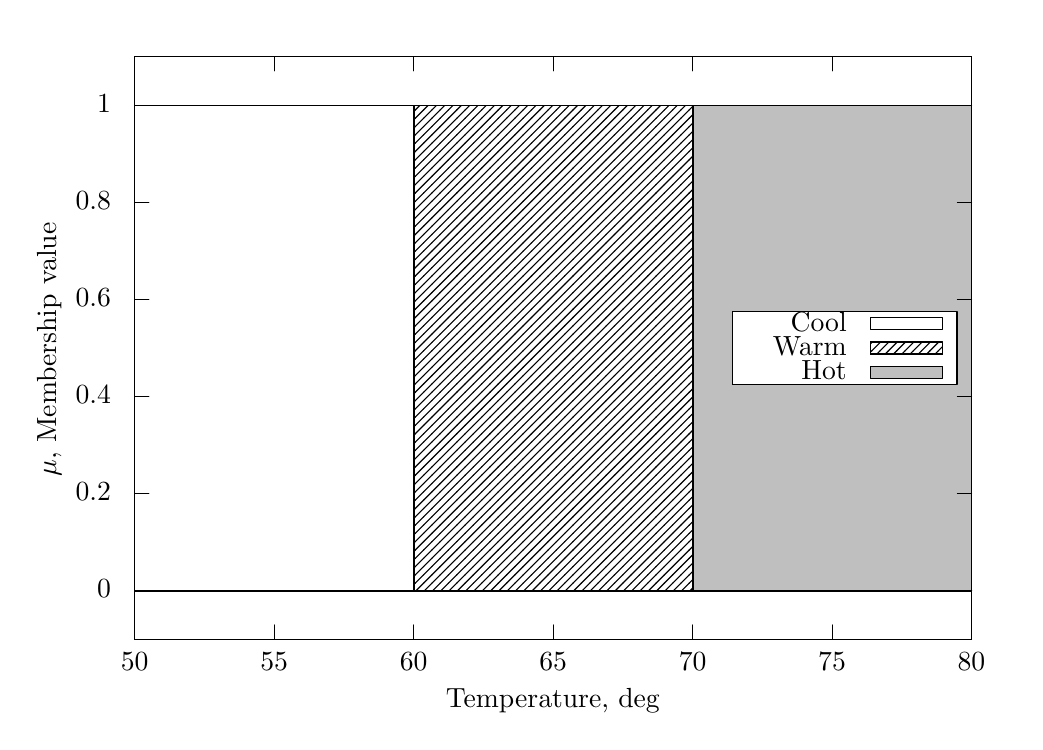
\begin{tikzpicture}[gnuplot]
%% generated with GNUPLOT 5.0p3 (Lua 5.1; terminal rev. 99, script rev. 100)
%% Thu 29 Mar 2018 12:26:43 AM EDT
\gpmonochromelines
\path (0.000,0.000) rectangle (12.500,8.750);
\gpcolor{color=gp lt color border}
\gpsetlinetype{gp lt border}
\gpsetdashtype{gp dt solid}
\gpsetlinewidth{1.00}
\draw[gp path] (1.320,1.601)--(1.500,1.601);
\draw[gp path] (11.947,1.601)--(11.767,1.601);
\node[gp node right] at (1.136,1.601) {$0$};
\draw[gp path] (1.320,2.834)--(1.500,2.834);
\draw[gp path] (11.947,2.834)--(11.767,2.834);
\node[gp node right] at (1.136,2.834) {$0.2$};
\draw[gp path] (1.320,4.067)--(1.500,4.067);
\draw[gp path] (11.947,4.067)--(11.767,4.067);
\node[gp node right] at (1.136,4.067) {$0.4$};
\draw[gp path] (1.320,5.299)--(1.500,5.299);
\draw[gp path] (11.947,5.299)--(11.767,5.299);
\node[gp node right] at (1.136,5.299) {$0.6$};
\draw[gp path] (1.320,6.532)--(1.500,6.532);
\draw[gp path] (11.947,6.532)--(11.767,6.532);
\node[gp node right] at (1.136,6.532) {$0.8$};
\draw[gp path] (1.320,7.765)--(1.500,7.765);
\draw[gp path] (11.947,7.765)--(11.767,7.765);
\node[gp node right] at (1.136,7.765) {$1$};
\draw[gp path] (1.320,0.985)--(1.320,1.165);
\draw[gp path] (1.320,8.381)--(1.320,8.201);
\node[gp node center] at (1.320,0.677) {$50$};
\draw[gp path] (3.091,0.985)--(3.091,1.165);
\draw[gp path] (3.091,8.381)--(3.091,8.201);
\node[gp node center] at (3.091,0.677) {$55$};
\draw[gp path] (4.862,0.985)--(4.862,1.165);
\draw[gp path] (4.862,8.381)--(4.862,8.201);
\node[gp node center] at (4.862,0.677) {$60$};
\draw[gp path] (6.634,0.985)--(6.634,1.165);
\draw[gp path] (6.634,8.381)--(6.634,8.201);
\node[gp node center] at (6.634,0.677) {$65$};
\draw[gp path] (8.405,0.985)--(8.405,1.165);
\draw[gp path] (8.405,8.381)--(8.405,8.201);
\node[gp node center] at (8.405,0.677) {$70$};
\draw[gp path] (10.176,0.985)--(10.176,1.165);
\draw[gp path] (10.176,8.381)--(10.176,8.201);
\node[gp node center] at (10.176,0.677) {$75$};
\draw[gp path] (11.947,0.985)--(11.947,1.165);
\draw[gp path] (11.947,8.381)--(11.947,8.201);
\node[gp node center] at (11.947,0.677) {$80$};
\draw[gp path] (1.320,8.381)--(1.320,0.985)--(11.947,0.985)--(11.947,8.381)--cycle;
\node[gp node center,rotate=-270] at (0.246,4.683) {$\mu$, Membership value};
\node[gp node center] at (6.633,0.215) {Temperature, $\deg$};
\draw[gp path] (8.915,4.221)--(8.915,5.145)--(11.763,5.145)--(11.763,4.221)--cycle;
\gpfill{color=gp lt color border,gp pattern 0,pattern color=.} (1.320,7.765)--(4.862,7.765)--(4.862,1.601)--(8.405,1.601)%
    --(8.405,1.601)--(11.947,1.601)--(11.947,1.601)--cycle;
\draw[gp path] (1.320,7.765)--(4.862,7.765)--(4.862,1.601)--(8.405,1.601)--(11.947,1.601);
\gpfill{color=gp lt color border,gp pattern 1,pattern color=.} (1.320,1.601)--(4.862,1.601)--(4.862,7.765)--(8.405,7.765)%
    --(8.405,1.601)--(11.947,1.601)--(11.947,1.601)--cycle;
\gpsetdashtype{gp dt 2}
\draw[gp path] (1.320,1.601)--(4.862,1.601)--(4.862,7.765)--(8.405,7.765)--(8.405,1.601)%
  --(11.947,1.601);
\gpfill{color=gp lt color border,opacity=0.25} (1.320,1.601)--(4.862,1.601)--(4.862,1.601)--(8.405,1.601)%
    --(8.405,7.765)--(11.947,7.765)--(11.947,1.601)--cycle;
\gpsetdashtype{gp dt 3}
\draw[gp path] (1.320,1.601)--(4.862,1.601)--(8.405,1.601)--(8.405,7.765)--(11.947,7.765)%
  --(11.947,1.601);
\gpfill{color=gpbgfillcolor} (8.915,4.221)--(11.763,4.221)--(11.763,5.145)--(8.915,5.145)--cycle;
\gpsetdashtype{gp dt solid}
\draw[gp path] (8.915,4.221)--(8.915,5.145)--(11.763,5.145)--(11.763,4.221)--cycle;
\node[gp node right] at (10.479,4.991) {Cool};
\gpfill{color=gp lt color border,gp pattern 0,pattern color=.} (10.663,4.914)--(11.579,4.914)--(11.579,5.068)--(10.663,5.068)--cycle;
\draw[gp path] (10.663,4.914)--(11.579,4.914)--(11.579,5.068)--(10.663,5.068)--cycle;
\node[gp node right] at (10.479,4.683) {Warm};
\gpfill{color=gp lt color border,gp pattern 1,pattern color=.} (10.663,4.606)--(11.579,4.606)--(11.579,4.760)--(10.663,4.760)--cycle;
\gpsetdashtype{gp dt 2}
\draw[gp path] (10.663,4.606)--(11.579,4.606)--(11.579,4.760)--(10.663,4.760)--cycle;
\node[gp node right] at (10.479,4.375) {Hot};
\gpfill{color=gp lt color border,opacity=0.25} (10.663,4.298)--(11.579,4.298)--(11.579,4.452)--(10.663,4.452)--cycle;
\gpsetdashtype{gp dt 3}
\draw[gp path] (10.663,4.298)--(11.579,4.298)--(11.579,4.452)--(10.663,4.452)--cycle;
\gpsetdashtype{gp dt solid}
\draw[gp path] (1.320,8.381)--(1.320,0.985)--(11.947,0.985)--(11.947,8.381)--cycle;
%% coordinates of the plot area
\gpdefrectangularnode{gp plot 1}{\pgfpoint{1.320cm}{0.985cm}}{\pgfpoint{11.947cm}{8.381cm}}
\end{tikzpicture}
%% gnuplot variables

    \caption{Crisp (classical) logic set transitions are discrete and abrupt}\label{f:crispsets}
\end{figure}

\begin{figure}[ht]
    \centering
    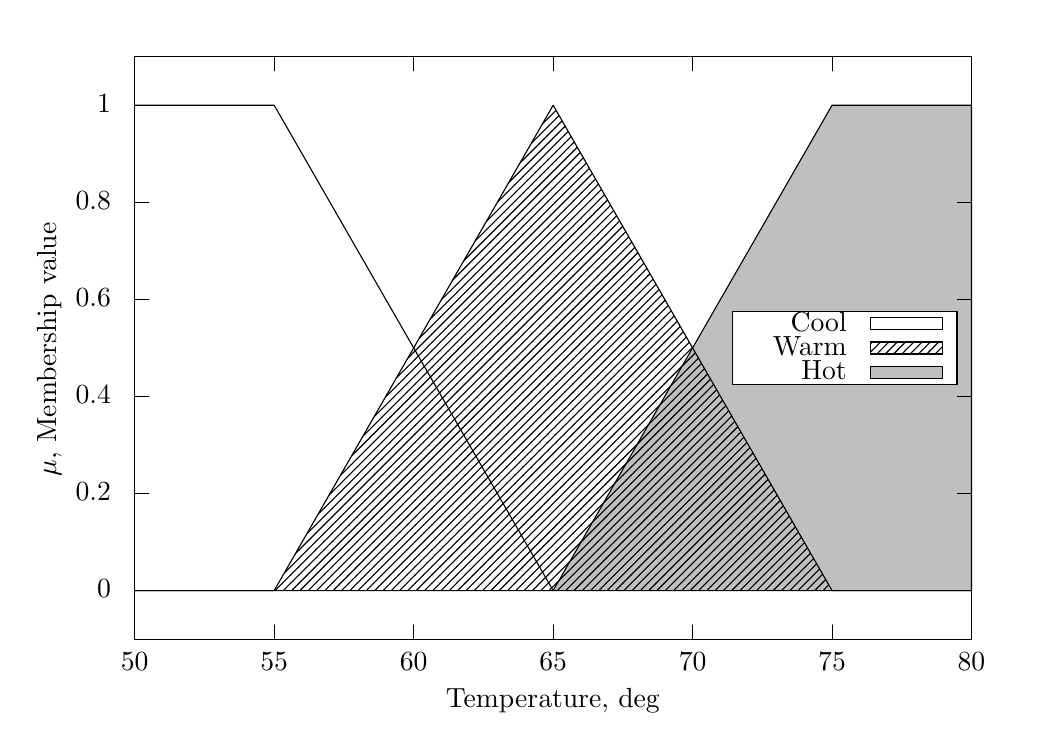
\begin{tikzpicture}[gnuplot]
%% generated with GNUPLOT 5.0p3 (Lua 5.1; terminal rev. 99, script rev. 100)
%% Thu 29 Mar 2018 12:26:43 AM EDT
\gpmonochromelines
\path (0.000,0.000) rectangle (12.500,8.750);
\gpcolor{color=gp lt color border}
\gpsetlinetype{gp lt border}
\gpsetdashtype{gp dt solid}
\gpsetlinewidth{1.00}
\draw[gp path] (1.320,1.601)--(1.500,1.601);
\draw[gp path] (11.947,1.601)--(11.767,1.601);
\node[gp node right] at (1.136,1.601) {$0$};
\draw[gp path] (1.320,2.834)--(1.500,2.834);
\draw[gp path] (11.947,2.834)--(11.767,2.834);
\node[gp node right] at (1.136,2.834) {$0.2$};
\draw[gp path] (1.320,4.067)--(1.500,4.067);
\draw[gp path] (11.947,4.067)--(11.767,4.067);
\node[gp node right] at (1.136,4.067) {$0.4$};
\draw[gp path] (1.320,5.299)--(1.500,5.299);
\draw[gp path] (11.947,5.299)--(11.767,5.299);
\node[gp node right] at (1.136,5.299) {$0.6$};
\draw[gp path] (1.320,6.532)--(1.500,6.532);
\draw[gp path] (11.947,6.532)--(11.767,6.532);
\node[gp node right] at (1.136,6.532) {$0.8$};
\draw[gp path] (1.320,7.765)--(1.500,7.765);
\draw[gp path] (11.947,7.765)--(11.767,7.765);
\node[gp node right] at (1.136,7.765) {$1$};
\draw[gp path] (1.320,0.985)--(1.320,1.165);
\draw[gp path] (1.320,8.381)--(1.320,8.201);
\node[gp node center] at (1.320,0.677) {$50$};
\draw[gp path] (3.091,0.985)--(3.091,1.165);
\draw[gp path] (3.091,8.381)--(3.091,8.201);
\node[gp node center] at (3.091,0.677) {$55$};
\draw[gp path] (4.862,0.985)--(4.862,1.165);
\draw[gp path] (4.862,8.381)--(4.862,8.201);
\node[gp node center] at (4.862,0.677) {$60$};
\draw[gp path] (6.634,0.985)--(6.634,1.165);
\draw[gp path] (6.634,8.381)--(6.634,8.201);
\node[gp node center] at (6.634,0.677) {$65$};
\draw[gp path] (8.405,0.985)--(8.405,1.165);
\draw[gp path] (8.405,8.381)--(8.405,8.201);
\node[gp node center] at (8.405,0.677) {$70$};
\draw[gp path] (10.176,0.985)--(10.176,1.165);
\draw[gp path] (10.176,8.381)--(10.176,8.201);
\node[gp node center] at (10.176,0.677) {$75$};
\draw[gp path] (11.947,0.985)--(11.947,1.165);
\draw[gp path] (11.947,8.381)--(11.947,8.201);
\node[gp node center] at (11.947,0.677) {$80$};
\draw[gp path] (1.320,8.381)--(1.320,0.985)--(11.947,0.985)--(11.947,8.381)--cycle;
\node[gp node center,rotate=-270] at (0.246,4.683) {$\mu$, Membership value};
\node[gp node center] at (6.633,0.215) {Temperature, $\deg$};
\draw[gp path] (8.915,4.221)--(8.915,5.145)--(11.763,5.145)--(11.763,4.221)--cycle;
\gpfill{color=gp lt color border,gp pattern 0,pattern color=.} (1.320,7.765)--(3.091,7.765)--(6.634,1.601)--(10.176,1.601)%
    --(11.947,1.601)--(11.947,1.601)--cycle;
\draw[gp path] (1.320,7.765)--(3.091,7.765)--(6.634,1.601)--(10.176,1.601)--(11.947,1.601);
\gpfill{color=gp lt color border,gp pattern 1,pattern color=.} (1.320,1.601)--(3.091,1.601)--(6.634,7.765)--(10.176,1.601)%
    --(11.947,1.601)--(11.947,1.601)--cycle;
\gpsetdashtype{gp dt 2}
\draw[gp path] (1.320,1.601)--(3.091,1.601)--(6.634,7.765)--(10.176,1.601)--(11.947,1.601);
\gpfill{color=gp lt color border,opacity=0.25} (1.320,1.601)--(3.091,1.601)--(6.634,1.601)--(10.176,7.765)%
    --(11.947,7.765)--(11.947,1.601)--cycle;
\gpsetdashtype{gp dt 3}
\draw[gp path] (1.320,1.601)--(3.091,1.601)--(6.634,1.601)--(10.176,7.765)--(11.947,7.765)%
  --(11.947,1.601);
\gpfill{color=gpbgfillcolor} (8.915,4.221)--(11.763,4.221)--(11.763,5.145)--(8.915,5.145)--cycle;
\gpsetdashtype{gp dt solid}
\draw[gp path] (8.915,4.221)--(8.915,5.145)--(11.763,5.145)--(11.763,4.221)--cycle;
\node[gp node right] at (10.479,4.991) {Cool};
\gpfill{color=gp lt color border,gp pattern 0,pattern color=.} (10.663,4.914)--(11.579,4.914)--(11.579,5.068)--(10.663,5.068)--cycle;
\draw[gp path] (10.663,4.914)--(11.579,4.914)--(11.579,5.068)--(10.663,5.068)--cycle;
\node[gp node right] at (10.479,4.683) {Warm};
\gpfill{color=gp lt color border,gp pattern 1,pattern color=.} (10.663,4.606)--(11.579,4.606)--(11.579,4.760)--(10.663,4.760)--cycle;
\gpsetdashtype{gp dt 2}
\draw[gp path] (10.663,4.606)--(11.579,4.606)--(11.579,4.760)--(10.663,4.760)--cycle;
\node[gp node right] at (10.479,4.375) {Hot};
\gpfill{color=gp lt color border,opacity=0.25} (10.663,4.298)--(11.579,4.298)--(11.579,4.452)--(10.663,4.452)--cycle;
\gpsetdashtype{gp dt 3}
\draw[gp path] (10.663,4.298)--(11.579,4.298)--(11.579,4.452)--(10.663,4.452)--cycle;
\gpsetdashtype{gp dt solid}
\draw[gp path] (1.320,8.381)--(1.320,0.985)--(11.947,0.985)--(11.947,8.381)--cycle;
%% coordinates of the plot area
\gpdefrectangularnode{gp plot 1}{\pgfpoint{1.320cm}{0.985cm}}{\pgfpoint{11.947cm}{8.381cm}}
\end{tikzpicture}
%% gnuplot variables

    \caption{Fuzzy sets allow for multiple membership, so a value can smoothly transition from being a member
    of one set to another.}\label{f:fuzzysets}
\end{figure}

A fuzzy inference system (FIS) is a control system built on the basic principles of fuzzy
logic\cite{kosko:91bk}\cite{kosko:93sciam}. It can take an arbitrary number of analog inputs and map them to a
set of logical variables ranging from 0 to 1. This mapping is performed by membership functions (MF), which
determine the degree of membership each input has to a function. Each input typically has multiple MFs,
allowing the input value (a so-called ``crisp value'' to be given membership in multiple sets simultaneously.
The memberships are used to make an inference about the input according to linguistic rules.  The RB is
composed of IF-THEN statements which determine the crisp output variable. For example, if the membership sets
in \cref{f:fuzzysets} were to be the input to a fan controller, and the output membership functions were as
they are in \cref{f:outputfan}, the rules could be described as:

\vspace{2em}
\begin{tabular}{cccccc}
        IF &  \emph{temperature} is & COOL, & THEN & \emph{fan speed} is & OFF\\
        IF &  \emph{temperature} is & WARM, & THEN & \emph{fan speed} is & LOW\\
        IF &  \emph{temperature} is & HOT,  & THEN & \emph{fan speed} is & HIGH
\end{tabular}
\vspace{2em}

These rules can be succinctly placed in a table as shown in \cref{t:fanspeed}. This representation becomes
more useful still as another input is added to the controller. By using the set of rules and the MFs, the FIS
is able to determine an appropriate crisp output given a set of crisp inputs. The FIS representation is in
essence a transfer function, but a transfer function which can be arbitrarily complex. The common
representation of a FIS shown in \cref{f:fis_block} shows the components of a FIS.

\begin{table}[ht]
    \centering
    \caption{Example rule base for a fictitious fan speed controller}\label{t:fanspeed}
    \begin{tabular}{c|c|c|c}
        Temperature & Cool & Warm & Hot\\\hline
        Fan Speed & Off & Low & High
    \end{tabular}
\end{table}

\begin{figure}[ht]
    \centering
    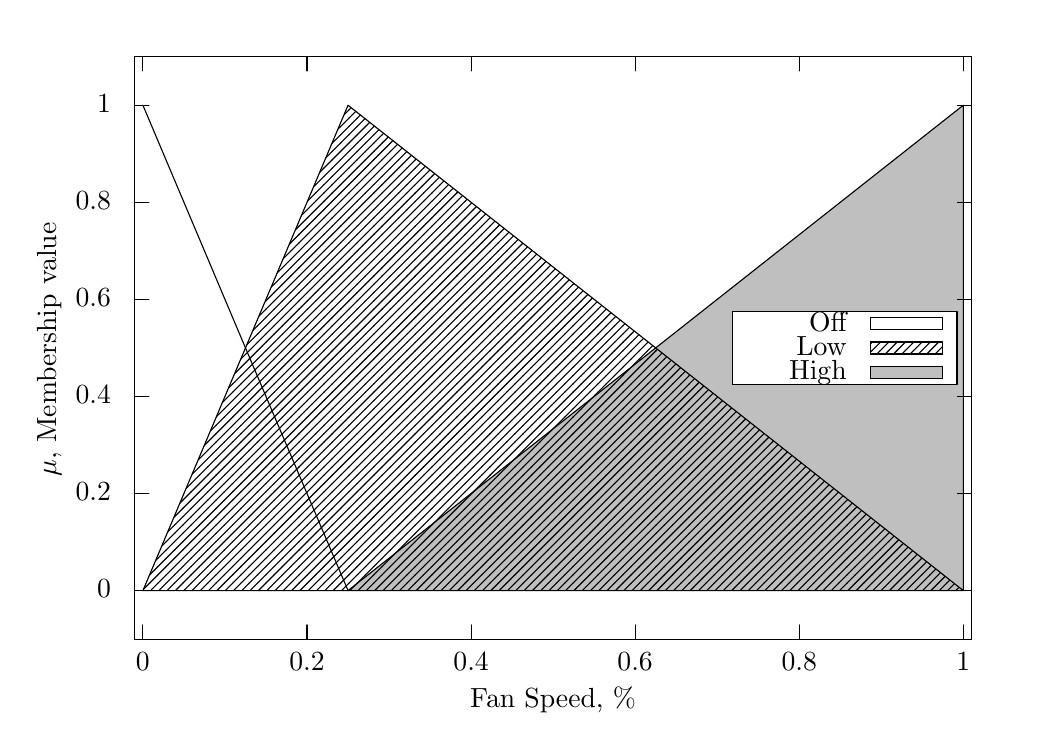
\begin{tikzpicture}[gnuplot]
%% generated with GNUPLOT 5.0p3 (Lua 5.1; terminal rev. 99, script rev. 100)
%% Thu 29 Mar 2018 12:26:43 AM EDT
\gpmonochromelines
\path (0.000,0.000) rectangle (12.500,8.750);
\gpcolor{color=gp lt color border}
\gpsetlinetype{gp lt border}
\gpsetdashtype{gp dt solid}
\gpsetlinewidth{1.00}
\draw[gp path] (1.320,1.601)--(1.500,1.601);
\draw[gp path] (11.947,1.601)--(11.767,1.601);
\node[gp node right] at (1.136,1.601) {$0$};
\draw[gp path] (1.320,2.834)--(1.500,2.834);
\draw[gp path] (11.947,2.834)--(11.767,2.834);
\node[gp node right] at (1.136,2.834) {$0.2$};
\draw[gp path] (1.320,4.067)--(1.500,4.067);
\draw[gp path] (11.947,4.067)--(11.767,4.067);
\node[gp node right] at (1.136,4.067) {$0.4$};
\draw[gp path] (1.320,5.299)--(1.500,5.299);
\draw[gp path] (11.947,5.299)--(11.767,5.299);
\node[gp node right] at (1.136,5.299) {$0.6$};
\draw[gp path] (1.320,6.532)--(1.500,6.532);
\draw[gp path] (11.947,6.532)--(11.767,6.532);
\node[gp node right] at (1.136,6.532) {$0.8$};
\draw[gp path] (1.320,7.765)--(1.500,7.765);
\draw[gp path] (11.947,7.765)--(11.767,7.765);
\node[gp node right] at (1.136,7.765) {$1$};
\draw[gp path] (1.424,0.985)--(1.424,1.165);
\draw[gp path] (1.424,8.381)--(1.424,8.201);
\node[gp node center] at (1.424,0.677) {$0$};
\draw[gp path] (3.508,0.985)--(3.508,1.165);
\draw[gp path] (3.508,8.381)--(3.508,8.201);
\node[gp node center] at (3.508,0.677) {$0.2$};
\draw[gp path] (5.592,0.985)--(5.592,1.165);
\draw[gp path] (5.592,8.381)--(5.592,8.201);
\node[gp node center] at (5.592,0.677) {$0.4$};
\draw[gp path] (7.675,0.985)--(7.675,1.165);
\draw[gp path] (7.675,8.381)--(7.675,8.201);
\node[gp node center] at (7.675,0.677) {$0.6$};
\draw[gp path] (9.759,0.985)--(9.759,1.165);
\draw[gp path] (9.759,8.381)--(9.759,8.201);
\node[gp node center] at (9.759,0.677) {$0.8$};
\draw[gp path] (11.843,0.985)--(11.843,1.165);
\draw[gp path] (11.843,8.381)--(11.843,8.201);
\node[gp node center] at (11.843,0.677) {$1$};
\draw[gp path] (1.320,8.381)--(1.320,0.985)--(11.947,0.985)--(11.947,8.381)--cycle;
\node[gp node center,rotate=-270] at (0.246,4.683) {$\mu$, Membership value};
\node[gp node center] at (6.633,0.215) {Fan Speed, $\%$};
\draw[gp path] (8.915,4.221)--(8.915,5.145)--(11.763,5.145)--(11.763,4.221)--cycle;
\gpfill{color=gp lt color border,gp pattern 0,pattern color=.} (1.424,7.765)--(4.029,1.601)--(11.843,1.601)--(11.843,1.601)--cycle;
\draw[gp path] (1.424,7.765)--(4.029,1.601)--(11.843,1.601);
\gpfill{color=gp lt color border,gp pattern 1,pattern color=.} (1.424,1.601)--(4.029,7.765)--(11.843,1.601)--(11.843,1.601)--cycle;
\gpsetdashtype{gp dt 2}
\draw[gp path] (1.424,1.601)--(4.029,7.765)--(11.843,1.601);
\gpfill{color=gp lt color border,opacity=0.25} (1.424,1.601)--(4.029,1.601)--(11.843,7.765)--(11.843,1.601)--cycle;
\gpsetdashtype{gp dt 3}
\draw[gp path] (1.424,1.601)--(4.029,1.601)--(11.843,7.765)--(11.843,1.601);
\gpfill{color=gpbgfillcolor} (8.915,4.221)--(11.763,4.221)--(11.763,5.145)--(8.915,5.145)--cycle;
\gpsetdashtype{gp dt solid}
\draw[gp path] (8.915,4.221)--(8.915,5.145)--(11.763,5.145)--(11.763,4.221)--cycle;
\node[gp node right] at (10.479,4.991) {Off};
\gpfill{color=gp lt color border,gp pattern 0,pattern color=.} (10.663,4.914)--(11.579,4.914)--(11.579,5.068)--(10.663,5.068)--cycle;
\draw[gp path] (10.663,4.914)--(11.579,4.914)--(11.579,5.068)--(10.663,5.068)--cycle;
\node[gp node right] at (10.479,4.683) {Low};
\gpfill{color=gp lt color border,gp pattern 1,pattern color=.} (10.663,4.606)--(11.579,4.606)--(11.579,4.760)--(10.663,4.760)--cycle;
\gpsetdashtype{gp dt 2}
\draw[gp path] (10.663,4.606)--(11.579,4.606)--(11.579,4.760)--(10.663,4.760)--cycle;
\node[gp node right] at (10.479,4.375) {High};
\gpfill{color=gp lt color border,opacity=0.25} (10.663,4.298)--(11.579,4.298)--(11.579,4.452)--(10.663,4.452)--cycle;
\gpsetdashtype{gp dt 3}
\draw[gp path] (10.663,4.298)--(11.579,4.298)--(11.579,4.452)--(10.663,4.452)--cycle;
\gpsetdashtype{gp dt solid}
\draw[gp path] (1.320,8.381)--(1.320,0.985)--(11.947,0.985)--(11.947,8.381)--cycle;
%% coordinates of the plot area
\gpdefrectangularnode{gp plot 1}{\pgfpoint{1.320cm}{0.985cm}}{\pgfpoint{11.947cm}{8.381cm}}
\end{tikzpicture}
%% gnuplot variables

    \caption{Possible output membership functions for a fan controller with \cref{f:fuzzysets} as the
    input.}\label{f:outputfan}
\end{figure}

\begin{figure}[ht]
    \centering
    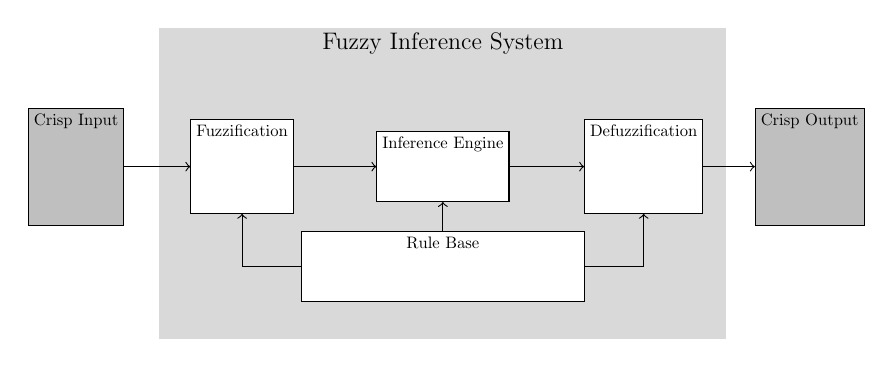
\begin{tikzpicture}[scale=0.6, transform shape]
    \node[fill=gray!30,text depth = 6cm,minimum width=12cm,font=\Large] (main){Fuzzy Inference System};
    \node[draw,fill=white!30, text depth=1cm] at ([yshift=1em]main.center)(infer){Inference Engine};
    \node[draw,fill=white!30, text depth=1cm, minimum width=6cm] at ([yshift=-5em]main.center)(rb){Rule Base};
    \node[draw,fill=white!30, text depth=1.5cm] at ([xshift=5em, yshift=1em]main.west)(fuzz){Fuzzification};
    \node[draw,fill=white!30, text depth=1.5cm] at ([xshift=-5em, yshift=1em]main.east)(defuzz){Defuzzification};
    \node[draw,fill=gray!50, text depth=2cm] at ([xshift=-5em, yshift=1em]main.west)(inp){Crisp Input};
    \node[draw,fill=gray!50, text depth=2cm] at ([xshift=5em, yshift=1em]main.east)(outp){Crisp Output};

    \node at ([xshift=5em, yshift=-5em]main.west)(ghostleft){};
    \node at ([xshift=-5em, yshift=-5em]main.east)(ghostright){};

    \draw[->](inp.east) -- (fuzz.west);
    \draw[->](fuzz.east) -- (infer.west);
    \draw[->](infer.east) -- (defuzz.west);
    \draw[->](defuzz.east) -- (outp.west);
    \draw[->](rb.north) -- (infer.south);
    \draw[->](rb.west) -- (ghostleft.center) -- (fuzz.south);
    \draw[->](rb.east) -- (ghostright.center) -- (defuzz.south);
\end{tikzpicture}

    \caption{Visual representation of a fuzzy inference system}\label{f:fis_block}
\end{figure}

One limiting constraint of FL systems is manifested in a type of state explosion. As the number of inputs,
specifically the number of input MFs, increases, the number of rules needed to cover every case increases as
the product of the number of MFs across all inputs. There have been numerous approaches to overcome this
problem such as cascading small FISs together\cite{ernest2015genetic}, developing more robust methods to guide
convergence\cite{hansen1997convergence} or using approximate fuzzy rule bases\cite{cordon:01bk}. The approach
taken in this work, however, has been to employ GA techniques to tune the MFs or even learn the entire
knowledge base. The dynamic systems being controlled in this research are adequately small such that no
special state reduction was deemed necessary in most cases.

\section{Genetic Algorithms}
Genetic algorithms are an evolutionary computing strategy commonly used in optimization and search problems
\cite{bodenhofer1997ten}. Their effectiveness comes from the combined ability to explore and exploit. The
exploration of even large search spaces is made possible with large populations of candidate solutions which
are stochastically sampled across the whole space. Candidates are ranked according to a fitness function and
recombined together to create the next generation. The algorithm exploits learning in the selection process,
favoring recombination of candidates which ranked well according to the fitness function. In order to maintain
gene pool diversity, random mutation is introduced into each generation as it is created. This process is
illustrated in \cref{f:ga_block}. Due to the stochastic nature of the algorithm, it is not guaranteed to
provide an optimal solution and may converge on a local optimum, but careful selection of hyper parameters
such as population size, mutation rates, recombination methods, and random candidate injection can  somewhat
circumvent these deficiencies. As the goal of a GA is to maximize some definition of a reward, they are
commonly employed in reinforcement learning applications\cite{salimans2017evolution}.

\begin{figure}[ht]
    \centering
    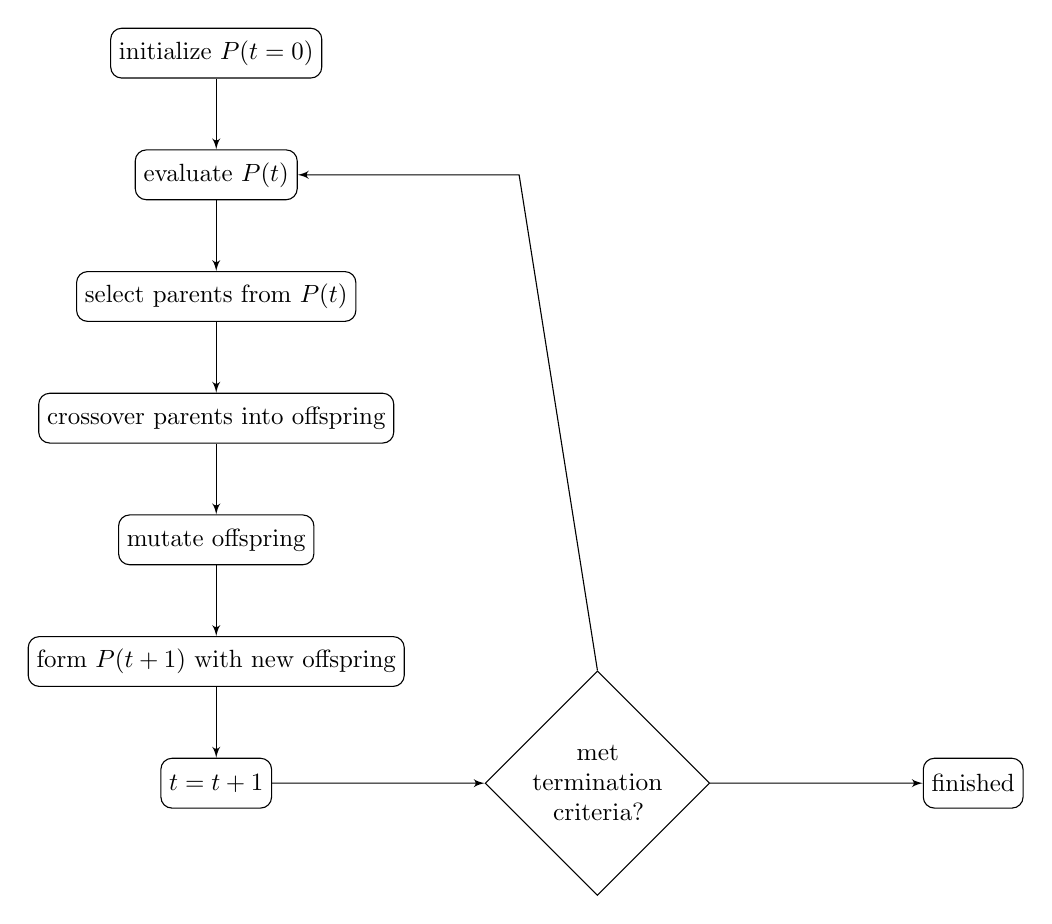
\begin{tikzpicture}[node distance=1cm and 3cm, auto, scale = 0.9, transform shape]
\node[draw, block] (init){initialize $P(t=0)$};
\node[draw, block, below= of init](eval){evaluate $P(t)$};
\node[draw, block, below= of eval](select){select parents from $P(t)$};
\node[draw, block, below= of select](cross){crossover parents into offspring};
\node[draw, block, below= of cross](mut){mutate offspring};
\node[draw, block, below= of mut](ass){form $P(t+1)$ with new offspring};
\node[draw, block, below= of ass](iter){$t=t+1$};
\node[draw, decision, right= of iter](term){met\\termination criteria?};
\node[draw, block, right= of term](fin){finished};

\node [right= of eval](dummy1){};

\draw[line](init) -- (eval);
\draw[line](eval) -- (select);
\draw[line](select) -- (cross);
\draw[line](cross) -- (mut);
\draw[line](mut) -- (ass);
\draw[line](ass) -- (iter);
\draw[line](iter) -- (term);
\draw[line](term) -- (fin);
\draw[line](term.north) -- (dummy1.center) -- (eval);
\end{tikzpicture}

    \caption{Block diagram describing genetic algorithm}\label{f:ga_block}
\end{figure}

Since the fitness function is the sole driver of the algorithm and the solution it provides, great care must
be taken in formulating a fitness function. In robotics applications in particular, formulating a fitness
which adequately encapsulates complex outcomes can be a difficult task\cite{divband2015effect}. This issue
will be revisited a number of times throughout the course of this work.

Another major consideration when utilizing a GA is how to represent or encode a candidate solution for
optimization. A particularly simple method is to use a binary encoded format\cite{cordon:01bk}, but this
increases the distance between the candidate in its useful form (phenotype) and its encoded form (genotype)
for many real-values problems\cite{chakraborty1991chromosomal}. A genetic encoding of a FIS is an inherently
heterogeneous structure with real values describing the MFs and discrete classes describing the RB. The
genetic operator chosen for a specific genotype will depend on its representation; ideally, the mapping
between genotype and phenotype will be one-to-one such that the combination of two genes will produce a
candidate which performs similarly to its parents. This allows the GA to properly exploit its inherent
learning and converge on a solution.

\subsection{Genetic Operators}
The GA advances by applying operations to the chromosome candidates in its population. The genetic operations
employed in this work are crossover,  mutation, and randomization. Crossover is the operation which allows the
genes from two chromosomes to mix and create new children. If the chromosomes are binary encoded or discrete
valued, the crossover method is generally single-, double-, or n-point crossover. This involves randomly
selecting a point in the encoding string to ``cut'' the chromosomes and swap the tails for single-point, or
sections for n-point.  \Cref{f:dp_cx} demonstrates this process. 



\begin{figure}[ht]
    \centering
    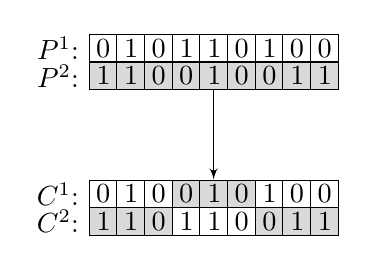
\begin{tikzpicture}[node distance = 0pt]
    \node[dad](d0){0};
    \node[dad, right of=d0](d1){1};
    \node[dad, right of=d1](d2){0};
    \node[dad, right of=d2](d3){1};
    \node[dad, right of=d3](d4){1};
    \node[dad, right of=d4](d5){0};
    \node[dad, right of=d5](d6){1};
    \node[dad, right of=d6](d7){0};
    \node[dad, right of=d7](d8){0};
    \node[mom, below of = d0](m0){1};
    \node[mom, right of=m0](m1){1};
    \node[mom, right of=m1](m2){0};
    \node[mom, right of=m2](m3){0};
    \node[mom, right of=m3](m4){1};
    \node[mom, right of=m4](m5){0};
    \node[mom, right of=m5](m6){0};
    \node[mom, right of=m6](m7){1};
    \node[mom, right of=m7](m8){1};
    \node[left =of d0] {$P^1$:};
    \node[left =of m0] {$P^2$:};

    \node[dad, below of=d0, yshift=-1.5cm](c0){0};
    \node[dad, right of=c0](c1){1};
    \node[dad, right of=c1](c2){0};
    \node[mom, right of=c2](c3){0};
    \node[mom, right of=c3](c4){1};
    \node[mom, right of=c4](c5){0};
    \node[dad, right of=c5](c6){1};
    \node[dad, right of=c6](c7){0};
    \node[dad, right of=c7](c8){0};
    \node[mom, below of = c0](b0){1};
    \node[mom, right of=b0](b1){1};
    \node[mom, right of=b1](b2){0};
    \node[dad, right of=b2](b3){1};
    \node[dad, right of=b3](b4){1};
    \node[dad, right of=b4](b5){0};
    \node[mom, right of=b5](b6){0};
    \node[mom, right of=b6](b7){1};
    \node[mom, right of=b7](b8){1};
    \node[left =of c0] {$C^1$:};
    \node[left =of b0] {$C^2$:};

    \draw[line](m4) -- (c4);
\end{tikzpicture}

    \caption{Double point crossover for binary or discrete valued chromosome.}\label{f:dp_cx}
\end{figure}

For real-valued chromosome strings, the crossover methods can be much more complex and more closely related to
solution space. Throughout this work, variations on flat crossover will be employed as the main crossover
operation for real-valued portions of the chromosomes\cite{cordon:01bk}. Using this method, a new gene is
created from its parents by drawing a real value from the interval between the parent genes using a uniform
distribution. In many situations, it becomes simpler to write code which always produces two children from a
pair of parents; in these cases, the other gene from a parent interval is selected to be the complement of the
first. Given parents, $P^1 = \left\{p_1^1, p_2^1, \dots, p_n^1\right\},\,P^2=\left\{p_1^2,p_2^2, \dots,
p_n^2\right\}$, children
$C^1=\left\{c_1^1, c_2^1, \dots, c_n^1\right\},\,C^2=\left\{c_1^2,c_2^2,\dots,c_n^2\right\}$ are
created such that:

\begin{align}
    c_i^1 &= \lambda p_i^{min} + (1 - \lambda)p_i^{max}\label{e:flat_cx_c1}\\
    c_i^2 &= (1-\lambda)p_i^{min} + \lambda p_i^{max}\label{e:flat_cx_c2}
\end{align}
where $p_i^{max}=\max(p_i^1,p_i^2)$ and $p_i^{min}=\min(p_i^1,p_i^2)$. An extension, \emph{BLX-$\alpha$}
crossover, is used to expand the selection region beyond the interval between the parents to allow the
crossover function to be more exploratory\cite{cordon:01bk}. This method is described in more detail in
\cref{c:acc}.

Mutation for discrete-valued chromosomes consists of randomly choosing a value from the set of possible values
for a number of genes in a chromosome. For this work, mutation is applied to the chromosomes after crossover is
applied. The number of genes in each chromosome to mutate is defined as a hyperparameter. Mutation for
real-valued chromosomes is done with a non-uniform mutation rate which decreases as the generations progress.
This process is detailed in \cref{c:acc}.

For each new generation of chromosomes, a small number of the best performers are preserved untouched from the
previous generation to allow the best genetic material to survive. These chromosomes are called elite. All
chromosomes are ranked according to their fitness to the task and used in crossover proportional to their
fitness. In other words, parents are selected for mutation by drawing chromosomes from the ranked list of
chromosomes using a triangular distribution. \Cref{f:sort-select} shows a distribution laid on top of a sorted
population from which parents would be selected for  recombination. Parents are replaced after selection so
that they may reproduce many times in one generation.

\begin{figure}
    \centering
    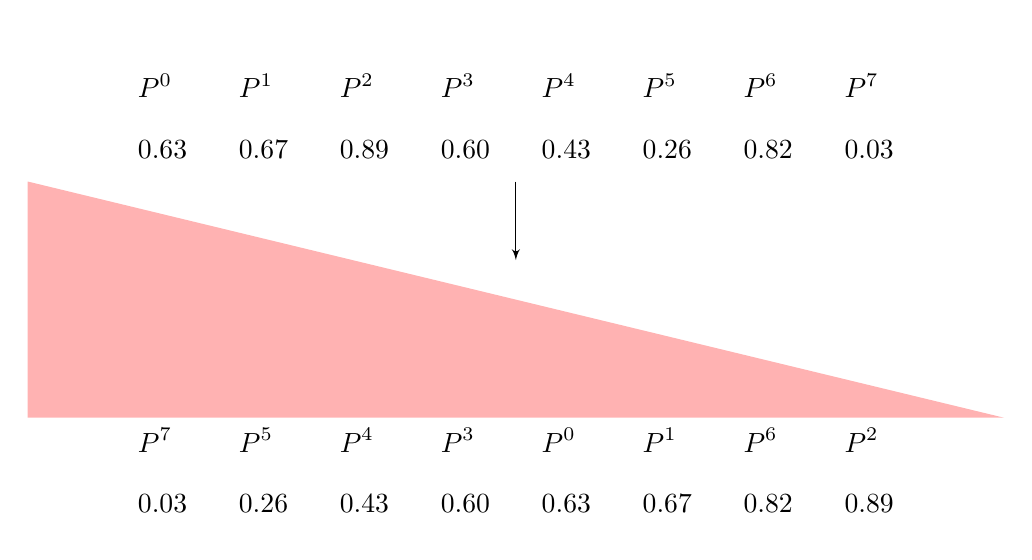
\begin{tikzpicture}
    \draw[fill=red!30, draw=none](-6.2,-1) -- (6.2,-4) -- (-6.2,-4) -- cycle;
    \node(presort){
            \begin{minipage}{0.9\textwidth}
                \begin{align*}
                    &P^{0}&&P^{1}&&P^{2}&&P^{3}&&P^{4}&&P^{5}&&P^{6}&&P^{7}\\
                    &0.63&&0.67&&0.89&&0.60&&0.43&&0.26&&0.82&&0.03
                \end{align*}
            \end{minipage}
        };
    \node[below of= presort, yshift=-3.5cm] (sorted){
            \begin{minipage}{0.9\textwidth}
                \begin{align*}
                    &P^{7}&&P^{5}&&P^{4}&&P^{3}&&P^{0}&&P^{1}&&P^{6}&&P^{2}\\
                    &0.03&&0.26&&0.43&&0.60&&0.63&&0.67&&0.82&&0.89
                \end{align*}
            \end{minipage}
        };
    \draw[line](0,-1) -- (0,-2);

\end{tikzpicture}




    \caption{Population sorting and selection distribution overlay}\label{f:sort-select}
\end{figure}
    
\section{Genetic Fuzzy Systems}
Genetic Fuzzy Systems (GFS) here describe FL systems which have been tuned or learned using GA strategies.
Tuning a GFS implies that the rule base is static, while the GA is allowed to operate on only the MF values or
input/output scaling. Learning, on the other hand, implies that the RB itself is allowed to vary. For this
research, except where otherwise stated, GFSs are allowed to learn the RB from scratch. In order to
effectively use GAs to interact with FISs, some simplifying constraints are commonly imposed on the GFS to
ease the use of genetic operators. One such constraint that is frequently used in this research is to mandate
strict triangular or trapezoidal MFs. This allows the entire collection of MFs across all of the inputs to be
described by either 3- or 4-tuples of sorted real values. As the GA is allowed to operate on the MFs, checks
are placed to make sure that like MFs are recombined and that the children contain valid MFs.  All of this is
eased by constraining a GFS to only contain triangular or trapezoidal MFs. Additionally, it is assumed that
the RB completely covers the input combination possibilities. This is similar to a fully connected layer of
neurons in a NN. This forces the number of rules to be equal to the product of the number of MFs across all
inputs; as a result of this constraint, the number of rules can quickly explode as inputs are added to the
system or inputs are granularized with additional MFs. To prevent RB explosion, FISs in this work are kept
minimal. Knowing the number of MFs, the RB can be reduced to a single string of integers, where each integer
is equal to the index of one of the output MFs. Thus in this way, we can fully describe a FIS with one
heterogeneous string of values. For instance, the FIS illustrated in \crefrange{f:fuzzysets}{f:outputfan} with
the RB in \cref{t:fanspeed} would be described completely by the list:

\begin{equation*}
    \left(0, 0, 55, 65\right) \left(55, 65, 75\right) \left(65, 75, 100, 100\right)
    |\left(0, 0, 0.25\right) \left(0, 0.25, 1\right) \left(0.25, 1, 1\right)
    \left[0, 1, 2\right]
\end{equation*}
where each MF tuple is grouped in $\left(\right)$, input is separated from output with $|$, and the RB is in
$\left[\,\right]$. The genetic operations on MF parameters are any operations which can work with real values,
and the RB is constrained to n-point crossover.

\section{Motivation and Problem Statement}
This work explores the utility of using the GFS approach to exert control on dynamic systems. Because of the
ability of a GFS to deal with imprecision and uncertainty, it can be an adaptive controller which can respond
to changes in plant dynamics. Also, if the GFS is kept small, the trained system can be interpreted by a human
operator with linguistic rules. With the rise in popularity of black box decision-making frameworks in recent
years, interpretability has become a topic of fervent
research\cite{ribeiro2016should,lipton2016mythos,zeiler2014visualizing,dong2017improving}. Learning provides
the benefit of exhibiting emergent behavior, but usually at the cost of interpretability. Genetic fuzzy
systems may provide a middle ground; starting with a hand-crafted template, and then allowing a GA to learn
behavior, the final model can still be assigned linguistic variables and given meaning. 

This thesis is composed of a handful of problems which were approached using a GFS.
\begin{enumerate}
    \item {\bf Two-cart flexible system}. First, the problem of controlling a two-cart system is addressed.
        The system is allowed to move freely along a track with the objective of meeting, but not exceeding, a
        goal. This system exhibits two modes of behavior: over large distances, it behaves similar to a rigid
        structure; when finer control is needed in the terminal phase, the flexible body vibrations dominate
        the behavior. A controller is tuned to handle this system in \cref{c:acc}.

    \item {\bf F-4 Phantom Pitch Controller}. Secondly, a pitch attitude controller for the F-4 fighter jet is
        designed. This system is allowed to train on only a nominal flight condition, but then subjected to
        large degradations in plant dynamics and evaluated. The performance is shown to exceed that of a PID
        controller in \cref{c:f4}.

    \item {\bf sUAS Precision Landing} Finally, a controller for a small quadrotor is designed to guide the
        vehicle to a moving target using only visual feedback from an on-board camera. This problem is
        constrained by physical systems, so simulation environments, controllers, computations, and sensors
        are chosen such that the system will be more readily physically realized. The use of the Robot Operating
        System with the Gazebo simulation environment are also discussed at length. This discussion comprises
        \cref{c:landing}.
\end{enumerate}



\chapter{Two-cart Flexible System}\label{c:acc}
\section{Introduction}
The 1992 American Control Conference published a set of benchmark problems to explore the capabilities of
modern control techniques\cite{wie1992benchmark}. The second stated problem solicited solutions to the
stabilization of a two-body spring mass system which was robust to uncertain masses and spring constants. This
benchmark problem focuses on disturbance rejection in minimum time. Stengel\cite{stengel1992robustness}
surveyed the best performing control strategies and quantified their stability and performance robustness
using stochastic robustness analysis. Cohen et. al \cite{cohen:01jgcd} independently proposed a solution using
fuzzy logic which has more robust stability, performance and uses less control effort.

This problem extends the benchmark problem with the addition of automatically tuned fuzzy controllers for
various plant models via a GA. The goal of the controller is to move the dual-mass system from a stationary
initial condition to a stationary end goal in minimum time. Simplifications to the problem include a
collocated sensor and actuator, removed plant disturbance, and removed sensor noise. The model dynamics are
similar to those experienced by a robotic arm moving from one control point to another. The system exhibits
both rigid and flexible body modes and thus provides a good test case for a nonlinear fuzzy controller. The
controller is first developed by hand and then automatic tuning strategies are employed using a GA. The plant
model masses are then changed significantly and the controller is retrained to test the efficacy of the GA
tuning process and to demonstrate the utility of having an automated tuning method. The result is a system
which can be quickly trained to accommodate new plant dynamics within this class of models. The performance of
the hand- and GA-tuned controllers are compared. 

\section{Coupled Spring-Mass Simulation Model}\label{s:model}
A simulated environment is necessary to test the efficacy of the proposed FIS. The simulation consists of two
cars connected by a spring; this system is expected to traverse a given distance as quickly as possible
without exceeding a certain boundary represented by a wall. The system is propelled by a force on the leading car
which represents the actuating output of the controller. At each time instant, the controller must determine
how much force to exert on the carts, and in which direction, to get as close as possible to the wall in
minimum time. The carts are represented by point masses which
may occupy the same position in space. The constants for the model are the weight of each car, the spring constant, and the distance
which must be traversed to the wall. A diagram of the simulation is shown in \cref{f:model}.

\begin{displaymath}
    m_{1}=\SI{1}{\kilogram}, \quad m_{2}=\SI{2}{\kilogram}, \quad K =
    \SI{250}{\newton\per\metre}, \quad L = \SI{100}{\metre}
\end{displaymath}
\nomenclature{$m$}{Cart mass,\si{\kilogram}}
\nomenclature{$K$}{Spring Constant, \si{\newton\per\metre}}
\nomenclature{$L$}{Simulation length, \si{\metre}}
\nomenclature[b$1$]{$1$}{Denotes property of trailing cart}
\nomenclature[b$2$]{$2$}{Denotes property of leading cart}
\nomenclature{$F$}{Control force, \si{\newton}}
\nomenclature{$t$}{Time, \si{\second}}

\begin{figure}
    \centering
    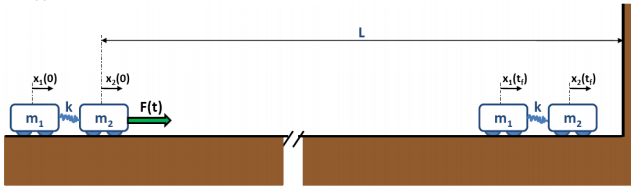
\includegraphics[width=0.9\textwidth]{images/model.png}
    \caption{Diagram of two rigid bodies connected by a spring traversing distance \textrm{L} in minimum
    time.} \label{f:model}
\end{figure}

The modeled system contains displacement and velocity sensors on each cart; therefore, the four inputs to the
FIS are the distances traveled and the velocities of both carts. These inputs represent the state vector of
the system. The output of the controller is the force, $F(t)$, applied to cart 2, limited to $\pm
\SI{1}{\newton}$. At each time step of the simulation, the FIS uses the state of cart 2 to determine the force
which must be exerted according to a fuzzy rule base. 

\begin{displaymath}
    \mathrm{Input:}\quad \vec{y}(t)= \begin{bmatrix} x_{1}(t)\\ x_{2}(t)\\ \dot{x}_{1}(t)\\
\dot{x}_{2}(t) \end{bmatrix}
\end{displaymath}
\begin{displaymath} \mathrm{Output:}\quad |F(t)|\le
\SI{1}{\newton}
\end{displaymath}
\nomenclature[1\(y\)]{$y$}{System state vector}
\nomenclature[1\(xx\)]{$\dot{x}(t)$}{Cart velocity, \si{\metre\per\second}}
\nomenclature[1\(xb\)]{$x(t)$}{Cart position, \si{\meter}}
At time $t=0$, both carts are at rest at position
$x=0$. The maximum allowed run time of the simulation is \SI{500}{\second}. The system requirement for the
final condition is that both carts come to rest between \SIrange{99}{100}{\metre} with minimal oscillation.
Neither cart is allowed at any point in the simulation to exceed \SI{100}{\metre}.
\begin{displaymath}
    \vec{y}_0=\begin{bmatrix}
\SI{0}{\metre}\\\SI{0}{\metre}\\\SI{0}{\metre\per\second}\\\SI{0}{\metre\per\second} \end{bmatrix},\quad
\vec{y}(500)=\begin{bmatrix} \SI{99}{\metre}<x_1<\SI{100}{\metre}\\ \SI{99}{\metre}<x_2<\SI{100}{\metre}\\ \SI{0}{\metre\per\second}\\
\SI{0}{\metre\per\second} \end{bmatrix}
\end{displaymath}
\nomenclature[b$0$]{$0$}{Denotes initial condition}

The acceleration of cart 1 is determined by the displacement between the two carts, the spring constant, and
the mass of the cart. The acceleration of cart 2 is also a function of these parameters as well as the control
force. The equations of motion for the system are represented by simple second-order differential equations.
\begin{equation}
\label{e:cart1} \mathrm{Cart 1:}\quad \ddot{x}_1=\frac{K}{m_1}(x_2-x_1) 
\end{equation}
\begin{equation}
    \label{e:cart2} \mathrm{Cart 2:}\quad \ddot{x}_2=\frac{K}{m_2}(x_1-x_2)+\frac{F}{m_2}
\end{equation} \nomenclature[1\(xxx\)]{$\ddot{x}(t)$}{Cart acceleration, \si{\metre\per\second\squared}}

\subsection{System Performance Cost}
The efficiency of a FIS's control of the system is based upon the amount of time
it expends traversing the distance to the wall and how close the carts are to the wall when they settle. Any
breach of the wall results in immediate system failure. A cost function, $J$, is defined by the settling time
$t_f$, the time taken to settle within \SI{1}{\metre} of the wall and the steady state error, the distance
between the leading cart and the wall. The control system that produces the lowest $J$ value will be proven
to be the most fit solution for the simulation. This cost function in particular was provided in order to
compare to results previously obtained\cite{walker:13p,vick:13p,mitchell:13p,stimetz:13p}.
\begin{equation}\label{e:timesettle}
t_f=|L-\bar{x}(t_f)|\le\SI{1}{\metre}
\end{equation} \nomenclature[b$f$]{$f$}{Denotes condition at settling time}
\begin{equation}\label{e:cost}
J=\frac{t_f}{100}+2[L-x_2(500)]
\end{equation}
where the constants 100 and 2 are scaling factors. In order to provide a frame of reference for the
performance of any control system, the theoretical limits of the simulation were calculated to provide a lower
bound for the value of \cref{e:cost}. Assuming a single rigid body assembly with no dynamic coupling, the
model is greatly simplified to a single equation where the acceleration of the body is a function of only the
control force. Since no energy is lost to a spring, the optimal solution to this system is assumed to be a
lower bound on the flexible system with losses.
\begin{equation}
    \label{e:simplemodel} \ddot{x}=\frac{F}{M}
\end{equation}
\nomenclature{$M$}{Total system mass, \si{\kilogram}}
where $M$ is the total mass of the system. The total mass of the system is \SI{3}{\kilogram}, whereas the
maximum input force is limited to \SI{1}{\newton}, rendering \cref{e:simplemodel}
\begin{displaymath}
        \ddot{x}=\frac{\SI{1}{\newton}}{\SI{3}{\metre}}=\SI[quotient-mode=fraction]{1/3}{\metre\per\second\squared}
\end{displaymath}
as the maximum acceleration. Given this acceleration and the distance to be traversed to the wall, the minimum
time to complete the trip can be calculated. There are, however, two scenarios to consider. 
\begin{enumerate} 
    \item Applying maximum force over the entire distance and instantaneously
        stopping the carts at (but not touching) the wall provides an absolute, if unfeasible, optimum
        simulation completed in minimum time. Given an initial velocity of zero and a constant accelerating
        force of \SI{1}{\newton}, the traversal time is calculated. Note that once the carts have breached
        \SI{99}{\metre}, the system may come to rest and be considered settled. 
        \begin{displaymath}
        x(t)=\dot{x}_0t+\frac{1}{2}\ddot{x}t^2,\quad \dot{x}_0=0
        \end{displaymath}
        \begin{displaymath}
        x(t)=\frac{1}{2}\ddot{x}t^2
        \end{displaymath}
        Letting $x(t) = \SI{99}{\metre}$
        \begin{displaymath}
            t=\sqrt{\frac{2x(t)}{\ddot{x}}}=\sqrt{\frac{2\cdot
            \SI{99}{\metre}}{\SI[quotient-mode=fraction]{1/3}{\metre\per\second\squared}}}=\SI{24.37}{\second}
        \end{displaymath}
    \item Applying maximum force over half of the distance and then applying maximum
        negative force in the second half to slow the velocities of the carts to zero at the wall position.

First half: \begin{displaymath}
t=\sqrt{\frac{2x(t)}{\ddot{x}}}=\sqrt{\frac{2\cdot\SI{50}{\metre}}{\SI[quotient-mode=fraction]{1/3}{\meter\per\second\squared}}}=\SI{17.23}{\second}
\end{displaymath} Traversing the second half and stopping at the wall takes the same amount of time, therefore
the total time expended in reaching \SI{100}{\metre} is \SI{34.46}{\second}; however, the interest lies in the
time taken to breach the \SI{99}{\metre} mark. The time taken to travel the last meter is \SI{2.45}{\second},
so the best possible time to reach the \SI{99}{\metre} position is : \begin{displaymath} t=\SI{32.19}{\second}
\end{displaymath} As this is a much more realistic scenario, this is the limit used as the benchmark in this
research. Using this time to evaluate \cref{e:cost} \begin{displaymath}
    J=\frac{32.19}{100}+2[100-100]=0.3219 \end{displaymath} results in the minimum possible cost. The addition
    of harmonic oscillation and non-linear dynamics ensures that this limit will not be reached, but merely
    provides a standard against which a controller may be measured.
\end{enumerate}

\section{Fuzzy Inference System}The FIS built during this project uses two measured inputs: the position and velocity of cart 2. The output of
the FIS is the force exerted on cart 2 at a given point in the simulation.

\subsection{Membership Functions and Rule Base} \subsubsection{Position} The first input variable, position,
is composed of three membership functions to which it can map. The position of the car, from
\SIrange{0}{100}{\metre}, is described in human-understandable language as far away, close to, or very close
to the wall. If the simulation has just begun and the cart is as far away from the wall as it can be, the
``Far'' membership function will map to 1 and the ``Close'' and ``VeryClose'' functions will evaluate to 0.
Conversely, at the end of the traverse, as the car approaches the wall, ``VeryClose'' will map to 1 and
``Far'' to 0. ``Close'' may evaluate to some value in between. The membership functions are shown in
\cref{f:x2mfs}. As the system predominately behaves as a rigid body on a large scale, the membership
functions mirror the ideal simulation of a rigid body for the majority of the carts' travel. Each function is
represented by a vector of values expressing the points at which the function switches from 0 to 1 or 1 to 0.
For the FIS used in this research, trapezoidal- and triangular-shaped membership functions are utilized.
Trapezoids are represented by a four-element vector as they start at 0, rise to 1, remain at 1, and finally
fall to 0. Likewise, triangular functions are expressed as three-element vectors. The parameters of the
position membership functions shown in \cref{f:x2mfs} are: \begin{displaymath} \mathrm{Far:}\quad
\begin{bmatrix} \SI{0}{\metre}\\\SI{0}{\metre}\\\SI{49.8}{\metre}\\\SI{50.1}{\metre}
\end{bmatrix}, \quad \mathrm{Close:}\quad \begin{bmatrix}
    \SI{49.8}{\metre}\\\SI{50.1}{\metre}\\\SI{99.9}{\metre}\\\SI{100}{\metre} \end{bmatrix}, \end{displaymath}
\begin{displaymath} \mathrm{VeryClose:}\quad \begin{bmatrix}
\SI{99.9}{\metre}\\\SI{100}{\metre}\\\SI{100.1}{\metre} \end{bmatrix} \end{displaymath}

\subsubsection{Velocity} The second input variable, velocity, is composed of three membership functions. The
velocity of the cart, within a range from \SIrange{-6}{6}{\metre\per\second}, can either be classified as
``Negative'', ``Zero'', or ``Positive''. When the simulation starts, the carts are at rest and the degree of
membership to ``Zero'' velocity will be 1 whereas ``Negative'' and ``Positive'' will be 0. For the majority of
the simulation, the carts are moving forward with a fast pace; therefore, the ``Negative'' membership function
does not come into play until close to the very end of the  simulation when the oscillatory effects dominate
the motion of the cart system. It is at this point that the true dynamic nature of the system is exhibited and
the controller does the most calculation in an attempt to damp the oscillations. The membership functions for
$\ddot{x}_2$ are shown in \cref{f:x4mfs}.
%\begin{figure}
    %\begin{subfigmatrix}{2}
        %%\subfigure[$x_2$ membership functions\label{f:x2mfs}]{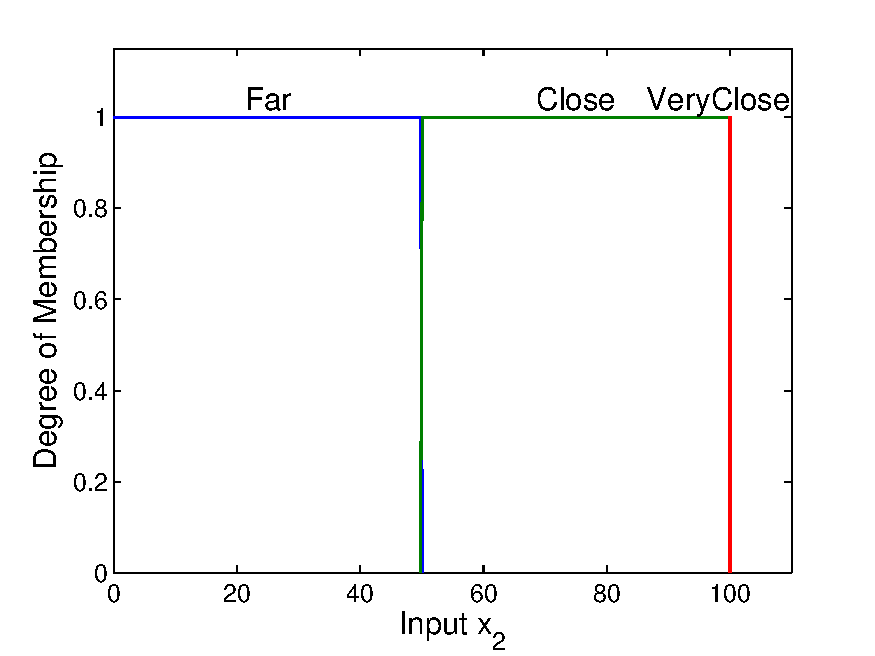
\includegraphics{images/x2_mfs.pdf}}
        %\subfigure[$x_2$ membership functions\label{f:x2mfs}]{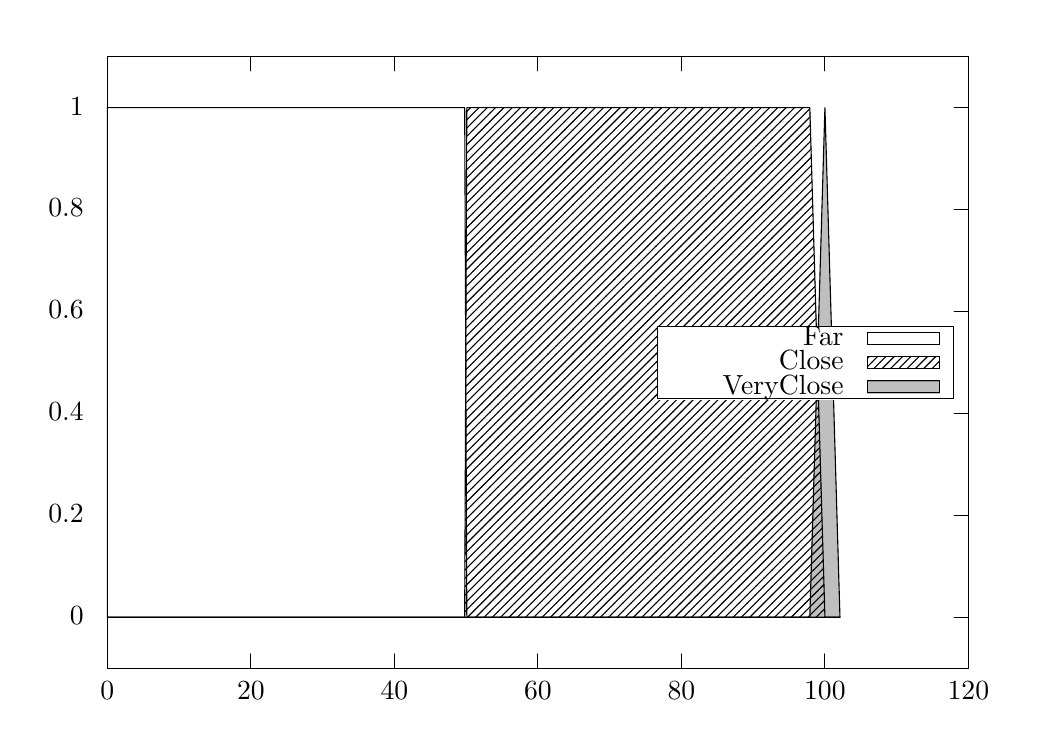
\begin{tikzpicture}[gnuplot]
%% generated with GNUPLOT 5.0p3 (Lua 5.1; terminal rev. 99, script rev. 100)
%% Wed 28 Mar 2018 10:34:02 PM EDT
\gpmonochromelines
\path (0.000,0.000) rectangle (12.500,8.750);
\gpcolor{color=gp lt color border}
\gpsetlinetype{gp lt border}
\gpsetdashtype{gp dt solid}
\gpsetlinewidth{1.00}
\draw[gp path] (1.012,1.263)--(1.192,1.263);
\draw[gp path] (11.947,1.263)--(11.767,1.263);
\node[gp node right] at (0.828,1.263) {$0$};
\draw[gp path] (1.012,2.557)--(1.192,2.557);
\draw[gp path] (11.947,2.557)--(11.767,2.557);
\node[gp node right] at (0.828,2.557) {$0.2$};
\draw[gp path] (1.012,3.851)--(1.192,3.851);
\draw[gp path] (11.947,3.851)--(11.767,3.851);
\node[gp node right] at (0.828,3.851) {$0.4$};
\draw[gp path] (1.012,5.146)--(1.192,5.146);
\draw[gp path] (11.947,5.146)--(11.767,5.146);
\node[gp node right] at (0.828,5.146) {$0.6$};
\draw[gp path] (1.012,6.440)--(1.192,6.440);
\draw[gp path] (11.947,6.440)--(11.767,6.440);
\node[gp node right] at (0.828,6.440) {$0.8$};
\draw[gp path] (1.012,7.734)--(1.192,7.734);
\draw[gp path] (11.947,7.734)--(11.767,7.734);
\node[gp node right] at (0.828,7.734) {$1$};
\draw[gp path] (1.012,0.616)--(1.012,0.796);
\draw[gp path] (1.012,8.381)--(1.012,8.201);
\node[gp node center] at (1.012,0.308) {$0$};
\draw[gp path] (2.835,0.616)--(2.835,0.796);
\draw[gp path] (2.835,8.381)--(2.835,8.201);
\node[gp node center] at (2.835,0.308) {$20$};
\draw[gp path] (4.657,0.616)--(4.657,0.796);
\draw[gp path] (4.657,8.381)--(4.657,8.201);
\node[gp node center] at (4.657,0.308) {$40$};
\draw[gp path] (6.480,0.616)--(6.480,0.796);
\draw[gp path] (6.480,8.381)--(6.480,8.201);
\node[gp node center] at (6.480,0.308) {$60$};
\draw[gp path] (8.302,0.616)--(8.302,0.796);
\draw[gp path] (8.302,8.381)--(8.302,8.201);
\node[gp node center] at (8.302,0.308) {$80$};
\draw[gp path] (10.125,0.616)--(10.125,0.796);
\draw[gp path] (10.125,8.381)--(10.125,8.201);
\node[gp node center] at (10.125,0.308) {$100$};
\draw[gp path] (11.947,0.616)--(11.947,0.796);
\draw[gp path] (11.947,8.381)--(11.947,8.201);
\node[gp node center] at (11.947,0.308) {$120$};
\draw[gp path] (1.012,8.381)--(1.012,0.616)--(11.947,0.616)--(11.947,8.381)--cycle;
\draw[gp path] (7.995,4.036)--(7.995,4.960)--(11.763,4.960)--(11.763,4.036)--cycle;
\gpfill{color=gp lt color border,gp pattern 0,pattern color=.} (1.012,1.263)--(1.012,7.734)--(5.550,7.734)--(5.577,1.263)%
    --(9.933,1.263)--(10.125,1.263)--(10.316,1.263)--cycle;
\draw[gp path] (1.012,1.263)--(1.012,7.734)--(5.550,7.734)--(5.577,1.263)--(9.933,1.263)%
  --(10.125,1.263)--(10.316,1.263);
\gpfill{color=gp lt color border,gp pattern 1,pattern color=.} (1.012,1.263)--(1.012,1.263)--(5.550,1.263)--(5.577,7.734)%
    --(9.933,7.734)--(10.125,1.263)--(10.316,1.263)--cycle;
\gpsetdashtype{gp dt 2}
\draw[gp path] (1.012,1.263)--(5.550,1.263)--(5.577,7.734)--(9.933,7.734)--(10.125,1.263)%
  --(10.316,1.263);
\gpfill{color=gp lt color border,opacity=0.25} (1.012,1.263)--(1.012,1.263)--(5.550,1.263)--(5.577,1.263)%
    --(9.933,1.263)--(10.125,7.734)--(10.316,1.263)--cycle;
\gpsetdashtype{gp dt 3}
\draw[gp path] (1.012,1.263)--(5.550,1.263)--(5.577,1.263)--(9.933,1.263)--(10.125,7.734)%
  --(10.316,1.263);
\gpfill{color=gpbgfillcolor} (7.995,4.036)--(11.763,4.036)--(11.763,4.960)--(7.995,4.960)--cycle;
\gpsetdashtype{gp dt solid}
\draw[gp path] (7.995,4.036)--(7.995,4.960)--(11.763,4.960)--(11.763,4.036)--cycle;
\node[gp node right] at (10.479,4.806) {Far};
\gpfill{color=gp lt color border,gp pattern 0,pattern color=.} (10.663,4.729)--(11.579,4.729)--(11.579,4.883)--(10.663,4.883)--cycle;
\draw[gp path] (10.663,4.729)--(11.579,4.729)--(11.579,4.883)--(10.663,4.883)--cycle;
\node[gp node right] at (10.479,4.498) {Close};
\gpfill{color=gp lt color border,gp pattern 1,pattern color=.} (10.663,4.421)--(11.579,4.421)--(11.579,4.575)--(10.663,4.575)--cycle;
\gpsetdashtype{gp dt 2}
\draw[gp path] (10.663,4.421)--(11.579,4.421)--(11.579,4.575)--(10.663,4.575)--cycle;
\node[gp node right] at (10.479,4.190) {VeryClose};
\gpfill{color=gp lt color border,opacity=0.25} (10.663,4.113)--(11.579,4.113)--(11.579,4.267)--(10.663,4.267)--cycle;
\gpsetdashtype{gp dt 3}
\draw[gp path] (10.663,4.113)--(11.579,4.113)--(11.579,4.267)--(10.663,4.267)--cycle;
\gpsetdashtype{gp dt solid}
\draw[gp path] (1.012,8.381)--(1.012,0.616)--(11.947,0.616)--(11.947,8.381)--cycle;
%% coordinates of the plot area
\gpdefrectangularnode{gp plot 1}{\pgfpoint{1.012cm}{0.616cm}}{\pgfpoint{11.947cm}{8.381cm}}
\end{tikzpicture}
%% gnuplot variables
}
        %%\subfigure[$\dot{x}_2$ membership functions\label{f:x4mfs}]{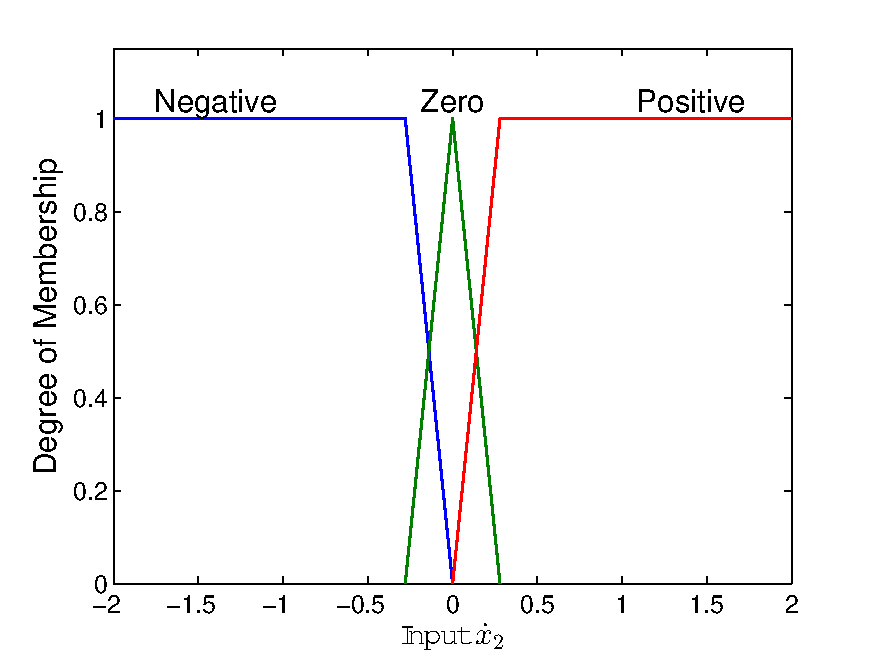
\includegraphics{images/x4_mfs.pdf}}
        %\subfigure[$\dot{x}_2$ membership functions\label{f:x4mfs}]{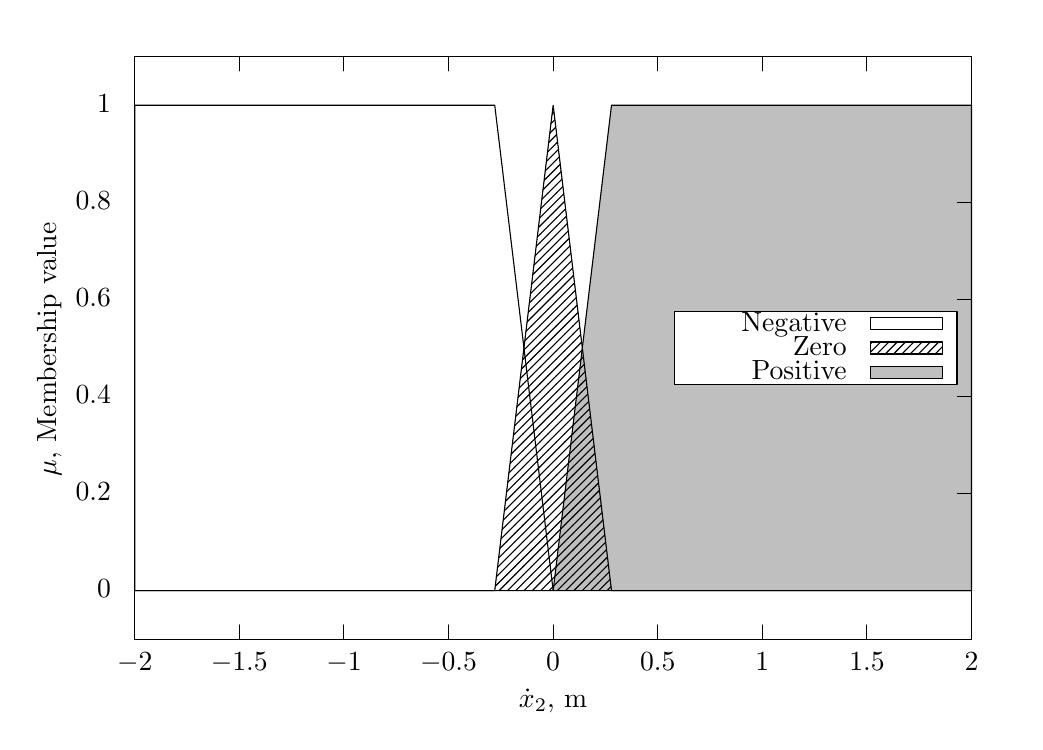
\begin{tikzpicture}[gnuplot]
%% generated with GNUPLOT 5.0p3 (Lua 5.1; terminal rev. 99, script rev. 100)
%% Wed 28 Mar 2018 10:34:02 PM EDT
\gpmonochromelines
\path (0.000,0.000) rectangle (12.500,8.750);
\gpcolor{color=gp lt color border}
\gpsetlinetype{gp lt border}
\gpsetdashtype{gp dt solid}
\gpsetlinewidth{1.00}
\draw[gp path] (1.320,1.601)--(1.500,1.601);
\draw[gp path] (11.947,1.601)--(11.767,1.601);
\node[gp node right] at (1.136,1.601) {$0$};
\draw[gp path] (1.320,2.834)--(1.500,2.834);
\draw[gp path] (11.947,2.834)--(11.767,2.834);
\node[gp node right] at (1.136,2.834) {$0.2$};
\draw[gp path] (1.320,4.067)--(1.500,4.067);
\draw[gp path] (11.947,4.067)--(11.767,4.067);
\node[gp node right] at (1.136,4.067) {$0.4$};
\draw[gp path] (1.320,5.299)--(1.500,5.299);
\draw[gp path] (11.947,5.299)--(11.767,5.299);
\node[gp node right] at (1.136,5.299) {$0.6$};
\draw[gp path] (1.320,6.532)--(1.500,6.532);
\draw[gp path] (11.947,6.532)--(11.767,6.532);
\node[gp node right] at (1.136,6.532) {$0.8$};
\draw[gp path] (1.320,7.765)--(1.500,7.765);
\draw[gp path] (11.947,7.765)--(11.767,7.765);
\node[gp node right] at (1.136,7.765) {$1$};
\draw[gp path] (1.320,0.985)--(1.320,1.165);
\draw[gp path] (1.320,8.381)--(1.320,8.201);
\node[gp node center] at (1.320,0.677) {$-2$};
\draw[gp path] (2.648,0.985)--(2.648,1.165);
\draw[gp path] (2.648,8.381)--(2.648,8.201);
\node[gp node center] at (2.648,0.677) {$-1.5$};
\draw[gp path] (3.977,0.985)--(3.977,1.165);
\draw[gp path] (3.977,8.381)--(3.977,8.201);
\node[gp node center] at (3.977,0.677) {$-1$};
\draw[gp path] (5.305,0.985)--(5.305,1.165);
\draw[gp path] (5.305,8.381)--(5.305,8.201);
\node[gp node center] at (5.305,0.677) {$-0.5$};
\draw[gp path] (6.634,0.985)--(6.634,1.165);
\draw[gp path] (6.634,8.381)--(6.634,8.201);
\node[gp node center] at (6.634,0.677) {$0$};
\draw[gp path] (7.962,0.985)--(7.962,1.165);
\draw[gp path] (7.962,8.381)--(7.962,8.201);
\node[gp node center] at (7.962,0.677) {$0.5$};
\draw[gp path] (9.290,0.985)--(9.290,1.165);
\draw[gp path] (9.290,8.381)--(9.290,8.201);
\node[gp node center] at (9.290,0.677) {$1$};
\draw[gp path] (10.619,0.985)--(10.619,1.165);
\draw[gp path] (10.619,8.381)--(10.619,8.201);
\node[gp node center] at (10.619,0.677) {$1.5$};
\draw[gp path] (11.947,0.985)--(11.947,1.165);
\draw[gp path] (11.947,8.381)--(11.947,8.201);
\node[gp node center] at (11.947,0.677) {$2$};
\draw[gp path] (1.320,8.381)--(1.320,0.985)--(11.947,0.985)--(11.947,8.381)--cycle;
\node[gp node center,rotate=-270] at (0.246,4.683) {$\mu$, Membership value};
\node[gp node center] at (6.633,0.215) {$\dot{x}_2$, m};
\draw[gp path] (8.179,4.221)--(8.179,5.145)--(11.763,5.145)--(11.763,4.221)--cycle;
\gpfill{color=gp lt color border,gp pattern 0,pattern color=.} (1.320,1.601)--(1.320,7.765)--(5.892,7.765)--(6.634,1.601)%
    --(7.375,1.601)--(11.947,1.601)--(11.947,1.601)--cycle;
\draw[gp path] (1.320,1.601)--(1.320,7.765)--(5.892,7.765)--(6.634,1.601)--(7.375,1.601)%
  --(11.947,1.601);
\gpfill{color=gp lt color border,gp pattern 1,pattern color=.} (1.320,1.601)--(1.320,1.601)--(5.892,1.601)--(6.634,7.765)%
    --(7.375,1.601)--(11.947,1.601)--(11.947,1.601)--cycle;
\gpsetdashtype{gp dt 2}
\draw[gp path] (1.320,1.601)--(5.892,1.601)--(6.634,7.765)--(7.375,1.601)--(11.947,1.601);
\gpfill{color=gp lt color border,opacity=0.25} (1.320,1.601)--(1.320,1.601)--(5.892,1.601)--(6.634,1.601)%
    --(7.375,7.765)--(11.947,7.765)--(11.947,1.601)--cycle;
\gpsetdashtype{gp dt 3}
\draw[gp path] (1.320,1.601)--(5.892,1.601)--(6.634,1.601)--(7.375,7.765)--(11.947,7.765)%
  --(11.947,1.601);
\gpfill{color=gpbgfillcolor} (8.179,4.221)--(11.763,4.221)--(11.763,5.145)--(8.179,5.145)--cycle;
\gpsetdashtype{gp dt solid}
\draw[gp path] (8.179,4.221)--(8.179,5.145)--(11.763,5.145)--(11.763,4.221)--cycle;
\node[gp node right] at (10.479,4.991) {Negative};
\gpfill{color=gp lt color border,gp pattern 0,pattern color=.} (10.663,4.914)--(11.579,4.914)--(11.579,5.068)--(10.663,5.068)--cycle;
\draw[gp path] (10.663,4.914)--(11.579,4.914)--(11.579,5.068)--(10.663,5.068)--cycle;
\node[gp node right] at (10.479,4.683) {Zero};
\gpfill{color=gp lt color border,gp pattern 1,pattern color=.} (10.663,4.606)--(11.579,4.606)--(11.579,4.760)--(10.663,4.760)--cycle;
\gpsetdashtype{gp dt 2}
\draw[gp path] (10.663,4.606)--(11.579,4.606)--(11.579,4.760)--(10.663,4.760)--cycle;
\node[gp node right] at (10.479,4.375) {Positive};
\gpfill{color=gp lt color border,opacity=0.25} (10.663,4.298)--(11.579,4.298)--(11.579,4.452)--(10.663,4.452)--cycle;
\gpsetdashtype{gp dt 3}
\draw[gp path] (10.663,4.298)--(11.579,4.298)--(11.579,4.452)--(10.663,4.452)--cycle;
\gpsetdashtype{gp dt solid}
\draw[gp path] (1.320,8.381)--(1.320,0.985)--(11.947,0.985)--(11.947,8.381)--cycle;
%% coordinates of the plot area
\gpdefrectangularnode{gp plot 1}{\pgfpoint{1.320cm}{0.985cm}}{\pgfpoint{11.947cm}{8.381cm}}
\end{tikzpicture}
%% gnuplot variables
}
    %\end{subfigmatrix} \caption{Input membership functions}\label{f:mfs}
%\end{figure}

\begin{figure}[ht]
    \centering
    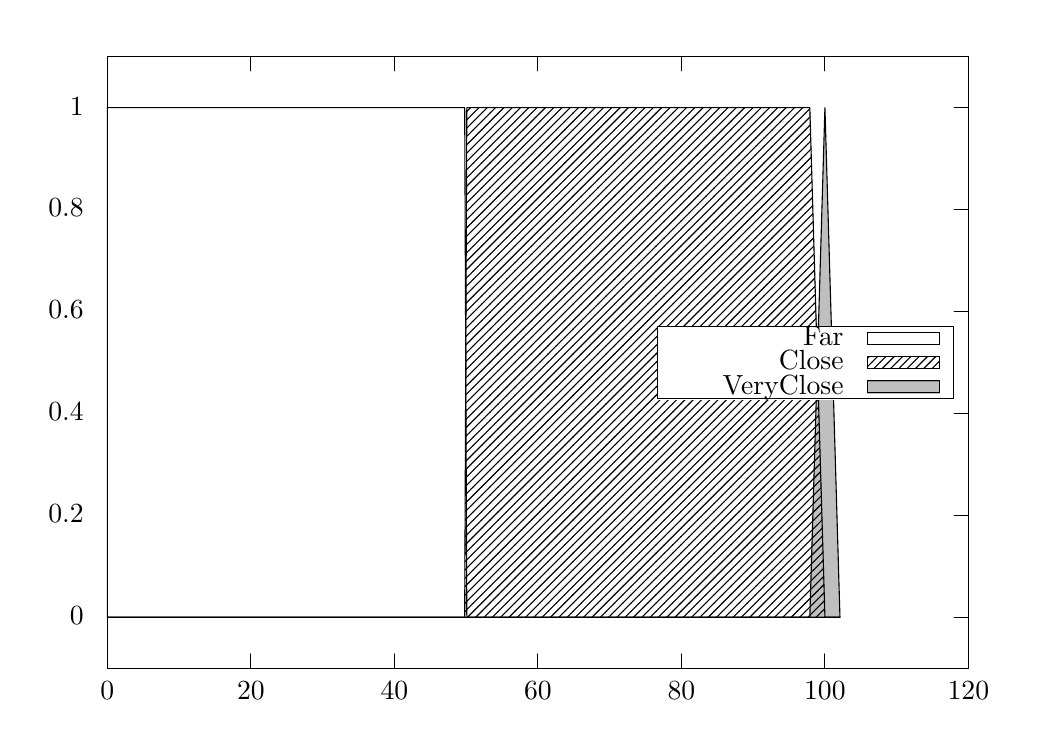
\begin{tikzpicture}[gnuplot]
%% generated with GNUPLOT 5.0p3 (Lua 5.1; terminal rev. 99, script rev. 100)
%% Wed 28 Mar 2018 10:34:02 PM EDT
\gpmonochromelines
\path (0.000,0.000) rectangle (12.500,8.750);
\gpcolor{color=gp lt color border}
\gpsetlinetype{gp lt border}
\gpsetdashtype{gp dt solid}
\gpsetlinewidth{1.00}
\draw[gp path] (1.012,1.263)--(1.192,1.263);
\draw[gp path] (11.947,1.263)--(11.767,1.263);
\node[gp node right] at (0.828,1.263) {$0$};
\draw[gp path] (1.012,2.557)--(1.192,2.557);
\draw[gp path] (11.947,2.557)--(11.767,2.557);
\node[gp node right] at (0.828,2.557) {$0.2$};
\draw[gp path] (1.012,3.851)--(1.192,3.851);
\draw[gp path] (11.947,3.851)--(11.767,3.851);
\node[gp node right] at (0.828,3.851) {$0.4$};
\draw[gp path] (1.012,5.146)--(1.192,5.146);
\draw[gp path] (11.947,5.146)--(11.767,5.146);
\node[gp node right] at (0.828,5.146) {$0.6$};
\draw[gp path] (1.012,6.440)--(1.192,6.440);
\draw[gp path] (11.947,6.440)--(11.767,6.440);
\node[gp node right] at (0.828,6.440) {$0.8$};
\draw[gp path] (1.012,7.734)--(1.192,7.734);
\draw[gp path] (11.947,7.734)--(11.767,7.734);
\node[gp node right] at (0.828,7.734) {$1$};
\draw[gp path] (1.012,0.616)--(1.012,0.796);
\draw[gp path] (1.012,8.381)--(1.012,8.201);
\node[gp node center] at (1.012,0.308) {$0$};
\draw[gp path] (2.835,0.616)--(2.835,0.796);
\draw[gp path] (2.835,8.381)--(2.835,8.201);
\node[gp node center] at (2.835,0.308) {$20$};
\draw[gp path] (4.657,0.616)--(4.657,0.796);
\draw[gp path] (4.657,8.381)--(4.657,8.201);
\node[gp node center] at (4.657,0.308) {$40$};
\draw[gp path] (6.480,0.616)--(6.480,0.796);
\draw[gp path] (6.480,8.381)--(6.480,8.201);
\node[gp node center] at (6.480,0.308) {$60$};
\draw[gp path] (8.302,0.616)--(8.302,0.796);
\draw[gp path] (8.302,8.381)--(8.302,8.201);
\node[gp node center] at (8.302,0.308) {$80$};
\draw[gp path] (10.125,0.616)--(10.125,0.796);
\draw[gp path] (10.125,8.381)--(10.125,8.201);
\node[gp node center] at (10.125,0.308) {$100$};
\draw[gp path] (11.947,0.616)--(11.947,0.796);
\draw[gp path] (11.947,8.381)--(11.947,8.201);
\node[gp node center] at (11.947,0.308) {$120$};
\draw[gp path] (1.012,8.381)--(1.012,0.616)--(11.947,0.616)--(11.947,8.381)--cycle;
\draw[gp path] (7.995,4.036)--(7.995,4.960)--(11.763,4.960)--(11.763,4.036)--cycle;
\gpfill{color=gp lt color border,gp pattern 0,pattern color=.} (1.012,1.263)--(1.012,7.734)--(5.550,7.734)--(5.577,1.263)%
    --(9.933,1.263)--(10.125,1.263)--(10.316,1.263)--cycle;
\draw[gp path] (1.012,1.263)--(1.012,7.734)--(5.550,7.734)--(5.577,1.263)--(9.933,1.263)%
  --(10.125,1.263)--(10.316,1.263);
\gpfill{color=gp lt color border,gp pattern 1,pattern color=.} (1.012,1.263)--(1.012,1.263)--(5.550,1.263)--(5.577,7.734)%
    --(9.933,7.734)--(10.125,1.263)--(10.316,1.263)--cycle;
\gpsetdashtype{gp dt 2}
\draw[gp path] (1.012,1.263)--(5.550,1.263)--(5.577,7.734)--(9.933,7.734)--(10.125,1.263)%
  --(10.316,1.263);
\gpfill{color=gp lt color border,opacity=0.25} (1.012,1.263)--(1.012,1.263)--(5.550,1.263)--(5.577,1.263)%
    --(9.933,1.263)--(10.125,7.734)--(10.316,1.263)--cycle;
\gpsetdashtype{gp dt 3}
\draw[gp path] (1.012,1.263)--(5.550,1.263)--(5.577,1.263)--(9.933,1.263)--(10.125,7.734)%
  --(10.316,1.263);
\gpfill{color=gpbgfillcolor} (7.995,4.036)--(11.763,4.036)--(11.763,4.960)--(7.995,4.960)--cycle;
\gpsetdashtype{gp dt solid}
\draw[gp path] (7.995,4.036)--(7.995,4.960)--(11.763,4.960)--(11.763,4.036)--cycle;
\node[gp node right] at (10.479,4.806) {Far};
\gpfill{color=gp lt color border,gp pattern 0,pattern color=.} (10.663,4.729)--(11.579,4.729)--(11.579,4.883)--(10.663,4.883)--cycle;
\draw[gp path] (10.663,4.729)--(11.579,4.729)--(11.579,4.883)--(10.663,4.883)--cycle;
\node[gp node right] at (10.479,4.498) {Close};
\gpfill{color=gp lt color border,gp pattern 1,pattern color=.} (10.663,4.421)--(11.579,4.421)--(11.579,4.575)--(10.663,4.575)--cycle;
\gpsetdashtype{gp dt 2}
\draw[gp path] (10.663,4.421)--(11.579,4.421)--(11.579,4.575)--(10.663,4.575)--cycle;
\node[gp node right] at (10.479,4.190) {VeryClose};
\gpfill{color=gp lt color border,opacity=0.25} (10.663,4.113)--(11.579,4.113)--(11.579,4.267)--(10.663,4.267)--cycle;
\gpsetdashtype{gp dt 3}
\draw[gp path] (10.663,4.113)--(11.579,4.113)--(11.579,4.267)--(10.663,4.267)--cycle;
\gpsetdashtype{gp dt solid}
\draw[gp path] (1.012,8.381)--(1.012,0.616)--(11.947,0.616)--(11.947,8.381)--cycle;
%% coordinates of the plot area
\gpdefrectangularnode{gp plot 1}{\pgfpoint{1.012cm}{0.616cm}}{\pgfpoint{11.947cm}{8.381cm}}
\end{tikzpicture}
%% gnuplot variables

    \caption{$x_2$ membership functions}\label{f:x2mfs}
\end{figure}

\begin{figure}[ht]
    \centering
    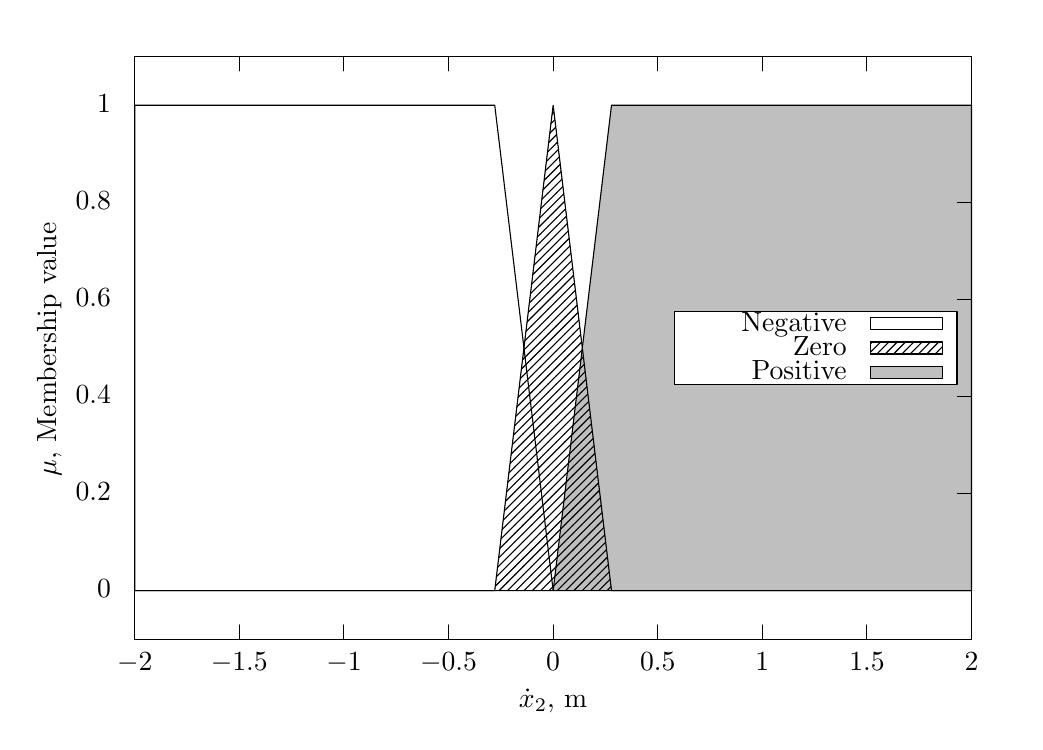
\begin{tikzpicture}[gnuplot]
%% generated with GNUPLOT 5.0p3 (Lua 5.1; terminal rev. 99, script rev. 100)
%% Wed 28 Mar 2018 10:34:02 PM EDT
\gpmonochromelines
\path (0.000,0.000) rectangle (12.500,8.750);
\gpcolor{color=gp lt color border}
\gpsetlinetype{gp lt border}
\gpsetdashtype{gp dt solid}
\gpsetlinewidth{1.00}
\draw[gp path] (1.320,1.601)--(1.500,1.601);
\draw[gp path] (11.947,1.601)--(11.767,1.601);
\node[gp node right] at (1.136,1.601) {$0$};
\draw[gp path] (1.320,2.834)--(1.500,2.834);
\draw[gp path] (11.947,2.834)--(11.767,2.834);
\node[gp node right] at (1.136,2.834) {$0.2$};
\draw[gp path] (1.320,4.067)--(1.500,4.067);
\draw[gp path] (11.947,4.067)--(11.767,4.067);
\node[gp node right] at (1.136,4.067) {$0.4$};
\draw[gp path] (1.320,5.299)--(1.500,5.299);
\draw[gp path] (11.947,5.299)--(11.767,5.299);
\node[gp node right] at (1.136,5.299) {$0.6$};
\draw[gp path] (1.320,6.532)--(1.500,6.532);
\draw[gp path] (11.947,6.532)--(11.767,6.532);
\node[gp node right] at (1.136,6.532) {$0.8$};
\draw[gp path] (1.320,7.765)--(1.500,7.765);
\draw[gp path] (11.947,7.765)--(11.767,7.765);
\node[gp node right] at (1.136,7.765) {$1$};
\draw[gp path] (1.320,0.985)--(1.320,1.165);
\draw[gp path] (1.320,8.381)--(1.320,8.201);
\node[gp node center] at (1.320,0.677) {$-2$};
\draw[gp path] (2.648,0.985)--(2.648,1.165);
\draw[gp path] (2.648,8.381)--(2.648,8.201);
\node[gp node center] at (2.648,0.677) {$-1.5$};
\draw[gp path] (3.977,0.985)--(3.977,1.165);
\draw[gp path] (3.977,8.381)--(3.977,8.201);
\node[gp node center] at (3.977,0.677) {$-1$};
\draw[gp path] (5.305,0.985)--(5.305,1.165);
\draw[gp path] (5.305,8.381)--(5.305,8.201);
\node[gp node center] at (5.305,0.677) {$-0.5$};
\draw[gp path] (6.634,0.985)--(6.634,1.165);
\draw[gp path] (6.634,8.381)--(6.634,8.201);
\node[gp node center] at (6.634,0.677) {$0$};
\draw[gp path] (7.962,0.985)--(7.962,1.165);
\draw[gp path] (7.962,8.381)--(7.962,8.201);
\node[gp node center] at (7.962,0.677) {$0.5$};
\draw[gp path] (9.290,0.985)--(9.290,1.165);
\draw[gp path] (9.290,8.381)--(9.290,8.201);
\node[gp node center] at (9.290,0.677) {$1$};
\draw[gp path] (10.619,0.985)--(10.619,1.165);
\draw[gp path] (10.619,8.381)--(10.619,8.201);
\node[gp node center] at (10.619,0.677) {$1.5$};
\draw[gp path] (11.947,0.985)--(11.947,1.165);
\draw[gp path] (11.947,8.381)--(11.947,8.201);
\node[gp node center] at (11.947,0.677) {$2$};
\draw[gp path] (1.320,8.381)--(1.320,0.985)--(11.947,0.985)--(11.947,8.381)--cycle;
\node[gp node center,rotate=-270] at (0.246,4.683) {$\mu$, Membership value};
\node[gp node center] at (6.633,0.215) {$\dot{x}_2$, m};
\draw[gp path] (8.179,4.221)--(8.179,5.145)--(11.763,5.145)--(11.763,4.221)--cycle;
\gpfill{color=gp lt color border,gp pattern 0,pattern color=.} (1.320,1.601)--(1.320,7.765)--(5.892,7.765)--(6.634,1.601)%
    --(7.375,1.601)--(11.947,1.601)--(11.947,1.601)--cycle;
\draw[gp path] (1.320,1.601)--(1.320,7.765)--(5.892,7.765)--(6.634,1.601)--(7.375,1.601)%
  --(11.947,1.601);
\gpfill{color=gp lt color border,gp pattern 1,pattern color=.} (1.320,1.601)--(1.320,1.601)--(5.892,1.601)--(6.634,7.765)%
    --(7.375,1.601)--(11.947,1.601)--(11.947,1.601)--cycle;
\gpsetdashtype{gp dt 2}
\draw[gp path] (1.320,1.601)--(5.892,1.601)--(6.634,7.765)--(7.375,1.601)--(11.947,1.601);
\gpfill{color=gp lt color border,opacity=0.25} (1.320,1.601)--(1.320,1.601)--(5.892,1.601)--(6.634,1.601)%
    --(7.375,7.765)--(11.947,7.765)--(11.947,1.601)--cycle;
\gpsetdashtype{gp dt 3}
\draw[gp path] (1.320,1.601)--(5.892,1.601)--(6.634,1.601)--(7.375,7.765)--(11.947,7.765)%
  --(11.947,1.601);
\gpfill{color=gpbgfillcolor} (8.179,4.221)--(11.763,4.221)--(11.763,5.145)--(8.179,5.145)--cycle;
\gpsetdashtype{gp dt solid}
\draw[gp path] (8.179,4.221)--(8.179,5.145)--(11.763,5.145)--(11.763,4.221)--cycle;
\node[gp node right] at (10.479,4.991) {Negative};
\gpfill{color=gp lt color border,gp pattern 0,pattern color=.} (10.663,4.914)--(11.579,4.914)--(11.579,5.068)--(10.663,5.068)--cycle;
\draw[gp path] (10.663,4.914)--(11.579,4.914)--(11.579,5.068)--(10.663,5.068)--cycle;
\node[gp node right] at (10.479,4.683) {Zero};
\gpfill{color=gp lt color border,gp pattern 1,pattern color=.} (10.663,4.606)--(11.579,4.606)--(11.579,4.760)--(10.663,4.760)--cycle;
\gpsetdashtype{gp dt 2}
\draw[gp path] (10.663,4.606)--(11.579,4.606)--(11.579,4.760)--(10.663,4.760)--cycle;
\node[gp node right] at (10.479,4.375) {Positive};
\gpfill{color=gp lt color border,opacity=0.25} (10.663,4.298)--(11.579,4.298)--(11.579,4.452)--(10.663,4.452)--cycle;
\gpsetdashtype{gp dt 3}
\draw[gp path] (10.663,4.298)--(11.579,4.298)--(11.579,4.452)--(10.663,4.452)--cycle;
\gpsetdashtype{gp dt solid}
\draw[gp path] (1.320,8.381)--(1.320,0.985)--(11.947,0.985)--(11.947,8.381)--cycle;
%% coordinates of the plot area
\gpdefrectangularnode{gp plot 1}{\pgfpoint{1.320cm}{0.985cm}}{\pgfpoint{11.947cm}{8.381cm}}
\end{tikzpicture}
%% gnuplot variables

    \caption{$\dot{x}_2$ membership functions}\label{f:x4mfs}
\end{figure}


The velocity membership function parameters are: \begin{displaymath} \mathrm{Negative:}\quad
\begin{bmatrix}
\SI{-6}{\metre\per\second}\\\SI{-6}{\metre\per\second}\\\SI{-.2792}{\metre\per\second}\\\SI{0}{\metre\per\second}
\end{bmatrix}, \quad \mathrm{Zero:}\quad \begin{bmatrix}
    \SI{-0.2792}{\metre\per\second}\\\SI{0}{\metre\per\second}\\\SI{0.2792}{\metre\per\second} \end{bmatrix},
\end{displaymath} \begin{displaymath} \mathrm{Positive:}\quad \begin{bmatrix}
\SI{0}{\metre\per\second}\\\SI{0.2792}{\metre\per\second}\\\SI{6}{\metre\per\second}\\\SI{6}{\metre\per\second}
\end{bmatrix} \end{displaymath}
\subsubsection{Rule Base}\label{ss:rulebase}
As previously discussed, the rule base of an FIS is a series of IF-THEN (antecedent-consequent) conditions
that use the membership functions of all the inputs in order to determine the output variable. There are also
several membership functions for the output variable that the rule base maps to. Each of the rules has an
influence on what the output of the system should be. The weight of these influences again varies from 0 to 1
and the final output value is determined by calculating the centroid of all of the rules. For instance, one
rule dictates that if the car is far away then the output force should be positive and large so that the car
will move towards the wall. Another rule will say that when the car is close to the wall the output force
should be negative in order to slow the car down. All of these rules have influence over all input ranges
determined by how the input variables map to the given membership functions in that specific rule.

The antecedent of each statement contains memberships of both input variables and the consequent maps to the
output membership functions. The rules for this FIS were developed based upon intuitive decision making. The
rules developed for our FIS are shown in \cref{tab:rulebase}.  
\begin{table}[ht]
    \begin{center}
        \caption{Rule Base of the Fuzzy Inference System}\label{tab:rulebase}
        \begin{tabular}{ccccc} \multicolumn{2}{c}{}  & \multicolumn{3}{c}{Velocity Measurement}\\ \cline{3-5}
            \multicolumn{2}{c|}{}  & \multicolumn{1}{c|}{\textbf{Negative}} & \multicolumn{1}{c|}{\textbf{Zero}} & \multicolumn{1}{c|}{\textbf{Positive}} \\ \cline{2-5}
            \multicolumn{1}{c|}{\multirow{3}{*}{\parbox{3cm}{\centering Position\\Measurement}}} & \multicolumn{1}{c|}{\textbf{Far}} & \multicolumn{3}{c|}{Positive} \\ \cline{2-5}
            \multicolumn{1}{c|}{} & \multicolumn{1}{c|}{\textbf{Close}} & \multicolumn{1}{c|}{Positive} & \multicolumn{1}{c|}{Zero} & \multicolumn{1}{c|}{Negative}\\\cline{2-5}
            \multicolumn{1}{c|}{} & \multicolumn{1}{c|}{\textbf{VeryClose}} & \multicolumn{1}{c|}{Positive} & \multicolumn{1}{c|}{Zero} & \multicolumn{1}{c|}{Negative} \\ \cline{2-5}
            \multicolumn{2}{c}{}  & \multicolumn{3}{c}{Control Force}
        \end{tabular}
    \end{center}
\end{table}

\subsubsection{Control Force}
\begin{figure}[ht]
    \centering
    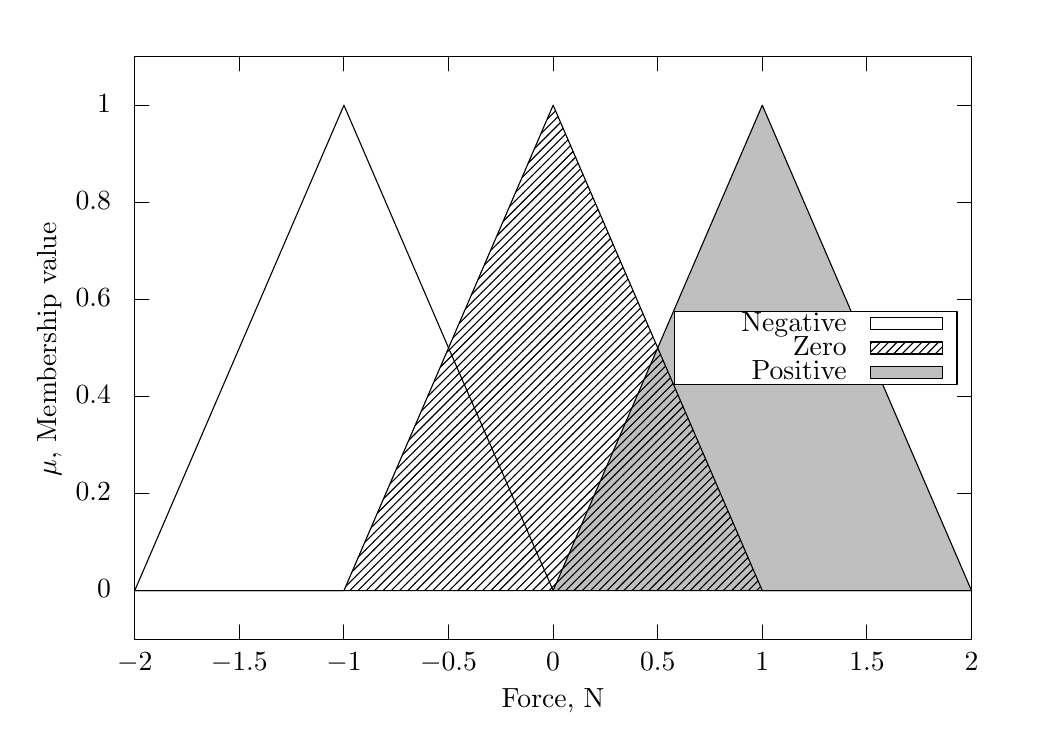
\begin{tikzpicture}[gnuplot]
%% generated with GNUPLOT 5.0p3 (Lua 5.1; terminal rev. 99, script rev. 100)
%% Wed 28 Mar 2018 10:34:02 PM EDT
\gpmonochromelines
\path (0.000,0.000) rectangle (12.500,8.750);
\gpcolor{color=gp lt color border}
\gpsetlinetype{gp lt border}
\gpsetdashtype{gp dt solid}
\gpsetlinewidth{1.00}
\draw[gp path] (1.320,1.601)--(1.500,1.601);
\draw[gp path] (11.947,1.601)--(11.767,1.601);
\node[gp node right] at (1.136,1.601) {$0$};
\draw[gp path] (1.320,2.834)--(1.500,2.834);
\draw[gp path] (11.947,2.834)--(11.767,2.834);
\node[gp node right] at (1.136,2.834) {$0.2$};
\draw[gp path] (1.320,4.067)--(1.500,4.067);
\draw[gp path] (11.947,4.067)--(11.767,4.067);
\node[gp node right] at (1.136,4.067) {$0.4$};
\draw[gp path] (1.320,5.299)--(1.500,5.299);
\draw[gp path] (11.947,5.299)--(11.767,5.299);
\node[gp node right] at (1.136,5.299) {$0.6$};
\draw[gp path] (1.320,6.532)--(1.500,6.532);
\draw[gp path] (11.947,6.532)--(11.767,6.532);
\node[gp node right] at (1.136,6.532) {$0.8$};
\draw[gp path] (1.320,7.765)--(1.500,7.765);
\draw[gp path] (11.947,7.765)--(11.767,7.765);
\node[gp node right] at (1.136,7.765) {$1$};
\draw[gp path] (1.320,0.985)--(1.320,1.165);
\draw[gp path] (1.320,8.381)--(1.320,8.201);
\node[gp node center] at (1.320,0.677) {$-2$};
\draw[gp path] (2.648,0.985)--(2.648,1.165);
\draw[gp path] (2.648,8.381)--(2.648,8.201);
\node[gp node center] at (2.648,0.677) {$-1.5$};
\draw[gp path] (3.977,0.985)--(3.977,1.165);
\draw[gp path] (3.977,8.381)--(3.977,8.201);
\node[gp node center] at (3.977,0.677) {$-1$};
\draw[gp path] (5.305,0.985)--(5.305,1.165);
\draw[gp path] (5.305,8.381)--(5.305,8.201);
\node[gp node center] at (5.305,0.677) {$-0.5$};
\draw[gp path] (6.634,0.985)--(6.634,1.165);
\draw[gp path] (6.634,8.381)--(6.634,8.201);
\node[gp node center] at (6.634,0.677) {$0$};
\draw[gp path] (7.962,0.985)--(7.962,1.165);
\draw[gp path] (7.962,8.381)--(7.962,8.201);
\node[gp node center] at (7.962,0.677) {$0.5$};
\draw[gp path] (9.290,0.985)--(9.290,1.165);
\draw[gp path] (9.290,8.381)--(9.290,8.201);
\node[gp node center] at (9.290,0.677) {$1$};
\draw[gp path] (10.619,0.985)--(10.619,1.165);
\draw[gp path] (10.619,8.381)--(10.619,8.201);
\node[gp node center] at (10.619,0.677) {$1.5$};
\draw[gp path] (11.947,0.985)--(11.947,1.165);
\draw[gp path] (11.947,8.381)--(11.947,8.201);
\node[gp node center] at (11.947,0.677) {$2$};
\draw[gp path] (1.320,8.381)--(1.320,0.985)--(11.947,0.985)--(11.947,8.381)--cycle;
\node[gp node center,rotate=-270] at (0.246,4.683) {$\mu$, Membership value};
\node[gp node center] at (6.633,0.215) {Force, N};
\draw[gp path] (8.179,4.221)--(8.179,5.145)--(11.763,5.145)--(11.763,4.221)--cycle;
%
  \gpfill{color=gp lt color border,gp pattern 0,pattern color=.} (1.320,1.601)--(3.977,7.765)--(6.634,1.601)--(9.290,1.601)--(11.947,1.601)--cycle;
\draw[gp path] (1.320,1.601)--(3.977,7.765)--(6.634,1.601)--(9.290,1.601)--(11.947,1.601);
%
  \gpfill{color=gp lt color border,gp pattern 1,pattern color=.} (1.320,1.601)--(3.977,1.601)--(6.634,7.765)--(9.290,1.601)--(11.947,1.601)--cycle;
\gpsetdashtype{gp dt 2}
\draw[gp path] (1.320,1.601)--(3.977,1.601)--(6.634,7.765)--(9.290,1.601)--(11.947,1.601);
%
  \gpfill{color=gp lt color border,opacity=0.25} (1.320,1.601)--(3.977,1.601)--(6.634,1.601)--(9.290,7.765)--(11.947,1.601)--cycle;
\gpsetdashtype{gp dt 3}
\draw[gp path] (1.320,1.601)--(3.977,1.601)--(6.634,1.601)--(9.290,7.765)--(11.947,1.601);
\gpfill{color=gpbgfillcolor} (8.179,4.221)--(11.763,4.221)--(11.763,5.145)--(8.179,5.145)--cycle;
\gpsetdashtype{gp dt solid}
\draw[gp path] (8.179,4.221)--(8.179,5.145)--(11.763,5.145)--(11.763,4.221)--cycle;
\node[gp node right] at (10.479,4.991) {Negative};
\gpfill{color=gp lt color border,gp pattern 0,pattern color=.} (10.663,4.914)--(11.579,4.914)--(11.579,5.068)--(10.663,5.068)--cycle;
\draw[gp path] (10.663,4.914)--(11.579,4.914)--(11.579,5.068)--(10.663,5.068)--cycle;
\node[gp node right] at (10.479,4.683) {Zero};
\gpfill{color=gp lt color border,gp pattern 1,pattern color=.} (10.663,4.606)--(11.579,4.606)--(11.579,4.760)--(10.663,4.760)--cycle;
\gpsetdashtype{gp dt 2}
\draw[gp path] (10.663,4.606)--(11.579,4.606)--(11.579,4.760)--(10.663,4.760)--cycle;
\node[gp node right] at (10.479,4.375) {Positive};
\gpfill{color=gp lt color border,opacity=0.25} (10.663,4.298)--(11.579,4.298)--(11.579,4.452)--(10.663,4.452)--cycle;
\gpsetdashtype{gp dt 3}
\draw[gp path] (10.663,4.298)--(11.579,4.298)--(11.579,4.452)--(10.663,4.452)--cycle;
\gpsetdashtype{gp dt solid}
\draw[gp path] (1.320,8.381)--(1.320,0.985)--(11.947,0.985)--(11.947,8.381)--cycle;
%% coordinates of the plot area
\gpdefrectangularnode{gp plot 1}{\pgfpoint{1.320cm}{0.985cm}}{\pgfpoint{11.947cm}{8.381cm}}
\end{tikzpicture}
%% gnuplot variables

    \caption{Control force membership functions.}
    \label{f:fmfs}
\end{figure}
The output variable, force, is
also composed of three membership functions. The output force is bounded from \SIrange{-1}{1}{\newton} thus
the membership functions allow for the output to be ``Negative'', ``Zero'', or ``Positive''. As the centroid
of the area beneath each function is used to evaluate the control force, the upper and lower bounds are
centered over 1 and -1 respectively. These functions represent the ``defuzzification'' stage of the FIS and
these outputs are determined by evaluating each rule in the rule base (see \cref{ss:rulebase}) in
parallel\cite{matlab:12tb}. The controller emulates bang-bang control for the majority of the simulation
lifetime, sharply transitioning from full acceleration to full deceleration. As the cart system nears the
wall, the oscillation damping rules will dictate the force to apply on the system. Typically, the output force
will be directed opposite to the velocity of cart 2. The membership functions for the control force are shown
in \cref{f:fmfs}.
	
	
\begin{displaymath}
    \mathrm{Negative:}\quad 
        \begin{bmatrix}
            \SI{-2}{\newton}\\
            \SI{-1}{\newton}\\
            \SI{0}{\newton}
        \end{bmatrix}, \quad
    \mathrm{Zero:}\quad 
        \begin{bmatrix}
            \SI{-1}{\newton}\\
            \SI{0}{\newton}\\
            \SI{1}{\newton}
        \end{bmatrix}
\end{displaymath}
\begin{displaymath}
    \mathrm{Positive:}
    \quad 
        \begin{bmatrix}
            \SI{0}{\newton}\\
            \SI{1}{\newton}\\
            \SI{2}{\newton}
        \end{bmatrix}
\end{displaymath}

\subsection{Simulation Performance}\label{ss:simperf}
\begin{figure}[ht]
    \centering
    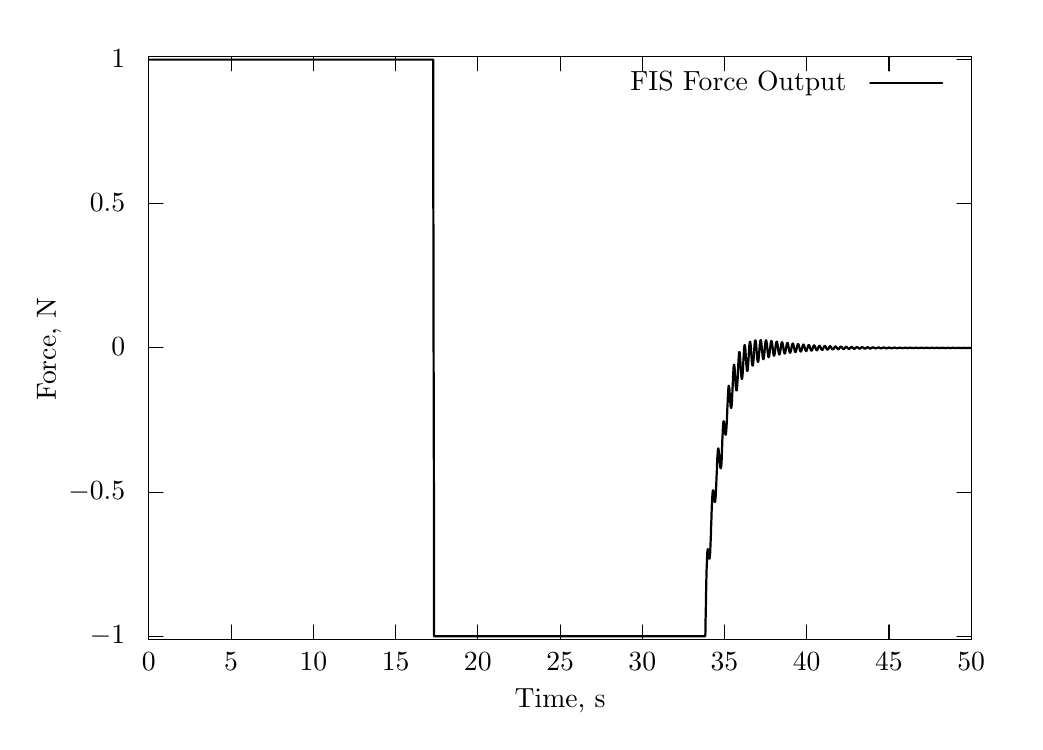
\begin{tikzpicture}[gnuplot]
%% generated with GNUPLOT 5.0p3 (Lua 5.1; terminal rev. 99, script rev. 100)
%% Thu 29 Mar 2018 12:41:19 AM EDT
\gpmonochromelines
\path (0.000,0.000) rectangle (12.500,8.750);
\gpcolor{color=gp lt color border}
\gpsetlinetype{gp lt border}
\gpsetdashtype{gp dt solid}
\gpsetlinewidth{1.00}
\draw[gp path] (1.504,1.022)--(1.684,1.022);
\draw[gp path] (11.947,1.022)--(11.767,1.022);
\node[gp node right] at (1.320,1.022) {$-1$};
\draw[gp path] (1.504,2.852)--(1.684,2.852);
\draw[gp path] (11.947,2.852)--(11.767,2.852);
\node[gp node right] at (1.320,2.852) {$-0.5$};
\draw[gp path] (1.504,4.683)--(1.684,4.683);
\draw[gp path] (11.947,4.683)--(11.767,4.683);
\node[gp node right] at (1.320,4.683) {$0$};
\draw[gp path] (1.504,6.514)--(1.684,6.514);
\draw[gp path] (11.947,6.514)--(11.767,6.514);
\node[gp node right] at (1.320,6.514) {$0.5$};
\draw[gp path] (1.504,8.344)--(1.684,8.344);
\draw[gp path] (11.947,8.344)--(11.767,8.344);
\node[gp node right] at (1.320,8.344) {$1$};
\draw[gp path] (1.504,0.985)--(1.504,1.165);
\draw[gp path] (1.504,8.381)--(1.504,8.201);
\node[gp node center] at (1.504,0.677) {$0$};
\draw[gp path] (2.548,0.985)--(2.548,1.165);
\draw[gp path] (2.548,8.381)--(2.548,8.201);
\node[gp node center] at (2.548,0.677) {$5$};
\draw[gp path] (3.593,0.985)--(3.593,1.165);
\draw[gp path] (3.593,8.381)--(3.593,8.201);
\node[gp node center] at (3.593,0.677) {$10$};
\draw[gp path] (4.637,0.985)--(4.637,1.165);
\draw[gp path] (4.637,8.381)--(4.637,8.201);
\node[gp node center] at (4.637,0.677) {$15$};
\draw[gp path] (5.681,0.985)--(5.681,1.165);
\draw[gp path] (5.681,8.381)--(5.681,8.201);
\node[gp node center] at (5.681,0.677) {$20$};
\draw[gp path] (6.726,0.985)--(6.726,1.165);
\draw[gp path] (6.726,8.381)--(6.726,8.201);
\node[gp node center] at (6.726,0.677) {$25$};
\draw[gp path] (7.770,0.985)--(7.770,1.165);
\draw[gp path] (7.770,8.381)--(7.770,8.201);
\node[gp node center] at (7.770,0.677) {$30$};
\draw[gp path] (8.814,0.985)--(8.814,1.165);
\draw[gp path] (8.814,8.381)--(8.814,8.201);
\node[gp node center] at (8.814,0.677) {$35$};
\draw[gp path] (9.858,0.985)--(9.858,1.165);
\draw[gp path] (9.858,8.381)--(9.858,8.201);
\node[gp node center] at (9.858,0.677) {$40$};
\draw[gp path] (10.903,0.985)--(10.903,1.165);
\draw[gp path] (10.903,8.381)--(10.903,8.201);
\node[gp node center] at (10.903,0.677) {$45$};
\draw[gp path] (11.947,0.985)--(11.947,1.165);
\draw[gp path] (11.947,8.381)--(11.947,8.201);
\node[gp node center] at (11.947,0.677) {$50$};
\draw[gp path] (1.504,8.381)--(1.504,0.985)--(11.947,0.985)--(11.947,8.381)--cycle;
\node[gp node center,rotate=-270] at (0.246,4.683) {Force, N};
\node[gp node center] at (6.725,0.215) {Time, s};
\node[gp node right] at (10.479,8.047) {FIS Force Output};
\gpsetlinewidth{2.00}
\draw[gp path] (10.663,8.047)--(11.579,8.047);
\draw[gp path] (1.504,8.344)--(1.505,8.344)--(1.506,8.344)--(1.507,8.344)--(1.508,8.344)%
  --(1.509,8.344)--(1.510,8.344)--(1.511,8.344)--(1.512,8.344)--(1.513,8.344)--(1.514,8.344)%
  --(1.516,8.344)--(1.517,8.344)--(1.518,8.344)--(1.520,8.344)--(1.521,8.344)--(1.522,8.344)%
  --(1.524,8.344)--(1.525,8.344)--(1.527,8.344)--(1.528,8.344)--(1.530,8.344)--(1.532,8.344)%
  --(1.534,8.344)--(1.535,8.344)--(1.536,8.344)--(1.538,8.344)--(1.539,8.344)--(1.540,8.344)%
  --(1.542,8.344)--(1.543,8.344)--(1.544,8.344)--(1.545,8.344)--(1.547,8.344)--(1.548,8.344)%
  --(1.549,8.344)--(1.551,8.344)--(1.552,8.344)--(1.553,8.344)--(1.554,8.344)--(1.556,8.344)%
  --(1.557,8.344)--(1.559,8.344)--(1.560,8.344)--(1.562,8.344)--(1.563,8.344)--(1.565,8.344)%
  --(1.567,8.344)--(1.568,8.344)--(1.569,8.344)--(1.571,8.344)--(1.572,8.344)--(1.573,8.344)%
  --(1.575,8.344)--(1.576,8.344)--(1.578,8.344)--(1.579,8.344)--(1.580,8.344)--(1.581,8.344)%
  --(1.583,8.344)--(1.584,8.344)--(1.585,8.344)--(1.586,8.344)--(1.588,8.344)--(1.589,8.344)%
  --(1.591,8.344)--(1.592,8.344)--(1.593,8.344)--(1.595,8.344)--(1.597,8.344)--(1.598,8.344)%
  --(1.600,8.344)--(1.601,8.344)--(1.603,8.344)--(1.604,8.344)--(1.605,8.344)--(1.607,8.344)%
  --(1.608,8.344)--(1.609,8.344)--(1.611,8.344)--(1.612,8.344)--(1.613,8.344)--(1.615,8.344)%
  --(1.616,8.344)--(1.617,8.344)--(1.618,8.344)--(1.620,8.344)--(1.621,8.344)--(1.622,8.344)%
  --(1.624,8.344)--(1.625,8.344)--(1.626,8.344)--(1.628,8.344)--(1.630,8.344)--(1.631,8.344)%
  --(1.633,8.344)--(1.634,8.344)--(1.636,8.344)--(1.637,8.344)--(1.638,8.344)--(1.640,8.344)%
  --(1.641,8.344)--(1.643,8.344)--(1.644,8.344)--(1.645,8.344)--(1.647,8.344)--(1.648,8.344)%
  --(1.649,8.344)--(1.650,8.344)--(1.652,8.344)--(1.653,8.344)--(1.654,8.344)--(1.656,8.344)%
  --(1.657,8.344)--(1.658,8.344)--(1.660,8.344)--(1.661,8.344)--(1.663,8.344)--(1.664,8.344)%
  --(1.666,8.344)--(1.667,8.344)--(1.669,8.344)--(1.670,8.344)--(1.672,8.344)--(1.673,8.344)%
  --(1.674,8.344)--(1.676,8.344)--(1.677,8.344)--(1.679,8.344)--(1.680,8.344)--(1.681,8.344)%
  --(1.683,8.344)--(1.684,8.344)--(1.685,8.344)--(1.686,8.344)--(1.688,8.344)--(1.689,8.344)%
  --(1.690,8.344)--(1.692,8.344)--(1.693,8.344)--(1.694,8.344)--(1.696,8.344)--(1.697,8.344)%
  --(1.699,8.344)--(1.700,8.344)--(1.702,8.344)--(1.703,8.344)--(1.705,8.344)--(1.706,8.344)%
  --(1.708,8.344)--(1.709,8.344)--(1.711,8.344)--(1.712,8.344)--(1.714,8.344)--(1.715,8.344)%
  --(1.716,8.344)--(1.717,8.344)--(1.719,8.344)--(1.720,8.344)--(1.721,8.344)--(1.723,8.344)%
  --(1.724,8.344)--(1.725,8.344)--(1.727,8.344)--(1.728,8.344)--(1.730,8.344)--(1.731,8.344)%
  --(1.732,8.344)--(1.734,8.344)--(1.736,8.344)--(1.737,8.344)--(1.739,8.344)--(1.740,8.344)%
  --(1.742,8.344)--(1.743,8.344)--(1.745,8.344)--(1.746,8.344)--(1.747,8.344)--(1.749,8.344)%
  --(1.750,8.344)--(1.751,8.344)--(1.752,8.344)--(1.754,8.344)--(1.755,8.344)--(1.756,8.344)%
  --(1.758,8.344)--(1.759,8.344)--(1.760,8.344)--(1.762,8.344)--(1.763,8.344)--(1.765,8.344)%
  --(1.766,8.344)--(1.768,8.344)--(1.769,8.344)--(1.771,8.344)--(1.772,8.344)--(1.774,8.344)%
  --(1.775,8.344)--(1.777,8.344)--(1.778,8.344)--(1.780,8.344)--(1.781,8.344)--(1.782,8.344)%
  --(1.784,8.344)--(1.785,8.344)--(1.786,8.344)--(1.787,8.344)--(1.789,8.344)--(1.790,8.344)%
  --(1.791,8.344)--(1.793,8.344)--(1.794,8.344)--(1.795,8.344)--(1.797,8.344)--(1.798,8.344)%
  --(1.800,8.344)--(1.801,8.344)--(1.803,8.344)--(1.804,8.344)--(1.806,8.344)--(1.808,8.344)%
  --(1.809,8.344)--(1.811,8.344)--(1.812,8.344)--(1.814,8.344)--(1.815,8.344)--(1.816,8.344)%
  --(1.817,8.344)--(1.819,8.344)--(1.820,8.344)--(1.821,8.344)--(1.823,8.344)--(1.824,8.344)%
  --(1.825,8.344)--(1.826,8.344)--(1.828,8.344)--(1.829,8.344)--(1.831,8.344)--(1.832,8.344)%
  --(1.834,8.344)--(1.835,8.344)--(1.837,8.344)--(1.838,8.344)--(1.840,8.344)--(1.841,8.344)%
  --(1.843,8.344)--(1.845,8.344)--(1.846,8.344)--(1.847,8.344)--(1.849,8.344)--(1.850,8.344)%
  --(1.851,8.344)--(1.853,8.344)--(1.854,8.344)--(1.855,8.344)--(1.856,8.344)--(1.858,8.344)%
  --(1.859,8.344)--(1.860,8.344)--(1.862,8.344)--(1.863,8.344)--(1.865,8.344)--(1.866,8.344)%
  --(1.868,8.344)--(1.869,8.344)--(1.871,8.344)--(1.872,8.344)--(1.874,8.344)--(1.875,8.344)%
  --(1.877,8.344)--(1.878,8.344)--(1.880,8.344)--(1.881,8.344)--(1.883,8.344)--(1.884,8.344)%
  --(1.885,8.344)--(1.886,8.344)--(1.888,8.344)--(1.889,8.344)--(1.890,8.344)--(1.892,8.344)%
  --(1.893,8.344)--(1.894,8.344)--(1.896,8.344)--(1.897,8.344)--(1.898,8.344)--(1.900,8.344)%
  --(1.901,8.344)--(1.903,8.344)--(1.904,8.344)--(1.906,8.344)--(1.908,8.344)--(1.909,8.344)%
  --(1.911,8.344)--(1.912,8.344)--(1.914,8.344)--(1.915,8.344)--(1.916,8.344)--(1.918,8.344)%
  --(1.919,8.344)--(1.920,8.344)--(1.922,8.344)--(1.923,8.344)--(1.924,8.344)--(1.925,8.344)%
  --(1.927,8.344)--(1.928,8.344)--(1.929,8.344)--(1.931,8.344)--(1.932,8.344)--(1.934,8.344)%
  --(1.935,8.344)--(1.937,8.344)--(1.938,8.344)--(1.940,8.344)--(1.941,8.344)--(1.943,8.344)%
  --(1.945,8.344)--(1.946,8.344)--(1.948,8.344)--(1.949,8.344)--(1.950,8.344)--(1.952,8.344)%
  --(1.953,8.344)--(1.954,8.344)--(1.955,8.344)--(1.957,8.344)--(1.958,8.344)--(1.959,8.344)%
  --(1.961,8.344)--(1.962,8.344)--(1.963,8.344)--(1.965,8.344)--(1.966,8.344)--(1.968,8.344)%
  --(1.969,8.344)--(1.971,8.344)--(1.972,8.344)--(1.974,8.344)--(1.975,8.344)--(1.977,8.344)%
  --(1.978,8.344)--(1.980,8.344)--(1.982,8.344)--(1.983,8.344)--(1.984,8.344)--(1.985,8.344)%
  --(1.987,8.344)--(1.988,8.344)--(1.989,8.344)--(1.991,8.344)--(1.992,8.344)--(1.993,8.344)%
  --(1.995,8.344)--(1.996,8.344)--(1.997,8.344)--(1.999,8.344)--(2.000,8.344)--(2.002,8.344)%
  --(2.003,8.344)--(2.005,8.344)--(2.006,8.344)--(2.008,8.344)--(2.009,8.344)--(2.011,8.344)%
  --(2.012,8.344)--(2.014,8.344)--(2.015,8.344)--(2.017,8.344)--(2.018,8.344)--(2.019,8.344)%
  --(2.021,8.344)--(2.022,8.344)--(2.023,8.344)--(2.025,8.344)--(2.026,8.344)--(2.027,8.344)%
  --(2.028,8.344)--(2.030,8.344)--(2.031,8.344)--(2.033,8.344)--(2.034,8.344)--(2.035,8.344)%
  --(2.037,8.344)--(2.038,8.344)--(2.040,8.344)--(2.042,8.344)--(2.043,8.344)--(2.045,8.344)%
  --(2.046,8.344)--(2.048,8.344)--(2.049,8.344)--(2.051,8.344)--(2.052,8.344)--(2.053,8.344)%
  --(2.055,8.344)--(2.056,8.344)--(2.057,8.344)--(2.058,8.344)--(2.060,8.344)--(2.061,8.344)%
  --(2.062,8.344)--(2.064,8.344)--(2.065,8.344)--(2.066,8.344)--(2.068,8.344)--(2.069,8.344)%
  --(2.071,8.344)--(2.072,8.344)--(2.074,8.344)--(2.075,8.344)--(2.077,8.344)--(2.079,8.344)%
  --(2.080,8.344)--(2.082,8.344)--(2.083,8.344)--(2.085,8.344)--(2.086,8.344)--(2.087,8.344)%
  --(2.088,8.344)--(2.090,8.344)--(2.091,8.344)--(2.092,8.344)--(2.094,8.344)--(2.095,8.344)%
  --(2.096,8.344)--(2.097,8.344)--(2.099,8.344)--(2.100,8.344)--(2.102,8.344)--(2.103,8.344)%
  --(2.105,8.344)--(2.106,8.344)--(2.108,8.344)--(2.109,8.344)--(2.111,8.344)--(2.112,8.344)%
  --(2.114,8.344)--(2.116,8.344)--(2.117,8.344)--(2.118,8.344)--(2.120,8.344)--(2.121,8.344)%
  --(2.122,8.344)--(2.124,8.344)--(2.125,8.344)--(2.126,8.344)--(2.127,8.344)--(2.129,8.344)%
  --(2.130,8.344)--(2.131,8.344)--(2.133,8.344)--(2.134,8.344)--(2.136,8.344)--(2.137,8.344)%
  --(2.139,8.344)--(2.140,8.344)--(2.142,8.344)--(2.143,8.344)--(2.145,8.344)--(2.146,8.344)%
  --(2.148,8.344)--(2.149,8.344)--(2.151,8.344)--(2.152,8.344)--(2.154,8.344)--(2.155,8.344)%
  --(2.156,8.344)--(2.157,8.344)--(2.159,8.344)--(2.160,8.344)--(2.161,8.344)--(2.163,8.344)%
  --(2.164,8.344)--(2.165,8.344)--(2.167,8.344)--(2.168,8.344)--(2.170,8.344)--(2.171,8.344)%
  --(2.172,8.344)--(2.174,8.344)--(2.176,8.344)--(2.177,8.344)--(2.179,8.344)--(2.180,8.344)%
  --(2.182,8.344)--(2.183,8.344)--(2.185,8.344)--(2.186,8.344)--(2.187,8.344)--(2.189,8.344)%
  --(2.190,8.344)--(2.191,8.344)--(2.193,8.344)--(2.194,8.344)--(2.195,8.344)--(2.197,8.344)%
  --(2.198,8.344)--(2.199,8.344)--(2.200,8.344)--(2.202,8.344)--(2.203,8.344)--(2.205,8.344)%
  --(2.206,8.344)--(2.208,8.344)--(2.209,8.344)--(2.211,8.344)--(2.213,8.344)--(2.214,8.344)%
  --(2.216,8.344)--(2.217,8.344)--(2.219,8.344)--(2.220,8.344)--(2.221,8.344)--(2.223,8.344)%
  --(2.224,8.344)--(2.225,8.344)--(2.227,8.344)--(2.228,8.344)--(2.229,8.344)--(2.230,8.344)%
  --(2.232,8.344)--(2.233,8.344)--(2.234,8.344)--(2.236,8.344)--(2.237,8.344)--(2.239,8.344)%
  --(2.240,8.344)--(2.242,8.344)--(2.243,8.344)--(2.245,8.344)--(2.246,8.344)--(2.248,8.344)%
  --(2.250,8.344)--(2.251,8.344)--(2.253,8.344)--(2.254,8.344)--(2.255,8.344)--(2.257,8.344)%
  --(2.258,8.344)--(2.259,8.344)--(2.260,8.344)--(2.262,8.344)--(2.263,8.344)--(2.264,8.344)%
  --(2.266,8.344)--(2.267,8.344)--(2.268,8.344)--(2.270,8.344)--(2.271,8.344)--(2.273,8.344)%
  --(2.274,8.344)--(2.276,8.344)--(2.277,8.344)--(2.279,8.344)--(2.280,8.344)--(2.282,8.344)%
  --(2.283,8.344)--(2.285,8.344)--(2.287,8.344)--(2.288,8.344)--(2.289,8.344)--(2.290,8.344)%
  --(2.292,8.344)--(2.293,8.344)--(2.294,8.344)--(2.296,8.344)--(2.297,8.344)--(2.298,8.344)%
  --(2.299,8.344)--(2.301,8.344)--(2.302,8.344)--(2.304,8.344)--(2.305,8.344)--(2.307,8.344)%
  --(2.308,8.344)--(2.310,8.344)--(2.311,8.344)--(2.313,8.344)--(2.314,8.344)--(2.316,8.344)%
  --(2.317,8.344)--(2.319,8.344)--(2.320,8.344)--(2.322,8.344)--(2.323,8.344)--(2.324,8.344)%
  --(2.326,8.344)--(2.327,8.344)--(2.328,8.344)--(2.329,8.344)--(2.331,8.344)--(2.332,8.344)%
  --(2.333,8.344)--(2.335,8.344)--(2.336,8.344)--(2.337,8.344)--(2.339,8.344)--(2.340,8.344)%
  --(2.342,8.344)--(2.343,8.344)--(2.345,8.344)--(2.347,8.344)--(2.348,8.344)--(2.350,8.344)%
  --(2.351,8.344)--(2.353,8.344)--(2.354,8.344)--(2.356,8.344)--(2.357,8.344)--(2.358,8.344)%
  --(2.360,8.344)--(2.361,8.344)--(2.362,8.344)--(2.363,8.344)--(2.365,8.344)--(2.366,8.344)%
  --(2.367,8.344)--(2.369,8.344)--(2.370,8.344)--(2.371,8.344)--(2.373,8.344)--(2.374,8.344)%
  --(2.376,8.344)--(2.377,8.344)--(2.379,8.344)--(2.380,8.344)--(2.382,8.344)--(2.384,8.344)%
  --(2.385,8.344)--(2.387,8.344)--(2.388,8.344)--(2.389,8.344)--(2.391,8.344)--(2.392,8.344)%
  --(2.393,8.344)--(2.395,8.344)--(2.396,8.344)--(2.397,8.344)--(2.398,8.344)--(2.400,8.344)%
  --(2.401,8.344)--(2.402,8.344)--(2.404,8.344)--(2.405,8.344)--(2.407,8.344)--(2.408,8.344)%
  --(2.410,8.344)--(2.411,8.344)--(2.413,8.344)--(2.414,8.344)--(2.416,8.344)--(2.417,8.344)%
  --(2.419,8.344)--(2.420,8.344)--(2.422,8.344)--(2.423,8.344)--(2.425,8.344)--(2.426,8.344)%
  --(2.427,8.344)--(2.429,8.344)--(2.430,8.344)--(2.431,8.344)--(2.432,8.344)--(2.434,8.344)%
  --(2.435,8.344)--(2.436,8.344)--(2.438,8.344)--(2.439,8.344)--(2.441,8.344)--(2.442,8.344)%
  --(2.444,8.344)--(2.445,8.344)--(2.447,8.344)--(2.448,8.344)--(2.450,8.344)--(2.451,8.344)%
  --(2.453,8.344)--(2.454,8.344)--(2.456,8.344)--(2.457,8.344)--(2.459,8.344)--(2.460,8.344)%
  --(2.461,8.344)--(2.462,8.344)--(2.464,8.344)--(2.465,8.344)--(2.466,8.344)--(2.468,8.344)%
  --(2.469,8.344)--(2.470,8.344)--(2.472,8.344)--(2.473,8.344)--(2.474,8.344)--(2.476,8.344)%
  --(2.477,8.344)--(2.479,8.344)--(2.481,8.344)--(2.482,8.344)--(2.484,8.344)--(2.485,8.344)%
  --(2.487,8.344)--(2.488,8.344)--(2.490,8.344)--(2.491,8.344)--(2.492,8.344)--(2.494,8.344)%
  --(2.495,8.344)--(2.496,8.344)--(2.498,8.344)--(2.499,8.344)--(2.500,8.344)--(2.501,8.344)%
  --(2.503,8.344)--(2.504,8.344)--(2.505,8.344)--(2.507,8.344)--(2.508,8.344)--(2.510,8.344)%
  --(2.511,8.344)--(2.513,8.344)--(2.514,8.344)--(2.516,8.344)--(2.517,8.344)--(2.519,8.344)%
  --(2.521,8.344)--(2.522,8.344)--(2.524,8.344)--(2.525,8.344)--(2.526,8.344)--(2.528,8.344)%
  --(2.529,8.344)--(2.530,8.344)--(2.531,8.344)--(2.533,8.344)--(2.534,8.344)--(2.535,8.344)%
  --(2.537,8.344)--(2.538,8.344)--(2.539,8.344)--(2.541,8.344)--(2.542,8.344)--(2.544,8.344)%
  --(2.545,8.344)--(2.547,8.344)--(2.548,8.344)--(2.550,8.344)--(2.551,8.344)--(2.553,8.344)%
  --(2.554,8.344)--(2.556,8.344)--(2.558,8.344)--(2.559,8.344)--(2.560,8.344)--(2.561,8.344)%
  --(2.563,8.344)--(2.564,8.344)--(2.565,8.344)--(2.567,8.344)--(2.568,8.344)--(2.569,8.344)%
  --(2.571,8.344)--(2.572,8.344)--(2.573,8.344)--(2.575,8.344)--(2.576,8.344)--(2.578,8.344)%
  --(2.579,8.344)--(2.581,8.344)--(2.582,8.344)--(2.584,8.344)--(2.585,8.344)--(2.587,8.344)%
  --(2.588,8.344)--(2.590,8.344)--(2.591,8.344)--(2.593,8.344)--(2.594,8.344)--(2.595,8.344)%
  --(2.597,8.344)--(2.598,8.344)--(2.599,8.344)--(2.601,8.344)--(2.602,8.344)--(2.603,8.344)%
  --(2.604,8.344)--(2.606,8.344)--(2.607,8.344)--(2.609,8.344)--(2.610,8.344)--(2.611,8.344)%
  --(2.613,8.344)--(2.614,8.344)--(2.616,8.344)--(2.618,8.344)--(2.619,8.344)--(2.621,8.344)%
  --(2.622,8.344)--(2.624,8.344)--(2.625,8.344)--(2.627,8.344)--(2.628,8.344)--(2.629,8.344)%
  --(2.631,8.344)--(2.632,8.344)--(2.633,8.344)--(2.634,8.344)--(2.636,8.344)--(2.637,8.344)%
  --(2.638,8.344)--(2.640,8.344)--(2.641,8.344)--(2.642,8.344)--(2.644,8.344)--(2.645,8.344)%
  --(2.647,8.344)--(2.648,8.344)--(2.650,8.344)--(2.651,8.344)--(2.653,8.344)--(2.655,8.344)%
  --(2.656,8.344)--(2.658,8.344)--(2.659,8.344)--(2.661,8.344)--(2.662,8.344)--(2.663,8.344)%
  --(2.664,8.344)--(2.666,8.344)--(2.667,8.344)--(2.668,8.344)--(2.670,8.344)--(2.671,8.344)%
  --(2.672,8.344)--(2.674,8.344)--(2.675,8.344)--(2.676,8.344)--(2.678,8.344)--(2.679,8.344)%
  --(2.681,8.344)--(2.682,8.344)--(2.684,8.344)--(2.685,8.344)--(2.687,8.344)--(2.688,8.344)%
  --(2.690,8.344)--(2.692,8.344)--(2.693,8.344)--(2.694,8.344)--(2.696,8.344)--(2.697,8.344)%
  --(2.698,8.344)--(2.700,8.344)--(2.701,8.344)--(2.702,8.344)--(2.703,8.344)--(2.705,8.344)%
  --(2.706,8.344)--(2.707,8.344)--(2.709,8.344)--(2.710,8.344)--(2.712,8.344)--(2.713,8.344)%
  --(2.715,8.344)--(2.716,8.344)--(2.718,8.344)--(2.719,8.344)--(2.721,8.344)--(2.722,8.344)%
  --(2.724,8.344)--(2.725,8.344)--(2.727,8.344)--(2.728,8.344)--(2.730,8.344)--(2.731,8.344)%
  --(2.732,8.344)--(2.733,8.344)--(2.735,8.344)--(2.736,8.344)--(2.737,8.344)--(2.739,8.344)%
  --(2.740,8.344)--(2.741,8.344)--(2.743,8.344)--(2.744,8.344)--(2.746,8.344)--(2.747,8.344)%
  --(2.748,8.344)--(2.750,8.344)--(2.752,8.344)--(2.753,8.344)--(2.755,8.344)--(2.756,8.344)%
  --(2.758,8.344)--(2.759,8.344)--(2.761,8.344)--(2.762,8.344)--(2.763,8.344)--(2.765,8.344)%
  --(2.766,8.344)--(2.767,8.344)--(2.769,8.344)--(2.770,8.344)--(2.771,8.344)--(2.773,8.344)%
  --(2.774,8.344)--(2.775,8.344)--(2.777,8.344)--(2.778,8.344)--(2.779,8.344)--(2.781,8.344)%
  --(2.782,8.344)--(2.784,8.344)--(2.785,8.344)--(2.787,8.344)--(2.789,8.344)--(2.790,8.344)%
  --(2.792,8.344)--(2.793,8.344)--(2.795,8.344)--(2.796,8.344)--(2.797,8.344)--(2.799,8.344)%
  --(2.800,8.344)--(2.801,8.344)--(2.803,8.344)--(2.804,8.344)--(2.805,8.344)--(2.806,8.344)%
  --(2.808,8.344)--(2.809,8.344)--(2.810,8.344)--(2.812,8.344)--(2.813,8.344)--(2.815,8.344)%
  --(2.816,8.344)--(2.818,8.344)--(2.819,8.344)--(2.821,8.344)--(2.822,8.344)--(2.824,8.344)%
  --(2.826,8.344)--(2.827,8.344)--(2.829,8.344)--(2.830,8.344)--(2.831,8.344)--(2.833,8.344)%
  --(2.834,8.344)--(2.835,8.344)--(2.836,8.344)--(2.838,8.344)--(2.839,8.344)--(2.840,8.344)%
  --(2.842,8.344)--(2.843,8.344)--(2.844,8.344)--(2.846,8.344)--(2.847,8.344)--(2.849,8.344)%
  --(2.850,8.344)--(2.852,8.344)--(2.853,8.344)--(2.855,8.344)--(2.856,8.344)--(2.858,8.344)%
  --(2.859,8.344)--(2.861,8.344)--(2.863,8.344)--(2.864,8.344)--(2.865,8.344)--(2.866,8.344)%
  --(2.868,8.344)--(2.869,8.344)--(2.870,8.344)--(2.872,8.344)--(2.873,8.344)--(2.874,8.344)%
  --(2.876,8.344)--(2.877,8.344)--(2.878,8.344)--(2.880,8.344)--(2.881,8.344)--(2.883,8.344)%
  --(2.884,8.344)--(2.886,8.344)--(2.887,8.344)--(2.889,8.344)--(2.890,8.344)--(2.892,8.344)%
  --(2.893,8.344)--(2.895,8.344)--(2.896,8.344)--(2.898,8.344)--(2.899,8.344)--(2.900,8.344)%
  --(2.902,8.344)--(2.903,8.344)--(2.904,8.344)--(2.905,8.344)--(2.907,8.344)--(2.908,8.344)%
  --(2.909,8.344)--(2.911,8.344)--(2.912,8.344)--(2.913,8.344)--(2.915,8.344)--(2.916,8.344)%
  --(2.918,8.344)--(2.919,8.344)--(2.921,8.344)--(2.923,8.344)--(2.924,8.344)--(2.926,8.344)%
  --(2.927,8.344)--(2.929,8.344)--(2.930,8.344)--(2.932,8.344)--(2.933,8.344)--(2.934,8.344)%
  --(2.936,8.344)--(2.937,8.344)--(2.938,8.344)--(2.939,8.344)--(2.941,8.344)--(2.942,8.344)%
  --(2.943,8.344)--(2.945,8.344)--(2.946,8.344)--(2.947,8.344)--(2.949,8.344)--(2.950,8.344)%
  --(2.952,8.344)--(2.953,8.344)--(2.955,8.344)--(2.956,8.344)--(2.958,8.344)--(2.960,8.344)%
  --(2.961,8.344)--(2.963,8.344)--(2.964,8.344)--(2.965,8.344)--(2.967,8.344)--(2.968,8.344)%
  --(2.969,8.344)--(2.971,8.344)--(2.972,8.344)--(2.973,8.344)--(2.974,8.344)--(2.976,8.344)%
  --(2.977,8.344)--(2.978,8.344)--(2.980,8.344)--(2.981,8.344)--(2.983,8.344)--(2.984,8.344)%
  --(2.986,8.344)--(2.987,8.344)--(2.989,8.344)--(2.990,8.344)--(2.992,8.344)--(2.993,8.344)%
  --(2.995,8.344)--(2.997,8.344)--(2.998,8.344)--(2.999,8.344)--(3.001,8.344)--(3.002,8.344)%
  --(3.003,8.344)--(3.005,8.344)--(3.006,8.344)--(3.007,8.344)--(3.008,8.344)--(3.010,8.344)%
  --(3.011,8.344)--(3.012,8.344)--(3.014,8.344)--(3.015,8.344)--(3.017,8.344)--(3.018,8.344)%
  --(3.020,8.344)--(3.021,8.344)--(3.023,8.344)--(3.024,8.344)--(3.026,8.344)--(3.027,8.344)%
  --(3.029,8.344)--(3.030,8.344)--(3.032,8.344)--(3.033,8.344)--(3.035,8.344)--(3.036,8.344)%
  --(3.037,8.344)--(3.038,8.344)--(3.040,8.344)--(3.041,8.344)--(3.042,8.344)--(3.044,8.344)%
  --(3.045,8.344)--(3.046,8.344)--(3.048,8.344)--(3.049,8.344)--(3.051,8.344)--(3.052,8.344)%
  --(3.053,8.344)--(3.055,8.344)--(3.057,8.344)--(3.058,8.344)--(3.060,8.344)--(3.061,8.344)%
  --(3.063,8.344)--(3.064,8.344)--(3.066,8.344)--(3.067,8.344)--(3.068,8.344)--(3.070,8.344)%
  --(3.071,8.344)--(3.072,8.344)--(3.074,8.344)--(3.075,8.344)--(3.076,8.344)--(3.077,8.344)%
  --(3.079,8.344)--(3.080,8.344)--(3.081,8.344)--(3.083,8.344)--(3.084,8.344)--(3.086,8.344)%
  --(3.087,8.344)--(3.089,8.344)--(3.090,8.344)--(3.092,8.344)--(3.094,8.344)--(3.095,8.344)%
  --(3.097,8.344)--(3.098,8.344)--(3.100,8.344)--(3.101,8.344)--(3.102,8.344)--(3.104,8.344)%
  --(3.105,8.344)--(3.106,8.344)--(3.108,8.344)--(3.109,8.344)--(3.110,8.344)--(3.111,8.344)%
  --(3.113,8.344)--(3.114,8.344)--(3.115,8.344)--(3.117,8.344)--(3.118,8.344)--(3.120,8.344)%
  --(3.121,8.344)--(3.123,8.344)--(3.124,8.344)--(3.126,8.344)--(3.127,8.344)--(3.129,8.344)%
  --(3.130,8.344)--(3.132,8.344)--(3.134,8.344)--(3.135,8.344)--(3.136,8.344)--(3.138,8.344)%
  --(3.139,8.344)--(3.140,8.344)--(3.141,8.344)--(3.143,8.344)--(3.144,8.344)--(3.145,8.344)%
  --(3.147,8.344)--(3.148,8.344)--(3.149,8.344)--(3.151,8.344)--(3.152,8.344)--(3.154,8.344)%
  --(3.155,8.344)--(3.157,8.344)--(3.158,8.344)--(3.160,8.344)--(3.161,8.344)--(3.163,8.344)%
  --(3.164,8.344)--(3.166,8.344)--(3.168,8.344)--(3.169,8.344)--(3.170,8.344)--(3.171,8.344)%
  --(3.173,8.344)--(3.174,8.344)--(3.175,8.344)--(3.177,8.344)--(3.178,8.344)--(3.179,8.344)%
  --(3.180,8.344)--(3.182,8.344)--(3.183,8.344)--(3.185,8.344)--(3.186,8.344)--(3.188,8.344)%
  --(3.189,8.344)--(3.191,8.344)--(3.192,8.344)--(3.194,8.344)--(3.195,8.344)--(3.197,8.344)%
  --(3.198,8.344)--(3.200,8.344)--(3.201,8.344)--(3.203,8.344)--(3.204,8.344)--(3.205,8.344)%
  --(3.207,8.344)--(3.208,8.344)--(3.209,8.344)--(3.210,8.344)--(3.212,8.344)--(3.213,8.344)%
  --(3.214,8.344)--(3.216,8.344)--(3.217,8.344)--(3.218,8.344)--(3.220,8.344)--(3.221,8.344)%
  --(3.223,8.344)--(3.224,8.344)--(3.226,8.344)--(3.228,8.344)--(3.229,8.344)--(3.231,8.344)%
  --(3.232,8.344)--(3.234,8.344)--(3.235,8.344)--(3.237,8.344)--(3.238,8.344)--(3.239,8.344)%
  --(3.241,8.344)--(3.242,8.344)--(3.243,8.344)--(3.244,8.344)--(3.246,8.344)--(3.247,8.344)%
  --(3.248,8.344)--(3.250,8.344)--(3.251,8.344)--(3.252,8.344)--(3.254,8.344)--(3.255,8.344)%
  --(3.257,8.344)--(3.258,8.344)--(3.260,8.344)--(3.261,8.344)--(3.263,8.344)--(3.265,8.344)%
  --(3.266,8.344)--(3.268,8.344)--(3.269,8.344)--(3.271,8.344)--(3.272,8.344)--(3.273,8.344)%
  --(3.274,8.344)--(3.276,8.344)--(3.277,8.344)--(3.278,8.344)--(3.280,8.344)--(3.281,8.344)%
  --(3.282,8.344)--(3.284,8.344)--(3.285,8.344)--(3.286,8.344)--(3.288,8.344)--(3.289,8.344)%
  --(3.291,8.344)--(3.292,8.344)--(3.294,8.344)--(3.295,8.344)--(3.297,8.344)--(3.299,8.344)%
  --(3.300,8.344)--(3.302,8.344)--(3.303,8.344)--(3.304,8.344)--(3.306,8.344)--(3.307,8.344)%
  --(3.308,8.344)--(3.310,8.344)--(3.311,8.344)--(3.312,8.344)--(3.313,8.344)--(3.315,8.344)%
  --(3.316,8.344)--(3.317,8.344)--(3.319,8.344)--(3.320,8.344)--(3.322,8.344)--(3.323,8.344)%
  --(3.325,8.344)--(3.326,8.344)--(3.328,8.344)--(3.329,8.344)--(3.331,8.344)--(3.332,8.344)%
  --(3.334,8.344)--(3.336,8.344)--(3.337,8.344)--(3.338,8.344)--(3.340,8.344)--(3.341,8.344)%
  --(3.342,8.344)--(3.344,8.344)--(3.345,8.344)--(3.346,8.344)--(3.347,8.344)--(3.349,8.344)%
  --(3.350,8.344)--(3.351,8.344)--(3.353,8.344)--(3.354,8.344)--(3.356,8.344)--(3.357,8.344)%
  --(3.359,8.344)--(3.360,8.344)--(3.362,8.344)--(3.363,8.344)--(3.365,8.344)--(3.366,8.344)%
  --(3.368,8.344)--(3.369,8.344)--(3.371,8.344)--(3.372,8.344)--(3.374,8.344)--(3.375,8.344)%
  --(3.376,8.344)--(3.377,8.344)--(3.379,8.344)--(3.380,8.344)--(3.381,8.344)--(3.383,8.344)%
  --(3.384,8.344)--(3.385,8.344)--(3.387,8.344)--(3.388,8.344)--(3.390,8.344)--(3.391,8.344)%
  --(3.392,8.344)--(3.394,8.344)--(3.396,8.344)--(3.397,8.344)--(3.399,8.344)--(3.400,8.344)%
  --(3.402,8.344)--(3.403,8.344)--(3.405,8.344)--(3.406,8.344)--(3.408,8.344)--(3.409,8.344)%
  --(3.410,8.344)--(3.411,8.344)--(3.413,8.344)--(3.414,8.344)--(3.415,8.344)--(3.417,8.344)%
  --(3.418,8.344)--(3.419,8.344)--(3.421,8.344)--(3.422,8.344)--(3.423,8.344)--(3.425,8.344)%
  --(3.426,8.344)--(3.428,8.344)--(3.430,8.344)--(3.431,8.344)--(3.433,8.344)--(3.434,8.344)%
  --(3.436,8.344)--(3.437,8.344)--(3.439,8.344)--(3.440,8.344)--(3.441,8.344)--(3.443,8.344)%
  --(3.444,8.344)--(3.445,8.344)--(3.447,8.344)--(3.448,8.344)--(3.449,8.344)--(3.450,8.344)%
  --(3.452,8.344)--(3.453,8.344)--(3.454,8.344)--(3.456,8.344)--(3.457,8.344)--(3.459,8.344)%
  --(3.460,8.344)--(3.462,8.344)--(3.463,8.344)--(3.465,8.344)--(3.467,8.344)--(3.468,8.344)%
  --(3.470,8.344)--(3.471,8.344)--(3.473,8.344)--(3.474,8.344)--(3.475,8.344)--(3.477,8.344)%
  --(3.478,8.344)--(3.479,8.344)--(3.480,8.344)--(3.482,8.344)--(3.483,8.344)--(3.484,8.344)%
  --(3.486,8.344)--(3.487,8.344)--(3.488,8.344)--(3.490,8.344)--(3.491,8.344)--(3.493,8.344)%
  --(3.494,8.344)--(3.496,8.344)--(3.497,8.344)--(3.499,8.344)--(3.500,8.344)--(3.502,8.344)%
  --(3.504,8.344)--(3.505,8.344)--(3.507,8.344)--(3.508,8.344)--(3.509,8.344)--(3.511,8.344)%
  --(3.512,8.344)--(3.513,8.344)--(3.514,8.344)--(3.516,8.344)--(3.517,8.344)--(3.518,8.344)%
  --(3.520,8.344)--(3.521,8.344)--(3.522,8.344)--(3.524,8.344)--(3.525,8.344)--(3.527,8.344)%
  --(3.528,8.344)--(3.530,8.344)--(3.531,8.344)--(3.533,8.344)--(3.534,8.344)--(3.536,8.344)%
  --(3.537,8.344)--(3.539,8.344)--(3.541,8.344)--(3.542,8.344)--(3.543,8.344)--(3.544,8.344)%
  --(3.546,8.344)--(3.547,8.344)--(3.548,8.344)--(3.550,8.344)--(3.551,8.344)--(3.552,8.344)%
  --(3.554,8.344)--(3.555,8.344)--(3.556,8.344)--(3.558,8.344)--(3.559,8.344)--(3.561,8.344)%
  --(3.562,8.344)--(3.564,8.344)--(3.565,8.344)--(3.567,8.344)--(3.568,8.344)--(3.570,8.344)%
  --(3.571,8.344)--(3.573,8.344)--(3.574,8.344)--(3.576,8.344)--(3.577,8.344)--(3.578,8.344)%
  --(3.580,8.344)--(3.581,8.344)--(3.582,8.344)--(3.583,8.344)--(3.585,8.344)--(3.586,8.344)%
  --(3.587,8.344)--(3.589,8.344)--(3.590,8.344)--(3.592,8.344)--(3.593,8.344)--(3.594,8.344)%
  --(3.596,8.344)--(3.598,8.344)--(3.599,8.344)--(3.601,8.344)--(3.602,8.344)--(3.604,8.344)%
  --(3.605,8.344)--(3.607,8.344)--(3.608,8.344)--(3.610,8.344)--(3.611,8.344)--(3.612,8.344)%
  --(3.613,8.344)--(3.615,8.344)--(3.616,8.344)--(3.617,8.344)--(3.619,8.344)--(3.620,8.344)%
  --(3.621,8.344)--(3.623,8.344)--(3.624,8.344)--(3.625,8.344)--(3.627,8.344)--(3.629,8.344)%
  --(3.630,8.344)--(3.631,8.344)--(3.633,8.344)--(3.635,8.344)--(3.636,8.344)--(3.638,8.344)%
  --(3.639,8.344)--(3.641,8.344)--(3.642,8.344)--(3.644,8.344)--(3.645,8.344)--(3.646,8.344)%
  --(3.648,8.344)--(3.649,8.344)--(3.650,8.344)--(3.651,8.344)--(3.653,8.344)--(3.654,8.344)%
  --(3.655,8.344)--(3.657,8.344)--(3.658,8.344)--(3.659,8.344)--(3.661,8.344)--(3.662,8.344)%
  --(3.664,8.344)--(3.665,8.344)--(3.667,8.344)--(3.668,8.344)--(3.670,8.344)--(3.672,8.344)%
  --(3.673,8.344)--(3.675,8.344)--(3.676,8.344)--(3.678,8.344)--(3.679,8.344)--(3.680,8.344)%
  --(3.681,8.344)--(3.683,8.344)--(3.684,8.344)--(3.685,8.344)--(3.687,8.344)--(3.688,8.344)%
  --(3.689,8.344)--(3.691,8.344)--(3.692,8.344)--(3.693,8.344)--(3.695,8.344)--(3.696,8.344)%
  --(3.698,8.344)--(3.699,8.344)--(3.701,8.344)--(3.702,8.344)--(3.704,8.344)--(3.706,8.344)%
  --(3.707,8.344)--(3.709,8.344)--(3.710,8.344)--(3.711,8.344)--(3.713,8.344)--(3.714,8.344)%
  --(3.715,8.344)--(3.717,8.344)--(3.718,8.344)--(3.719,8.344)--(3.720,8.344)--(3.722,8.344)%
  --(3.723,8.344)--(3.724,8.344)--(3.726,8.344)--(3.727,8.344)--(3.729,8.344)--(3.730,8.344)%
  --(3.732,8.344)--(3.733,8.344)--(3.735,8.344)--(3.736,8.344)--(3.738,8.344)--(3.739,8.344)%
  --(3.741,8.344)--(3.743,8.344)--(3.744,8.344)--(3.745,8.344)--(3.747,8.344)--(3.748,8.344)%
  --(3.749,8.344)--(3.750,8.344)--(3.752,8.344)--(3.753,8.344)--(3.754,8.344)--(3.756,8.344)%
  --(3.757,8.344)--(3.758,8.344)--(3.760,8.344)--(3.761,8.344)--(3.763,8.344)--(3.764,8.344)%
  --(3.766,8.344)--(3.767,8.344)--(3.769,8.344)--(3.770,8.344)--(3.772,8.344)--(3.773,8.344)%
  --(3.775,8.344)--(3.776,8.344)--(3.778,8.344)--(3.779,8.344)--(3.781,8.344)--(3.782,8.344)%
  --(3.783,8.344)--(3.784,8.344)--(3.786,8.344)--(3.787,8.344)--(3.788,8.344)--(3.790,8.344)%
  --(3.791,8.344)--(3.792,8.344)--(3.794,8.344)--(3.795,8.344)--(3.797,8.344)--(3.798,8.344)%
  --(3.800,8.344)--(3.801,8.344)--(3.803,8.344)--(3.804,8.344)--(3.806,8.344)--(3.807,8.344)%
  --(3.809,8.344)--(3.810,8.344)--(3.812,8.344)--(3.813,8.344)--(3.814,8.344)--(3.816,8.344)%
  --(3.817,8.344)--(3.818,8.344)--(3.820,8.344)--(3.821,8.344)--(3.822,8.344)--(3.823,8.344)%
  --(3.825,8.344)--(3.826,8.344)--(3.828,8.344)--(3.829,8.344)--(3.830,8.344)--(3.832,8.344)%
  --(3.833,8.344)--(3.835,8.344)--(3.837,8.344)--(3.838,8.344)--(3.840,8.344)--(3.841,8.344)%
  --(3.843,8.344)--(3.844,8.344)--(3.846,8.344)--(3.847,8.344)--(3.848,8.344)--(3.850,8.344)%
  --(3.851,8.344)--(3.852,8.344)--(3.853,8.344)--(3.855,8.344)--(3.856,8.344)--(3.857,8.344)%
  --(3.859,8.344)--(3.860,8.344)--(3.861,8.344)--(3.863,8.344)--(3.864,8.344)--(3.866,8.344)%
  --(3.867,8.344)--(3.869,8.344)--(3.870,8.344)--(3.872,8.344)--(3.874,8.344)--(3.875,8.344)%
  --(3.877,8.344)--(3.878,8.344)--(3.880,8.344)--(3.881,8.344)--(3.882,8.344)--(3.884,8.344)%
  --(3.885,8.344)--(3.886,8.344)--(3.888,8.344)--(3.889,8.344)--(3.890,8.344)--(3.891,8.344)%
  --(3.893,8.344)--(3.894,8.344)--(3.895,8.344)--(3.897,8.344)--(3.898,8.344)--(3.900,8.344)%
  --(3.901,8.344)--(3.903,8.344)--(3.904,8.344)--(3.906,8.344)--(3.907,8.344)--(3.909,8.344)%
  --(3.910,8.344)--(3.912,8.344)--(3.914,8.344)--(3.915,8.344)--(3.916,8.344)--(3.918,8.344)%
  --(3.919,8.344)--(3.920,8.344)--(3.921,8.344)--(3.923,8.344)--(3.924,8.344)--(3.925,8.344)%
  --(3.927,8.344)--(3.928,8.344)--(3.929,8.344)--(3.931,8.344)--(3.932,8.344)--(3.934,8.344)%
  --(3.935,8.344)--(3.937,8.344)--(3.938,8.344)--(3.940,8.344)--(3.941,8.344)--(3.943,8.344)%
  --(3.945,8.344)--(3.946,8.344)--(3.947,8.344)--(3.949,8.344)--(3.950,8.344)--(3.951,8.344)%
  --(3.953,8.344)--(3.954,8.344)--(3.955,8.344)--(3.956,8.344)--(3.958,8.344)--(3.959,8.344)%
  --(3.960,8.344)--(3.962,8.344)--(3.963,8.344)--(3.965,8.344)--(3.966,8.344)--(3.968,8.344)%
  --(3.969,8.344)--(3.971,8.344)--(3.972,8.344)--(3.974,8.344)--(3.975,8.344)--(3.977,8.344)%
  --(3.978,8.344)--(3.980,8.344)--(3.981,8.344)--(3.983,8.344)--(3.984,8.344)--(3.985,8.344)%
  --(3.987,8.344)--(3.988,8.344)--(3.989,8.344)--(3.990,8.344)--(3.992,8.344)--(3.993,8.344)%
  --(3.994,8.344)--(3.996,8.344)--(3.997,8.344)--(3.999,8.344)--(4.000,8.344)--(4.002,8.344)%
  --(4.003,8.344)--(4.005,8.344)--(4.006,8.344)--(4.008,8.344)--(4.009,8.344)--(4.011,8.344)%
  --(4.012,8.344)--(4.014,8.344)--(4.015,8.344)--(4.017,8.344)--(4.018,8.344)--(4.019,8.344)%
  --(4.021,8.344)--(4.022,8.344)--(4.023,8.344)--(4.024,8.344)--(4.026,8.344)--(4.027,8.344)%
  --(4.028,8.344)--(4.030,8.344)--(4.031,8.344)--(4.032,8.344)--(4.034,8.344)--(4.035,8.344)%
  --(4.037,8.344)--(4.039,8.344)--(4.040,8.344)--(4.042,8.344)--(4.043,8.344)--(4.045,8.344)%
  --(4.046,8.344)--(4.048,8.344)--(4.049,8.344)--(4.050,8.344)--(4.052,8.344)--(4.053,8.344)%
  --(4.054,8.344)--(4.056,8.344)--(4.057,8.344)--(4.058,8.344)--(4.060,8.344)--(4.061,8.344)%
  --(4.062,8.344)--(4.064,8.344)--(4.065,8.344)--(4.066,8.344)--(4.068,8.344)--(4.069,8.344)%
  --(4.071,8.344)--(4.072,8.344)--(4.074,8.344)--(4.075,8.344)--(4.077,8.344)--(4.079,8.344)%
  --(4.080,8.344)--(4.082,8.344)--(4.083,8.344)--(4.084,8.344)--(4.086,8.344)--(4.087,8.344)%
  --(4.088,8.344)--(4.089,8.344)--(4.091,8.344)--(4.092,8.344)--(4.093,8.344)--(4.095,8.344)%
  --(4.096,8.344)--(4.097,8.344)--(4.099,8.344)--(4.100,8.344)--(4.102,8.344)--(4.103,8.344)%
  --(4.105,8.344)--(4.106,8.344)--(4.108,8.344)--(4.109,8.344)--(4.111,8.344)--(4.112,8.344)%
  --(4.114,8.344)--(4.115,8.344)--(4.117,8.344)--(4.118,8.344)--(4.120,8.344)--(4.121,8.344)%
  --(4.122,8.344)--(4.124,8.344)--(4.125,8.344)--(4.126,8.344)--(4.127,8.344)--(4.129,8.344)%
  --(4.130,8.344)--(4.131,8.344)--(4.133,8.344)--(4.134,8.344)--(4.136,8.344)--(4.137,8.344)%
  --(4.139,8.344)--(4.140,8.344)--(4.142,8.344)--(4.143,8.344)--(4.145,8.344)--(4.146,8.344)%
  --(4.148,8.344)--(4.149,8.344)--(4.151,8.344)--(4.152,8.344)--(4.153,8.344)--(4.155,8.344)%
  --(4.156,8.344)--(4.157,8.344)--(4.159,8.344)--(4.160,8.344)--(4.161,8.344)--(4.163,8.344)%
  --(4.164,8.344)--(4.165,8.344)--(4.167,8.344)--(4.168,8.344)--(4.169,8.344)--(4.171,8.344)%
  --(4.173,8.344)--(4.174,8.344)--(4.176,8.344)--(4.177,8.344)--(4.179,8.344)--(4.180,8.344)%
  --(4.182,8.344)--(4.183,8.344)--(4.185,8.344)--(4.186,8.344)--(4.187,8.344)--(4.189,8.344)%
  --(4.190,8.344)--(4.191,8.344)--(4.192,8.344)--(4.194,8.344)--(4.195,8.344)--(4.196,8.344)%
  --(4.198,8.344)--(4.199,8.344)--(4.200,8.344)--(4.202,8.344)--(4.203,8.344)--(4.205,8.344)%
  --(4.206,8.344)--(4.208,8.344)--(4.209,8.344)--(4.211,8.344)--(4.212,8.344)--(4.214,8.344)%
  --(4.216,8.344)--(4.217,8.344)--(4.219,8.344)--(4.220,8.344)--(4.221,8.344)--(4.223,8.344)%
  --(4.224,8.344)--(4.225,8.344)--(4.226,8.344)--(4.228,8.344)--(4.229,8.344)--(4.230,8.344)%
  --(4.232,8.344)--(4.233,8.344)--(4.234,8.344)--(4.236,8.344)--(4.237,8.344)--(4.239,8.344)%
  --(4.240,8.344)--(4.242,8.344)--(4.243,8.344)--(4.245,8.344)--(4.246,8.344)--(4.248,8.344)%
  --(4.249,8.344)--(4.251,8.344)--(4.253,8.344)--(4.254,8.344)--(4.255,8.344)--(4.256,8.344)%
  --(4.258,8.344)--(4.259,8.344)--(4.260,8.344)--(4.262,8.344)--(4.263,8.344)--(4.264,8.344)%
  --(4.266,8.344)--(4.267,8.344)--(4.268,8.344)--(4.270,8.344)--(4.271,8.344)--(4.273,8.344)%
  --(4.274,8.344)--(4.276,8.344)--(4.277,8.344)--(4.279,8.344)--(4.280,8.344)--(4.282,8.344)%
  --(4.283,8.344)--(4.285,8.344)--(4.286,8.344)--(4.288,8.344)--(4.289,8.344)--(4.290,8.344)%
  --(4.292,8.344)--(4.293,8.344)--(4.294,8.344)--(4.295,8.344)--(4.297,8.344)--(4.298,8.344)%
  --(4.299,8.344)--(4.301,8.344)--(4.302,8.344)--(4.304,8.344)--(4.305,8.344)--(4.306,8.344)%
  --(4.308,8.344)--(4.310,8.344)--(4.311,8.344)--(4.313,8.344)--(4.314,8.344)--(4.316,8.344)%
  --(4.317,8.344)--(4.319,8.344)--(4.320,8.344)--(4.322,8.344)--(4.323,8.344)--(4.324,8.344)%
  --(4.325,8.344)--(4.327,8.344)--(4.328,8.344)--(4.329,8.344)--(4.331,8.344)--(4.332,8.344)%
  --(4.333,8.344)--(4.334,8.344)--(4.336,8.344)--(4.337,8.344)--(4.339,8.344)--(4.341,8.344)%
  --(4.342,8.344)--(4.343,8.344)--(4.345,8.344)--(4.347,8.344)--(4.348,8.344)--(4.350,8.344)%
  --(4.351,8.344)--(4.353,8.344)--(4.354,8.344)--(4.356,8.344)--(4.357,8.344)--(4.358,8.344)%
  --(4.359,8.344)--(4.361,8.344)--(4.362,8.344)--(4.363,8.344)--(4.365,8.344)--(4.366,8.344)%
  --(4.367,8.344)--(4.369,8.344)--(4.370,8.344)--(4.371,8.344)--(4.373,8.344)--(4.374,8.344)%
  --(4.376,8.344)--(4.377,8.344)--(4.379,8.344)--(4.380,8.344)--(4.382,8.344)--(4.384,8.344)%
  --(4.385,8.344)--(4.386,8.344)--(4.388,8.344)--(4.389,8.344)--(4.391,8.344)--(4.392,8.344)%
  --(4.393,8.344)--(4.394,8.344)--(4.396,8.344)--(4.397,8.344)--(4.398,8.344)--(4.400,8.344)%
  --(4.401,8.344)--(4.402,8.344)--(4.404,8.344)--(4.405,8.344)--(4.407,8.344)--(4.408,8.344)%
  --(4.410,8.344)--(4.411,8.344)--(4.413,8.344)--(4.414,8.344)--(4.416,8.344)--(4.417,8.344)%
  --(4.419,8.344)--(4.420,8.344)--(4.422,8.344)--(4.423,8.344)--(4.424,8.344)--(4.426,8.344)%
  --(4.427,8.344)--(4.428,8.344)--(4.430,8.344)--(4.431,8.344)--(4.432,8.344)--(4.433,8.344)%
  --(4.435,8.344)--(4.436,8.344)--(4.438,8.344)--(4.439,8.344)--(4.441,8.344)--(4.442,8.344)%
  --(4.443,8.344)--(4.445,8.344)--(4.447,8.344)--(4.448,8.344)--(4.450,8.344)--(4.451,8.344)%
  --(4.453,8.344)--(4.454,8.344)--(4.456,8.344)--(4.457,8.344)--(4.458,8.344)--(4.460,8.344)%
  --(4.461,8.344)--(4.462,8.344)--(4.464,8.344)--(4.465,8.344)--(4.466,8.344)--(4.468,8.344)%
  --(4.469,8.344)--(4.470,8.344)--(4.471,8.344)--(4.473,8.344)--(4.474,8.344)--(4.476,8.344)%
  --(4.478,8.344)--(4.479,8.344)--(4.480,8.344)--(4.482,8.344)--(4.484,8.344)--(4.485,8.344)%
  --(4.487,8.344)--(4.488,8.344)--(4.490,8.344)--(4.491,8.344)--(4.492,8.344)--(4.494,8.344)%
  --(4.495,8.344)--(4.496,8.344)--(4.497,8.344)--(4.499,8.344)--(4.500,8.344)--(4.501,8.344)%
  --(4.503,8.344)--(4.504,8.344)--(4.505,8.344)--(4.507,8.344)--(4.508,8.344)--(4.510,8.344)%
  --(4.511,8.344)--(4.513,8.344)--(4.515,8.344)--(4.516,8.344)--(4.517,8.344)--(4.519,8.344)%
  --(4.521,8.344)--(4.522,8.344)--(4.523,8.344)--(4.525,8.344)--(4.526,8.344)--(4.527,8.344)%
  --(4.529,8.344)--(4.530,8.344)--(4.531,8.344)--(4.533,8.344)--(4.534,8.344)--(4.535,8.344)%
  --(4.536,8.344)--(4.538,8.344)--(4.539,8.344)--(4.541,8.344)--(4.542,8.344)--(4.544,8.344)%
  --(4.545,8.344)--(4.547,8.344)--(4.548,8.344)--(4.550,8.344)--(4.551,8.344)--(4.553,8.344)%
  --(4.554,8.344)--(4.556,8.344)--(4.558,8.344)--(4.559,8.344)--(4.560,8.344)--(4.561,8.344)%
  --(4.563,8.344)--(4.564,8.344)--(4.565,8.344)--(4.567,8.344)--(4.568,8.344)--(4.569,8.344)%
  --(4.570,8.344)--(4.572,8.344)--(4.573,8.344)--(4.575,8.344)--(4.576,8.344)--(4.578,8.344)%
  --(4.579,8.344)--(4.581,8.344)--(4.582,8.344)--(4.584,8.344)--(4.585,8.344)--(4.587,8.344)%
  --(4.588,8.344)--(4.590,8.344)--(4.591,8.344)--(4.593,8.344)--(4.594,8.344)--(4.595,8.344)%
  --(4.597,8.344)--(4.598,8.344)--(4.599,8.344)--(4.600,8.344)--(4.602,8.344)--(4.603,8.344)%
  --(4.604,8.344)--(4.606,8.344)--(4.607,8.344)--(4.608,8.344)--(4.610,8.344)--(4.611,8.344)%
  --(4.613,8.344)--(4.615,8.344)--(4.616,8.344)--(4.618,8.344)--(4.619,8.344)--(4.621,8.344)%
  --(4.622,8.344)--(4.624,8.344)--(4.625,8.344)--(4.626,8.344)--(4.628,8.344)--(4.629,8.344)%
  --(4.630,8.344)--(4.632,8.344)--(4.633,8.344)--(4.634,8.344)--(4.636,8.344)--(4.637,8.344)%
  --(4.638,8.344)--(4.640,8.344)--(4.641,8.344)--(4.642,8.344)--(4.644,8.344)--(4.645,8.344)%
  --(4.647,8.344)--(4.648,8.344)--(4.650,8.344)--(4.652,8.344)--(4.653,8.344)--(4.654,8.344)%
  --(4.656,8.344)--(4.658,8.344)--(4.659,8.344)--(4.660,8.344)--(4.662,8.344)--(4.663,8.344)%
  --(4.664,8.344)--(4.666,8.344)--(4.667,8.344)--(4.668,8.344)--(4.669,8.344)--(4.671,8.344)%
  --(4.672,8.344)--(4.673,8.344)--(4.675,8.344)--(4.676,8.344)--(4.678,8.344)--(4.679,8.344)%
  --(4.681,8.344)--(4.682,8.344)--(4.684,8.344)--(4.685,8.344)--(4.687,8.344)--(4.688,8.344)%
  --(4.690,8.344)--(4.691,8.344)--(4.693,8.344)--(4.694,8.344)--(4.696,8.344)--(4.697,8.344)%
  --(4.698,8.344)--(4.700,8.344)--(4.701,8.344)--(4.702,8.344)--(4.703,8.344)--(4.705,8.344)%
  --(4.706,8.344)--(4.707,8.344)--(4.709,8.344)--(4.710,8.344)--(4.712,8.344)--(4.713,8.344)%
  --(4.715,8.344)--(4.716,8.344)--(4.718,8.344)--(4.719,8.344)--(4.721,8.344)--(4.722,8.344)%
  --(4.724,8.344)--(4.725,8.344)--(4.727,8.344)--(4.728,8.344)--(4.729,8.344)--(4.731,8.344)%
  --(4.732,8.344)--(4.733,8.344)--(4.735,8.344)--(4.736,8.344)--(4.737,8.344)--(4.738,8.344)%
  --(4.740,8.344)--(4.741,8.344)--(4.743,8.344)--(4.744,8.344)--(4.746,8.344)--(4.747,8.344)%
  --(4.748,8.344)--(4.750,8.344)--(4.752,8.344)--(4.753,8.344)--(4.755,8.344)--(4.756,8.344)%
  --(4.758,8.344)--(4.759,8.344)--(4.761,8.344)--(4.762,8.344)--(4.763,8.344)--(4.765,8.344)%
  --(4.766,8.344)--(4.767,8.344)--(4.768,8.344)--(4.770,8.344)--(4.771,8.344)--(4.772,8.344)%
  --(4.774,8.344)--(4.775,8.344)--(4.776,8.344)--(4.778,8.344)--(4.780,8.344)--(4.781,8.344)%
  --(4.782,8.344)--(4.784,8.344)--(4.785,8.344)--(4.787,8.344)--(4.789,8.344)--(4.790,8.344)%
  --(4.792,8.344)--(4.793,8.344)--(4.795,8.344)--(4.796,8.344)--(4.797,8.344)--(4.799,8.344)%
  --(4.800,8.344)--(4.801,8.344)--(4.802,8.344)--(4.804,8.344)--(4.805,8.344)--(4.806,8.344)%
  --(4.808,8.344)--(4.809,8.344)--(4.810,8.344)--(4.812,8.344)--(4.813,8.344)--(4.815,8.344)%
  --(4.816,8.344)--(4.818,8.344)--(4.819,8.344)--(4.821,8.344)--(4.822,8.344)--(4.824,8.344)%
  --(4.826,8.344)--(4.827,8.344)--(4.829,8.344)--(4.830,8.344)--(4.831,8.344)--(4.832,8.344)%
  --(4.834,8.344)--(4.835,8.344)--(4.836,8.344)--(4.838,8.344)--(4.839,8.344)--(4.840,8.344)%
  --(4.842,8.344)--(4.843,8.344)--(4.844,8.344)--(4.846,8.344)--(4.847,8.344)--(4.849,8.344)%
  --(4.850,8.344)--(4.852,8.344)--(4.853,8.344)--(4.855,8.344)--(4.856,8.344)--(4.858,8.344)%
  --(4.859,8.344)--(4.861,8.344)--(4.862,8.344)--(4.864,8.344)--(4.865,8.344)--(4.866,8.344)%
  --(4.867,8.344)--(4.869,8.344)--(4.870,8.344)--(4.871,8.344)--(4.873,8.344)--(4.874,8.344)%
  --(4.875,8.344)--(4.877,8.344)--(4.878,8.344)--(4.880,8.344)--(4.881,8.344)--(4.883,8.344)%
  --(4.884,8.344)--(4.886,8.344)--(4.887,8.344)--(4.889,8.344)--(4.890,8.344)--(4.892,8.344)%
  --(4.893,8.344)--(4.895,8.344)--(4.896,8.344)--(4.898,8.344)--(4.899,8.344)--(4.900,8.344)%
  --(4.902,8.344)--(4.903,8.344)--(4.904,8.344)--(4.905,8.344)--(4.907,8.344)--(4.908,8.344)%
  --(4.909,8.344)--(4.911,8.344)--(4.912,8.344)--(4.913,8.344)--(4.915,8.344)--(4.917,8.344)%
  --(4.918,8.344)--(4.919,8.344)--(4.921,8.344)--(4.923,8.344)--(4.924,8.344)--(4.926,8.344)%
  --(4.927,8.344)--(4.929,8.344)--(4.930,8.344)--(4.931,8.344)--(4.933,8.344)--(4.934,8.344)%
  --(4.935,8.344)--(4.937,8.344)--(4.938,8.344)--(4.939,8.344)--(4.940,8.344)--(4.942,8.344)%
  --(4.943,8.344)--(4.944,8.344)--(4.946,8.344)--(4.947,8.344)--(4.949,8.344)--(4.950,8.344)%
  --(4.952,8.344)--(4.953,8.344)--(4.955,8.344)--(4.956,8.344)--(4.958,8.344)--(4.960,8.344)%
  --(4.961,8.344)--(4.963,8.344)--(4.964,8.344)--(4.965,8.344)--(4.967,8.344)--(4.968,8.344)%
  --(4.969,8.344)--(4.971,8.344)--(4.972,8.344)--(4.973,8.344)--(4.974,8.344)--(4.976,8.344)%
  --(4.977,8.344)--(4.978,8.344)--(4.980,8.344)--(4.981,8.344)--(4.983,8.344)--(4.984,8.344)%
  --(4.986,8.344)--(4.987,8.344)--(4.989,8.344)--(4.990,8.344)--(4.992,8.344)--(4.993,8.344)%
  --(4.995,8.344)--(4.996,8.344)--(4.998,8.344)--(4.999,8.344)--(5.001,8.344)--(5.002,8.344)%
  --(5.003,8.344)--(5.004,8.344)--(5.006,8.344)--(5.007,8.344)--(5.008,8.344)--(5.010,8.344)%
  --(5.011,8.344)--(5.012,8.344)--(5.013,8.344)--(5.015,8.344)--(5.017,8.344)--(5.018,8.344)%
  --(5.020,8.344)--(5.021,8.344)--(5.023,8.344)--(5.024,8.344)--(5.026,8.344)--(5.027,8.344)%
  --(5.029,8.344)--(5.030,8.344)--(5.032,8.344)--(5.033,8.344)--(5.035,8.344)--(5.036,8.344)%
  --(5.037,8.344)--(5.038,8.344)--(5.040,8.344)--(5.041,8.344)--(5.042,8.344)--(5.044,8.344)%
  --(5.045,8.344)--(5.046,8.344)--(5.048,8.344)--(5.049,8.344)--(5.051,8.344)--(5.052,8.344)%
  --(5.054,8.344)--(5.055,8.344)--(5.057,8.344)--(5.058,8.344)--(5.060,8.344)--(5.061,8.344)%
  --(5.063,8.344)--(5.064,8.344)--(5.066,8.344)--(5.067,8.344)--(5.068,8.344)--(5.069,8.344)%
  --(5.071,8.344)--(5.072,8.344)--(5.073,8.344)--(5.075,8.344)--(5.076,8.344)--(5.077,8.344)%
  --(5.079,8.344)--(5.080,8.344)--(5.081,8.344)--(5.083,8.344)--(5.084,8.344)--(5.086,8.344)%
  --(5.087,8.344)--(5.089,8.344)--(5.090,8.344)--(5.092,8.344)--(5.093,8.344)--(5.095,8.344)%
  --(5.097,8.344)--(5.098,8.344)--(5.100,8.344)--(5.101,8.344)--(5.102,8.344)--(5.104,8.344)%
  --(5.105,8.344)--(5.106,8.344)--(5.107,8.344)--(5.109,8.344)--(5.110,8.344)--(5.111,8.344)%
  --(5.112,8.344)--(5.113,8.344)--(5.114,8.344)--(5.115,7.087)--(5.117,6.217)--(5.118,5.549)%
  --(5.119,4.976)--(5.120,4.434)--(5.121,3.867)--(5.123,3.211)--(5.124,2.366)--(5.124,2.219)%
  --(5.124,2.066)--(5.124,1.902)--(5.125,1.728)--(5.125,1.545)--(5.125,1.344)--(5.125,1.131)%
  --(5.125,1.022)--(5.126,1.022)--(5.127,1.022)--(5.128,1.022)--(5.129,1.022)--(5.130,1.022)%
  --(5.131,1.022)--(5.132,1.022)--(5.133,1.022)--(5.134,1.022)--(5.135,1.022)--(5.136,1.022)%
  --(5.137,1.022)--(5.139,1.022)--(5.140,1.022)--(5.141,1.022)--(5.142,1.022)--(5.143,1.022)%
  --(5.144,1.022)--(5.146,1.022)--(5.147,1.022)--(5.148,1.022)--(5.150,1.022)--(5.151,1.022)%
  --(5.152,1.022)--(5.154,1.022)--(5.155,1.022)--(5.156,1.022)--(5.157,1.022)--(5.158,1.022)%
  --(5.159,1.022)--(5.160,1.022)--(5.161,1.022)--(5.162,1.022)--(5.163,1.022)--(5.164,1.022)%
  --(5.165,1.022)--(5.166,1.022)--(5.168,1.022)--(5.169,1.022)--(5.170,1.022)--(5.171,1.022)%
  --(5.172,1.022)--(5.173,1.022)--(5.174,1.022)--(5.175,1.022)--(5.176,1.022)--(5.178,1.022)%
  --(5.179,1.022)--(5.180,1.022)--(5.182,1.022)--(5.183,1.022)--(5.185,1.022)--(5.186,1.022)%
  --(5.187,1.022)--(5.188,1.022)--(5.189,1.022)--(5.190,1.022)--(5.192,1.022)--(5.193,1.022)%
  --(5.194,1.022)--(5.195,1.022)--(5.196,1.022)--(5.197,1.022)--(5.198,1.022)--(5.199,1.022)%
  --(5.200,1.022)--(5.201,1.022)--(5.202,1.022)--(5.203,1.022)--(5.204,1.022)--(5.205,1.022)%
  --(5.206,1.022)--(5.208,1.022)--(5.209,1.022)--(5.210,1.022)--(5.211,1.022)--(5.213,1.022)%
  --(5.214,1.022)--(5.215,1.022)--(5.216,1.022)--(5.218,1.022)--(5.219,1.022)--(5.220,1.022)%
  --(5.221,1.022)--(5.223,1.022)--(5.224,1.022)--(5.225,1.022)--(5.226,1.022)--(5.227,1.022)%
  --(5.228,1.022)--(5.229,1.022)--(5.230,1.022)--(5.231,1.022)--(5.232,1.022)--(5.233,1.022)%
  --(5.234,1.022)--(5.235,1.022)--(5.237,1.022)--(5.238,1.022)--(5.239,1.022)--(5.240,1.022)%
  --(5.241,1.022)--(5.242,1.022)--(5.243,1.022)--(5.244,1.022)--(5.246,1.022)--(5.247,1.022)%
  --(5.248,1.022)--(5.250,1.022)--(5.251,1.022)--(5.252,1.022)--(5.254,1.022)--(5.255,1.022)%
  --(5.256,1.022)--(5.258,1.022)--(5.259,1.022)--(5.260,1.022)--(5.261,1.022)--(5.262,1.022)%
  --(5.263,1.022)--(5.264,1.022)--(5.265,1.022)--(5.266,1.022)--(5.267,1.022)--(5.268,1.022)%
  --(5.270,1.022)--(5.271,1.022)--(5.272,1.022)--(5.273,1.022)--(5.274,1.022)--(5.275,1.022)%
  --(5.276,1.022)--(5.277,1.022)--(5.279,1.022)--(5.280,1.022)--(5.281,1.022)--(5.283,1.022)%
  --(5.284,1.022)--(5.286,1.022)--(5.287,1.022)--(5.289,1.022)--(5.290,1.022)--(5.291,1.022)%
  --(5.293,1.022)--(5.294,1.022)--(5.295,1.022)--(5.296,1.022)--(5.297,1.022)--(5.298,1.022)%
  --(5.299,1.022)--(5.300,1.022)--(5.301,1.022)--(5.303,1.022)--(5.304,1.022)--(5.305,1.022)%
  --(5.306,1.022)--(5.307,1.022)--(5.308,1.022)--(5.309,1.022)--(5.310,1.022)--(5.311,1.022)%
  --(5.313,1.022)--(5.314,1.022)--(5.315,1.022)--(5.317,1.022)--(5.318,1.022)--(5.320,1.022)%
  --(5.322,1.022)--(5.323,1.022)--(5.324,1.022)--(5.326,1.022)--(5.327,1.022)--(5.328,1.022)%
  --(5.329,1.022)--(5.330,1.022)--(5.331,1.022)--(5.332,1.022)--(5.333,1.022)--(5.334,1.022)%
  --(5.336,1.022)--(5.337,1.022)--(5.338,1.022)--(5.339,1.022)--(5.340,1.022)--(5.341,1.022)%
  --(5.342,1.022)--(5.343,1.022)--(5.344,1.022)--(5.345,1.022)--(5.347,1.022)--(5.348,1.022)%
  --(5.349,1.022)--(5.350,1.022)--(5.352,1.022)--(5.353,1.022)--(5.355,1.022)--(5.356,1.022)%
  --(5.357,1.022)--(5.359,1.022)--(5.360,1.022)--(5.361,1.022)--(5.362,1.022)--(5.363,1.022)%
  --(5.364,1.022)--(5.365,1.022)--(5.366,1.022)--(5.367,1.022)--(5.369,1.022)--(5.370,1.022)%
  --(5.371,1.022)--(5.372,1.022)--(5.373,1.022)--(5.374,1.022)--(5.375,1.022)--(5.376,1.022)%
  --(5.377,1.022)--(5.378,1.022)--(5.379,1.022)--(5.381,1.022)--(5.382,1.022)--(5.383,1.022)%
  --(5.385,1.022)--(5.386,1.022)--(5.388,1.022)--(5.389,1.022)--(5.390,1.022)--(5.391,1.022)%
  --(5.392,1.022)--(5.393,1.022)--(5.394,1.022)--(5.396,1.022)--(5.397,1.022)--(5.398,1.022)%
  --(5.399,1.022)--(5.400,1.022)--(5.401,1.022)--(5.402,1.022)--(5.403,1.022)--(5.404,1.022)%
  --(5.405,1.022)--(5.406,1.022)--(5.407,1.022)--(5.408,1.022)--(5.409,1.022)--(5.411,1.022)%
  --(5.412,1.022)--(5.413,1.022)--(5.414,1.022)--(5.416,1.022)--(5.417,1.022)--(5.418,1.022)%
  --(5.419,1.022)--(5.421,1.022)--(5.422,1.022)--(5.423,1.022)--(5.424,1.022)--(5.426,1.022)%
  --(5.427,1.022)--(5.428,1.022)--(5.429,1.022)--(5.430,1.022)--(5.431,1.022)--(5.432,1.022)%
  --(5.433,1.022)--(5.435,1.022)--(5.436,1.022)--(5.437,1.022)--(5.438,1.022)--(5.439,1.022)%
  --(5.440,1.022)--(5.441,1.022)--(5.442,1.022)--(5.443,1.022)--(5.444,1.022)--(5.445,1.022)%
  --(5.446,1.022)--(5.447,1.022)--(5.449,1.022)--(5.450,1.022)--(5.451,1.022)--(5.452,1.022)%
  --(5.454,1.022)--(5.455,1.022)--(5.456,1.022)--(5.458,1.022)--(5.459,1.022)--(5.461,1.022)%
  --(5.462,1.022)--(5.463,1.022)--(5.464,1.022)--(5.465,1.022)--(5.466,1.022)--(5.467,1.022)%
  --(5.468,1.022)--(5.469,1.022)--(5.470,1.022)--(5.472,1.022)--(5.473,1.022)--(5.474,1.022)%
  --(5.475,1.022)--(5.476,1.022)--(5.477,1.022)--(5.478,1.022)--(5.479,1.022)--(5.480,1.022)%
  --(5.482,1.022)--(5.483,1.022)--(5.484,1.022)--(5.485,1.022)--(5.487,1.022)--(5.488,1.022)%
  --(5.490,1.022)--(5.491,1.022)--(5.493,1.022)--(5.494,1.022)--(5.496,1.022)--(5.497,1.022)%
  --(5.498,1.022)--(5.499,1.022)--(5.500,1.022)--(5.501,1.022)--(5.502,1.022)--(5.503,1.022)%
  --(5.504,1.022)--(5.505,1.022)--(5.506,1.022)--(5.507,1.022)--(5.508,1.022)--(5.510,1.022)%
  --(5.511,1.022)--(5.512,1.022)--(5.513,1.022)--(5.514,1.022)--(5.515,1.022)--(5.516,1.022)%
  --(5.518,1.022)--(5.519,1.022)--(5.521,1.022)--(5.522,1.022)--(5.524,1.022)--(5.525,1.022)%
  --(5.526,1.022)--(5.527,1.022)--(5.528,1.022)--(5.529,1.022)--(5.530,1.022)--(5.532,1.022)%
  --(5.533,1.022)--(5.534,1.022)--(5.535,1.022)--(5.536,1.022)--(5.537,1.022)--(5.538,1.022)%
  --(5.539,1.022)--(5.540,1.022)--(5.541,1.022)--(5.542,1.022)--(5.543,1.022)--(5.544,1.022)%
  --(5.545,1.022)--(5.547,1.022)--(5.548,1.022)--(5.549,1.022)--(5.550,1.022)--(5.551,1.022)%
  --(5.553,1.022)--(5.554,1.022)--(5.555,1.022)--(5.557,1.022)--(5.558,1.022)--(5.559,1.022)%
  --(5.560,1.022)--(5.561,1.022)--(5.563,1.022)--(5.564,1.022)--(5.565,1.022)--(5.566,1.022)%
  --(5.567,1.022)--(5.568,1.022)--(5.569,1.022)--(5.570,1.022)--(5.571,1.022)--(5.572,1.022)%
  --(5.573,1.022)--(5.574,1.022)--(5.576,1.022)--(5.577,1.022)--(5.578,1.022)--(5.579,1.022)%
  --(5.580,1.022)--(5.581,1.022)--(5.582,1.022)--(5.583,1.022)--(5.585,1.022)--(5.586,1.022)%
  --(5.587,1.022)--(5.588,1.022)--(5.590,1.022)--(5.591,1.022)--(5.592,1.022)--(5.594,1.022)%
  --(5.595,1.022)--(5.597,1.022)--(5.598,1.022)--(5.599,1.022)--(5.600,1.022)--(5.601,1.022)%
  --(5.602,1.022)--(5.603,1.022)--(5.604,1.022)--(5.605,1.022)--(5.606,1.022)--(5.607,1.022)%
  --(5.609,1.022)--(5.610,1.022)--(5.611,1.022)--(5.612,1.022)--(5.613,1.022)--(5.614,1.022)%
  --(5.615,1.022)--(5.616,1.022)--(5.617,1.022)--(5.619,1.022)--(5.620,1.022)--(5.622,1.022)%
  --(5.623,1.022)--(5.625,1.022)--(5.626,1.022)--(5.628,1.022)--(5.629,1.022)--(5.631,1.022)%
  --(5.632,1.022)--(5.633,1.022)--(5.634,1.022)--(5.635,1.022)--(5.636,1.022)--(5.637,1.022)%
  --(5.638,1.022)--(5.639,1.022)--(5.640,1.022)--(5.642,1.022)--(5.643,1.022)--(5.644,1.022)%
  --(5.645,1.022)--(5.646,1.022)--(5.647,1.022)--(5.648,1.022)--(5.649,1.022)--(5.650,1.022)%
  --(5.652,1.022)--(5.653,1.022)--(5.654,1.022)--(5.656,1.022)--(5.657,1.022)--(5.658,1.022)%
  --(5.659,1.022)--(5.661,1.022)--(5.662,1.022)--(5.663,1.022)--(5.665,1.022)--(5.666,1.022)%
  --(5.667,1.022)--(5.668,1.022)--(5.669,1.022)--(5.670,1.022)--(5.671,1.022)--(5.672,1.022)%
  --(5.673,1.022)--(5.675,1.022)--(5.676,1.022)--(5.677,1.022)--(5.678,1.022)--(5.679,1.022)%
  --(5.680,1.022)--(5.681,1.022)--(5.682,1.022)--(5.683,1.022)--(5.685,1.022)--(5.686,1.022)%
  --(5.687,1.022)--(5.688,1.022)--(5.690,1.022)--(5.691,1.022)--(5.693,1.022)--(5.694,1.022)%
  --(5.695,1.022)--(5.696,1.022)--(5.697,1.022)--(5.698,1.022)--(5.700,1.022)--(5.701,1.022)%
  --(5.702,1.022)--(5.703,1.022)--(5.704,1.022)--(5.705,1.022)--(5.706,1.022)--(5.707,1.022)%
  --(5.708,1.022)--(5.709,1.022)--(5.710,1.022)--(5.711,1.022)--(5.712,1.022)--(5.713,1.022)%
  --(5.715,1.022)--(5.716,1.022)--(5.717,1.022)--(5.718,1.022)--(5.719,1.022)--(5.720,1.022)%
  --(5.722,1.022)--(5.723,1.022)--(5.724,1.022)--(5.726,1.022)--(5.727,1.022)--(5.728,1.022)%
  --(5.729,1.022)--(5.730,1.022)--(5.732,1.022)--(5.733,1.022)--(5.734,1.022)--(5.735,1.022)%
  --(5.736,1.022)--(5.737,1.022)--(5.738,1.022)--(5.739,1.022)--(5.741,1.022)--(5.742,1.022)%
  --(5.743,1.022)--(5.744,1.022)--(5.745,1.022)--(5.746,1.022)--(5.747,1.022)--(5.748,1.022)%
  --(5.749,1.022)--(5.750,1.022)--(5.751,1.022)--(5.753,1.022)--(5.754,1.022)--(5.755,1.022)%
  --(5.756,1.022)--(5.758,1.022)--(5.759,1.022)--(5.760,1.022)--(5.762,1.022)--(5.763,1.022)%
  --(5.764,1.022)--(5.766,1.022)--(5.767,1.022)--(5.768,1.022)--(5.769,1.022)--(5.770,1.022)%
  --(5.771,1.022)--(5.772,1.022)--(5.773,1.022)--(5.774,1.022)--(5.775,1.022)--(5.777,1.022)%
  --(5.778,1.022)--(5.779,1.022)--(5.780,1.022)--(5.781,1.022)--(5.782,1.022)--(5.783,1.022)%
  --(5.784,1.022)--(5.785,1.022)--(5.786,1.022)--(5.788,1.022)--(5.789,1.022)--(5.790,1.022)%
  --(5.792,1.022)--(5.794,1.022)--(5.795,1.022)--(5.796,1.022)--(5.798,1.022)--(5.799,1.022)%
  --(5.801,1.022)--(5.802,1.022)--(5.803,1.022)--(5.804,1.022)--(5.805,1.022)--(5.806,1.022)%
  --(5.807,1.022)--(5.808,1.022)--(5.809,1.022)--(5.810,1.022)--(5.811,1.022)--(5.813,1.022)%
  --(5.814,1.022)--(5.815,1.022)--(5.816,1.022)--(5.817,1.022)--(5.818,1.022)--(5.819,1.022)%
  --(5.820,1.022)--(5.822,1.022)--(5.823,1.022)--(5.824,1.022)--(5.826,1.022)--(5.827,1.022)%
  --(5.829,1.022)--(5.830,1.022)--(5.831,1.022)--(5.832,1.022)--(5.833,1.022)--(5.835,1.022)%
  --(5.836,1.022)--(5.837,1.022)--(5.838,1.022)--(5.839,1.022)--(5.840,1.022)--(5.841,1.022)%
  --(5.842,1.022)--(5.843,1.022)--(5.844,1.022)--(5.845,1.022)--(5.846,1.022)--(5.847,1.022)%
  --(5.848,1.022)--(5.849,1.022)--(5.851,1.022)--(5.852,1.022)--(5.853,1.022)--(5.854,1.022)%
  --(5.855,1.022)--(5.856,1.022)--(5.858,1.022)--(5.859,1.022)--(5.861,1.022)--(5.862,1.022)%
  --(5.863,1.022)--(5.864,1.022)--(5.865,1.022)--(5.866,1.022)--(5.868,1.022)--(5.869,1.022)%
  --(5.870,1.022)--(5.871,1.022)--(5.872,1.022)--(5.873,1.022)--(5.874,1.022)--(5.875,1.022)%
  --(5.876,1.022)--(5.878,1.022)--(5.879,1.022)--(5.880,1.022)--(5.881,1.022)--(5.882,1.022)%
  --(5.883,1.022)--(5.884,1.022)--(5.885,1.022)--(5.886,1.022)--(5.887,1.022)--(5.889,1.022)%
  --(5.890,1.022)--(5.891,1.022)--(5.892,1.022)--(5.894,1.022)--(5.895,1.022)--(5.896,1.022)%
  --(5.898,1.022)--(5.899,1.022)--(5.901,1.022)--(5.902,1.022)--(5.903,1.022)--(5.904,1.022)%
  --(5.905,1.022)--(5.906,1.022)--(5.907,1.022)--(5.908,1.022)--(5.909,1.022)--(5.911,1.022)%
  --(5.912,1.022)--(5.913,1.022)--(5.914,1.022)--(5.915,1.022)--(5.916,1.022)--(5.917,1.022)%
  --(5.918,1.022)--(5.919,1.022)--(5.920,1.022)--(5.922,1.022)--(5.923,1.022)--(5.924,1.022)%
  --(5.925,1.022)--(5.927,1.022)--(5.928,1.022)--(5.929,1.022)--(5.931,1.022)--(5.932,1.022)%
  --(5.933,1.022)--(5.935,1.022)--(5.936,1.022)--(5.937,1.022)--(5.938,1.022)--(5.939,1.022)%
  --(5.940,1.022)--(5.941,1.022)--(5.942,1.022)--(5.944,1.022)--(5.945,1.022)--(5.946,1.022)%
  --(5.947,1.022)--(5.948,1.022)--(5.949,1.022)--(5.950,1.022)--(5.951,1.022)--(5.952,1.022)%
  --(5.953,1.022)--(5.954,1.022)--(5.956,1.022)--(5.957,1.022)--(5.958,1.022)--(5.959,1.022)%
  --(5.961,1.022)--(5.963,1.022)--(5.964,1.022)--(5.965,1.022)--(5.966,1.022)--(5.967,1.022)%
  --(5.968,1.022)--(5.970,1.022)--(5.971,1.022)--(5.972,1.022)--(5.973,1.022)--(5.974,1.022)%
  --(5.975,1.022)--(5.976,1.022)--(5.977,1.022)--(5.978,1.022)--(5.979,1.022)--(5.980,1.022)%
  --(5.981,1.022)--(5.983,1.022)--(5.984,1.022)--(5.985,1.022)--(5.986,1.022)--(5.987,1.022)%
  --(5.988,1.022)--(5.989,1.022)--(5.990,1.022)--(5.992,1.022)--(5.993,1.022)--(5.994,1.022)%
  --(5.996,1.022)--(5.997,1.022)--(5.998,1.022)--(5.999,1.022)--(6.001,1.022)--(6.002,1.022)%
  --(6.003,1.022)--(6.004,1.022)--(6.005,1.022)--(6.006,1.022)--(6.007,1.022)--(6.008,1.022)%
  --(6.010,1.022)--(6.011,1.022)--(6.012,1.022)--(6.013,1.022)--(6.014,1.022)--(6.015,1.022)%
  --(6.016,1.022)--(6.017,1.022)--(6.018,1.022)--(6.019,1.022)--(6.020,1.022)--(6.021,1.022)%
  --(6.022,1.022)--(6.024,1.022)--(6.025,1.022)--(6.026,1.022)--(6.027,1.022)--(6.029,1.022)%
  --(6.030,1.022)--(6.031,1.022)--(6.033,1.022)--(6.034,1.022)--(6.035,1.022)--(6.037,1.022)%
  --(6.038,1.022)--(6.039,1.022)--(6.040,1.022)--(6.041,1.022)--(6.043,1.022)--(6.044,1.022)%
  --(6.045,1.022)--(6.046,1.022)--(6.047,1.022)--(6.048,1.022)--(6.049,1.022)--(6.050,1.022)%
  --(6.051,1.022)--(6.052,1.022)--(6.053,1.022)--(6.054,1.022)--(6.055,1.022)--(6.057,1.022)%
  --(6.058,1.022)--(6.059,1.022)--(6.060,1.022)--(6.062,1.022)--(6.063,1.022)--(6.065,1.022)%
  --(6.066,1.022)--(6.068,1.022)--(6.069,1.022)--(6.071,1.022)--(6.072,1.022)--(6.073,1.022)%
  --(6.074,1.022)--(6.075,1.022)--(6.076,1.022)--(6.077,1.022)--(6.078,1.022)--(6.079,1.022)%
  --(6.081,1.022)--(6.082,1.022)--(6.083,1.022)--(6.084,1.022)--(6.085,1.022)--(6.086,1.022)%
  --(6.087,1.022)--(6.088,1.022)--(6.089,1.022)--(6.090,1.022)--(6.092,1.022)--(6.093,1.022)%
  --(6.094,1.022)--(6.096,1.022)--(6.097,1.022)--(6.099,1.022)--(6.100,1.022)--(6.102,1.022)%
  --(6.103,1.022)--(6.104,1.022)--(6.106,1.022)--(6.107,1.022)--(6.108,1.022)--(6.109,1.022)%
  --(6.110,1.022)--(6.111,1.022)--(6.112,1.022)--(6.113,1.022)--(6.114,1.022)--(6.115,1.022)%
  --(6.116,1.022)--(6.118,1.022)--(6.119,1.022)--(6.120,1.022)--(6.121,1.022)--(6.122,1.022)%
  --(6.123,1.022)--(6.124,1.022)--(6.125,1.022)--(6.127,1.022)--(6.128,1.022)--(6.129,1.022)%
  --(6.131,1.022)--(6.133,1.022)--(6.134,1.022)--(6.135,1.022)--(6.137,1.022)--(6.138,1.022)%
  --(6.140,1.022)--(6.141,1.022)--(6.142,1.022)--(6.143,1.022)--(6.144,1.022)--(6.145,1.022)%
  --(6.146,1.022)--(6.147,1.022)--(6.148,1.022)--(6.149,1.022)--(6.150,1.022)--(6.151,1.022)%
  --(6.152,1.022)--(6.153,1.022)--(6.155,1.022)--(6.156,1.022)--(6.157,1.022)--(6.158,1.022)%
  --(6.159,1.022)--(6.160,1.022)--(6.162,1.022)--(6.163,1.022)--(6.165,1.022)--(6.166,1.022)%
  --(6.168,1.022)--(6.169,1.022)--(6.171,1.022)--(6.172,1.022)--(6.173,1.022)--(6.175,1.022)%
  --(6.176,1.022)--(6.177,1.022)--(6.178,1.022)--(6.179,1.022)--(6.180,1.022)--(6.181,1.022)%
  --(6.182,1.022)--(6.183,1.022)--(6.184,1.022)--(6.185,1.022)--(6.186,1.022)--(6.187,1.022)%
  --(6.189,1.022)--(6.190,1.022)--(6.191,1.022)--(6.192,1.022)--(6.193,1.022)--(6.194,1.022)%
  --(6.195,1.022)--(6.197,1.022)--(6.199,1.022)--(6.200,1.022)--(6.201,1.022)--(6.203,1.022)%
  --(6.204,1.022)--(6.205,1.022)--(6.206,1.022)--(6.207,1.022)--(6.208,1.022)--(6.209,1.022)%
  --(6.210,1.022)--(6.211,1.022)--(6.213,1.022)--(6.214,1.022)--(6.215,1.022)--(6.216,1.022)%
  --(6.217,1.022)--(6.218,1.022)--(6.219,1.022)--(6.220,1.022)--(6.221,1.022)--(6.222,1.022)%
  --(6.223,1.022)--(6.224,1.022)--(6.225,1.022)--(6.227,1.022)--(6.228,1.022)--(6.229,1.022)%
  --(6.231,1.022)--(6.232,1.022)--(6.233,1.022)--(6.234,1.022)--(6.236,1.022)--(6.237,1.022)%
  --(6.238,1.022)--(6.239,1.022)--(6.240,1.022)--(6.242,1.022)--(6.243,1.022)--(6.244,1.022)%
  --(6.245,1.022)--(6.246,1.022)--(6.247,1.022)--(6.248,1.022)--(6.249,1.022)--(6.250,1.022)%
  --(6.251,1.022)--(6.252,1.022)--(6.253,1.022)--(6.254,1.022)--(6.255,1.022)--(6.257,1.022)%
  --(6.258,1.022)--(6.259,1.022)--(6.260,1.022)--(6.261,1.022)--(6.262,1.022)--(6.264,1.022)%
  --(6.265,1.022)--(6.266,1.022)--(6.268,1.022)--(6.269,1.022)--(6.270,1.022)--(6.272,1.022)%
  --(6.273,1.022)--(6.274,1.022)--(6.276,1.022)--(6.277,1.022)--(6.278,1.022)--(6.279,1.022)%
  --(6.280,1.022)--(6.281,1.022)--(6.282,1.022)--(6.283,1.022)--(6.284,1.022)--(6.285,1.022)%
  --(6.286,1.022)--(6.288,1.022)--(6.289,1.022)--(6.290,1.022)--(6.291,1.022)--(6.292,1.022)%
  --(6.293,1.022)--(6.294,1.022)--(6.295,1.022)--(6.297,1.022)--(6.298,1.022)--(6.299,1.022)%
  --(6.301,1.022)--(6.302,1.022)--(6.303,1.022)--(6.305,1.022)--(6.306,1.022)--(6.307,1.022)%
  --(6.309,1.022)--(6.310,1.022)--(6.311,1.022)--(6.312,1.022)--(6.313,1.022)--(6.314,1.022)%
  --(6.315,1.022)--(6.316,1.022)--(6.317,1.022)--(6.318,1.022)--(6.319,1.022)--(6.321,1.022)%
  --(6.322,1.022)--(6.323,1.022)--(6.324,1.022)--(6.325,1.022)--(6.326,1.022)--(6.327,1.022)%
  --(6.328,1.022)--(6.330,1.022)--(6.331,1.022)--(6.332,1.022)--(6.334,1.022)--(6.335,1.022)%
  --(6.337,1.022)--(6.338,1.022)--(6.339,1.022)--(6.340,1.022)--(6.341,1.022)--(6.342,1.022)%
  --(6.343,1.022)--(6.345,1.022)--(6.346,1.022)--(6.347,1.022)--(6.348,1.022)--(6.349,1.022)%
  --(6.350,1.022)--(6.351,1.022)--(6.352,1.022)--(6.353,1.022)--(6.354,1.022)--(6.355,1.022)%
  --(6.356,1.022)--(6.357,1.022)--(6.358,1.022)--(6.360,1.022)--(6.361,1.022)--(6.362,1.022)%
  --(6.363,1.022)--(6.364,1.022)--(6.366,1.022)--(6.367,1.022)--(6.368,1.022)--(6.369,1.022)%
  --(6.371,1.022)--(6.372,1.022)--(6.373,1.022)--(6.374,1.022)--(6.375,1.022)--(6.377,1.022)%
  --(6.378,1.022)--(6.379,1.022)--(6.380,1.022)--(6.381,1.022)--(6.382,1.022)--(6.383,1.022)%
  --(6.384,1.022)--(6.385,1.022)--(6.386,1.022)--(6.387,1.022)--(6.388,1.022)--(6.390,1.022)%
  --(6.391,1.022)--(6.392,1.022)--(6.393,1.022)--(6.394,1.022)--(6.395,1.022)--(6.396,1.022)%
  --(6.398,1.022)--(6.399,1.022)--(6.400,1.022)--(6.401,1.022)--(6.403,1.022)--(6.404,1.022)%
  --(6.405,1.022)--(6.407,1.022)--(6.408,1.022)--(6.409,1.022)--(6.411,1.022)--(6.412,1.022)%
  --(6.413,1.022)--(6.414,1.022)--(6.415,1.022)--(6.416,1.022)--(6.417,1.022)--(6.418,1.022)%
  --(6.419,1.022)--(6.420,1.022)--(6.421,1.022)--(6.422,1.022)--(6.423,1.022)--(6.425,1.022)%
  --(6.426,1.022)--(6.427,1.022)--(6.428,1.022)--(6.429,1.022)--(6.430,1.022)--(6.431,1.022)%
  --(6.433,1.022)--(6.434,1.022)--(6.436,1.022)--(6.437,1.022)--(6.439,1.022)--(6.440,1.022)%
  --(6.442,1.022)--(6.443,1.022)--(6.444,1.022)--(6.446,1.022)--(6.447,1.022)--(6.448,1.022)%
  --(6.449,1.022)--(6.450,1.022)--(6.451,1.022)--(6.452,1.022)--(6.453,1.022)--(6.454,1.022)%
  --(6.455,1.022)--(6.456,1.022)--(6.457,1.022)--(6.458,1.022)--(6.460,1.022)--(6.461,1.022)%
  --(6.462,1.022)--(6.463,1.022)--(6.464,1.022)--(6.465,1.022)--(6.467,1.022)--(6.468,1.022)%
  --(6.470,1.022)--(6.471,1.022)--(6.473,1.022)--(6.474,1.022)--(6.475,1.022)--(6.476,1.022)%
  --(6.477,1.022)--(6.478,1.022)--(6.479,1.022)--(6.481,1.022)--(6.482,1.022)--(6.483,1.022)%
  --(6.484,1.022)--(6.485,1.022)--(6.486,1.022)--(6.487,1.022)--(6.488,1.022)--(6.489,1.022)%
  --(6.490,1.022)--(6.491,1.022)--(6.492,1.022)--(6.493,1.022)--(6.494,1.022)--(6.496,1.022)%
  --(6.497,1.022)--(6.498,1.022)--(6.499,1.022)--(6.500,1.022)--(6.502,1.022)--(6.503,1.022)%
  --(6.505,1.022)--(6.506,1.022)--(6.507,1.022)--(6.508,1.022)--(6.509,1.022)--(6.510,1.022)%
  --(6.511,1.022)--(6.513,1.022)--(6.514,1.022)--(6.515,1.022)--(6.516,1.022)--(6.517,1.022)%
  --(6.518,1.022)--(6.519,1.022)--(6.520,1.022)--(6.521,1.022)--(6.522,1.022)--(6.523,1.022)%
  --(6.524,1.022)--(6.526,1.022)--(6.527,1.022)--(6.528,1.022)--(6.529,1.022)--(6.530,1.022)%
  --(6.531,1.022)--(6.532,1.022)--(6.534,1.022)--(6.535,1.022)--(6.536,1.022)--(6.538,1.022)%
  --(6.539,1.022)--(6.540,1.022)--(6.541,1.022)--(6.543,1.022)--(6.544,1.022)--(6.545,1.022)%
  --(6.546,1.022)--(6.547,1.022)--(6.548,1.022)--(6.549,1.022)--(6.550,1.022)--(6.551,1.022)%
  --(6.552,1.022)--(6.553,1.022)--(6.555,1.022)--(6.556,1.022)--(6.557,1.022)--(6.558,1.022)%
  --(6.559,1.022)--(6.560,1.022)--(6.561,1.022)--(6.562,1.022)--(6.563,1.022)--(6.564,1.022)%
  --(6.566,1.022)--(6.567,1.022)--(6.568,1.022)--(6.569,1.022)--(6.571,1.022)--(6.572,1.022)%
  --(6.574,1.022)--(6.575,1.022)--(6.576,1.022)--(6.577,1.022)--(6.578,1.022)--(6.580,1.022)%
  --(6.581,1.022)--(6.582,1.022)--(6.583,1.022)--(6.584,1.022)--(6.585,1.022)--(6.586,1.022)%
  --(6.587,1.022)--(6.588,1.022)--(6.589,1.022)--(6.590,1.022)--(6.591,1.022)--(6.592,1.022)%
  --(6.594,1.022)--(6.595,1.022)--(6.596,1.022)--(6.597,1.022)--(6.598,1.022)--(6.599,1.022)%
  --(6.600,1.022)--(6.602,1.022)--(6.603,1.022)--(6.604,1.022)--(6.606,1.022)--(6.607,1.022)%
  --(6.608,1.022)--(6.609,1.022)--(6.610,1.022)--(6.612,1.022)--(6.613,1.022)--(6.614,1.022)%
  --(6.615,1.022)--(6.616,1.022)--(6.617,1.022)--(6.618,1.022)--(6.619,1.022)--(6.620,1.022)%
  --(6.621,1.022)--(6.623,1.022)--(6.624,1.022)--(6.625,1.022)--(6.626,1.022)--(6.627,1.022)%
  --(6.628,1.022)--(6.629,1.022)--(6.630,1.022)--(6.631,1.022)--(6.632,1.022)--(6.634,1.022)%
  --(6.635,1.022)--(6.636,1.022)--(6.637,1.022)--(6.639,1.022)--(6.640,1.022)--(6.641,1.022)%
  --(6.643,1.022)--(6.644,1.022)--(6.645,1.022)--(6.647,1.022)--(6.648,1.022)--(6.649,1.022)%
  --(6.650,1.022)--(6.651,1.022)--(6.652,1.022)--(6.653,1.022)--(6.654,1.022)--(6.656,1.022)%
  --(6.657,1.022)--(6.658,1.022)--(6.659,1.022)--(6.660,1.022)--(6.661,1.022)--(6.662,1.022)%
  --(6.663,1.022)--(6.664,1.022)--(6.665,1.022)--(6.666,1.022)--(6.668,1.022)--(6.669,1.022)%
  --(6.670,1.022)--(6.672,1.022)--(6.673,1.022)--(6.675,1.022)--(6.676,1.022)--(6.678,1.022)%
  --(6.679,1.022)--(6.680,1.022)--(6.682,1.022)--(6.683,1.022)--(6.684,1.022)--(6.685,1.022)%
  --(6.686,1.022)--(6.687,1.022)--(6.688,1.022)--(6.689,1.022)--(6.690,1.022)--(6.691,1.022)%
  --(6.693,1.022)--(6.694,1.022)--(6.695,1.022)--(6.696,1.022)--(6.697,1.022)--(6.698,1.022)%
  --(6.699,1.022)--(6.700,1.022)--(6.701,1.022)--(6.703,1.022)--(6.704,1.022)--(6.705,1.022)%
  --(6.707,1.022)--(6.709,1.022)--(6.710,1.022)--(6.712,1.022)--(6.713,1.022)--(6.714,1.022)%
  --(6.716,1.022)--(6.717,1.022)--(6.718,1.022)--(6.719,1.022)--(6.720,1.022)--(6.721,1.022)%
  --(6.722,1.022)--(6.723,1.022)--(6.724,1.022)--(6.726,1.022)--(6.727,1.022)--(6.728,1.022)%
  --(6.729,1.022)--(6.730,1.022)--(6.731,1.022)--(6.732,1.022)--(6.733,1.022)--(6.734,1.022)%
  --(6.735,1.022)--(6.737,1.022)--(6.738,1.022)--(6.739,1.022)--(6.741,1.022)--(6.743,1.022)%
  --(6.744,1.022)--(6.746,1.022)--(6.747,1.022)--(6.748,1.022)--(6.750,1.022)--(6.751,1.022)%
  --(6.752,1.022)--(6.753,1.022)--(6.754,1.022)--(6.755,1.022)--(6.756,1.022)--(6.757,1.022)%
  --(6.758,1.022)--(6.759,1.022)--(6.760,1.022)--(6.761,1.022)--(6.762,1.022)--(6.764,1.022)%
  --(6.765,1.022)--(6.766,1.022)--(6.767,1.022)--(6.768,1.022)--(6.769,1.022)--(6.770,1.022)%
  --(6.772,1.022)--(6.773,1.022)--(6.775,1.022)--(6.776,1.022)--(6.778,1.022)--(6.779,1.022)%
  --(6.781,1.022)--(6.782,1.022)--(6.784,1.022)--(6.785,1.022)--(6.786,1.022)--(6.787,1.022)%
  --(6.788,1.022)--(6.789,1.022)--(6.790,1.022)--(6.791,1.022)--(6.792,1.022)--(6.793,1.022)%
  --(6.794,1.022)--(6.795,1.022)--(6.796,1.022)--(6.798,1.022)--(6.799,1.022)--(6.800,1.022)%
  --(6.801,1.022)--(6.802,1.022)--(6.803,1.022)--(6.804,1.022)--(6.805,1.022)--(6.807,1.022)%
  --(6.809,1.022)--(6.810,1.022)--(6.812,1.022)--(6.813,1.022)--(6.815,1.022)--(6.816,1.022)%
  --(6.817,1.022)--(6.818,1.022)--(6.820,1.022)--(6.821,1.022)--(6.822,1.022)--(6.823,1.022)%
  --(6.824,1.022)--(6.825,1.022)--(6.826,1.022)--(6.827,1.022)--(6.828,1.022)--(6.829,1.022)%
  --(6.830,1.022)--(6.831,1.022)--(6.832,1.022)--(6.833,1.022)--(6.835,1.022)--(6.836,1.022)%
  --(6.837,1.022)--(6.838,1.022)--(6.840,1.022)--(6.841,1.022)--(6.843,1.022)--(6.844,1.022)%
  --(6.846,1.022)--(6.847,1.022)--(6.849,1.022)--(6.850,1.022)--(6.851,1.022)--(6.852,1.022)%
  --(6.854,1.022)--(6.855,1.022)--(6.856,1.022)--(6.857,1.022)--(6.858,1.022)--(6.859,1.022)%
  --(6.860,1.022)--(6.861,1.022)--(6.862,1.022)--(6.863,1.022)--(6.864,1.022)--(6.865,1.022)%
  --(6.866,1.022)--(6.868,1.022)--(6.869,1.022)--(6.870,1.022)--(6.871,1.022)--(6.872,1.022)%
  --(6.873,1.022)--(6.875,1.022)--(6.877,1.022)--(6.878,1.022)--(6.880,1.022)--(6.881,1.022)%
  --(6.882,1.022)--(6.884,1.022)--(6.885,1.022)--(6.886,1.022)--(6.887,1.022)--(6.888,1.022)%
  --(6.890,1.022)--(6.891,1.022)--(6.892,1.022)--(6.893,1.022)--(6.894,1.022)--(6.895,1.022)%
  --(6.896,1.022)--(6.897,1.022)--(6.898,1.022)--(6.899,1.022)--(6.900,1.022)--(6.901,1.022)%
  --(6.902,1.022)--(6.904,1.022)--(6.905,1.022)--(6.906,1.022)--(6.907,1.022)--(6.909,1.022)%
  --(6.910,1.022)--(6.912,1.022)--(6.914,1.022)--(6.915,1.022)--(6.916,1.022)--(6.918,1.022)%
  --(6.919,1.022)--(6.920,1.022)--(6.921,1.022)--(6.922,1.022)--(6.923,1.022)--(6.925,1.022)%
  --(6.926,1.022)--(6.927,1.022)--(6.928,1.022)--(6.929,1.022)--(6.930,1.022)--(6.931,1.022)%
  --(6.932,1.022)--(6.933,1.022)--(6.934,1.022)--(6.935,1.022)--(6.936,1.022)--(6.937,1.022)%
  --(6.939,1.022)--(6.940,1.022)--(6.941,1.022)--(6.943,1.022)--(6.944,1.022)--(6.946,1.022)%
  --(6.948,1.022)--(6.949,1.022)--(6.950,1.022)--(6.952,1.022)--(6.953,1.022)--(6.954,1.022)%
  --(6.955,1.022)--(6.956,1.022)--(6.957,1.022)--(6.958,1.022)--(6.960,1.022)--(6.961,1.022)%
  --(6.962,1.022)--(6.963,1.022)--(6.964,1.022)--(6.965,1.022)--(6.966,1.022)--(6.967,1.022)%
  --(6.968,1.022)--(6.969,1.022)--(6.970,1.022)--(6.972,1.022)--(6.973,1.022)--(6.974,1.022)%
  --(6.975,1.022)--(6.977,1.022)--(6.978,1.022)--(6.980,1.022)--(6.982,1.022)--(6.983,1.022)%
  --(6.984,1.022)--(6.986,1.022)--(6.987,1.022)--(6.988,1.022)--(6.989,1.022)--(6.990,1.022)%
  --(6.991,1.022)--(6.992,1.022)--(6.993,1.022)--(6.995,1.022)--(6.996,1.022)--(6.997,1.022)%
  --(6.998,1.022)--(6.999,1.022)--(7.000,1.022)--(7.001,1.022)--(7.002,1.022)--(7.003,1.022)%
  --(7.004,1.022)--(7.005,1.022)--(7.007,1.022)--(7.008,1.022)--(7.009,1.022)--(7.011,1.022)%
  --(7.012,1.022)--(7.014,1.022)--(7.016,1.022)--(7.017,1.022)--(7.018,1.022)--(7.020,1.022)%
  --(7.021,1.022)--(7.022,1.022)--(7.023,1.022)--(7.024,1.022)--(7.025,1.022)--(7.026,1.022)%
  --(7.028,1.022)--(7.029,1.022)--(7.030,1.022)--(7.031,1.022)--(7.032,1.022)--(7.033,1.022)%
  --(7.034,1.022)--(7.035,1.022)--(7.036,1.022)--(7.037,1.022)--(7.038,1.022)--(7.039,1.022)%
  --(7.041,1.022)--(7.042,1.022)--(7.043,1.022)--(7.045,1.022)--(7.046,1.022)--(7.048,1.022)%
  --(7.050,1.022)--(7.051,1.022)--(7.052,1.022)--(7.054,1.022)--(7.055,1.022)--(7.056,1.022)%
  --(7.057,1.022)--(7.058,1.022)--(7.059,1.022)--(7.061,1.022)--(7.062,1.022)--(7.063,1.022)%
  --(7.064,1.022)--(7.065,1.022)--(7.066,1.022)--(7.067,1.022)--(7.068,1.022)--(7.069,1.022)%
  --(7.070,1.022)--(7.071,1.022)--(7.072,1.022)--(7.074,1.022)--(7.075,1.022)--(7.076,1.022)%
  --(7.077,1.022)--(7.079,1.022)--(7.080,1.022)--(7.081,1.022)--(7.083,1.022)--(7.084,1.022)%
  --(7.085,1.022)--(7.087,1.022)--(7.088,1.022)--(7.089,1.022)--(7.090,1.022)--(7.091,1.022)%
  --(7.092,1.022)--(7.094,1.022)--(7.095,1.022)--(7.096,1.022)--(7.097,1.022)--(7.098,1.022)%
  --(7.099,1.022)--(7.100,1.022)--(7.101,1.022)--(7.102,1.022)--(7.103,1.022)--(7.104,1.022)%
  --(7.105,1.022)--(7.106,1.022)--(7.108,1.022)--(7.109,1.022)--(7.110,1.022)--(7.111,1.022)%
  --(7.113,1.022)--(7.114,1.022)--(7.116,1.022)--(7.117,1.022)--(7.118,1.022)--(7.119,1.022)%
  --(7.120,1.022)--(7.121,1.022)--(7.123,1.022)--(7.124,1.022)--(7.125,1.022)--(7.126,1.022)%
  --(7.127,1.022)--(7.128,1.022)--(7.129,1.022)--(7.130,1.022)--(7.131,1.022)--(7.132,1.022)%
  --(7.133,1.022)--(7.134,1.022)--(7.135,1.022)--(7.137,1.022)--(7.138,1.022)--(7.139,1.022)%
  --(7.140,1.022)--(7.141,1.022)--(7.142,1.022)--(7.144,1.022)--(7.145,1.022)--(7.146,1.022)%
  --(7.148,1.022)--(7.149,1.022)--(7.150,1.022)--(7.151,1.022)--(7.152,1.022)--(7.154,1.022)%
  --(7.155,1.022)--(7.156,1.022)--(7.157,1.022)--(7.158,1.022)--(7.159,1.022)--(7.161,1.022)%
  --(7.162,1.022)--(7.163,1.022)--(7.164,1.022)--(7.165,1.022)--(7.166,1.022)--(7.167,1.022)%
  --(7.168,1.022)--(7.169,1.022)--(7.170,1.022)--(7.171,1.022)--(7.172,1.022)--(7.173,1.022)%
  --(7.175,1.022)--(7.176,1.022)--(7.177,1.022)--(7.178,1.022)--(7.179,1.022)--(7.181,1.022)%
  --(7.182,1.022)--(7.183,1.022)--(7.185,1.022)--(7.186,1.022)--(7.187,1.022)--(7.189,1.022)%
  --(7.190,1.022)--(7.191,1.022)--(7.192,1.022)--(7.193,1.022)--(7.194,1.022)--(7.195,1.022)%
  --(7.196,1.022)--(7.198,1.022)--(7.199,1.022)--(7.200,1.022)--(7.201,1.022)--(7.202,1.022)%
  --(7.203,1.022)--(7.204,1.022)--(7.205,1.022)--(7.206,1.022)--(7.207,1.022)--(7.208,1.022)%
  --(7.210,1.022)--(7.211,1.022)--(7.212,1.022)--(7.214,1.022)--(7.215,1.022)--(7.217,1.022)%
  --(7.218,1.022)--(7.220,1.022)--(7.221,1.022)--(7.222,1.022)--(7.224,1.022)--(7.225,1.022)%
  --(7.226,1.022)--(7.227,1.022)--(7.228,1.022)--(7.229,1.022)--(7.230,1.022)--(7.231,1.022)%
  --(7.232,1.022)--(7.234,1.022)--(7.235,1.022)--(7.236,1.022)--(7.237,1.022)--(7.238,1.022)%
  --(7.239,1.022)--(7.240,1.022)--(7.241,1.022)--(7.242,1.022)--(7.243,1.022)--(7.245,1.022)%
  --(7.246,1.022)--(7.247,1.022)--(7.249,1.022)--(7.251,1.022)--(7.252,1.022)--(7.253,1.022)%
  --(7.255,1.022)--(7.256,1.022)--(7.258,1.022)--(7.259,1.022)--(7.260,1.022)--(7.261,1.022)%
  --(7.262,1.022)--(7.263,1.022)--(7.264,1.022)--(7.265,1.022)--(7.266,1.022)--(7.267,1.022)%
  --(7.269,1.022)--(7.270,1.022)--(7.271,1.022)--(7.272,1.022)--(7.273,1.022)--(7.274,1.022)%
  --(7.275,1.022)--(7.276,1.022)--(7.277,1.022)--(7.279,1.022)--(7.280,1.022)--(7.281,1.022)%
  --(7.283,1.022)--(7.284,1.022)--(7.286,1.022)--(7.287,1.022)--(7.289,1.022)--(7.290,1.022)%
  --(7.292,1.022)--(7.293,1.022)--(7.294,1.022)--(7.295,1.022)--(7.296,1.022)--(7.297,1.022)%
  --(7.298,1.022)--(7.299,1.022)--(7.300,1.022)--(7.301,1.022)--(7.302,1.022)--(7.303,1.022)%
  --(7.304,1.022)--(7.306,1.022)--(7.307,1.022)--(7.308,1.022)--(7.309,1.022)--(7.310,1.022)%
  --(7.311,1.022)--(7.312,1.022)--(7.313,1.022)--(7.315,1.022)--(7.317,1.022)--(7.318,1.022)%
  --(7.320,1.022)--(7.321,1.022)--(7.322,1.022)--(7.323,1.022)--(7.324,1.022)--(7.325,1.022)%
  --(7.326,1.022)--(7.327,1.022)--(7.328,1.022)--(7.330,1.022)--(7.331,1.022)--(7.332,1.022)%
  --(7.333,1.022)--(7.334,1.022)--(7.335,1.022)--(7.336,1.022)--(7.337,1.022)--(7.338,1.022)%
  --(7.339,1.022)--(7.340,1.022)--(7.341,1.022)--(7.342,1.022)--(7.344,1.022)--(7.345,1.022)%
  --(7.346,1.022)--(7.347,1.022)--(7.349,1.022)--(7.350,1.022)--(7.351,1.022)--(7.352,1.022)%
  --(7.354,1.022)--(7.355,1.022)--(7.356,1.022)--(7.357,1.022)--(7.358,1.022)--(7.360,1.022)%
  --(7.361,1.022)--(7.362,1.022)--(7.363,1.022)--(7.364,1.022)--(7.365,1.022)--(7.366,1.022)%
  --(7.367,1.022)--(7.368,1.022)--(7.369,1.022)--(7.370,1.022)--(7.372,1.022)--(7.373,1.022)%
  --(7.374,1.022)--(7.375,1.022)--(7.376,1.022)--(7.377,1.022)--(7.378,1.022)--(7.379,1.022)%
  --(7.380,1.022)--(7.382,1.022)--(7.383,1.022)--(7.384,1.022)--(7.386,1.022)--(7.387,1.022)%
  --(7.388,1.022)--(7.390,1.022)--(7.391,1.022)--(7.392,1.022)--(7.394,1.022)--(7.395,1.022)%
  --(7.396,1.022)--(7.397,1.022)--(7.398,1.022)--(7.399,1.022)--(7.400,1.022)--(7.401,1.022)%
  --(7.402,1.022)--(7.403,1.022)--(7.405,1.022)--(7.406,1.022)--(7.407,1.022)--(7.408,1.022)%
  --(7.409,1.022)--(7.410,1.022)--(7.411,1.022)--(7.412,1.022)--(7.413,1.022)--(7.415,1.022)%
  --(7.416,1.022)--(7.417,1.022)--(7.419,1.022)--(7.421,1.022)--(7.422,1.022)--(7.424,1.022)%
  --(7.425,1.022)--(7.427,1.022)--(7.428,1.022)--(7.429,1.022)--(7.430,1.022)--(7.431,1.022)%
  --(7.432,1.022)--(7.433,1.022)--(7.434,1.022)--(7.435,1.022)--(7.436,1.022)--(7.438,1.022)%
  --(7.439,1.022)--(7.440,1.022)--(7.441,1.022)--(7.442,1.022)--(7.443,1.022)--(7.444,1.022)%
  --(7.445,1.022)--(7.446,1.022)--(7.448,1.022)--(7.449,1.022)--(7.450,1.022)--(7.451,1.022)%
  --(7.453,1.022)--(7.454,1.022)--(7.455,1.022)--(7.457,1.022)--(7.458,1.022)--(7.459,1.022)%
  --(7.461,1.022)--(7.462,1.022)--(7.463,1.022)--(7.464,1.022)--(7.465,1.022)--(7.466,1.022)%
  --(7.467,1.022)--(7.468,1.022)--(7.469,1.022)--(7.471,1.022)--(7.472,1.022)--(7.473,1.022)%
  --(7.474,1.022)--(7.475,1.022)--(7.476,1.022)--(7.477,1.022)--(7.478,1.022)--(7.479,1.022)%
  --(7.481,1.022)--(7.482,1.022)--(7.483,1.022)--(7.484,1.022)--(7.486,1.022)--(7.487,1.022)%
  --(7.489,1.022)--(7.490,1.022)--(7.491,1.022)--(7.492,1.022)--(7.493,1.022)--(7.495,1.022)%
  --(7.496,1.022)--(7.497,1.022)--(7.498,1.022)--(7.499,1.022)--(7.500,1.022)--(7.501,1.022)%
  --(7.502,1.022)--(7.503,1.022)--(7.504,1.022)--(7.505,1.022)--(7.506,1.022)--(7.507,1.022)%
  --(7.508,1.022)--(7.510,1.022)--(7.511,1.022)--(7.512,1.022)--(7.513,1.022)--(7.514,1.022)%
  --(7.515,1.022)--(7.516,1.022)--(7.518,1.022)--(7.519,1.022)--(7.521,1.022)--(7.522,1.022)%
  --(7.523,1.022)--(7.524,1.022)--(7.525,1.022)--(7.526,1.022)--(7.528,1.022)--(7.529,1.022)%
  --(7.530,1.022)--(7.531,1.022)--(7.532,1.022)--(7.533,1.022)--(7.534,1.022)--(7.535,1.022)%
  --(7.537,1.022)--(7.538,1.022)--(7.539,1.022)--(7.540,1.022)--(7.541,1.022)--(7.542,1.022)%
  --(7.543,1.022)--(7.544,1.022)--(7.545,1.022)--(7.546,1.022)--(7.547,1.022)--(7.549,1.022)%
  --(7.550,1.022)--(7.551,1.022)--(7.552,1.022)--(7.554,1.022)--(7.555,1.022)--(7.556,1.022)%
  --(7.558,1.022)--(7.559,1.022)--(7.560,1.022)--(7.562,1.022)--(7.563,1.022)--(7.564,1.022)%
  --(7.565,1.022)--(7.566,1.022)--(7.567,1.022)--(7.568,1.022)--(7.570,1.022)--(7.571,1.022)%
  --(7.572,1.022)--(7.573,1.022)--(7.574,1.022)--(7.575,1.022)--(7.576,1.022)--(7.577,1.022)%
  --(7.578,1.022)--(7.579,1.022)--(7.580,1.022)--(7.581,1.022)--(7.583,1.022)--(7.584,1.022)%
  --(7.585,1.022)--(7.587,1.022)--(7.588,1.022)--(7.590,1.022)--(7.591,1.022)--(7.593,1.022)%
  --(7.594,1.022)--(7.595,1.022)--(7.597,1.022)--(7.598,1.022)--(7.599,1.022)--(7.600,1.022)%
  --(7.601,1.022)--(7.602,1.022)--(7.603,1.022)--(7.604,1.022)--(7.605,1.022)--(7.606,1.022)%
  --(7.608,1.022)--(7.609,1.022)--(7.610,1.022)--(7.611,1.022)--(7.612,1.022)--(7.613,1.022)%
  --(7.614,1.022)--(7.615,1.022)--(7.616,1.022)--(7.618,1.022)--(7.619,1.022)--(7.620,1.022)%
  --(7.622,1.022)--(7.624,1.022)--(7.625,1.022)--(7.627,1.022)--(7.628,1.022)--(7.629,1.022)%
  --(7.631,1.022)--(7.632,1.022)--(7.633,1.022)--(7.634,1.022)--(7.635,1.022)--(7.636,1.022)%
  --(7.637,1.022)--(7.638,1.022)--(7.639,1.022)--(7.641,1.022)--(7.642,1.022)--(7.643,1.022)%
  --(7.644,1.022)--(7.645,1.022)--(7.646,1.022)--(7.647,1.022)--(7.648,1.022)--(7.649,1.022)%
  --(7.651,1.022)--(7.652,1.022)--(7.653,1.022)--(7.655,1.022)--(7.656,1.022)--(7.658,1.022)%
  --(7.660,1.022)--(7.661,1.022)--(7.662,1.022)--(7.663,1.022)--(7.665,1.022)--(7.666,1.022)%
  --(7.667,1.022)--(7.668,1.022)--(7.669,1.022)--(7.670,1.022)--(7.671,1.022)--(7.672,1.022)%
  --(7.674,1.022)--(7.675,1.022)--(7.676,1.022)--(7.677,1.022)--(7.678,1.022)--(7.679,1.022)%
  --(7.680,1.022)--(7.681,1.022)--(7.682,1.022)--(7.683,1.022)--(7.685,1.022)--(7.686,1.022)%
  --(7.687,1.022)--(7.688,1.022)--(7.690,1.022)--(7.691,1.022)--(7.693,1.022)--(7.694,1.022)%
  --(7.695,1.022)--(7.696,1.022)--(7.698,1.022)--(7.699,1.022)--(7.700,1.022)--(7.701,1.022)%
  --(7.702,1.022)--(7.703,1.022)--(7.704,1.022)--(7.705,1.022)--(7.707,1.022)--(7.708,1.022)%
  --(7.709,1.022)--(7.710,1.022)--(7.711,1.022)--(7.712,1.022)--(7.713,1.022)--(7.714,1.022)%
  --(7.715,1.022)--(7.716,1.022)--(7.717,1.022)--(7.719,1.022)--(7.720,1.022)--(7.721,1.022)%
  --(7.723,1.022)--(7.724,1.022)--(7.726,1.022)--(7.727,1.022)--(7.728,1.022)--(7.729,1.022)%
  --(7.730,1.022)--(7.731,1.022)--(7.733,1.022)--(7.734,1.022)--(7.735,1.022)--(7.736,1.022)%
  --(7.737,1.022)--(7.738,1.022)--(7.739,1.022)--(7.740,1.022)--(7.741,1.022)--(7.742,1.022)%
  --(7.743,1.022)--(7.744,1.022)--(7.745,1.022)--(7.746,1.022)--(7.747,1.022)--(7.749,1.022)%
  --(7.750,1.022)--(7.751,1.022)--(7.752,1.022)--(7.754,1.022)--(7.755,1.022)--(7.756,1.022)%
  --(7.757,1.022)--(7.759,1.022)--(7.760,1.022)--(7.761,1.022)--(7.762,1.022)--(7.764,1.022)%
  --(7.765,1.022)--(7.766,1.022)--(7.767,1.022)--(7.768,1.022)--(7.769,1.022)--(7.770,1.022)%
  --(7.771,1.022)--(7.773,1.022)--(7.774,1.022)--(7.775,1.022)--(7.776,1.022)--(7.777,1.022)%
  --(7.778,1.022)--(7.779,1.022)--(7.780,1.022)--(7.781,1.022)--(7.782,1.022)--(7.783,1.022)%
  --(7.784,1.022)--(7.785,1.022)--(7.787,1.022)--(7.788,1.022)--(7.789,1.022)--(7.790,1.022)%
  --(7.792,1.022)--(7.793,1.022)--(7.795,1.022)--(7.796,1.022)--(7.797,1.022)--(7.799,1.022)%
  --(7.800,1.022)--(7.801,1.022)--(7.802,1.022)--(7.803,1.022)--(7.804,1.022)--(7.805,1.022)%
  --(7.806,1.022)--(7.807,1.022)--(7.808,1.022)--(7.809,1.022)--(7.811,1.022)--(7.812,1.022)%
  --(7.813,1.022)--(7.814,1.022)--(7.815,1.022)--(7.816,1.022)--(7.817,1.022)--(7.818,1.022)%
  --(7.820,1.022)--(7.821,1.022)--(7.822,1.022)--(7.823,1.022)--(7.825,1.022)--(7.827,1.022)%
  --(7.828,1.022)--(7.830,1.022)--(7.831,1.022)--(7.832,1.022)--(7.834,1.022)--(7.835,1.022)%
  --(7.836,1.022)--(7.837,1.022)--(7.838,1.022)--(7.839,1.022)--(7.840,1.022)--(7.841,1.022)%
  --(7.842,1.022)--(7.843,1.022)--(7.844,1.022)--(7.845,1.022)--(7.846,1.022)--(7.848,1.022)%
  --(7.849,1.022)--(7.850,1.022)--(7.851,1.022)--(7.852,1.022)--(7.853,1.022)--(7.855,1.022)%
  --(7.856,1.022)--(7.857,1.022)--(7.859,1.022)--(7.860,1.022)--(7.862,1.022)--(7.863,1.022)%
  --(7.864,1.022)--(7.865,1.022)--(7.866,1.022)--(7.867,1.022)--(7.869,1.022)--(7.870,1.022)%
  --(7.871,1.022)--(7.872,1.022)--(7.873,1.022)--(7.874,1.022)--(7.875,1.022)--(7.876,1.022)%
  --(7.877,1.022)--(7.878,1.022)--(7.879,1.022)--(7.880,1.022)--(7.881,1.022)--(7.882,1.022)%
  --(7.883,1.022)--(7.885,1.022)--(7.886,1.022)--(7.887,1.022)--(7.888,1.022)--(7.889,1.022)%
  --(7.891,1.022)--(7.892,1.022)--(7.894,1.022)--(7.895,1.022)--(7.896,1.022)--(7.897,1.022)%
  --(7.898,1.022)--(7.900,1.022)--(7.901,1.022)--(7.902,1.022)--(7.903,1.022)--(7.904,1.022)%
  --(7.905,1.022)--(7.906,1.022)--(7.907,1.022)--(7.908,1.022)--(7.909,1.022)--(7.910,1.022)%
  --(7.911,1.022)--(7.912,1.022)--(7.914,1.022)--(7.915,1.022)--(7.916,1.022)--(7.917,1.022)%
  --(7.918,1.022)--(7.919,1.022)--(7.920,1.022)--(7.921,1.022)--(7.923,1.022)--(7.924,1.022)%
  --(7.925,1.022)--(7.927,1.022)--(7.928,1.022)--(7.929,1.022)--(7.931,1.022)--(7.932,1.022)%
  --(7.933,1.022)--(7.935,1.022)--(7.936,1.022)--(7.937,1.022)--(7.938,1.022)--(7.939,1.022)%
  --(7.940,1.022)--(7.941,1.022)--(7.943,1.022)--(7.944,1.022)--(7.945,1.022)--(7.946,1.022)%
  --(7.947,1.022)--(7.948,1.022)--(7.949,1.022)--(7.950,1.022)--(7.951,1.022)--(7.952,1.022)%
  --(7.953,1.022)--(7.955,1.022)--(7.956,1.022)--(7.957,1.022)--(7.958,1.022)--(7.960,1.022)%
  --(7.961,1.022)--(7.962,1.022)--(7.964,1.022)--(7.965,1.022)--(7.966,1.022)--(7.968,1.022)%
  --(7.969,1.022)--(7.970,1.022)--(7.971,1.022)--(7.972,1.022)--(7.973,1.022)--(7.974,1.022)%
  --(7.976,1.022)--(7.977,1.022)--(7.978,1.022)--(7.979,1.022)--(7.980,1.022)--(7.981,1.022)%
  --(7.982,1.022)--(7.983,1.022)--(7.984,1.022)--(7.985,1.022)--(7.986,1.022)--(7.987,1.022)%
  --(7.989,1.022)--(7.990,1.022)--(7.991,1.022)--(7.992,1.022)--(7.994,1.022)--(7.995,1.022)%
  --(7.997,1.022)--(7.998,1.022)--(7.999,1.022)--(8.000,1.022)--(8.001,1.022)--(8.002,1.022)%
  --(8.004,1.022)--(8.005,1.022)--(8.006,1.022)--(8.007,1.022)--(8.008,1.022)--(8.009,1.022)%
  --(8.010,1.022)--(8.011,1.022)--(8.012,1.022)--(8.013,1.022)--(8.014,1.022)--(8.015,1.022)%
  --(8.016,1.022)--(8.018,1.022)--(8.019,1.022)--(8.020,1.022)--(8.021,1.022)--(8.022,1.022)%
  --(8.023,1.022)--(8.025,1.022)--(8.026,1.022)--(8.027,1.022)--(8.029,1.022)--(8.030,1.022)%
  --(8.031,1.022)--(8.032,1.022)--(8.033,1.022)--(8.035,1.022)--(8.036,1.022)--(8.037,1.022)%
  --(8.038,1.022)--(8.039,1.022)--(8.040,1.022)--(8.042,1.022)--(8.043,1.022)--(8.044,1.022)%
  --(8.045,1.022)--(8.046,1.022)--(8.047,1.022)--(8.048,1.022)--(8.049,1.022)--(8.050,1.022)%
  --(8.051,1.022)--(8.052,1.022)--(8.053,1.022)--(8.054,1.022)--(8.056,1.022)--(8.057,1.022)%
  --(8.058,1.022)--(8.059,1.022)--(8.060,1.022)--(8.062,1.022)--(8.063,1.022)--(8.065,1.022)%
  --(8.066,1.022)--(8.067,1.022)--(8.068,1.022)--(8.070,1.022)--(8.071,1.022)--(8.072,1.022)%
  --(8.073,1.022)--(8.074,1.022)--(8.075,1.022)--(8.076,1.022)--(8.077,1.022)--(8.078,1.022)%
  --(8.080,1.022)--(8.081,1.022)--(8.082,1.022)--(8.083,1.022)--(8.084,1.022)--(8.085,1.022)%
  --(8.086,1.022)--(8.087,1.022)--(8.088,1.022)--(8.090,1.022)--(8.091,1.022)--(8.092,1.022)%
  --(8.093,1.022)--(8.095,1.022)--(8.096,1.022)--(8.098,1.022)--(8.099,1.022)--(8.101,1.022)%
  --(8.102,1.022)--(8.104,1.022)--(8.105,1.022)--(8.106,1.022)--(8.107,1.022)--(8.108,1.022)%
  --(8.109,1.022)--(8.110,1.022)--(8.111,1.022)--(8.113,1.022)--(8.114,1.022)--(8.115,1.022)%
  --(8.116,1.022)--(8.117,1.022)--(8.118,1.022)--(8.119,1.022)--(8.120,1.022)--(8.121,1.022)%
  --(8.122,1.022)--(8.123,1.022)--(8.124,1.022)--(8.126,1.022)--(8.127,1.022)--(8.128,1.022)%
  --(8.130,1.022)--(8.132,1.022)--(8.133,1.022)--(8.134,1.022)--(8.136,1.022)--(8.137,1.022)%
  --(8.139,1.022)--(8.140,1.022)--(8.141,1.022)--(8.142,1.022)--(8.143,1.022)--(8.144,1.022)%
  --(8.145,1.022)--(8.146,1.022)--(8.147,1.022)--(8.148,1.022)--(8.150,1.022)--(8.151,1.022)%
  --(8.152,1.022)--(8.153,1.022)--(8.154,1.022)--(8.155,1.022)--(8.156,1.022)--(8.157,1.022)%
  --(8.158,1.022)--(8.160,1.022)--(8.161,1.022)--(8.162,1.022)--(8.164,1.022)--(8.165,1.022)%
  --(8.167,1.022)--(8.168,1.022)--(8.170,1.022)--(8.171,1.022)--(8.172,1.022)--(8.174,1.022)%
  --(8.175,1.022)--(8.176,1.022)--(8.177,1.022)--(8.178,1.022)--(8.179,1.022)--(8.180,1.022)%
  --(8.181,1.022)--(8.182,1.022)--(8.183,1.022)--(8.184,1.022)--(8.185,1.022)--(8.186,1.022)%
  --(8.188,1.022)--(8.189,1.022)--(8.190,1.022)--(8.191,1.022)--(8.192,1.022)--(8.193,1.022)%
  --(8.195,1.022)--(8.196,1.022)--(8.198,1.022)--(8.199,1.022)--(8.201,1.022)--(8.202,1.022)%
  --(8.204,1.022)--(8.205,1.022)--(8.206,1.022)--(8.207,1.022)--(8.209,1.022)--(8.210,1.022)%
  --(8.211,1.022)--(8.212,1.022)--(8.213,1.022)--(8.214,1.022)--(8.215,1.022)--(8.216,1.022)%
  --(8.217,1.022)--(8.218,1.022)--(8.219,1.022)--(8.220,1.022)--(8.221,1.022)--(8.222,1.022)%
  --(8.224,1.022)--(8.225,1.022)--(8.226,1.022)--(8.227,1.022)--(8.228,1.022)--(8.230,1.022)%
  --(8.231,1.022)--(8.233,1.022)--(8.235,1.022)--(8.236,1.022)--(8.237,1.022)--(8.238,1.022)%
  --(8.239,1.022)--(8.240,1.022)--(8.241,1.022)--(8.242,1.022)--(8.243,1.022)--(8.245,1.022)%
  --(8.246,1.022)--(8.247,1.022)--(8.248,1.022)--(8.249,1.022)--(8.250,1.022)--(8.251,1.022)%
  --(8.252,1.022)--(8.253,1.022)--(8.254,1.022)--(8.255,1.022)--(8.256,1.022)--(8.257,1.022)%
  --(8.259,1.022)--(8.260,1.022)--(8.261,1.022)--(8.262,1.022)--(8.264,1.022)--(8.265,1.022)%
  --(8.266,1.022)--(8.268,1.022)--(8.269,1.022)--(8.270,1.022)--(8.271,1.022)--(8.272,1.022)%
  --(8.273,1.022)--(8.274,1.022)--(8.276,1.022)--(8.277,1.022)--(8.278,1.022)--(8.279,1.022)%
  --(8.280,1.022)--(8.281,1.022)--(8.282,1.022)--(8.283,1.022)--(8.284,1.022)--(8.285,1.022)%
  --(8.286,1.022)--(8.287,1.022)--(8.288,1.022)--(8.289,1.022)--(8.291,1.022)--(8.292,1.022)%
  --(8.293,1.022)--(8.294,1.022)--(8.296,1.022)--(8.297,1.022)--(8.298,1.022)--(8.299,1.022)%
  --(8.301,1.022)--(8.302,1.022)--(8.303,1.022)--(8.305,1.022)--(8.306,1.022)--(8.307,1.022)%
  --(8.309,1.022)--(8.310,1.022)--(8.311,1.022)--(8.312,1.022)--(8.313,1.022)--(8.314,1.022)%
  --(8.315,1.022)--(8.316,1.022)--(8.317,1.022)--(8.318,1.022)--(8.319,1.022)--(8.320,1.022)%
  --(8.321,1.022)--(8.323,1.022)--(8.324,1.022)--(8.325,1.022)--(8.326,1.022)--(8.327,1.022)%
  --(8.328,1.022)--(8.330,1.022)--(8.331,1.022)--(8.332,1.022)--(8.334,1.022)--(8.336,1.022)%
  --(8.337,1.022)--(8.339,1.022)--(8.340,1.022)--(8.342,1.022)--(8.343,1.022)--(8.344,1.022)%
  --(8.345,1.022)--(8.346,1.022)--(8.347,1.022)--(8.348,1.022)--(8.349,1.022)--(8.350,1.022)%
  --(8.351,1.022)--(8.353,1.022)--(8.354,1.022)--(8.355,1.022)--(8.356,1.022)--(8.357,1.022)%
  --(8.358,1.022)--(8.359,1.022)--(8.360,1.022)--(8.362,1.022)--(8.363,1.022)--(8.364,1.022)%
  --(8.365,1.022)--(8.367,1.022)--(8.368,1.022)--(8.369,1.022)--(8.370,1.022)--(8.372,1.022)%
  --(8.373,1.022)--(8.374,1.022)--(8.376,1.022)--(8.377,1.022)--(8.378,1.022)--(8.379,1.022)%
  --(8.380,1.022)--(8.381,1.022)--(8.382,1.022)--(8.383,1.022)--(8.384,1.022)--(8.386,1.022)%
  --(8.387,1.022)--(8.388,1.022)--(8.389,1.022)--(8.390,1.022)--(8.391,1.022)--(8.392,1.022)%
  --(8.393,1.022)--(8.394,1.022)--(8.395,1.022)--(8.397,1.022)--(8.398,1.022)--(8.399,1.022)%
  --(8.401,1.022)--(8.402,1.022)--(8.404,1.022)--(8.405,1.022)--(8.406,1.022)--(8.407,1.022)%
  --(8.408,1.022)--(8.410,1.022)--(8.411,1.022)--(8.412,1.022)--(8.413,1.022)--(8.414,1.022)%
  --(8.415,1.022)--(8.416,1.022)--(8.417,1.022)--(8.418,1.022)--(8.419,1.022)--(8.420,1.022)%
  --(8.421,1.022)--(8.422,1.022)--(8.423,1.022)--(8.425,1.022)--(8.426,1.022)--(8.427,1.022)%
  --(8.428,1.022)--(8.429,1.022)--(8.430,1.022)--(8.432,1.022)--(8.433,1.022)--(8.434,1.022)%
  --(8.436,1.022)--(8.437,1.022)--(8.438,1.022)--(8.439,1.022)--(8.440,1.022)--(8.441,1.022)%
  --(8.443,1.022)--(8.444,1.022)--(8.445,1.022)--(8.446,1.022)--(8.447,1.022)--(8.448,1.022)%
  --(8.449,1.022)--(8.450,1.022)--(8.452,1.022)--(8.453,1.022)--(8.454,1.022)--(8.455,1.022)%
  --(8.456,1.022)--(8.457,1.022)--(8.458,1.022)--(8.459,1.022)--(8.460,1.022)--(8.461,1.022)%
  --(8.462,1.022)--(8.464,1.022)--(8.465,1.022)--(8.466,1.022)--(8.467,1.022)--(8.469,1.022)%
  --(8.470,1.022)--(8.471,1.022)--(8.473,1.022)--(8.474,1.022)--(8.475,1.022)--(8.477,1.022)%
  --(8.478,1.022)--(8.479,1.022)--(8.480,1.022)--(8.481,1.022)--(8.482,1.022)--(8.483,1.022)%
  --(8.485,1.022)--(8.486,1.022)--(8.487,1.022)--(8.488,1.022)--(8.489,1.022)--(8.490,1.022)%
  --(8.491,1.022)--(8.492,1.022)--(8.493,1.022)--(8.494,1.022)--(8.495,1.022)--(8.497,1.022)%
  --(8.498,1.022)--(8.499,1.022)--(8.500,1.022)--(8.502,1.022)--(8.504,1.022)--(8.505,1.022)%
  --(8.507,1.022)--(8.508,1.022)--(8.510,1.022)--(8.511,1.022)--(8.512,1.022)--(8.513,1.022)%
  --(8.514,1.022)--(8.516,1.022)--(8.517,1.022)--(8.518,1.022)--(8.519,1.022)--(8.520,1.022)%
  --(8.521,1.022)--(8.522,1.022)--(8.523,1.022)--(8.524,1.022)--(8.525,1.022)--(8.526,1.022)%
  --(8.527,1.022)--(8.528,1.022)--(8.530,1.022)--(8.531,1.022)--(8.532,1.022)--(8.533,1.022)%
  --(8.534,1.022)--(8.536,1.022)--(8.537,1.022)--(8.538,1.022)--(8.540,1.022)--(8.541,1.022)%
  --(8.543,1.022)--(8.544,1.022)--(8.545,1.022)--(8.546,1.022)--(8.547,1.022)--(8.548,1.022)%
  --(8.550,1.022)--(8.551,1.022)--(8.552,1.022)--(8.553,1.022)--(8.554,1.022)--(8.555,1.022)%
  --(8.556,1.022)--(8.557,1.022)--(8.558,1.022)--(8.559,1.022)--(8.560,1.022)--(8.561,1.022)%
  --(8.562,1.022)--(8.564,1.022)--(8.565,1.022)--(8.566,1.022)--(8.567,1.022)--(8.569,1.022)%
  --(8.570,1.022)--(8.572,1.091)--(8.573,1.183)--(8.574,1.249)--(8.576,1.314)--(8.577,1.378)%
  --(8.578,1.440)--(8.579,1.499)--(8.580,1.557)--(8.581,1.613)--(8.582,1.666)--(8.583,1.714)%
  --(8.584,1.761)--(8.585,1.803)--(8.586,1.844)--(8.587,1.882)--(8.589,1.917)--(8.590,1.949)%
  --(8.591,1.979)--(8.592,2.007)--(8.593,2.031)--(8.594,2.053)--(8.595,2.072)--(8.596,2.089)%
  --(8.598,2.102)--(8.599,2.113)--(8.600,2.121)--(8.601,2.126)--(8.603,2.127)--(8.604,2.125)%
  --(8.606,2.120)--(8.607,2.114)--(8.608,2.106)--(8.609,2.098)--(8.610,2.088)--(8.612,2.078)%
  --(8.613,2.067)--(8.614,2.056)--(8.615,2.046)--(8.616,2.037)--(8.617,2.028)--(8.618,2.021)%
  --(8.619,2.015)--(8.620,2.010)--(8.621,2.007)--(8.623,2.006)--(8.624,2.007)--(8.625,2.010)%
  --(8.626,2.016)--(8.627,2.024)--(8.628,2.034)--(8.629,2.047)--(8.630,2.064)--(8.632,2.082)%
  --(8.633,2.104)--(8.634,2.132)--(8.635,2.162)--(8.637,2.196)--(8.638,2.231)--(8.639,2.266)%
  --(8.641,2.301)--(8.642,2.338)--(8.643,2.375)--(8.644,2.413)--(8.645,2.450)--(8.647,2.488)%
  --(8.648,2.525)--(8.649,2.557)--(8.650,2.589)--(8.651,2.620)--(8.652,2.649)--(8.653,2.677)%
  --(8.655,2.703)--(8.656,2.727)--(8.657,2.750)--(8.658,2.772)--(8.659,2.791)--(8.660,2.809)%
  --(8.661,2.825)--(8.662,2.839)--(8.663,2.850)--(8.665,2.860)--(8.666,2.867)--(8.667,2.872)%
  --(8.668,2.874)--(8.670,2.874)--(8.671,2.871)--(8.672,2.865)--(8.674,2.858)--(8.675,2.849)%
  --(8.676,2.839)--(8.678,2.827)--(8.679,2.815)--(8.680,2.802)--(8.681,2.789)--(8.683,2.779)%
  --(8.684,2.768)--(8.685,2.759)--(8.686,2.750)--(8.687,2.743)--(8.688,2.737)--(8.689,2.732)%
  --(8.690,2.728)--(8.691,2.726)--(8.693,2.726)--(8.694,2.728)--(8.695,2.731)--(8.696,2.737)%
  --(8.697,2.745)--(8.698,2.756)--(8.699,2.768)--(8.701,2.785)--(8.702,2.804)--(8.703,2.825)%
  --(8.705,2.849)--(8.706,2.876)--(8.707,2.905)--(8.709,2.936)--(8.710,2.968)--(8.711,3.001)%
  --(8.713,3.035)--(8.714,3.069)--(8.716,3.103)--(8.717,3.132)--(8.718,3.160)--(8.719,3.188)%
  --(8.720,3.214)--(8.721,3.239)--(8.722,3.262)--(8.723,3.284)--(8.724,3.305)--(8.726,3.324)%
  --(8.727,3.341)--(8.728,3.357)--(8.729,3.370)--(8.730,3.382)--(8.731,3.391)--(8.732,3.399)%
  --(8.733,3.403)--(8.735,3.406)--(8.736,3.405)--(8.737,3.401)--(8.739,3.392)--(8.740,3.381)%
  --(8.742,3.368)--(8.743,3.354)--(8.745,3.339)--(8.746,3.322)--(8.747,3.305)--(8.749,3.287)%
  --(8.750,3.270)--(8.751,3.256)--(8.752,3.243)--(8.754,3.230)--(8.755,3.218)--(8.756,3.207)%
  --(8.757,3.197)--(8.758,3.188)--(8.759,3.179)--(8.760,3.172)--(8.761,3.166)--(8.763,3.161)%
  --(8.764,3.158)--(8.765,3.155)--(8.766,3.155)--(8.767,3.156)--(8.768,3.158)--(8.770,3.164)%
  --(8.771,3.173)--(8.773,3.184)--(8.774,3.197)--(8.775,3.210)--(8.777,3.233)--(8.778,3.265)%
  --(8.779,3.298)--(8.780,3.331)--(8.782,3.365)--(8.783,3.400)--(8.784,3.434)--(8.785,3.465)%
  --(8.786,3.495)--(8.787,3.525)--(8.789,3.554)--(8.790,3.581)--(8.791,3.607)--(8.792,3.631)%
  --(8.793,3.653)--(8.794,3.674)--(8.795,3.693)--(8.797,3.709)--(8.798,3.722)--(8.799,3.734)%
  --(8.800,3.742)--(8.801,3.748)--(8.803,3.751)--(8.804,3.751)--(8.805,3.747)--(8.807,3.740)%
  --(8.808,3.730)--(8.810,3.720)--(8.811,3.709)--(8.812,3.696)--(8.813,3.683)--(8.815,3.670)%
  --(8.816,3.657)--(8.817,3.644)--(8.818,3.632)--(8.819,3.621)--(8.821,3.612)--(8.822,3.603)%
  --(8.823,3.596)--(8.824,3.590)--(8.825,3.585)--(8.826,3.582)--(8.827,3.581)--(8.829,3.581)%
  --(8.830,3.583)--(8.831,3.587)--(8.832,3.592)--(8.833,3.601)--(8.834,3.611)--(8.836,3.624)%
  --(8.837,3.638)--(8.838,3.659)--(8.840,3.682)--(8.841,3.708)--(8.843,3.736)--(8.844,3.761)%
  --(8.845,3.789)--(8.846,3.817)--(8.848,3.846)--(8.849,3.876)--(8.850,3.906)--(8.851,3.937)%
  --(8.853,3.967)--(8.854,3.995)--(8.855,4.022)--(8.856,4.048)--(8.857,4.072)--(8.858,4.095)%
  --(8.860,4.117)--(8.861,4.136)--(8.862,4.153)--(8.863,4.168)--(8.864,4.181)--(8.865,4.190)%
  --(8.867,4.197)--(8.868,4.201)--(8.869,4.202)--(8.870,4.199)--(8.872,4.194)--(8.873,4.183)%
  --(8.875,4.168)--(8.877,4.149)--(8.878,4.128)--(8.879,4.111)--(8.881,4.093)--(8.882,4.075)%
  --(8.883,4.057)--(8.884,4.039)--(8.885,4.021)--(8.887,4.004)--(8.888,3.988)--(8.889,3.975)%
  --(8.890,3.962)--(8.891,3.951)--(8.892,3.941)--(8.894,3.933)--(8.895,3.927)--(8.896,3.923)%
  --(8.897,3.921)--(8.898,3.921)--(8.900,3.923)--(8.901,3.927)--(8.902,3.934)--(8.903,3.944)%
  --(8.905,3.957)--(8.906,3.972)--(8.907,3.990)--(8.909,4.012)--(8.910,4.037)--(8.911,4.064)%
  --(8.913,4.093)--(8.914,4.124)--(8.916,4.156)--(8.917,4.189)--(8.919,4.223)--(8.920,4.251)%
  --(8.921,4.278)--(8.922,4.305)--(8.924,4.331)--(8.925,4.354)--(8.926,4.376)--(8.927,4.396)%
  --(8.928,4.414)--(8.929,4.430)--(8.931,4.443)--(8.932,4.454)--(8.933,4.462)--(8.934,4.467)%
  --(8.935,4.469)--(8.937,4.467)--(8.938,4.463)--(8.939,4.454)--(8.941,4.442)--(8.942,4.426)%
  --(8.944,4.407)--(8.945,4.389)--(8.947,4.369)--(8.948,4.348)--(8.949,4.326)--(8.950,4.305)%
  --(8.952,4.283)--(8.953,4.262)--(8.954,4.242)--(8.955,4.225)--(8.957,4.209)--(8.958,4.194)%
  --(8.959,4.181)--(8.960,4.169)--(8.962,4.160)--(8.963,4.152)--(8.964,4.146)--(8.965,4.142)%
  --(8.966,4.141)--(8.967,4.142)--(8.969,4.145)--(8.970,4.151)--(8.971,4.160)--(8.973,4.171)%
  --(8.974,4.185)--(8.976,4.207)--(8.977,4.232)--(8.979,4.260)--(8.981,4.291)--(8.982,4.322)%
  --(8.984,4.354)--(8.985,4.386)--(8.987,4.419)--(8.988,4.445)--(8.989,4.471)--(8.991,4.496)%
  --(8.992,4.519)--(8.993,4.541)--(8.994,4.560)--(8.995,4.577)--(8.997,4.593)--(8.998,4.606)%
  --(8.999,4.616)--(9.000,4.624)--(9.001,4.628)--(9.003,4.630)--(9.004,4.629)--(9.005,4.624)%
  --(9.007,4.617)--(9.008,4.604)--(9.010,4.587)--(9.011,4.567)--(9.013,4.545)--(9.014,4.525)%
  --(9.016,4.504)--(9.017,4.482)--(9.018,4.461)--(9.019,4.439)--(9.021,4.418)--(9.022,4.398)%
  --(9.023,4.379)--(9.025,4.362)--(9.026,4.347)--(9.027,4.333)--(9.028,4.321)--(9.029,4.310)%
  --(9.031,4.302)--(9.032,4.295)--(9.033,4.291)--(9.034,4.289)--(9.035,4.289)--(9.037,4.292)%
  --(9.038,4.297)--(9.039,4.306)--(9.041,4.317)--(9.042,4.331)--(9.044,4.348)--(9.045,4.369)%
  --(9.047,4.391)--(9.048,4.416)--(9.050,4.442)--(9.051,4.469)--(9.053,4.498)--(9.054,4.526)%
  --(9.056,4.555)--(9.057,4.578)--(9.058,4.601)--(9.060,4.622)--(9.061,4.642)--(9.062,4.659)%
  --(9.063,4.675)--(9.064,4.689)--(9.066,4.700)--(9.067,4.709)--(9.068,4.715)--(9.069,4.718)%
  --(9.071,4.719)--(9.072,4.717)--(9.073,4.712)--(9.075,4.703)--(9.076,4.692)--(9.078,4.674)%
  --(9.080,4.652)--(9.081,4.627)--(9.083,4.600)--(9.085,4.575)--(9.086,4.550)--(9.088,4.525)%
  --(9.090,4.501)--(9.091,4.483)--(9.092,4.466)--(9.093,4.450)--(9.095,4.436)--(9.096,4.423)%
  --(9.097,4.413)--(9.098,4.404)--(9.100,4.398)--(9.101,4.393)--(9.102,4.390)--(9.103,4.390)%
  --(9.105,4.392)--(9.106,4.397)--(9.108,4.404)--(9.109,4.414)--(9.110,4.427)--(9.112,4.446)%
  --(9.114,4.469)--(9.116,4.495)--(9.118,4.524)--(9.119,4.550)--(9.121,4.577)--(9.122,4.604)%
  --(9.124,4.630)--(9.125,4.651)--(9.127,4.670)--(9.128,4.689)--(9.129,4.706)--(9.130,4.720)%
  --(9.132,4.732)--(9.133,4.743)--(9.134,4.751)--(9.135,4.757)--(9.137,4.761)--(9.138,4.762)%
  --(9.139,4.761)--(9.141,4.756)--(9.142,4.749)--(9.144,4.740)--(9.145,4.727)--(9.147,4.711)%
  --(9.148,4.693)--(9.150,4.673)--(9.151,4.651)--(9.153,4.629)--(9.154,4.606)--(9.156,4.584)%
  --(9.157,4.562)--(9.159,4.545)--(9.160,4.528)--(9.161,4.513)--(9.163,4.500)--(9.164,4.488)%
  --(9.165,4.478)--(9.167,4.470)--(9.168,4.464)--(9.169,4.460)--(9.170,4.458)--(9.172,4.459)%
  --(9.173,4.461)--(9.175,4.466)--(9.176,4.473)--(9.178,4.484)--(9.179,4.496)--(9.180,4.512)%
  --(9.182,4.530)--(9.184,4.550)--(9.185,4.572)--(9.187,4.595)--(9.188,4.618)--(9.190,4.641)%
  --(9.192,4.664)--(9.193,4.683)--(9.194,4.701)--(9.195,4.717)--(9.197,4.731)--(9.198,4.744)%
  --(9.199,4.755)--(9.201,4.764)--(9.202,4.771)--(9.203,4.776)--(9.205,4.778)--(9.206,4.779)%
  --(9.207,4.777)--(9.209,4.773)--(9.210,4.766)--(9.212,4.756)--(9.213,4.745)--(9.215,4.730)%
  --(9.217,4.713)--(9.218,4.694)--(9.220,4.674)--(9.221,4.654)--(9.223,4.633)--(9.225,4.613)%
  --(9.226,4.593)--(9.227,4.578)--(9.229,4.563)--(9.230,4.550)--(9.231,4.538)--(9.233,4.528)%
  --(9.234,4.520)--(9.235,4.514)--(9.237,4.509)--(9.238,4.507)--(9.239,4.506)--(9.241,4.508)%
  --(9.242,4.511)--(9.244,4.517)--(9.245,4.526)--(9.247,4.537)--(9.248,4.550)--(9.250,4.566)%
  --(9.251,4.583)--(9.253,4.601)--(9.254,4.621)--(9.256,4.641)--(9.258,4.661)--(9.259,4.681)%
  --(9.261,4.700)--(9.262,4.715)--(9.263,4.729)--(9.265,4.742)--(9.266,4.753)--(9.268,4.762)%
  --(9.269,4.770)--(9.270,4.776)--(9.272,4.780)--(9.273,4.782)--(9.274,4.782)--(9.276,4.780)%
  --(9.277,4.776)--(9.279,4.768)--(9.280,4.759)--(9.282,4.747)--(9.283,4.733)--(9.285,4.719)%
  --(9.286,4.703)--(9.288,4.686)--(9.289,4.669)--(9.291,4.651)--(9.292,4.634)--(9.294,4.618)%
  --(9.296,4.603)--(9.297,4.590)--(9.298,4.578)--(9.299,4.568)--(9.301,4.559)--(9.302,4.552)%
  --(9.304,4.546)--(9.305,4.542)--(9.306,4.540)--(9.308,4.540)--(9.309,4.542)--(9.311,4.546)%
  --(9.312,4.552)--(9.314,4.561)--(9.315,4.573)--(9.317,4.586)--(9.319,4.602)--(9.320,4.616)%
  --(9.322,4.632)--(9.323,4.648)--(9.325,4.664)--(9.326,4.681)--(9.327,4.696)--(9.329,4.712)%
  --(9.331,4.726)--(9.332,4.737)--(9.333,4.748)--(9.335,4.757)--(9.336,4.765)--(9.337,4.771)%
  --(9.339,4.775)--(9.340,4.778)--(9.341,4.779)--(9.343,4.777)--(9.344,4.774)--(9.346,4.769)%
  --(9.348,4.762)--(9.349,4.750)--(9.351,4.737)--(9.353,4.721)--(9.355,4.705)--(9.356,4.690)%
  --(9.358,4.676)--(9.359,4.661)--(9.360,4.647)--(9.362,4.634)--(9.363,4.621)--(9.365,4.609)%
  --(9.366,4.598)--(9.368,4.589)--(9.369,4.581)--(9.370,4.575)--(9.372,4.570)--(9.373,4.567)%
  --(9.375,4.565)--(9.376,4.565)--(9.377,4.568)--(9.379,4.572)--(9.381,4.578)--(9.382,4.586)%
  --(9.384,4.596)--(9.385,4.608)--(9.387,4.622)--(9.389,4.637)--(9.390,4.653)--(9.392,4.669)%
  --(9.394,4.685)--(9.396,4.701)--(9.397,4.716)--(9.399,4.727)--(9.400,4.738)--(9.401,4.747)%
  --(9.403,4.755)--(9.404,4.761)--(9.406,4.766)--(9.407,4.770)--(9.409,4.771)--(9.410,4.771)%
  --(9.411,4.769)--(9.413,4.766)--(9.415,4.760)--(9.416,4.752)--(9.418,4.741)--(9.420,4.729)%
  --(9.422,4.715)--(9.423,4.703)--(9.425,4.690)--(9.426,4.676)--(9.428,4.663)--(9.429,4.650)%
  --(9.431,4.638)--(9.432,4.627)--(9.434,4.616)--(9.435,4.608)--(9.437,4.600)--(9.438,4.594)%
  --(9.439,4.589)--(9.441,4.586)--(9.442,4.584)--(9.444,4.584)--(9.445,4.586)--(9.447,4.589)%
  --(9.448,4.595)--(9.450,4.602)--(9.452,4.610)--(9.453,4.621)--(9.455,4.634)--(9.457,4.647)%
  --(9.458,4.661)--(9.460,4.675)--(9.462,4.690)--(9.464,4.704)--(9.465,4.717)--(9.467,4.727)%
  --(9.468,4.736)--(9.470,4.744)--(9.471,4.751)--(9.473,4.756)--(9.474,4.760)--(9.476,4.762)%
  --(9.477,4.763)--(9.479,4.762)--(9.480,4.760)--(9.482,4.755)--(9.483,4.750)--(9.485,4.741)%
  --(9.487,4.730)--(9.489,4.718)--(9.491,4.705)--(9.492,4.693)--(9.494,4.682)--(9.495,4.670)%
  --(9.497,4.659)--(9.498,4.648)--(9.500,4.638)--(9.501,4.628)--(9.503,4.620)--(9.504,4.613)%
  --(9.506,4.608)--(9.507,4.604)--(9.509,4.601)--(9.510,4.599)--(9.512,4.599)--(9.513,4.601)%
  --(9.515,4.604)--(9.516,4.609)--(9.518,4.616)--(9.520,4.625)--(9.522,4.634)--(9.523,4.645)%
  --(9.525,4.656)--(9.527,4.668)--(9.528,4.680)--(9.530,4.692)--(9.532,4.703)--(9.533,4.714)%
  --(9.535,4.724)--(9.536,4.732)--(9.538,4.739)--(9.539,4.744)--(9.541,4.749)--(9.542,4.752)%
  --(9.544,4.754)--(9.545,4.754)--(9.547,4.753)--(9.548,4.750)--(9.550,4.746)--(9.552,4.740)%
  --(9.553,4.733)--(9.555,4.724)--(9.557,4.713)--(9.559,4.702)--(9.561,4.690)--(9.562,4.678)%
  --(9.564,4.666)--(9.566,4.655)--(9.568,4.644)--(9.569,4.636)--(9.571,4.629)--(9.572,4.623)%
  --(9.574,4.618)--(9.576,4.615)--(9.577,4.612)--(9.579,4.611)--(9.580,4.612)--(9.582,4.614)%
  --(9.583,4.617)--(9.585,4.622)--(9.587,4.628)--(9.589,4.638)--(9.591,4.649)--(9.593,4.661)%
  --(9.595,4.674)--(9.597,4.686)--(9.599,4.698)--(9.601,4.708)--(9.603,4.718)--(9.604,4.726)%
  --(9.606,4.732)--(9.607,4.737)--(9.609,4.741)--(9.610,4.744)--(9.612,4.746)--(9.613,4.746)%
  --(9.615,4.745)--(9.617,4.742)--(9.618,4.738)--(9.620,4.733)--(9.622,4.726)--(9.624,4.717)%
  --(9.625,4.708)--(9.627,4.698)--(9.629,4.687)--(9.631,4.677)--(9.633,4.666)--(9.635,4.656)%
  --(9.636,4.647)--(9.638,4.640)--(9.640,4.634)--(9.641,4.629)--(9.643,4.626)--(9.644,4.623)%
  --(9.646,4.622)--(9.647,4.621)--(9.649,4.622)--(9.651,4.625)--(9.652,4.629)--(9.654,4.634)%
  --(9.656,4.641)--(9.658,4.649)--(9.660,4.658)--(9.661,4.667)--(9.663,4.677)--(9.665,4.687)%
  --(9.667,4.697)--(9.669,4.707)--(9.671,4.715)--(9.672,4.721)--(9.674,4.727)--(9.675,4.731)%
  --(9.677,4.735)--(9.679,4.737)--(9.680,4.738)--(9.682,4.738)--(9.683,4.737)--(9.685,4.734)%
  --(9.687,4.730)--(9.689,4.724)--(9.690,4.718)--(9.692,4.710)--(9.694,4.701)--(9.696,4.692)%
  --(9.698,4.683)--(9.700,4.673)--(9.702,4.664)--(9.703,4.656)--(9.705,4.648)--(9.707,4.643)%
  --(9.709,4.638)--(9.710,4.634)--(9.712,4.632)--(9.713,4.630)--(9.715,4.630)--(9.717,4.631)%
  --(9.718,4.632)--(9.720,4.636)--(9.722,4.641)--(9.724,4.646)--(9.726,4.653)--(9.727,4.661)%
  --(9.729,4.669)--(9.731,4.678)--(9.733,4.686)--(9.735,4.695)--(9.736,4.703)--(9.738,4.710)%
  --(9.740,4.716)--(9.742,4.721)--(9.743,4.725)--(9.745,4.728)--(9.746,4.730)--(9.748,4.731)%
  --(9.750,4.731)--(9.751,4.730)--(9.753,4.727)--(9.755,4.723)--(9.757,4.718)--(9.759,4.712)%
  --(9.761,4.705)--(9.763,4.698)--(9.764,4.690)--(9.766,4.682)--(9.768,4.674)--(9.770,4.667)%
  --(9.771,4.660)--(9.773,4.654)--(9.775,4.648)--(9.777,4.644)--(9.778,4.641)--(9.780,4.639)%
  --(9.782,4.637)--(9.783,4.637)--(9.785,4.638)--(9.787,4.640)--(9.788,4.643)--(9.790,4.648)%
  --(9.792,4.653)--(9.794,4.660)--(9.796,4.668)--(9.798,4.674)--(9.800,4.682)--(9.801,4.689)%
  --(9.803,4.696)--(9.805,4.702)--(9.807,4.708)--(9.808,4.713)--(9.810,4.718)--(9.812,4.721)%
  --(9.813,4.723)--(9.815,4.725)--(9.817,4.725)--(9.819,4.725)--(9.820,4.723)--(9.822,4.720)%
  --(9.824,4.716)--(9.826,4.711)--(9.828,4.704)--(9.830,4.697)--(9.832,4.689)--(9.834,4.681)%
  --(9.837,4.673)--(9.839,4.665)--(9.841,4.658)--(9.843,4.654)--(9.844,4.650)--(9.846,4.647)%
  --(9.848,4.645)--(9.849,4.643)--(9.851,4.643)--(9.853,4.644)--(9.855,4.646)--(9.857,4.649)%
  --(9.858,4.653)--(9.860,4.658)--(9.862,4.664)--(9.864,4.670)--(9.866,4.676)--(9.868,4.683)%
  --(9.870,4.690)--(9.872,4.696)--(9.873,4.702)--(9.876,4.707)--(9.877,4.712)--(9.879,4.715)%
  --(9.881,4.717)--(9.882,4.719)--(9.884,4.720)--(9.886,4.719)--(9.888,4.718)--(9.890,4.716)%
  --(9.891,4.713)--(9.893,4.708)--(9.896,4.703)--(9.898,4.696)--(9.900,4.690)--(9.902,4.684)%
  --(9.903,4.678)--(9.905,4.672)--(9.907,4.667)--(9.909,4.662)--(9.910,4.658)--(9.912,4.654)%
  --(9.914,4.651)--(9.916,4.650)--(9.918,4.649)--(9.919,4.649)--(9.921,4.649)--(9.923,4.651)%
  --(9.925,4.654)--(9.927,4.658)--(9.929,4.662)--(9.930,4.667)--(9.933,4.673)--(9.935,4.679)%
  --(9.937,4.686)--(9.939,4.692)--(9.941,4.698)--(9.943,4.703)--(9.945,4.707)--(9.947,4.710)%
  --(9.948,4.713)--(9.950,4.714)--(9.952,4.715)--(9.954,4.715)--(9.956,4.714)--(9.957,4.712)%
  --(9.959,4.709)--(9.961,4.705)--(9.963,4.700)--(9.966,4.695)--(9.968,4.689)--(9.970,4.683)%
  --(9.971,4.678)--(9.973,4.673)--(9.975,4.668)--(9.977,4.664)--(9.979,4.660)--(9.981,4.657)%
  --(9.982,4.655)--(9.984,4.654)--(9.986,4.653)--(9.988,4.653)--(9.990,4.654)--(9.991,4.656)%
  --(9.994,4.659)--(9.995,4.663)--(9.997,4.667)--(9.999,4.672)--(10.001,4.677)--(10.004,4.683)%
  --(10.006,4.688)--(10.008,4.694)--(10.010,4.698)--(10.012,4.703)--(10.014,4.706)--(10.016,4.708)%
  --(10.018,4.710)--(10.019,4.711)--(10.021,4.711)--(10.023,4.710)--(10.025,4.708)--(10.027,4.706)%
  --(10.029,4.703)--(10.031,4.698)--(10.034,4.693)--(10.036,4.687)--(10.038,4.681)--(10.041,4.675)%
  --(10.043,4.670)--(10.045,4.666)--(10.047,4.662)--(10.049,4.660)--(10.051,4.658)--(10.053,4.657)%
  --(10.055,4.657)--(10.057,4.658)--(10.058,4.659)--(10.060,4.661)--(10.062,4.664)--(10.065,4.668)%
  --(10.067,4.673)--(10.069,4.678)--(10.072,4.683)--(10.074,4.689)--(10.076,4.694)--(10.079,4.698)%
  --(10.081,4.702)--(10.083,4.704)--(10.085,4.706)--(10.086,4.707)--(10.088,4.707)--(10.090,4.707)%
  --(10.092,4.706)--(10.094,4.704)--(10.096,4.701)--(10.098,4.697)--(10.101,4.693)--(10.103,4.688)%
  --(10.105,4.683)--(10.108,4.678)--(10.110,4.673)--(10.113,4.669)--(10.115,4.666)--(10.117,4.663)%
  --(10.119,4.662)--(10.121,4.661)--(10.123,4.660)--(10.124,4.661)--(10.126,4.662)--(10.128,4.664)%
  --(10.130,4.666)--(10.133,4.670)--(10.135,4.674)--(10.137,4.679)--(10.140,4.684)--(10.142,4.689)%
  --(10.145,4.693)--(10.147,4.697)--(10.149,4.700)--(10.151,4.702)--(10.153,4.703)--(10.155,4.704)%
  --(10.157,4.704)--(10.159,4.703)--(10.161,4.702)--(10.163,4.700)--(10.165,4.697)--(10.168,4.694)%
  --(10.170,4.689)--(10.173,4.685)--(10.175,4.680)--(10.177,4.676)--(10.180,4.672)--(10.182,4.669)%
  --(10.184,4.666)--(10.186,4.665)--(10.188,4.664)--(10.190,4.663)--(10.192,4.664)--(10.194,4.665)%
  --(10.196,4.666)--(10.198,4.669)--(10.200,4.671)--(10.203,4.676)--(10.206,4.680)--(10.209,4.685)%
  --(10.212,4.690)--(10.214,4.693)--(10.216,4.696)--(10.218,4.699)--(10.221,4.700)--(10.223,4.701)%
  --(10.225,4.701)--(10.226,4.701)--(10.228,4.700)--(10.231,4.698)--(10.233,4.696)--(10.235,4.693)%
  --(10.237,4.690)--(10.239,4.686)--(10.241,4.683)--(10.244,4.679)--(10.246,4.676)--(10.248,4.673)%
  --(10.250,4.670)--(10.252,4.668)--(10.254,4.667)--(10.256,4.666)--(10.259,4.666)--(10.260,4.666)%
  --(10.263,4.667)--(10.265,4.669)--(10.267,4.671)--(10.269,4.674)--(10.271,4.677)--(10.273,4.680)%
  --(10.276,4.683)--(10.278,4.687)--(10.280,4.690)--(10.282,4.693)--(10.284,4.695)--(10.287,4.697)%
  --(10.289,4.698)--(10.291,4.699)--(10.293,4.699)--(10.295,4.698)--(10.297,4.697)--(10.299,4.696)%
  --(10.301,4.693)--(10.304,4.691)--(10.306,4.688)--(10.308,4.685)--(10.310,4.682)--(10.312,4.679)%
  --(10.315,4.676)--(10.317,4.673)--(10.319,4.671)--(10.321,4.670)--(10.323,4.669)--(10.325,4.668)%
  --(10.327,4.668)--(10.330,4.669)--(10.332,4.670)--(10.334,4.672)--(10.336,4.674)--(10.339,4.677)%
  --(10.341,4.680)--(10.343,4.683)--(10.345,4.686)--(10.347,4.688)--(10.350,4.691)--(10.352,4.693)%
  --(10.354,4.695)--(10.356,4.696)--(10.358,4.697)--(10.360,4.697)--(10.363,4.696)--(10.365,4.695)%
  --(10.367,4.694)--(10.369,4.692)--(10.372,4.690)--(10.374,4.687)--(10.376,4.684)--(10.378,4.681)%
  --(10.381,4.679)--(10.383,4.676)--(10.385,4.674)--(10.387,4.673)--(10.389,4.671)--(10.391,4.671)%
  --(10.394,4.670)--(10.396,4.670)--(10.398,4.671)--(10.400,4.672)--(10.402,4.674)--(10.405,4.676)%
  --(10.407,4.679)--(10.410,4.682)--(10.413,4.684)--(10.415,4.687)--(10.418,4.690)--(10.420,4.692)%
  --(10.423,4.694)--(10.425,4.695)--(10.427,4.695)--(10.429,4.695)--(10.432,4.694)--(10.434,4.693)%
  --(10.436,4.692)--(10.439,4.690)--(10.441,4.687)--(10.443,4.685)--(10.446,4.682)--(10.448,4.680)%
  --(10.451,4.678)--(10.453,4.676)--(10.455,4.674)--(10.458,4.673)--(10.460,4.672)--(10.462,4.672)%
  --(10.465,4.672)--(10.467,4.673)--(10.469,4.674)--(10.471,4.676)--(10.474,4.678)--(10.476,4.680)%
  --(10.479,4.683)--(10.481,4.685)--(10.483,4.687)--(10.486,4.689)--(10.488,4.691)--(10.490,4.692)%
  --(10.492,4.693)--(10.495,4.693)--(10.497,4.693)--(10.499,4.693)--(10.501,4.692)--(10.504,4.691)%
  --(10.506,4.689)--(10.509,4.687)--(10.512,4.684)--(10.514,4.682)--(10.517,4.679)--(10.520,4.677)%
  --(10.522,4.676)--(10.525,4.674)--(10.528,4.674)--(10.530,4.673)--(10.532,4.674)--(10.534,4.674)%
  --(10.537,4.675)--(10.539,4.677)--(10.542,4.679)--(10.544,4.681)--(10.547,4.683)--(10.549,4.685)%
  --(10.551,4.687)--(10.554,4.688)--(10.556,4.690)--(10.558,4.691)--(10.561,4.692)--(10.563,4.692)%
  --(10.565,4.692)--(10.567,4.691)--(10.570,4.691)--(10.572,4.689)--(10.575,4.688)--(10.578,4.686)%
  --(10.580,4.683)--(10.584,4.681)--(10.586,4.679)--(10.589,4.677)--(10.592,4.676)--(10.594,4.675)%
  --(10.597,4.675)--(10.599,4.675)--(10.602,4.675)--(10.604,4.676)--(10.606,4.677)--(10.609,4.679)%
  --(10.612,4.681)--(10.614,4.683)--(10.617,4.685)--(10.620,4.687)--(10.623,4.688)--(10.626,4.690)%
  --(10.629,4.690)--(10.631,4.691)--(10.633,4.691)--(10.636,4.690)--(10.638,4.689)--(10.641,4.688)%
  --(10.643,4.687)--(10.646,4.685)--(10.648,4.683)--(10.651,4.682)--(10.653,4.680)--(10.656,4.679)%
  --(10.658,4.677)--(10.660,4.677)--(10.663,4.676)--(10.665,4.676)--(10.668,4.676)--(10.670,4.676)%
  --(10.673,4.677)--(10.675,4.678)--(10.677,4.680)--(10.681,4.682)--(10.684,4.684)--(10.687,4.686)%
  --(10.690,4.687)--(10.693,4.689)--(10.696,4.689)--(10.699,4.690)--(10.701,4.690)--(10.704,4.689)%
  --(10.706,4.689)--(10.708,4.688)--(10.711,4.686)--(10.714,4.685)--(10.717,4.683)--(10.721,4.681)%
  --(10.724,4.679)--(10.726,4.678)--(10.729,4.677)--(10.732,4.677)--(10.735,4.677)--(10.737,4.677)%
  --(10.740,4.678)--(10.742,4.679)--(10.745,4.680)--(10.748,4.681)--(10.751,4.683)--(10.754,4.685)%
  --(10.757,4.686)--(10.760,4.687)--(10.763,4.688)--(10.765,4.689)--(10.768,4.689)--(10.771,4.689)%
  --(10.773,4.688)--(10.776,4.687)--(10.778,4.686)--(10.781,4.685)--(10.784,4.683)--(10.788,4.681)%
  --(10.791,4.680)--(10.794,4.679)--(10.796,4.678)--(10.799,4.678)--(10.802,4.678)--(10.805,4.678)%
  --(10.807,4.678)--(10.810,4.679)--(10.812,4.680)--(10.815,4.681)--(10.819,4.683)--(10.822,4.684)%
  --(10.825,4.686)--(10.828,4.687)--(10.831,4.688)--(10.834,4.688)--(10.836,4.688)--(10.839,4.688)%
  --(10.842,4.687)--(10.844,4.686)--(10.847,4.686)--(10.850,4.684)--(10.853,4.683)--(10.856,4.681)%
  --(10.859,4.680)--(10.862,4.679)--(10.865,4.679)--(10.868,4.678)--(10.871,4.678)--(10.874,4.679)%
  --(10.876,4.679)--(10.879,4.680)--(10.882,4.681)--(10.885,4.682)--(10.888,4.684)--(10.892,4.685)%
  --(10.895,4.686)--(10.898,4.687)--(10.901,4.687)--(10.904,4.687)--(10.907,4.687)--(10.910,4.687)%
  --(10.912,4.686)--(10.915,4.685)--(10.918,4.684)--(10.920,4.683)--(10.923,4.682)--(10.926,4.681)%
  --(10.929,4.680)--(10.932,4.679)--(10.935,4.679)--(10.938,4.679)--(10.941,4.679)--(10.943,4.680)%
  --(10.946,4.680)--(10.949,4.681)--(10.951,4.682)--(10.954,4.683)--(10.957,4.684)--(10.960,4.685)%
  --(10.963,4.686)--(10.966,4.686)--(10.969,4.687)--(10.972,4.687)--(10.975,4.687)--(10.977,4.686)%
  --(10.980,4.686)--(10.983,4.685)--(10.985,4.684)--(10.988,4.683)--(10.991,4.682)--(10.994,4.681)%
  --(10.997,4.680)--(11.000,4.680)--(11.003,4.680)--(11.006,4.679)--(11.009,4.680)--(11.012,4.680)%
  --(11.015,4.681)--(11.017,4.681)--(11.020,4.682)--(11.023,4.683)--(11.026,4.684)--(11.029,4.685)%
  --(11.032,4.686)--(11.035,4.686)--(11.038,4.686)--(11.041,4.686)--(11.044,4.686)--(11.047,4.685)%
  --(11.050,4.685)--(11.052,4.684)--(11.055,4.683)--(11.058,4.682)--(11.061,4.682)--(11.064,4.681)%
  --(11.067,4.680)--(11.070,4.680)--(11.073,4.680)--(11.076,4.680)--(11.079,4.680)--(11.082,4.681)%
  --(11.085,4.682)--(11.088,4.682)--(11.090,4.683)--(11.093,4.684)--(11.096,4.685)--(11.099,4.685)%
  --(11.102,4.686)--(11.105,4.686)--(11.108,4.686)--(11.111,4.686)--(11.114,4.685)--(11.117,4.685)%
  --(11.120,4.684)--(11.123,4.683)--(11.126,4.683)--(11.129,4.682)--(11.132,4.681)--(11.135,4.681)%
  --(11.137,4.680)--(11.140,4.680)--(11.143,4.680)--(11.146,4.681)--(11.149,4.681)--(11.152,4.682)%
  --(11.155,4.682)--(11.158,4.683)--(11.161,4.684)--(11.164,4.684)--(11.167,4.685)--(11.170,4.685)%
  --(11.173,4.685)--(11.176,4.685)--(11.179,4.685)--(11.182,4.685)--(11.185,4.684)--(11.188,4.684)%
  --(11.191,4.683)--(11.195,4.682)--(11.198,4.682)--(11.201,4.681)--(11.205,4.681)--(11.208,4.681)%
  --(11.212,4.681)--(11.215,4.681)--(11.218,4.681)--(11.221,4.682)--(11.224,4.683)--(11.227,4.683)%
  --(11.230,4.684)--(11.234,4.684)--(11.237,4.685)--(11.240,4.685)--(11.243,4.685)--(11.246,4.685)%
  --(11.250,4.685)--(11.253,4.684)--(11.256,4.684)--(11.259,4.683)--(11.262,4.683)--(11.265,4.682)%
  --(11.268,4.682)--(11.271,4.681)--(11.274,4.681)--(11.277,4.681)--(11.280,4.681)--(11.283,4.681)%
  --(11.287,4.682)--(11.290,4.682)--(11.293,4.683)--(11.296,4.683)--(11.300,4.684)--(11.304,4.685)%
  --(11.307,4.685)--(11.311,4.685)--(11.315,4.685)--(11.318,4.684)--(11.321,4.684)--(11.324,4.684)%
  --(11.327,4.683)--(11.330,4.683)--(11.334,4.682)--(11.337,4.682)--(11.340,4.681)--(11.344,4.681)%
  --(11.347,4.681)--(11.350,4.681)--(11.353,4.682)--(11.357,4.682)--(11.360,4.683)--(11.363,4.683)%
  --(11.367,4.684)--(11.370,4.684)--(11.373,4.684)--(11.376,4.685)--(11.379,4.685)--(11.382,4.685)%
  --(11.386,4.684)--(11.389,4.684)--(11.392,4.684)--(11.396,4.683)--(11.399,4.682)--(11.403,4.682)%
  --(11.407,4.682)--(11.411,4.681)--(11.414,4.682)--(11.418,4.682)--(11.421,4.682)--(11.424,4.682)%
  --(11.428,4.683)--(11.431,4.683)--(11.434,4.684)--(11.438,4.684)--(11.441,4.684)--(11.444,4.684)%
  --(11.447,4.684)--(11.451,4.684)--(11.454,4.684)--(11.457,4.684)--(11.460,4.683)--(11.464,4.683)%
  --(11.468,4.682)--(11.472,4.682)--(11.476,4.682)--(11.480,4.682)--(11.483,4.682)--(11.487,4.682)%
  --(11.491,4.682)--(11.494,4.683)--(11.498,4.683)--(11.501,4.683)--(11.504,4.684)--(11.508,4.684)%
  --(11.512,4.684)--(11.516,4.684)--(11.520,4.684)--(11.524,4.684)--(11.527,4.683)--(11.530,4.683)%
  --(11.534,4.683)--(11.537,4.682)--(11.541,4.682)--(11.544,4.682)--(11.547,4.682)--(11.551,4.682)%
  --(11.554,4.682)--(11.558,4.682)--(11.561,4.683)--(11.565,4.683)--(11.569,4.683)--(11.573,4.684)%
  --(11.577,4.684)--(11.580,4.684)--(11.584,4.684)--(11.588,4.684)--(11.592,4.684)--(11.595,4.683)%
  --(11.599,4.683)--(11.602,4.683)--(11.606,4.682)--(11.610,4.682)--(11.614,4.682)--(11.619,4.682)%
  --(11.623,4.682)--(11.626,4.682)--(11.630,4.683)--(11.633,4.683)--(11.637,4.683)--(11.640,4.684)%
  --(11.644,4.684)--(11.647,4.684)--(11.651,4.684)--(11.655,4.684)--(11.658,4.684)--(11.662,4.683)%
  --(11.665,4.683)--(11.669,4.683)--(11.674,4.682)--(11.678,4.682)--(11.682,4.682)--(11.686,4.682)%
  --(11.690,4.682)--(11.694,4.682)--(11.697,4.683)--(11.701,4.683)--(11.705,4.683)--(11.709,4.684)%
  --(11.713,4.684)--(11.717,4.684)--(11.721,4.684)--(11.725,4.684)--(11.729,4.683)--(11.733,4.683)%
  --(11.736,4.683)--(11.740,4.683)--(11.744,4.682)--(11.748,4.682)--(11.752,4.682)--(11.757,4.682)%
  --(11.761,4.683)--(11.765,4.683)--(11.768,4.683)--(11.772,4.683)--(11.776,4.683)--(11.779,4.684)%
  --(11.783,4.684)--(11.787,4.684)--(11.791,4.684)--(11.794,4.683)--(11.798,4.683)--(11.802,4.683)%
  --(11.805,4.683)--(11.809,4.683)--(11.813,4.682)--(11.817,4.682)--(11.821,4.682)--(11.825,4.682)%
  --(11.828,4.683)--(11.832,4.683)--(11.836,4.683)--(11.840,4.683)--(11.845,4.683)--(11.849,4.684)%
  --(11.854,4.684)--(11.858,4.684)--(11.862,4.683)--(11.866,4.683)--(11.870,4.683)--(11.874,4.683)%
  --(11.879,4.683)--(11.883,4.682)--(11.888,4.682)--(11.892,4.682)--(11.896,4.683)--(11.900,4.683)%
  --(11.904,4.683)--(11.908,4.683)--(11.913,4.683)--(11.917,4.684)--(11.922,4.684)--(11.926,4.683)%
  --(11.930,4.683)--(11.934,4.683)--(11.938,4.683)--(11.942,4.683);
\gpsetlinewidth{1.00}
\draw[gp path] (1.504,8.381)--(1.504,0.985)--(11.947,0.985)--(11.947,8.381)--cycle;
%% coordinates of the plot area
\gpdefrectangularnode{gp plot 1}{\pgfpoint{1.504cm}{0.985cm}}{\pgfpoint{11.947cm}{8.381cm}}
\end{tikzpicture}
%% gnuplot variables

    \caption{System control force over time.}\label{f:forceplot}
\end{figure}

\begin{figure}
    \centering
    % GNUPLOT: LaTeX picture with Postscript
\begingroup
  \makeatletter
  \providecommand\color[2][]{%
    \GenericError{(gnuplot) \space\space\space\@spaces}{%
      Package color not loaded in conjunction with
      terminal option `colourtext'%
    }{See the gnuplot documentation for explanation.%
    }{Either use 'blacktext' in gnuplot or load the package
      color.sty in LaTeX.}%
    \renewcommand\color[2][]{}%
  }%
  \providecommand\includegraphics[2][]{%
    \GenericError{(gnuplot) \space\space\space\@spaces}{%
      Package graphicx or graphics not loaded%
    }{See the gnuplot documentation for explanation.%
    }{The gnuplot epslatex terminal needs graphicx.sty or graphics.sty.}%
    \renewcommand\includegraphics[2][]{}%
  }%
  \providecommand\rotatebox[2]{#2}%
  \@ifundefined{ifGPcolor}{%
    \newif\ifGPcolor
    \GPcolorfalse
  }{}%
  \@ifundefined{ifGPblacktext}{%
    \newif\ifGPblacktext
    \GPblacktexttrue
  }{}%
  % define a \g@addto@macro without @ in the name:
  \let\gplgaddtomacro\g@addto@macro
  % define empty templates for all commands taking text:
  \gdef\gplbacktext{}%
  \gdef\gplfronttext{}%
  \makeatother
  \ifGPblacktext
    % no textcolor at all
    \def\colorrgb#1{}%
    \def\colorgray#1{}%
  \else
    % gray or color?
    \ifGPcolor
      \def\colorrgb#1{\color[rgb]{#1}}%
      \def\colorgray#1{\color[gray]{#1}}%
      \expandafter\def\csname LTw\endcsname{\color{white}}%
      \expandafter\def\csname LTb\endcsname{\color{black}}%
      \expandafter\def\csname LTa\endcsname{\color{black}}%
      \expandafter\def\csname LT0\endcsname{\color[rgb]{1,0,0}}%
      \expandafter\def\csname LT1\endcsname{\color[rgb]{0,1,0}}%
      \expandafter\def\csname LT2\endcsname{\color[rgb]{0,0,1}}%
      \expandafter\def\csname LT3\endcsname{\color[rgb]{1,0,1}}%
      \expandafter\def\csname LT4\endcsname{\color[rgb]{0,1,1}}%
      \expandafter\def\csname LT5\endcsname{\color[rgb]{1,1,0}}%
      \expandafter\def\csname LT6\endcsname{\color[rgb]{0,0,0}}%
      \expandafter\def\csname LT7\endcsname{\color[rgb]{1,0.3,0}}%
      \expandafter\def\csname LT8\endcsname{\color[rgb]{0.5,0.5,0.5}}%
    \else
      % gray
      \def\colorrgb#1{\color{black}}%
      \def\colorgray#1{\color[gray]{#1}}%
      \expandafter\def\csname LTw\endcsname{\color{white}}%
      \expandafter\def\csname LTb\endcsname{\color{black}}%
      \expandafter\def\csname LTa\endcsname{\color{black}}%
      \expandafter\def\csname LT0\endcsname{\color{black}}%
      \expandafter\def\csname LT1\endcsname{\color{black}}%
      \expandafter\def\csname LT2\endcsname{\color{black}}%
      \expandafter\def\csname LT3\endcsname{\color{black}}%
      \expandafter\def\csname LT4\endcsname{\color{black}}%
      \expandafter\def\csname LT5\endcsname{\color{black}}%
      \expandafter\def\csname LT6\endcsname{\color{black}}%
      \expandafter\def\csname LT7\endcsname{\color{black}}%
      \expandafter\def\csname LT8\endcsname{\color{black}}%
    \fi
  \fi
    \setlength{\unitlength}{0.0500bp}%
    \ifx\gptboxheight\undefined%
      \newlength{\gptboxheight}%
      \newlength{\gptboxwidth}%
      \newsavebox{\gptboxtext}%
    \fi%
    \setlength{\fboxrule}{0.5pt}%
    \setlength{\fboxsep}{1pt}%
\begin{picture}(7200.00,5040.00)%
    \gplgaddtomacro\gplbacktext{%
      \csname LTb\endcsname%
      \put(814,704){\makebox(0,0)[r]{\strut{}$0$}}%
      \put(814,1518){\makebox(0,0)[r]{\strut{}$20$}}%
      \put(814,2332){\makebox(0,0)[r]{\strut{}$40$}}%
      \put(814,3147){\makebox(0,0)[r]{\strut{}$60$}}%
      \put(814,3961){\makebox(0,0)[r]{\strut{}$80$}}%
      \put(814,4775){\makebox(0,0)[r]{\strut{}$100$}}%
      \put(946,484){\makebox(0,0){\strut{}$0$}}%
      \put(1532,484){\makebox(0,0){\strut{}$5$}}%
      \put(2117,484){\makebox(0,0){\strut{}$10$}}%
      \put(2703,484){\makebox(0,0){\strut{}$15$}}%
      \put(3289,484){\makebox(0,0){\strut{}$20$}}%
      \put(3875,484){\makebox(0,0){\strut{}$25$}}%
      \put(4460,484){\makebox(0,0){\strut{}$30$}}%
      \put(5046,484){\makebox(0,0){\strut{}$35$}}%
      \put(5632,484){\makebox(0,0){\strut{}$40$}}%
      \put(6217,484){\makebox(0,0){\strut{}$45$}}%
      \put(6803,484){\makebox(0,0){\strut{}$50$}}%
    }%
    \gplgaddtomacro\gplfronttext{%
      \csname LTb\endcsname%
      \put(176,2739){\rotatebox{-270}{\makebox(0,0){\strut{}Distance, m}}}%
      \put(3874,154){\makebox(0,0){\strut{}Time, s}}%
      \put(5816,4602){\makebox(0,0)[r]{\strut{}$x_1$}}%
      \put(5816,4382){\makebox(0,0)[r]{\strut{}$x_2$}}%
    }%
    \gplbacktext
    \put(0,0){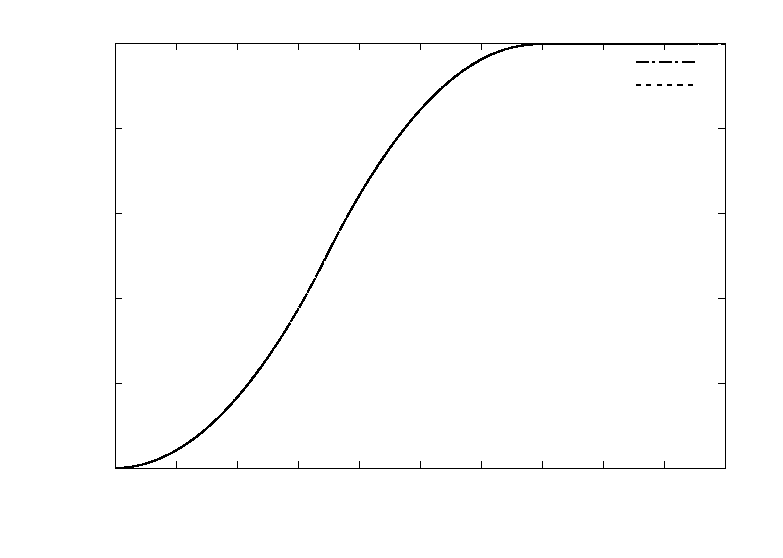
\includegraphics{accresponse}}%
    \gplfronttext
  \end{picture}%
\endgroup

    \caption{Cart position time history. Note that the displacement between the carts is negligible.}%
    \label{f:accresponse}
\end{figure}

%\begin{figure}
    %\centering
    %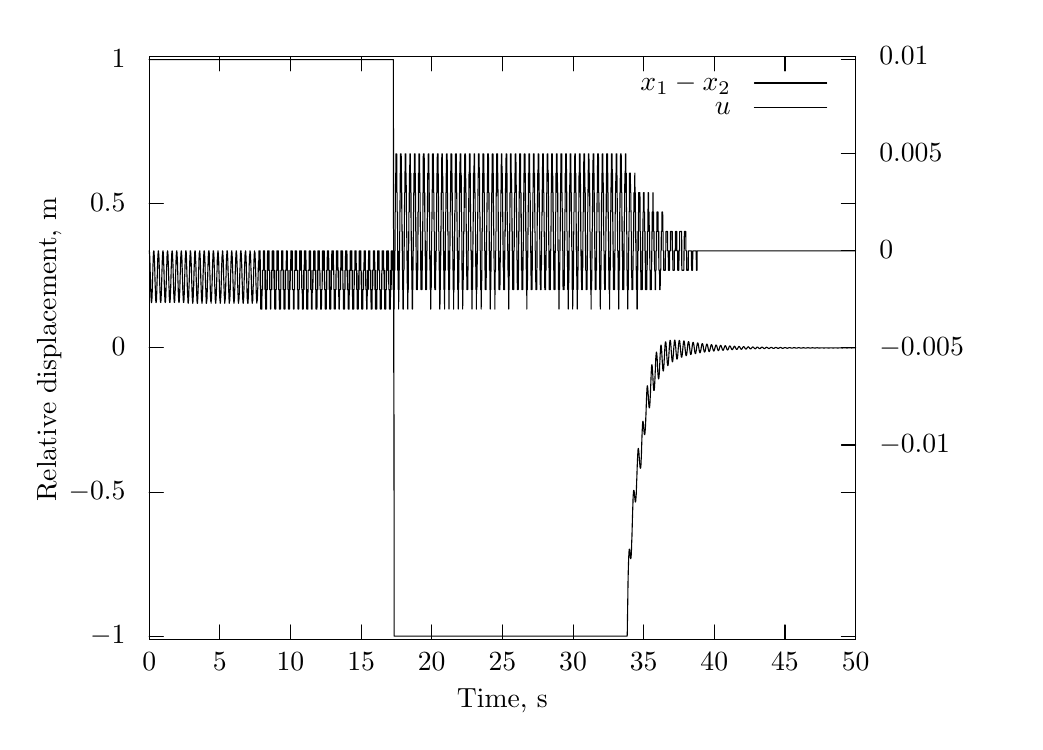
\begin{tikzpicture}[gnuplot]
%% generated with GNUPLOT 5.0p3 (Lua 5.1; terminal rev. 99, script rev. 100)
%% Tue 27 Mar 2018 11:23:02 PM EDT
\gpmonochromelines
\path (0.000,0.000) rectangle (12.500,8.750);
\gpcolor{color=gp lt color border}
\gpsetlinetype{gp lt border}
\gpsetdashtype{gp dt solid}
\gpsetlinewidth{1.00}
\draw[gp path] (1.504,1.022)--(1.684,1.022);
\draw[gp path] (10.475,1.022)--(10.295,1.022);
\node[gp node right] at (1.320,1.022) {$-1$};
\draw[gp path] (1.504,2.852)--(1.684,2.852);
\draw[gp path] (10.475,2.852)--(10.295,2.852);
\node[gp node right] at (1.320,2.852) {$-0.5$};
\draw[gp path] (1.504,4.683)--(1.684,4.683);
\draw[gp path] (10.475,4.683)--(10.295,4.683);
\node[gp node right] at (1.320,4.683) {$0$};
\draw[gp path] (1.504,6.514)--(1.684,6.514);
\draw[gp path] (10.475,6.514)--(10.295,6.514);
\node[gp node right] at (1.320,6.514) {$0.5$};
\draw[gp path] (1.504,8.344)--(1.684,8.344);
\draw[gp path] (10.475,8.344)--(10.295,8.344);
\node[gp node right] at (1.320,8.344) {$1$};
\draw[gp path] (1.504,0.985)--(1.504,1.165);
\draw[gp path] (1.504,8.381)--(1.504,8.201);
\node[gp node center] at (1.504,0.677) {$0$};
\draw[gp path] (2.401,0.985)--(2.401,1.165);
\draw[gp path] (2.401,8.381)--(2.401,8.201);
\node[gp node center] at (2.401,0.677) {$5$};
\draw[gp path] (3.298,0.985)--(3.298,1.165);
\draw[gp path] (3.298,8.381)--(3.298,8.201);
\node[gp node center] at (3.298,0.677) {$10$};
\draw[gp path] (4.195,0.985)--(4.195,1.165);
\draw[gp path] (4.195,8.381)--(4.195,8.201);
\node[gp node center] at (4.195,0.677) {$15$};
\draw[gp path] (5.092,0.985)--(5.092,1.165);
\draw[gp path] (5.092,8.381)--(5.092,8.201);
\node[gp node center] at (5.092,0.677) {$20$};
\draw[gp path] (5.990,0.985)--(5.990,1.165);
\draw[gp path] (5.990,8.381)--(5.990,8.201);
\node[gp node center] at (5.990,0.677) {$25$};
\draw[gp path] (6.887,0.985)--(6.887,1.165);
\draw[gp path] (6.887,8.381)--(6.887,8.201);
\node[gp node center] at (6.887,0.677) {$30$};
\draw[gp path] (7.784,0.985)--(7.784,1.165);
\draw[gp path] (7.784,8.381)--(7.784,8.201);
\node[gp node center] at (7.784,0.677) {$35$};
\draw[gp path] (8.681,0.985)--(8.681,1.165);
\draw[gp path] (8.681,8.381)--(8.681,8.201);
\node[gp node center] at (8.681,0.677) {$40$};
\draw[gp path] (9.578,0.985)--(9.578,1.165);
\draw[gp path] (9.578,8.381)--(9.578,8.201);
\node[gp node center] at (9.578,0.677) {$45$};
\draw[gp path] (10.475,0.985)--(10.475,1.165);
\draw[gp path] (10.475,8.381)--(10.475,8.201);
\node[gp node center] at (10.475,0.677) {$50$};
\draw[gp path] (10.475,3.450)--(10.295,3.450);
\node[gp node left] at (10.659,3.450) {$-0.01$};
\draw[gp path] (10.475,4.683)--(10.295,4.683);
\node[gp node left] at (10.659,4.683) {$-0.005$};
\draw[gp path] (10.475,5.916)--(10.295,5.916);
\node[gp node left] at (10.659,5.916) {$0$};
\draw[gp path] (10.475,7.148)--(10.295,7.148);
\node[gp node left] at (10.659,7.148) {$0.005$};
\draw[gp path] (10.475,8.381)--(10.295,8.381);
\node[gp node left] at (10.659,8.381) {$0.01$};
\draw[gp path] (1.504,8.381)--(1.504,0.985)--(10.475,0.985)--(10.475,8.381)--cycle;
\node[gp node center,rotate=-270] at (0.246,4.683) {Relative displacement, m};
\node[gp node center] at (5.989,0.215) {Time, s};
\node[gp node right] at (9.007,8.047) {$x_1-x_2$};
\draw[gp path] (9.191,8.047)--(10.107,8.047);
\draw[gp path] (1.504,5.916)--(1.505,5.915)--(1.505,5.912)--(1.506,5.907)--(1.507,5.900)%
  --(1.508,5.892)--(1.508,5.881)--(1.509,5.869)--(1.510,5.855)--(1.511,5.831)--(1.512,5.803)%
  --(1.513,5.772)--(1.514,5.739)--(1.515,5.703)--(1.516,5.665)--(1.517,5.626)--(1.519,5.587)%
  --(1.520,5.544)--(1.521,5.502)--(1.522,5.462)--(1.523,5.424)--(1.525,5.380)--(1.526,5.342)%
  --(1.528,5.310)--(1.529,5.285)--(1.531,5.271)--(1.532,5.262)--(1.533,5.258)--(1.534,5.260)%
  --(1.535,5.266)--(1.536,5.277)--(1.537,5.292)--(1.539,5.312)--(1.540,5.336)--(1.541,5.362)%
  --(1.542,5.392)--(1.543,5.425)--(1.544,5.460)--(1.545,5.497)--(1.546,5.536)--(1.547,5.575)%
  --(1.549,5.617)--(1.550,5.659)--(1.551,5.699)--(1.552,5.738)--(1.554,5.782)--(1.555,5.821)%
  --(1.556,5.854)--(1.558,5.881)--(1.559,5.897)--(1.560,5.908)--(1.561,5.914)--(1.563,5.915)%
  --(1.564,5.911)--(1.565,5.903)--(1.566,5.889)--(1.567,5.870)--(1.568,5.848)--(1.569,5.823)%
  --(1.570,5.794)--(1.572,5.763)--(1.573,5.729)--(1.574,5.692)--(1.575,5.654)--(1.576,5.616)%
  --(1.577,5.574)--(1.578,5.532)--(1.579,5.492)--(1.581,5.452)--(1.582,5.409)--(1.583,5.369)%
  --(1.585,5.335)--(1.586,5.306)--(1.587,5.287)--(1.589,5.272)--(1.590,5.263)--(1.591,5.258)%
  --(1.592,5.260)--(1.593,5.266)--(1.595,5.278)--(1.596,5.294)--(1.597,5.314)--(1.598,5.338)%
  --(1.599,5.365)--(1.600,5.395)--(1.601,5.428)--(1.602,5.463)--(1.603,5.500)--(1.604,5.538)%
  --(1.606,5.579)--(1.607,5.621)--(1.608,5.661)--(1.609,5.701)--(1.611,5.744)--(1.612,5.785)%
  --(1.613,5.821)--(1.615,5.852)--(1.616,5.875)--(1.617,5.893)--(1.618,5.906)--(1.619,5.913)%
  --(1.621,5.916)--(1.622,5.912)--(1.623,5.903)--(1.624,5.889)--(1.625,5.871)--(1.626,5.849)%
  --(1.628,5.823)--(1.629,5.795)--(1.630,5.763)--(1.631,5.729)--(1.632,5.693)--(1.633,5.656)%
  --(1.634,5.615)--(1.635,5.574)--(1.636,5.534)--(1.638,5.494)--(1.639,5.450)--(1.640,5.410)%
  --(1.642,5.372)--(1.643,5.339)--(1.644,5.314)--(1.645,5.292)--(1.647,5.272)--(1.648,5.265)%
  --(1.649,5.260)--(1.650,5.260)--(1.652,5.267)--(1.653,5.280)--(1.654,5.294)--(1.655,5.317)%
  --(1.656,5.341)--(1.657,5.368)--(1.658,5.400)--(1.660,5.432)--(1.661,5.469)--(1.662,5.504)%
  --(1.663,5.546)--(1.664,5.585)--(1.665,5.625)--(1.666,5.664)--(1.668,5.709)--(1.669,5.748)%
  --(1.670,5.787)--(1.671,5.822)--(1.673,5.854)--(1.674,5.876)--(1.675,5.893)--(1.677,5.908)%
  --(1.678,5.916)--(1.679,5.916)--(1.680,5.908)--(1.682,5.896)--(1.683,5.881)--(1.684,5.861)%
  --(1.685,5.839)--(1.686,5.812)--(1.687,5.780)--(1.688,5.748)--(1.690,5.716)--(1.691,5.679)%
  --(1.692,5.640)--(1.693,5.598)--(1.694,5.558)--(1.695,5.516)--(1.696,5.474)--(1.698,5.432)%
  --(1.699,5.395)--(1.700,5.361)--(1.702,5.329)--(1.703,5.304)--(1.704,5.285)--(1.705,5.270)%
  --(1.707,5.260)--(1.708,5.260)--(1.709,5.262)--(1.711,5.275)--(1.712,5.289)--(1.713,5.309)%
  --(1.714,5.329)--(1.715,5.359)--(1.716,5.386)--(1.717,5.418)--(1.718,5.455)--(1.720,5.492)%
  --(1.721,5.531)--(1.722,5.571)--(1.723,5.610)--(1.724,5.649)--(1.725,5.694)--(1.727,5.733)%
  --(1.728,5.773)--(1.729,5.807)--(1.730,5.842)--(1.732,5.866)--(1.733,5.889)--(1.734,5.903)%
  --(1.736,5.913)--(1.737,5.916)--(1.738,5.913)--(1.740,5.901)--(1.741,5.886)--(1.742,5.869)%
  --(1.743,5.844)--(1.744,5.820)--(1.745,5.790)--(1.746,5.755)--(1.747,5.723)--(1.749,5.686)%
  --(1.750,5.649)--(1.751,5.608)--(1.752,5.568)--(1.753,5.526)--(1.754,5.484)--(1.756,5.442)%
  --(1.757,5.403)--(1.758,5.366)--(1.759,5.334)--(1.761,5.307)--(1.762,5.285)--(1.763,5.270)%
  --(1.765,5.262)--(1.766,5.260)--(1.767,5.262)--(1.769,5.272)--(1.770,5.287)--(1.771,5.307)%
  --(1.772,5.326)--(1.773,5.354)--(1.774,5.383)--(1.775,5.418)--(1.777,5.450)--(1.778,5.487)%
  --(1.779,5.526)--(1.780,5.563)--(1.781,5.605)--(1.782,5.644)--(1.783,5.686)--(1.785,5.728)%
  --(1.786,5.768)--(1.787,5.805)--(1.789,5.837)--(1.790,5.866)--(1.791,5.886)--(1.793,5.903)%
  --(1.794,5.913)--(1.795,5.916)--(1.797,5.911)--(1.798,5.901)--(1.799,5.886)--(1.800,5.869)%
  --(1.801,5.847)--(1.802,5.820)--(1.803,5.792)--(1.805,5.760)--(1.806,5.726)--(1.807,5.689)%
  --(1.808,5.649)--(1.809,5.610)--(1.810,5.568)--(1.811,5.531)--(1.813,5.487)--(1.814,5.445)%
  --(1.815,5.405)--(1.816,5.371)--(1.818,5.339)--(1.819,5.309)--(1.820,5.287)--(1.822,5.272)%
  --(1.823,5.262)--(1.824,5.260)--(1.826,5.262)--(1.827,5.272)--(1.828,5.287)--(1.829,5.304)%
  --(1.830,5.329)--(1.831,5.354)--(1.833,5.383)--(1.834,5.413)--(1.835,5.450)--(1.836,5.487)%
  --(1.837,5.524)--(1.838,5.563)--(1.839,5.603)--(1.840,5.644)--(1.842,5.686)--(1.843,5.728)%
  --(1.844,5.768)--(1.845,5.802)--(1.847,5.837)--(1.848,5.864)--(1.849,5.886)--(1.851,5.903)%
  --(1.852,5.911)--(1.853,5.916)--(1.855,5.911)--(1.856,5.901)--(1.857,5.889)--(1.858,5.869)%
  --(1.859,5.847)--(1.861,5.820)--(1.862,5.792)--(1.863,5.760)--(1.864,5.726)--(1.865,5.689)%
  --(1.866,5.649)--(1.867,5.612)--(1.868,5.571)--(1.869,5.531)--(1.871,5.487)--(1.872,5.447)%
  --(1.873,5.405)--(1.874,5.371)--(1.876,5.336)--(1.877,5.309)--(1.878,5.287)--(1.880,5.270)%
  --(1.881,5.260)--(1.882,5.260)--(1.884,5.262)--(1.885,5.272)--(1.886,5.287)--(1.887,5.304)%
  --(1.889,5.329)--(1.890,5.354)--(1.891,5.383)--(1.892,5.415)--(1.893,5.447)--(1.894,5.484)%
  --(1.895,5.521)--(1.896,5.563)--(1.897,5.605)--(1.899,5.644)--(1.900,5.686)--(1.901,5.728)%
  --(1.902,5.765)--(1.904,5.802)--(1.905,5.837)--(1.906,5.864)--(1.908,5.886)--(1.909,5.903)%
  --(1.910,5.911)--(1.912,5.916)--(1.913,5.911)--(1.914,5.903)--(1.915,5.886)--(1.916,5.869)%
  --(1.918,5.847)--(1.919,5.820)--(1.920,5.790)--(1.921,5.758)--(1.922,5.726)--(1.923,5.691)%
  --(1.924,5.649)--(1.925,5.612)--(1.927,5.568)--(1.928,5.531)--(1.929,5.487)--(1.930,5.445)%
  --(1.931,5.408)--(1.933,5.371)--(1.934,5.339)--(1.935,5.309)--(1.937,5.287)--(1.938,5.272)%
  --(1.939,5.262)--(1.941,5.260)--(1.942,5.262)--(1.943,5.267)--(1.944,5.275)--(1.946,5.299)%
  --(1.947,5.324)--(1.948,5.349)--(1.949,5.373)--(1.950,5.423)--(1.951,5.447)--(1.952,5.497)%
  --(1.953,5.521)--(1.954,5.571)--(1.956,5.620)--(1.957,5.644)--(1.958,5.694)--(1.959,5.743)%
  --(1.961,5.768)--(1.962,5.817)--(1.963,5.842)--(1.964,5.866)--(1.966,5.866)--(1.967,5.916)%
  --(1.968,5.916)--(1.970,5.916)--(1.971,5.891)--(1.972,5.916)--(1.974,5.891)--(1.975,5.866)%
  --(1.976,5.842)--(1.977,5.817)--(1.978,5.792)--(1.979,5.743)--(1.980,5.718)--(1.981,5.694)%
  --(1.982,5.644)--(1.984,5.595)--(1.985,5.571)--(1.986,5.521)--(1.987,5.497)--(1.988,5.447)%
  --(1.990,5.398)--(1.991,5.373)--(1.992,5.324)--(1.994,5.324)--(1.995,5.299)--(1.996,5.275)%
  --(1.998,5.250)--(1.999,5.250)--(2.000,5.275)--(2.002,5.275)--(2.003,5.299)--(2.004,5.299)%
  --(2.005,5.324)--(2.006,5.349)--(2.007,5.398)--(2.008,5.423)--(2.009,5.447)--(2.010,5.472)%
  --(2.012,5.521)--(2.013,5.571)--(2.014,5.595)--(2.015,5.644)--(2.016,5.669)--(2.018,5.718)%
  --(2.019,5.768)--(2.020,5.817)--(2.021,5.842)--(2.023,5.866)--(2.024,5.891)--(2.025,5.916)%
  --(2.027,5.916)--(2.028,5.916)--(2.029,5.916)--(2.031,5.891)--(2.032,5.891)--(2.033,5.866)%
  --(2.034,5.842)--(2.035,5.817)--(2.036,5.792)--(2.037,5.768)--(2.038,5.718)--(2.040,5.694)%
  --(2.041,5.644)--(2.042,5.620)--(2.043,5.571)--(2.044,5.521)--(2.045,5.497)--(2.047,5.447)%
  --(2.048,5.398)--(2.049,5.373)--(2.050,5.349)--(2.052,5.299)--(2.053,5.299)--(2.054,5.275)%
  --(2.056,5.275)--(2.057,5.250)--(2.058,5.250)--(2.060,5.275)--(2.061,5.275)--(2.062,5.324)%
  --(2.063,5.324)--(2.064,5.349)--(2.065,5.373)--(2.066,5.423)--(2.068,5.472)--(2.069,5.472)%
  --(2.070,5.521)--(2.071,5.571)--(2.072,5.595)--(2.073,5.644)--(2.074,5.694)--(2.076,5.718)%
  --(2.077,5.768)--(2.078,5.817)--(2.080,5.842)--(2.081,5.866)--(2.082,5.891)--(2.084,5.916)%
  --(2.085,5.916)--(2.086,5.916)--(2.088,5.916)--(2.089,5.891)--(2.090,5.891)--(2.091,5.866)%
  --(2.092,5.842)--(2.093,5.817)--(2.094,5.792)--(2.096,5.743)--(2.097,5.718)--(2.098,5.694)%
  --(2.099,5.644)--(2.100,5.595)--(2.101,5.571)--(2.102,5.521)--(2.104,5.472)--(2.105,5.447)%
  --(2.106,5.398)--(2.107,5.373)--(2.109,5.324)--(2.110,5.299)--(2.111,5.275)--(2.113,5.275)%
  --(2.114,5.250)--(2.115,5.275)--(2.117,5.250)--(2.118,5.275)--(2.119,5.299)--(2.120,5.299)%
  --(2.121,5.324)--(2.122,5.349)--(2.124,5.398)--(2.125,5.423)--(2.126,5.447)--(2.127,5.497)%
  --(2.128,5.521)--(2.129,5.546)--(2.130,5.595)--(2.131,5.644)--(2.133,5.694)--(2.134,5.718)%
  --(2.135,5.768)--(2.136,5.817)--(2.138,5.842)--(2.139,5.866)--(2.140,5.891)--(2.142,5.891)%
  --(2.143,5.891)--(2.144,5.916)--(2.146,5.916)--(2.147,5.916)--(2.148,5.891)--(2.149,5.866)%
  --(2.150,5.842)--(2.152,5.817)--(2.153,5.792)--(2.154,5.768)--(2.155,5.718)--(2.156,5.669)%
  --(2.157,5.644)--(2.158,5.620)--(2.159,5.571)--(2.161,5.521)--(2.162,5.497)--(2.163,5.447)%
  --(2.164,5.423)--(2.166,5.373)--(2.167,5.349)--(2.168,5.299)--(2.170,5.299)--(2.171,5.275)%
  --(2.172,5.275)--(2.174,5.250)--(2.175,5.275)--(2.176,5.275)--(2.177,5.275)--(2.178,5.299)%
  --(2.180,5.324)--(2.181,5.349)--(2.182,5.373)--(2.183,5.423)--(2.184,5.447)--(2.185,5.497)%
  --(2.186,5.521)--(2.187,5.571)--(2.188,5.620)--(2.190,5.644)--(2.191,5.694)--(2.192,5.743)%
  --(2.193,5.768)--(2.195,5.817)--(2.196,5.842)--(2.197,5.866)--(2.199,5.891)--(2.200,5.916)%
  --(2.201,5.891)--(2.203,5.916)--(2.204,5.916)--(2.205,5.916)--(2.206,5.891)--(2.208,5.866)%
  --(2.209,5.842)--(2.210,5.842)--(2.211,5.792)--(2.212,5.768)--(2.213,5.718)--(2.214,5.694)%
  --(2.215,5.644)--(2.216,5.620)--(2.218,5.571)--(2.219,5.521)--(2.220,5.497)--(2.221,5.447)%
  --(2.223,5.423)--(2.224,5.373)--(2.225,5.349)--(2.226,5.324)--(2.228,5.299)--(2.229,5.250)%
  --(2.230,5.250)--(2.232,5.275)--(2.233,5.250)--(2.234,5.275)--(2.236,5.299)--(2.237,5.299)%
  --(2.238,5.324)--(2.239,5.349)--(2.240,5.373)--(2.241,5.423)--(2.242,5.447)--(2.243,5.497)%
  --(2.244,5.521)--(2.246,5.571)--(2.247,5.595)--(2.248,5.644)--(2.249,5.694)--(2.250,5.718)%
  --(2.252,5.768)--(2.253,5.792)--(2.254,5.842)--(2.256,5.866)--(2.257,5.866)--(2.258,5.916)%
  --(2.260,5.916)--(2.261,5.916)--(2.262,5.916)--(2.264,5.916)--(2.265,5.891)--(2.266,5.891)%
  --(2.267,5.866)--(2.268,5.842)--(2.269,5.768)--(2.270,5.743)--(2.271,5.718)--(2.272,5.669)%
  --(2.274,5.669)--(2.275,5.620)--(2.276,5.571)--(2.277,5.521)--(2.278,5.497)--(2.279,5.447)%
  --(2.281,5.398)--(2.282,5.373)--(2.283,5.324)--(2.285,5.299)--(2.286,5.275)--(2.287,5.275)%
  --(2.289,5.275)--(2.290,5.250)--(2.291,5.275)--(2.293,5.275)--(2.294,5.299)--(2.295,5.299)%
  --(2.296,5.324)--(2.297,5.373)--(2.298,5.373)--(2.299,5.398)--(2.300,5.447)--(2.302,5.497)%
  --(2.303,5.521)--(2.304,5.546)--(2.305,5.620)--(2.306,5.644)--(2.307,5.694)--(2.309,5.743)%
  --(2.310,5.768)--(2.311,5.792)--(2.312,5.817)--(2.314,5.866)--(2.315,5.891)--(2.316,5.916)%
  --(2.318,5.916)--(2.319,5.916)--(2.320,5.916)--(2.322,5.916)--(2.323,5.891)--(2.324,5.866)%
  --(2.325,5.842)--(2.326,5.842)--(2.327,5.792)--(2.328,5.768)--(2.330,5.718)--(2.331,5.694)%
  --(2.332,5.644)--(2.333,5.620)--(2.334,5.571)--(2.335,5.521)--(2.336,5.472)--(2.338,5.447)%
  --(2.339,5.423)--(2.340,5.373)--(2.342,5.324)--(2.343,5.299)--(2.344,5.275)--(2.346,5.275)%
  --(2.347,5.250)--(2.348,5.250)--(2.350,5.250)--(2.351,5.275)--(2.352,5.299)--(2.353,5.299)%
  --(2.354,5.324)--(2.355,5.349)--(2.356,5.373)--(2.358,5.423)--(2.359,5.447)--(2.360,5.472)%
  --(2.361,5.521)--(2.362,5.571)--(2.363,5.595)--(2.364,5.644)--(2.366,5.669)--(2.367,5.718)%
  --(2.368,5.768)--(2.369,5.817)--(2.371,5.842)--(2.372,5.842)--(2.373,5.891)--(2.375,5.891)%
  --(2.376,5.916)--(2.377,5.916)--(2.379,5.916)--(2.380,5.891)--(2.381,5.891)--(2.382,5.866)%
  --(2.383,5.842)--(2.384,5.842)--(2.386,5.792)--(2.387,5.768)--(2.388,5.718)--(2.389,5.694)%
  --(2.390,5.644)--(2.391,5.620)--(2.392,5.571)--(2.393,5.546)--(2.395,5.497)--(2.396,5.447)%
  --(2.397,5.398)--(2.398,5.373)--(2.400,5.324)--(2.401,5.299)--(2.402,5.299)--(2.404,5.275)%
  --(2.405,5.250)--(2.406,5.275)--(2.408,5.250)--(2.409,5.275)--(2.410,5.275)--(2.411,5.299)%
  --(2.412,5.324)--(2.414,5.349)--(2.415,5.373)--(2.416,5.398)--(2.417,5.447)--(2.418,5.472)%
  --(2.419,5.521)--(2.420,5.546)--(2.421,5.595)--(2.422,5.644)--(2.424,5.694)--(2.425,5.718)%
  --(2.426,5.768)--(2.428,5.792)--(2.429,5.842)--(2.430,5.866)--(2.432,5.866)--(2.433,5.891)%
  --(2.434,5.916)--(2.436,5.916)--(2.437,5.916)--(2.438,5.891)--(2.439,5.866)--(2.440,5.866)%
  --(2.442,5.842)--(2.443,5.817)--(2.444,5.792)--(2.445,5.768)--(2.446,5.718)--(2.447,5.694)%
  --(2.448,5.644)--(2.449,5.620)--(2.450,5.571)--(2.452,5.521)--(2.453,5.497)--(2.454,5.447)%
  --(2.455,5.423)--(2.457,5.373)--(2.458,5.324)--(2.459,5.299)--(2.461,5.299)--(2.462,5.275)%
  --(2.463,5.250)--(2.465,5.275)--(2.466,5.275)--(2.467,5.275)--(2.468,5.275)--(2.470,5.324)%
  --(2.471,5.349)--(2.472,5.349)--(2.473,5.373)--(2.474,5.423)--(2.475,5.447)--(2.476,5.497)%
  --(2.477,5.521)--(2.478,5.571)--(2.480,5.595)--(2.481,5.644)--(2.482,5.694)--(2.483,5.743)%
  --(2.484,5.768)--(2.486,5.817)--(2.487,5.842)--(2.488,5.842)--(2.490,5.891)--(2.491,5.916)%
  --(2.492,5.916)--(2.494,5.916)--(2.495,5.916)--(2.496,5.916)--(2.498,5.891)--(2.499,5.866)%
  --(2.500,5.842)--(2.501,5.817)--(2.502,5.792)--(2.503,5.768)--(2.504,5.718)--(2.505,5.669)%
  --(2.506,5.644)--(2.508,5.620)--(2.509,5.571)--(2.510,5.546)--(2.511,5.497)--(2.512,5.447)%
  --(2.514,5.423)--(2.515,5.373)--(2.516,5.324)--(2.518,5.299)--(2.519,5.299)--(2.520,5.250)%
  --(2.522,5.250)--(2.523,5.275)--(2.524,5.275)--(2.526,5.275)--(2.527,5.299)--(2.528,5.299)%
  --(2.529,5.324)--(2.530,5.349)--(2.531,5.373)--(2.532,5.398)--(2.533,5.447)--(2.534,5.497)%
  --(2.536,5.521)--(2.537,5.571)--(2.538,5.620)--(2.539,5.644)--(2.540,5.669)--(2.541,5.743)%
  --(2.543,5.768)--(2.544,5.817)--(2.545,5.817)--(2.547,5.866)--(2.548,5.866)--(2.549,5.891)%
  --(2.551,5.916)--(2.552,5.916)--(2.553,5.916)--(2.555,5.891)--(2.556,5.891)--(2.557,5.866)%
  --(2.558,5.842)--(2.559,5.817)--(2.560,5.792)--(2.561,5.743)--(2.562,5.718)--(2.563,5.669)%
  --(2.565,5.644)--(2.566,5.620)--(2.567,5.571)--(2.568,5.521)--(2.569,5.497)--(2.571,5.447)%
  --(2.572,5.398)--(2.573,5.349)--(2.574,5.324)--(2.576,5.299)--(2.577,5.299)--(2.578,5.275)%
  --(2.580,5.250)--(2.581,5.275)--(2.582,5.275)--(2.584,5.275)--(2.585,5.299)--(2.586,5.299)%
  --(2.587,5.324)--(2.588,5.349)--(2.589,5.398)--(2.590,5.423)--(2.592,5.447)--(2.593,5.497)%
  --(2.594,5.521)--(2.595,5.546)--(2.596,5.620)--(2.597,5.644)--(2.598,5.694)--(2.600,5.718)%
  --(2.601,5.768)--(2.602,5.792)--(2.604,5.842)--(2.605,5.866)--(2.606,5.891)--(2.608,5.891)%
  --(2.609,5.916)--(2.610,5.916)--(2.611,5.916)--(2.613,5.891)--(2.614,5.891)--(2.615,5.866)%
  --(2.616,5.842)--(2.617,5.817)--(2.618,5.792)--(2.620,5.743)--(2.621,5.718)--(2.622,5.669)%
  --(2.623,5.644)--(2.624,5.595)--(2.625,5.571)--(2.626,5.521)--(2.627,5.497)--(2.629,5.447)%
  --(2.630,5.398)--(2.631,5.373)--(2.633,5.349)--(2.634,5.299)--(2.635,5.275)--(2.637,5.275)%
  --(2.638,5.250)--(2.639,5.275)--(2.641,5.275)--(2.642,5.275)--(2.643,5.299)--(2.644,5.299)%
  --(2.645,5.324)--(2.646,5.349)--(2.648,5.373)--(2.649,5.423)--(2.650,5.447)--(2.651,5.472)%
  --(2.652,5.521)--(2.653,5.546)--(2.654,5.620)--(2.655,5.644)--(2.657,5.669)--(2.658,5.718)%
  --(2.659,5.768)--(2.660,5.792)--(2.662,5.842)--(2.663,5.866)--(2.664,5.891)--(2.666,5.916)%
  --(2.667,5.891)--(2.668,5.916)--(2.670,5.916)--(2.671,5.891)--(2.672,5.891)--(2.673,5.866)%
  --(2.674,5.842)--(2.676,5.817)--(2.677,5.792)--(2.678,5.768)--(2.679,5.718)--(2.680,5.694)%
  --(2.681,5.644)--(2.682,5.620)--(2.683,5.571)--(2.684,5.546)--(2.686,5.497)--(2.687,5.447)%
  --(2.688,5.398)--(2.689,5.373)--(2.691,5.349)--(2.692,5.324)--(2.693,5.275)--(2.695,5.275)%
  --(2.696,5.250)--(2.697,5.275)--(2.699,5.250)--(2.700,5.275)--(2.701,5.275)--(2.702,5.299)%
  --(2.704,5.324)--(2.705,5.349)--(2.706,5.373)--(2.707,5.423)--(2.708,5.447)--(2.709,5.497)%
  --(2.710,5.546)--(2.711,5.546)--(2.712,5.595)--(2.714,5.644)--(2.715,5.694)--(2.716,5.743)%
  --(2.717,5.768)--(2.719,5.792)--(2.720,5.842)--(2.721,5.866)--(2.723,5.866)--(2.724,5.891)%
  --(2.725,5.916)--(2.727,5.916)--(2.728,5.916)--(2.729,5.916)--(2.730,5.891)--(2.732,5.866)%
  --(2.733,5.842)--(2.734,5.817)--(2.735,5.792)--(2.736,5.768)--(2.737,5.718)--(2.738,5.694)%
  --(2.739,5.644)--(2.740,5.595)--(2.742,5.571)--(2.743,5.521)--(2.744,5.472)--(2.745,5.447)%
  --(2.746,5.398)--(2.748,5.349)--(2.749,5.324)--(2.750,5.299)--(2.752,5.299)--(2.753,5.275)%
  --(2.754,5.275)--(2.756,5.250)--(2.757,5.250)--(2.758,5.250)--(2.759,5.299)--(2.761,5.299)%
  --(2.762,5.324)--(2.763,5.349)--(2.764,5.373)--(2.765,5.423)--(2.766,5.447)--(2.767,5.472)%
  --(2.768,5.521)--(2.770,5.546)--(2.771,5.595)--(2.772,5.644)--(2.773,5.694)--(2.774,5.743)%
  --(2.776,5.768)--(2.777,5.817)--(2.778,5.842)--(2.779,5.866)--(2.781,5.866)--(2.782,5.891)%
  --(2.783,5.916)--(2.785,5.916)--(2.786,5.916)--(2.787,5.891)--(2.789,5.891)--(2.790,5.866)%
  --(2.791,5.866)--(2.792,5.842)--(2.793,5.792)--(2.794,5.768)--(2.795,5.718)--(2.796,5.694)%
  --(2.797,5.669)--(2.799,5.620)--(2.800,5.571)--(2.801,5.521)--(2.802,5.472)--(2.803,5.447)%
  --(2.805,5.398)--(2.806,5.373)--(2.807,5.349)--(2.809,5.299)--(2.810,5.275)--(2.811,5.275)%
  --(2.813,5.250)--(2.814,5.250)--(2.815,5.275)--(2.817,5.275)--(2.818,5.275)--(2.819,5.299)%
  --(2.820,5.324)--(2.821,5.349)--(2.822,5.398)--(2.823,5.423)--(2.824,5.447)--(2.825,5.472)%
  --(2.827,5.521)--(2.828,5.571)--(2.829,5.595)--(2.830,5.644)--(2.831,5.694)--(2.833,5.718)%
  --(2.834,5.768)--(2.835,5.792)--(2.836,5.842)--(2.838,5.866)--(2.839,5.891)--(2.840,5.891)%
  --(2.842,5.916)--(2.843,5.916)--(2.844,5.891)--(2.846,5.891)--(2.847,5.891)--(2.848,5.866)%
  --(2.849,5.842)--(2.850,5.817)--(2.851,5.792)--(2.852,5.768)--(2.853,5.718)--(2.855,5.669)%
  --(2.856,5.644)--(2.857,5.620)--(2.858,5.571)--(2.859,5.521)--(2.860,5.497)--(2.862,5.447)%
  --(2.863,5.398)--(2.864,5.373)--(2.865,5.324)--(2.867,5.299)--(2.868,5.299)--(2.869,5.275)%
  --(2.871,5.250)--(2.872,5.275)--(2.873,5.275)--(2.875,5.275)--(2.876,5.299)--(2.877,5.324)%
  --(2.878,5.324)--(2.879,5.349)--(2.880,5.373)--(2.881,5.423)--(2.883,5.447)--(2.884,5.472)%
  --(2.885,5.546)--(2.886,5.571)--(2.887,5.620)--(2.888,5.644)--(2.889,5.694)--(2.891,5.718)%
  --(2.892,5.768)--(2.893,5.792)--(2.895,5.669)--(2.896,5.669)--(2.897,5.916)--(2.899,5.916)%
  --(2.900,5.916)--(2.901,5.916)--(2.903,5.916)--(2.904,5.916)--(2.905,5.916)--(2.906,5.916)%
  --(2.907,5.916)--(2.908,5.916)--(2.909,5.916)--(2.911,5.916)--(2.912,5.916)--(2.913,5.916)%
  --(2.914,5.669)--(2.915,5.423)--(2.916,5.669)--(2.917,5.423)--(2.919,5.669)--(2.920,5.423)%
  --(2.921,5.176)--(2.922,5.423)--(2.924,5.176)--(2.925,5.423)--(2.926,5.423)--(2.928,5.176)%
  --(2.929,5.423)--(2.930,5.176)--(2.932,5.176)--(2.933,5.176)--(2.934,5.423)--(2.935,5.176)%
  --(2.936,5.423)--(2.938,5.423)--(2.939,5.423)--(2.940,5.423)--(2.941,5.423)--(2.942,5.423)%
  --(2.943,5.423)--(2.944,5.423)--(2.945,5.669)--(2.946,5.669)--(2.948,5.669)--(2.949,5.669)%
  --(2.950,5.669)--(2.951,5.669)--(2.953,5.669)--(2.954,5.669)--(2.955,5.916)--(2.957,5.916)%
  --(2.958,5.916)--(2.959,5.916)--(2.961,5.916)--(2.962,5.916)--(2.963,5.916)--(2.964,5.916)%
  --(2.966,5.916)--(2.967,5.916)--(2.968,5.669)--(2.969,5.916)--(2.970,5.669)--(2.971,5.669)%
  --(2.972,5.669)--(2.973,5.669)--(2.974,5.423)--(2.976,5.423)--(2.977,5.669)--(2.978,5.423)%
  --(2.979,5.423)--(2.981,5.423)--(2.982,5.176)--(2.983,5.423)--(2.985,5.176)--(2.986,5.423)%
  --(2.987,5.176)--(2.989,5.423)--(2.990,5.176)--(2.991,5.423)--(2.992,5.176)--(2.994,5.176)%
  --(2.995,5.423)--(2.996,5.423)--(2.997,5.423)--(2.998,5.423)--(2.999,5.423)--(3.000,5.423)%
  --(3.001,5.669)--(3.002,5.669)--(3.004,5.423)--(3.005,5.669)--(3.006,5.669)--(3.007,5.916)%
  --(3.008,5.669)--(3.010,5.669)--(3.011,5.916)--(3.012,5.916)--(3.014,5.916)--(3.015,5.916)%
  --(3.016,5.916)--(3.018,5.916)--(3.019,5.669)--(3.020,5.916)--(3.022,5.916)--(3.023,5.916)%
  --(3.024,5.916)--(3.025,5.916)--(3.026,5.916)--(3.027,5.669)--(3.028,5.669)--(3.029,5.669)%
  --(3.030,5.669)--(3.032,5.669)--(3.033,5.669)--(3.034,5.669)--(3.035,5.423)--(3.036,5.423)%
  --(3.038,5.423)--(3.039,5.423)--(3.040,5.423)--(3.042,5.423)--(3.043,5.176)--(3.044,5.176)%
  --(3.046,5.423)--(3.047,5.176)--(3.048,5.176)--(3.050,5.423)--(3.051,5.423)--(3.052,5.423)%
  --(3.053,5.423)--(3.054,5.423)--(3.055,5.423)--(3.056,5.423)--(3.057,5.423)--(3.058,5.423)%
  --(3.060,5.669)--(3.061,5.423)--(3.062,5.669)--(3.063,5.669)--(3.064,5.669)--(3.065,5.669)%
  --(3.067,5.916)--(3.068,5.669)--(3.069,5.916)--(3.071,5.916)--(3.072,5.669)--(3.073,5.916)%
  --(3.075,5.916)--(3.076,5.916)--(3.077,5.916)--(3.079,5.916)--(3.080,5.916)--(3.081,5.669)%
  --(3.082,5.916)--(3.083,5.916)--(3.084,5.916)--(3.085,5.916)--(3.086,5.669)--(3.088,5.669)%
  --(3.089,5.669)--(3.090,5.423)--(3.091,5.669)--(3.092,5.669)--(3.093,5.423)--(3.095,5.423)%
  --(3.096,5.423)--(3.097,5.423)--(3.099,5.176)--(3.100,5.176)--(3.101,5.176)--(3.102,5.176)%
  --(3.104,5.176)--(3.105,5.176)--(3.106,5.423)--(3.108,5.423)--(3.109,5.176)--(3.110,5.423)%
  --(3.111,5.423)--(3.112,5.176)--(3.113,5.423)--(3.114,5.423)--(3.116,5.423)--(3.117,5.423)%
  --(3.118,5.669)--(3.119,5.669)--(3.120,5.669)--(3.121,5.669)--(3.122,5.669)--(3.124,5.669)%
  --(3.125,5.669)--(3.126,5.916)--(3.128,5.669)--(3.129,5.916)--(3.130,5.916)--(3.132,5.916)%
  --(3.133,5.916)--(3.134,5.916)--(3.136,5.916)--(3.137,5.916)--(3.138,5.669)--(3.139,5.669)%
  --(3.140,5.669)--(3.141,5.669)--(3.143,5.916)--(3.144,5.669)--(3.145,5.669)--(3.146,5.669)%
  --(3.147,5.423)--(3.148,5.669)--(3.149,5.669)--(3.150,5.423)--(3.152,5.423)--(3.153,5.423)%
  --(3.154,5.423)--(3.155,5.423)--(3.157,5.176)--(3.158,5.423)--(3.159,5.423)--(3.161,5.176)%
  --(3.162,5.176)--(3.163,5.176)--(3.165,5.176)--(3.166,5.176)--(3.167,5.176)--(3.168,5.423)%
  --(3.169,5.423)--(3.171,5.176)--(3.172,5.423)--(3.173,5.423)--(3.174,5.423)--(3.175,5.423)%
  --(3.176,5.423)--(3.177,5.669)--(3.178,5.669)--(3.179,5.669)--(3.181,5.669)--(3.182,5.669)%
  --(3.183,5.669)--(3.185,5.669)--(3.186,5.916)--(3.187,5.916)--(3.189,5.916)--(3.190,5.916)%
  --(3.191,5.916)--(3.193,5.916)--(3.194,5.916)--(3.195,5.916)--(3.196,5.916)--(3.197,5.916)%
  --(3.199,5.916)--(3.200,5.916)--(3.201,5.916)--(3.202,5.669)--(3.203,5.669)--(3.204,5.669)%
  --(3.205,5.669)--(3.206,5.423)--(3.208,5.423)--(3.209,5.423)--(3.210,5.669)--(3.211,5.423)%
  --(3.212,5.423)--(3.214,5.423)--(3.215,5.176)--(3.216,5.423)--(3.218,5.176)--(3.219,5.423)%
  --(3.220,5.176)--(3.222,5.176)--(3.223,5.423)--(3.224,5.176)--(3.225,5.176)--(3.227,5.176)%
  --(3.228,5.176)--(3.229,5.176)--(3.230,5.423)--(3.231,5.423)--(3.232,5.423)--(3.233,5.423)%
  --(3.234,5.669)--(3.235,5.423)--(3.237,5.669)--(3.238,5.669)--(3.239,5.669)--(3.240,5.669)%
  --(3.242,5.669)--(3.243,5.669)--(3.244,5.669)--(3.246,5.916)--(3.247,5.916)--(3.248,5.916)%
  --(3.250,5.916)--(3.251,5.916)--(3.252,5.916)--(3.253,5.916)--(3.255,5.916)--(3.256,5.916)%
  --(3.257,5.916)--(3.258,5.669)--(3.259,5.669)--(3.260,5.669)--(3.261,5.669)--(3.262,5.669)%
  --(3.263,5.669)--(3.265,5.669)--(3.266,5.669)--(3.267,5.423)--(3.268,5.423)--(3.269,5.423)%
  --(3.271,5.423)--(3.272,5.423)--(3.273,5.176)--(3.275,5.423)--(3.276,5.423)--(3.277,5.176)%
  --(3.279,5.423)--(3.280,5.176)--(3.281,5.176)--(3.283,5.423)--(3.284,5.176)--(3.285,5.176)%
  --(3.286,5.423)--(3.287,5.423)--(3.288,5.423)--(3.289,5.423)--(3.290,5.669)--(3.291,5.423)%
  --(3.293,5.423)--(3.294,5.423)--(3.295,5.669)--(3.296,5.669)--(3.297,5.669)--(3.299,5.669)%
  --(3.300,5.669)--(3.301,5.669)--(3.303,5.916)--(3.304,5.916)--(3.305,5.916)--(3.306,5.916)%
  --(3.308,5.916)--(3.309,5.916)--(3.310,5.916)--(3.312,5.669)--(3.313,5.916)--(3.314,5.916)%
  --(3.315,5.916)--(3.316,5.916)--(3.317,5.916)--(3.318,5.669)--(3.320,5.916)--(3.321,5.669)%
  --(3.322,5.669)--(3.323,5.669)--(3.324,5.423)--(3.325,5.669)--(3.326,5.423)--(3.328,5.423)%
  --(3.329,5.423)--(3.330,5.423)--(3.332,5.423)--(3.333,5.423)--(3.334,5.423)--(3.336,5.423)%
  --(3.337,5.176)--(3.338,5.176)--(3.340,5.176)--(3.341,5.423)--(3.342,5.423)--(3.343,5.176)%
  --(3.344,5.423)--(3.345,5.423)--(3.346,5.423)--(3.348,5.423)--(3.349,5.423)--(3.350,5.423)%
  --(3.351,5.669)--(3.352,5.669)--(3.353,5.669)--(3.354,5.669)--(3.356,5.669)--(3.357,5.669)%
  --(3.358,5.916)--(3.359,5.669)--(3.361,5.916)--(3.362,5.669)--(3.363,5.916)--(3.365,5.669)%
  --(3.366,5.916)--(3.367,5.916)--(3.369,5.916)--(3.370,5.916)--(3.371,5.916)--(3.372,5.916)%
  --(3.373,5.669)--(3.374,5.916)--(3.376,5.669)--(3.377,5.669)--(3.378,5.669)--(3.379,5.669)%
  --(3.380,5.669)--(3.381,5.669)--(3.382,5.669)--(3.383,5.669)--(3.385,5.669)--(3.386,5.423)%
  --(3.387,5.423)--(3.389,5.423)--(3.390,5.423)--(3.391,5.423)--(3.393,5.423)--(3.394,5.176)%
  --(3.395,5.176)--(3.397,5.176)--(3.398,5.176)--(3.399,5.176)--(3.400,5.176)--(3.401,5.176)%
  --(3.402,5.176)--(3.404,5.176)--(3.405,5.423)--(3.406,5.423)--(3.407,5.423)--(3.408,5.423)%
  --(3.409,5.669)--(3.410,5.423)--(3.411,5.669)--(3.412,5.669)--(3.414,5.669)--(3.415,5.916)%
  --(3.416,5.669)--(3.418,5.669)--(3.419,5.916)--(3.420,5.916)--(3.422,5.669)--(3.423,5.916)%
  --(3.424,5.916)--(3.426,5.916)--(3.427,5.916)--(3.428,5.916)--(3.429,5.916)--(3.431,5.916)%
  --(3.432,5.916)--(3.433,5.916)--(3.434,5.916)--(3.435,5.916)--(3.436,5.669)--(3.437,5.669)%
  --(3.438,5.669)--(3.439,5.669)--(3.440,5.669)--(3.442,5.423)--(3.443,5.423)--(3.444,5.423)%
  --(3.446,5.423)--(3.447,5.423)--(3.448,5.423)--(3.449,5.176)--(3.451,5.423)--(3.452,5.176)%
  --(3.453,5.176)--(3.455,5.423)--(3.456,5.423)--(3.457,5.176)--(3.459,5.423)--(3.460,5.423)%
  --(3.461,5.176)--(3.462,5.423)--(3.463,5.423)--(3.464,5.423)--(3.465,5.423)--(3.466,5.423)%
  --(3.467,5.669)--(3.468,5.669)--(3.470,5.423)--(3.471,5.669)--(3.472,5.669)--(3.473,5.669)%
  --(3.475,5.916)--(3.476,5.916)--(3.477,5.916)--(3.479,5.916)--(3.480,5.916)--(3.481,5.916)%
  --(3.483,5.916)--(3.484,5.916)--(3.485,5.916)--(3.487,5.916)--(3.488,5.916)--(3.489,5.669)%
  --(3.490,5.669)--(3.491,5.669)--(3.492,5.916)--(3.493,5.669)--(3.494,5.916)--(3.495,5.669)%
  --(3.496,5.669)--(3.498,5.669)--(3.499,5.669)--(3.500,5.423)--(3.501,5.423)--(3.503,5.423)%
  --(3.504,5.176)--(3.505,5.423)--(3.507,5.176)--(3.508,5.423)--(3.509,5.176)--(3.510,5.176)%
  --(3.512,5.176)--(3.513,5.176)--(3.514,5.423)--(3.516,5.176)--(3.517,5.423)--(3.518,5.423)%
  --(3.519,5.176)--(3.520,5.423)--(3.521,5.423)--(3.522,5.423)--(3.523,5.669)--(3.524,5.669)%
  --(3.526,5.669)--(3.527,5.669)--(3.528,5.669)--(3.529,5.669)--(3.530,5.669)--(3.532,5.669)%
  --(3.533,5.669)--(3.534,5.669)--(3.536,5.669)--(3.537,5.916)--(3.538,5.916)--(3.540,5.916)%
  --(3.541,5.916)--(3.542,5.916)--(3.543,5.916)--(3.545,5.916)--(3.546,5.916)--(3.547,5.669)%
  --(3.548,5.916)--(3.549,5.669)--(3.550,5.916)--(3.552,5.916)--(3.553,5.669)--(3.554,5.669)%
  --(3.555,5.669)--(3.556,5.423)--(3.557,5.669)--(3.558,5.669)--(3.560,5.423)--(3.561,5.423)%
  --(3.562,5.423)--(3.563,5.423)--(3.565,5.176)--(3.566,5.176)--(3.567,5.176)--(3.569,5.423)%
  --(3.570,5.423)--(3.571,5.176)--(3.573,5.176)--(3.574,5.423)--(3.575,5.423)--(3.576,5.423)%
  --(3.577,5.423)--(3.578,5.423)--(3.580,5.423)--(3.581,5.423)--(3.582,5.669)--(3.583,5.423)%
  --(3.584,5.669)--(3.585,5.669)--(3.586,5.669)--(3.587,5.669)--(3.589,5.669)--(3.590,5.669)%
  --(3.591,5.669)--(3.592,5.669)--(3.594,5.916)--(3.595,5.669)--(3.597,5.916)--(3.598,5.916)%
  --(3.599,5.916)--(3.601,5.916)--(3.602,5.669)--(3.603,5.916)--(3.604,5.916)--(3.605,5.669)%
  --(3.606,5.916)--(3.608,5.916)--(3.609,5.916)--(3.610,5.669)--(3.611,5.669)--(3.612,5.669)%
  --(3.613,5.669)--(3.614,5.669)--(3.615,5.669)--(3.616,5.669)--(3.618,5.423)--(3.619,5.423)%
  --(3.620,5.423)--(3.622,5.176)--(3.623,5.176)--(3.624,5.176)--(3.626,5.176)--(3.627,5.176)%
  --(3.628,5.176)--(3.630,5.176)--(3.631,5.176)--(3.632,5.176)--(3.633,5.423)--(3.634,5.176)%
  --(3.636,5.423)--(3.637,5.423)--(3.638,5.423)--(3.639,5.423)--(3.640,5.669)--(3.641,5.423)%
  --(3.642,5.423)--(3.643,5.669)--(3.644,5.423)--(3.646,5.669)--(3.647,5.916)--(3.648,5.669)%
  --(3.650,5.669)--(3.651,5.916)--(3.652,5.669)--(3.653,5.916)--(3.655,5.916)--(3.656,5.916)%
  --(3.657,5.916)--(3.659,5.916)--(3.660,5.916)--(3.661,5.916)--(3.662,5.916)--(3.663,5.916)%
  --(3.665,5.916)--(3.666,5.669)--(3.667,5.669)--(3.668,5.669)--(3.669,5.669)--(3.670,5.669)%
  --(3.671,5.669)--(3.672,5.669)--(3.674,5.423)--(3.675,5.423)--(3.676,5.423)--(3.677,5.423)%
  --(3.679,5.423)--(3.680,5.423)--(3.681,5.176)--(3.683,5.423)--(3.684,5.423)--(3.685,5.176)%
  --(3.686,5.423)--(3.688,5.423)--(3.689,5.176)--(3.690,5.176)--(3.691,5.176)--(3.693,5.423)%
  --(3.694,5.423)--(3.695,5.423)--(3.696,5.423)--(3.697,5.423)--(3.698,5.423)--(3.699,5.423)%
  --(3.700,5.423)--(3.702,5.669)--(3.703,5.669)--(3.704,5.669)--(3.705,5.916)--(3.706,5.669)%
  --(3.708,5.916)--(3.709,5.669)--(3.710,5.669)--(3.712,5.669)--(3.713,5.916)--(3.714,5.916)%
  --(3.716,5.916)--(3.717,5.916)--(3.718,5.916)--(3.719,5.916)--(3.721,5.916)--(3.722,5.916)%
  --(3.723,5.916)--(3.724,5.669)--(3.725,5.669)--(3.726,5.669)--(3.727,5.916)--(3.728,5.669)%
  --(3.730,5.669)--(3.731,5.423)--(3.732,5.669)--(3.733,5.423)--(3.734,5.423)--(3.736,5.423)%
  --(3.737,5.423)--(3.738,5.423)--(3.739,5.176)--(3.741,5.423)--(3.742,5.176)--(3.743,5.423)%
  --(3.745,5.176)--(3.746,5.176)--(3.747,5.176)--(3.749,5.423)--(3.750,5.176)--(3.751,5.176)%
  --(3.752,5.176)--(3.753,5.176)--(3.754,5.423)--(3.755,5.423)--(3.756,5.423)--(3.758,5.423)%
  --(3.759,5.669)--(3.760,5.669)--(3.761,5.669)--(3.762,5.669)--(3.763,5.669)--(3.765,5.669)%
  --(3.766,5.916)--(3.767,5.916)--(3.769,5.916)--(3.770,5.916)--(3.771,5.916)--(3.773,5.916)%
  --(3.774,5.916)--(3.775,5.916)--(3.777,5.916)--(3.778,5.916)--(3.779,5.916)--(3.780,5.916)%
  --(3.781,5.916)--(3.782,5.916)--(3.783,5.916)--(3.784,5.669)--(3.786,5.669)--(3.787,5.669)%
  --(3.788,5.669)--(3.789,5.669)--(3.790,5.423)--(3.791,5.423)--(3.793,5.669)--(3.794,5.423)%
  --(3.795,5.423)--(3.796,5.176)--(3.798,5.176)--(3.799,5.423)--(3.800,5.423)--(3.802,5.176)%
  --(3.803,5.176)--(3.804,5.176)--(3.806,5.423)--(3.807,5.176)--(3.808,5.423)--(3.809,5.176)%
  --(3.810,5.423)--(3.811,5.423)--(3.812,5.423)--(3.813,5.423)--(3.815,5.669)--(3.816,5.423)%
  --(3.817,5.669)--(3.818,5.669)--(3.819,5.669)--(3.820,5.669)--(3.822,5.669)--(3.823,5.916)%
  --(3.824,5.916)--(3.826,5.916)--(3.827,5.916)--(3.828,5.916)--(3.829,5.916)--(3.831,5.916)%
  --(3.832,5.916)--(3.833,5.916)--(3.835,5.916)--(3.836,5.916)--(3.837,5.916)--(3.838,5.916)%
  --(3.839,5.916)--(3.840,5.916)--(3.841,5.669)--(3.843,5.916)--(3.844,5.669)--(3.845,5.669)%
  --(3.846,5.669)--(3.847,5.669)--(3.848,5.669)--(3.849,5.423)--(3.851,5.423)--(3.852,5.423)%
  --(3.853,5.176)--(3.855,5.423)--(3.856,5.423)--(3.857,5.423)--(3.859,5.423)--(3.860,5.423)%
  --(3.861,5.423)--(3.862,5.423)--(3.864,5.423)--(3.865,5.423)--(3.866,5.176)--(3.867,5.176)%
  --(3.868,5.423)--(3.869,5.423)--(3.871,5.423)--(3.872,5.423)--(3.873,5.423)--(3.874,5.423)%
  --(3.875,5.423)--(3.876,5.423)--(3.877,5.669)--(3.878,5.669)--(3.880,5.669)--(3.881,5.669)%
  --(3.882,5.916)--(3.884,5.916)--(3.885,5.916)--(3.886,5.916)--(3.888,5.916)--(3.889,5.916)%
  --(3.890,5.916)--(3.892,5.916)--(3.893,5.916)--(3.894,5.916)--(3.895,5.916)--(3.896,5.916)%
  --(3.897,5.669)--(3.899,5.916)--(3.900,5.916)--(3.901,5.669)--(3.902,5.669)--(3.903,5.669)%
  --(3.904,5.669)--(3.905,5.669)--(3.906,5.423)--(3.908,5.669)--(3.909,5.423)--(3.910,5.423)%
  --(3.911,5.423)--(3.913,5.176)--(3.914,5.423)--(3.915,5.423)--(3.917,5.176)--(3.918,5.176)%
  --(3.919,5.176)--(3.921,5.423)--(3.922,5.423)--(3.923,5.423)--(3.924,5.423)--(3.925,5.423)%
  --(3.927,5.423)--(3.928,5.423)--(3.929,5.423)--(3.930,5.423)--(3.931,5.423)--(3.932,5.423)%
  --(3.933,5.423)--(3.934,5.669)--(3.935,5.669)--(3.937,5.669)--(3.938,5.916)--(3.939,5.669)%
  --(3.941,5.669)--(3.942,5.916)--(3.943,5.916)--(3.944,5.916)--(3.946,5.916)--(3.947,5.916)%
  --(3.948,5.916)--(3.950,5.916)--(3.951,5.916)--(3.952,5.916)--(3.954,5.916)--(3.955,5.669)%
  --(3.956,5.916)--(3.957,5.916)--(3.958,5.916)--(3.959,5.669)--(3.960,5.669)--(3.961,5.669)%
  --(3.962,5.669)--(3.963,5.669)--(3.965,5.423)--(3.966,5.423)--(3.967,5.423)--(3.969,5.423)%
  --(3.970,5.423)--(3.971,5.423)--(3.972,5.176)--(3.974,5.423)--(3.975,5.176)--(3.976,5.176)%
  --(3.978,5.176)--(3.979,5.176)--(3.980,5.423)--(3.982,5.176)--(3.983,5.176)--(3.984,5.423)%
  --(3.985,5.176)--(3.986,5.423)--(3.987,5.423)--(3.988,5.423)--(3.989,5.423)--(3.990,5.423)%
  --(3.991,5.669)--(3.993,5.669)--(3.994,5.669)--(3.995,5.669)--(3.996,5.669)--(3.998,5.916)%
  --(3.999,5.669)--(4.000,5.916)--(4.001,5.916)--(4.003,5.916)--(4.004,5.916)--(4.005,5.916)%
  --(4.007,5.916)--(4.008,5.916)--(4.009,5.916)--(4.011,5.669)--(4.012,5.916)--(4.013,5.916)%
  --(4.014,5.916)--(4.015,5.916)--(4.016,5.669)--(4.017,5.669)--(4.018,5.669)--(4.019,5.669)%
  --(4.021,5.423)--(4.022,5.423)--(4.023,5.423)--(4.024,5.669)--(4.025,5.423)--(4.027,5.423)%
  --(4.028,5.423)--(4.029,5.423)--(4.031,5.423)--(4.032,5.176)--(4.033,5.176)--(4.035,5.423)%
  --(4.036,5.176)--(4.037,5.176)--(4.038,5.176)--(4.040,5.176)--(4.041,5.423)--(4.042,5.423)%
  --(4.043,5.176)--(4.044,5.423)--(4.045,5.423)--(4.046,5.423)--(4.047,5.669)--(4.049,5.669)%
  --(4.050,5.669)--(4.051,5.423)--(4.052,5.669)--(4.053,5.669)--(4.054,5.669)--(4.056,5.669)%
  --(4.057,5.916)--(4.058,5.916)--(4.060,5.916)--(4.061,5.916)--(4.062,5.916)--(4.064,5.669)%
  --(4.065,5.916)--(4.066,5.916)--(4.068,5.916)--(4.069,5.916)--(4.070,5.916)--(4.071,5.916)%
  --(4.072,5.916)--(4.073,5.669)--(4.074,5.669)--(4.075,5.669)--(4.077,5.916)--(4.078,5.669)%
  --(4.079,5.669)--(4.080,5.669)--(4.081,5.423)--(4.082,5.669)--(4.084,5.423)--(4.085,5.423)%
  --(4.086,5.423)--(4.087,5.176)--(4.089,5.176)--(4.090,5.176)--(4.091,5.176)--(4.093,5.423)%
  --(4.094,5.423)--(4.095,5.176)--(4.097,5.176)--(4.098,5.176)--(4.099,5.176)--(4.100,5.176)%
  --(4.101,5.176)--(4.102,5.176)--(4.103,5.423)--(4.105,5.423)--(4.106,5.423)--(4.107,5.423)%
  --(4.108,5.669)--(4.109,5.669)--(4.110,5.669)--(4.111,5.669)--(4.113,5.669)--(4.114,5.669)%
  --(4.115,5.669)--(4.117,5.916)--(4.118,5.916)--(4.119,5.916)--(4.120,5.916)--(4.122,5.916)%
  --(4.123,5.916)--(4.124,5.916)--(4.126,5.916)--(4.127,5.916)--(4.128,5.916)--(4.129,5.916)%
  --(4.130,5.669)--(4.132,5.916)--(4.133,5.669)--(4.134,5.669)--(4.135,5.669)--(4.136,5.669)%
  --(4.137,5.669)--(4.138,5.669)--(4.139,5.423)--(4.141,5.423)--(4.142,5.669)--(4.143,5.423)%
  --(4.144,5.423)--(4.146,5.176)--(4.147,5.176)--(4.148,5.423)--(4.150,5.423)--(4.151,5.423)%
  --(4.152,5.423)--(4.153,5.176)--(4.155,5.176)--(4.156,5.176)--(4.157,5.176)--(4.158,5.423)%
  --(4.159,5.176)--(4.161,5.423)--(4.162,5.423)--(4.163,5.423)--(4.164,5.423)--(4.165,5.423)%
  --(4.166,5.669)--(4.167,5.669)--(4.168,5.423)--(4.170,5.669)--(4.171,5.669)--(4.172,5.916)%
  --(4.173,5.916)--(4.175,5.669)--(4.176,5.916)--(4.177,5.669)--(4.179,5.916)--(4.180,5.916)%
  --(4.181,5.916)--(4.183,5.916)--(4.184,5.916)--(4.185,5.916)--(4.186,5.669)--(4.188,5.669)%
  --(4.189,5.669)--(4.190,5.669)--(4.191,5.916)--(4.192,5.669)--(4.193,5.669)--(4.194,5.669)%
  --(4.195,5.669)--(4.196,5.669)--(4.198,5.423)--(4.199,5.423)--(4.200,5.423)--(4.201,5.423)%
  --(4.203,5.176)--(4.204,5.176)--(4.205,5.423)--(4.207,5.423)--(4.208,5.176)--(4.209,5.423)%
  --(4.210,5.176)--(4.212,5.176)--(4.213,5.423)--(4.214,5.423)--(4.215,5.423)--(4.217,5.176)%
  --(4.218,5.423)--(4.219,5.423)--(4.220,5.423)--(4.221,5.423)--(4.222,5.423)--(4.223,5.669)%
  --(4.224,5.423)--(4.225,5.423)--(4.227,5.669)--(4.228,5.669)--(4.229,5.669)--(4.230,5.669)%
  --(4.232,5.669)--(4.233,5.916)--(4.234,5.916)--(4.236,5.669)--(4.237,5.916)--(4.238,5.916)%
  --(4.240,5.916)--(4.241,5.916)--(4.242,5.916)--(4.244,5.916)--(4.245,5.916)--(4.246,5.916)%
  --(4.247,5.669)--(4.248,5.916)--(4.249,5.916)--(4.250,5.669)--(4.251,5.669)--(4.252,5.669)%
  --(4.253,5.669)--(4.255,5.423)--(4.256,5.669)--(4.257,5.423)--(4.258,5.423)--(4.260,5.423)%
  --(4.261,5.423)--(4.262,5.423)--(4.263,5.423)--(4.265,5.176)--(4.266,5.423)--(4.267,5.176)%
  --(4.269,5.176)--(4.270,5.423)--(4.271,5.176)--(4.273,5.423)--(4.274,5.423)--(4.275,5.423)%
  --(4.276,5.423)--(4.277,5.423)--(4.278,5.423)--(4.279,5.423)--(4.280,5.669)--(4.281,5.423)%
  --(4.282,5.423)--(4.284,5.423)--(4.285,5.423)--(4.286,5.669)--(4.287,5.669)--(4.289,5.669)%
  --(4.290,5.916)--(4.291,5.916)--(4.293,5.916)--(4.294,5.669)--(4.295,5.916)--(4.296,5.916)%
  --(4.298,5.916)--(4.299,5.916)--(4.300,5.916)--(4.302,5.916)--(4.303,5.916)--(4.304,5.916)%
  --(4.305,5.669)--(4.306,5.916)--(4.307,5.669)--(4.308,5.669)--(4.309,5.669)--(4.311,5.669)%
  --(4.312,5.669)--(4.313,5.423)--(4.314,5.423)--(4.315,5.669)--(4.316,5.423)--(4.318,5.423)%
  --(4.319,5.423)--(4.320,5.423)--(4.322,5.176)--(4.323,5.176)--(4.324,5.176)--(4.326,5.176)%
  --(4.327,5.176)--(4.328,5.423)--(4.330,5.423)--(4.331,5.176)--(4.332,5.423)--(4.333,5.176)%
  --(4.334,5.423)--(4.335,5.423)--(4.336,5.423)--(4.337,5.423)--(4.338,5.423)--(4.340,5.669)%
  --(4.341,5.423)--(4.342,5.423)--(4.343,5.669)--(4.344,5.669)--(4.345,5.669)--(4.347,5.669)%
  --(4.348,5.669)--(4.349,5.669)--(4.351,5.669)--(4.352,5.916)--(4.353,5.916)--(4.355,5.916)%
  --(4.356,5.916)--(4.357,5.916)--(4.359,5.916)--(4.360,5.916)--(4.361,5.916)--(4.362,5.916)%
  --(4.363,5.916)--(4.364,5.916)--(4.366,5.669)--(4.367,5.916)--(4.368,5.669)--(4.369,5.669)%
  --(4.370,5.423)--(4.371,5.423)--(4.372,5.423)--(4.373,5.423)--(4.375,5.669)--(4.376,5.423)%
  --(4.377,5.176)--(4.379,5.423)--(4.380,5.423)--(4.381,5.176)--(4.382,5.176)--(4.384,5.423)%
  --(4.385,5.423)--(4.386,5.176)--(4.388,5.176)--(4.389,5.176)--(4.390,5.176)--(4.391,5.423)%
  --(4.392,5.176)--(4.393,5.423)--(4.394,5.176)--(4.396,5.423)--(4.397,5.423)--(4.398,5.423)%
  --(4.399,5.669)--(4.400,5.423)--(4.401,5.669)--(4.402,5.669)--(4.404,5.669)--(4.405,5.669)%
  --(4.406,5.916)--(4.408,5.916)--(4.409,5.916)--(4.410,5.916)--(4.412,5.916)--(4.413,5.916)%
  --(4.414,5.916)--(4.416,5.916)--(4.417,5.916)--(4.418,5.916)--(4.419,5.916)--(4.420,5.916)%
  --(4.422,5.669)--(4.423,5.916)--(4.424,5.669)--(4.425,5.669)--(4.426,5.669)--(4.427,5.669)%
  --(4.428,5.669)--(4.429,5.669)--(4.431,5.423)--(4.432,5.423)--(4.433,5.423)--(4.434,5.423)%
  --(4.436,5.423)--(4.437,5.423)--(4.438,5.176)--(4.439,5.423)--(4.441,5.176)--(4.442,5.176)%
  --(4.443,5.176)--(4.445,5.176)--(4.446,5.176)--(4.447,5.176)--(4.448,5.176)--(4.449,5.176)%
  --(4.451,5.176)--(4.452,5.423)--(4.453,5.423)--(4.454,5.423)--(4.455,5.423)--(4.456,5.423)%
  --(4.457,5.423)--(4.458,5.669)--(4.459,5.669)--(4.461,5.669)--(4.462,5.669)--(4.463,5.916)%
  --(4.464,5.669)--(4.466,5.916)--(4.467,5.916)--(4.468,5.916)--(4.470,5.916)--(4.471,5.916)%
  --(4.473,5.916)--(4.474,5.916)--(4.475,5.916)--(4.476,5.916)--(4.478,5.916)--(4.479,5.916)%
  --(4.480,5.669)--(4.481,5.916)--(4.482,5.669)--(4.483,5.669)--(4.484,5.669)--(4.485,5.669)%
  --(4.486,5.669)--(4.488,5.423)--(4.489,5.669)--(4.490,5.423)--(4.491,5.423)--(4.492,5.423)%
  --(4.494,5.423)--(4.495,5.176)--(4.496,5.176)--(4.498,5.176)--(4.499,5.176)--(4.500,5.176)%
  --(4.502,5.176)--(4.503,5.423)--(4.504,5.423)--(4.505,5.423)--(4.507,5.423)--(4.508,5.176)%
  --(4.509,5.423)--(4.510,5.423)--(4.511,5.423)--(4.512,5.423)--(4.513,5.423)--(4.514,5.669)%
  --(4.515,5.423)--(4.516,5.423)--(4.518,5.669)--(4.519,5.669)--(4.520,5.669)--(4.521,5.916)%
  --(4.523,5.669)--(4.524,5.916)--(4.525,5.669)--(4.527,5.916)--(4.528,5.916)--(4.529,5.916)%
  --(4.531,5.916)--(4.532,5.916)--(4.533,5.916)--(4.535,5.916)--(4.536,5.916)--(4.537,5.669)%
  --(4.538,5.669)--(4.539,5.669)--(4.540,5.916)--(4.541,5.669)--(4.542,5.916)--(4.544,5.669)%
  --(4.545,5.669)--(4.546,5.669)--(4.547,5.423)--(4.548,5.423)--(4.549,5.423)--(4.551,5.423)%
  --(4.552,5.423)--(4.553,5.423)--(4.555,5.176)--(4.556,5.423)--(4.557,5.423)--(4.558,5.176)%
  --(4.560,5.176)--(4.561,5.423)--(4.562,5.423)--(4.564,5.176)--(4.565,5.423)--(4.566,5.423)%
  --(4.567,5.176)--(4.568,5.423)--(4.569,5.423)--(4.570,5.423)--(4.571,5.669)--(4.572,5.423)%
  --(4.574,5.669)--(4.575,5.423)--(4.576,5.669)--(4.577,5.423)--(4.578,5.916)--(4.580,5.916)%
  --(4.581,5.669)--(4.582,5.669)--(4.584,5.916)--(4.585,5.916)--(4.586,5.916)--(4.588,5.916)%
  --(4.589,5.916)--(4.590,5.916)--(4.592,5.916)--(4.593,5.916)--(4.594,5.916)--(4.595,5.916)%
  --(4.596,5.669)--(4.597,5.916)--(4.598,5.669)--(4.600,5.669)--(4.601,5.669)--(4.602,5.669)%
  --(4.603,5.423)--(4.603,5.669)--(4.604,5.669)--(4.605,5.669)--(4.605,5.423)--(4.605,5.669)%
  --(4.606,5.423)--(4.607,5.423)--(4.609,5.423)--(4.610,5.423)--(4.612,5.423)--(4.613,5.176)%
  --(4.614,5.176)--(4.614,5.423)--(4.614,5.176)--(4.614,5.423)--(4.615,5.423)--(4.616,5.423)%
  --(4.617,5.423)--(4.618,5.669)--(4.619,5.669)--(4.620,5.669)--(4.621,5.669)--(4.622,5.669)%
  --(4.622,5.916)--(4.623,5.916)--(4.624,5.916)--(4.625,5.916)--(4.626,6.162)--(4.627,6.409)%
  --(4.628,6.409)--(4.629,6.409)--(4.630,6.409)--(4.631,6.655)--(4.632,6.655)--(4.633,6.902)%
  --(4.635,6.902)--(4.636,6.902)--(4.637,6.902)--(4.638,7.148)--(4.639,7.148)--(4.640,6.902)%
  --(4.641,6.902)--(4.642,7.148)--(4.643,7.148)--(4.644,7.148)--(4.645,7.148)--(4.646,6.902)%
  --(4.647,6.902)--(4.647,7.148)--(4.648,6.902)--(4.649,6.902)--(4.650,6.655)--(4.651,6.655)%
  --(4.652,6.655)--(4.653,6.409)--(4.654,6.409)--(4.655,6.409)--(4.656,6.409)--(4.657,6.409)%
  --(4.658,6.162)--(4.659,5.916)--(4.660,5.916)--(4.661,5.669)--(4.662,5.669)--(4.663,5.669)%
  --(4.665,5.669)--(4.666,5.669)--(4.667,5.423)--(4.668,5.423)--(4.669,5.423)--(4.670,5.423)%
  --(4.671,5.423)--(4.672,5.176)--(4.673,5.423)--(4.674,5.423)--(4.675,5.423)--(4.677,5.423)%
  --(4.677,5.669)--(4.678,5.669)--(4.679,5.669)--(4.680,5.916)--(4.681,5.669)--(4.682,5.916)%
  --(4.683,5.916)--(4.684,5.916)--(4.685,6.162)--(4.686,6.162)--(4.687,6.162)--(4.688,6.409)%
  --(4.689,6.409)--(4.690,6.655)--(4.691,6.902)--(4.692,6.655)--(4.693,6.902)--(4.694,6.902)%
  --(4.695,7.148)--(4.696,7.148)--(4.697,6.902)--(4.698,7.148)--(4.699,7.148)--(4.700,7.148)%
  --(4.701,6.902)--(4.702,7.148)--(4.703,7.148)--(4.704,7.148)--(4.705,6.902)--(4.706,6.902)%
  --(4.707,6.902)--(4.708,6.902)--(4.709,6.655)--(4.710,6.655)--(4.711,6.655)--(4.712,6.409)%
  --(4.713,6.409)--(4.714,6.162)--(4.715,6.162)--(4.716,6.162)--(4.717,6.162)--(4.718,5.916)%
  --(4.719,5.916)--(4.720,5.669)--(4.722,5.669)--(4.723,5.423)--(4.724,5.669)--(4.725,5.423)%
  --(4.726,5.423)--(4.727,5.176)--(4.729,5.423)--(4.730,5.423)--(4.731,5.423)--(4.732,5.176)%
  --(4.732,5.423)--(4.733,5.423)--(4.734,5.423)--(4.735,5.669)--(4.736,5.669)--(4.737,5.669)%
  --(4.738,5.669)--(4.739,5.669)--(4.740,5.916)--(4.741,5.916)--(4.742,5.916)--(4.743,6.162)%
  --(4.745,6.162)--(4.745,6.409)--(4.746,6.409)--(4.748,6.655)--(4.749,6.655)--(4.750,6.655)%
  --(4.751,6.902)--(4.753,6.902)--(4.754,7.148)--(4.755,7.148)--(4.757,7.148)--(4.758,7.148)%
  --(4.759,7.148)--(4.760,7.148)--(4.761,7.148)--(4.762,6.902)--(4.763,6.902)--(4.764,7.148)%
  --(4.764,6.902)--(4.765,6.902)--(4.766,6.902)--(4.767,6.902)--(4.768,6.655)--(4.769,6.655)%
  --(4.770,6.409)--(4.771,6.409)--(4.772,6.409)--(4.773,6.162)--(4.774,6.162)--(4.775,6.162)%
  --(4.776,5.916)--(4.777,5.916)--(4.778,5.916)--(4.779,5.669)--(4.781,5.669)--(4.782,5.423)%
  --(4.783,5.423)--(4.785,5.423)--(4.786,5.423)--(4.787,5.176)--(4.788,5.423)--(4.789,5.176)%
  --(4.790,5.423)--(4.791,5.423)--(4.792,5.423)--(4.793,5.669)--(4.794,5.423)--(4.795,5.669)%
  --(4.796,5.916)--(4.797,5.916)--(4.798,5.916)--(4.799,5.916)--(4.800,6.162)--(4.801,6.162)%
  --(4.802,6.409)--(4.803,6.409)--(4.804,6.409)--(4.805,6.409)--(4.806,6.409)--(4.807,6.655)%
  --(4.808,6.655)--(4.809,6.902)--(4.811,6.902)--(4.812,6.902)--(4.813,6.902)--(4.814,7.148)%
  --(4.815,7.148)--(4.816,6.902)--(4.817,7.148)--(4.818,7.148)--(4.819,6.902)--(4.820,7.148)%
  --(4.821,6.902)--(4.822,6.902)--(4.823,6.902)--(4.824,6.902)--(4.825,6.902)--(4.826,6.655)%
  --(4.827,6.655)--(4.828,6.655)--(4.829,6.409)--(4.830,6.162)--(4.831,6.162)--(4.832,6.162)%
  --(4.833,5.916)--(4.834,6.162)--(4.835,5.916)--(4.837,5.916)--(4.838,5.669)--(4.839,5.669)%
  --(4.840,5.669)--(4.841,5.423)--(4.842,5.423)--(4.843,5.423)--(4.844,5.176)--(4.845,5.423)%
  --(4.846,5.423)--(4.847,5.423)--(4.848,5.176)--(4.849,5.423)--(4.850,5.423)--(4.851,5.423)%
  --(4.852,5.423)--(4.853,5.669)--(4.854,5.669)--(4.855,5.916)--(4.856,5.916)--(4.857,5.916)%
  --(4.858,5.916)--(4.859,6.162)--(4.860,6.162)--(4.861,6.409)--(4.862,6.409)--(4.863,6.655)%
  --(4.864,6.655)--(4.865,6.655)--(4.866,6.902)--(4.868,6.902)--(4.869,6.902)--(4.870,6.902)%
  --(4.871,6.902)--(4.872,7.148)--(4.873,6.902)--(4.874,7.148)--(4.875,7.148)--(4.876,7.148)%
  --(4.877,7.148)--(4.878,7.148)--(4.879,6.902)--(4.881,7.148)--(4.881,6.902)--(4.882,6.655)%
  --(4.883,6.902)--(4.884,6.655)--(4.885,6.655)--(4.886,6.409)--(4.887,6.655)--(4.888,6.409)%
  --(4.889,6.162)--(4.890,6.162)--(4.891,6.162)--(4.892,6.162)--(4.893,5.916)--(4.894,5.916)%
  --(4.895,5.669)--(4.896,5.669)--(4.897,5.669)--(4.898,5.669)--(4.899,5.423)--(4.901,5.423)%
  --(4.902,5.423)--(4.903,5.423)--(4.904,5.423)--(4.905,5.423)--(4.906,5.423)--(4.907,5.423)%
  --(4.908,5.423)--(4.909,5.669)--(4.910,5.669)--(4.910,5.423)--(4.911,5.669)--(4.912,5.669)%
  --(4.913,5.916)--(4.914,5.669)--(4.915,5.916)--(4.916,5.916)--(4.917,6.162)--(4.918,6.409)%
  --(4.919,6.162)--(4.920,6.409)--(4.921,6.409)--(4.922,6.409)--(4.923,6.655)--(4.924,6.902)%
  --(4.926,6.655)--(4.927,6.902)--(4.928,6.902)--(4.929,7.148)--(4.931,6.902)--(4.932,7.148)%
  --(4.933,7.148)--(4.934,7.148)--(4.935,7.148)--(4.936,7.148)--(4.937,6.902)--(4.938,6.902)%
  --(4.939,6.902)--(4.940,6.902)--(4.941,6.902)--(4.942,6.655)--(4.943,6.655)--(4.944,6.655)%
  --(4.945,6.409)--(4.946,6.409)--(4.947,6.162)--(4.948,6.162)--(4.949,6.162)--(4.950,6.162)%
  --(4.951,5.916)--(4.952,5.916)--(4.953,5.669)--(4.955,5.669)--(4.956,5.423)--(4.957,5.423)%
  --(4.958,5.669)--(4.959,5.423)--(4.960,5.423)--(4.961,5.423)--(4.962,5.423)--(4.963,5.423)%
  --(4.964,5.423)--(4.965,5.423)--(4.966,5.423)--(4.967,5.423)--(4.968,5.423)--(4.968,5.669)%
  --(4.969,5.669)--(4.970,5.669)--(4.971,5.916)--(4.972,5.669)--(4.973,5.916)--(4.974,5.916)%
  --(4.975,6.162)--(4.976,6.162)--(4.977,6.162)--(4.978,6.162)--(4.979,6.409)--(4.980,6.409)%
  --(4.981,6.655)--(4.982,6.655)--(4.983,6.655)--(4.984,6.902)--(4.985,7.148)--(4.987,6.902)%
  --(4.987,7.148)--(4.989,7.148)--(4.990,7.148)--(4.992,7.148)--(4.993,7.148)--(4.994,7.148)%
  --(4.995,7.148)--(4.996,7.148)--(4.997,6.902)--(4.998,6.902)--(4.999,6.655)--(5.000,6.655)%
  --(5.001,6.655)--(5.002,6.655)--(5.003,6.655)--(5.003,6.409)--(5.004,6.409)--(5.005,6.162)%
  --(5.006,6.162)--(5.007,6.162)--(5.008,6.162)--(5.010,5.916)--(5.011,5.669)--(5.012,5.669)%
  --(5.013,5.669)--(5.014,5.669)--(5.015,5.423)--(5.016,5.423)--(5.017,5.423)--(5.018,5.423)%
  --(5.020,5.423)--(5.021,5.423)--(5.022,5.423)--(5.023,5.423)--(5.024,5.423)--(5.025,5.423)%
  --(5.026,5.669)--(5.027,5.669)--(5.028,5.669)--(5.029,5.916)--(5.030,5.669)--(5.031,5.916)%
  --(5.032,5.916)--(5.033,6.162)--(5.034,6.162)--(5.035,6.162)--(5.036,6.409)--(5.037,6.409)%
  --(5.038,6.409)--(5.039,6.655)--(5.040,6.655)--(5.041,6.902)--(5.043,6.902)--(5.044,6.902)%
  --(5.045,6.902)--(5.047,6.902)--(5.048,7.148)--(5.049,7.148)--(5.050,7.148)--(5.051,7.148)%
  --(5.052,7.148)--(5.053,7.148)--(5.054,7.148)--(5.055,7.148)--(5.056,6.902)--(5.057,6.902)%
  --(5.058,6.902)--(5.059,6.655)--(5.060,6.655)--(5.061,6.409)--(5.062,6.409)--(5.063,6.409)%
  --(5.064,6.409)--(5.065,6.162)--(5.066,5.916)--(5.067,5.916)--(5.068,5.669)--(5.069,5.916)%
  --(5.070,5.669)--(5.071,5.669)--(5.073,5.423)--(5.074,5.669)--(5.075,5.423)--(5.076,5.423)%
  --(5.077,5.423)--(5.078,5.176)--(5.079,5.176)--(5.080,5.423)--(5.081,5.423)--(5.082,5.423)%
  --(5.083,5.669)--(5.084,5.423)--(5.085,5.423)--(5.086,5.669)--(5.087,5.669)--(5.088,5.916)%
  --(5.089,5.916)--(5.090,5.916)--(5.091,6.162)--(5.092,6.162)--(5.093,6.162)--(5.094,6.162)%
  --(5.095,6.409)--(5.096,6.409)--(5.097,6.655)--(5.099,6.655)--(5.100,6.902)--(5.101,6.902)%
  --(5.102,7.148)--(5.103,7.148)--(5.104,7.148)--(5.105,6.902)--(5.106,6.902)--(5.107,7.148)%
  --(5.108,7.148)--(5.109,7.148)--(5.110,7.148)--(5.111,6.902)--(5.112,7.148)--(5.113,6.902)%
  --(5.114,6.902)--(5.115,6.902)--(5.116,6.902)--(5.116,6.655)--(5.117,6.655)--(5.118,6.655)%
  --(5.119,6.655)--(5.120,6.409)--(5.121,6.409)--(5.122,6.162)--(5.123,6.162)--(5.124,6.162)%
  --(5.125,6.162)--(5.126,5.916)--(5.127,5.916)--(5.128,5.669)--(5.130,5.669)--(5.131,5.423)%
  --(5.132,5.669)--(5.133,5.423)--(5.134,5.423)--(5.135,5.423)--(5.136,5.423)--(5.137,5.423)%
  --(5.138,5.423)--(5.139,5.423)--(5.140,5.423)--(5.141,5.423)--(5.142,5.423)--(5.142,5.669)%
  --(5.143,5.669)--(5.144,5.669)--(5.145,5.669)--(5.146,5.916)--(5.147,5.916)--(5.148,5.916)%
  --(5.149,5.916)--(5.150,6.162)--(5.151,6.162)--(5.152,6.162)--(5.153,6.409)--(5.154,6.409)%
  --(5.155,6.655)--(5.156,6.655)--(5.157,6.655)--(5.158,6.655)--(5.159,6.902)--(5.160,6.902)%
  --(5.161,6.902)--(5.163,7.148)--(5.164,7.148)--(5.165,7.148)--(5.166,7.148)--(5.167,7.148)%
  --(5.168,7.148)--(5.169,6.902)--(5.170,6.902)--(5.171,7.148)--(5.172,7.148)--(5.172,6.902)%
  --(5.173,6.902)--(5.174,6.902)--(5.175,6.655)--(5.176,6.655)--(5.177,6.655)--(5.178,6.409)%
  --(5.179,6.409)--(5.180,6.162)--(5.181,6.162)--(5.182,6.162)--(5.183,5.916)--(5.184,5.916)%
  --(5.185,5.916)--(5.186,5.916)--(5.188,5.669)--(5.189,5.669)--(5.190,5.423)--(5.191,5.423)%
  --(5.193,5.423)--(5.194,5.176)--(5.195,5.176)--(5.196,5.176)--(5.197,5.423)--(5.198,5.423)%
  --(5.199,5.423)--(5.200,5.423)--(5.201,5.669)--(5.201,5.423)--(5.202,5.669)--(5.203,5.669)%
  --(5.204,5.916)--(5.205,5.669)--(5.206,5.916)--(5.207,6.162)--(5.208,6.162)--(5.209,6.162)%
  --(5.210,6.162)--(5.211,6.409)--(5.212,6.409)--(5.213,6.655)--(5.214,6.655)--(5.215,6.655)%
  --(5.217,6.655)--(5.218,6.902)--(5.219,6.902)--(5.220,7.148)--(5.221,7.148)--(5.222,6.902)%
  --(5.223,7.148)--(5.224,7.148)--(5.225,7.148)--(5.226,7.148)--(5.227,7.148)--(5.228,6.902)%
  --(5.229,6.902)--(5.230,6.902)--(5.231,6.902)--(5.232,6.655)--(5.233,6.655)--(5.234,6.655)%
  --(5.235,6.655)--(5.236,6.655)--(5.237,6.409)--(5.238,6.409)--(5.239,6.162)--(5.240,6.162)%
  --(5.241,6.162)--(5.242,5.916)--(5.243,5.916)--(5.244,5.916)--(5.245,5.669)--(5.247,5.669)%
  --(5.248,5.423)--(5.248,5.669)--(5.250,5.423)--(5.251,5.423)--(5.252,5.423)--(5.253,5.423)%
  --(5.254,5.423)--(5.255,5.176)--(5.255,5.423)--(5.256,5.423)--(5.257,5.423)--(5.258,5.669)%
  --(5.259,5.669)--(5.260,5.669)--(5.261,5.669)--(5.262,5.669)--(5.263,5.669)--(5.264,5.916)%
  --(5.265,5.916)--(5.266,6.162)--(5.268,6.162)--(5.268,6.409)--(5.269,6.409)--(5.271,6.409)%
  --(5.272,6.655)--(5.273,6.655)--(5.274,6.655)--(5.275,6.902)--(5.276,6.902)--(5.277,6.902)%
  --(5.278,6.902)--(5.280,7.148)--(5.281,7.148)--(5.282,6.902)--(5.283,7.148)--(5.284,6.902)%
  --(5.285,7.148)--(5.286,7.148)--(5.287,6.902)--(5.288,7.148)--(5.289,6.902)--(5.290,6.902)%
  --(5.290,6.655)--(5.291,6.655)--(5.292,6.655)--(5.293,6.409)--(5.294,6.409)--(5.295,6.409)%
  --(5.296,6.162)--(5.297,6.162)--(5.298,6.162)--(5.299,6.162)--(5.300,5.916)--(5.301,5.916)%
  --(5.302,5.669)--(5.303,5.916)--(5.304,5.669)--(5.306,5.669)--(5.307,5.423)--(5.308,5.423)%
  --(5.309,5.423)--(5.310,5.423)--(5.311,5.176)--(5.312,5.423)--(5.313,5.423)--(5.314,5.423)%
  --(5.315,5.669)--(5.316,5.423)--(5.317,5.669)--(5.318,5.423)--(5.319,5.669)--(5.320,5.916)%
  --(5.320,5.669)--(5.321,5.916)--(5.322,5.916)--(5.323,5.916)--(5.324,6.162)--(5.325,6.162)%
  --(5.326,6.409)--(5.327,6.409)--(5.328,6.409)--(5.329,6.409)--(5.330,6.655)--(5.331,6.655)%
  --(5.333,6.902)--(5.334,6.902)--(5.335,7.148)--(5.336,7.148)--(5.337,6.902)--(5.338,6.902)%
  --(5.339,7.148)--(5.340,7.148)--(5.341,7.148)--(5.342,7.148)--(5.343,7.148)--(5.344,6.902)%
  --(5.345,6.902)--(5.346,7.148)--(5.347,6.902)--(5.348,6.902)--(5.349,6.902)--(5.350,6.655)%
  --(5.351,6.655)--(5.352,6.655)--(5.353,6.409)--(5.354,6.162)--(5.355,6.162)--(5.356,6.162)%
  --(5.357,5.916)--(5.358,5.916)--(5.359,5.916)--(5.360,5.916)--(5.361,5.669)--(5.363,5.669)%
  --(5.364,5.669)--(5.365,5.423)--(5.366,5.423)--(5.367,5.423)--(5.368,5.423)--(5.369,5.423)%
  --(5.370,5.176)--(5.371,5.423)--(5.372,5.423)--(5.373,5.423)--(5.374,5.423)--(5.375,5.423)%
  --(5.376,5.423)--(5.377,5.669)--(5.378,5.669)--(5.379,5.916)--(5.380,5.916)--(5.381,5.916)%
  --(5.382,6.162)--(5.383,6.162)--(5.384,6.162)--(5.385,6.409)--(5.386,6.409)--(5.387,6.409)%
  --(5.388,6.409)--(5.389,6.655)--(5.390,6.655)--(5.391,6.902)--(5.392,6.902)--(5.393,6.902)%
  --(5.394,7.148)--(5.395,6.902)--(5.397,7.148)--(5.398,7.148)--(5.399,6.902)--(5.400,7.148)%
  --(5.401,7.148)--(5.402,6.902)--(5.403,6.902)--(5.404,7.148)--(5.405,6.902)--(5.406,6.902)%
  --(5.407,6.902)--(5.408,6.655)--(5.409,6.655)--(5.410,6.655)--(5.411,6.409)--(5.412,6.409)%
  --(5.413,6.409)--(5.414,6.162)--(5.415,6.162)--(5.416,5.916)--(5.417,5.916)--(5.418,5.916)%
  --(5.419,5.916)--(5.421,5.669)--(5.422,5.423)--(5.423,5.423)--(5.425,5.423)--(5.426,5.423)%
  --(5.427,5.423)--(5.428,5.423)--(5.429,5.176)--(5.430,5.423)--(5.431,5.423)--(5.432,5.423)%
  --(5.433,5.669)--(5.434,5.423)--(5.435,5.669)--(5.436,5.669)--(5.437,5.669)--(5.438,5.916)%
  --(5.439,5.916)--(5.440,5.916)--(5.441,6.162)--(5.442,6.162)--(5.443,6.409)--(5.444,6.409)%
  --(5.445,6.655)--(5.446,6.409)--(5.447,6.655)--(5.448,6.902)--(5.450,6.655)--(5.451,6.902)%
  --(5.452,7.148)--(5.454,7.148)--(5.455,7.148)--(5.456,6.902)--(5.457,7.148)--(5.458,6.902)%
  --(5.459,7.148)--(5.460,7.148)--(5.461,7.148)--(5.462,6.902)--(5.463,6.902)--(5.464,6.902)%
  --(5.465,6.902)--(5.466,6.902)--(5.467,6.655)--(5.468,6.655)--(5.469,6.409)--(5.470,6.409)%
  --(5.471,6.409)--(5.472,6.162)--(5.473,6.162)--(5.474,6.162)--(5.475,5.916)--(5.476,5.669)%
  --(5.477,5.669)--(5.479,5.669)--(5.480,5.423)--(5.481,5.423)--(5.483,5.423)--(5.484,5.423)%
  --(5.485,5.176)--(5.486,5.423)--(5.487,5.423)--(5.488,5.423)--(5.489,5.423)--(5.490,5.423)%
  --(5.491,5.423)--(5.492,5.669)--(5.493,5.669)--(5.494,5.669)--(5.495,5.916)--(5.496,5.916)%
  --(5.497,5.916)--(5.498,6.162)--(5.499,6.162)--(5.500,6.162)--(5.501,6.409)--(5.502,6.162)%
  --(5.503,6.409)--(5.504,6.409)--(5.505,6.655)--(5.507,6.902)--(5.508,6.655)--(5.509,6.902)%
  --(5.510,6.902)--(5.512,7.148)--(5.513,7.148)--(5.514,7.148)--(5.515,6.902)--(5.516,7.148)%
  --(5.517,7.148)--(5.518,7.148)--(5.519,6.902)--(5.520,7.148)--(5.521,6.902)--(5.522,6.902)%
  --(5.523,6.902)--(5.524,6.655)--(5.525,6.655)--(5.526,6.655)--(5.527,6.655)--(5.528,6.409)%
  --(5.529,6.409)--(5.530,6.162)--(5.531,6.162)--(5.532,5.916)--(5.533,5.916)--(5.534,5.916)%
  --(5.535,5.669)--(5.537,5.669)--(5.538,5.423)--(5.539,5.669)--(5.540,5.423)--(5.541,5.423)%
  --(5.542,5.423)--(5.543,5.423)--(5.544,5.423)--(5.545,5.423)--(5.546,5.423)--(5.547,5.423)%
  --(5.548,5.423)--(5.549,5.423)--(5.550,5.423)--(5.551,5.669)--(5.552,5.669)--(5.553,5.669)%
  --(5.554,5.916)--(5.555,5.916)--(5.556,6.162)--(5.557,6.162)--(5.558,6.162)--(5.559,6.162)%
  --(5.560,6.162)--(5.561,6.409)--(5.562,6.409)--(5.563,6.655)--(5.564,6.655)--(5.566,6.902)%
  --(5.567,6.902)--(5.568,6.902)--(5.569,6.902)--(5.570,7.148)--(5.571,6.902)--(5.572,7.148)%
  --(5.573,7.148)--(5.574,6.902)--(5.575,7.148)--(5.576,7.148)--(5.577,7.148)--(5.578,7.148)%
  --(5.578,6.902)--(5.579,6.902)--(5.580,6.902)--(5.581,6.902)--(5.582,6.655)--(5.583,6.655)%
  --(5.584,6.409)--(5.585,6.409)--(5.586,6.409)--(5.587,6.162)--(5.588,6.162)--(5.589,6.162)%
  --(5.590,5.916)--(5.591,5.916)--(5.592,5.916)--(5.593,5.916)--(5.594,5.916)--(5.595,5.669)%
  --(5.596,5.669)--(5.597,5.423)--(5.599,5.423)--(5.600,5.423)--(5.601,5.423)--(5.602,5.423)%
  --(5.603,5.176)--(5.604,5.423)--(5.605,5.423)--(5.606,5.423)--(5.607,5.423)--(5.608,5.669)%
  --(5.609,5.669)--(5.610,5.423)--(5.611,5.669)--(5.612,5.669)--(5.613,5.916)--(5.614,5.916)%
  --(5.615,5.916)--(5.616,6.162)--(5.617,6.162)--(5.618,6.162)--(5.619,6.409)--(5.620,6.409)%
  --(5.621,6.409)--(5.622,6.655)--(5.623,6.902)--(5.625,6.902)--(5.626,6.902)--(5.627,6.902)%
  --(5.628,6.902)--(5.629,6.902)--(5.630,7.148)--(5.631,7.148)--(5.632,7.148)--(5.633,6.902)%
  --(5.634,7.148)--(5.635,6.902)--(5.636,7.148)--(5.637,6.902)--(5.638,6.902)--(5.639,6.902)%
  --(5.640,6.655)--(5.641,6.655)--(5.642,6.655)--(5.643,6.655)--(5.643,6.409)--(5.644,6.409)%
  --(5.645,6.409)--(5.646,6.409)--(5.647,6.162)--(5.648,6.162)--(5.649,6.162)--(5.650,5.916)%
  --(5.652,5.669)--(5.653,5.669)--(5.654,5.423)--(5.655,5.423)--(5.656,5.423)--(5.657,5.423)%
  --(5.658,5.423)--(5.659,5.176)--(5.660,5.423)--(5.661,5.423)--(5.662,5.423)--(5.663,5.423)%
  --(5.664,5.423)--(5.665,5.669)--(5.666,5.423)--(5.667,5.669)--(5.668,5.669)--(5.669,5.669)%
  --(5.670,5.916)--(5.671,5.916)--(5.672,5.916)--(5.673,5.916)--(5.674,6.162)--(5.675,6.162)%
  --(5.676,6.409)--(5.677,6.409)--(5.678,6.409)--(5.679,6.655)--(5.680,6.655)--(5.681,6.902)%
  --(5.683,6.902)--(5.684,6.902)--(5.685,7.148)--(5.686,6.902)--(5.687,6.902)--(5.688,7.148)%
  --(5.689,6.902)--(5.690,7.148)--(5.691,7.148)--(5.692,7.148)--(5.693,6.902)--(5.694,7.148)%
  --(5.695,6.902)--(5.696,6.902)--(5.697,6.902)--(5.698,6.902)--(5.699,6.902)--(5.700,6.655)%
  --(5.701,6.409)--(5.702,6.409)--(5.703,6.409)--(5.704,6.409)--(5.705,6.162)--(5.706,6.162)%
  --(5.707,5.916)--(5.708,5.916)--(5.709,5.916)--(5.710,5.669)--(5.711,5.669)--(5.712,5.669)%
  --(5.713,5.423)--(5.714,5.423)--(5.716,5.423)--(5.717,5.423)--(5.718,5.423)--(5.719,5.423)%
  --(5.720,5.176)--(5.721,5.423)--(5.722,5.423)--(5.723,5.423)--(5.724,5.423)--(5.725,5.669)%
  --(5.726,5.669)--(5.726,5.423)--(5.727,5.669)--(5.728,5.669)--(5.729,5.916)--(5.730,5.916)%
  --(5.731,6.162)--(5.732,6.162)--(5.733,6.162)--(5.734,6.162)--(5.735,6.409)--(5.736,6.409)%
  --(5.737,6.655)--(5.738,6.655)--(5.739,6.902)--(5.741,6.902)--(5.742,7.148)--(5.743,6.902)%
  --(5.744,6.902)--(5.746,7.148)--(5.747,7.148)--(5.748,6.902)--(5.749,7.148)--(5.750,7.148)%
  --(5.751,7.148)--(5.752,7.148)--(5.753,6.902)--(5.754,6.902)--(5.755,6.902)--(5.756,6.902)%
  --(5.756,6.655)--(5.757,6.655)--(5.758,6.655)--(5.759,6.655)--(5.760,6.655)--(5.761,6.162)%
  --(5.762,6.162)--(5.763,6.162)--(5.764,6.162)--(5.765,5.916)--(5.766,5.916)--(5.767,5.669)%
  --(5.768,5.916)--(5.770,5.669)--(5.771,5.423)--(5.772,5.423)--(5.773,5.423)--(5.774,5.423)%
  --(5.775,5.423)--(5.776,5.423)--(5.777,5.423)--(5.778,5.423)--(5.779,5.423)--(5.780,5.423)%
  --(5.781,5.423)--(5.782,5.423)--(5.783,5.423)--(5.784,5.669)--(5.785,5.669)--(5.786,5.669)%
  --(5.787,5.916)--(5.788,5.916)--(5.789,5.916)--(5.790,6.162)--(5.791,6.162)--(5.792,6.409)%
  --(5.793,6.409)--(5.794,6.409)--(5.795,6.655)--(5.796,6.655)--(5.797,6.655)--(5.798,6.655)%
  --(5.800,6.902)--(5.801,6.902)--(5.802,6.902)--(5.803,7.148)--(5.804,7.148)--(5.805,7.148)%
  --(5.806,7.148)--(5.807,7.148)--(5.808,6.902)--(5.809,7.148)--(5.810,7.148)--(5.811,6.902)%
  --(5.812,7.148)--(5.813,6.902)--(5.814,6.902)--(5.815,6.655)--(5.816,6.655)--(5.817,6.655)%
  --(5.818,6.655)--(5.819,6.655)--(5.820,6.409)--(5.820,6.162)--(5.822,6.162)--(5.822,5.916)%
  --(5.824,5.916)--(5.825,5.916)--(5.826,5.669)--(5.827,5.669)--(5.828,5.669)--(5.829,5.669)%
  --(5.830,5.669)--(5.831,5.423)--(5.833,5.423)--(5.834,5.423)--(5.835,5.176)--(5.836,5.423)%
  --(5.837,5.423)--(5.838,5.423)--(5.839,5.423)--(5.840,5.423)--(5.841,5.423)--(5.842,5.669)%
  --(5.843,5.423)--(5.844,5.669)--(5.845,5.669)--(5.845,5.916)--(5.846,5.916)--(5.847,5.916)%
  --(5.848,5.916)--(5.849,6.162)--(5.850,6.162)--(5.851,6.409)--(5.852,6.409)--(5.853,6.409)%
  --(5.854,6.655)--(5.855,6.655)--(5.857,6.655)--(5.858,6.902)--(5.859,6.902)--(5.860,6.902)%
  --(5.861,7.148)--(5.862,6.902)--(5.863,7.148)--(5.864,7.148)--(5.865,7.148)--(5.866,7.148)%
  --(5.867,7.148)--(5.868,7.148)--(5.869,6.902)--(5.870,7.148)--(5.871,6.902)--(5.872,6.902)%
  --(5.873,6.902)--(5.873,6.655)--(5.874,6.655)--(5.875,6.655)--(5.876,6.409)--(5.877,6.409)%
  --(5.878,6.409)--(5.879,6.162)--(5.880,6.162)--(5.881,5.916)--(5.882,5.916)--(5.883,5.916)%
  --(5.884,5.669)--(5.885,5.669)--(5.887,5.669)--(5.888,5.669)--(5.889,5.423)--(5.890,5.423)%
  --(5.891,5.423)--(5.892,5.423)--(5.893,5.423)--(5.894,5.176)--(5.895,5.423)--(5.896,5.423)%
  --(5.897,5.423)--(5.898,5.669)--(5.899,5.669)--(5.900,5.669)--(5.901,5.669)--(5.902,5.669)%
  --(5.903,5.669)--(5.904,5.916)--(5.905,5.916)--(5.906,5.916)--(5.907,6.162)--(5.908,6.162)%
  --(5.909,6.162)--(5.909,6.409)--(5.911,6.655)--(5.912,6.655)--(5.913,6.655)--(5.914,6.655)%
  --(5.915,6.902)--(5.916,6.902)--(5.917,7.148)--(5.918,6.902)--(5.920,6.902)--(5.921,7.148)%
  --(5.922,7.148)--(5.923,7.148)--(5.924,7.148)--(5.925,7.148)--(5.926,7.148)--(5.927,6.902)%
  --(5.928,7.148)--(5.928,6.902)--(5.929,6.902)--(5.930,6.655)--(5.931,6.655)--(5.932,6.902)%
  --(5.933,6.655)--(5.934,6.655)--(5.935,6.409)--(5.936,6.409)--(5.937,6.162)--(5.938,6.162)%
  --(5.939,5.916)--(5.940,5.916)--(5.941,5.916)--(5.942,5.916)--(5.943,5.669)--(5.945,5.669)%
  --(5.946,5.423)--(5.947,5.423)--(5.948,5.669)--(5.950,5.423)--(5.951,5.423)--(5.952,5.423)%
  --(5.953,5.423)--(5.954,5.423)--(5.955,5.423)--(5.956,5.423)--(5.957,5.423)--(5.958,5.669)%
  --(5.958,5.423)--(5.959,5.669)--(5.960,5.669)--(5.961,5.669)--(5.962,5.916)--(5.963,5.916)%
  --(5.964,5.916)--(5.965,6.162)--(5.966,6.162)--(5.967,6.162)--(5.968,6.409)--(5.969,6.409)%
  --(5.970,6.409)--(5.971,6.655)--(5.972,6.655)--(5.974,6.902)--(5.975,6.902)--(5.976,7.148)%
  --(5.977,6.902)--(5.979,7.148)--(5.980,7.148)--(5.981,7.148)--(5.982,7.148)--(5.983,7.148)%
  --(5.984,6.902)--(5.985,6.902)--(5.986,6.902)--(5.987,6.902)--(5.988,6.902)--(5.989,6.655)%
  --(5.990,6.655)--(5.991,6.655)--(5.992,6.655)--(5.993,6.409)--(5.994,6.409)--(5.995,6.162)%
  --(5.996,6.162)--(5.997,6.162)--(5.998,5.916)--(5.999,5.916)--(6.000,5.916)--(6.001,5.669)%
  --(6.003,5.669)--(6.004,5.669)--(6.005,5.423)--(6.007,5.423)--(6.008,5.423)--(6.009,5.423)%
  --(6.010,5.423)--(6.011,5.423)--(6.012,5.423)--(6.013,5.669)--(6.014,5.423)--(6.015,5.423)%
  --(6.016,5.423)--(6.017,5.423)--(6.018,5.669)--(6.019,5.916)--(6.020,5.916)--(6.021,5.916)%
  --(6.022,6.162)--(6.023,6.162)--(6.024,6.409)--(6.025,6.162)--(6.026,6.409)--(6.027,6.409)%
  --(6.028,6.409)--(6.029,6.655)--(6.031,6.902)--(6.032,6.902)--(6.033,6.902)--(6.035,6.902)%
  --(6.036,7.148)--(6.037,6.902)--(6.038,7.148)--(6.039,7.148)--(6.040,7.148)--(6.041,6.902)%
  --(6.042,7.148)--(6.043,6.902)--(6.044,7.148)--(6.045,6.902)--(6.046,6.902)--(6.047,6.655)%
  --(6.048,6.902)--(6.049,6.655)--(6.050,6.409)--(6.051,6.409)--(6.052,6.162)--(6.053,6.162)%
  --(6.054,6.162)--(6.055,6.162)--(6.056,6.162)--(6.057,5.916)--(6.058,5.916)--(6.060,5.916)%
  --(6.061,5.669)--(6.062,5.669)--(6.064,5.669)--(6.065,5.423)--(6.066,5.423)--(6.067,5.423)%
  --(6.068,5.423)--(6.069,5.423)--(6.070,5.176)--(6.071,5.423)--(6.072,5.423)--(6.073,5.423)%
  --(6.074,5.669)--(6.075,5.423)--(6.076,5.669)--(6.077,5.916)--(6.078,5.669)--(6.078,5.916)%
  --(6.080,5.916)--(6.080,6.162)--(6.081,6.162)--(6.082,6.162)--(6.083,6.162)--(6.084,6.409)%
  --(6.085,6.409)--(6.086,6.655)--(6.087,6.655)--(6.089,6.655)--(6.090,6.655)--(6.091,7.148)%
  --(6.093,6.902)--(6.094,6.902)--(6.095,6.902)--(6.096,7.148)--(6.098,7.148)--(6.099,7.148)%
  --(6.100,7.148)--(6.101,6.902)--(6.102,6.902)--(6.103,6.902)--(6.104,6.902)--(6.105,6.655)%
  --(6.106,6.655)--(6.107,6.655)--(6.108,6.655)--(6.109,6.655)--(6.110,6.655)--(6.110,6.409)%
  --(6.112,6.162)--(6.113,6.162)--(6.114,6.162)--(6.115,5.916)--(6.117,5.916)--(6.118,5.669)%
  --(6.119,5.669)--(6.121,5.423)--(6.122,5.423)--(6.123,5.423)--(6.124,5.423)--(6.126,5.423)%
  --(6.127,5.423)--(6.128,5.423)--(6.129,5.423)--(6.131,5.423)--(6.131,5.669)--(6.132,5.669)%
  --(6.133,5.423)--(6.134,5.423)--(6.135,5.916)--(6.136,5.916)--(6.137,5.916)--(6.138,5.916)%
  --(6.139,5.916)--(6.140,6.162)--(6.141,6.162)--(6.143,6.409)--(6.144,6.655)--(6.145,6.655)%
  --(6.146,6.655)--(6.147,6.655)--(6.148,6.902)--(6.150,6.902)--(6.151,6.902)--(6.152,6.902)%
  --(6.153,7.148)--(6.155,7.148)--(6.156,7.148)--(6.157,7.148)--(6.158,6.902)--(6.159,7.148)%
  --(6.160,7.148)--(6.160,6.902)--(6.161,7.148)--(6.162,6.902)--(6.163,6.655)--(6.164,6.902)%
  --(6.165,6.655)--(6.166,6.655)--(6.167,6.655)--(6.168,6.409)--(6.169,6.409)--(6.170,6.409)%
  --(6.171,6.162)--(6.172,6.162)--(6.173,5.916)--(6.174,5.916)--(6.175,5.916)--(6.176,5.669)%
  --(6.178,5.669)--(6.179,5.423)--(6.180,5.423)--(6.181,5.423)--(6.183,5.423)--(6.184,5.423)%
  --(6.185,5.423)--(6.186,5.423)--(6.187,5.423)--(6.188,5.423)--(6.189,5.423)--(6.190,5.423)%
  --(6.191,5.669)--(6.192,5.669)--(6.193,5.669)--(6.194,5.669)--(6.195,5.916)--(6.196,5.916)%
  --(6.197,6.162)--(6.198,6.162)--(6.199,6.162)--(6.200,6.409)--(6.201,6.162)--(6.202,6.409)%
  --(6.203,6.655)--(6.204,6.655)--(6.205,6.902)--(6.207,6.902)--(6.208,6.902)--(6.209,7.148)%
  --(6.211,6.902)--(6.212,7.148)--(6.213,7.148)--(6.214,7.148)--(6.215,7.148)--(6.216,7.148)%
  --(6.217,6.902)--(6.218,7.148)--(6.219,7.148)--(6.220,7.148)--(6.221,6.655)--(6.222,6.655)%
  --(6.223,6.655)--(6.224,6.655)--(6.225,6.655)--(6.226,6.409)--(6.227,6.162)--(6.228,6.409)%
  --(6.229,6.162)--(6.230,6.162)--(6.231,6.162)--(6.232,5.669)--(6.233,5.669)--(6.234,5.669)%
  --(6.236,5.669)--(6.237,5.423)--(6.239,5.423)--(6.240,5.423)--(6.241,5.423)--(6.242,5.423)%
  --(6.243,5.423)--(6.244,5.423)--(6.245,5.423)--(6.246,5.423)--(6.247,5.423)--(6.248,5.423)%
  --(6.249,5.669)--(6.250,5.669)--(6.251,5.669)--(6.252,5.916)--(6.253,5.916)--(6.254,5.916)%
  --(6.255,5.916)--(6.256,6.162)--(6.257,6.162)--(6.258,6.409)--(6.259,6.409)--(6.260,6.409)%
  --(6.261,6.655)--(6.262,6.655)--(6.264,6.902)--(6.265,6.902)--(6.267,7.148)--(6.268,7.148)%
  --(6.269,6.902)--(6.270,7.148)--(6.272,6.902)--(6.273,7.148)--(6.274,7.148)--(6.275,7.148)%
  --(6.276,7.148)--(6.277,6.902)--(6.278,6.902)--(6.279,6.902)--(6.280,6.902)--(6.281,6.655)%
  --(6.282,6.655)--(6.283,6.655)--(6.284,6.409)--(6.285,6.409)--(6.286,6.409)--(6.286,6.162)%
  --(6.288,6.162)--(6.289,6.162)--(6.289,5.916)--(6.291,5.916)--(6.292,5.916)--(6.293,5.669)%
  --(6.294,5.423)--(6.295,5.423)--(6.296,5.423)--(6.297,5.423)--(6.299,5.423)--(6.300,5.176)%
  --(6.301,5.423)--(6.302,5.423)--(6.303,5.423)--(6.304,5.423)--(6.305,5.423)--(6.306,5.669)%
  --(6.307,5.423)--(6.308,5.669)--(6.309,5.669)--(6.310,5.669)--(6.311,5.916)--(6.312,5.916)%
  --(6.313,5.916)--(6.314,6.162)--(6.315,6.162)--(6.316,6.409)--(6.317,6.409)--(6.318,6.409)%
  --(6.319,6.655)--(6.320,6.655)--(6.321,6.902)--(6.322,6.655)--(6.324,6.902)--(6.325,6.902)%
  --(6.326,7.148)--(6.327,7.148)--(6.328,7.148)--(6.329,7.148)--(6.330,7.148)--(6.331,6.902)%
  --(6.332,7.148)--(6.333,7.148)--(6.334,7.148)--(6.335,7.148)--(6.335,6.902)--(6.336,6.902)%
  --(6.337,6.902)--(6.338,6.655)--(6.339,6.655)--(6.340,6.655)--(6.341,6.655)--(6.342,6.655)%
  --(6.343,6.409)--(6.344,6.162)--(6.345,6.162)--(6.346,6.162)--(6.347,6.162)--(6.348,6.162)%
  --(6.349,5.916)--(6.350,5.916)--(6.351,5.669)--(6.352,5.669)--(6.353,5.669)--(6.354,5.423)%
  --(6.355,5.423)--(6.356,5.423)--(6.357,5.423)--(6.358,5.423)--(6.359,5.423)--(6.360,5.423)%
  --(6.361,5.423)--(6.362,5.423)--(6.363,5.423)--(6.364,5.423)--(6.365,5.669)--(6.366,5.423)%
  --(6.367,5.669)--(6.368,5.669)--(6.369,5.916)--(6.370,5.916)--(6.371,6.162)--(6.372,6.162)%
  --(6.373,6.162)--(6.374,6.162)--(6.375,6.409)--(6.376,6.409)--(6.377,6.655)--(6.378,6.655)%
  --(6.379,6.655)--(6.381,6.902)--(6.382,6.902)--(6.383,6.902)--(6.384,7.148)--(6.385,7.148)%
  --(6.386,6.902)--(6.387,7.148)--(6.389,7.148)--(6.391,7.148)--(6.392,7.148)--(6.393,6.902)%
  --(6.394,6.902)--(6.395,6.902)--(6.396,6.902)--(6.397,6.902)--(6.398,6.655)--(6.399,6.655)%
  --(6.400,6.409)--(6.401,6.409)--(6.402,6.162)--(6.403,6.162)--(6.404,6.162)--(6.405,5.916)%
  --(6.406,5.916)--(6.408,5.916)--(6.409,5.669)--(6.410,5.669)--(6.411,5.669)--(6.413,5.669)%
  --(6.414,5.423)--(6.415,5.423)--(6.416,5.423)--(6.418,5.423)--(6.420,5.423)--(6.421,5.669)%
  --(6.422,5.669)--(6.423,5.423)--(6.424,5.423)--(6.425,5.423)--(6.426,5.669)--(6.427,5.669)%
  --(6.428,5.669)--(6.429,5.916)--(6.430,6.162)--(6.431,5.916)--(6.431,6.162)--(6.432,6.409)%
  --(6.433,6.409)--(6.434,6.409)--(6.436,6.655)--(6.437,6.655)--(6.438,6.902)--(6.439,6.902)%
  --(6.441,6.902)--(6.442,6.902)--(6.443,7.148)--(6.444,7.148)--(6.445,6.902)--(6.447,7.148)%
  --(6.448,7.148)--(6.449,7.148)--(6.450,7.148)--(6.451,7.148)--(6.452,6.902)--(6.453,6.902)%
  --(6.454,6.902)--(6.455,6.655)--(6.456,6.655)--(6.457,6.655)--(6.458,6.409)--(6.459,6.409)%
  --(6.460,6.409)--(6.462,6.409)--(6.462,6.162)--(6.464,6.162)--(6.465,5.916)--(6.466,5.916)%
  --(6.467,5.669)--(6.468,5.669)--(6.470,5.669)--(6.471,5.423)--(6.472,5.423)--(6.473,5.423)%
  --(6.474,5.423)--(6.476,5.423)--(6.477,5.423)--(6.478,5.423)--(6.479,5.423)--(6.480,5.669)%
  --(6.481,5.423)--(6.482,5.669)--(6.483,5.669)--(6.484,5.669)--(6.485,5.669)--(6.486,5.916)%
  --(6.487,5.916)--(6.488,6.162)--(6.489,6.162)--(6.490,6.162)--(6.492,6.409)--(6.493,6.409)%
  --(6.494,6.409)--(6.495,6.409)--(6.496,6.655)--(6.497,6.902)--(6.499,6.902)--(6.500,7.148)%
  --(6.501,7.148)--(6.502,7.148)--(6.503,7.148)--(6.504,7.148)--(6.505,7.148)--(6.506,7.148)%
  --(6.507,7.148)--(6.508,6.902)--(6.509,7.148)--(6.510,6.902)--(6.511,6.902)--(6.512,6.902)%
  --(6.513,6.655)--(6.514,6.655)--(6.515,6.655)--(6.516,6.655)--(6.517,6.409)--(6.518,6.409)%
  --(6.520,6.409)--(6.520,6.162)--(6.521,6.162)--(6.523,5.916)--(6.524,5.916)--(6.525,5.669)%
  --(6.526,5.916)--(6.527,5.669)--(6.528,5.423)--(6.529,5.423)--(6.530,5.669)--(6.531,5.423)%
  --(6.532,5.423)--(6.533,5.423)--(6.534,5.423)--(6.535,5.423)--(6.536,5.423)--(6.537,5.423)%
  --(6.538,5.423)--(6.539,5.669)--(6.540,5.669)--(6.541,5.669)--(6.542,5.669)--(6.543,5.669)%
  --(6.544,5.916)--(6.545,5.916)--(6.546,5.916)--(6.547,6.162)--(6.548,6.162)--(6.549,6.162)%
  --(6.550,6.409)--(6.551,6.409)--(6.552,6.655)--(6.553,6.655)--(6.554,6.655)--(6.556,6.902)%
  --(6.557,6.902)--(6.558,6.902)--(6.559,7.148)--(6.560,7.148)--(6.561,7.148)--(6.562,6.902)%
  --(6.564,7.148)--(6.565,7.148)--(6.565,6.902)--(6.566,7.148)--(6.567,7.148)--(6.568,6.902)%
  --(6.569,6.902)--(6.570,6.902)--(6.571,6.902)--(6.572,6.902)--(6.573,6.655)--(6.574,6.655)%
  --(6.575,6.409)--(6.577,6.162)--(6.578,6.162)--(6.579,5.916)--(6.581,5.916)--(6.582,5.669)%
  --(6.582,5.916)--(6.584,5.669)--(6.585,5.423)--(6.587,5.669)--(6.588,5.423)--(6.589,5.423)%
  --(6.591,5.423)--(6.592,5.423)--(6.593,5.423)--(6.594,5.423)--(6.595,5.423)--(6.596,5.423)%
  --(6.597,5.423)--(6.598,5.669)--(6.598,5.423)--(6.599,5.669)--(6.600,5.916)--(6.601,5.669)%
  --(6.602,5.916)--(6.603,5.916)--(6.604,5.916)--(6.605,6.162)--(6.606,6.162)--(6.607,6.162)%
  --(6.608,6.409)--(6.609,6.655)--(6.610,6.655)--(6.611,6.655)--(6.612,6.902)--(6.613,6.902)%
  --(6.614,6.902)--(6.615,7.148)--(6.617,7.148)--(6.618,7.148)--(6.619,7.148)--(6.620,7.148)%
  --(6.621,7.148)--(6.622,7.148)--(6.623,7.148)--(6.624,6.902)--(6.625,6.902)--(6.626,6.902)%
  --(6.627,6.902)--(6.628,6.902)--(6.629,6.655)--(6.630,6.655)--(6.631,6.409)--(6.632,6.409)%
  --(6.633,6.655)--(6.634,6.409)--(6.635,6.162)--(6.636,6.409)--(6.637,6.162)--(6.638,5.916)%
  --(6.639,5.916)--(6.640,5.669)--(6.641,5.916)--(6.643,5.669)--(6.644,5.669)--(6.645,5.423)%
  --(6.646,5.669)--(6.647,5.423)--(6.648,5.423)--(6.649,5.423)--(6.650,5.423)--(6.651,5.423)%
  --(6.652,5.423)--(6.653,5.423)--(6.654,5.423)--(6.655,5.423)--(6.656,5.423)--(6.657,5.423)%
  --(6.658,5.669)--(6.659,5.669)--(6.660,5.916)--(6.661,5.916)--(6.662,5.916)--(6.663,6.162)%
  --(6.664,6.162)--(6.665,6.162)--(6.666,6.409)--(6.667,6.409)--(6.668,6.409)--(6.669,6.655)%
  --(6.670,6.902)--(6.671,6.655)--(6.673,6.902)--(6.675,6.902)--(6.676,7.148)--(6.678,7.148)%
  --(6.679,7.148)--(6.680,7.148)--(6.681,6.902)--(6.682,6.902)--(6.683,7.148)--(6.684,7.148)%
  --(6.685,6.902)--(6.686,6.902)--(6.687,6.902)--(6.688,6.902)--(6.689,6.655)--(6.690,6.655)%
  --(6.691,6.409)--(6.692,6.655)--(6.693,6.409)--(6.694,6.409)--(6.694,6.162)--(6.696,5.916)%
  --(6.697,5.916)--(6.698,5.916)--(6.699,5.916)--(6.700,5.916)--(6.701,5.669)--(6.702,5.423)%
  --(6.703,5.423)--(6.704,5.423)--(6.705,5.423)--(6.707,5.423)--(6.708,5.176)--(6.709,5.423)%
  --(6.710,5.423)--(6.711,5.423)--(6.712,5.423)--(6.713,5.423)--(6.714,5.423)--(6.715,5.669)%
  --(6.715,5.423)--(6.716,5.669)--(6.717,5.669)--(6.718,5.669)--(6.719,5.916)--(6.720,5.916)%
  --(6.721,5.916)--(6.722,6.162)--(6.723,6.162)--(6.724,6.162)--(6.725,6.409)--(6.726,6.409)%
  --(6.727,6.655)--(6.728,6.655)--(6.729,6.655)--(6.731,6.902)--(6.732,6.902)--(6.733,7.148)%
  --(6.734,7.148)--(6.736,7.148)--(6.737,7.148)--(6.738,7.148)--(6.739,7.148)--(6.740,7.148)%
  --(6.741,6.902)--(6.742,7.148)--(6.743,7.148)--(6.744,7.148)--(6.744,6.902)--(6.745,6.655)%
  --(6.746,6.655)--(6.747,6.655)--(6.748,6.655)--(6.749,6.409)--(6.750,6.409)--(6.751,6.409)%
  --(6.752,6.409)--(6.753,6.162)--(6.754,6.162)--(6.755,5.916)--(6.756,5.916)--(6.757,5.916)%
  --(6.758,5.669)--(6.760,5.423)--(6.761,5.669)--(6.762,5.423)--(6.764,5.423)--(6.765,5.423)%
  --(6.766,5.423)--(6.767,5.423)--(6.768,5.423)--(6.769,5.423)--(6.770,5.423)--(6.771,5.669)%
  --(6.772,5.423)--(6.773,5.423)--(6.774,5.423)--(6.775,5.669)--(6.776,5.669)--(6.777,5.669)%
  --(6.778,6.162)--(6.779,6.162)--(6.780,5.916)--(6.781,6.162)--(6.782,6.162)--(6.783,6.409)%
  --(6.784,6.409)--(6.785,6.409)--(6.786,6.902)--(6.788,6.655)--(6.789,6.902)--(6.790,6.902)%
  --(6.792,6.902)--(6.793,7.148)--(6.794,7.148)--(6.795,7.148)--(6.797,7.148)--(6.798,7.148)%
  --(6.799,7.148)--(6.800,7.148)--(6.801,6.902)--(6.802,7.148)--(6.803,6.902)--(6.804,6.655)%
  --(6.805,6.902)--(6.806,6.655)--(6.807,6.409)--(6.807,6.655)--(6.809,6.655)--(6.809,6.162)%
  --(6.810,6.162)--(6.811,6.162)--(6.812,5.916)--(6.813,5.916)--(6.814,5.916)--(6.816,5.916)%
  --(6.817,5.669)--(6.818,5.669)--(6.819,5.423)--(6.820,5.423)--(6.821,5.423)--(6.822,5.423)%
  --(6.824,5.423)--(6.825,5.423)--(6.826,5.176)--(6.827,5.423)--(6.828,5.423)--(6.829,5.423)%
  --(6.830,5.423)--(6.830,5.669)--(6.831,5.423)--(6.832,5.669)--(6.833,5.669)--(6.834,5.916)%
  --(6.835,5.916)--(6.836,5.669)--(6.837,5.916)--(6.838,6.162)--(6.839,6.162)--(6.840,6.409)%
  --(6.841,6.409)--(6.842,6.655)--(6.843,6.409)--(6.844,6.409)--(6.845,6.655)--(6.846,6.902)%
  --(6.847,6.902)--(6.849,6.902)--(6.850,6.902)--(6.851,7.148)--(6.852,7.148)--(6.853,6.902)%
  --(6.854,7.148)--(6.855,7.148)--(6.856,6.902)--(6.856,7.148)--(6.857,7.148)--(6.858,7.148)%
  --(6.859,6.902)--(6.860,6.902)--(6.861,6.902)--(6.862,6.902)--(6.863,6.655)--(6.864,6.655)%
  --(6.865,6.655)--(6.866,6.409)--(6.867,6.409)--(6.868,6.162)--(6.869,6.162)--(6.870,6.162)%
  --(6.871,5.916)--(6.873,5.916)--(6.874,5.916)--(6.875,5.916)--(6.876,5.423)--(6.877,5.423)%
  --(6.878,5.423)--(6.879,5.423)--(6.880,5.423)--(6.881,5.423)--(6.882,5.176)--(6.883,5.423)%
  --(6.884,5.423)--(6.885,5.423)--(6.886,5.423)--(6.887,5.423)--(6.888,5.423)--(6.889,5.423)%
  --(6.890,5.669)--(6.891,5.669)--(6.892,5.669)--(6.893,5.916)--(6.894,5.916)--(6.895,6.162)%
  --(6.896,6.162)--(6.897,6.162)--(6.898,6.409)--(6.899,6.409)--(6.900,6.409)--(6.901,6.655)%
  --(6.902,6.655)--(6.903,6.655)--(6.904,6.902)--(6.906,6.902)--(6.907,6.902)--(6.908,6.902)%
  --(6.909,7.148)--(6.910,6.902)--(6.911,7.148)--(6.912,6.902)--(6.913,6.902)--(6.914,7.148)%
  --(6.915,7.148)--(6.916,7.148)--(6.917,6.902)--(6.918,6.902)--(6.919,6.902)--(6.920,6.902)%
  --(6.921,6.655)--(6.922,6.902)--(6.922,6.655)--(6.923,6.409)--(6.924,6.655)--(6.925,6.409)%
  --(6.926,6.409)--(6.927,6.162)--(6.928,5.916)--(6.929,6.162)--(6.930,5.916)--(6.931,5.916)%
  --(6.933,5.669)--(6.934,5.669)--(6.935,5.423)--(6.937,5.423)--(6.938,5.423)--(6.939,5.423)%
  --(6.940,5.176)--(6.942,5.423)--(6.943,5.423)--(6.944,5.423)--(6.945,5.423)--(6.946,5.423)%
  --(6.947,5.423)--(6.948,5.669)--(6.949,5.669)--(6.950,5.669)--(6.951,5.916)--(6.952,5.916)%
  --(6.952,6.162)--(6.954,5.916)--(6.954,6.162)--(6.955,6.409)--(6.956,6.162)--(6.957,6.409)%
  --(6.958,6.409)--(6.959,6.409)--(6.960,6.409)--(6.962,6.655)--(6.963,6.902)--(6.964,6.902)%
  --(6.966,6.902)--(6.967,7.148)--(6.968,7.148)--(6.969,7.148)--(6.969,6.902)--(6.970,7.148)%
  --(6.971,7.148)--(6.972,7.148)--(6.973,7.148)--(6.974,7.148)--(6.975,7.148)--(6.976,7.148)%
  --(6.977,6.902)--(6.978,6.902)--(6.979,6.902)--(6.980,6.902)--(6.981,6.655)--(6.982,6.655)%
  --(6.982,6.409)--(6.983,6.409)--(6.984,6.409)--(6.985,6.162)--(6.986,6.162)--(6.987,5.916)%
  --(6.988,5.916)--(6.989,5.669)--(6.991,5.669)--(6.992,5.916)--(6.993,5.669)--(6.994,5.669)%
  --(6.995,5.423)--(6.996,5.423)--(6.997,5.423)--(6.998,5.423)--(6.999,5.423)--(7.000,5.423)%
  --(7.001,5.423)--(7.002,5.423)--(7.003,5.423)--(7.004,5.423)--(7.005,5.423)--(7.006,5.669)%
  --(7.007,5.669)--(7.008,5.669)--(7.009,5.669)--(7.010,5.916)--(7.011,5.916)--(7.012,6.162)%
  --(7.013,6.162)--(7.014,6.162)--(7.015,6.409)--(7.016,6.409)--(7.017,6.409)--(7.018,6.655)%
  --(7.019,6.655)--(7.020,6.655)--(7.021,6.902)--(7.022,6.902)--(7.024,7.148)--(7.025,6.902)%
  --(7.026,7.148)--(7.027,7.148)--(7.028,7.148)--(7.029,6.902)--(7.030,7.148)--(7.031,7.148)%
  --(7.032,6.902)--(7.033,7.148)--(7.034,6.902)--(7.035,6.902)--(7.036,6.902)--(7.037,6.902)%
  --(7.038,6.655)--(7.039,6.655)--(7.039,6.409)--(7.041,6.655)--(7.041,6.409)--(7.042,6.162)%
  --(7.043,6.409)--(7.044,6.162)--(7.045,5.916)--(7.046,5.916)--(7.047,5.916)--(7.048,5.669)%
  --(7.050,5.669)--(7.051,5.669)--(7.052,5.669)--(7.053,5.423)--(7.054,5.423)--(7.055,5.423)%
  --(7.057,5.423)--(7.058,5.423)--(7.059,5.423)--(7.060,5.423)--(7.061,5.423)--(7.062,5.423)%
  --(7.063,5.423)--(7.064,5.423)--(7.065,5.669)--(7.066,5.669)--(7.067,5.669)--(7.068,5.669)%
  --(7.069,5.916)--(7.070,5.916)--(7.071,6.162)--(7.072,6.162)--(7.072,6.409)--(7.074,6.409)%
  --(7.075,6.409)--(7.076,6.655)--(7.077,6.655)--(7.078,6.902)--(7.079,6.655)--(7.080,6.902)%
  --(7.082,7.148)--(7.083,6.902)--(7.084,7.148)--(7.085,7.148)--(7.086,6.902)--(7.086,7.148)%
  --(7.088,7.148)--(7.090,6.902)--(7.091,6.902)--(7.092,6.902)--(7.093,6.902)--(7.094,6.902)%
  --(7.095,6.902)--(7.096,6.902)--(7.097,6.655)--(7.098,6.655)--(7.100,6.409)--(7.101,6.162)%
  --(7.102,6.162)--(7.103,6.162)--(7.104,5.916)--(7.105,5.916)--(7.107,5.669)--(7.108,5.669)%
  --(7.109,5.669)--(7.110,5.669)--(7.111,5.669)--(7.112,5.423)--(7.113,5.423)--(7.114,5.423)%
  --(7.115,5.423)--(7.116,5.176)--(7.117,5.423)--(7.118,5.423)--(7.119,5.423)--(7.120,5.423)%
  --(7.121,5.423)--(7.122,5.669)--(7.123,5.423)--(7.124,5.669)--(7.125,5.669)--(7.126,5.669)%
  --(7.127,5.916)--(7.128,6.162)--(7.129,6.162)--(7.130,6.162)--(7.131,6.162)--(7.132,6.409)%
  --(7.133,6.409)--(7.134,6.409)--(7.135,6.655)--(7.136,6.655)--(7.137,6.902)--(7.139,6.902)%
  --(7.140,6.902)--(7.141,7.148)--(7.142,7.148)--(7.143,7.148)--(7.144,6.902)--(7.145,7.148)%
  --(7.146,7.148)--(7.147,6.902)--(7.148,7.148)--(7.149,6.902)--(7.150,6.902)--(7.151,7.148)%
  --(7.152,6.902)--(7.153,6.902)--(7.154,6.655)--(7.155,6.655)--(7.156,6.655)--(7.156,6.409)%
  --(7.157,6.409)--(7.158,6.409)--(7.159,6.409)--(7.160,6.162)--(7.161,6.162)--(7.162,6.162)%
  --(7.163,5.916)--(7.164,5.916)--(7.166,5.669)--(7.167,5.669)--(7.168,5.423)--(7.170,5.669)%
  --(7.171,5.423)--(7.172,5.423)--(7.173,5.423)--(7.174,5.423)--(7.175,5.423)--(7.176,5.423)%
  --(7.177,5.423)--(7.178,5.423)--(7.179,5.669)--(7.180,5.669)--(7.181,5.669)--(7.182,5.669)%
  --(7.183,5.669)--(7.184,5.669)--(7.185,5.916)--(7.186,5.916)--(7.187,6.162)--(7.188,6.162)%
  --(7.189,6.162)--(7.190,6.409)--(7.191,6.409)--(7.192,6.655)--(7.193,6.655)--(7.195,6.655)%
  --(7.196,6.902)--(7.197,6.902)--(7.199,7.148)--(7.200,6.902)--(7.201,7.148)--(7.202,7.148)%
  --(7.203,7.148)--(7.205,6.902)--(7.206,6.902)--(7.207,6.902)--(7.208,6.902)--(7.209,7.148)%
  --(7.210,6.902)--(7.211,6.902)--(7.212,6.655)--(7.213,6.655)--(7.214,6.655)--(7.215,6.655)%
  --(7.216,6.409)--(7.217,6.409)--(7.218,6.162)--(7.219,6.162)--(7.220,6.162)--(7.221,5.916)%
  --(7.222,5.916)--(7.224,5.669)--(7.225,5.669)--(7.226,5.423)--(7.228,5.423)--(7.229,5.423)%
  --(7.230,5.423)--(7.231,5.423)--(7.233,5.176)--(7.234,5.423)--(7.235,5.423)--(7.236,5.423)%
  --(7.237,5.423)--(7.238,5.669)--(7.239,5.423)--(7.240,5.669)--(7.241,5.669)--(7.242,5.669)%
  --(7.243,5.916)--(7.244,5.916)--(7.245,6.162)--(7.245,5.916)--(7.247,6.162)--(7.248,6.409)%
  --(7.249,6.655)--(7.250,6.655)--(7.252,6.655)--(7.253,6.902)--(7.254,6.902)--(7.255,6.902)%
  --(7.257,6.902)--(7.258,7.148)--(7.259,7.148)--(7.260,6.902)--(7.262,7.148)--(7.264,7.148)%
  --(7.264,6.902)--(7.265,7.148)--(7.266,6.902)--(7.267,6.902)--(7.268,6.902)--(7.269,6.902)%
  --(7.270,6.655)--(7.271,6.655)--(7.272,6.655)--(7.273,6.655)--(7.274,6.409)--(7.275,6.409)%
  --(7.275,6.162)--(7.276,6.162)--(7.277,6.162)--(7.278,5.916)--(7.280,5.916)--(7.281,5.916)%
  --(7.282,5.916)--(7.283,5.669)--(7.285,5.669)--(7.286,5.669)--(7.287,5.423)--(7.288,5.423)%
  --(7.289,5.423)--(7.290,5.423)--(7.291,5.423)--(7.292,5.423)--(7.294,5.423)--(7.295,5.423)%
  --(7.296,5.423)--(7.297,5.669)--(7.298,5.669)--(7.299,5.669)--(7.300,5.916)--(7.301,5.916)%
  --(7.302,5.916)--(7.304,5.916)--(7.304,6.162)--(7.305,6.162)--(7.306,6.409)--(7.307,6.409)%
  --(7.308,6.409)--(7.309,6.655)--(7.311,6.655)--(7.312,6.902)--(7.313,6.902)--(7.314,7.148)%
  --(7.315,6.902)--(7.316,6.902)--(7.317,6.902)--(7.318,7.148)--(7.319,7.148)--(7.320,7.148)%
  --(7.321,7.148)--(7.322,7.148)--(7.323,7.148)--(7.324,6.902)--(7.325,7.148)--(7.326,6.902)%
  --(7.327,6.902)--(7.328,6.655)--(7.329,6.902)--(7.329,6.655)--(7.330,6.655)--(7.331,6.409)%
  --(7.332,6.655)--(7.333,6.409)--(7.334,6.409)--(7.335,6.162)--(7.336,6.162)--(7.337,6.162)%
  --(7.338,5.916)--(7.339,5.916)--(7.340,5.669)--(7.341,5.669)--(7.343,5.423)--(7.344,5.669)%
  --(7.345,5.423)--(7.346,5.423)--(7.347,5.423)--(7.348,5.423)--(7.350,5.423)--(7.351,5.176)%
  --(7.352,5.423)--(7.353,5.423)--(7.354,5.423)--(7.355,5.669)--(7.356,5.669)--(7.357,5.669)%
  --(7.358,5.669)--(7.359,5.916)--(7.360,5.669)--(7.360,5.916)--(7.362,6.162)--(7.362,5.916)%
  --(7.363,6.162)--(7.364,6.409)--(7.365,6.409)--(7.366,6.409)--(7.367,6.655)--(7.369,6.655)%
  --(7.370,6.902)--(7.371,6.902)--(7.373,6.902)--(7.374,7.148)--(7.376,7.148)--(7.377,7.148)%
  --(7.378,7.148)--(7.379,7.148)--(7.380,6.902)--(7.381,7.148)--(7.382,7.148)--(7.383,7.148)%
  --(7.384,6.902)--(7.385,6.902)--(7.386,6.902)--(7.387,6.902)--(7.388,6.409)--(7.389,6.409)%
  --(7.390,6.409)--(7.391,6.409)--(7.392,6.162)--(7.393,6.162)--(7.394,6.162)--(7.395,5.916)%
  --(7.396,5.916)--(7.397,5.916)--(7.398,5.669)--(7.399,5.669)--(7.400,5.423)--(7.401,5.669)%
  --(7.403,5.423)--(7.404,5.423)--(7.405,5.423)--(7.406,5.423)--(7.407,5.423)--(7.408,5.423)%
  --(7.409,5.423)--(7.410,5.423)--(7.411,5.423)--(7.412,5.423)--(7.413,5.423)--(7.414,5.669)%
  --(7.415,5.669)--(7.416,5.669)--(7.417,5.916)--(7.418,5.916)--(7.419,5.916)--(7.420,5.916)%
  --(7.421,6.162)--(7.422,6.409)--(7.423,6.409)--(7.424,6.409)--(7.425,6.655)--(7.426,6.655)%
  --(7.427,6.655)--(7.429,6.655)--(7.430,6.902)--(7.431,6.902)--(7.432,6.902)--(7.433,6.902)%
  --(7.434,7.148)--(7.435,7.148)--(7.436,7.148)--(7.437,7.148)--(7.438,6.902)--(7.439,7.148)%
  --(7.440,7.148)--(7.441,6.902)--(7.442,7.148)--(7.443,6.902)--(7.444,6.655)--(7.444,6.902)%
  --(7.445,6.655)--(7.446,6.655)--(7.447,6.655)--(7.448,6.409)--(7.449,6.409)--(7.450,6.409)%
  --(7.451,6.162)--(7.452,6.162)--(7.453,5.916)--(7.454,5.916)--(7.455,5.916)--(7.456,5.916)%
  --(7.458,5.916)--(7.459,5.423)--(7.460,5.669)--(7.461,5.423)--(7.462,5.423)--(7.463,5.423)%
  --(7.464,5.423)--(7.465,5.423)--(7.466,5.176)--(7.467,5.423)--(7.468,5.176)--(7.468,5.423)%
  --(7.470,5.423)--(7.470,5.669)--(7.471,5.423)--(7.472,5.669)--(7.473,5.669)--(7.474,5.916)%
  --(7.475,5.916)--(7.476,5.669)--(7.477,5.916)--(7.478,5.916)--(7.479,6.162)--(7.480,6.409)%
  --(7.480,6.162)--(7.482,6.409)--(7.483,6.655)--(7.484,6.655)--(7.485,6.655)--(7.486,6.655)%
  --(7.487,6.902)--(7.488,6.902)--(7.489,6.902)--(7.490,7.148)--(7.492,7.148)--(7.493,6.902)%
  --(7.494,7.148)--(7.495,7.148)--(7.496,7.148)--(7.497,7.148)--(7.498,7.148)--(7.499,6.902)%
  --(7.500,6.902)--(7.501,6.902)--(7.502,6.902)--(7.503,6.655)--(7.504,6.655)--(7.505,6.655)%
  --(7.506,6.655)--(7.507,6.655)--(7.508,6.162)--(7.509,6.162)--(7.510,6.162)--(7.511,6.162)%
  --(7.512,5.916)--(7.513,5.916)--(7.514,5.916)--(7.515,5.916)--(7.517,5.423)--(7.518,5.423)%
  --(7.520,5.423)--(7.521,5.423)--(7.522,5.423)--(7.523,5.423)--(7.524,5.423)--(7.525,5.423)%
  --(7.526,5.423)--(7.527,5.423)--(7.528,5.669)--(7.529,5.423)--(7.530,5.423)--(7.531,5.669)%
  --(7.532,5.669)--(7.533,5.669)--(7.534,5.916)--(7.535,6.162)--(7.536,6.162)--(7.537,6.162)%
  --(7.538,6.409)--(7.539,6.409)--(7.540,6.409)--(7.541,6.409)--(7.542,6.655)--(7.543,6.655)%
  --(7.545,6.902)--(7.546,6.902)--(7.547,6.902)--(7.548,6.902)--(7.549,6.902)--(7.550,6.902)%
  --(7.552,7.148)--(7.553,6.902)--(7.554,7.148)--(7.555,7.148)--(7.557,7.148)--(7.557,6.902)%
  --(7.558,6.902)--(7.559,6.902)--(7.560,6.902)--(7.561,6.655)--(7.562,6.902)--(7.563,6.655)%
  --(7.564,6.655)--(7.565,6.409)--(7.566,6.409)--(7.567,6.409)--(7.567,6.162)--(7.569,6.162)%
  --(7.571,5.916)--(7.572,5.669)--(7.573,5.669)--(7.574,5.669)--(7.576,5.423)--(7.577,5.423)%
  --(7.578,5.423)--(7.579,5.423)--(7.580,5.423)--(7.581,5.423)--(7.582,5.176)--(7.583,5.423)%
  --(7.585,5.423)--(7.586,5.423)--(7.587,5.669)--(7.588,5.669)--(7.589,5.423)--(7.590,5.669)%
  --(7.591,5.669)--(7.592,5.669)--(7.593,5.916)--(7.594,5.916)--(7.595,6.162)--(7.597,6.162)%
  --(7.598,6.162)--(7.599,6.409)--(7.600,6.409)--(7.601,6.409)--(7.602,6.655)--(7.603,6.902)%
  --(7.605,6.655)--(7.606,6.902)--(7.607,6.902)--(7.608,6.902)--(7.609,6.902)--(7.610,6.902)%
  --(7.611,6.902)--(7.612,6.902)--(7.613,6.902)--(7.614,6.902)--(7.615,6.902)--(7.616,6.655)%
  --(7.617,6.655)--(7.618,6.655)--(7.619,6.655)--(7.620,6.655)--(7.621,6.655)--(7.622,6.409)%
  --(7.623,6.409)--(7.624,6.409)--(7.625,6.162)--(7.626,6.162)--(7.627,6.162)--(7.628,5.916)%
  --(7.629,5.669)--(7.630,5.669)--(7.631,5.669)--(7.632,5.669)--(7.634,5.423)--(7.635,5.423)%
  --(7.636,5.423)--(7.637,5.423)--(7.638,5.423)--(7.639,5.423)--(7.640,5.423)--(7.641,5.423)%
  --(7.642,5.423)--(7.643,5.423)--(7.644,5.423)--(7.645,5.423)--(7.646,5.669)--(7.647,5.669)%
  --(7.648,5.669)--(7.649,5.669)--(7.650,5.916)--(7.651,5.916)--(7.652,5.916)--(7.653,5.916)%
  --(7.654,6.162)--(7.655,6.162)--(7.656,6.162)--(7.657,6.162)--(7.658,6.409)--(7.660,6.409)%
  --(7.661,6.655)--(7.662,6.655)--(7.663,6.655)--(7.664,6.655)--(7.665,6.655)--(7.666,6.655)%
  --(7.667,6.655)--(7.669,6.655)--(7.670,6.655)--(7.671,6.902)--(7.672,6.902)--(7.673,6.655)%
  --(7.674,6.655)--(7.675,6.655)--(7.676,6.655)--(7.677,6.409)--(7.678,6.409)--(7.679,6.409)%
  --(7.680,6.409)--(7.681,6.409)--(7.682,6.162)--(7.683,6.162)--(7.684,5.916)--(7.685,6.162)%
  --(7.686,5.916)--(7.687,5.916)--(7.689,5.669)--(7.690,5.669)--(7.691,5.669)--(7.692,5.423)%
  --(7.693,5.423)--(7.694,5.423)--(7.695,5.423)--(7.697,5.423)--(7.698,5.423)--(7.699,5.176)%
  --(7.700,5.423)--(7.701,5.423)--(7.702,5.176)--(7.703,5.423)--(7.704,5.423)--(7.705,5.669)%
  --(7.706,5.423)--(7.707,5.669)--(7.708,5.669)--(7.709,5.916)--(7.709,5.669)--(7.710,5.916)%
  --(7.711,5.916)--(7.712,6.162)--(7.714,5.916)--(7.714,6.162)--(7.716,6.162)--(7.717,6.409)%
  --(7.718,6.409)--(7.719,6.409)--(7.720,6.655)--(7.721,6.409)--(7.723,6.655)--(7.724,6.655)%
  --(7.725,6.655)--(7.726,6.655)--(7.728,6.655)--(7.729,6.655)--(7.730,6.655)--(7.731,6.655)%
  --(7.732,6.655)--(7.733,6.655)--(7.734,6.655)--(7.735,6.409)--(7.736,6.655)--(7.737,6.409)%
  --(7.737,6.162)--(7.738,6.409)--(7.739,6.162)--(7.740,6.162)--(7.741,6.162)--(7.742,6.162)%
  --(7.744,5.916)--(7.744,5.669)--(7.746,5.916)--(7.747,5.669)--(7.748,5.423)--(7.749,5.669)%
  --(7.750,5.423)--(7.751,5.669)--(7.752,5.423)--(7.754,5.423)--(7.755,5.423)--(7.756,5.423)%
  --(7.757,5.423)--(7.758,5.423)--(7.759,5.423)--(7.760,5.423)--(7.761,5.423)--(7.762,5.423)%
  --(7.763,5.423)--(7.764,5.669)--(7.765,5.423)--(7.766,5.669)--(7.767,5.669)--(7.768,5.669)%
  --(7.769,5.916)--(7.770,5.916)--(7.771,6.162)--(7.772,5.916)--(7.773,6.162)--(7.774,6.162)%
  --(7.775,6.162)--(7.776,6.409)--(7.777,6.409)--(7.779,6.409)--(7.780,6.409)--(7.781,6.655)%
  --(7.782,6.409)--(7.783,6.655)--(7.784,6.655)--(7.785,6.655)--(7.786,6.655)--(7.787,6.655)%
  --(7.788,6.655)--(7.789,6.655)--(7.790,6.409)--(7.791,6.409)--(7.792,6.409)--(7.793,6.409)%
  --(7.794,6.409)--(7.795,6.409)--(7.796,6.162)--(7.797,6.162)--(7.798,6.162)--(7.799,6.162)%
  --(7.800,6.162)--(7.801,5.916)--(7.802,5.916)--(7.803,5.916)--(7.805,5.669)--(7.806,5.669)%
  --(7.807,5.423)--(7.808,5.669)--(7.810,5.423)--(7.812,5.423)--(7.813,5.423)--(7.814,5.423)%
  --(7.815,5.423)--(7.816,5.423)--(7.817,5.423)--(7.818,5.423)--(7.819,5.423)--(7.820,5.423)%
  --(7.821,5.669)--(7.822,5.423)--(7.823,5.423)--(7.824,5.669)--(7.825,5.669)--(7.826,5.916)%
  --(7.827,5.916)--(7.828,5.669)--(7.829,5.916)--(7.830,5.916)--(7.831,6.162)--(7.832,6.162)%
  --(7.833,6.162)--(7.834,6.162)--(7.836,6.162)--(7.837,6.409)--(7.839,6.409)--(7.840,6.655)%
  --(7.841,6.409)--(7.842,6.409)--(7.843,6.409)--(7.844,6.655)--(7.845,6.655)--(7.846,6.409)%
  --(7.847,6.409)--(7.848,6.409)--(7.849,6.409)--(7.850,6.409)--(7.851,6.409)--(7.852,6.409)%
  --(7.853,6.409)--(7.854,6.162)--(7.855,6.162)--(7.856,6.162)--(7.857,6.162)--(7.858,5.916)%
  --(7.859,5.916)--(7.860,5.916)--(7.861,5.916)--(7.862,5.669)--(7.864,5.669)--(7.865,5.669)%
  --(7.866,5.423)--(7.867,5.423)--(7.869,5.423)--(7.870,5.423)--(7.871,5.669)--(7.872,5.423)%
  --(7.874,5.423)--(7.875,5.423)--(7.876,5.423)--(7.877,5.423)--(7.878,5.669)--(7.879,5.669)%
  --(7.880,5.423)--(7.881,5.423)--(7.882,5.669)--(7.883,5.669)--(7.884,5.669)--(7.885,5.669)%
  --(7.886,5.916)--(7.887,5.916)--(7.888,5.916)--(7.889,6.162)--(7.890,6.162)--(7.891,6.162)%
  --(7.893,6.409)--(7.894,6.162)--(7.895,6.162)--(7.896,6.409)--(7.897,6.409)--(7.899,6.409)%
  --(7.900,6.409)--(7.901,6.409)--(7.902,6.655)--(7.903,6.409)--(7.904,6.409)--(7.905,6.409)%
  --(7.906,6.409)--(7.907,6.409)--(7.908,6.409)--(7.909,6.409)--(7.910,6.162)--(7.911,6.162)%
  --(7.912,6.162)--(7.913,6.162)--(7.914,6.162)--(7.915,5.916)--(7.916,5.916)--(7.918,5.916)%
  --(7.919,5.916)--(7.920,5.916)--(7.921,5.916)--(7.922,5.669)--(7.924,5.669)--(7.925,5.669)%
  --(7.927,5.669)--(7.928,5.669)--(7.929,5.423)--(7.931,5.423)--(7.932,5.423)--(7.933,5.423)%
  --(7.934,5.423)--(7.935,5.423)--(7.936,5.669)--(7.937,5.669)--(7.938,5.669)--(7.939,5.669)%
  --(7.941,5.669)--(7.942,5.669)--(7.942,5.916)--(7.944,5.916)--(7.945,5.916)--(7.946,5.916)%
  --(7.947,6.162)--(7.948,6.162)--(7.949,6.162)--(7.951,6.162)--(7.952,6.409)--(7.953,6.409)%
  --(7.955,6.162)--(7.956,6.162)--(7.957,6.162)--(7.958,6.162)--(7.959,6.409)--(7.960,6.409)%
  --(7.961,6.409)--(7.962,6.409)--(7.963,6.409)--(7.965,6.409)--(7.967,6.409)--(7.968,6.162)%
  --(7.969,6.162)--(7.970,6.162)--(7.971,6.162)--(7.972,6.162)--(7.973,6.162)--(7.974,6.162)%
  --(7.975,6.162)--(7.976,5.669)--(7.977,5.669)--(7.979,5.669)--(7.980,5.669)--(7.981,5.669)%
  --(7.982,5.669)--(7.984,5.669)--(7.985,5.669)--(7.986,5.423)--(7.987,5.423)--(7.989,5.423)%
  --(7.990,5.423)--(7.991,5.423)--(7.992,5.423)--(7.993,5.423)--(7.995,5.669)--(7.996,5.669)%
  --(7.998,5.669)--(7.999,5.669)--(8.000,5.669)--(8.001,5.669)--(8.002,5.916)--(8.003,5.916)%
  --(8.004,5.916)--(8.005,5.916)--(8.006,5.916)--(8.008,6.162)--(8.009,6.162)--(8.010,6.162)%
  --(8.012,6.162)--(8.013,6.162)--(8.015,6.162)--(8.016,6.409)--(8.018,6.409)--(8.019,6.409)%
  --(8.020,6.409)--(8.021,6.409)--(8.023,6.409)--(8.024,6.409)--(8.025,6.409)--(8.026,6.162)%
  --(8.027,6.162)--(8.028,6.162)--(8.029,6.162)--(8.030,6.162)--(8.031,5.916)--(8.032,5.916)%
  --(8.033,5.916)--(8.035,5.916)--(8.036,5.916)--(8.037,5.669)--(8.038,5.669)--(8.040,5.669)%
  --(8.041,5.669)--(8.043,5.669)--(8.044,5.669)--(8.046,5.669)--(8.047,5.669)--(8.049,5.669)%
  --(8.050,5.669)--(8.051,5.669)--(8.052,5.669)--(8.053,5.669)--(8.054,5.669)--(8.055,5.669)%
  --(8.056,5.669)--(8.057,5.669)--(8.059,5.916)--(8.060,5.916)--(8.061,5.916)--(8.062,5.916)%
  --(8.063,5.916)--(8.064,5.916)--(8.066,5.916)--(8.067,6.162)--(8.068,6.162)--(8.069,6.162)%
  --(8.071,6.162)--(8.072,6.162)--(8.073,6.162)--(8.075,6.162)--(8.076,6.162)--(8.077,6.162)%
  --(8.079,6.162)--(8.080,6.162)--(8.081,6.162)--(8.082,6.162)--(8.083,6.162)--(8.084,6.162)%
  --(8.085,6.162)--(8.087,6.162)--(8.088,5.916)--(8.089,5.916)--(8.090,5.916)--(8.091,5.916)%
  --(8.092,5.916)--(8.093,5.916)--(8.095,5.916)--(8.096,5.916)--(8.097,5.669)--(8.098,5.669)%
  --(8.100,5.669)--(8.101,5.669)--(8.103,5.669)--(8.104,5.669)--(8.105,5.669)--(8.107,5.669)%
  --(8.108,5.669)--(8.109,5.669)--(8.110,5.669)--(8.111,5.669)--(8.113,5.669)--(8.114,5.916)%
  --(8.115,5.916)--(8.116,5.916)--(8.117,5.916)--(8.118,5.916)--(8.119,5.916)--(8.120,5.916)%
  --(8.122,5.916)--(8.123,5.916)--(8.124,6.162)--(8.125,6.162)--(8.127,6.162)--(8.128,6.162)%
  --(8.129,6.162)--(8.131,6.162)--(8.132,6.162)--(8.133,6.162)--(8.135,6.162)--(8.136,6.162)%
  --(8.138,6.162)--(8.139,6.162)--(8.140,6.162)--(8.141,6.162)--(8.142,6.162)--(8.143,6.162)%
  --(8.145,6.162)--(8.146,6.162)--(8.147,5.916)--(8.148,5.916)--(8.149,5.916)--(8.150,5.916)%
  --(8.151,5.916)--(8.153,5.916)--(8.154,5.669)--(8.155,5.669)--(8.157,5.669)--(8.158,5.669)%
  --(8.159,5.669)--(8.161,5.669)--(8.162,5.669)--(8.163,5.669)--(8.165,5.669)--(8.166,5.669)%
  --(8.167,5.669)--(8.169,5.669)--(8.170,5.669)--(8.171,5.669)--(8.172,5.669)--(8.173,5.669)%
  --(8.174,5.916)--(8.175,5.916)--(8.177,5.916)--(8.178,5.916)--(8.179,5.916)--(8.180,5.916)%
  --(8.181,5.916)--(8.183,5.916)--(8.184,5.916)--(8.185,5.916)--(8.187,6.162)--(8.188,6.162)%
  --(8.189,6.162)--(8.191,6.162)--(8.192,6.162)--(8.193,6.162)--(8.195,6.162)--(8.196,6.162)%
  --(8.197,6.162)--(8.198,6.162)--(8.200,6.162)--(8.201,6.162)--(8.202,6.162)--(8.203,6.162)%
  --(8.204,5.916)--(8.205,5.916)--(8.207,5.916)--(8.208,5.916)--(8.209,5.916)--(8.210,5.916)%
  --(8.211,5.916)--(8.213,5.916)--(8.214,5.916)--(8.216,5.916)--(8.217,5.669)--(8.218,5.669)%
  --(8.220,5.669)--(8.221,5.669)--(8.222,5.669)--(8.223,5.669)--(8.225,5.669)--(8.226,5.669)%
  --(8.227,5.669)--(8.228,5.669)--(8.230,5.669)--(8.231,5.669)--(8.232,5.916)--(8.233,5.916)%
  --(8.234,5.916)--(8.236,5.916)--(8.237,5.916)--(8.238,5.916)--(8.239,5.916)--(8.241,6.162)%
  --(8.242,6.162)--(8.243,6.162)--(8.245,6.162)--(8.247,6.162)--(8.248,6.162)--(8.249,6.162)%
  --(8.251,6.162)--(8.252,6.162)--(8.253,6.162)--(8.254,6.162)--(8.256,6.162)--(8.257,6.162)%
  --(8.258,6.162)--(8.259,6.162)--(8.260,6.162)--(8.261,6.162)--(8.263,6.162)--(8.264,6.162)%
  --(8.265,6.162)--(8.266,6.162)--(8.268,5.669)--(8.269,5.669)--(8.270,5.669)--(8.272,5.669)%
  --(8.273,5.669)--(8.274,5.669)--(8.276,5.669)--(8.277,5.669)--(8.279,5.669)--(8.280,5.669)%
  --(8.282,5.669)--(8.283,5.669)--(8.285,5.669)--(8.286,5.669)--(8.287,5.669)--(8.288,5.669)%
  --(8.289,5.669)--(8.291,5.669)--(8.292,5.669)--(8.293,5.669)--(8.294,5.669)--(8.296,5.916)%
  --(8.297,5.916)--(8.298,5.916)--(8.300,6.162)--(8.301,6.162)--(8.303,6.162)--(8.304,6.162)%
  --(8.306,6.162)--(8.307,6.162)--(8.308,6.162)--(8.309,6.162)--(8.311,6.162)--(8.312,6.162)%
  --(8.313,6.162)--(8.315,6.162)--(8.316,6.162)--(8.317,6.162)--(8.318,6.162)--(8.320,5.916)%
  --(8.321,5.916)--(8.322,5.916)--(8.323,5.916)--(8.324,5.916)--(8.326,5.916)--(8.327,5.916)%
  --(8.329,5.916)--(8.330,5.669)--(8.331,5.669)--(8.333,5.669)--(8.334,5.669)--(8.336,5.669)%
  --(8.337,5.669)--(8.339,5.669)--(8.340,5.669)--(8.342,5.669)--(8.343,5.669)--(8.344,5.669)%
  --(8.346,5.669)--(8.347,5.669)--(8.348,5.669)--(8.349,5.669)--(8.351,5.916)--(8.352,5.916)%
  --(8.353,5.916)--(8.355,5.916)--(8.356,5.916)--(8.357,5.916)--(8.359,5.916)--(8.360,5.916)%
  --(8.362,5.916)--(8.363,5.916)--(8.365,5.916)--(8.366,5.916)--(8.368,5.916)--(8.369,5.916)%
  --(8.370,5.916)--(8.371,5.916)--(8.373,5.916)--(8.374,5.916)--(8.375,5.916)--(8.377,5.916)%
  --(8.378,5.916)--(8.379,5.916)--(8.380,5.916)--(8.382,5.916)--(8.383,5.916)--(8.384,5.916)%
  --(8.386,5.916)--(8.387,5.916)--(8.389,5.916)--(8.390,5.916)--(8.392,5.669)--(8.393,5.669)%
  --(8.394,5.669)--(8.396,5.669)--(8.397,5.669)--(8.399,5.669)--(8.400,5.669)--(8.401,5.669)%
  --(8.403,5.669)--(8.404,5.669)--(8.405,5.669)--(8.407,5.916)--(8.408,5.916)--(8.409,5.916)%
  --(8.411,5.916)--(8.412,5.916)--(8.413,5.916)--(8.415,5.916)--(8.416,5.916)--(8.417,5.916)%
  --(8.419,5.916)--(8.420,5.916)--(8.422,5.916)--(8.424,5.916)--(8.425,5.916)--(8.427,5.916)%
  --(8.428,5.916)--(8.430,5.916)--(8.431,5.916)--(8.432,5.916)--(8.434,5.916)--(8.435,5.916)%
  --(8.436,5.916)--(8.438,5.916)--(8.439,5.916)--(8.440,5.916)--(8.442,5.916)--(8.443,5.916)%
  --(8.445,5.916)--(8.446,5.916)--(8.447,5.916)--(8.449,5.916)--(8.451,5.916)--(8.453,5.669)%
  --(8.455,5.669)--(8.456,5.669)--(8.458,5.669)--(8.459,5.669)--(8.461,5.669)--(8.462,5.916)%
  --(8.464,5.916)--(8.465,5.916)--(8.466,5.916)--(8.468,5.916)--(8.469,5.916)--(8.470,5.916)%
  --(8.472,5.916)--(8.473,5.916)--(8.475,5.916)--(8.476,5.916)--(8.478,5.916)--(8.479,5.916)%
  --(8.481,5.916)--(8.482,5.916)--(8.484,5.916)--(8.485,5.916)--(8.487,5.916)--(8.488,5.916)%
  --(8.490,5.916)--(8.492,5.916)--(8.493,5.916)--(8.494,5.916)--(8.495,5.916)--(8.497,5.916)%
  --(8.498,5.916)--(8.500,5.916)--(8.501,5.916)--(8.502,5.916)--(8.504,5.916)--(8.505,5.916)%
  --(8.507,5.916)--(8.508,5.916)--(8.510,5.916)--(8.512,5.916)--(8.513,5.916)--(8.515,5.916)%
  --(8.516,5.916)--(8.518,5.916)--(8.520,5.916)--(8.521,5.916)--(8.522,5.916)--(8.524,5.916)%
  --(8.525,5.916)--(8.526,5.916)--(8.528,5.916)--(8.529,5.916)--(8.530,5.916)--(8.532,5.916)%
  --(8.533,5.916)--(8.535,5.916)--(8.537,5.916)--(8.538,5.916)--(8.540,5.916)--(8.541,5.916)%
  --(8.543,5.916)--(8.544,5.916)--(8.546,5.916)--(8.548,5.916)--(8.549,5.916)--(8.551,5.916)%
  --(8.552,5.916)--(8.553,5.916)--(8.555,5.916)--(8.556,5.916)--(8.558,5.916)--(8.559,5.916)%
  --(8.560,5.916)--(8.562,5.916)--(8.563,5.916)--(8.565,5.916)--(8.567,5.916)--(8.568,5.916)%
  --(8.570,5.916)--(8.571,5.916)--(8.573,5.916)--(8.574,5.916)--(8.576,5.916)--(8.578,5.916)%
  --(8.579,5.916)--(8.581,5.916)--(8.582,5.916)--(8.583,5.916)--(8.585,5.916)--(8.586,5.916)%
  --(8.588,5.916)--(8.589,5.916)--(8.590,5.916)--(8.592,5.916)--(8.594,5.916)--(8.595,5.916)%
  --(8.597,5.916)--(8.598,5.916)--(8.600,5.916)--(8.601,5.916)--(8.603,5.916)--(8.605,5.916)%
  --(8.606,5.916)--(8.608,5.916)--(8.609,5.916)--(8.610,5.916)--(8.612,5.916)--(8.613,5.916)%
  --(8.615,5.916)--(8.616,5.916)--(8.618,5.916)--(8.619,5.916)--(8.621,5.916)--(8.622,5.916)%
  --(8.624,5.916)--(8.626,5.916)--(8.627,5.916)--(8.629,5.916)--(8.630,5.916)--(8.632,5.916)%
  --(8.633,5.916)--(8.635,5.916)--(8.636,5.916)--(8.638,5.916)--(8.639,5.916)--(8.641,5.916)%
  --(8.642,5.916)--(8.644,5.916)--(8.645,5.916)--(8.647,5.916)--(8.648,5.916)--(8.650,5.916)%
  --(8.651,5.916)--(8.653,5.916)--(8.655,5.916)--(8.657,5.916)--(8.658,5.916)--(8.660,5.916)%
  --(8.662,5.916)--(8.664,5.916)--(8.666,5.916)--(8.667,5.916)--(8.669,5.916)--(8.670,5.916)%
  --(8.672,5.916)--(8.673,5.916)--(8.675,5.916)--(8.676,5.916)--(8.678,5.916)--(8.679,5.916)%
  --(8.681,5.916)--(8.682,5.916)--(8.684,5.916)--(8.686,5.916)--(8.687,5.916)--(8.689,5.916)%
  --(8.690,5.916)--(8.692,5.916)--(8.694,5.916)--(8.696,5.916)--(8.697,5.916)--(8.699,5.916)%
  --(8.700,5.916)--(8.701,5.916)--(8.703,5.916)--(8.704,5.916)--(8.706,5.916)--(8.708,5.916)%
  --(8.709,5.916)--(8.711,5.916)--(8.713,5.916)--(8.715,5.916)--(8.716,5.916)--(8.718,5.916)%
  --(8.719,5.916)--(8.721,5.916)--(8.722,5.916)--(8.724,5.916)--(8.725,5.916)--(8.727,5.916)%
  --(8.729,5.916)--(8.730,5.916)--(8.732,5.916)--(8.733,5.916)--(8.734,5.916)--(8.736,5.916)%
  --(8.738,5.916)--(8.739,5.916)--(8.741,5.916)--(8.743,5.916)--(8.744,5.916)--(8.746,5.916)%
  --(8.748,5.916)--(8.750,5.916)--(8.751,5.916)--(8.753,5.916)--(8.755,5.916)--(8.757,5.916)%
  --(8.758,5.916)--(8.760,5.916)--(8.761,5.916)--(8.763,5.916)--(8.764,5.916)--(8.766,5.916)%
  --(8.767,5.916)--(8.769,5.916)--(8.771,5.916)--(8.773,5.916)--(8.775,5.916)--(8.776,5.916)%
  --(8.778,5.916)--(8.779,5.916)--(8.781,5.916)--(8.783,5.916)--(8.784,5.916)--(8.786,5.916)%
  --(8.787,5.916)--(8.789,5.916)--(8.790,5.916)--(8.792,5.916)--(8.793,5.916)--(8.795,5.916)%
  --(8.797,5.916)--(8.798,5.916)--(8.800,5.916)--(8.802,5.916)--(8.804,5.916)--(8.805,5.916)%
  --(8.807,5.916)--(8.809,5.916)--(8.811,5.916)--(8.813,5.916)--(8.814,5.916)--(8.816,5.916)%
  --(8.818,5.916)--(8.819,5.916)--(8.821,5.916)--(8.822,5.916)--(8.824,5.916)--(8.826,5.916)%
  --(8.827,5.916)--(8.829,5.916)--(8.831,5.916)--(8.833,5.916)--(8.835,5.916)--(8.837,5.916)%
  --(8.839,5.916)--(8.841,5.916)--(8.843,5.916)--(8.845,5.916)--(8.846,5.916)--(8.848,5.916)%
  --(8.849,5.916)--(8.851,5.916)--(8.853,5.916)--(8.854,5.916)--(8.856,5.916)--(8.858,5.916)%
  --(8.860,5.916)--(8.862,5.916)--(8.864,5.916)--(8.866,5.916)--(8.868,5.916)--(8.870,5.916)%
  --(8.872,5.916)--(8.873,5.916)--(8.875,5.916)--(8.877,5.916)--(8.878,5.916)--(8.880,5.916)%
  --(8.882,5.916)--(8.883,5.916)--(8.885,5.916)--(8.887,5.916)--(8.889,5.916)--(8.891,5.916)%
  --(8.893,5.916)--(8.895,5.916)--(8.897,5.916)--(8.899,5.916)--(8.901,5.916)--(8.903,5.916)%
  --(8.904,5.916)--(8.906,5.916)--(8.908,5.916)--(8.909,5.916)--(8.911,5.916)--(8.913,5.916)%
  --(8.914,5.916)--(8.916,5.916)--(8.919,5.916)--(8.921,5.916)--(8.923,5.916)--(8.925,5.916)%
  --(8.927,5.916)--(8.929,5.916)--(8.931,5.916)--(8.932,5.916)--(8.934,5.916)--(8.936,5.916)%
  --(8.937,5.916)--(8.939,5.916)--(8.941,5.916)--(8.943,5.916)--(8.944,5.916)--(8.946,5.916)%
  --(8.948,5.916)--(8.951,5.916)--(8.953,5.916)--(8.955,5.916)--(8.957,5.916)--(8.959,5.916)%
  --(8.961,5.916)--(8.962,5.916)--(8.964,5.916)--(8.966,5.916)--(8.968,5.916)--(8.969,5.916)%
  --(8.971,5.916)--(8.973,5.916)--(8.975,5.916)--(8.977,5.916)--(8.979,5.916)--(8.982,5.916)%
  --(8.984,5.916)--(8.986,5.916)--(8.988,5.916)--(8.990,5.916)--(8.992,5.916)--(8.994,5.916)%
  --(8.995,5.916)--(8.997,5.916)--(8.999,5.916)--(9.001,5.916)--(9.003,5.916)--(9.004,5.916)%
  --(9.006,5.916)--(9.008,5.916)--(9.010,5.916)--(9.012,5.916)--(9.014,5.916)--(9.015,5.916)%
  --(9.017,5.916)--(9.019,5.916)--(9.021,5.916)--(9.023,5.916)--(9.025,5.916)--(9.026,5.916)%
  --(9.028,5.916)--(9.030,5.916)--(9.032,5.916)--(9.034,5.916)--(9.036,5.916)--(9.037,5.916)%
  --(9.039,5.916)--(9.041,5.916)--(9.043,5.916)--(9.045,5.916)--(9.047,5.916)--(9.049,5.916)%
  --(9.051,5.916)--(9.052,5.916)--(9.054,5.916)--(9.056,5.916)--(9.058,5.916)--(9.059,5.916)%
  --(9.061,5.916)--(9.063,5.916)--(9.065,5.916)--(9.067,5.916)--(9.069,5.916)--(9.071,5.916)%
  --(9.073,5.916)--(9.075,5.916)--(9.077,5.916)--(9.078,5.916)--(9.080,5.916)--(9.082,5.916)%
  --(9.084,5.916)--(9.086,5.916)--(9.087,5.916)--(9.089,5.916)--(9.091,5.916)--(9.093,5.916)%
  --(9.095,5.916)--(9.097,5.916)--(9.099,5.916)--(9.101,5.916)--(9.103,5.916)--(9.105,5.916)%
  --(9.107,5.916)--(9.108,5.916)--(9.110,5.916)--(9.112,5.916)--(9.114,5.916)--(9.116,5.916)%
  --(9.118,5.916)--(9.119,5.916)--(9.122,5.916)--(9.124,5.916)--(9.126,5.916)--(9.128,5.916)%
  --(9.130,5.916)--(9.131,5.916)--(9.133,5.916)--(9.135,5.916)--(9.137,5.916)--(9.139,5.916)%
  --(9.141,5.916)--(9.142,5.916)--(9.144,5.916)--(9.146,5.916)--(9.148,5.916)--(9.150,5.916)%
  --(9.152,5.916)--(9.155,5.916)--(9.157,5.916)--(9.159,5.916)--(9.161,5.916)--(9.164,5.916)%
  --(9.166,5.916)--(9.168,5.916)--(9.170,5.916)--(9.171,5.916)--(9.173,5.916)--(9.175,5.916)%
  --(9.177,5.916)--(9.179,5.916)--(9.181,5.916)--(9.183,5.916)--(9.185,5.916)--(9.187,5.916)%
  --(9.189,5.916)--(9.192,5.916)--(9.194,5.916)--(9.196,5.916)--(9.198,5.916)--(9.200,5.916)%
  --(9.201,5.916)--(9.203,5.916)--(9.205,5.916)--(9.207,5.916)--(9.210,5.916)--(9.212,5.916)%
  --(9.214,5.916)--(9.216,5.916)--(9.218,5.916)--(9.220,5.916)--(9.222,5.916)--(9.223,5.916)%
  --(9.225,5.916)--(9.227,5.916)--(9.229,5.916)--(9.231,5.916)--(9.233,5.916)--(9.235,5.916)%
  --(9.237,5.916)--(9.239,5.916)--(9.242,5.916)--(9.244,5.916)--(9.247,5.916)--(9.249,5.916)%
  --(9.251,5.916)--(9.254,5.916)--(9.256,5.916)--(9.258,5.916)--(9.260,5.916)--(9.261,5.916)%
  --(9.263,5.916)--(9.266,5.916)--(9.268,5.916)--(9.270,5.916)--(9.272,5.916)--(9.274,5.916)%
  --(9.276,5.916)--(9.278,5.916)--(9.280,5.916)--(9.282,5.916)--(9.284,5.916)--(9.286,5.916)%
  --(9.288,5.916)--(9.290,5.916)--(9.292,5.916)--(9.294,5.916)--(9.296,5.916)--(9.299,5.916)%
  --(9.301,5.916)--(9.304,5.916)--(9.306,5.916)--(9.309,5.916)--(9.311,5.916)--(9.313,5.916)%
  --(9.315,5.916)--(9.317,5.916)--(9.319,5.916)--(9.321,5.916)--(9.323,5.916)--(9.326,5.916)%
  --(9.328,5.916)--(9.330,5.916)--(9.333,5.916)--(9.335,5.916)--(9.337,5.916)--(9.340,5.916)%
  --(9.343,5.916)--(9.344,5.916)--(9.346,5.916)--(9.349,5.916)--(9.351,5.916)--(9.353,5.916)%
  --(9.355,5.916)--(9.357,5.916)--(9.359,5.916)--(9.362,5.916)--(9.363,5.916)--(9.366,5.916)%
  --(9.368,5.916)--(9.370,5.916)--(9.372,5.916)--(9.374,5.916)--(9.376,5.916)--(9.378,5.916)%
  --(9.380,5.916)--(9.382,5.916)--(9.384,5.916)--(9.387,5.916)--(9.390,5.916)--(9.393,5.916)%
  --(9.396,5.916)--(9.398,5.916)--(9.400,5.916)--(9.403,5.916)--(9.405,5.916)--(9.407,5.916)%
  --(9.409,5.916)--(9.411,5.916)--(9.413,5.916)--(9.416,5.916)--(9.419,5.916)--(9.421,5.916)%
  --(9.424,5.916)--(9.426,5.916)--(9.429,5.916)--(9.431,5.916)--(9.434,5.916)--(9.436,5.916)%
  --(9.438,5.916)--(9.440,5.916)--(9.442,5.916)--(9.445,5.916)--(9.447,5.916)--(9.450,5.916)%
  --(9.453,5.916)--(9.455,5.916)--(9.458,5.916)--(9.460,5.916)--(9.463,5.916)--(9.465,5.916)%
  --(9.467,5.916)--(9.469,5.916)--(9.471,5.916)--(9.474,5.916)--(9.476,5.916)--(9.479,5.916)%
  --(9.482,5.916)--(9.484,5.916)--(9.487,5.916)--(9.489,5.916)--(9.492,5.916)--(9.494,5.916)%
  --(9.496,5.916)--(9.498,5.916)--(9.500,5.916)--(9.503,5.916)--(9.506,5.916)--(9.508,5.916)%
  --(9.511,5.916)--(9.513,5.916)--(9.516,5.916)--(9.519,5.916)--(9.521,5.916)--(9.523,5.916)%
  --(9.525,5.916)--(9.527,5.916)--(9.530,5.916)--(9.533,5.916)--(9.535,5.916)--(9.538,5.916)%
  --(9.541,5.916)--(9.543,5.916)--(9.546,5.916)--(9.548,5.916)--(9.551,5.916)--(9.553,5.916)%
  --(9.555,5.916)--(9.557,5.916)--(9.560,5.916)--(9.563,5.916)--(9.566,5.916)--(9.569,5.916)%
  --(9.572,5.916)--(9.574,5.916)--(9.577,5.916)--(9.579,5.916)--(9.581,5.916)--(9.584,5.916)%
  --(9.586,5.916)--(9.588,5.916)--(9.591,5.916)--(9.593,5.916)--(9.596,5.916)--(9.598,5.916)%
  --(9.601,5.916)--(9.603,5.916)--(9.606,5.916)--(9.608,5.916)--(9.610,5.916)--(9.613,5.916)%
  --(9.615,5.916)--(9.617,5.916)--(9.620,5.916)--(9.622,5.916)--(9.625,5.916)--(9.627,5.916)%
  --(9.630,5.916)--(9.632,5.916)--(9.635,5.916)--(9.637,5.916)--(9.640,5.916)--(9.642,5.916)%
  --(9.644,5.916)--(9.647,5.916)--(9.649,5.916)--(9.651,5.916)--(9.654,5.916)--(9.657,5.916)%
  --(9.659,5.916)--(9.662,5.916)--(9.664,5.916)--(9.667,5.916)--(9.669,5.916)--(9.672,5.916)%
  --(9.674,5.916)--(9.676,5.916)--(9.679,5.916)--(9.681,5.916)--(9.684,5.916)--(9.686,5.916)%
  --(9.689,5.916)--(9.691,5.916)--(9.694,5.916)--(9.697,5.916)--(9.699,5.916)--(9.702,5.916)%
  --(9.704,5.916)--(9.707,5.916)--(9.709,5.916)--(9.711,5.916)--(9.714,5.916)--(9.717,5.916)%
  --(9.719,5.916)--(9.722,5.916)--(9.724,5.916)--(9.727,5.916)--(9.729,5.916)--(9.732,5.916)%
  --(9.734,5.916)--(9.737,5.916)--(9.739,5.916)--(9.742,5.916)--(9.744,5.916)--(9.747,5.916)%
  --(9.749,5.916)--(9.752,5.916)--(9.754,5.916)--(9.757,5.916)--(9.759,5.916)--(9.762,5.916)%
  --(9.764,5.916)--(9.767,5.916)--(9.770,5.916)--(9.772,5.916)--(9.775,5.916)--(9.777,5.916)%
  --(9.780,5.916)--(9.782,5.916)--(9.785,5.916)--(9.787,5.916)--(9.790,5.916)--(9.792,5.916)%
  --(9.795,5.916)--(9.798,5.916)--(9.800,5.916)--(9.803,5.916)--(9.805,5.916)--(9.808,5.916)%
  --(9.810,5.916)--(9.813,5.916)--(9.815,5.916)--(9.818,5.916)--(9.820,5.916)--(9.823,5.916)%
  --(9.826,5.916)--(9.829,5.916)--(9.831,5.916)--(9.834,5.916)--(9.838,5.916)--(9.841,5.916)%
  --(9.844,5.916)--(9.846,5.916)--(9.849,5.916)--(9.851,5.916)--(9.854,5.916)--(9.857,5.916)%
  --(9.859,5.916)--(9.862,5.916)--(9.865,5.916)--(9.867,5.916)--(9.870,5.916)--(9.873,5.916)%
  --(9.876,5.916)--(9.878,5.916)--(9.881,5.916)--(9.884,5.916)--(9.887,5.916)--(9.889,5.916)%
  --(9.892,5.916)--(9.894,5.916)--(9.897,5.916)--(9.900,5.916)--(9.902,5.916)--(9.905,5.916)%
  --(9.908,5.916)--(9.911,5.916)--(9.913,5.916)--(9.916,5.916)--(9.919,5.916)--(9.922,5.916)%
  --(9.925,5.916)--(9.929,5.916)--(9.932,5.916)--(9.934,5.916)--(9.937,5.916)--(9.940,5.916)%
  --(9.942,5.916)--(9.945,5.916)--(9.948,5.916)--(9.951,5.916)--(9.954,5.916)--(9.957,5.916)%
  --(9.959,5.916)--(9.962,5.916)--(9.965,5.916)--(9.968,5.916)--(9.971,5.916)--(9.974,5.916)%
  --(9.976,5.916)--(9.979,5.916)--(9.982,5.916)--(9.984,5.916)--(9.987,5.916)--(9.990,5.916)%
  --(9.993,5.916)--(9.995,5.916)--(9.998,5.916)--(10.001,5.916)--(10.005,5.916)--(10.008,5.916)%
  --(10.011,5.916)--(10.014,5.916)--(10.017,5.916)--(10.020,5.916)--(10.023,5.916)--(10.026,5.916)%
  --(10.029,5.916)--(10.032,5.916)--(10.035,5.916)--(10.037,5.916)--(10.040,5.916)--(10.043,5.916)%
  --(10.046,5.916)--(10.049,5.916)--(10.051,5.916)--(10.054,5.916)--(10.057,5.916)--(10.060,5.916)%
  --(10.064,5.916)--(10.067,5.916)--(10.071,5.916)--(10.074,5.916)--(10.077,5.916)--(10.080,5.916)%
  --(10.083,5.916)--(10.086,5.916)--(10.089,5.916)--(10.092,5.916)--(10.095,5.916)--(10.098,5.916)%
  --(10.102,5.916)--(10.105,5.916)--(10.108,5.916)--(10.111,5.916)--(10.114,5.916)--(10.117,5.916)%
  --(10.120,5.916)--(10.123,5.916)--(10.126,5.916)--(10.129,5.916)--(10.132,5.916)--(10.135,5.916)%
  --(10.138,5.916)--(10.141,5.916)--(10.144,5.916)--(10.147,5.916)--(10.150,5.916)--(10.154,5.916)%
  --(10.157,5.916)--(10.160,5.916)--(10.163,5.916)--(10.167,5.916)--(10.170,5.916)--(10.173,5.916)%
  --(10.176,5.916)--(10.179,5.916)--(10.182,5.916)--(10.186,5.916)--(10.189,5.916)--(10.193,5.916)%
  --(10.197,5.916)--(10.200,5.916)--(10.203,5.916)--(10.206,5.916)--(10.209,5.916)--(10.212,5.916)%
  --(10.215,5.916)--(10.218,5.916)--(10.221,5.916)--(10.224,5.916)--(10.227,5.916)--(10.230,5.916)%
  --(10.233,5.916)--(10.237,5.916)--(10.240,5.916)--(10.244,5.916)--(10.247,5.916)--(10.251,5.916)%
  --(10.254,5.916)--(10.257,5.916)--(10.261,5.916)--(10.264,5.916)--(10.267,5.916)--(10.271,5.916)%
  --(10.274,5.916)--(10.277,5.916)--(10.281,5.916)--(10.284,5.916)--(10.288,5.916)--(10.291,5.916)%
  --(10.294,5.916)--(10.297,5.916)--(10.300,5.916)--(10.304,5.916)--(10.308,5.916)--(10.312,5.916)%
  --(10.315,5.916)--(10.318,5.916)--(10.321,5.916)--(10.325,5.916)--(10.328,5.916)--(10.331,5.916)%
  --(10.334,5.916)--(10.337,5.916)--(10.341,5.916)--(10.344,5.916)--(10.347,5.916)--(10.350,5.916)%
  --(10.353,5.916)--(10.357,5.916)--(10.360,5.916)--(10.363,5.916)--(10.366,5.916)--(10.370,5.916)%
  --(10.373,5.916)--(10.376,5.916)--(10.380,5.916)--(10.383,5.916)--(10.387,5.916)--(10.391,5.916)%
  --(10.395,5.916)--(10.399,5.916)--(10.402,5.916)--(10.405,5.916)--(10.409,5.916)--(10.413,5.916)%
  --(10.417,5.916)--(10.420,5.916)--(10.424,5.916)--(10.427,5.916)--(10.431,5.916)--(10.434,5.916)%
  --(10.438,5.916)--(10.442,5.916)--(10.446,5.916)--(10.449,5.916)--(10.453,5.916)--(10.457,5.916)%
  --(10.460,5.916)--(10.464,5.916)--(10.467,5.916)--(10.471,5.916);
\node[gp node right] at (9.007,7.739) {$u$};
\gpsetdashtype{gp dt 3}
\draw[gp path] (9.191,7.739)--(10.107,7.739);
\draw[gp path] (1.504,8.344)--(1.505,8.344)--(1.506,8.344)--(1.507,8.344)--(1.508,8.344)%
  --(1.509,8.344)--(1.510,8.344)--(1.511,8.344)--(1.512,8.344)--(1.513,8.344)--(1.514,8.344)%
  --(1.515,8.344)--(1.516,8.344)--(1.517,8.344)--(1.519,8.344)--(1.520,8.344)--(1.521,8.344)%
  --(1.522,8.344)--(1.523,8.344)--(1.525,8.344)--(1.526,8.344)--(1.528,8.344)--(1.529,8.344)%
  --(1.531,8.344)--(1.532,8.344)--(1.533,8.344)--(1.534,8.344)--(1.535,8.344)--(1.536,8.344)%
  --(1.537,8.344)--(1.539,8.344)--(1.540,8.344)--(1.541,8.344)--(1.542,8.344)--(1.543,8.344)%
  --(1.544,8.344)--(1.545,8.344)--(1.546,8.344)--(1.547,8.344)--(1.549,8.344)--(1.550,8.344)%
  --(1.551,8.344)--(1.552,8.344)--(1.554,8.344)--(1.555,8.344)--(1.556,8.344)--(1.558,8.344)%
  --(1.559,8.344)--(1.560,8.344)--(1.561,8.344)--(1.563,8.344)--(1.564,8.344)--(1.565,8.344)%
  --(1.566,8.344)--(1.567,8.344)--(1.568,8.344)--(1.569,8.344)--(1.570,8.344)--(1.572,8.344)%
  --(1.573,8.344)--(1.574,8.344)--(1.575,8.344)--(1.576,8.344)--(1.577,8.344)--(1.578,8.344)%
  --(1.579,8.344)--(1.581,8.344)--(1.582,8.344)--(1.583,8.344)--(1.585,8.344)--(1.586,8.344)%
  --(1.587,8.344)--(1.589,8.344)--(1.590,8.344)--(1.591,8.344)--(1.592,8.344)--(1.593,8.344)%
  --(1.595,8.344)--(1.596,8.344)--(1.597,8.344)--(1.598,8.344)--(1.599,8.344)--(1.600,8.344)%
  --(1.601,8.344)--(1.602,8.344)--(1.603,8.344)--(1.604,8.344)--(1.606,8.344)--(1.607,8.344)%
  --(1.608,8.344)--(1.609,8.344)--(1.611,8.344)--(1.612,8.344)--(1.613,8.344)--(1.615,8.344)%
  --(1.616,8.344)--(1.617,8.344)--(1.618,8.344)--(1.619,8.344)--(1.621,8.344)--(1.622,8.344)%
  --(1.623,8.344)--(1.624,8.344)--(1.625,8.344)--(1.626,8.344)--(1.628,8.344)--(1.629,8.344)%
  --(1.630,8.344)--(1.631,8.344)--(1.632,8.344)--(1.633,8.344)--(1.634,8.344)--(1.635,8.344)%
  --(1.636,8.344)--(1.638,8.344)--(1.639,8.344)--(1.640,8.344)--(1.642,8.344)--(1.643,8.344)%
  --(1.644,8.344)--(1.645,8.344)--(1.647,8.344)--(1.648,8.344)--(1.649,8.344)--(1.650,8.344)%
  --(1.652,8.344)--(1.653,8.344)--(1.654,8.344)--(1.655,8.344)--(1.656,8.344)--(1.657,8.344)%
  --(1.658,8.344)--(1.660,8.344)--(1.661,8.344)--(1.662,8.344)--(1.663,8.344)--(1.664,8.344)%
  --(1.665,8.344)--(1.666,8.344)--(1.668,8.344)--(1.669,8.344)--(1.670,8.344)--(1.671,8.344)%
  --(1.673,8.344)--(1.674,8.344)--(1.675,8.344)--(1.677,8.344)--(1.678,8.344)--(1.679,8.344)%
  --(1.680,8.344)--(1.682,8.344)--(1.683,8.344)--(1.684,8.344)--(1.685,8.344)--(1.686,8.344)%
  --(1.687,8.344)--(1.688,8.344)--(1.690,8.344)--(1.691,8.344)--(1.692,8.344)--(1.693,8.344)%
  --(1.694,8.344)--(1.695,8.344)--(1.696,8.344)--(1.698,8.344)--(1.699,8.344)--(1.700,8.344)%
  --(1.702,8.344)--(1.703,8.344)--(1.704,8.344)--(1.705,8.344)--(1.707,8.344)--(1.708,8.344)%
  --(1.709,8.344)--(1.711,8.344)--(1.712,8.344)--(1.713,8.344)--(1.714,8.344)--(1.715,8.344)%
  --(1.716,8.344)--(1.717,8.344)--(1.718,8.344)--(1.720,8.344)--(1.721,8.344)--(1.722,8.344)%
  --(1.723,8.344)--(1.724,8.344)--(1.725,8.344)--(1.727,8.344)--(1.728,8.344)--(1.729,8.344)%
  --(1.730,8.344)--(1.732,8.344)--(1.733,8.344)--(1.734,8.344)--(1.736,8.344)--(1.737,8.344)%
  --(1.738,8.344)--(1.740,8.344)--(1.741,8.344)--(1.742,8.344)--(1.743,8.344)--(1.744,8.344)%
  --(1.745,8.344)--(1.746,8.344)--(1.747,8.344)--(1.749,8.344)--(1.750,8.344)--(1.751,8.344)%
  --(1.752,8.344)--(1.753,8.344)--(1.754,8.344)--(1.756,8.344)--(1.757,8.344)--(1.758,8.344)%
  --(1.759,8.344)--(1.761,8.344)--(1.762,8.344)--(1.763,8.344)--(1.765,8.344)--(1.766,8.344)%
  --(1.767,8.344)--(1.769,8.344)--(1.770,8.344)--(1.771,8.344)--(1.772,8.344)--(1.773,8.344)%
  --(1.774,8.344)--(1.775,8.344)--(1.777,8.344)--(1.778,8.344)--(1.779,8.344)--(1.780,8.344)%
  --(1.781,8.344)--(1.782,8.344)--(1.783,8.344)--(1.785,8.344)--(1.786,8.344)--(1.787,8.344)%
  --(1.789,8.344)--(1.790,8.344)--(1.791,8.344)--(1.793,8.344)--(1.794,8.344)--(1.795,8.344)%
  --(1.797,8.344)--(1.798,8.344)--(1.799,8.344)--(1.800,8.344)--(1.801,8.344)--(1.802,8.344)%
  --(1.803,8.344)--(1.805,8.344)--(1.806,8.344)--(1.807,8.344)--(1.808,8.344)--(1.809,8.344)%
  --(1.810,8.344)--(1.811,8.344)--(1.813,8.344)--(1.814,8.344)--(1.815,8.344)--(1.816,8.344)%
  --(1.818,8.344)--(1.819,8.344)--(1.820,8.344)--(1.822,8.344)--(1.823,8.344)--(1.824,8.344)%
  --(1.826,8.344)--(1.827,8.344)--(1.828,8.344)--(1.829,8.344)--(1.830,8.344)--(1.831,8.344)%
  --(1.833,8.344)--(1.834,8.344)--(1.835,8.344)--(1.836,8.344)--(1.837,8.344)--(1.838,8.344)%
  --(1.839,8.344)--(1.840,8.344)--(1.842,8.344)--(1.843,8.344)--(1.844,8.344)--(1.845,8.344)%
  --(1.847,8.344)--(1.848,8.344)--(1.849,8.344)--(1.851,8.344)--(1.852,8.344)--(1.853,8.344)%
  --(1.855,8.344)--(1.856,8.344)--(1.857,8.344)--(1.858,8.344)--(1.859,8.344)--(1.861,8.344)%
  --(1.862,8.344)--(1.863,8.344)--(1.864,8.344)--(1.865,8.344)--(1.866,8.344)--(1.867,8.344)%
  --(1.868,8.344)--(1.869,8.344)--(1.871,8.344)--(1.872,8.344)--(1.873,8.344)--(1.874,8.344)%
  --(1.876,8.344)--(1.877,8.344)--(1.878,8.344)--(1.880,8.344)--(1.881,8.344)--(1.882,8.344)%
  --(1.884,8.344)--(1.885,8.344)--(1.886,8.344)--(1.887,8.344)--(1.889,8.344)--(1.890,8.344)%
  --(1.891,8.344)--(1.892,8.344)--(1.893,8.344)--(1.894,8.344)--(1.895,8.344)--(1.896,8.344)%
  --(1.897,8.344)--(1.899,8.344)--(1.900,8.344)--(1.901,8.344)--(1.902,8.344)--(1.904,8.344)%
  --(1.905,8.344)--(1.906,8.344)--(1.908,8.344)--(1.909,8.344)--(1.910,8.344)--(1.912,8.344)%
  --(1.913,8.344)--(1.914,8.344)--(1.915,8.344)--(1.916,8.344)--(1.918,8.344)--(1.919,8.344)%
  --(1.920,8.344)--(1.921,8.344)--(1.922,8.344)--(1.923,8.344)--(1.924,8.344)--(1.925,8.344)%
  --(1.927,8.344)--(1.928,8.344)--(1.929,8.344)--(1.930,8.344)--(1.931,8.344)--(1.933,8.344)%
  --(1.934,8.344)--(1.935,8.344)--(1.937,8.344)--(1.938,8.344)--(1.939,8.344)--(1.941,8.344)%
  --(1.942,8.344)--(1.943,8.344)--(1.944,8.344)--(1.946,8.344)--(1.947,8.344)--(1.948,8.344)%
  --(1.949,8.344)--(1.950,8.344)--(1.951,8.344)--(1.952,8.344)--(1.953,8.344)--(1.954,8.344)%
  --(1.956,8.344)--(1.957,8.344)--(1.958,8.344)--(1.959,8.344)--(1.961,8.344)--(1.962,8.344)%
  --(1.963,8.344)--(1.964,8.344)--(1.966,8.344)--(1.967,8.344)--(1.968,8.344)--(1.970,8.344)%
  --(1.971,8.344)--(1.972,8.344)--(1.974,8.344)--(1.975,8.344)--(1.976,8.344)--(1.977,8.344)%
  --(1.978,8.344)--(1.979,8.344)--(1.980,8.344)--(1.981,8.344)--(1.982,8.344)--(1.984,8.344)%
  --(1.985,8.344)--(1.986,8.344)--(1.987,8.344)--(1.988,8.344)--(1.990,8.344)--(1.991,8.344)%
  --(1.992,8.344)--(1.994,8.344)--(1.995,8.344)--(1.996,8.344)--(1.998,8.344)--(1.999,8.344)%
  --(2.000,8.344)--(2.002,8.344)--(2.003,8.344)--(2.004,8.344)--(2.005,8.344)--(2.006,8.344)%
  --(2.007,8.344)--(2.008,8.344)--(2.009,8.344)--(2.010,8.344)--(2.012,8.344)--(2.013,8.344)%
  --(2.014,8.344)--(2.015,8.344)--(2.016,8.344)--(2.018,8.344)--(2.019,8.344)--(2.020,8.344)%
  --(2.021,8.344)--(2.023,8.344)--(2.024,8.344)--(2.025,8.344)--(2.027,8.344)--(2.028,8.344)%
  --(2.029,8.344)--(2.031,8.344)--(2.032,8.344)--(2.033,8.344)--(2.034,8.344)--(2.035,8.344)%
  --(2.036,8.344)--(2.037,8.344)--(2.038,8.344)--(2.040,8.344)--(2.041,8.344)--(2.042,8.344)%
  --(2.043,8.344)--(2.044,8.344)--(2.045,8.344)--(2.047,8.344)--(2.048,8.344)--(2.049,8.344)%
  --(2.050,8.344)--(2.052,8.344)--(2.053,8.344)--(2.054,8.344)--(2.056,8.344)--(2.057,8.344)%
  --(2.058,8.344)--(2.060,8.344)--(2.061,8.344)--(2.062,8.344)--(2.063,8.344)--(2.064,8.344)%
  --(2.065,8.344)--(2.066,8.344)--(2.068,8.344)--(2.069,8.344)--(2.070,8.344)--(2.071,8.344)%
  --(2.072,8.344)--(2.073,8.344)--(2.074,8.344)--(2.076,8.344)--(2.077,8.344)--(2.078,8.344)%
  --(2.080,8.344)--(2.081,8.344)--(2.082,8.344)--(2.084,8.344)--(2.085,8.344)--(2.086,8.344)%
  --(2.088,8.344)--(2.089,8.344)--(2.090,8.344)--(2.091,8.344)--(2.092,8.344)--(2.093,8.344)%
  --(2.094,8.344)--(2.096,8.344)--(2.097,8.344)--(2.098,8.344)--(2.099,8.344)--(2.100,8.344)%
  --(2.101,8.344)--(2.102,8.344)--(2.104,8.344)--(2.105,8.344)--(2.106,8.344)--(2.107,8.344)%
  --(2.109,8.344)--(2.110,8.344)--(2.111,8.344)--(2.113,8.344)--(2.114,8.344)--(2.115,8.344)%
  --(2.117,8.344)--(2.118,8.344)--(2.119,8.344)--(2.120,8.344)--(2.121,8.344)--(2.122,8.344)%
  --(2.124,8.344)--(2.125,8.344)--(2.126,8.344)--(2.127,8.344)--(2.128,8.344)--(2.129,8.344)%
  --(2.130,8.344)--(2.131,8.344)--(2.133,8.344)--(2.134,8.344)--(2.135,8.344)--(2.136,8.344)%
  --(2.138,8.344)--(2.139,8.344)--(2.140,8.344)--(2.142,8.344)--(2.143,8.344)--(2.144,8.344)%
  --(2.146,8.344)--(2.147,8.344)--(2.148,8.344)--(2.149,8.344)--(2.150,8.344)--(2.152,8.344)%
  --(2.153,8.344)--(2.154,8.344)--(2.155,8.344)--(2.156,8.344)--(2.157,8.344)--(2.158,8.344)%
  --(2.159,8.344)--(2.161,8.344)--(2.162,8.344)--(2.163,8.344)--(2.164,8.344)--(2.166,8.344)%
  --(2.167,8.344)--(2.168,8.344)--(2.170,8.344)--(2.171,8.344)--(2.172,8.344)--(2.174,8.344)%
  --(2.175,8.344)--(2.176,8.344)--(2.177,8.344)--(2.178,8.344)--(2.180,8.344)--(2.181,8.344)%
  --(2.182,8.344)--(2.183,8.344)--(2.184,8.344)--(2.185,8.344)--(2.186,8.344)--(2.187,8.344)%
  --(2.188,8.344)--(2.190,8.344)--(2.191,8.344)--(2.192,8.344)--(2.193,8.344)--(2.195,8.344)%
  --(2.196,8.344)--(2.197,8.344)--(2.199,8.344)--(2.200,8.344)--(2.201,8.344)--(2.203,8.344)%
  --(2.204,8.344)--(2.205,8.344)--(2.206,8.344)--(2.208,8.344)--(2.209,8.344)--(2.210,8.344)%
  --(2.211,8.344)--(2.212,8.344)--(2.213,8.344)--(2.214,8.344)--(2.215,8.344)--(2.216,8.344)%
  --(2.218,8.344)--(2.219,8.344)--(2.220,8.344)--(2.221,8.344)--(2.223,8.344)--(2.224,8.344)%
  --(2.225,8.344)--(2.226,8.344)--(2.228,8.344)--(2.229,8.344)--(2.230,8.344)--(2.232,8.344)%
  --(2.233,8.344)--(2.234,8.344)--(2.236,8.344)--(2.237,8.344)--(2.238,8.344)--(2.239,8.344)%
  --(2.240,8.344)--(2.241,8.344)--(2.242,8.344)--(2.243,8.344)--(2.244,8.344)--(2.246,8.344)%
  --(2.247,8.344)--(2.248,8.344)--(2.249,8.344)--(2.250,8.344)--(2.252,8.344)--(2.253,8.344)%
  --(2.254,8.344)--(2.256,8.344)--(2.257,8.344)--(2.258,8.344)--(2.260,8.344)--(2.261,8.344)%
  --(2.262,8.344)--(2.264,8.344)--(2.265,8.344)--(2.266,8.344)--(2.267,8.344)--(2.268,8.344)%
  --(2.269,8.344)--(2.270,8.344)--(2.271,8.344)--(2.272,8.344)--(2.274,8.344)--(2.275,8.344)%
  --(2.276,8.344)--(2.277,8.344)--(2.278,8.344)--(2.279,8.344)--(2.281,8.344)--(2.282,8.344)%
  --(2.283,8.344)--(2.285,8.344)--(2.286,8.344)--(2.287,8.344)--(2.289,8.344)--(2.290,8.344)%
  --(2.291,8.344)--(2.293,8.344)--(2.294,8.344)--(2.295,8.344)--(2.296,8.344)--(2.297,8.344)%
  --(2.298,8.344)--(2.299,8.344)--(2.300,8.344)--(2.302,8.344)--(2.303,8.344)--(2.304,8.344)%
  --(2.305,8.344)--(2.306,8.344)--(2.307,8.344)--(2.309,8.344)--(2.310,8.344)--(2.311,8.344)%
  --(2.312,8.344)--(2.314,8.344)--(2.315,8.344)--(2.316,8.344)--(2.318,8.344)--(2.319,8.344)%
  --(2.320,8.344)--(2.322,8.344)--(2.323,8.344)--(2.324,8.344)--(2.325,8.344)--(2.326,8.344)%
  --(2.327,8.344)--(2.328,8.344)--(2.330,8.344)--(2.331,8.344)--(2.332,8.344)--(2.333,8.344)%
  --(2.334,8.344)--(2.335,8.344)--(2.336,8.344)--(2.338,8.344)--(2.339,8.344)--(2.340,8.344)%
  --(2.342,8.344)--(2.343,8.344)--(2.344,8.344)--(2.346,8.344)--(2.347,8.344)--(2.348,8.344)%
  --(2.350,8.344)--(2.351,8.344)--(2.352,8.344)--(2.353,8.344)--(2.354,8.344)--(2.355,8.344)%
  --(2.356,8.344)--(2.358,8.344)--(2.359,8.344)--(2.360,8.344)--(2.361,8.344)--(2.362,8.344)%
  --(2.363,8.344)--(2.364,8.344)--(2.366,8.344)--(2.367,8.344)--(2.368,8.344)--(2.369,8.344)%
  --(2.371,8.344)--(2.372,8.344)--(2.373,8.344)--(2.375,8.344)--(2.376,8.344)--(2.377,8.344)%
  --(2.379,8.344)--(2.380,8.344)--(2.381,8.344)--(2.382,8.344)--(2.383,8.344)--(2.384,8.344)%
  --(2.386,8.344)--(2.387,8.344)--(2.388,8.344)--(2.389,8.344)--(2.390,8.344)--(2.391,8.344)%
  --(2.392,8.344)--(2.393,8.344)--(2.395,8.344)--(2.396,8.344)--(2.397,8.344)--(2.398,8.344)%
  --(2.400,8.344)--(2.401,8.344)--(2.402,8.344)--(2.404,8.344)--(2.405,8.344)--(2.406,8.344)%
  --(2.408,8.344)--(2.409,8.344)--(2.410,8.344)--(2.411,8.344)--(2.412,8.344)--(2.414,8.344)%
  --(2.415,8.344)--(2.416,8.344)--(2.417,8.344)--(2.418,8.344)--(2.419,8.344)--(2.420,8.344)%
  --(2.421,8.344)--(2.422,8.344)--(2.424,8.344)--(2.425,8.344)--(2.426,8.344)--(2.428,8.344)%
  --(2.429,8.344)--(2.430,8.344)--(2.432,8.344)--(2.433,8.344)--(2.434,8.344)--(2.436,8.344)%
  --(2.437,8.344)--(2.438,8.344)--(2.439,8.344)--(2.440,8.344)--(2.442,8.344)--(2.443,8.344)%
  --(2.444,8.344)--(2.445,8.344)--(2.446,8.344)--(2.447,8.344)--(2.448,8.344)--(2.449,8.344)%
  --(2.450,8.344)--(2.452,8.344)--(2.453,8.344)--(2.454,8.344)--(2.455,8.344)--(2.457,8.344)%
  --(2.458,8.344)--(2.459,8.344)--(2.461,8.344)--(2.462,8.344)--(2.463,8.344)--(2.465,8.344)%
  --(2.466,8.344)--(2.467,8.344)--(2.468,8.344)--(2.470,8.344)--(2.471,8.344)--(2.472,8.344)%
  --(2.473,8.344)--(2.474,8.344)--(2.475,8.344)--(2.476,8.344)--(2.477,8.344)--(2.478,8.344)%
  --(2.480,8.344)--(2.481,8.344)--(2.482,8.344)--(2.483,8.344)--(2.484,8.344)--(2.486,8.344)%
  --(2.487,8.344)--(2.488,8.344)--(2.490,8.344)--(2.491,8.344)--(2.492,8.344)--(2.494,8.344)%
  --(2.495,8.344)--(2.496,8.344)--(2.498,8.344)--(2.499,8.344)--(2.500,8.344)--(2.501,8.344)%
  --(2.502,8.344)--(2.503,8.344)--(2.504,8.344)--(2.505,8.344)--(2.506,8.344)--(2.508,8.344)%
  --(2.509,8.344)--(2.510,8.344)--(2.511,8.344)--(2.512,8.344)--(2.514,8.344)--(2.515,8.344)%
  --(2.516,8.344)--(2.518,8.344)--(2.519,8.344)--(2.520,8.344)--(2.522,8.344)--(2.523,8.344)%
  --(2.524,8.344)--(2.526,8.344)--(2.527,8.344)--(2.528,8.344)--(2.529,8.344)--(2.530,8.344)%
  --(2.531,8.344)--(2.532,8.344)--(2.533,8.344)--(2.534,8.344)--(2.536,8.344)--(2.537,8.344)%
  --(2.538,8.344)--(2.539,8.344)--(2.540,8.344)--(2.541,8.344)--(2.543,8.344)--(2.544,8.344)%
  --(2.545,8.344)--(2.547,8.344)--(2.548,8.344)--(2.549,8.344)--(2.551,8.344)--(2.552,8.344)%
  --(2.553,8.344)--(2.555,8.344)--(2.556,8.344)--(2.557,8.344)--(2.558,8.344)--(2.559,8.344)%
  --(2.560,8.344)--(2.561,8.344)--(2.562,8.344)--(2.563,8.344)--(2.565,8.344)--(2.566,8.344)%
  --(2.567,8.344)--(2.568,8.344)--(2.569,8.344)--(2.571,8.344)--(2.572,8.344)--(2.573,8.344)%
  --(2.574,8.344)--(2.576,8.344)--(2.577,8.344)--(2.578,8.344)--(2.580,8.344)--(2.581,8.344)%
  --(2.582,8.344)--(2.584,8.344)--(2.585,8.344)--(2.586,8.344)--(2.587,8.344)--(2.588,8.344)%
  --(2.589,8.344)--(2.590,8.344)--(2.592,8.344)--(2.593,8.344)--(2.594,8.344)--(2.595,8.344)%
  --(2.596,8.344)--(2.597,8.344)--(2.598,8.344)--(2.600,8.344)--(2.601,8.344)--(2.602,8.344)%
  --(2.604,8.344)--(2.605,8.344)--(2.606,8.344)--(2.608,8.344)--(2.609,8.344)--(2.610,8.344)%
  --(2.611,8.344)--(2.613,8.344)--(2.614,8.344)--(2.615,8.344)--(2.616,8.344)--(2.617,8.344)%
  --(2.618,8.344)--(2.620,8.344)--(2.621,8.344)--(2.622,8.344)--(2.623,8.344)--(2.624,8.344)%
  --(2.625,8.344)--(2.626,8.344)--(2.627,8.344)--(2.629,8.344)--(2.630,8.344)--(2.631,8.344)%
  --(2.633,8.344)--(2.634,8.344)--(2.635,8.344)--(2.637,8.344)--(2.638,8.344)--(2.639,8.344)%
  --(2.641,8.344)--(2.642,8.344)--(2.643,8.344)--(2.644,8.344)--(2.645,8.344)--(2.646,8.344)%
  --(2.648,8.344)--(2.649,8.344)--(2.650,8.344)--(2.651,8.344)--(2.652,8.344)--(2.653,8.344)%
  --(2.654,8.344)--(2.655,8.344)--(2.657,8.344)--(2.658,8.344)--(2.659,8.344)--(2.660,8.344)%
  --(2.662,8.344)--(2.663,8.344)--(2.664,8.344)--(2.666,8.344)--(2.667,8.344)--(2.668,8.344)%
  --(2.670,8.344)--(2.671,8.344)--(2.672,8.344)--(2.673,8.344)--(2.674,8.344)--(2.676,8.344)%
  --(2.677,8.344)--(2.678,8.344)--(2.679,8.344)--(2.680,8.344)--(2.681,8.344)--(2.682,8.344)%
  --(2.683,8.344)--(2.684,8.344)--(2.686,8.344)--(2.687,8.344)--(2.688,8.344)--(2.689,8.344)%
  --(2.691,8.344)--(2.692,8.344)--(2.693,8.344)--(2.695,8.344)--(2.696,8.344)--(2.697,8.344)%
  --(2.699,8.344)--(2.700,8.344)--(2.701,8.344)--(2.702,8.344)--(2.704,8.344)--(2.705,8.344)%
  --(2.706,8.344)--(2.707,8.344)--(2.708,8.344)--(2.709,8.344)--(2.710,8.344)--(2.711,8.344)%
  --(2.712,8.344)--(2.714,8.344)--(2.715,8.344)--(2.716,8.344)--(2.717,8.344)--(2.719,8.344)%
  --(2.720,8.344)--(2.721,8.344)--(2.723,8.344)--(2.724,8.344)--(2.725,8.344)--(2.727,8.344)%
  --(2.728,8.344)--(2.729,8.344)--(2.730,8.344)--(2.732,8.344)--(2.733,8.344)--(2.734,8.344)%
  --(2.735,8.344)--(2.736,8.344)--(2.737,8.344)--(2.738,8.344)--(2.739,8.344)--(2.740,8.344)%
  --(2.742,8.344)--(2.743,8.344)--(2.744,8.344)--(2.745,8.344)--(2.746,8.344)--(2.748,8.344)%
  --(2.749,8.344)--(2.750,8.344)--(2.752,8.344)--(2.753,8.344)--(2.754,8.344)--(2.756,8.344)%
  --(2.757,8.344)--(2.758,8.344)--(2.759,8.344)--(2.761,8.344)--(2.762,8.344)--(2.763,8.344)%
  --(2.764,8.344)--(2.765,8.344)--(2.766,8.344)--(2.767,8.344)--(2.768,8.344)--(2.770,8.344)%
  --(2.771,8.344)--(2.772,8.344)--(2.773,8.344)--(2.774,8.344)--(2.776,8.344)--(2.777,8.344)%
  --(2.778,8.344)--(2.779,8.344)--(2.781,8.344)--(2.782,8.344)--(2.783,8.344)--(2.785,8.344)%
  --(2.786,8.344)--(2.787,8.344)--(2.789,8.344)--(2.790,8.344)--(2.791,8.344)--(2.792,8.344)%
  --(2.793,8.344)--(2.794,8.344)--(2.795,8.344)--(2.796,8.344)--(2.797,8.344)--(2.799,8.344)%
  --(2.800,8.344)--(2.801,8.344)--(2.802,8.344)--(2.803,8.344)--(2.805,8.344)--(2.806,8.344)%
  --(2.807,8.344)--(2.809,8.344)--(2.810,8.344)--(2.811,8.344)--(2.813,8.344)--(2.814,8.344)%
  --(2.815,8.344)--(2.817,8.344)--(2.818,8.344)--(2.819,8.344)--(2.820,8.344)--(2.821,8.344)%
  --(2.822,8.344)--(2.823,8.344)--(2.824,8.344)--(2.825,8.344)--(2.827,8.344)--(2.828,8.344)%
  --(2.829,8.344)--(2.830,8.344)--(2.831,8.344)--(2.833,8.344)--(2.834,8.344)--(2.835,8.344)%
  --(2.836,8.344)--(2.838,8.344)--(2.839,8.344)--(2.840,8.344)--(2.842,8.344)--(2.843,8.344)%
  --(2.844,8.344)--(2.846,8.344)--(2.847,8.344)--(2.848,8.344)--(2.849,8.344)--(2.850,8.344)%
  --(2.851,8.344)--(2.852,8.344)--(2.853,8.344)--(2.855,8.344)--(2.856,8.344)--(2.857,8.344)%
  --(2.858,8.344)--(2.859,8.344)--(2.860,8.344)--(2.862,8.344)--(2.863,8.344)--(2.864,8.344)%
  --(2.865,8.344)--(2.867,8.344)--(2.868,8.344)--(2.869,8.344)--(2.871,8.344)--(2.872,8.344)%
  --(2.873,8.344)--(2.875,8.344)--(2.876,8.344)--(2.877,8.344)--(2.878,8.344)--(2.879,8.344)%
  --(2.880,8.344)--(2.881,8.344)--(2.883,8.344)--(2.884,8.344)--(2.885,8.344)--(2.886,8.344)%
  --(2.887,8.344)--(2.888,8.344)--(2.889,8.344)--(2.891,8.344)--(2.892,8.344)--(2.893,8.344)%
  --(2.895,8.344)--(2.896,8.344)--(2.897,8.344)--(2.899,8.344)--(2.900,8.344)--(2.901,8.344)%
  --(2.903,8.344)--(2.904,8.344)--(2.905,8.344)--(2.906,8.344)--(2.907,8.344)--(2.908,8.344)%
  --(2.909,8.344)--(2.911,8.344)--(2.912,8.344)--(2.913,8.344)--(2.914,8.344)--(2.915,8.344)%
  --(2.916,8.344)--(2.917,8.344)--(2.919,8.344)--(2.920,8.344)--(2.921,8.344)--(2.922,8.344)%
  --(2.924,8.344)--(2.925,8.344)--(2.926,8.344)--(2.928,8.344)--(2.929,8.344)--(2.930,8.344)%
  --(2.932,8.344)--(2.933,8.344)--(2.934,8.344)--(2.935,8.344)--(2.936,8.344)--(2.938,8.344)%
  --(2.939,8.344)--(2.940,8.344)--(2.941,8.344)--(2.942,8.344)--(2.943,8.344)--(2.944,8.344)%
  --(2.945,8.344)--(2.946,8.344)--(2.948,8.344)--(2.949,8.344)--(2.950,8.344)--(2.951,8.344)%
  --(2.953,8.344)--(2.954,8.344)--(2.955,8.344)--(2.957,8.344)--(2.958,8.344)--(2.959,8.344)%
  --(2.961,8.344)--(2.962,8.344)--(2.963,8.344)--(2.964,8.344)--(2.966,8.344)--(2.967,8.344)%
  --(2.968,8.344)--(2.969,8.344)--(2.970,8.344)--(2.971,8.344)--(2.972,8.344)--(2.973,8.344)%
  --(2.974,8.344)--(2.976,8.344)--(2.977,8.344)--(2.978,8.344)--(2.979,8.344)--(2.981,8.344)%
  --(2.982,8.344)--(2.983,8.344)--(2.985,8.344)--(2.986,8.344)--(2.987,8.344)--(2.989,8.344)%
  --(2.990,8.344)--(2.991,8.344)--(2.992,8.344)--(2.994,8.344)--(2.995,8.344)--(2.996,8.344)%
  --(2.997,8.344)--(2.998,8.344)--(2.999,8.344)--(3.000,8.344)--(3.001,8.344)--(3.002,8.344)%
  --(3.004,8.344)--(3.005,8.344)--(3.006,8.344)--(3.007,8.344)--(3.008,8.344)--(3.010,8.344)%
  --(3.011,8.344)--(3.012,8.344)--(3.014,8.344)--(3.015,8.344)--(3.016,8.344)--(3.018,8.344)%
  --(3.019,8.344)--(3.020,8.344)--(3.022,8.344)--(3.023,8.344)--(3.024,8.344)--(3.025,8.344)%
  --(3.026,8.344)--(3.027,8.344)--(3.028,8.344)--(3.029,8.344)--(3.030,8.344)--(3.032,8.344)%
  --(3.033,8.344)--(3.034,8.344)--(3.035,8.344)--(3.036,8.344)--(3.038,8.344)--(3.039,8.344)%
  --(3.040,8.344)--(3.042,8.344)--(3.043,8.344)--(3.044,8.344)--(3.046,8.344)--(3.047,8.344)%
  --(3.048,8.344)--(3.050,8.344)--(3.051,8.344)--(3.052,8.344)--(3.053,8.344)--(3.054,8.344)%
  --(3.055,8.344)--(3.056,8.344)--(3.057,8.344)--(3.058,8.344)--(3.060,8.344)--(3.061,8.344)%
  --(3.062,8.344)--(3.063,8.344)--(3.064,8.344)--(3.065,8.344)--(3.067,8.344)--(3.068,8.344)%
  --(3.069,8.344)--(3.071,8.344)--(3.072,8.344)--(3.073,8.344)--(3.075,8.344)--(3.076,8.344)%
  --(3.077,8.344)--(3.079,8.344)--(3.080,8.344)--(3.081,8.344)--(3.082,8.344)--(3.083,8.344)%
  --(3.084,8.344)--(3.085,8.344)--(3.086,8.344)--(3.088,8.344)--(3.089,8.344)--(3.090,8.344)%
  --(3.091,8.344)--(3.092,8.344)--(3.093,8.344)--(3.095,8.344)--(3.096,8.344)--(3.097,8.344)%
  --(3.099,8.344)--(3.100,8.344)--(3.101,8.344)--(3.102,8.344)--(3.104,8.344)--(3.105,8.344)%
  --(3.106,8.344)--(3.108,8.344)--(3.109,8.344)--(3.110,8.344)--(3.111,8.344)--(3.112,8.344)%
  --(3.113,8.344)--(3.114,8.344)--(3.116,8.344)--(3.117,8.344)--(3.118,8.344)--(3.119,8.344)%
  --(3.120,8.344)--(3.121,8.344)--(3.122,8.344)--(3.124,8.344)--(3.125,8.344)--(3.126,8.344)%
  --(3.128,8.344)--(3.129,8.344)--(3.130,8.344)--(3.132,8.344)--(3.133,8.344)--(3.134,8.344)%
  --(3.136,8.344)--(3.137,8.344)--(3.138,8.344)--(3.139,8.344)--(3.140,8.344)--(3.141,8.344)%
  --(3.143,8.344)--(3.144,8.344)--(3.145,8.344)--(3.146,8.344)--(3.147,8.344)--(3.148,8.344)%
  --(3.149,8.344)--(3.150,8.344)--(3.152,8.344)--(3.153,8.344)--(3.154,8.344)--(3.155,8.344)%
  --(3.157,8.344)--(3.158,8.344)--(3.159,8.344)--(3.161,8.344)--(3.162,8.344)--(3.163,8.344)%
  --(3.165,8.344)--(3.166,8.344)--(3.167,8.344)--(3.168,8.344)--(3.169,8.344)--(3.171,8.344)%
  --(3.172,8.344)--(3.173,8.344)--(3.174,8.344)--(3.175,8.344)--(3.176,8.344)--(3.177,8.344)%
  --(3.178,8.344)--(3.179,8.344)--(3.181,8.344)--(3.182,8.344)--(3.183,8.344)--(3.185,8.344)%
  --(3.186,8.344)--(3.187,8.344)--(3.189,8.344)--(3.190,8.344)--(3.191,8.344)--(3.193,8.344)%
  --(3.194,8.344)--(3.195,8.344)--(3.196,8.344)--(3.197,8.344)--(3.199,8.344)--(3.200,8.344)%
  --(3.201,8.344)--(3.202,8.344)--(3.203,8.344)--(3.204,8.344)--(3.205,8.344)--(3.206,8.344)%
  --(3.208,8.344)--(3.209,8.344)--(3.210,8.344)--(3.211,8.344)--(3.212,8.344)--(3.214,8.344)%
  --(3.215,8.344)--(3.216,8.344)--(3.218,8.344)--(3.219,8.344)--(3.220,8.344)--(3.222,8.344)%
  --(3.223,8.344)--(3.224,8.344)--(3.225,8.344)--(3.227,8.344)--(3.228,8.344)--(3.229,8.344)%
  --(3.230,8.344)--(3.231,8.344)--(3.232,8.344)--(3.233,8.344)--(3.234,8.344)--(3.235,8.344)%
  --(3.237,8.344)--(3.238,8.344)--(3.239,8.344)--(3.240,8.344)--(3.242,8.344)--(3.243,8.344)%
  --(3.244,8.344)--(3.246,8.344)--(3.247,8.344)--(3.248,8.344)--(3.250,8.344)--(3.251,8.344)%
  --(3.252,8.344)--(3.253,8.344)--(3.255,8.344)--(3.256,8.344)--(3.257,8.344)--(3.258,8.344)%
  --(3.259,8.344)--(3.260,8.344)--(3.261,8.344)--(3.262,8.344)--(3.263,8.344)--(3.265,8.344)%
  --(3.266,8.344)--(3.267,8.344)--(3.268,8.344)--(3.269,8.344)--(3.271,8.344)--(3.272,8.344)%
  --(3.273,8.344)--(3.275,8.344)--(3.276,8.344)--(3.277,8.344)--(3.279,8.344)--(3.280,8.344)%
  --(3.281,8.344)--(3.283,8.344)--(3.284,8.344)--(3.285,8.344)--(3.286,8.344)--(3.287,8.344)%
  --(3.288,8.344)--(3.289,8.344)--(3.290,8.344)--(3.291,8.344)--(3.293,8.344)--(3.294,8.344)%
  --(3.295,8.344)--(3.296,8.344)--(3.297,8.344)--(3.299,8.344)--(3.300,8.344)--(3.301,8.344)%
  --(3.303,8.344)--(3.304,8.344)--(3.305,8.344)--(3.306,8.344)--(3.308,8.344)--(3.309,8.344)%
  --(3.310,8.344)--(3.312,8.344)--(3.313,8.344)--(3.314,8.344)--(3.315,8.344)--(3.316,8.344)%
  --(3.317,8.344)--(3.318,8.344)--(3.320,8.344)--(3.321,8.344)--(3.322,8.344)--(3.323,8.344)%
  --(3.324,8.344)--(3.325,8.344)--(3.326,8.344)--(3.328,8.344)--(3.329,8.344)--(3.330,8.344)%
  --(3.332,8.344)--(3.333,8.344)--(3.334,8.344)--(3.336,8.344)--(3.337,8.344)--(3.338,8.344)%
  --(3.340,8.344)--(3.341,8.344)--(3.342,8.344)--(3.343,8.344)--(3.344,8.344)--(3.345,8.344)%
  --(3.346,8.344)--(3.348,8.344)--(3.349,8.344)--(3.350,8.344)--(3.351,8.344)--(3.352,8.344)%
  --(3.353,8.344)--(3.354,8.344)--(3.356,8.344)--(3.357,8.344)--(3.358,8.344)--(3.359,8.344)%
  --(3.361,8.344)--(3.362,8.344)--(3.363,8.344)--(3.365,8.344)--(3.366,8.344)--(3.367,8.344)%
  --(3.369,8.344)--(3.370,8.344)--(3.371,8.344)--(3.372,8.344)--(3.373,8.344)--(3.374,8.344)%
  --(3.376,8.344)--(3.377,8.344)--(3.378,8.344)--(3.379,8.344)--(3.380,8.344)--(3.381,8.344)%
  --(3.382,8.344)--(3.383,8.344)--(3.385,8.344)--(3.386,8.344)--(3.387,8.344)--(3.389,8.344)%
  --(3.390,8.344)--(3.391,8.344)--(3.393,8.344)--(3.394,8.344)--(3.395,8.344)--(3.397,8.344)%
  --(3.398,8.344)--(3.399,8.344)--(3.400,8.344)--(3.401,8.344)--(3.402,8.344)--(3.404,8.344)%
  --(3.405,8.344)--(3.406,8.344)--(3.407,8.344)--(3.408,8.344)--(3.409,8.344)--(3.410,8.344)%
  --(3.411,8.344)--(3.412,8.344)--(3.414,8.344)--(3.415,8.344)--(3.416,8.344)--(3.418,8.344)%
  --(3.419,8.344)--(3.420,8.344)--(3.422,8.344)--(3.423,8.344)--(3.424,8.344)--(3.426,8.344)%
  --(3.427,8.344)--(3.428,8.344)--(3.429,8.344)--(3.431,8.344)--(3.432,8.344)--(3.433,8.344)%
  --(3.434,8.344)--(3.435,8.344)--(3.436,8.344)--(3.437,8.344)--(3.438,8.344)--(3.439,8.344)%
  --(3.440,8.344)--(3.442,8.344)--(3.443,8.344)--(3.444,8.344)--(3.446,8.344)--(3.447,8.344)%
  --(3.448,8.344)--(3.449,8.344)--(3.451,8.344)--(3.452,8.344)--(3.453,8.344)--(3.455,8.344)%
  --(3.456,8.344)--(3.457,8.344)--(3.459,8.344)--(3.460,8.344)--(3.461,8.344)--(3.462,8.344)%
  --(3.463,8.344)--(3.464,8.344)--(3.465,8.344)--(3.466,8.344)--(3.467,8.344)--(3.468,8.344)%
  --(3.470,8.344)--(3.471,8.344)--(3.472,8.344)--(3.473,8.344)--(3.475,8.344)--(3.476,8.344)%
  --(3.477,8.344)--(3.479,8.344)--(3.480,8.344)--(3.481,8.344)--(3.483,8.344)--(3.484,8.344)%
  --(3.485,8.344)--(3.487,8.344)--(3.488,8.344)--(3.489,8.344)--(3.490,8.344)--(3.491,8.344)%
  --(3.492,8.344)--(3.493,8.344)--(3.494,8.344)--(3.495,8.344)--(3.496,8.344)--(3.498,8.344)%
  --(3.499,8.344)--(3.500,8.344)--(3.501,8.344)--(3.503,8.344)--(3.504,8.344)--(3.505,8.344)%
  --(3.507,8.344)--(3.508,8.344)--(3.509,8.344)--(3.510,8.344)--(3.512,8.344)--(3.513,8.344)%
  --(3.514,8.344)--(3.516,8.344)--(3.517,8.344)--(3.518,8.344)--(3.519,8.344)--(3.520,8.344)%
  --(3.521,8.344)--(3.522,8.344)--(3.523,8.344)--(3.524,8.344)--(3.526,8.344)--(3.527,8.344)%
  --(3.528,8.344)--(3.529,8.344)--(3.530,8.344)--(3.532,8.344)--(3.533,8.344)--(3.534,8.344)%
  --(3.536,8.344)--(3.537,8.344)--(3.538,8.344)--(3.540,8.344)--(3.541,8.344)--(3.542,8.344)%
  --(3.543,8.344)--(3.545,8.344)--(3.546,8.344)--(3.547,8.344)--(3.548,8.344)--(3.549,8.344)%
  --(3.550,8.344)--(3.552,8.344)--(3.553,8.344)--(3.554,8.344)--(3.555,8.344)--(3.556,8.344)%
  --(3.557,8.344)--(3.558,8.344)--(3.560,8.344)--(3.561,8.344)--(3.562,8.344)--(3.563,8.344)%
  --(3.565,8.344)--(3.566,8.344)--(3.567,8.344)--(3.569,8.344)--(3.570,8.344)--(3.571,8.344)%
  --(3.573,8.344)--(3.574,8.344)--(3.575,8.344)--(3.576,8.344)--(3.577,8.344)--(3.578,8.344)%
  --(3.580,8.344)--(3.581,8.344)--(3.582,8.344)--(3.583,8.344)--(3.584,8.344)--(3.585,8.344)%
  --(3.586,8.344)--(3.587,8.344)--(3.589,8.344)--(3.590,8.344)--(3.591,8.344)--(3.592,8.344)%
  --(3.594,8.344)--(3.595,8.344)--(3.597,8.344)--(3.598,8.344)--(3.599,8.344)--(3.601,8.344)%
  --(3.602,8.344)--(3.603,8.344)--(3.604,8.344)--(3.605,8.344)--(3.606,8.344)--(3.608,8.344)%
  --(3.609,8.344)--(3.610,8.344)--(3.611,8.344)--(3.612,8.344)--(3.613,8.344)--(3.614,8.344)%
  --(3.615,8.344)--(3.616,8.344)--(3.618,8.344)--(3.619,8.344)--(3.620,8.344)--(3.622,8.344)%
  --(3.623,8.344)--(3.624,8.344)--(3.626,8.344)--(3.627,8.344)--(3.628,8.344)--(3.630,8.344)%
  --(3.631,8.344)--(3.632,8.344)--(3.633,8.344)--(3.634,8.344)--(3.636,8.344)--(3.637,8.344)%
  --(3.638,8.344)--(3.639,8.344)--(3.640,8.344)--(3.641,8.344)--(3.642,8.344)--(3.643,8.344)%
  --(3.644,8.344)--(3.646,8.344)--(3.647,8.344)--(3.648,8.344)--(3.650,8.344)--(3.651,8.344)%
  --(3.652,8.344)--(3.653,8.344)--(3.655,8.344)--(3.656,8.344)--(3.657,8.344)--(3.659,8.344)%
  --(3.660,8.344)--(3.661,8.344)--(3.662,8.344)--(3.663,8.344)--(3.665,8.344)--(3.666,8.344)%
  --(3.667,8.344)--(3.668,8.344)--(3.669,8.344)--(3.670,8.344)--(3.671,8.344)--(3.672,8.344)%
  --(3.674,8.344)--(3.675,8.344)--(3.676,8.344)--(3.677,8.344)--(3.679,8.344)--(3.680,8.344)%
  --(3.681,8.344)--(3.683,8.344)--(3.684,8.344)--(3.685,8.344)--(3.686,8.344)--(3.688,8.344)%
  --(3.689,8.344)--(3.690,8.344)--(3.691,8.344)--(3.693,8.344)--(3.694,8.344)--(3.695,8.344)%
  --(3.696,8.344)--(3.697,8.344)--(3.698,8.344)--(3.699,8.344)--(3.700,8.344)--(3.702,8.344)%
  --(3.703,8.344)--(3.704,8.344)--(3.705,8.344)--(3.706,8.344)--(3.708,8.344)--(3.709,8.344)%
  --(3.710,8.344)--(3.712,8.344)--(3.713,8.344)--(3.714,8.344)--(3.716,8.344)--(3.717,8.344)%
  --(3.718,8.344)--(3.719,8.344)--(3.721,8.344)--(3.722,8.344)--(3.723,8.344)--(3.724,8.344)%
  --(3.725,8.344)--(3.726,8.344)--(3.727,8.344)--(3.728,8.344)--(3.730,8.344)--(3.731,8.344)%
  --(3.732,8.344)--(3.733,8.344)--(3.734,8.344)--(3.736,8.344)--(3.737,8.344)--(3.738,8.344)%
  --(3.739,8.344)--(3.741,8.344)--(3.742,8.344)--(3.743,8.344)--(3.745,8.344)--(3.746,8.344)%
  --(3.747,8.344)--(3.749,8.344)--(3.750,8.344)--(3.751,8.344)--(3.752,8.344)--(3.753,8.344)%
  --(3.754,8.344)--(3.755,8.344)--(3.756,8.344)--(3.758,8.344)--(3.759,8.344)--(3.760,8.344)%
  --(3.761,8.344)--(3.762,8.344)--(3.763,8.344)--(3.765,8.344)--(3.766,8.344)--(3.767,8.344)%
  --(3.769,8.344)--(3.770,8.344)--(3.771,8.344)--(3.773,8.344)--(3.774,8.344)--(3.775,8.344)%
  --(3.777,8.344)--(3.778,8.344)--(3.779,8.344)--(3.780,8.344)--(3.781,8.344)--(3.782,8.344)%
  --(3.783,8.344)--(3.784,8.344)--(3.786,8.344)--(3.787,8.344)--(3.788,8.344)--(3.789,8.344)%
  --(3.790,8.344)--(3.791,8.344)--(3.793,8.344)--(3.794,8.344)--(3.795,8.344)--(3.796,8.344)%
  --(3.798,8.344)--(3.799,8.344)--(3.800,8.344)--(3.802,8.344)--(3.803,8.344)--(3.804,8.344)%
  --(3.806,8.344)--(3.807,8.344)--(3.808,8.344)--(3.809,8.344)--(3.810,8.344)--(3.811,8.344)%
  --(3.812,8.344)--(3.813,8.344)--(3.815,8.344)--(3.816,8.344)--(3.817,8.344)--(3.818,8.344)%
  --(3.819,8.344)--(3.820,8.344)--(3.822,8.344)--(3.823,8.344)--(3.824,8.344)--(3.826,8.344)%
  --(3.827,8.344)--(3.828,8.344)--(3.829,8.344)--(3.831,8.344)--(3.832,8.344)--(3.833,8.344)%
  --(3.835,8.344)--(3.836,8.344)--(3.837,8.344)--(3.838,8.344)--(3.839,8.344)--(3.840,8.344)%
  --(3.841,8.344)--(3.843,8.344)--(3.844,8.344)--(3.845,8.344)--(3.846,8.344)--(3.847,8.344)%
  --(3.848,8.344)--(3.849,8.344)--(3.851,8.344)--(3.852,8.344)--(3.853,8.344)--(3.855,8.344)%
  --(3.856,8.344)--(3.857,8.344)--(3.859,8.344)--(3.860,8.344)--(3.861,8.344)--(3.862,8.344)%
  --(3.864,8.344)--(3.865,8.344)--(3.866,8.344)--(3.867,8.344)--(3.868,8.344)--(3.869,8.344)%
  --(3.871,8.344)--(3.872,8.344)--(3.873,8.344)--(3.874,8.344)--(3.875,8.344)--(3.876,8.344)%
  --(3.877,8.344)--(3.878,8.344)--(3.880,8.344)--(3.881,8.344)--(3.882,8.344)--(3.884,8.344)%
  --(3.885,8.344)--(3.886,8.344)--(3.888,8.344)--(3.889,8.344)--(3.890,8.344)--(3.892,8.344)%
  --(3.893,8.344)--(3.894,8.344)--(3.895,8.344)--(3.896,8.344)--(3.897,8.344)--(3.899,8.344)%
  --(3.900,8.344)--(3.901,8.344)--(3.902,8.344)--(3.903,8.344)--(3.904,8.344)--(3.905,8.344)%
  --(3.906,8.344)--(3.908,8.344)--(3.909,8.344)--(3.910,8.344)--(3.911,8.344)--(3.913,8.344)%
  --(3.914,8.344)--(3.915,8.344)--(3.917,8.344)--(3.918,8.344)--(3.919,8.344)--(3.921,8.344)%
  --(3.922,8.344)--(3.923,8.344)--(3.924,8.344)--(3.925,8.344)--(3.927,8.344)--(3.928,8.344)%
  --(3.929,8.344)--(3.930,8.344)--(3.931,8.344)--(3.932,8.344)--(3.933,8.344)--(3.934,8.344)%
  --(3.935,8.344)--(3.937,8.344)--(3.938,8.344)--(3.939,8.344)--(3.941,8.344)--(3.942,8.344)%
  --(3.943,8.344)--(3.944,8.344)--(3.946,8.344)--(3.947,8.344)--(3.948,8.344)--(3.950,8.344)%
  --(3.951,8.344)--(3.952,8.344)--(3.954,8.344)--(3.955,8.344)--(3.956,8.344)--(3.957,8.344)%
  --(3.958,8.344)--(3.959,8.344)--(3.960,8.344)--(3.961,8.344)--(3.962,8.344)--(3.963,8.344)%
  --(3.965,8.344)--(3.966,8.344)--(3.967,8.344)--(3.969,8.344)--(3.970,8.344)--(3.971,8.344)%
  --(3.972,8.344)--(3.974,8.344)--(3.975,8.344)--(3.976,8.344)--(3.978,8.344)--(3.979,8.344)%
  --(3.980,8.344)--(3.982,8.344)--(3.983,8.344)--(3.984,8.344)--(3.985,8.344)--(3.986,8.344)%
  --(3.987,8.344)--(3.988,8.344)--(3.989,8.344)--(3.990,8.344)--(3.991,8.344)--(3.993,8.344)%
  --(3.994,8.344)--(3.995,8.344)--(3.996,8.344)--(3.998,8.344)--(3.999,8.344)--(4.000,8.344)%
  --(4.001,8.344)--(4.003,8.344)--(4.004,8.344)--(4.005,8.344)--(4.007,8.344)--(4.008,8.344)%
  --(4.009,8.344)--(4.011,8.344)--(4.012,8.344)--(4.013,8.344)--(4.014,8.344)--(4.015,8.344)%
  --(4.016,8.344)--(4.017,8.344)--(4.018,8.344)--(4.019,8.344)--(4.021,8.344)--(4.022,8.344)%
  --(4.023,8.344)--(4.024,8.344)--(4.025,8.344)--(4.027,8.344)--(4.028,8.344)--(4.029,8.344)%
  --(4.031,8.344)--(4.032,8.344)--(4.033,8.344)--(4.035,8.344)--(4.036,8.344)--(4.037,8.344)%
  --(4.038,8.344)--(4.040,8.344)--(4.041,8.344)--(4.042,8.344)--(4.043,8.344)--(4.044,8.344)%
  --(4.045,8.344)--(4.046,8.344)--(4.047,8.344)--(4.049,8.344)--(4.050,8.344)--(4.051,8.344)%
  --(4.052,8.344)--(4.053,8.344)--(4.054,8.344)--(4.056,8.344)--(4.057,8.344)--(4.058,8.344)%
  --(4.060,8.344)--(4.061,8.344)--(4.062,8.344)--(4.064,8.344)--(4.065,8.344)--(4.066,8.344)%
  --(4.068,8.344)--(4.069,8.344)--(4.070,8.344)--(4.071,8.344)--(4.072,8.344)--(4.073,8.344)%
  --(4.074,8.344)--(4.075,8.344)--(4.077,8.344)--(4.078,8.344)--(4.079,8.344)--(4.080,8.344)%
  --(4.081,8.344)--(4.082,8.344)--(4.084,8.344)--(4.085,8.344)--(4.086,8.344)--(4.087,8.344)%
  --(4.089,8.344)--(4.090,8.344)--(4.091,8.344)--(4.093,8.344)--(4.094,8.344)--(4.095,8.344)%
  --(4.097,8.344)--(4.098,8.344)--(4.099,8.344)--(4.100,8.344)--(4.101,8.344)--(4.102,8.344)%
  --(4.103,8.344)--(4.105,8.344)--(4.106,8.344)--(4.107,8.344)--(4.108,8.344)--(4.109,8.344)%
  --(4.110,8.344)--(4.111,8.344)--(4.113,8.344)--(4.114,8.344)--(4.115,8.344)--(4.117,8.344)%
  --(4.118,8.344)--(4.119,8.344)--(4.120,8.344)--(4.122,8.344)--(4.123,8.344)--(4.124,8.344)%
  --(4.126,8.344)--(4.127,8.344)--(4.128,8.344)--(4.129,8.344)--(4.130,8.344)--(4.132,8.344)%
  --(4.133,8.344)--(4.134,8.344)--(4.135,8.344)--(4.136,8.344)--(4.137,8.344)--(4.138,8.344)%
  --(4.139,8.344)--(4.141,8.344)--(4.142,8.344)--(4.143,8.344)--(4.144,8.344)--(4.146,8.344)%
  --(4.147,8.344)--(4.148,8.344)--(4.150,8.344)--(4.151,8.344)--(4.152,8.344)--(4.153,8.344)%
  --(4.155,8.344)--(4.156,8.344)--(4.157,8.344)--(4.158,8.344)--(4.159,8.344)--(4.161,8.344)%
  --(4.162,8.344)--(4.163,8.344)--(4.164,8.344)--(4.165,8.344)--(4.166,8.344)--(4.167,8.344)%
  --(4.168,8.344)--(4.170,8.344)--(4.171,8.344)--(4.172,8.344)--(4.173,8.344)--(4.175,8.344)%
  --(4.176,8.344)--(4.177,8.344)--(4.179,8.344)--(4.180,8.344)--(4.181,8.344)--(4.183,8.344)%
  --(4.184,8.344)--(4.185,8.344)--(4.186,8.344)--(4.188,8.344)--(4.189,8.344)--(4.190,8.344)%
  --(4.191,8.344)--(4.192,8.344)--(4.193,8.344)--(4.194,8.344)--(4.195,8.344)--(4.196,8.344)%
  --(4.198,8.344)--(4.199,8.344)--(4.200,8.344)--(4.201,8.344)--(4.203,8.344)--(4.204,8.344)%
  --(4.205,8.344)--(4.207,8.344)--(4.208,8.344)--(4.209,8.344)--(4.210,8.344)--(4.212,8.344)%
  --(4.213,8.344)--(4.214,8.344)--(4.215,8.344)--(4.217,8.344)--(4.218,8.344)--(4.219,8.344)%
  --(4.220,8.344)--(4.221,8.344)--(4.222,8.344)--(4.223,8.344)--(4.224,8.344)--(4.225,8.344)%
  --(4.227,8.344)--(4.228,8.344)--(4.229,8.344)--(4.230,8.344)--(4.232,8.344)--(4.233,8.344)%
  --(4.234,8.344)--(4.236,8.344)--(4.237,8.344)--(4.238,8.344)--(4.240,8.344)--(4.241,8.344)%
  --(4.242,8.344)--(4.244,8.344)--(4.245,8.344)--(4.246,8.344)--(4.247,8.344)--(4.248,8.344)%
  --(4.249,8.344)--(4.250,8.344)--(4.251,8.344)--(4.252,8.344)--(4.253,8.344)--(4.255,8.344)%
  --(4.256,8.344)--(4.257,8.344)--(4.258,8.344)--(4.260,8.344)--(4.261,8.344)--(4.262,8.344)%
  --(4.263,8.344)--(4.265,8.344)--(4.266,8.344)--(4.267,8.344)--(4.269,8.344)--(4.270,8.344)%
  --(4.271,8.344)--(4.273,8.344)--(4.274,8.344)--(4.275,8.344)--(4.276,8.344)--(4.277,8.344)%
  --(4.278,8.344)--(4.279,8.344)--(4.280,8.344)--(4.281,8.344)--(4.282,8.344)--(4.284,8.344)%
  --(4.285,8.344)--(4.286,8.344)--(4.287,8.344)--(4.289,8.344)--(4.290,8.344)--(4.291,8.344)%
  --(4.293,8.344)--(4.294,8.344)--(4.295,8.344)--(4.296,8.344)--(4.298,8.344)--(4.299,8.344)%
  --(4.300,8.344)--(4.302,8.344)--(4.303,8.344)--(4.304,8.344)--(4.305,8.344)--(4.306,8.344)%
  --(4.307,8.344)--(4.308,8.344)--(4.309,8.344)--(4.311,8.344)--(4.312,8.344)--(4.313,8.344)%
  --(4.314,8.344)--(4.315,8.344)--(4.316,8.344)--(4.318,8.344)--(4.319,8.344)--(4.320,8.344)%
  --(4.322,8.344)--(4.323,8.344)--(4.324,8.344)--(4.326,8.344)--(4.327,8.344)--(4.328,8.344)%
  --(4.330,8.344)--(4.331,8.344)--(4.332,8.344)--(4.333,8.344)--(4.334,8.344)--(4.335,8.344)%
  --(4.336,8.344)--(4.337,8.344)--(4.338,8.344)--(4.340,8.344)--(4.341,8.344)--(4.342,8.344)%
  --(4.343,8.344)--(4.344,8.344)--(4.345,8.344)--(4.347,8.344)--(4.348,8.344)--(4.349,8.344)%
  --(4.351,8.344)--(4.352,8.344)--(4.353,8.344)--(4.355,8.344)--(4.356,8.344)--(4.357,8.344)%
  --(4.359,8.344)--(4.360,8.344)--(4.361,8.344)--(4.362,8.344)--(4.363,8.344)--(4.364,8.344)%
  --(4.366,8.344)--(4.367,8.344)--(4.368,8.344)--(4.369,8.344)--(4.370,8.344)--(4.371,8.344)%
  --(4.372,8.344)--(4.373,8.344)--(4.375,8.344)--(4.376,8.344)--(4.377,8.344)--(4.379,8.344)%
  --(4.380,8.344)--(4.381,8.344)--(4.382,8.344)--(4.384,8.344)--(4.385,8.344)--(4.386,8.344)%
  --(4.388,8.344)--(4.389,8.344)--(4.390,8.344)--(4.391,8.344)--(4.392,8.344)--(4.393,8.344)%
  --(4.394,8.344)--(4.396,8.344)--(4.397,8.344)--(4.398,8.344)--(4.399,8.344)--(4.400,8.344)%
  --(4.401,8.344)--(4.402,8.344)--(4.404,8.344)--(4.405,8.344)--(4.406,8.344)--(4.408,8.344)%
  --(4.409,8.344)--(4.410,8.344)--(4.412,8.344)--(4.413,8.344)--(4.414,8.344)--(4.416,8.344)%
  --(4.417,8.344)--(4.418,8.344)--(4.419,8.344)--(4.420,8.344)--(4.422,8.344)--(4.423,8.344)%
  --(4.424,8.344)--(4.425,8.344)--(4.426,8.344)--(4.427,8.344)--(4.428,8.344)--(4.429,8.344)%
  --(4.431,8.344)--(4.432,8.344)--(4.433,8.344)--(4.434,8.344)--(4.436,8.344)--(4.437,8.344)%
  --(4.438,8.344)--(4.439,8.344)--(4.441,8.344)--(4.442,8.344)--(4.443,8.344)--(4.445,8.344)%
  --(4.446,8.344)--(4.447,8.344)--(4.448,8.344)--(4.449,8.344)--(4.451,8.344)--(4.452,8.344)%
  --(4.453,8.344)--(4.454,8.344)--(4.455,8.344)--(4.456,8.344)--(4.457,8.344)--(4.458,8.344)%
  --(4.459,8.344)--(4.461,8.344)--(4.462,8.344)--(4.463,8.344)--(4.464,8.344)--(4.466,8.344)%
  --(4.467,8.344)--(4.468,8.344)--(4.470,8.344)--(4.471,8.344)--(4.473,8.344)--(4.474,8.344)%
  --(4.475,8.344)--(4.476,8.344)--(4.478,8.344)--(4.479,8.344)--(4.480,8.344)--(4.481,8.344)%
  --(4.482,8.344)--(4.483,8.344)--(4.484,8.344)--(4.485,8.344)--(4.486,8.344)--(4.488,8.344)%
  --(4.489,8.344)--(4.490,8.344)--(4.491,8.344)--(4.492,8.344)--(4.494,8.344)--(4.495,8.344)%
  --(4.496,8.344)--(4.498,8.344)--(4.499,8.344)--(4.500,8.344)--(4.502,8.344)--(4.503,8.344)%
  --(4.504,8.344)--(4.505,8.344)--(4.507,8.344)--(4.508,8.344)--(4.509,8.344)--(4.510,8.344)%
  --(4.511,8.344)--(4.512,8.344)--(4.513,8.344)--(4.514,8.344)--(4.515,8.344)--(4.516,8.344)%
  --(4.518,8.344)--(4.519,8.344)--(4.520,8.344)--(4.521,8.344)--(4.523,8.344)--(4.524,8.344)%
  --(4.525,8.344)--(4.527,8.344)--(4.528,8.344)--(4.529,8.344)--(4.531,8.344)--(4.532,8.344)%
  --(4.533,8.344)--(4.535,8.344)--(4.536,8.344)--(4.537,8.344)--(4.538,8.344)--(4.539,8.344)%
  --(4.540,8.344)--(4.541,8.344)--(4.542,8.344)--(4.544,8.344)--(4.545,8.344)--(4.546,8.344)%
  --(4.547,8.344)--(4.548,8.344)--(4.549,8.344)--(4.551,8.344)--(4.552,8.344)--(4.553,8.344)%
  --(4.555,8.344)--(4.556,8.344)--(4.557,8.344)--(4.558,8.344)--(4.560,8.344)--(4.561,8.344)%
  --(4.562,8.344)--(4.564,8.344)--(4.565,8.344)--(4.566,8.344)--(4.567,8.344)--(4.568,8.344)%
  --(4.569,8.344)--(4.570,8.344)--(4.571,8.344)--(4.572,8.344)--(4.574,8.344)--(4.575,8.344)%
  --(4.576,8.344)--(4.577,8.344)--(4.578,8.344)--(4.580,8.344)--(4.581,8.344)--(4.582,8.344)%
  --(4.584,8.344)--(4.585,8.344)--(4.586,8.344)--(4.588,8.344)--(4.589,8.344)--(4.590,8.344)%
  --(4.592,8.344)--(4.593,8.344)--(4.594,8.344)--(4.595,8.344)--(4.596,8.344)--(4.597,8.344)%
  --(4.598,8.344)--(4.600,8.344)--(4.601,8.344)--(4.602,8.344)--(4.603,8.344)--(4.604,8.344)%
  --(4.605,8.344)--(4.606,7.087)--(4.607,6.217)--(4.609,5.549)--(4.610,4.976)--(4.610,4.434)%
  --(4.612,3.867)--(4.613,3.211)--(4.614,2.366)--(4.614,2.219)--(4.614,2.066)--(4.614,1.902)%
  --(4.614,1.728)--(4.614,1.545)--(4.615,1.344)--(4.615,1.131)--(4.615,1.022)--(4.616,1.022)%
  --(4.617,1.022)--(4.618,1.022)--(4.619,1.022)--(4.620,1.022)--(4.621,1.022)--(4.622,1.022)%
  --(4.623,1.022)--(4.624,1.022)--(4.625,1.022)--(4.626,1.022)--(4.627,1.022)--(4.628,1.022)%
  --(4.629,1.022)--(4.630,1.022)--(4.631,1.022)--(4.632,1.022)--(4.633,1.022)--(4.635,1.022)%
  --(4.636,1.022)--(4.637,1.022)--(4.638,1.022)--(4.639,1.022)--(4.640,1.022)--(4.641,1.022)%
  --(4.642,1.022)--(4.643,1.022)--(4.644,1.022)--(4.645,1.022)--(4.646,1.022)--(4.647,1.022)%
  --(4.648,1.022)--(4.649,1.022)--(4.650,1.022)--(4.651,1.022)--(4.652,1.022)--(4.653,1.022)%
  --(4.654,1.022)--(4.655,1.022)--(4.656,1.022)--(4.657,1.022)--(4.658,1.022)--(4.659,1.022)%
  --(4.660,1.022)--(4.661,1.022)--(4.662,1.022)--(4.663,1.022)--(4.665,1.022)--(4.666,1.022)%
  --(4.667,1.022)--(4.668,1.022)--(4.669,1.022)--(4.670,1.022)--(4.671,1.022)--(4.672,1.022)%
  --(4.673,1.022)--(4.674,1.022)--(4.675,1.022)--(4.677,1.022)--(4.678,1.022)--(4.679,1.022)%
  --(4.680,1.022)--(4.681,1.022)--(4.682,1.022)--(4.683,1.022)--(4.684,1.022)--(4.685,1.022)%
  --(4.686,1.022)--(4.687,1.022)--(4.688,1.022)--(4.689,1.022)--(4.690,1.022)--(4.691,1.022)%
  --(4.692,1.022)--(4.693,1.022)--(4.694,1.022)--(4.695,1.022)--(4.696,1.022)--(4.697,1.022)%
  --(4.698,1.022)--(4.699,1.022)--(4.700,1.022)--(4.701,1.022)--(4.702,1.022)--(4.703,1.022)%
  --(4.704,1.022)--(4.705,1.022)--(4.706,1.022)--(4.707,1.022)--(4.708,1.022)--(4.709,1.022)%
  --(4.710,1.022)--(4.711,1.022)--(4.712,1.022)--(4.713,1.022)--(4.714,1.022)--(4.715,1.022)%
  --(4.716,1.022)--(4.717,1.022)--(4.718,1.022)--(4.719,1.022)--(4.720,1.022)--(4.722,1.022)%
  --(4.723,1.022)--(4.724,1.022)--(4.725,1.022)--(4.726,1.022)--(4.727,1.022)--(4.729,1.022)%
  --(4.730,1.022)--(4.731,1.022)--(4.732,1.022)--(4.733,1.022)--(4.734,1.022)--(4.735,1.022)%
  --(4.736,1.022)--(4.737,1.022)--(4.738,1.022)--(4.739,1.022)--(4.740,1.022)--(4.741,1.022)%
  --(4.742,1.022)--(4.743,1.022)--(4.745,1.022)--(4.746,1.022)--(4.748,1.022)--(4.749,1.022)%
  --(4.750,1.022)--(4.751,1.022)--(4.753,1.022)--(4.754,1.022)--(4.755,1.022)--(4.757,1.022)%
  --(4.758,1.022)--(4.759,1.022)--(4.760,1.022)--(4.761,1.022)--(4.762,1.022)--(4.763,1.022)%
  --(4.764,1.022)--(4.765,1.022)--(4.766,1.022)--(4.767,1.022)--(4.768,1.022)--(4.769,1.022)%
  --(4.770,1.022)--(4.771,1.022)--(4.772,1.022)--(4.773,1.022)--(4.774,1.022)--(4.775,1.022)%
  --(4.776,1.022)--(4.777,1.022)--(4.778,1.022)--(4.779,1.022)--(4.781,1.022)--(4.782,1.022)%
  --(4.783,1.022)--(4.785,1.022)--(4.786,1.022)--(4.787,1.022)--(4.788,1.022)--(4.789,1.022)%
  --(4.790,1.022)--(4.791,1.022)--(4.792,1.022)--(4.793,1.022)--(4.794,1.022)--(4.795,1.022)%
  --(4.796,1.022)--(4.797,1.022)--(4.798,1.022)--(4.799,1.022)--(4.800,1.022)--(4.801,1.022)%
  --(4.802,1.022)--(4.803,1.022)--(4.804,1.022)--(4.805,1.022)--(4.806,1.022)--(4.807,1.022)%
  --(4.808,1.022)--(4.809,1.022)--(4.811,1.022)--(4.812,1.022)--(4.813,1.022)--(4.814,1.022)%
  --(4.815,1.022)--(4.816,1.022)--(4.817,1.022)--(4.818,1.022)--(4.819,1.022)--(4.820,1.022)%
  --(4.821,1.022)--(4.822,1.022)--(4.823,1.022)--(4.824,1.022)--(4.825,1.022)--(4.826,1.022)%
  --(4.827,1.022)--(4.828,1.022)--(4.829,1.022)--(4.830,1.022)--(4.831,1.022)--(4.832,1.022)%
  --(4.833,1.022)--(4.834,1.022)--(4.835,1.022)--(4.837,1.022)--(4.838,1.022)--(4.839,1.022)%
  --(4.840,1.022)--(4.841,1.022)--(4.842,1.022)--(4.843,1.022)--(4.844,1.022)--(4.845,1.022)%
  --(4.846,1.022)--(4.847,1.022)--(4.848,1.022)--(4.849,1.022)--(4.850,1.022)--(4.851,1.022)%
  --(4.852,1.022)--(4.853,1.022)--(4.854,1.022)--(4.855,1.022)--(4.856,1.022)--(4.857,1.022)%
  --(4.858,1.022)--(4.859,1.022)--(4.860,1.022)--(4.861,1.022)--(4.862,1.022)--(4.863,1.022)%
  --(4.864,1.022)--(4.865,1.022)--(4.866,1.022)--(4.868,1.022)--(4.869,1.022)--(4.870,1.022)%
  --(4.871,1.022)--(4.872,1.022)--(4.873,1.022)--(4.874,1.022)--(4.875,1.022)--(4.876,1.022)%
  --(4.877,1.022)--(4.878,1.022)--(4.879,1.022)--(4.881,1.022)--(4.882,1.022)--(4.883,1.022)%
  --(4.884,1.022)--(4.885,1.022)--(4.886,1.022)--(4.887,1.022)--(4.888,1.022)--(4.889,1.022)%
  --(4.890,1.022)--(4.891,1.022)--(4.892,1.022)--(4.893,1.022)--(4.894,1.022)--(4.895,1.022)%
  --(4.896,1.022)--(4.897,1.022)--(4.898,1.022)--(4.899,1.022)--(4.901,1.022)--(4.902,1.022)%
  --(4.903,1.022)--(4.904,1.022)--(4.905,1.022)--(4.906,1.022)--(4.907,1.022)--(4.908,1.022)%
  --(4.909,1.022)--(4.910,1.022)--(4.911,1.022)--(4.912,1.022)--(4.913,1.022)--(4.914,1.022)%
  --(4.915,1.022)--(4.916,1.022)--(4.917,1.022)--(4.918,1.022)--(4.919,1.022)--(4.920,1.022)%
  --(4.921,1.022)--(4.922,1.022)--(4.923,1.022)--(4.924,1.022)--(4.926,1.022)--(4.927,1.022)%
  --(4.928,1.022)--(4.929,1.022)--(4.931,1.022)--(4.932,1.022)--(4.933,1.022)--(4.934,1.022)%
  --(4.935,1.022)--(4.936,1.022)--(4.937,1.022)--(4.938,1.022)--(4.939,1.022)--(4.940,1.022)%
  --(4.941,1.022)--(4.942,1.022)--(4.943,1.022)--(4.944,1.022)--(4.945,1.022)--(4.946,1.022)%
  --(4.947,1.022)--(4.948,1.022)--(4.949,1.022)--(4.950,1.022)--(4.951,1.022)--(4.952,1.022)%
  --(4.953,1.022)--(4.955,1.022)--(4.956,1.022)--(4.957,1.022)--(4.958,1.022)--(4.959,1.022)%
  --(4.960,1.022)--(4.961,1.022)--(4.962,1.022)--(4.963,1.022)--(4.964,1.022)--(4.965,1.022)%
  --(4.966,1.022)--(4.967,1.022)--(4.968,1.022)--(4.969,1.022)--(4.970,1.022)--(4.971,1.022)%
  --(4.972,1.022)--(4.973,1.022)--(4.974,1.022)--(4.975,1.022)--(4.976,1.022)--(4.977,1.022)%
  --(4.978,1.022)--(4.979,1.022)--(4.980,1.022)--(4.981,1.022)--(4.982,1.022)--(4.983,1.022)%
  --(4.984,1.022)--(4.985,1.022)--(4.987,1.022)--(4.989,1.022)--(4.990,1.022)--(4.992,1.022)%
  --(4.993,1.022)--(4.994,1.022)--(4.995,1.022)--(4.996,1.022)--(4.997,1.022)--(4.998,1.022)%
  --(4.999,1.022)--(5.000,1.022)--(5.001,1.022)--(5.002,1.022)--(5.003,1.022)--(5.004,1.022)%
  --(5.005,1.022)--(5.006,1.022)--(5.007,1.022)--(5.008,1.022)--(5.010,1.022)--(5.011,1.022)%
  --(5.012,1.022)--(5.013,1.022)--(5.014,1.022)--(5.015,1.022)--(5.016,1.022)--(5.017,1.022)%
  --(5.018,1.022)--(5.020,1.022)--(5.021,1.022)--(5.022,1.022)--(5.023,1.022)--(5.024,1.022)%
  --(5.025,1.022)--(5.026,1.022)--(5.027,1.022)--(5.028,1.022)--(5.029,1.022)--(5.030,1.022)%
  --(5.031,1.022)--(5.032,1.022)--(5.033,1.022)--(5.034,1.022)--(5.035,1.022)--(5.036,1.022)%
  --(5.037,1.022)--(5.038,1.022)--(5.039,1.022)--(5.040,1.022)--(5.041,1.022)--(5.043,1.022)%
  --(5.044,1.022)--(5.045,1.022)--(5.047,1.022)--(5.048,1.022)--(5.049,1.022)--(5.050,1.022)%
  --(5.051,1.022)--(5.052,1.022)--(5.053,1.022)--(5.054,1.022)--(5.055,1.022)--(5.056,1.022)%
  --(5.057,1.022)--(5.058,1.022)--(5.059,1.022)--(5.060,1.022)--(5.061,1.022)--(5.062,1.022)%
  --(5.063,1.022)--(5.064,1.022)--(5.065,1.022)--(5.066,1.022)--(5.067,1.022)--(5.068,1.022)%
  --(5.069,1.022)--(5.070,1.022)--(5.071,1.022)--(5.073,1.022)--(5.074,1.022)--(5.075,1.022)%
  --(5.076,1.022)--(5.077,1.022)--(5.078,1.022)--(5.079,1.022)--(5.080,1.022)--(5.081,1.022)%
  --(5.082,1.022)--(5.083,1.022)--(5.084,1.022)--(5.085,1.022)--(5.086,1.022)--(5.087,1.022)%
  --(5.088,1.022)--(5.089,1.022)--(5.090,1.022)--(5.091,1.022)--(5.092,1.022)--(5.093,1.022)%
  --(5.094,1.022)--(5.095,1.022)--(5.096,1.022)--(5.097,1.022)--(5.099,1.022)--(5.100,1.022)%
  --(5.101,1.022)--(5.102,1.022)--(5.103,1.022)--(5.104,1.022)--(5.105,1.022)--(5.106,1.022)%
  --(5.107,1.022)--(5.108,1.022)--(5.109,1.022)--(5.110,1.022)--(5.111,1.022)--(5.112,1.022)%
  --(5.113,1.022)--(5.114,1.022)--(5.115,1.022)--(5.116,1.022)--(5.117,1.022)--(5.118,1.022)%
  --(5.119,1.022)--(5.120,1.022)--(5.121,1.022)--(5.122,1.022)--(5.123,1.022)--(5.124,1.022)%
  --(5.125,1.022)--(5.126,1.022)--(5.127,1.022)--(5.128,1.022)--(5.130,1.022)--(5.131,1.022)%
  --(5.132,1.022)--(5.133,1.022)--(5.134,1.022)--(5.135,1.022)--(5.136,1.022)--(5.137,1.022)%
  --(5.138,1.022)--(5.139,1.022)--(5.140,1.022)--(5.141,1.022)--(5.142,1.022)--(5.143,1.022)%
  --(5.144,1.022)--(5.145,1.022)--(5.146,1.022)--(5.147,1.022)--(5.148,1.022)--(5.149,1.022)%
  --(5.150,1.022)--(5.151,1.022)--(5.152,1.022)--(5.153,1.022)--(5.154,1.022)--(5.155,1.022)%
  --(5.156,1.022)--(5.157,1.022)--(5.158,1.022)--(5.159,1.022)--(5.160,1.022)--(5.161,1.022)%
  --(5.163,1.022)--(5.164,1.022)--(5.165,1.022)--(5.166,1.022)--(5.167,1.022)--(5.168,1.022)%
  --(5.169,1.022)--(5.170,1.022)--(5.171,1.022)--(5.172,1.022)--(5.173,1.022)--(5.174,1.022)%
  --(5.175,1.022)--(5.176,1.022)--(5.177,1.022)--(5.178,1.022)--(5.179,1.022)--(5.180,1.022)%
  --(5.181,1.022)--(5.182,1.022)--(5.183,1.022)--(5.184,1.022)--(5.185,1.022)--(5.186,1.022)%
  --(5.188,1.022)--(5.189,1.022)--(5.190,1.022)--(5.191,1.022)--(5.193,1.022)--(5.194,1.022)%
  --(5.195,1.022)--(5.196,1.022)--(5.197,1.022)--(5.198,1.022)--(5.199,1.022)--(5.200,1.022)%
  --(5.201,1.022)--(5.202,1.022)--(5.203,1.022)--(5.204,1.022)--(5.205,1.022)--(5.206,1.022)%
  --(5.207,1.022)--(5.208,1.022)--(5.209,1.022)--(5.210,1.022)--(5.211,1.022)--(5.212,1.022)%
  --(5.213,1.022)--(5.214,1.022)--(5.215,1.022)--(5.217,1.022)--(5.218,1.022)--(5.219,1.022)%
  --(5.220,1.022)--(5.221,1.022)--(5.222,1.022)--(5.223,1.022)--(5.224,1.022)--(5.225,1.022)%
  --(5.226,1.022)--(5.227,1.022)--(5.228,1.022)--(5.229,1.022)--(5.230,1.022)--(5.231,1.022)%
  --(5.232,1.022)--(5.233,1.022)--(5.234,1.022)--(5.235,1.022)--(5.236,1.022)--(5.237,1.022)%
  --(5.238,1.022)--(5.239,1.022)--(5.240,1.022)--(5.241,1.022)--(5.242,1.022)--(5.243,1.022)%
  --(5.244,1.022)--(5.245,1.022)--(5.247,1.022)--(5.248,1.022)--(5.250,1.022)--(5.251,1.022)%
  --(5.252,1.022)--(5.253,1.022)--(5.254,1.022)--(5.255,1.022)--(5.256,1.022)--(5.257,1.022)%
  --(5.258,1.022)--(5.259,1.022)--(5.260,1.022)--(5.261,1.022)--(5.262,1.022)--(5.263,1.022)%
  --(5.264,1.022)--(5.265,1.022)--(5.266,1.022)--(5.268,1.022)--(5.269,1.022)--(5.271,1.022)%
  --(5.272,1.022)--(5.273,1.022)--(5.274,1.022)--(5.275,1.022)--(5.276,1.022)--(5.277,1.022)%
  --(5.278,1.022)--(5.280,1.022)--(5.281,1.022)--(5.282,1.022)--(5.283,1.022)--(5.284,1.022)%
  --(5.285,1.022)--(5.286,1.022)--(5.287,1.022)--(5.288,1.022)--(5.289,1.022)--(5.290,1.022)%
  --(5.291,1.022)--(5.292,1.022)--(5.293,1.022)--(5.294,1.022)--(5.295,1.022)--(5.296,1.022)%
  --(5.297,1.022)--(5.298,1.022)--(5.299,1.022)--(5.300,1.022)--(5.301,1.022)--(5.302,1.022)%
  --(5.303,1.022)--(5.304,1.022)--(5.306,1.022)--(5.307,1.022)--(5.308,1.022)--(5.309,1.022)%
  --(5.310,1.022)--(5.311,1.022)--(5.312,1.022)--(5.313,1.022)--(5.314,1.022)--(5.315,1.022)%
  --(5.316,1.022)--(5.317,1.022)--(5.318,1.022)--(5.319,1.022)--(5.320,1.022)--(5.321,1.022)%
  --(5.322,1.022)--(5.323,1.022)--(5.324,1.022)--(5.325,1.022)--(5.326,1.022)--(5.327,1.022)%
  --(5.328,1.022)--(5.329,1.022)--(5.330,1.022)--(5.331,1.022)--(5.333,1.022)--(5.334,1.022)%
  --(5.335,1.022)--(5.336,1.022)--(5.337,1.022)--(5.338,1.022)--(5.339,1.022)--(5.340,1.022)%
  --(5.341,1.022)--(5.342,1.022)--(5.343,1.022)--(5.344,1.022)--(5.345,1.022)--(5.346,1.022)%
  --(5.347,1.022)--(5.348,1.022)--(5.349,1.022)--(5.350,1.022)--(5.351,1.022)--(5.352,1.022)%
  --(5.353,1.022)--(5.354,1.022)--(5.355,1.022)--(5.356,1.022)--(5.357,1.022)--(5.358,1.022)%
  --(5.359,1.022)--(5.360,1.022)--(5.361,1.022)--(5.363,1.022)--(5.364,1.022)--(5.365,1.022)%
  --(5.366,1.022)--(5.367,1.022)--(5.368,1.022)--(5.369,1.022)--(5.370,1.022)--(5.371,1.022)%
  --(5.372,1.022)--(5.373,1.022)--(5.374,1.022)--(5.375,1.022)--(5.376,1.022)--(5.377,1.022)%
  --(5.378,1.022)--(5.379,1.022)--(5.380,1.022)--(5.381,1.022)--(5.382,1.022)--(5.383,1.022)%
  --(5.384,1.022)--(5.385,1.022)--(5.386,1.022)--(5.387,1.022)--(5.388,1.022)--(5.389,1.022)%
  --(5.390,1.022)--(5.391,1.022)--(5.392,1.022)--(5.393,1.022)--(5.394,1.022)--(5.395,1.022)%
  --(5.397,1.022)--(5.398,1.022)--(5.399,1.022)--(5.400,1.022)--(5.401,1.022)--(5.402,1.022)%
  --(5.403,1.022)--(5.404,1.022)--(5.405,1.022)--(5.406,1.022)--(5.407,1.022)--(5.408,1.022)%
  --(5.409,1.022)--(5.410,1.022)--(5.411,1.022)--(5.412,1.022)--(5.413,1.022)--(5.414,1.022)%
  --(5.415,1.022)--(5.416,1.022)--(5.417,1.022)--(5.418,1.022)--(5.419,1.022)--(5.421,1.022)%
  --(5.422,1.022)--(5.423,1.022)--(5.425,1.022)--(5.426,1.022)--(5.427,1.022)--(5.428,1.022)%
  --(5.429,1.022)--(5.430,1.022)--(5.431,1.022)--(5.432,1.022)--(5.433,1.022)--(5.434,1.022)%
  --(5.435,1.022)--(5.436,1.022)--(5.437,1.022)--(5.438,1.022)--(5.439,1.022)--(5.440,1.022)%
  --(5.441,1.022)--(5.442,1.022)--(5.443,1.022)--(5.444,1.022)--(5.445,1.022)--(5.446,1.022)%
  --(5.447,1.022)--(5.448,1.022)--(5.450,1.022)--(5.451,1.022)--(5.452,1.022)--(5.454,1.022)%
  --(5.455,1.022)--(5.456,1.022)--(5.457,1.022)--(5.458,1.022)--(5.459,1.022)--(5.460,1.022)%
  --(5.461,1.022)--(5.462,1.022)--(5.463,1.022)--(5.464,1.022)--(5.465,1.022)--(5.466,1.022)%
  --(5.467,1.022)--(5.468,1.022)--(5.469,1.022)--(5.470,1.022)--(5.471,1.022)--(5.472,1.022)%
  --(5.473,1.022)--(5.474,1.022)--(5.475,1.022)--(5.476,1.022)--(5.477,1.022)--(5.479,1.022)%
  --(5.480,1.022)--(5.481,1.022)--(5.483,1.022)--(5.484,1.022)--(5.485,1.022)--(5.486,1.022)%
  --(5.487,1.022)--(5.488,1.022)--(5.489,1.022)--(5.490,1.022)--(5.491,1.022)--(5.492,1.022)%
  --(5.493,1.022)--(5.494,1.022)--(5.495,1.022)--(5.496,1.022)--(5.497,1.022)--(5.498,1.022)%
  --(5.499,1.022)--(5.500,1.022)--(5.501,1.022)--(5.502,1.022)--(5.503,1.022)--(5.504,1.022)%
  --(5.505,1.022)--(5.507,1.022)--(5.508,1.022)--(5.509,1.022)--(5.510,1.022)--(5.512,1.022)%
  --(5.513,1.022)--(5.514,1.022)--(5.515,1.022)--(5.516,1.022)--(5.517,1.022)--(5.518,1.022)%
  --(5.519,1.022)--(5.520,1.022)--(5.521,1.022)--(5.522,1.022)--(5.523,1.022)--(5.524,1.022)%
  --(5.525,1.022)--(5.526,1.022)--(5.527,1.022)--(5.528,1.022)--(5.529,1.022)--(5.530,1.022)%
  --(5.531,1.022)--(5.532,1.022)--(5.533,1.022)--(5.534,1.022)--(5.535,1.022)--(5.537,1.022)%
  --(5.538,1.022)--(5.539,1.022)--(5.540,1.022)--(5.541,1.022)--(5.542,1.022)--(5.543,1.022)%
  --(5.544,1.022)--(5.545,1.022)--(5.546,1.022)--(5.547,1.022)--(5.548,1.022)--(5.549,1.022)%
  --(5.550,1.022)--(5.551,1.022)--(5.552,1.022)--(5.553,1.022)--(5.554,1.022)--(5.555,1.022)%
  --(5.556,1.022)--(5.557,1.022)--(5.558,1.022)--(5.559,1.022)--(5.560,1.022)--(5.561,1.022)%
  --(5.562,1.022)--(5.563,1.022)--(5.564,1.022)--(5.566,1.022)--(5.567,1.022)--(5.568,1.022)%
  --(5.569,1.022)--(5.570,1.022)--(5.571,1.022)--(5.572,1.022)--(5.573,1.022)--(5.574,1.022)%
  --(5.575,1.022)--(5.576,1.022)--(5.577,1.022)--(5.578,1.022)--(5.579,1.022)--(5.580,1.022)%
  --(5.581,1.022)--(5.582,1.022)--(5.583,1.022)--(5.584,1.022)--(5.585,1.022)--(5.586,1.022)%
  --(5.587,1.022)--(5.588,1.022)--(5.589,1.022)--(5.590,1.022)--(5.591,1.022)--(5.592,1.022)%
  --(5.593,1.022)--(5.594,1.022)--(5.595,1.022)--(5.596,1.022)--(5.597,1.022)--(5.599,1.022)%
  --(5.600,1.022)--(5.601,1.022)--(5.602,1.022)--(5.603,1.022)--(5.604,1.022)--(5.605,1.022)%
  --(5.606,1.022)--(5.607,1.022)--(5.608,1.022)--(5.609,1.022)--(5.610,1.022)--(5.611,1.022)%
  --(5.612,1.022)--(5.613,1.022)--(5.614,1.022)--(5.615,1.022)--(5.616,1.022)--(5.617,1.022)%
  --(5.618,1.022)--(5.619,1.022)--(5.620,1.022)--(5.621,1.022)--(5.622,1.022)--(5.623,1.022)%
  --(5.625,1.022)--(5.626,1.022)--(5.627,1.022)--(5.628,1.022)--(5.629,1.022)--(5.630,1.022)%
  --(5.631,1.022)--(5.632,1.022)--(5.633,1.022)--(5.634,1.022)--(5.635,1.022)--(5.636,1.022)%
  --(5.637,1.022)--(5.638,1.022)--(5.639,1.022)--(5.640,1.022)--(5.641,1.022)--(5.642,1.022)%
  --(5.643,1.022)--(5.644,1.022)--(5.645,1.022)--(5.646,1.022)--(5.647,1.022)--(5.648,1.022)%
  --(5.649,1.022)--(5.650,1.022)--(5.652,1.022)--(5.653,1.022)--(5.654,1.022)--(5.655,1.022)%
  --(5.656,1.022)--(5.657,1.022)--(5.658,1.022)--(5.659,1.022)--(5.660,1.022)--(5.661,1.022)%
  --(5.662,1.022)--(5.663,1.022)--(5.664,1.022)--(5.665,1.022)--(5.666,1.022)--(5.667,1.022)%
  --(5.668,1.022)--(5.669,1.022)--(5.670,1.022)--(5.671,1.022)--(5.672,1.022)--(5.673,1.022)%
  --(5.674,1.022)--(5.675,1.022)--(5.676,1.022)--(5.677,1.022)--(5.678,1.022)--(5.679,1.022)%
  --(5.680,1.022)--(5.681,1.022)--(5.683,1.022)--(5.684,1.022)--(5.685,1.022)--(5.686,1.022)%
  --(5.687,1.022)--(5.688,1.022)--(5.689,1.022)--(5.690,1.022)--(5.691,1.022)--(5.692,1.022)%
  --(5.693,1.022)--(5.694,1.022)--(5.695,1.022)--(5.696,1.022)--(5.697,1.022)--(5.698,1.022)%
  --(5.699,1.022)--(5.700,1.022)--(5.701,1.022)--(5.702,1.022)--(5.703,1.022)--(5.704,1.022)%
  --(5.705,1.022)--(5.706,1.022)--(5.707,1.022)--(5.708,1.022)--(5.709,1.022)--(5.710,1.022)%
  --(5.711,1.022)--(5.712,1.022)--(5.713,1.022)--(5.714,1.022)--(5.716,1.022)--(5.717,1.022)%
  --(5.718,1.022)--(5.719,1.022)--(5.720,1.022)--(5.721,1.022)--(5.722,1.022)--(5.723,1.022)%
  --(5.724,1.022)--(5.725,1.022)--(5.726,1.022)--(5.727,1.022)--(5.728,1.022)--(5.729,1.022)%
  --(5.730,1.022)--(5.731,1.022)--(5.732,1.022)--(5.733,1.022)--(5.734,1.022)--(5.735,1.022)%
  --(5.736,1.022)--(5.737,1.022)--(5.738,1.022)--(5.739,1.022)--(5.741,1.022)--(5.742,1.022)%
  --(5.743,1.022)--(5.744,1.022)--(5.746,1.022)--(5.747,1.022)--(5.748,1.022)--(5.749,1.022)%
  --(5.750,1.022)--(5.751,1.022)--(5.752,1.022)--(5.753,1.022)--(5.754,1.022)--(5.755,1.022)%
  --(5.756,1.022)--(5.757,1.022)--(5.758,1.022)--(5.759,1.022)--(5.760,1.022)--(5.761,1.022)%
  --(5.762,1.022)--(5.763,1.022)--(5.764,1.022)--(5.765,1.022)--(5.766,1.022)--(5.767,1.022)%
  --(5.768,1.022)--(5.770,1.022)--(5.771,1.022)--(5.772,1.022)--(5.773,1.022)--(5.774,1.022)%
  --(5.775,1.022)--(5.776,1.022)--(5.777,1.022)--(5.778,1.022)--(5.779,1.022)--(5.780,1.022)%
  --(5.781,1.022)--(5.782,1.022)--(5.783,1.022)--(5.784,1.022)--(5.785,1.022)--(5.786,1.022)%
  --(5.787,1.022)--(5.788,1.022)--(5.789,1.022)--(5.790,1.022)--(5.791,1.022)--(5.792,1.022)%
  --(5.793,1.022)--(5.794,1.022)--(5.795,1.022)--(5.796,1.022)--(5.797,1.022)--(5.798,1.022)%
  --(5.800,1.022)--(5.801,1.022)--(5.802,1.022)--(5.803,1.022)--(5.804,1.022)--(5.805,1.022)%
  --(5.806,1.022)--(5.807,1.022)--(5.808,1.022)--(5.809,1.022)--(5.810,1.022)--(5.811,1.022)%
  --(5.812,1.022)--(5.813,1.022)--(5.814,1.022)--(5.815,1.022)--(5.816,1.022)--(5.817,1.022)%
  --(5.818,1.022)--(5.819,1.022)--(5.820,1.022)--(5.822,1.022)--(5.824,1.022)--(5.825,1.022)%
  --(5.826,1.022)--(5.827,1.022)--(5.828,1.022)--(5.829,1.022)--(5.830,1.022)--(5.831,1.022)%
  --(5.833,1.022)--(5.834,1.022)--(5.835,1.022)--(5.836,1.022)--(5.837,1.022)--(5.838,1.022)%
  --(5.839,1.022)--(5.840,1.022)--(5.841,1.022)--(5.842,1.022)--(5.843,1.022)--(5.844,1.022)%
  --(5.845,1.022)--(5.846,1.022)--(5.847,1.022)--(5.848,1.022)--(5.849,1.022)--(5.850,1.022)%
  --(5.851,1.022)--(5.852,1.022)--(5.853,1.022)--(5.854,1.022)--(5.855,1.022)--(5.857,1.022)%
  --(5.858,1.022)--(5.859,1.022)--(5.860,1.022)--(5.861,1.022)--(5.862,1.022)--(5.863,1.022)%
  --(5.864,1.022)--(5.865,1.022)--(5.866,1.022)--(5.867,1.022)--(5.868,1.022)--(5.869,1.022)%
  --(5.870,1.022)--(5.871,1.022)--(5.872,1.022)--(5.873,1.022)--(5.874,1.022)--(5.875,1.022)%
  --(5.876,1.022)--(5.877,1.022)--(5.878,1.022)--(5.879,1.022)--(5.880,1.022)--(5.881,1.022)%
  --(5.882,1.022)--(5.883,1.022)--(5.884,1.022)--(5.885,1.022)--(5.887,1.022)--(5.888,1.022)%
  --(5.889,1.022)--(5.890,1.022)--(5.891,1.022)--(5.892,1.022)--(5.893,1.022)--(5.894,1.022)%
  --(5.895,1.022)--(5.896,1.022)--(5.897,1.022)--(5.898,1.022)--(5.899,1.022)--(5.900,1.022)%
  --(5.901,1.022)--(5.902,1.022)--(5.903,1.022)--(5.904,1.022)--(5.905,1.022)--(5.906,1.022)%
  --(5.907,1.022)--(5.908,1.022)--(5.909,1.022)--(5.911,1.022)--(5.912,1.022)--(5.913,1.022)%
  --(5.914,1.022)--(5.915,1.022)--(5.916,1.022)--(5.917,1.022)--(5.918,1.022)--(5.920,1.022)%
  --(5.921,1.022)--(5.922,1.022)--(5.923,1.022)--(5.924,1.022)--(5.925,1.022)--(5.926,1.022)%
  --(5.927,1.022)--(5.928,1.022)--(5.929,1.022)--(5.930,1.022)--(5.931,1.022)--(5.932,1.022)%
  --(5.933,1.022)--(5.934,1.022)--(5.935,1.022)--(5.936,1.022)--(5.937,1.022)--(5.938,1.022)%
  --(5.939,1.022)--(5.940,1.022)--(5.941,1.022)--(5.942,1.022)--(5.943,1.022)--(5.945,1.022)%
  --(5.946,1.022)--(5.947,1.022)--(5.948,1.022)--(5.950,1.022)--(5.951,1.022)--(5.952,1.022)%
  --(5.953,1.022)--(5.954,1.022)--(5.955,1.022)--(5.956,1.022)--(5.957,1.022)--(5.958,1.022)%
  --(5.959,1.022)--(5.960,1.022)--(5.961,1.022)--(5.962,1.022)--(5.963,1.022)--(5.964,1.022)%
  --(5.965,1.022)--(5.966,1.022)--(5.967,1.022)--(5.968,1.022)--(5.969,1.022)--(5.970,1.022)%
  --(5.971,1.022)--(5.972,1.022)--(5.974,1.022)--(5.975,1.022)--(5.976,1.022)--(5.977,1.022)%
  --(5.979,1.022)--(5.980,1.022)--(5.981,1.022)--(5.982,1.022)--(5.983,1.022)--(5.984,1.022)%
  --(5.985,1.022)--(5.986,1.022)--(5.987,1.022)--(5.988,1.022)--(5.989,1.022)--(5.990,1.022)%
  --(5.991,1.022)--(5.992,1.022)--(5.993,1.022)--(5.994,1.022)--(5.995,1.022)--(5.996,1.022)%
  --(5.997,1.022)--(5.998,1.022)--(5.999,1.022)--(6.000,1.022)--(6.001,1.022)--(6.003,1.022)%
  --(6.004,1.022)--(6.005,1.022)--(6.007,1.022)--(6.008,1.022)--(6.009,1.022)--(6.010,1.022)%
  --(6.011,1.022)--(6.012,1.022)--(6.013,1.022)--(6.014,1.022)--(6.015,1.022)--(6.016,1.022)%
  --(6.017,1.022)--(6.018,1.022)--(6.019,1.022)--(6.020,1.022)--(6.021,1.022)--(6.022,1.022)%
  --(6.023,1.022)--(6.024,1.022)--(6.025,1.022)--(6.026,1.022)--(6.027,1.022)--(6.028,1.022)%
  --(6.029,1.022)--(6.031,1.022)--(6.032,1.022)--(6.033,1.022)--(6.035,1.022)--(6.036,1.022)%
  --(6.037,1.022)--(6.038,1.022)--(6.039,1.022)--(6.040,1.022)--(6.041,1.022)--(6.042,1.022)%
  --(6.043,1.022)--(6.044,1.022)--(6.045,1.022)--(6.046,1.022)--(6.047,1.022)--(6.048,1.022)%
  --(6.049,1.022)--(6.050,1.022)--(6.051,1.022)--(6.052,1.022)--(6.053,1.022)--(6.054,1.022)%
  --(6.055,1.022)--(6.056,1.022)--(6.057,1.022)--(6.058,1.022)--(6.060,1.022)--(6.061,1.022)%
  --(6.062,1.022)--(6.064,1.022)--(6.065,1.022)--(6.066,1.022)--(6.067,1.022)--(6.068,1.022)%
  --(6.069,1.022)--(6.070,1.022)--(6.071,1.022)--(6.072,1.022)--(6.073,1.022)--(6.074,1.022)%
  --(6.075,1.022)--(6.076,1.022)--(6.077,1.022)--(6.078,1.022)--(6.080,1.022)--(6.081,1.022)%
  --(6.082,1.022)--(6.083,1.022)--(6.084,1.022)--(6.085,1.022)--(6.086,1.022)--(6.087,1.022)%
  --(6.089,1.022)--(6.090,1.022)--(6.091,1.022)--(6.093,1.022)--(6.094,1.022)--(6.095,1.022)%
  --(6.096,1.022)--(6.098,1.022)--(6.099,1.022)--(6.100,1.022)--(6.101,1.022)--(6.102,1.022)%
  --(6.103,1.022)--(6.104,1.022)--(6.105,1.022)--(6.106,1.022)--(6.107,1.022)--(6.108,1.022)%
  --(6.109,1.022)--(6.110,1.022)--(6.112,1.022)--(6.113,1.022)--(6.114,1.022)--(6.115,1.022)%
  --(6.117,1.022)--(6.118,1.022)--(6.119,1.022)--(6.121,1.022)--(6.122,1.022)--(6.123,1.022)%
  --(6.124,1.022)--(6.126,1.022)--(6.127,1.022)--(6.128,1.022)--(6.129,1.022)--(6.131,1.022)%
  --(6.132,1.022)--(6.133,1.022)--(6.134,1.022)--(6.135,1.022)--(6.136,1.022)--(6.137,1.022)%
  --(6.138,1.022)--(6.139,1.022)--(6.140,1.022)--(6.141,1.022)--(6.143,1.022)--(6.144,1.022)%
  --(6.145,1.022)--(6.146,1.022)--(6.147,1.022)--(6.148,1.022)--(6.150,1.022)--(6.151,1.022)%
  --(6.152,1.022)--(6.153,1.022)--(6.155,1.022)--(6.156,1.022)--(6.157,1.022)--(6.158,1.022)%
  --(6.159,1.022)--(6.160,1.022)--(6.161,1.022)--(6.162,1.022)--(6.163,1.022)--(6.164,1.022)%
  --(6.165,1.022)--(6.166,1.022)--(6.167,1.022)--(6.168,1.022)--(6.169,1.022)--(6.170,1.022)%
  --(6.171,1.022)--(6.172,1.022)--(6.173,1.022)--(6.174,1.022)--(6.175,1.022)--(6.176,1.022)%
  --(6.178,1.022)--(6.179,1.022)--(6.180,1.022)--(6.181,1.022)--(6.183,1.022)--(6.184,1.022)%
  --(6.185,1.022)--(6.186,1.022)--(6.187,1.022)--(6.188,1.022)--(6.189,1.022)--(6.190,1.022)%
  --(6.191,1.022)--(6.192,1.022)--(6.193,1.022)--(6.194,1.022)--(6.195,1.022)--(6.196,1.022)%
  --(6.197,1.022)--(6.198,1.022)--(6.199,1.022)--(6.200,1.022)--(6.201,1.022)--(6.202,1.022)%
  --(6.203,1.022)--(6.204,1.022)--(6.205,1.022)--(6.207,1.022)--(6.208,1.022)--(6.209,1.022)%
  --(6.211,1.022)--(6.212,1.022)--(6.213,1.022)--(6.214,1.022)--(6.215,1.022)--(6.216,1.022)%
  --(6.217,1.022)--(6.218,1.022)--(6.219,1.022)--(6.220,1.022)--(6.221,1.022)--(6.222,1.022)%
  --(6.223,1.022)--(6.224,1.022)--(6.225,1.022)--(6.226,1.022)--(6.227,1.022)--(6.228,1.022)%
  --(6.229,1.022)--(6.230,1.022)--(6.231,1.022)--(6.232,1.022)--(6.233,1.022)--(6.234,1.022)%
  --(6.236,1.022)--(6.237,1.022)--(6.239,1.022)--(6.240,1.022)--(6.241,1.022)--(6.242,1.022)%
  --(6.243,1.022)--(6.244,1.022)--(6.245,1.022)--(6.246,1.022)--(6.247,1.022)--(6.248,1.022)%
  --(6.249,1.022)--(6.250,1.022)--(6.251,1.022)--(6.252,1.022)--(6.253,1.022)--(6.254,1.022)%
  --(6.255,1.022)--(6.256,1.022)--(6.257,1.022)--(6.258,1.022)--(6.259,1.022)--(6.260,1.022)%
  --(6.261,1.022)--(6.262,1.022)--(6.264,1.022)--(6.265,1.022)--(6.267,1.022)--(6.268,1.022)%
  --(6.269,1.022)--(6.270,1.022)--(6.272,1.022)--(6.273,1.022)--(6.274,1.022)--(6.275,1.022)%
  --(6.276,1.022)--(6.277,1.022)--(6.278,1.022)--(6.279,1.022)--(6.280,1.022)--(6.281,1.022)%
  --(6.282,1.022)--(6.283,1.022)--(6.284,1.022)--(6.285,1.022)--(6.286,1.022)--(6.288,1.022)%
  --(6.289,1.022)--(6.291,1.022)--(6.292,1.022)--(6.293,1.022)--(6.294,1.022)--(6.295,1.022)%
  --(6.296,1.022)--(6.297,1.022)--(6.299,1.022)--(6.300,1.022)--(6.301,1.022)--(6.302,1.022)%
  --(6.303,1.022)--(6.304,1.022)--(6.305,1.022)--(6.306,1.022)--(6.307,1.022)--(6.308,1.022)%
  --(6.309,1.022)--(6.310,1.022)--(6.311,1.022)--(6.312,1.022)--(6.313,1.022)--(6.314,1.022)%
  --(6.315,1.022)--(6.316,1.022)--(6.317,1.022)--(6.318,1.022)--(6.319,1.022)--(6.320,1.022)%
  --(6.321,1.022)--(6.322,1.022)--(6.324,1.022)--(6.325,1.022)--(6.326,1.022)--(6.327,1.022)%
  --(6.328,1.022)--(6.329,1.022)--(6.330,1.022)--(6.331,1.022)--(6.332,1.022)--(6.333,1.022)%
  --(6.334,1.022)--(6.335,1.022)--(6.336,1.022)--(6.337,1.022)--(6.338,1.022)--(6.339,1.022)%
  --(6.340,1.022)--(6.341,1.022)--(6.342,1.022)--(6.343,1.022)--(6.344,1.022)--(6.345,1.022)%
  --(6.346,1.022)--(6.347,1.022)--(6.348,1.022)--(6.349,1.022)--(6.350,1.022)--(6.351,1.022)%
  --(6.352,1.022)--(6.353,1.022)--(6.354,1.022)--(6.355,1.022)--(6.356,1.022)--(6.357,1.022)%
  --(6.358,1.022)--(6.359,1.022)--(6.360,1.022)--(6.361,1.022)--(6.362,1.022)--(6.363,1.022)%
  --(6.364,1.022)--(6.365,1.022)--(6.366,1.022)--(6.367,1.022)--(6.368,1.022)--(6.369,1.022)%
  --(6.370,1.022)--(6.371,1.022)--(6.372,1.022)--(6.373,1.022)--(6.374,1.022)--(6.375,1.022)%
  --(6.376,1.022)--(6.377,1.022)--(6.378,1.022)--(6.379,1.022)--(6.381,1.022)--(6.382,1.022)%
  --(6.383,1.022)--(6.384,1.022)--(6.385,1.022)--(6.386,1.022)--(6.387,1.022)--(6.389,1.022)%
  --(6.391,1.022)--(6.392,1.022)--(6.393,1.022)--(6.394,1.022)--(6.395,1.022)--(6.396,1.022)%
  --(6.397,1.022)--(6.398,1.022)--(6.399,1.022)--(6.400,1.022)--(6.401,1.022)--(6.402,1.022)%
  --(6.403,1.022)--(6.404,1.022)--(6.405,1.022)--(6.406,1.022)--(6.408,1.022)--(6.409,1.022)%
  --(6.410,1.022)--(6.411,1.022)--(6.413,1.022)--(6.414,1.022)--(6.415,1.022)--(6.416,1.022)%
  --(6.418,1.022)--(6.420,1.022)--(6.421,1.022)--(6.422,1.022)--(6.423,1.022)--(6.424,1.022)%
  --(6.425,1.022)--(6.426,1.022)--(6.427,1.022)--(6.428,1.022)--(6.429,1.022)--(6.430,1.022)%
  --(6.431,1.022)--(6.432,1.022)--(6.433,1.022)--(6.434,1.022)--(6.436,1.022)--(6.437,1.022)%
  --(6.438,1.022)--(6.439,1.022)--(6.441,1.022)--(6.442,1.022)--(6.443,1.022)--(6.444,1.022)%
  --(6.445,1.022)--(6.447,1.022)--(6.448,1.022)--(6.449,1.022)--(6.450,1.022)--(6.451,1.022)%
  --(6.452,1.022)--(6.453,1.022)--(6.454,1.022)--(6.455,1.022)--(6.456,1.022)--(6.457,1.022)%
  --(6.458,1.022)--(6.459,1.022)--(6.460,1.022)--(6.462,1.022)--(6.464,1.022)--(6.465,1.022)%
  --(6.466,1.022)--(6.467,1.022)--(6.468,1.022)--(6.470,1.022)--(6.471,1.022)--(6.472,1.022)%
  --(6.473,1.022)--(6.474,1.022)--(6.476,1.022)--(6.477,1.022)--(6.478,1.022)--(6.479,1.022)%
  --(6.480,1.022)--(6.481,1.022)--(6.482,1.022)--(6.483,1.022)--(6.484,1.022)--(6.485,1.022)%
  --(6.486,1.022)--(6.487,1.022)--(6.488,1.022)--(6.489,1.022)--(6.490,1.022)--(6.492,1.022)%
  --(6.493,1.022)--(6.494,1.022)--(6.495,1.022)--(6.496,1.022)--(6.497,1.022)--(6.499,1.022)%
  --(6.500,1.022)--(6.501,1.022)--(6.502,1.022)--(6.503,1.022)--(6.504,1.022)--(6.505,1.022)%
  --(6.506,1.022)--(6.507,1.022)--(6.508,1.022)--(6.509,1.022)--(6.510,1.022)--(6.511,1.022)%
  --(6.512,1.022)--(6.513,1.022)--(6.514,1.022)--(6.515,1.022)--(6.516,1.022)--(6.517,1.022)%
  --(6.518,1.022)--(6.520,1.022)--(6.521,1.022)--(6.523,1.022)--(6.524,1.022)--(6.525,1.022)%
  --(6.526,1.022)--(6.527,1.022)--(6.528,1.022)--(6.529,1.022)--(6.530,1.022)--(6.531,1.022)%
  --(6.532,1.022)--(6.533,1.022)--(6.534,1.022)--(6.535,1.022)--(6.536,1.022)--(6.537,1.022)%
  --(6.538,1.022)--(6.539,1.022)--(6.540,1.022)--(6.541,1.022)--(6.542,1.022)--(6.543,1.022)%
  --(6.544,1.022)--(6.545,1.022)--(6.546,1.022)--(6.547,1.022)--(6.548,1.022)--(6.549,1.022)%
  --(6.550,1.022)--(6.551,1.022)--(6.552,1.022)--(6.553,1.022)--(6.554,1.022)--(6.556,1.022)%
  --(6.557,1.022)--(6.558,1.022)--(6.559,1.022)--(6.560,1.022)--(6.561,1.022)--(6.562,1.022)%
  --(6.564,1.022)--(6.565,1.022)--(6.566,1.022)--(6.567,1.022)--(6.568,1.022)--(6.569,1.022)%
  --(6.570,1.022)--(6.571,1.022)--(6.572,1.022)--(6.573,1.022)--(6.574,1.022)--(6.575,1.022)%
  --(6.577,1.022)--(6.578,1.022)--(6.579,1.022)--(6.581,1.022)--(6.582,1.022)--(6.584,1.022)%
  --(6.585,1.022)--(6.587,1.022)--(6.588,1.022)--(6.589,1.022)--(6.591,1.022)--(6.592,1.022)%
  --(6.593,1.022)--(6.594,1.022)--(6.595,1.022)--(6.596,1.022)--(6.597,1.022)--(6.598,1.022)%
  --(6.599,1.022)--(6.600,1.022)--(6.601,1.022)--(6.602,1.022)--(6.603,1.022)--(6.604,1.022)%
  --(6.605,1.022)--(6.606,1.022)--(6.607,1.022)--(6.608,1.022)--(6.609,1.022)--(6.610,1.022)%
  --(6.611,1.022)--(6.612,1.022)--(6.613,1.022)--(6.614,1.022)--(6.615,1.022)--(6.617,1.022)%
  --(6.618,1.022)--(6.619,1.022)--(6.620,1.022)--(6.621,1.022)--(6.622,1.022)--(6.623,1.022)%
  --(6.624,1.022)--(6.625,1.022)--(6.626,1.022)--(6.627,1.022)--(6.628,1.022)--(6.629,1.022)%
  --(6.630,1.022)--(6.631,1.022)--(6.632,1.022)--(6.633,1.022)--(6.634,1.022)--(6.635,1.022)%
  --(6.636,1.022)--(6.637,1.022)--(6.638,1.022)--(6.639,1.022)--(6.640,1.022)--(6.641,1.022)%
  --(6.643,1.022)--(6.644,1.022)--(6.645,1.022)--(6.646,1.022)--(6.647,1.022)--(6.648,1.022)%
  --(6.649,1.022)--(6.650,1.022)--(6.651,1.022)--(6.652,1.022)--(6.653,1.022)--(6.654,1.022)%
  --(6.655,1.022)--(6.656,1.022)--(6.657,1.022)--(6.658,1.022)--(6.659,1.022)--(6.660,1.022)%
  --(6.661,1.022)--(6.662,1.022)--(6.663,1.022)--(6.664,1.022)--(6.665,1.022)--(6.666,1.022)%
  --(6.667,1.022)--(6.668,1.022)--(6.669,1.022)--(6.670,1.022)--(6.671,1.022)--(6.673,1.022)%
  --(6.675,1.022)--(6.676,1.022)--(6.678,1.022)--(6.679,1.022)--(6.680,1.022)--(6.681,1.022)%
  --(6.682,1.022)--(6.683,1.022)--(6.684,1.022)--(6.685,1.022)--(6.686,1.022)--(6.687,1.022)%
  --(6.688,1.022)--(6.689,1.022)--(6.690,1.022)--(6.691,1.022)--(6.692,1.022)--(6.693,1.022)%
  --(6.694,1.022)--(6.696,1.022)--(6.697,1.022)--(6.698,1.022)--(6.699,1.022)--(6.700,1.022)%
  --(6.701,1.022)--(6.702,1.022)--(6.703,1.022)--(6.704,1.022)--(6.705,1.022)--(6.707,1.022)%
  --(6.708,1.022)--(6.709,1.022)--(6.710,1.022)--(6.711,1.022)--(6.712,1.022)--(6.713,1.022)%
  --(6.714,1.022)--(6.715,1.022)--(6.716,1.022)--(6.717,1.022)--(6.718,1.022)--(6.719,1.022)%
  --(6.720,1.022)--(6.721,1.022)--(6.722,1.022)--(6.723,1.022)--(6.724,1.022)--(6.725,1.022)%
  --(6.726,1.022)--(6.727,1.022)--(6.728,1.022)--(6.729,1.022)--(6.731,1.022)--(6.732,1.022)%
  --(6.733,1.022)--(6.734,1.022)--(6.736,1.022)--(6.737,1.022)--(6.738,1.022)--(6.739,1.022)%
  --(6.740,1.022)--(6.741,1.022)--(6.742,1.022)--(6.743,1.022)--(6.744,1.022)--(6.745,1.022)%
  --(6.746,1.022)--(6.747,1.022)--(6.748,1.022)--(6.749,1.022)--(6.750,1.022)--(6.751,1.022)%
  --(6.752,1.022)--(6.753,1.022)--(6.754,1.022)--(6.755,1.022)--(6.756,1.022)--(6.757,1.022)%
  --(6.758,1.022)--(6.760,1.022)--(6.761,1.022)--(6.762,1.022)--(6.764,1.022)--(6.765,1.022)%
  --(6.766,1.022)--(6.767,1.022)--(6.768,1.022)--(6.769,1.022)--(6.770,1.022)--(6.771,1.022)%
  --(6.772,1.022)--(6.773,1.022)--(6.774,1.022)--(6.775,1.022)--(6.776,1.022)--(6.777,1.022)%
  --(6.778,1.022)--(6.779,1.022)--(6.780,1.022)--(6.781,1.022)--(6.782,1.022)--(6.783,1.022)%
  --(6.784,1.022)--(6.785,1.022)--(6.786,1.022)--(6.788,1.022)--(6.789,1.022)--(6.790,1.022)%
  --(6.792,1.022)--(6.793,1.022)--(6.794,1.022)--(6.795,1.022)--(6.797,1.022)--(6.798,1.022)%
  --(6.799,1.022)--(6.800,1.022)--(6.801,1.022)--(6.802,1.022)--(6.803,1.022)--(6.804,1.022)%
  --(6.805,1.022)--(6.806,1.022)--(6.807,1.022)--(6.809,1.022)--(6.810,1.022)--(6.811,1.022)%
  --(6.812,1.022)--(6.813,1.022)--(6.814,1.022)--(6.816,1.022)--(6.817,1.022)--(6.818,1.022)%
  --(6.819,1.022)--(6.820,1.022)--(6.821,1.022)--(6.822,1.022)--(6.824,1.022)--(6.825,1.022)%
  --(6.826,1.022)--(6.827,1.022)--(6.828,1.022)--(6.829,1.022)--(6.830,1.022)--(6.831,1.022)%
  --(6.832,1.022)--(6.833,1.022)--(6.834,1.022)--(6.835,1.022)--(6.836,1.022)--(6.837,1.022)%
  --(6.838,1.022)--(6.839,1.022)--(6.840,1.022)--(6.841,1.022)--(6.842,1.022)--(6.843,1.022)%
  --(6.844,1.022)--(6.845,1.022)--(6.846,1.022)--(6.847,1.022)--(6.849,1.022)--(6.850,1.022)%
  --(6.851,1.022)--(6.852,1.022)--(6.853,1.022)--(6.854,1.022)--(6.855,1.022)--(6.856,1.022)%
  --(6.857,1.022)--(6.858,1.022)--(6.859,1.022)--(6.860,1.022)--(6.861,1.022)--(6.862,1.022)%
  --(6.863,1.022)--(6.864,1.022)--(6.865,1.022)--(6.866,1.022)--(6.867,1.022)--(6.868,1.022)%
  --(6.869,1.022)--(6.870,1.022)--(6.871,1.022)--(6.873,1.022)--(6.874,1.022)--(6.875,1.022)%
  --(6.876,1.022)--(6.877,1.022)--(6.878,1.022)--(6.879,1.022)--(6.880,1.022)--(6.881,1.022)%
  --(6.882,1.022)--(6.883,1.022)--(6.884,1.022)--(6.885,1.022)--(6.886,1.022)--(6.887,1.022)%
  --(6.888,1.022)--(6.889,1.022)--(6.890,1.022)--(6.891,1.022)--(6.892,1.022)--(6.893,1.022)%
  --(6.894,1.022)--(6.895,1.022)--(6.896,1.022)--(6.897,1.022)--(6.898,1.022)--(6.899,1.022)%
  --(6.900,1.022)--(6.901,1.022)--(6.902,1.022)--(6.903,1.022)--(6.904,1.022)--(6.906,1.022)%
  --(6.907,1.022)--(6.908,1.022)--(6.909,1.022)--(6.910,1.022)--(6.911,1.022)--(6.912,1.022)%
  --(6.913,1.022)--(6.914,1.022)--(6.915,1.022)--(6.916,1.022)--(6.917,1.022)--(6.918,1.022)%
  --(6.919,1.022)--(6.920,1.022)--(6.921,1.022)--(6.922,1.022)--(6.923,1.022)--(6.924,1.022)%
  --(6.925,1.022)--(6.926,1.022)--(6.927,1.022)--(6.928,1.022)--(6.929,1.022)--(6.930,1.022)%
  --(6.931,1.022)--(6.933,1.022)--(6.934,1.022)--(6.935,1.022)--(6.937,1.022)--(6.938,1.022)%
  --(6.939,1.022)--(6.940,1.022)--(6.942,1.022)--(6.943,1.022)--(6.944,1.022)--(6.945,1.022)%
  --(6.946,1.022)--(6.947,1.022)--(6.948,1.022)--(6.949,1.022)--(6.950,1.022)--(6.951,1.022)%
  --(6.952,1.022)--(6.954,1.022)--(6.955,1.022)--(6.956,1.022)--(6.957,1.022)--(6.958,1.022)%
  --(6.959,1.022)--(6.960,1.022)--(6.962,1.022)--(6.963,1.022)--(6.964,1.022)--(6.966,1.022)%
  --(6.967,1.022)--(6.968,1.022)--(6.969,1.022)--(6.970,1.022)--(6.971,1.022)--(6.972,1.022)%
  --(6.973,1.022)--(6.974,1.022)--(6.975,1.022)--(6.976,1.022)--(6.977,1.022)--(6.978,1.022)%
  --(6.979,1.022)--(6.980,1.022)--(6.981,1.022)--(6.982,1.022)--(6.983,1.022)--(6.984,1.022)%
  --(6.985,1.022)--(6.986,1.022)--(6.987,1.022)--(6.988,1.022)--(6.989,1.022)--(6.991,1.022)%
  --(6.992,1.022)--(6.993,1.022)--(6.994,1.022)--(6.995,1.022)--(6.996,1.022)--(6.997,1.022)%
  --(6.998,1.022)--(6.999,1.022)--(7.000,1.022)--(7.001,1.022)--(7.002,1.022)--(7.003,1.022)%
  --(7.004,1.022)--(7.005,1.022)--(7.006,1.022)--(7.007,1.022)--(7.008,1.022)--(7.009,1.022)%
  --(7.010,1.022)--(7.011,1.022)--(7.012,1.022)--(7.013,1.022)--(7.014,1.022)--(7.015,1.022)%
  --(7.016,1.022)--(7.017,1.022)--(7.018,1.022)--(7.019,1.022)--(7.020,1.022)--(7.021,1.022)%
  --(7.022,1.022)--(7.024,1.022)--(7.025,1.022)--(7.026,1.022)--(7.027,1.022)--(7.028,1.022)%
  --(7.029,1.022)--(7.030,1.022)--(7.031,1.022)--(7.032,1.022)--(7.033,1.022)--(7.034,1.022)%
  --(7.035,1.022)--(7.036,1.022)--(7.037,1.022)--(7.038,1.022)--(7.039,1.022)--(7.041,1.022)%
  --(7.042,1.022)--(7.043,1.022)--(7.044,1.022)--(7.045,1.022)--(7.046,1.022)--(7.047,1.022)%
  --(7.048,1.022)--(7.050,1.022)--(7.051,1.022)--(7.052,1.022)--(7.053,1.022)--(7.054,1.022)%
  --(7.055,1.022)--(7.057,1.022)--(7.058,1.022)--(7.059,1.022)--(7.060,1.022)--(7.061,1.022)%
  --(7.062,1.022)--(7.063,1.022)--(7.064,1.022)--(7.065,1.022)--(7.066,1.022)--(7.067,1.022)%
  --(7.068,1.022)--(7.069,1.022)--(7.070,1.022)--(7.071,1.022)--(7.072,1.022)--(7.074,1.022)%
  --(7.075,1.022)--(7.076,1.022)--(7.077,1.022)--(7.078,1.022)--(7.079,1.022)--(7.080,1.022)%
  --(7.082,1.022)--(7.083,1.022)--(7.084,1.022)--(7.085,1.022)--(7.086,1.022)--(7.088,1.022)%
  --(7.090,1.022)--(7.091,1.022)--(7.092,1.022)--(7.093,1.022)--(7.094,1.022)--(7.095,1.022)%
  --(7.096,1.022)--(7.097,1.022)--(7.098,1.022)--(7.100,1.022)--(7.101,1.022)--(7.102,1.022)%
  --(7.103,1.022)--(7.104,1.022)--(7.105,1.022)--(7.107,1.022)--(7.108,1.022)--(7.109,1.022)%
  --(7.110,1.022)--(7.111,1.022)--(7.112,1.022)--(7.113,1.022)--(7.114,1.022)--(7.115,1.022)%
  --(7.116,1.022)--(7.117,1.022)--(7.118,1.022)--(7.119,1.022)--(7.120,1.022)--(7.121,1.022)%
  --(7.122,1.022)--(7.123,1.022)--(7.124,1.022)--(7.125,1.022)--(7.126,1.022)--(7.127,1.022)%
  --(7.128,1.022)--(7.129,1.022)--(7.130,1.022)--(7.131,1.022)--(7.132,1.022)--(7.133,1.022)%
  --(7.134,1.022)--(7.135,1.022)--(7.136,1.022)--(7.137,1.022)--(7.139,1.022)--(7.140,1.022)%
  --(7.141,1.022)--(7.142,1.022)--(7.143,1.022)--(7.144,1.022)--(7.145,1.022)--(7.146,1.022)%
  --(7.147,1.022)--(7.148,1.022)--(7.149,1.022)--(7.150,1.022)--(7.151,1.022)--(7.152,1.022)%
  --(7.153,1.022)--(7.154,1.022)--(7.155,1.022)--(7.156,1.022)--(7.157,1.022)--(7.158,1.022)%
  --(7.159,1.022)--(7.160,1.022)--(7.161,1.022)--(7.162,1.022)--(7.163,1.022)--(7.164,1.022)%
  --(7.166,1.022)--(7.167,1.022)--(7.168,1.022)--(7.170,1.022)--(7.171,1.022)--(7.172,1.022)%
  --(7.173,1.022)--(7.174,1.022)--(7.175,1.022)--(7.176,1.022)--(7.177,1.022)--(7.178,1.022)%
  --(7.179,1.022)--(7.180,1.022)--(7.181,1.022)--(7.182,1.022)--(7.183,1.022)--(7.184,1.022)%
  --(7.185,1.022)--(7.186,1.022)--(7.187,1.022)--(7.188,1.022)--(7.189,1.022)--(7.190,1.022)%
  --(7.191,1.022)--(7.192,1.022)--(7.193,1.022)--(7.195,1.022)--(7.196,1.022)--(7.197,1.022)%
  --(7.199,1.022)--(7.200,1.022)--(7.201,1.022)--(7.202,1.022)--(7.203,1.022)--(7.205,1.022)%
  --(7.206,1.022)--(7.207,1.022)--(7.208,1.022)--(7.209,1.022)--(7.210,1.022)--(7.211,1.022)%
  --(7.212,1.022)--(7.213,1.022)--(7.214,1.022)--(7.215,1.022)--(7.216,1.022)--(7.217,1.022)%
  --(7.218,1.022)--(7.219,1.022)--(7.220,1.022)--(7.221,1.022)--(7.222,1.022)--(7.224,1.022)%
  --(7.225,1.022)--(7.226,1.022)--(7.228,1.022)--(7.229,1.022)--(7.230,1.022)--(7.231,1.022)%
  --(7.233,1.022)--(7.234,1.022)--(7.235,1.022)--(7.236,1.022)--(7.237,1.022)--(7.238,1.022)%
  --(7.239,1.022)--(7.240,1.022)--(7.241,1.022)--(7.242,1.022)--(7.243,1.022)--(7.244,1.022)%
  --(7.245,1.022)--(7.247,1.022)--(7.248,1.022)--(7.249,1.022)--(7.250,1.022)--(7.252,1.022)%
  --(7.253,1.022)--(7.254,1.022)--(7.255,1.022)--(7.257,1.022)--(7.258,1.022)--(7.259,1.022)%
  --(7.260,1.022)--(7.262,1.022)--(7.264,1.022)--(7.265,1.022)--(7.266,1.022)--(7.267,1.022)%
  --(7.268,1.022)--(7.269,1.022)--(7.270,1.022)--(7.271,1.022)--(7.272,1.022)--(7.273,1.022)%
  --(7.274,1.022)--(7.275,1.022)--(7.276,1.022)--(7.277,1.022)--(7.278,1.022)--(7.280,1.022)%
  --(7.281,1.022)--(7.282,1.022)--(7.283,1.022)--(7.285,1.022)--(7.286,1.022)--(7.287,1.022)%
  --(7.288,1.022)--(7.289,1.022)--(7.290,1.022)--(7.291,1.022)--(7.292,1.022)--(7.294,1.022)%
  --(7.295,1.022)--(7.296,1.022)--(7.297,1.022)--(7.298,1.022)--(7.299,1.022)--(7.300,1.022)%
  --(7.301,1.022)--(7.302,1.022)--(7.304,1.022)--(7.305,1.022)--(7.306,1.022)--(7.307,1.022)%
  --(7.308,1.022)--(7.309,1.022)--(7.311,1.022)--(7.312,1.022)--(7.313,1.022)--(7.314,1.022)%
  --(7.315,1.022)--(7.316,1.022)--(7.317,1.022)--(7.318,1.022)--(7.319,1.022)--(7.320,1.022)%
  --(7.321,1.022)--(7.322,1.022)--(7.323,1.022)--(7.324,1.022)--(7.325,1.022)--(7.326,1.022)%
  --(7.327,1.022)--(7.328,1.022)--(7.329,1.022)--(7.330,1.022)--(7.331,1.022)--(7.332,1.022)%
  --(7.333,1.022)--(7.334,1.022)--(7.335,1.022)--(7.336,1.022)--(7.337,1.022)--(7.338,1.022)%
  --(7.339,1.022)--(7.340,1.022)--(7.341,1.022)--(7.343,1.022)--(7.344,1.022)--(7.345,1.022)%
  --(7.346,1.022)--(7.347,1.022)--(7.348,1.022)--(7.350,1.022)--(7.351,1.022)--(7.352,1.022)%
  --(7.353,1.022)--(7.354,1.022)--(7.355,1.022)--(7.356,1.022)--(7.357,1.022)--(7.358,1.022)%
  --(7.359,1.022)--(7.360,1.022)--(7.362,1.022)--(7.363,1.022)--(7.364,1.022)--(7.365,1.022)%
  --(7.366,1.022)--(7.367,1.022)--(7.369,1.022)--(7.370,1.022)--(7.371,1.022)--(7.373,1.022)%
  --(7.374,1.022)--(7.376,1.022)--(7.377,1.022)--(7.378,1.022)--(7.379,1.022)--(7.380,1.022)%
  --(7.381,1.022)--(7.382,1.022)--(7.383,1.022)--(7.384,1.022)--(7.385,1.022)--(7.386,1.022)%
  --(7.387,1.022)--(7.388,1.022)--(7.389,1.022)--(7.390,1.022)--(7.391,1.022)--(7.392,1.022)%
  --(7.393,1.022)--(7.394,1.022)--(7.395,1.022)--(7.396,1.022)--(7.397,1.022)--(7.398,1.022)%
  --(7.399,1.022)--(7.400,1.022)--(7.401,1.022)--(7.403,1.022)--(7.404,1.022)--(7.405,1.022)%
  --(7.406,1.022)--(7.407,1.022)--(7.408,1.022)--(7.409,1.022)--(7.410,1.022)--(7.411,1.022)%
  --(7.412,1.022)--(7.413,1.022)--(7.414,1.022)--(7.415,1.022)--(7.416,1.022)--(7.417,1.022)%
  --(7.418,1.022)--(7.419,1.022)--(7.420,1.022)--(7.421,1.022)--(7.422,1.022)--(7.423,1.022)%
  --(7.424,1.022)--(7.425,1.022)--(7.426,1.022)--(7.427,1.022)--(7.429,1.022)--(7.430,1.022)%
  --(7.431,1.022)--(7.432,1.022)--(7.433,1.022)--(7.434,1.022)--(7.435,1.022)--(7.436,1.022)%
  --(7.437,1.022)--(7.438,1.022)--(7.439,1.022)--(7.440,1.022)--(7.441,1.022)--(7.442,1.022)%
  --(7.443,1.022)--(7.444,1.022)--(7.445,1.022)--(7.446,1.022)--(7.447,1.022)--(7.448,1.022)%
  --(7.449,1.022)--(7.450,1.022)--(7.451,1.022)--(7.452,1.022)--(7.453,1.022)--(7.454,1.022)%
  --(7.455,1.022)--(7.456,1.022)--(7.458,1.022)--(7.459,1.022)--(7.460,1.022)--(7.461,1.022)%
  --(7.462,1.022)--(7.463,1.022)--(7.464,1.022)--(7.465,1.022)--(7.466,1.022)--(7.467,1.022)%
  --(7.468,1.022)--(7.470,1.022)--(7.471,1.022)--(7.472,1.022)--(7.473,1.022)--(7.474,1.022)%
  --(7.475,1.022)--(7.476,1.022)--(7.477,1.022)--(7.478,1.022)--(7.479,1.022)--(7.480,1.022)%
  --(7.482,1.022)--(7.483,1.022)--(7.484,1.022)--(7.485,1.022)--(7.486,1.022)--(7.487,1.022)%
  --(7.488,1.022)--(7.489,1.022)--(7.490,1.022)--(7.492,1.022)--(7.493,1.022)--(7.494,1.022)%
  --(7.495,1.022)--(7.496,1.022)--(7.497,1.022)--(7.498,1.022)--(7.499,1.022)--(7.500,1.022)%
  --(7.501,1.022)--(7.502,1.022)--(7.503,1.022)--(7.504,1.022)--(7.505,1.022)--(7.506,1.022)%
  --(7.507,1.022)--(7.508,1.022)--(7.509,1.022)--(7.510,1.022)--(7.511,1.022)--(7.512,1.022)%
  --(7.513,1.022)--(7.514,1.022)--(7.515,1.022)--(7.517,1.022)--(7.518,1.022)--(7.520,1.022)%
  --(7.521,1.022)--(7.522,1.022)--(7.523,1.022)--(7.524,1.022)--(7.525,1.022)--(7.526,1.022)%
  --(7.527,1.022)--(7.528,1.022)--(7.529,1.022)--(7.530,1.022)--(7.531,1.022)--(7.532,1.022)%
  --(7.533,1.022)--(7.534,1.022)--(7.535,1.022)--(7.536,1.022)--(7.537,1.022)--(7.538,1.022)%
  --(7.539,1.022)--(7.540,1.022)--(7.541,1.022)--(7.542,1.022)--(7.543,1.022)--(7.545,1.022)%
  --(7.546,1.022)--(7.547,1.022)--(7.548,1.022)--(7.549,1.022)--(7.550,1.022)--(7.552,1.022)%
  --(7.553,1.022)--(7.554,1.022)--(7.555,1.022)--(7.557,1.022)--(7.558,1.022)--(7.559,1.022)%
  --(7.560,1.022)--(7.561,1.022)--(7.562,1.022)--(7.563,1.022)--(7.564,1.022)--(7.565,1.022)%
  --(7.566,1.022)--(7.567,1.022)--(7.569,1.022)--(7.571,1.022)--(7.572,1.022)--(7.573,1.022)%
  --(7.574,1.022)--(7.576,1.091)--(7.577,1.183)--(7.578,1.249)--(7.579,1.314)--(7.580,1.378)%
  --(7.581,1.440)--(7.582,1.499)--(7.583,1.557)--(7.583,1.613)--(7.585,1.666)--(7.585,1.714)%
  --(7.586,1.761)--(7.587,1.803)--(7.588,1.844)--(7.589,1.882)--(7.590,1.917)--(7.591,1.949)%
  --(7.592,1.979)--(7.593,2.007)--(7.594,2.031)--(7.595,2.053)--(7.595,2.072)--(7.597,2.089)%
  --(7.598,2.102)--(7.599,2.113)--(7.600,2.121)--(7.601,2.126)--(7.602,2.127)--(7.603,2.125)%
  --(7.605,2.120)--(7.606,2.114)--(7.607,2.106)--(7.608,2.098)--(7.609,2.088)--(7.610,2.078)%
  --(7.611,2.067)--(7.612,2.056)--(7.613,2.046)--(7.614,2.037)--(7.615,2.028)--(7.615,2.021)%
  --(7.616,2.015)--(7.617,2.010)--(7.618,2.007)--(7.619,2.006)--(7.620,2.007)--(7.621,2.010)%
  --(7.622,2.016)--(7.623,2.024)--(7.624,2.034)--(7.625,2.047)--(7.626,2.064)--(7.627,2.082)%
  --(7.628,2.104)--(7.629,2.132)--(7.630,2.162)--(7.631,2.196)--(7.632,2.231)--(7.634,2.266)%
  --(7.635,2.301)--(7.636,2.338)--(7.637,2.375)--(7.638,2.413)--(7.639,2.450)--(7.640,2.488)%
  --(7.641,2.525)--(7.642,2.557)--(7.643,2.589)--(7.644,2.620)--(7.645,2.649)--(7.646,2.677)%
  --(7.647,2.703)--(7.648,2.727)--(7.648,2.750)--(7.649,2.772)--(7.650,2.791)--(7.651,2.809)%
  --(7.652,2.825)--(7.653,2.839)--(7.654,2.850)--(7.655,2.860)--(7.656,2.867)--(7.657,2.872)%
  --(7.658,2.874)--(7.660,2.874)--(7.661,2.871)--(7.662,2.865)--(7.663,2.858)--(7.664,2.849)%
  --(7.665,2.839)--(7.666,2.827)--(7.667,2.815)--(7.669,2.802)--(7.670,2.789)--(7.671,2.779)%
  --(7.672,2.768)--(7.673,2.759)--(7.674,2.750)--(7.675,2.743)--(7.676,2.737)--(7.676,2.732)%
  --(7.677,2.728)--(7.678,2.726)--(7.679,2.726)--(7.680,2.728)--(7.681,2.731)--(7.682,2.737)%
  --(7.683,2.745)--(7.684,2.756)--(7.685,2.768)--(7.686,2.785)--(7.687,2.804)--(7.689,2.825)%
  --(7.690,2.849)--(7.691,2.876)--(7.692,2.905)--(7.693,2.936)--(7.694,2.968)--(7.695,3.001)%
  --(7.697,3.035)--(7.698,3.069)--(7.699,3.103)--(7.700,3.132)--(7.701,3.160)--(7.702,3.188)%
  --(7.703,3.214)--(7.704,3.239)--(7.705,3.262)--(7.706,3.284)--(7.707,3.305)--(7.708,3.324)%
  --(7.709,3.341)--(7.709,3.357)--(7.710,3.370)--(7.711,3.382)--(7.712,3.391)--(7.714,3.399)%
  --(7.714,3.403)--(7.716,3.406)--(7.717,3.405)--(7.718,3.401)--(7.719,3.392)--(7.720,3.381)%
  --(7.721,3.368)--(7.723,3.354)--(7.724,3.339)--(7.725,3.322)--(7.726,3.305)--(7.728,3.287)%
  --(7.729,3.270)--(7.730,3.256)--(7.731,3.243)--(7.732,3.230)--(7.733,3.218)--(7.734,3.207)%
  --(7.735,3.197)--(7.736,3.188)--(7.737,3.179)--(7.737,3.172)--(7.738,3.166)--(7.739,3.161)%
  --(7.740,3.158)--(7.741,3.155)--(7.742,3.155)--(7.744,3.156)--(7.744,3.158)--(7.746,3.164)%
  --(7.747,3.173)--(7.748,3.184)--(7.749,3.197)--(7.750,3.210)--(7.751,3.233)--(7.752,3.265)%
  --(7.754,3.298)--(7.755,3.331)--(7.756,3.365)--(7.757,3.400)--(7.758,3.434)--(7.759,3.465)%
  --(7.760,3.495)--(7.761,3.525)--(7.762,3.554)--(7.763,3.581)--(7.764,3.607)--(7.765,3.631)%
  --(7.766,3.653)--(7.767,3.674)--(7.768,3.693)--(7.769,3.709)--(7.770,3.722)--(7.771,3.734)%
  --(7.772,3.742)--(7.773,3.748)--(7.774,3.751)--(7.775,3.751)--(7.776,3.747)--(7.777,3.740)%
  --(7.779,3.730)--(7.780,3.720)--(7.781,3.709)--(7.782,3.696)--(7.783,3.683)--(7.784,3.670)%
  --(7.785,3.657)--(7.786,3.644)--(7.787,3.632)--(7.788,3.621)--(7.789,3.612)--(7.790,3.603)%
  --(7.791,3.596)--(7.792,3.590)--(7.793,3.585)--(7.794,3.582)--(7.795,3.581)--(7.796,3.581)%
  --(7.797,3.583)--(7.798,3.587)--(7.799,3.592)--(7.800,3.601)--(7.801,3.611)--(7.802,3.624)%
  --(7.803,3.638)--(7.805,3.659)--(7.806,3.682)--(7.807,3.708)--(7.808,3.736)--(7.810,3.761)%
  --(7.810,3.789)--(7.812,3.817)--(7.813,3.846)--(7.814,3.876)--(7.815,3.906)--(7.816,3.937)%
  --(7.817,3.967)--(7.818,3.995)--(7.819,4.022)--(7.820,4.048)--(7.821,4.072)--(7.822,4.095)%
  --(7.823,4.117)--(7.824,4.136)--(7.825,4.153)--(7.826,4.168)--(7.827,4.181)--(7.828,4.190)%
  --(7.829,4.197)--(7.830,4.201)--(7.831,4.202)--(7.832,4.199)--(7.833,4.194)--(7.834,4.183)%
  --(7.836,4.168)--(7.837,4.149)--(7.839,4.128)--(7.840,4.111)--(7.841,4.093)--(7.842,4.075)%
  --(7.843,4.057)--(7.844,4.039)--(7.845,4.021)--(7.846,4.004)--(7.847,3.988)--(7.848,3.975)%
  --(7.849,3.962)--(7.850,3.951)--(7.851,3.941)--(7.852,3.933)--(7.853,3.927)--(7.854,3.923)%
  --(7.855,3.921)--(7.856,3.921)--(7.857,3.923)--(7.858,3.927)--(7.859,3.934)--(7.860,3.944)%
  --(7.861,3.957)--(7.862,3.972)--(7.864,3.990)--(7.865,4.012)--(7.866,4.037)--(7.867,4.064)%
  --(7.869,4.093)--(7.870,4.124)--(7.871,4.156)--(7.872,4.189)--(7.874,4.223)--(7.875,4.251)%
  --(7.876,4.278)--(7.877,4.305)--(7.878,4.331)--(7.879,4.354)--(7.880,4.376)--(7.881,4.396)%
  --(7.882,4.414)--(7.883,4.430)--(7.884,4.443)--(7.885,4.454)--(7.886,4.462)--(7.887,4.467)%
  --(7.888,4.469)--(7.889,4.467)--(7.890,4.463)--(7.891,4.454)--(7.893,4.442)--(7.894,4.426)%
  --(7.895,4.407)--(7.896,4.389)--(7.897,4.369)--(7.899,4.348)--(7.900,4.326)--(7.901,4.305)%
  --(7.902,4.283)--(7.903,4.262)--(7.904,4.242)--(7.905,4.225)--(7.906,4.209)--(7.907,4.194)%
  --(7.908,4.181)--(7.909,4.169)--(7.910,4.160)--(7.911,4.152)--(7.912,4.146)--(7.913,4.142)%
  --(7.914,4.141)--(7.915,4.142)--(7.916,4.145)--(7.918,4.151)--(7.919,4.160)--(7.920,4.171)%
  --(7.921,4.185)--(7.922,4.207)--(7.924,4.232)--(7.925,4.260)--(7.927,4.291)--(7.928,4.322)%
  --(7.929,4.354)--(7.931,4.386)--(7.932,4.419)--(7.933,4.445)--(7.934,4.471)--(7.935,4.496)%
  --(7.936,4.519)--(7.937,4.541)--(7.938,4.560)--(7.939,4.577)--(7.941,4.593)--(7.942,4.606)%
  --(7.942,4.616)--(7.944,4.624)--(7.945,4.628)--(7.946,4.630)--(7.947,4.629)--(7.948,4.624)%
  --(7.949,4.617)--(7.951,4.604)--(7.952,4.587)--(7.953,4.567)--(7.955,4.545)--(7.956,4.525)%
  --(7.957,4.504)--(7.958,4.482)--(7.959,4.461)--(7.960,4.439)--(7.961,4.418)--(7.962,4.398)%
  --(7.963,4.379)--(7.965,4.362)--(7.965,4.347)--(7.967,4.333)--(7.968,4.321)--(7.969,4.310)%
  --(7.970,4.302)--(7.971,4.295)--(7.972,4.291)--(7.973,4.289)--(7.974,4.289)--(7.975,4.292)%
  --(7.976,4.297)--(7.977,4.306)--(7.979,4.317)--(7.980,4.331)--(7.981,4.348)--(7.982,4.369)%
  --(7.984,4.391)--(7.985,4.416)--(7.986,4.442)--(7.987,4.469)--(7.989,4.498)--(7.990,4.526)%
  --(7.991,4.555)--(7.992,4.578)--(7.993,4.601)--(7.995,4.622)--(7.996,4.642)--(7.996,4.659)%
  --(7.998,4.675)--(7.999,4.689)--(8.000,4.700)--(8.001,4.709)--(8.002,4.715)--(8.003,4.718)%
  --(8.004,4.719)--(8.005,4.717)--(8.006,4.712)--(8.008,4.703)--(8.009,4.692)--(8.010,4.674)%
  --(8.012,4.652)--(8.013,4.627)--(8.015,4.600)--(8.016,4.575)--(8.018,4.550)--(8.019,4.525)%
  --(8.020,4.501)--(8.021,4.483)--(8.023,4.466)--(8.024,4.450)--(8.025,4.436)--(8.026,4.423)%
  --(8.027,4.413)--(8.028,4.404)--(8.029,4.398)--(8.030,4.393)--(8.031,4.390)--(8.032,4.390)%
  --(8.033,4.392)--(8.035,4.397)--(8.036,4.404)--(8.037,4.414)--(8.038,4.427)--(8.040,4.446)%
  --(8.041,4.469)--(8.043,4.495)--(8.044,4.524)--(8.046,4.550)--(8.047,4.577)--(8.049,4.604)%
  --(8.050,4.630)--(8.051,4.651)--(8.052,4.670)--(8.053,4.689)--(8.054,4.706)--(8.055,4.720)%
  --(8.056,4.732)--(8.057,4.743)--(8.059,4.751)--(8.060,4.757)--(8.061,4.761)--(8.062,4.762)%
  --(8.063,4.761)--(8.064,4.756)--(8.066,4.749)--(8.067,4.740)--(8.068,4.727)--(8.069,4.711)%
  --(8.071,4.693)--(8.072,4.673)--(8.073,4.651)--(8.075,4.629)--(8.076,4.606)--(8.077,4.584)%
  --(8.079,4.562)--(8.080,4.545)--(8.081,4.528)--(8.082,4.513)--(8.083,4.500)--(8.084,4.488)%
  --(8.085,4.478)--(8.087,4.470)--(8.088,4.464)--(8.089,4.460)--(8.090,4.458)--(8.091,4.459)%
  --(8.092,4.461)--(8.093,4.466)--(8.095,4.473)--(8.096,4.484)--(8.097,4.496)--(8.098,4.512)%
  --(8.100,4.530)--(8.101,4.550)--(8.103,4.572)--(8.104,4.595)--(8.105,4.618)--(8.107,4.641)%
  --(8.108,4.664)--(8.109,4.683)--(8.110,4.701)--(8.111,4.717)--(8.113,4.731)--(8.114,4.744)%
  --(8.115,4.755)--(8.116,4.764)--(8.117,4.771)--(8.118,4.776)--(8.119,4.778)--(8.120,4.779)%
  --(8.122,4.777)--(8.123,4.773)--(8.124,4.766)--(8.125,4.756)--(8.127,4.745)--(8.128,4.730)%
  --(8.129,4.713)--(8.131,4.694)--(8.132,4.674)--(8.133,4.654)--(8.135,4.633)--(8.136,4.613)%
  --(8.138,4.593)--(8.139,4.578)--(8.140,4.563)--(8.141,4.550)--(8.142,4.538)--(8.143,4.528)%
  --(8.145,4.520)--(8.146,4.514)--(8.147,4.509)--(8.148,4.507)--(8.149,4.506)--(8.150,4.508)%
  --(8.151,4.511)--(8.153,4.517)--(8.154,4.526)--(8.155,4.537)--(8.157,4.550)--(8.158,4.566)%
  --(8.159,4.583)--(8.161,4.601)--(8.162,4.621)--(8.163,4.641)--(8.165,4.661)--(8.166,4.681)%
  --(8.167,4.700)--(8.169,4.715)--(8.170,4.729)--(8.171,4.742)--(8.172,4.753)--(8.173,4.762)%
  --(8.174,4.770)--(8.175,4.776)--(8.177,4.780)--(8.178,4.782)--(8.179,4.782)--(8.180,4.780)%
  --(8.181,4.776)--(8.183,4.768)--(8.184,4.759)--(8.185,4.747)--(8.187,4.733)--(8.188,4.719)%
  --(8.189,4.703)--(8.191,4.686)--(8.192,4.669)--(8.193,4.651)--(8.195,4.634)--(8.196,4.618)%
  --(8.197,4.603)--(8.198,4.590)--(8.200,4.578)--(8.201,4.568)--(8.202,4.559)--(8.203,4.552)%
  --(8.204,4.546)--(8.205,4.542)--(8.207,4.540)--(8.208,4.540)--(8.209,4.542)--(8.210,4.546)%
  --(8.211,4.552)--(8.213,4.561)--(8.214,4.573)--(8.216,4.586)--(8.217,4.602)--(8.218,4.616)%
  --(8.220,4.632)--(8.221,4.648)--(8.222,4.664)--(8.223,4.681)--(8.225,4.696)--(8.226,4.712)%
  --(8.227,4.726)--(8.228,4.737)--(8.230,4.748)--(8.231,4.757)--(8.232,4.765)--(8.233,4.771)%
  --(8.234,4.775)--(8.236,4.778)--(8.237,4.779)--(8.238,4.777)--(8.239,4.774)--(8.241,4.769)%
  --(8.242,4.762)--(8.243,4.750)--(8.245,4.737)--(8.247,4.721)--(8.248,4.705)--(8.249,4.690)%
  --(8.251,4.676)--(8.252,4.661)--(8.253,4.647)--(8.254,4.634)--(8.256,4.621)--(8.257,4.609)%
  --(8.258,4.598)--(8.259,4.589)--(8.260,4.581)--(8.261,4.575)--(8.263,4.570)--(8.264,4.567)%
  --(8.265,4.565)--(8.266,4.565)--(8.268,4.568)--(8.269,4.572)--(8.270,4.578)--(8.272,4.586)%
  --(8.273,4.596)--(8.274,4.608)--(8.276,4.622)--(8.277,4.637)--(8.279,4.653)--(8.280,4.669)%
  --(8.282,4.685)--(8.283,4.701)--(8.285,4.716)--(8.286,4.727)--(8.287,4.738)--(8.288,4.747)%
  --(8.289,4.755)--(8.291,4.761)--(8.292,4.766)--(8.293,4.770)--(8.294,4.771)--(8.296,4.771)%
  --(8.297,4.769)--(8.298,4.766)--(8.300,4.760)--(8.301,4.752)--(8.303,4.741)--(8.304,4.729)%
  --(8.306,4.715)--(8.307,4.703)--(8.308,4.690)--(8.309,4.676)--(8.311,4.663)--(8.312,4.650)%
  --(8.313,4.638)--(8.315,4.627)--(8.316,4.616)--(8.317,4.608)--(8.318,4.600)--(8.320,4.594)%
  --(8.321,4.589)--(8.322,4.586)--(8.323,4.584)--(8.324,4.584)--(8.326,4.586)--(8.327,4.589)%
  --(8.329,4.595)--(8.330,4.602)--(8.331,4.610)--(8.333,4.621)--(8.334,4.634)--(8.336,4.647)%
  --(8.337,4.661)--(8.339,4.675)--(8.340,4.690)--(8.342,4.704)--(8.343,4.717)--(8.344,4.727)%
  --(8.346,4.736)--(8.347,4.744)--(8.348,4.751)--(8.349,4.756)--(8.351,4.760)--(8.352,4.762)%
  --(8.353,4.763)--(8.355,4.762)--(8.356,4.760)--(8.357,4.755)--(8.359,4.750)--(8.360,4.741)%
  --(8.362,4.730)--(8.363,4.718)--(8.365,4.705)--(8.366,4.693)--(8.368,4.682)--(8.369,4.670)%
  --(8.370,4.659)--(8.371,4.648)--(8.373,4.638)--(8.374,4.628)--(8.375,4.620)--(8.377,4.613)%
  --(8.378,4.608)--(8.379,4.604)--(8.380,4.601)--(8.382,4.599)--(8.383,4.599)--(8.384,4.601)%
  --(8.386,4.604)--(8.387,4.609)--(8.389,4.616)--(8.390,4.625)--(8.392,4.634)--(8.393,4.645)%
  --(8.394,4.656)--(8.396,4.668)--(8.397,4.680)--(8.399,4.692)--(8.400,4.703)--(8.401,4.714)%
  --(8.403,4.724)--(8.404,4.732)--(8.405,4.739)--(8.407,4.744)--(8.408,4.749)--(8.409,4.752)%
  --(8.411,4.754)--(8.412,4.754)--(8.413,4.753)--(8.415,4.750)--(8.416,4.746)--(8.417,4.740)%
  --(8.419,4.733)--(8.420,4.724)--(8.422,4.713)--(8.424,4.702)--(8.425,4.690)--(8.427,4.678)%
  --(8.428,4.666)--(8.430,4.655)--(8.431,4.644)--(8.432,4.636)--(8.434,4.629)--(8.435,4.623)%
  --(8.436,4.618)--(8.438,4.615)--(8.439,4.612)--(8.440,4.611)--(8.442,4.612)--(8.443,4.614)%
  --(8.445,4.617)--(8.446,4.622)--(8.447,4.628)--(8.449,4.638)--(8.451,4.649)--(8.453,4.661)%
  --(8.455,4.674)--(8.456,4.686)--(8.458,4.698)--(8.459,4.708)--(8.461,4.718)--(8.462,4.726)%
  --(8.464,4.732)--(8.465,4.737)--(8.466,4.741)--(8.468,4.744)--(8.469,4.746)--(8.470,4.746)%
  --(8.472,4.745)--(8.473,4.742)--(8.475,4.738)--(8.476,4.733)--(8.478,4.726)--(8.479,4.717)%
  --(8.481,4.708)--(8.482,4.698)--(8.484,4.687)--(8.485,4.677)--(8.487,4.666)--(8.488,4.656)%
  --(8.490,4.647)--(8.492,4.640)--(8.493,4.634)--(8.494,4.629)--(8.495,4.626)--(8.497,4.623)%
  --(8.498,4.622)--(8.500,4.621)--(8.501,4.622)--(8.502,4.625)--(8.504,4.629)--(8.505,4.634)%
  --(8.507,4.641)--(8.508,4.649)--(8.510,4.658)--(8.512,4.667)--(8.513,4.677)--(8.515,4.687)%
  --(8.516,4.697)--(8.518,4.707)--(8.520,4.715)--(8.521,4.721)--(8.522,4.727)--(8.524,4.731)%
  --(8.525,4.735)--(8.526,4.737)--(8.528,4.738)--(8.529,4.738)--(8.530,4.737)--(8.532,4.734)%
  --(8.533,4.730)--(8.535,4.724)--(8.537,4.718)--(8.538,4.710)--(8.540,4.701)--(8.541,4.692)%
  --(8.543,4.683)--(8.544,4.673)--(8.546,4.664)--(8.548,4.656)--(8.549,4.648)--(8.551,4.643)%
  --(8.552,4.638)--(8.553,4.634)--(8.555,4.632)--(8.556,4.630)--(8.558,4.630)--(8.559,4.631)%
  --(8.560,4.632)--(8.562,4.636)--(8.563,4.641)--(8.565,4.646)--(8.567,4.653)--(8.568,4.661)%
  --(8.570,4.669)--(8.571,4.678)--(8.573,4.686)--(8.574,4.695)--(8.576,4.703)--(8.578,4.710)%
  --(8.579,4.716)--(8.581,4.721)--(8.582,4.725)--(8.583,4.728)--(8.585,4.730)--(8.586,4.731)%
  --(8.588,4.731)--(8.589,4.730)--(8.590,4.727)--(8.592,4.723)--(8.594,4.718)--(8.595,4.712)%
  --(8.597,4.705)--(8.598,4.698)--(8.600,4.690)--(8.601,4.682)--(8.603,4.674)--(8.605,4.667)%
  --(8.606,4.660)--(8.608,4.654)--(8.609,4.648)--(8.610,4.644)--(8.612,4.641)--(8.613,4.639)%
  --(8.615,4.637)--(8.616,4.637)--(8.618,4.638)--(8.619,4.640)--(8.621,4.643)--(8.622,4.648)%
  --(8.624,4.653)--(8.626,4.660)--(8.627,4.668)--(8.629,4.674)--(8.630,4.682)--(8.632,4.689)%
  --(8.633,4.696)--(8.635,4.702)--(8.636,4.708)--(8.638,4.713)--(8.639,4.718)--(8.641,4.721)%
  --(8.642,4.723)--(8.644,4.725)--(8.645,4.725)--(8.647,4.725)--(8.648,4.723)--(8.650,4.720)%
  --(8.651,4.716)--(8.653,4.711)--(8.655,4.704)--(8.657,4.697)--(8.658,4.689)--(8.660,4.681)%
  --(8.662,4.673)--(8.664,4.665)--(8.666,4.658)--(8.667,4.654)--(8.669,4.650)--(8.670,4.647)%
  --(8.672,4.645)--(8.673,4.643)--(8.675,4.643)--(8.676,4.644)--(8.678,4.646)--(8.679,4.649)%
  --(8.681,4.653)--(8.682,4.658)--(8.684,4.664)--(8.686,4.670)--(8.687,4.676)--(8.689,4.683)%
  --(8.690,4.690)--(8.692,4.696)--(8.694,4.702)--(8.696,4.707)--(8.697,4.712)--(8.699,4.715)%
  --(8.700,4.717)--(8.701,4.719)--(8.703,4.720)--(8.704,4.719)--(8.706,4.718)--(8.708,4.716)%
  --(8.709,4.713)--(8.711,4.708)--(8.713,4.703)--(8.715,4.696)--(8.716,4.690)--(8.718,4.684)%
  --(8.719,4.678)--(8.721,4.672)--(8.722,4.667)--(8.724,4.662)--(8.725,4.658)--(8.727,4.654)%
  --(8.729,4.651)--(8.730,4.650)--(8.732,4.649)--(8.733,4.649)--(8.734,4.649)--(8.736,4.651)%
  --(8.738,4.654)--(8.739,4.658)--(8.741,4.662)--(8.743,4.667)--(8.744,4.673)--(8.746,4.679)%
  --(8.748,4.686)--(8.750,4.692)--(8.751,4.698)--(8.753,4.703)--(8.755,4.707)--(8.757,4.710)%
  --(8.758,4.713)--(8.760,4.714)--(8.761,4.715)--(8.763,4.715)--(8.764,4.714)--(8.766,4.712)%
  --(8.767,4.709)--(8.769,4.705)--(8.771,4.700)--(8.773,4.695)--(8.775,4.689)--(8.776,4.683)%
  --(8.778,4.678)--(8.779,4.673)--(8.781,4.668)--(8.783,4.664)--(8.784,4.660)--(8.786,4.657)%
  --(8.787,4.655)--(8.789,4.654)--(8.790,4.653)--(8.792,4.653)--(8.793,4.654)--(8.795,4.656)%
  --(8.797,4.659)--(8.798,4.663)--(8.800,4.667)--(8.802,4.672)--(8.804,4.677)--(8.805,4.683)%
  --(8.807,4.688)--(8.809,4.694)--(8.811,4.698)--(8.813,4.703)--(8.814,4.706)--(8.816,4.708)%
  --(8.818,4.710)--(8.819,4.711)--(8.821,4.711)--(8.822,4.710)--(8.824,4.708)--(8.826,4.706)%
  --(8.827,4.703)--(8.829,4.698)--(8.831,4.693)--(8.833,4.687)--(8.835,4.681)--(8.837,4.675)%
  --(8.839,4.670)--(8.841,4.666)--(8.843,4.662)--(8.845,4.660)--(8.846,4.658)--(8.848,4.657)%
  --(8.849,4.657)--(8.851,4.658)--(8.853,4.659)--(8.854,4.661)--(8.856,4.664)--(8.858,4.668)%
  --(8.860,4.673)--(8.862,4.678)--(8.864,4.683)--(8.866,4.689)--(8.868,4.694)--(8.870,4.698)%
  --(8.872,4.702)--(8.873,4.704)--(8.875,4.706)--(8.877,4.707)--(8.878,4.707)--(8.880,4.707)%
  --(8.882,4.706)--(8.883,4.704)--(8.885,4.701)--(8.887,4.697)--(8.889,4.693)--(8.891,4.688)%
  --(8.893,4.683)--(8.895,4.678)--(8.897,4.673)--(8.899,4.669)--(8.901,4.666)--(8.903,4.663)%
  --(8.904,4.662)--(8.906,4.661)--(8.908,4.660)--(8.909,4.661)--(8.911,4.662)--(8.913,4.664)%
  --(8.914,4.666)--(8.916,4.670)--(8.919,4.674)--(8.921,4.679)--(8.923,4.684)--(8.925,4.689)%
  --(8.927,4.693)--(8.929,4.697)--(8.931,4.700)--(8.932,4.702)--(8.934,4.703)--(8.936,4.704)%
  --(8.937,4.704)--(8.939,4.703)--(8.941,4.702)--(8.943,4.700)--(8.944,4.697)--(8.946,4.694)%
  --(8.948,4.689)--(8.951,4.685)--(8.953,4.680)--(8.955,4.676)--(8.957,4.672)--(8.959,4.669)%
  --(8.961,4.666)--(8.962,4.665)--(8.964,4.664)--(8.966,4.663)--(8.968,4.664)--(8.969,4.665)%
  --(8.971,4.666)--(8.973,4.669)--(8.975,4.671)--(8.977,4.676)--(8.979,4.680)--(8.982,4.685)%
  --(8.984,4.690)--(8.986,4.693)--(8.988,4.696)--(8.990,4.699)--(8.992,4.700)--(8.994,4.701)%
  --(8.995,4.701)--(8.997,4.701)--(8.999,4.700)--(9.001,4.698)--(9.003,4.696)--(9.004,4.693)%
  --(9.006,4.690)--(9.008,4.686)--(9.010,4.683)--(9.012,4.679)--(9.014,4.676)--(9.015,4.673)%
  --(9.017,4.670)--(9.019,4.668)--(9.021,4.667)--(9.023,4.666)--(9.025,4.666)--(9.026,4.666)%
  --(9.028,4.667)--(9.030,4.669)--(9.032,4.671)--(9.034,4.674)--(9.036,4.677)--(9.037,4.680)%
  --(9.039,4.683)--(9.041,4.687)--(9.043,4.690)--(9.045,4.693)--(9.047,4.695)--(9.049,4.697)%
  --(9.051,4.698)--(9.052,4.699)--(9.054,4.699)--(9.056,4.698)--(9.058,4.697)--(9.059,4.696)%
  --(9.061,4.693)--(9.063,4.691)--(9.065,4.688)--(9.067,4.685)--(9.069,4.682)--(9.071,4.679)%
  --(9.073,4.676)--(9.075,4.673)--(9.077,4.671)--(9.078,4.670)--(9.080,4.669)--(9.082,4.668)%
  --(9.084,4.668)--(9.086,4.669)--(9.087,4.670)--(9.089,4.672)--(9.091,4.674)--(9.093,4.677)%
  --(9.095,4.680)--(9.097,4.683)--(9.099,4.686)--(9.101,4.688)--(9.103,4.691)--(9.105,4.693)%
  --(9.107,4.695)--(9.108,4.696)--(9.110,4.697)--(9.112,4.697)--(9.114,4.696)--(9.116,4.695)%
  --(9.118,4.694)--(9.119,4.692)--(9.122,4.690)--(9.124,4.687)--(9.126,4.684)--(9.128,4.681)%
  --(9.130,4.679)--(9.131,4.676)--(9.133,4.674)--(9.135,4.673)--(9.137,4.671)--(9.139,4.671)%
  --(9.141,4.670)--(9.142,4.670)--(9.144,4.671)--(9.146,4.672)--(9.148,4.674)--(9.150,4.676)%
  --(9.152,4.679)--(9.155,4.682)--(9.157,4.684)--(9.159,4.687)--(9.161,4.690)--(9.164,4.692)%
  --(9.166,4.694)--(9.168,4.695)--(9.170,4.695)--(9.171,4.695)--(9.173,4.694)--(9.175,4.693)%
  --(9.177,4.692)--(9.179,4.690)--(9.181,4.687)--(9.183,4.685)--(9.185,4.682)--(9.187,4.680)%
  --(9.189,4.678)--(9.192,4.676)--(9.194,4.674)--(9.196,4.673)--(9.198,4.672)--(9.200,4.672)%
  --(9.201,4.672)--(9.203,4.673)--(9.205,4.674)--(9.207,4.676)--(9.210,4.678)--(9.212,4.680)%
  --(9.214,4.683)--(9.216,4.685)--(9.218,4.687)--(9.220,4.689)--(9.222,4.691)--(9.223,4.692)%
  --(9.225,4.693)--(9.227,4.693)--(9.229,4.693)--(9.231,4.693)--(9.233,4.692)--(9.235,4.691)%
  --(9.237,4.689)--(9.239,4.687)--(9.242,4.684)--(9.244,4.682)--(9.247,4.679)--(9.249,4.677)%
  --(9.251,4.676)--(9.254,4.674)--(9.256,4.674)--(9.258,4.673)--(9.260,4.674)--(9.261,4.674)%
  --(9.263,4.675)--(9.266,4.677)--(9.268,4.679)--(9.270,4.681)--(9.272,4.683)--(9.274,4.685)%
  --(9.276,4.687)--(9.278,4.688)--(9.280,4.690)--(9.282,4.691)--(9.284,4.692)--(9.286,4.692)%
  --(9.288,4.692)--(9.290,4.691)--(9.292,4.691)--(9.294,4.689)--(9.296,4.688)--(9.299,4.686)%
  --(9.301,4.683)--(9.304,4.681)--(9.306,4.679)--(9.309,4.677)--(9.311,4.676)--(9.313,4.675)%
  --(9.315,4.675)--(9.317,4.675)--(9.319,4.675)--(9.321,4.676)--(9.323,4.677)--(9.326,4.679)%
  --(9.328,4.681)--(9.330,4.683)--(9.333,4.685)--(9.335,4.687)--(9.337,4.688)--(9.340,4.690)%
  --(9.343,4.690)--(9.344,4.691)--(9.346,4.691)--(9.349,4.690)--(9.351,4.689)--(9.353,4.688)%
  --(9.355,4.687)--(9.357,4.685)--(9.359,4.683)--(9.362,4.682)--(9.363,4.680)--(9.366,4.679)%
  --(9.368,4.677)--(9.370,4.677)--(9.372,4.676)--(9.374,4.676)--(9.376,4.676)--(9.378,4.676)%
  --(9.380,4.677)--(9.382,4.678)--(9.384,4.680)--(9.387,4.682)--(9.390,4.684)--(9.393,4.686)%
  --(9.396,4.687)--(9.398,4.689)--(9.400,4.689)--(9.403,4.690)--(9.405,4.690)--(9.407,4.689)%
  --(9.409,4.689)--(9.411,4.688)--(9.413,4.686)--(9.416,4.685)--(9.419,4.683)--(9.421,4.681)%
  --(9.424,4.679)--(9.426,4.678)--(9.429,4.677)--(9.431,4.677)--(9.434,4.677)--(9.436,4.677)%
  --(9.438,4.678)--(9.440,4.679)--(9.442,4.680)--(9.445,4.681)--(9.447,4.683)--(9.450,4.685)%
  --(9.453,4.686)--(9.455,4.687)--(9.458,4.688)--(9.460,4.689)--(9.463,4.689)--(9.465,4.689)%
  --(9.467,4.688)--(9.469,4.687)--(9.471,4.686)--(9.474,4.685)--(9.476,4.683)--(9.479,4.681)%
  --(9.482,4.680)--(9.484,4.679)--(9.487,4.678)--(9.489,4.678)--(9.492,4.678)--(9.494,4.678)%
  --(9.496,4.678)--(9.498,4.679)--(9.500,4.680)--(9.503,4.681)--(9.506,4.683)--(9.508,4.684)%
  --(9.511,4.686)--(9.513,4.687)--(9.516,4.688)--(9.519,4.688)--(9.521,4.688)--(9.523,4.688)%
  --(9.525,4.687)--(9.527,4.686)--(9.530,4.686)--(9.533,4.684)--(9.535,4.683)--(9.538,4.681)%
  --(9.541,4.680)--(9.543,4.679)--(9.546,4.679)--(9.548,4.678)--(9.551,4.678)--(9.553,4.679)%
  --(9.555,4.679)--(9.557,4.680)--(9.560,4.681)--(9.563,4.682)--(9.566,4.684)--(9.569,4.685)%
  --(9.572,4.686)--(9.574,4.687)--(9.577,4.687)--(9.579,4.687)--(9.581,4.687)--(9.584,4.687)%
  --(9.586,4.686)--(9.588,4.685)--(9.591,4.684)--(9.593,4.683)--(9.596,4.682)--(9.598,4.681)%
  --(9.601,4.680)--(9.603,4.679)--(9.606,4.679)--(9.608,4.679)--(9.610,4.679)--(9.613,4.680)%
  --(9.615,4.680)--(9.617,4.681)--(9.620,4.682)--(9.622,4.683)--(9.625,4.684)--(9.627,4.685)%
  --(9.630,4.686)--(9.632,4.686)--(9.635,4.687)--(9.637,4.687)--(9.640,4.687)--(9.642,4.686)%
  --(9.644,4.686)--(9.647,4.685)--(9.649,4.684)--(9.651,4.683)--(9.654,4.682)--(9.657,4.681)%
  --(9.659,4.680)--(9.662,4.680)--(9.664,4.680)--(9.667,4.679)--(9.669,4.680)--(9.672,4.680)%
  --(9.674,4.681)--(9.676,4.681)--(9.679,4.682)--(9.681,4.683)--(9.684,4.684)--(9.686,4.685)%
  --(9.689,4.686)--(9.691,4.686)--(9.694,4.686)--(9.697,4.686)--(9.699,4.686)--(9.702,4.685)%
  --(9.704,4.685)--(9.707,4.684)--(9.709,4.683)--(9.711,4.682)--(9.714,4.682)--(9.717,4.681)%
  --(9.719,4.680)--(9.722,4.680)--(9.724,4.680)--(9.727,4.680)--(9.729,4.680)--(9.732,4.681)%
  --(9.734,4.682)--(9.737,4.682)--(9.739,4.683)--(9.742,4.684)--(9.744,4.685)--(9.747,4.685)%
  --(9.749,4.686)--(9.752,4.686)--(9.754,4.686)--(9.757,4.686)--(9.759,4.685)--(9.762,4.685)%
  --(9.764,4.684)--(9.767,4.683)--(9.770,4.683)--(9.772,4.682)--(9.775,4.681)--(9.777,4.681)%
  --(9.780,4.680)--(9.782,4.680)--(9.785,4.680)--(9.787,4.681)--(9.790,4.681)--(9.792,4.682)%
  --(9.795,4.682)--(9.798,4.683)--(9.800,4.684)--(9.803,4.684)--(9.805,4.685)--(9.808,4.685)%
  --(9.810,4.685)--(9.813,4.685)--(9.815,4.685)--(9.818,4.685)--(9.820,4.684)--(9.823,4.684)%
  --(9.826,4.683)--(9.829,4.682)--(9.831,4.682)--(9.834,4.681)--(9.838,4.681)--(9.841,4.681)%
  --(9.844,4.681)--(9.846,4.681)--(9.849,4.681)--(9.851,4.682)--(9.854,4.683)--(9.857,4.683)%
  --(9.859,4.684)--(9.862,4.684)--(9.865,4.685)--(9.867,4.685)--(9.870,4.685)--(9.873,4.685)%
  --(9.876,4.685)--(9.878,4.684)--(9.881,4.684)--(9.884,4.683)--(9.887,4.683)--(9.889,4.682)%
  --(9.892,4.682)--(9.894,4.681)--(9.897,4.681)--(9.900,4.681)--(9.902,4.681)--(9.905,4.681)%
  --(9.908,4.682)--(9.911,4.682)--(9.913,4.683)--(9.916,4.683)--(9.919,4.684)--(9.922,4.685)%
  --(9.925,4.685)--(9.929,4.685)--(9.932,4.685)--(9.934,4.684)--(9.937,4.684)--(9.940,4.684)%
  --(9.942,4.683)--(9.945,4.683)--(9.948,4.682)--(9.951,4.682)--(9.954,4.681)--(9.957,4.681)%
  --(9.959,4.681)--(9.962,4.681)--(9.965,4.682)--(9.968,4.682)--(9.971,4.683)--(9.974,4.683)%
  --(9.976,4.684)--(9.979,4.684)--(9.982,4.684)--(9.984,4.685)--(9.987,4.685)--(9.990,4.685)%
  --(9.993,4.684)--(9.995,4.684)--(9.998,4.684)--(10.001,4.683)--(10.005,4.682)--(10.008,4.682)%
  --(10.011,4.682)--(10.014,4.681)--(10.017,4.682)--(10.020,4.682)--(10.023,4.682)--(10.026,4.682)%
  --(10.029,4.683)--(10.032,4.683)--(10.035,4.684)--(10.037,4.684)--(10.040,4.684)--(10.043,4.684)%
  --(10.046,4.684)--(10.049,4.684)--(10.051,4.684)--(10.054,4.684)--(10.057,4.683)--(10.060,4.683)%
  --(10.064,4.682)--(10.067,4.682)--(10.071,4.682)--(10.074,4.682)--(10.077,4.682)--(10.080,4.682)%
  --(10.083,4.682)--(10.086,4.683)--(10.089,4.683)--(10.092,4.683)--(10.095,4.684)--(10.098,4.684)%
  --(10.102,4.684)--(10.105,4.684)--(10.108,4.684)--(10.111,4.684)--(10.114,4.683)--(10.117,4.683)%
  --(10.120,4.683)--(10.123,4.682)--(10.126,4.682)--(10.129,4.682)--(10.132,4.682)--(10.135,4.682)%
  --(10.138,4.682)--(10.141,4.682)--(10.144,4.683)--(10.147,4.683)--(10.150,4.683)--(10.154,4.684)%
  --(10.157,4.684)--(10.160,4.684)--(10.163,4.684)--(10.167,4.684)--(10.170,4.684)--(10.173,4.683)%
  --(10.176,4.683)--(10.179,4.683)--(10.182,4.682)--(10.186,4.682)--(10.189,4.682)--(10.193,4.682)%
  --(10.197,4.682)--(10.200,4.682)--(10.203,4.683)--(10.206,4.683)--(10.209,4.683)--(10.212,4.684)%
  --(10.215,4.684)--(10.218,4.684)--(10.221,4.684)--(10.224,4.684)--(10.227,4.684)--(10.230,4.683)%
  --(10.233,4.683)--(10.237,4.683)--(10.240,4.682)--(10.244,4.682)--(10.247,4.682)--(10.251,4.682)%
  --(10.254,4.682)--(10.257,4.682)--(10.261,4.683)--(10.264,4.683)--(10.267,4.683)--(10.271,4.684)%
  --(10.274,4.684)--(10.277,4.684)--(10.281,4.684)--(10.284,4.684)--(10.288,4.683)--(10.291,4.683)%
  --(10.294,4.683)--(10.297,4.683)--(10.300,4.682)--(10.304,4.682)--(10.308,4.682)--(10.312,4.682)%
  --(10.315,4.683)--(10.318,4.683)--(10.321,4.683)--(10.325,4.683)--(10.328,4.683)--(10.331,4.684)%
  --(10.334,4.684)--(10.337,4.684)--(10.341,4.684)--(10.344,4.683)--(10.347,4.683)--(10.350,4.683)%
  --(10.353,4.683)--(10.357,4.683)--(10.360,4.682)--(10.363,4.682)--(10.366,4.682)--(10.370,4.682)%
  --(10.373,4.683)--(10.376,4.683)--(10.380,4.683)--(10.383,4.683)--(10.387,4.683)--(10.391,4.684)%
  --(10.395,4.684)--(10.399,4.684)--(10.402,4.683)--(10.405,4.683)--(10.409,4.683)--(10.413,4.683)%
  --(10.417,4.683)--(10.420,4.682)--(10.424,4.682)--(10.427,4.682)--(10.431,4.683)--(10.434,4.683)%
  --(10.438,4.683)--(10.442,4.683)--(10.446,4.683)--(10.449,4.684)--(10.453,4.684)--(10.457,4.683)%
  --(10.460,4.683)--(10.464,4.683)--(10.467,4.683)--(10.471,4.683);
\gpsetdashtype{gp dt solid}
\draw[gp path] (1.504,8.381)--(1.504,0.985)--(10.475,0.985)--(10.475,8.381)--cycle;
%% coordinates of the plot area
\gpdefrectangularnode{gp plot 1}{\pgfpoint{1.504cm}{0.985cm}}{\pgfpoint{10.475cm}{8.381cm}}
\end{tikzpicture}
%% gnuplot variables

%\end{figure}



The efficiency of this FIS was determined by using it as the control mechanism in the simulation. The goal was
to approach the realistic theoretical limits calculated above and reach this goal with minimum force.
\Cref{tab:finalres} shows the settling time, final position of cart 2 and the calculated $J$ value for
the controller's performance. \Cref{f:forceplot} shows the controller's output force over time for each
step of the simulation. 

It is clear that the controller expends less energy than a traditional bang-bang type controller would in the
oscillation damping process. It can be seen that the FIS responds quickly to control needs and applies the
needed force with low-latency. 

Much work was done to hand-tune this controller to perform optimally, thus the work was undertaken to develop
a genetic algorithm to produce similar results autonomously. Automating the tuning process ultimately produces
a controller which is as good as the hand-tuned controller, but requires little to no effort from the
programmer.

\begin{table} \centering \caption{Results from hand-tuned FIS.} \label{tab:finalres} \begin{tabular}{|c|c|c|}
\hline $t_f$ & $x_2(500)$ & $J$ \\ \hline \SI{32.303}{\second} & \SI{99.999821}{\metre} & 0.32328 \\ \hline
\end{tabular} \end{table}

\section{Genetic Algorithm}\label{s:ga} The performance of the FIS depends directly
on the value of each parameter of the membership functions. These values were hand-tuned by a time-consuming
process of trial and error. To quicken this process, a genetic algorithm was utilized to autonomously tune the
membership functions and approach an optimal solution. 

As previously discussed, a genetic algorithm is a computational mechanism which imitates evolutionary behavior
to achieve optimality. It consists of a population of individuals which undergoes a process similar to natural
selection, reproduction, and mutation over the course of a number of generations\cite{cordon:01bk}.  Selection
is attained by evaluating the fitness of each individual FIS according to \cref{e:cost}. The individual which
most effectively minimizes the cost function is considered most fit for the control environment.

In order to manipulate the FIS structure in an algorithmic manner, it is necessary to represent it as a
genetic individual. Since the values of the parameters of the membership functions of the FIS have
significant impact on the control performance, it was decided to manipulate only these parameters with
the algorithm; however, of the thirty-one parameters which comprise this FIS model, many are trivial to
the overall performance. It is desirable to reduce the number of parameters to facilitate the
optimization process.

\subsection{State Reduction} To simplify the genetic tuning of the parameters, the symmetry of the system
was exploited. The parameters were reduced from thirty-one to seven. 

The position membership functions were
simplified to only three parameters by defining a center point (center) between far and close functions, a
distance from the center point at which the far and close functions will be valued at 0 and 1 respectively
(iTrap1), and half of the base of the triangular membership function which decides when the car is very close
to the wall (iTriBase1). The velocity membership function parameters were reduced to two parameters. One
parameter describes the distance from 0 to the point at which each of the velocities reach 1 (iTrap2). The
other parameter is defined as half of the base of the zero velocity triangular membership function
(iTriBase2). The output force membership functions were reduced similarly by allowing the negative and
positive membership functions to become trapezoidal (oTrap and oTriBase). 

\begin{itemize} \item Position Membership Function Parameter \begin{displaymath} \mathrm{Far:}\quad
\begin{bmatrix} 0\\0\\(center-iTrap1)\\(center+iTrap1) \end{bmatrix}, \quad
    \mathrm{Close:}\quad \begin{bmatrix} (center-iTrap1)\\(center+iTrap1)\\99.9\\100
\end{bmatrix}, \end{displaymath} \begin{displaymath} \mathrm{VeryClose:}\quad \begin{bmatrix}
(100-iTriBase1)\\100\\ (100+iTriBase1) \end{bmatrix} \end{displaymath}
 
 \item Velocity Membership Function Parameters \begin{displaymath} \mathrm{Negative:}\quad
     \begin{bmatrix} -6\\-6\\(0)-iTrap2)\\0 \end{bmatrix}, \quad \mathrm{Zero:}\quad
     \begin{bmatrix} (0-iTriBase2)\\0\\ (0+iTriBase2) \end{bmatrix}, \end{displaymath}
         \begin{displaymath} \mathrm{Positive:}\quad \begin{bmatrix} 0\\ (0+iTrap2)\\6\\6
         \end{bmatrix} \end{displaymath}
 
\item Control Force Membership Function Parameters \begin{displaymath} \mathrm{Negative:}\quad
    \begin{bmatrix} -2\\ (-1-oTrap)\\ (-1+oTrap)\\0 \end{bmatrix}, \quad \mathrm{Zero:}\quad
    \begin{bmatrix} (0-oTriBase)\\0\\ (1+oTriBase) \end{bmatrix}, \end{displaymath}
        \begin{displaymath} \mathrm{Positive:}\quad \begin{bmatrix} 0\\ (1-oTrap)\\
    (1+oTrap)\\2 \end{bmatrix} \end{displaymath} \end{itemize}
 
These state reductions allow an individual to be defined by a single vector of seven variables.
\begin{itemize} \item Individual Definition \begin{displaymath} \begin{bmatrix} iTrap1\\ center\\ iTriBase1\\
iTrap2 \\iTriBase2 \\oTrap \\oTriBase \end{bmatrix} \end{displaymath} \end{itemize}
 
\subsection{Population Initialization} An initial population is generated by assigning random values to each
of the individual parameters within given ranges. iTrap1, iTriBase1, and oTriBase are allowed to vary between
0.05 and 1. iTrap2 and iTriBase2 are allowed to vary between 0.05 and 2. Center values fall between 45 and 55,
and oTrap between 0.05 and 0.95. Twenty individuals comprise a population. Each individual is evaluated for
fitness and brought up for selection to produce a new generation.

\subsection{Parent Selection and Reproduction} A new generation consists of three individuals which remain
unchanged from the previous generation, called elite individuals, ten children which are created from
recombination of two parents each, five individuals which are created from mutating recombined children, and
two individuals randomly defined from the previously defined ranges.  The parents for this population consist
of the three elite individuals as well as seven more individuals. Each of the seven is selected by randomly
choosing three individuals from the previous population, selecting the most fit, and returning the other two.
This tournament style of selection is repeated until all parents are selected.

Reproduction occurs by blended crossover process with an $\alpha$ modification (BLX-$\alpha$), by selecting a
new parameter $x_i'$ from the range $[x_{min}-I\alpha,x_{max}+I\alpha]$, where \begin{displaymath}
x_{min}=min(x_i^1,x_i^2)\quad \mathrm{and} \quad x_{max}=max(x_i^1,x_i^1) \end{displaymath}
\nomenclature[1\(xa\)]{$x^j_i$}{Parameter of genetic individual} \nomenclature{$I$}{Genetic selection
interval} \nomenclature[g]{$\alpha$}{Genetic parameter modifier} Parents are defined as \begin{displaymath}
C^1=(x_1^1,x_2^1,\cdots,x_7^1)\quad\mathrm{and}\quad C^2=(x_1^2,x_2^2,\cdots,x_7^2) \end{displaymath}
\nomenclature{$C^i$}{Genetic parent} \nomenclature{$d$}{Genetic interval buffer distance} \begin{displaymath}
I=\frac{x_{max}-x{min}}{b_i-a_i} \end{displaymath} \begin{displaymath} \alpha=min(d^1,d^2) \end{displaymath}
\begin{displaymath} d^1=x_{min}-a_i\quad\mathrm{and}\quad d^2=b_i-x_{max} \end{displaymath}

The interval $[a_i,b_i]$ is the parameter-specific range. This mechanism allows the algorithm to create a
child from two parents which is a blend of both parents, while still expanding the search space. As a
population generally converges on a solution, so too do the children of the population.

\subsection{Mutation} Five of the recombined children are selected by random sampling and then two randomly
sampled parameters are selected from each of these child for mutation. Mutation is defined to be nonuniform
such that the mutation has a smaller effect in later generations as follows: \begin{displaymath} x_i'=
    \begin{cases} a_i+\Delta(t,x_i-a_i),& \text{if }\tau=0\\ b_i-\Delta(t,b_i-x_i),& \text{if }\tau=1
    \end{cases} \end{displaymath} where $\tau$ represents a coin flip such that $P(\tau=1)=P(\tau=0)=0.5$
    \nomenclature[g]{$\tau$}{Coin flip value} \nomenclature[g]{$\Delta(t,x)$}{Genetic mutation function}
    \begin{displaymath} \Delta(t,x)=x(1-\lambda(1-\frac{t}{t_{max}})^b) \end{displaymath}
        \nomenclature[g]{$\lambda$}{Random constant}\noindent where $t$ is the current generation, and
        $t_{max}$ is the maximum number of generations. The variable $\lambda$ is a random value from the
        interval $[0,1]$. The function $\Delta$ computes a value in the range $[0,x]$ such that the
        probability of returning a zero increases as the algorithm advances. The value of $b$ determines the
        impact of the time on the probability distribution of $\Delta$. The value of $b$ is set to 1.5 for
         the algorithms used in this research.

\section{Results} Running the algorithm for 50 generations yields a FIS which
performs as well as the hand-tuned FIS from~\cref{ss:simperf}. This result converges out of the evolution
process quickly as can be seen in \cref{f:popfitness}. Though the algorithm finds a near optimal
solution quickly, it continues to search similar solutions, selecting the best individuals each time to
produce progressively better fit children each generation. \Cref{f:popaverage} shows the average
fitness of generation. It is clear from this plot that the algorithm produces many unfit children in its
search for optimality. This satisfies the need of a good algorithm to expand the search area to eliminate
premature convergence.

The results of the performance of the most fit individual produced by the genetic algorithm are shown in
\cref{tab:garesult}. It is shown in \cref{f:accforcecomp} that the output force of the GA-tuned controller is
very similar to the hand-tuned version. Examining \cref{f:fiscomp} shows that the GA has changed the
membership functions appreciably within the allotted envelopes while still yielding a near-optimal result.

\begin{table} \centering \caption{Final Results from algorithm-generated FIS}\label{tab:garesult}
\begin{tabular}{|c|c|c|} \hline $t_f$ & $x_2(500)$ & $J$ \\\hline \SI{32.308}{\second} &
\SI{99.999999}{\metre} &  0.32311 \\\hline \end{tabular} \end{table}

\begin{figure}
    \centering
    \resizebox{0.75\textwidth}{!}{\begin{tikzpicture}[gnuplot]
%% generated with GNUPLOT 5.0p3 (Lua 5.1; terminal rev. 99, script rev. 100)
%% Thu 29 Mar 2018 12:41:20 AM EDT
\gpmonochromelines
\path (0.000,0.000) rectangle (12.500,8.750);
\gpcolor{color=gp lt color border}
\gpsetlinetype{gp lt border}
\gpsetdashtype{gp dt solid}
\gpsetlinewidth{1.00}
\draw[gp path] (1.504,0.985)--(1.684,0.985);
\draw[gp path] (11.947,0.985)--(11.767,0.985);
\node[gp node right] at (1.320,0.985) {$0.3$};
\draw[gp path] (1.504,1.909)--(1.684,1.909);
\draw[gp path] (11.947,1.909)--(11.767,1.909);
\node[gp node right] at (1.320,1.909) {$0.35$};
\draw[gp path] (1.504,2.834)--(1.684,2.834);
\draw[gp path] (11.947,2.834)--(11.767,2.834);
\node[gp node right] at (1.320,2.834) {$0.4$};
\draw[gp path] (1.504,3.758)--(1.684,3.758);
\draw[gp path] (11.947,3.758)--(11.767,3.758);
\node[gp node right] at (1.320,3.758) {$0.45$};
\draw[gp path] (1.504,4.683)--(1.684,4.683);
\draw[gp path] (11.947,4.683)--(11.767,4.683);
\node[gp node right] at (1.320,4.683) {$0.5$};
\draw[gp path] (1.504,5.608)--(1.684,5.608);
\draw[gp path] (11.947,5.608)--(11.767,5.608);
\node[gp node right] at (1.320,5.608) {$0.55$};
\draw[gp path] (1.504,6.532)--(1.684,6.532);
\draw[gp path] (11.947,6.532)--(11.767,6.532);
\node[gp node right] at (1.320,6.532) {$0.6$};
\draw[gp path] (1.504,7.457)--(1.684,7.457);
\draw[gp path] (11.947,7.457)--(11.767,7.457);
\node[gp node right] at (1.320,7.457) {$0.65$};
\draw[gp path] (1.504,8.381)--(1.684,8.381);
\draw[gp path] (11.947,8.381)--(11.767,8.381);
\node[gp node right] at (1.320,8.381) {$0.7$};
\draw[gp path] (1.504,0.985)--(1.504,1.165);
\draw[gp path] (1.504,8.381)--(1.504,8.201);
\node[gp node center] at (1.504,0.677) {$0$};
\draw[gp path] (2.548,0.985)--(2.548,1.165);
\draw[gp path] (2.548,8.381)--(2.548,8.201);
\node[gp node center] at (2.548,0.677) {$5$};
\draw[gp path] (3.593,0.985)--(3.593,1.165);
\draw[gp path] (3.593,8.381)--(3.593,8.201);
\node[gp node center] at (3.593,0.677) {$10$};
\draw[gp path] (4.637,0.985)--(4.637,1.165);
\draw[gp path] (4.637,8.381)--(4.637,8.201);
\node[gp node center] at (4.637,0.677) {$15$};
\draw[gp path] (5.681,0.985)--(5.681,1.165);
\draw[gp path] (5.681,8.381)--(5.681,8.201);
\node[gp node center] at (5.681,0.677) {$20$};
\draw[gp path] (6.726,0.985)--(6.726,1.165);
\draw[gp path] (6.726,8.381)--(6.726,8.201);
\node[gp node center] at (6.726,0.677) {$25$};
\draw[gp path] (7.770,0.985)--(7.770,1.165);
\draw[gp path] (7.770,8.381)--(7.770,8.201);
\node[gp node center] at (7.770,0.677) {$30$};
\draw[gp path] (8.814,0.985)--(8.814,1.165);
\draw[gp path] (8.814,8.381)--(8.814,8.201);
\node[gp node center] at (8.814,0.677) {$35$};
\draw[gp path] (9.858,0.985)--(9.858,1.165);
\draw[gp path] (9.858,8.381)--(9.858,8.201);
\node[gp node center] at (9.858,0.677) {$40$};
\draw[gp path] (10.903,0.985)--(10.903,1.165);
\draw[gp path] (10.903,8.381)--(10.903,8.201);
\node[gp node center] at (10.903,0.677) {$45$};
\draw[gp path] (11.947,0.985)--(11.947,1.165);
\draw[gp path] (11.947,8.381)--(11.947,8.201);
\node[gp node center] at (11.947,0.677) {$50$};
\draw[gp path] (1.504,8.381)--(1.504,0.985)--(11.947,0.985)--(11.947,8.381)--cycle;
\node[gp node center,rotate=-270] at (0.246,4.683) {Cost};
\node[gp node center] at (6.725,0.215) {Generation};
\gpsetlinewidth{2.00}
\draw[gp path] (1.713,8.297)--(1.922,7.211)--(2.131,7.211)--(2.339,4.890)--(2.548,4.890)%
  --(2.757,2.212)--(2.966,2.212)--(3.175,2.091)--(3.384,2.091)--(3.593,1.666)--(3.801,1.666)%
  --(4.010,1.436)--(4.219,1.436)--(4.428,1.436)--(4.637,1.436)--(4.846,1.436)--(5.055,1.436)%
  --(5.263,1.422)--(5.472,1.422)--(5.681,1.413)--(5.890,1.413)--(6.099,1.413)--(6.308,1.413)%
  --(6.517,1.413)--(6.726,1.413)--(6.934,1.413)--(7.143,1.413)--(7.352,1.413)--(7.561,1.413)%
  --(7.770,1.413)--(7.979,1.413)--(8.188,1.413)--(8.396,1.413)--(8.605,1.413)--(8.814,1.413)%
  --(9.023,1.413)--(9.232,1.413)--(9.441,1.413)--(9.650,1.413)--(9.858,1.413)--(10.067,1.413)%
  --(10.276,1.413)--(10.485,1.413)--(10.694,1.413)--(10.903,1.413)--(11.112,1.413)--(11.320,1.413)%
  --(11.529,1.413)--(11.738,1.412)--(11.947,1.412);
\gpsetlinewidth{1.00}
\draw[gp path] (1.504,8.381)--(1.504,0.985)--(11.947,0.985)--(11.947,8.381)--cycle;
%% coordinates of the plot area
\gpdefrectangularnode{gp plot 1}{\pgfpoint{1.504cm}{0.985cm}}{\pgfpoint{11.947cm}{8.381cm}}
\end{tikzpicture}
%% gnuplot variables
}
    \caption{Best fit individual by generation.}\label{f:popfitness}
\end{figure}

\begin{figure}
    \centering
    \resizebox{0.75\textwidth}{!}{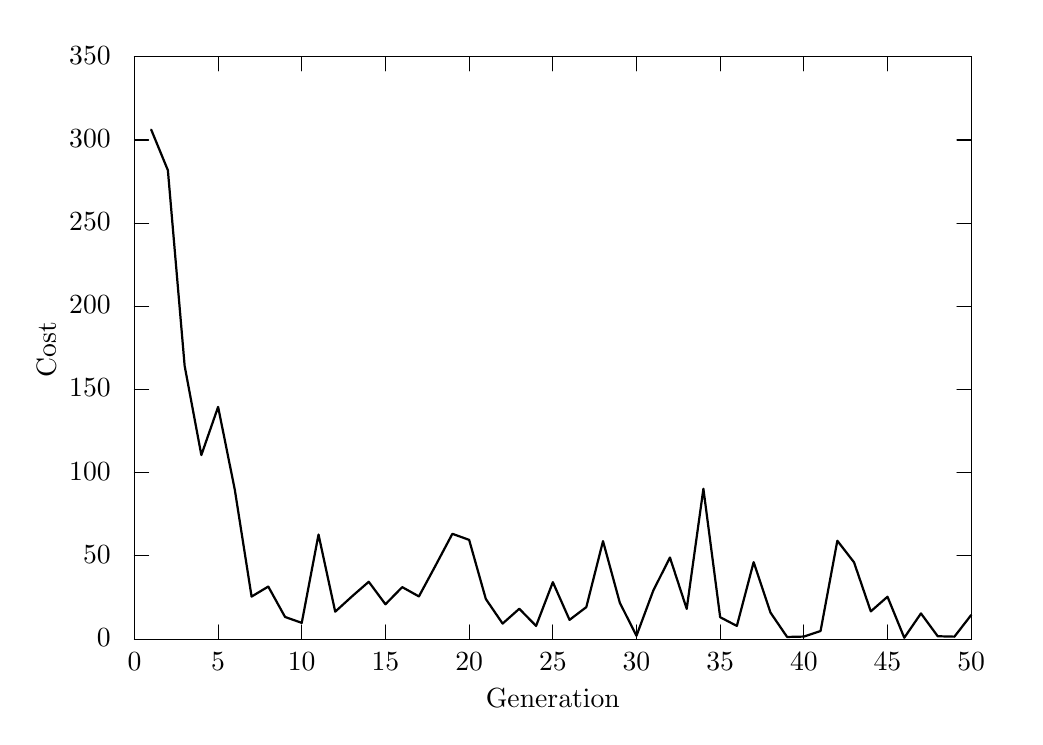
\begin{tikzpicture}[gnuplot]
%% generated with GNUPLOT 5.0p3 (Lua 5.1; terminal rev. 99, script rev. 100)
%% Thu 29 Mar 2018 12:41:20 AM EDT
\gpmonochromelines
\path (0.000,0.000) rectangle (12.500,8.750);
\gpcolor{color=gp lt color border}
\gpsetlinetype{gp lt border}
\gpsetdashtype{gp dt solid}
\gpsetlinewidth{1.00}
\draw[gp path] (1.320,0.985)--(1.500,0.985);
\draw[gp path] (11.947,0.985)--(11.767,0.985);
\node[gp node right] at (1.136,0.985) {$0$};
\draw[gp path] (1.320,2.042)--(1.500,2.042);
\draw[gp path] (11.947,2.042)--(11.767,2.042);
\node[gp node right] at (1.136,2.042) {$50$};
\draw[gp path] (1.320,3.098)--(1.500,3.098);
\draw[gp path] (11.947,3.098)--(11.767,3.098);
\node[gp node right] at (1.136,3.098) {$100$};
\draw[gp path] (1.320,4.155)--(1.500,4.155);
\draw[gp path] (11.947,4.155)--(11.767,4.155);
\node[gp node right] at (1.136,4.155) {$150$};
\draw[gp path] (1.320,5.211)--(1.500,5.211);
\draw[gp path] (11.947,5.211)--(11.767,5.211);
\node[gp node right] at (1.136,5.211) {$200$};
\draw[gp path] (1.320,6.268)--(1.500,6.268);
\draw[gp path] (11.947,6.268)--(11.767,6.268);
\node[gp node right] at (1.136,6.268) {$250$};
\draw[gp path] (1.320,7.324)--(1.500,7.324);
\draw[gp path] (11.947,7.324)--(11.767,7.324);
\node[gp node right] at (1.136,7.324) {$300$};
\draw[gp path] (1.320,8.381)--(1.500,8.381);
\draw[gp path] (11.947,8.381)--(11.767,8.381);
\node[gp node right] at (1.136,8.381) {$350$};
\draw[gp path] (1.320,0.985)--(1.320,1.165);
\draw[gp path] (1.320,8.381)--(1.320,8.201);
\node[gp node center] at (1.320,0.677) {$0$};
\draw[gp path] (2.383,0.985)--(2.383,1.165);
\draw[gp path] (2.383,8.381)--(2.383,8.201);
\node[gp node center] at (2.383,0.677) {$5$};
\draw[gp path] (3.445,0.985)--(3.445,1.165);
\draw[gp path] (3.445,8.381)--(3.445,8.201);
\node[gp node center] at (3.445,0.677) {$10$};
\draw[gp path] (4.508,0.985)--(4.508,1.165);
\draw[gp path] (4.508,8.381)--(4.508,8.201);
\node[gp node center] at (4.508,0.677) {$15$};
\draw[gp path] (5.571,0.985)--(5.571,1.165);
\draw[gp path] (5.571,8.381)--(5.571,8.201);
\node[gp node center] at (5.571,0.677) {$20$};
\draw[gp path] (6.634,0.985)--(6.634,1.165);
\draw[gp path] (6.634,8.381)--(6.634,8.201);
\node[gp node center] at (6.634,0.677) {$25$};
\draw[gp path] (7.696,0.985)--(7.696,1.165);
\draw[gp path] (7.696,8.381)--(7.696,8.201);
\node[gp node center] at (7.696,0.677) {$30$};
\draw[gp path] (8.759,0.985)--(8.759,1.165);
\draw[gp path] (8.759,8.381)--(8.759,8.201);
\node[gp node center] at (8.759,0.677) {$35$};
\draw[gp path] (9.822,0.985)--(9.822,1.165);
\draw[gp path] (9.822,8.381)--(9.822,8.201);
\node[gp node center] at (9.822,0.677) {$40$};
\draw[gp path] (10.884,0.985)--(10.884,1.165);
\draw[gp path] (10.884,8.381)--(10.884,8.201);
\node[gp node center] at (10.884,0.677) {$45$};
\draw[gp path] (11.947,0.985)--(11.947,1.165);
\draw[gp path] (11.947,8.381)--(11.947,8.201);
\node[gp node center] at (11.947,0.677) {$50$};
\draw[gp path] (1.320,8.381)--(1.320,0.985)--(11.947,0.985)--(11.947,8.381)--cycle;
\node[gp node center,rotate=-270] at (0.246,4.683) {Cost};
\node[gp node center] at (6.633,0.215) {Generation};
\gpsetlinewidth{2.00}
\draw[gp path] (1.533,7.455)--(1.745,6.939)--(1.958,4.454)--(2.170,3.322)--(2.383,3.934)%
  --(2.595,2.881)--(2.808,1.525)--(3.020,1.652)--(3.233,1.266)--(3.445,1.191)--(3.658,2.313)%
  --(3.870,1.333)--(4.083,1.527)--(4.296,1.713)--(4.508,1.427)--(4.721,1.645)--(4.933,1.527)%
  --(5.146,1.922)--(5.358,2.322)--(5.571,2.245)--(5.783,1.494)--(5.996,1.182)--(6.208,1.370)%
  --(6.421,1.152)--(6.634,1.708)--(6.846,1.229)--(7.059,1.391)--(7.271,2.229)--(7.484,1.448)%
  --(7.696,1.027)--(7.909,1.600)--(8.121,2.021)--(8.334,1.369)--(8.546,2.894)--(8.759,1.263)%
  --(8.971,1.152)--(9.184,1.962)--(9.397,1.323)--(9.609,1.012)--(9.822,1.017)--(10.034,1.088)%
  --(10.247,2.234)--(10.459,1.960)--(10.672,1.337)--(10.884,1.523)--(11.097,1.002)--(11.309,1.311)%
  --(11.522,1.021)--(11.734,1.016)--(11.947,1.291);
\gpsetlinewidth{1.00}
\draw[gp path] (1.320,8.381)--(1.320,0.985)--(11.947,0.985)--(11.947,8.381)--cycle;
%% coordinates of the plot area
\gpdefrectangularnode{gp plot 1}{\pgfpoint{1.320cm}{0.985cm}}{\pgfpoint{11.947cm}{8.381cm}}
\end{tikzpicture}
%% gnuplot variables
}
    \caption{Individual fitness average by generation.}\label{f:popaverage}
\end{figure}

\begin{figure}
    \centering
    \resizebox{0.75\textwidth}{!}{% GNUPLOT: LaTeX picture with Postscript
\begingroup
  \makeatletter
  \providecommand\color[2][]{%
    \GenericError{(gnuplot) \space\space\space\@spaces}{%
      Package color not loaded in conjunction with
      terminal option `colourtext'%
    }{See the gnuplot documentation for explanation.%
    }{Either use 'blacktext' in gnuplot or load the package
      color.sty in LaTeX.}%
    \renewcommand\color[2][]{}%
  }%
  \providecommand\includegraphics[2][]{%
    \GenericError{(gnuplot) \space\space\space\@spaces}{%
      Package graphicx or graphics not loaded%
    }{See the gnuplot documentation for explanation.%
    }{The gnuplot epslatex terminal needs graphicx.sty or graphics.sty.}%
    \renewcommand\includegraphics[2][]{}%
  }%
  \providecommand\rotatebox[2]{#2}%
  \@ifundefined{ifGPcolor}{%
    \newif\ifGPcolor
    \GPcolorfalse
  }{}%
  \@ifundefined{ifGPblacktext}{%
    \newif\ifGPblacktext
    \GPblacktexttrue
  }{}%
  % define a \g@addto@macro without @ in the name:
  \let\gplgaddtomacro\g@addto@macro
  % define empty templates for all commands taking text:
  \gdef\gplbacktext{}%
  \gdef\gplfronttext{}%
  \makeatother
  \ifGPblacktext
    % no textcolor at all
    \def\colorrgb#1{}%
    \def\colorgray#1{}%
  \else
    % gray or color?
    \ifGPcolor
      \def\colorrgb#1{\color[rgb]{#1}}%
      \def\colorgray#1{\color[gray]{#1}}%
      \expandafter\def\csname LTw\endcsname{\color{white}}%
      \expandafter\def\csname LTb\endcsname{\color{black}}%
      \expandafter\def\csname LTa\endcsname{\color{black}}%
      \expandafter\def\csname LT0\endcsname{\color[rgb]{1,0,0}}%
      \expandafter\def\csname LT1\endcsname{\color[rgb]{0,1,0}}%
      \expandafter\def\csname LT2\endcsname{\color[rgb]{0,0,1}}%
      \expandafter\def\csname LT3\endcsname{\color[rgb]{1,0,1}}%
      \expandafter\def\csname LT4\endcsname{\color[rgb]{0,1,1}}%
      \expandafter\def\csname LT5\endcsname{\color[rgb]{1,1,0}}%
      \expandafter\def\csname LT6\endcsname{\color[rgb]{0,0,0}}%
      \expandafter\def\csname LT7\endcsname{\color[rgb]{1,0.3,0}}%
      \expandafter\def\csname LT8\endcsname{\color[rgb]{0.5,0.5,0.5}}%
    \else
      % gray
      \def\colorrgb#1{\color{black}}%
      \def\colorgray#1{\color[gray]{#1}}%
      \expandafter\def\csname LTw\endcsname{\color{white}}%
      \expandafter\def\csname LTb\endcsname{\color{black}}%
      \expandafter\def\csname LTa\endcsname{\color{black}}%
      \expandafter\def\csname LT0\endcsname{\color{black}}%
      \expandafter\def\csname LT1\endcsname{\color{black}}%
      \expandafter\def\csname LT2\endcsname{\color{black}}%
      \expandafter\def\csname LT3\endcsname{\color{black}}%
      \expandafter\def\csname LT4\endcsname{\color{black}}%
      \expandafter\def\csname LT5\endcsname{\color{black}}%
      \expandafter\def\csname LT6\endcsname{\color{black}}%
      \expandafter\def\csname LT7\endcsname{\color{black}}%
      \expandafter\def\csname LT8\endcsname{\color{black}}%
    \fi
  \fi
    \setlength{\unitlength}{0.0500bp}%
    \ifx\gptboxheight\undefined%
      \newlength{\gptboxheight}%
      \newlength{\gptboxwidth}%
      \newsavebox{\gptboxtext}%
    \fi%
    \setlength{\fboxrule}{0.5pt}%
    \setlength{\fboxsep}{1pt}%
\begin{picture}(7200.00,5040.00)%
    \gplgaddtomacro\gplbacktext{%
      \csname LTb\endcsname%
      \put(946,724){\makebox(0,0)[r]{\strut{}$-1$}}%
      \put(946,1732){\makebox(0,0)[r]{\strut{}$-0.5$}}%
      \put(946,2740){\makebox(0,0)[r]{\strut{}$0$}}%
      \put(946,3747){\makebox(0,0)[r]{\strut{}$0.5$}}%
      \put(946,4755){\makebox(0,0)[r]{\strut{}$1$}}%
      \put(1078,484){\makebox(0,0){\strut{}$0$}}%
      \put(1651,484){\makebox(0,0){\strut{}$5$}}%
      \put(2223,484){\makebox(0,0){\strut{}$10$}}%
      \put(2796,484){\makebox(0,0){\strut{}$15$}}%
      \put(3368,484){\makebox(0,0){\strut{}$20$}}%
      \put(3941,484){\makebox(0,0){\strut{}$25$}}%
      \put(4513,484){\makebox(0,0){\strut{}$30$}}%
      \put(5086,484){\makebox(0,0){\strut{}$35$}}%
      \put(5658,484){\makebox(0,0){\strut{}$40$}}%
      \put(6231,484){\makebox(0,0){\strut{}$45$}}%
      \put(6803,484){\makebox(0,0){\strut{}$50$}}%
    }%
    \gplgaddtomacro\gplfronttext{%
      \csname LTb\endcsname%
      \put(176,2739){\rotatebox{-270}{\makebox(0,0){\strut{}Force, N}}}%
      \put(3940,154){\makebox(0,0){\strut{}Time, s}}%
      \put(5816,4602){\makebox(0,0)[r]{\strut{}Hand-tuned Control Force}}%
      \put(5816,4382){\makebox(0,0)[r]{\strut{}GA-tuned Control Force}}%
    }%
    \gplbacktext
    \put(0,0){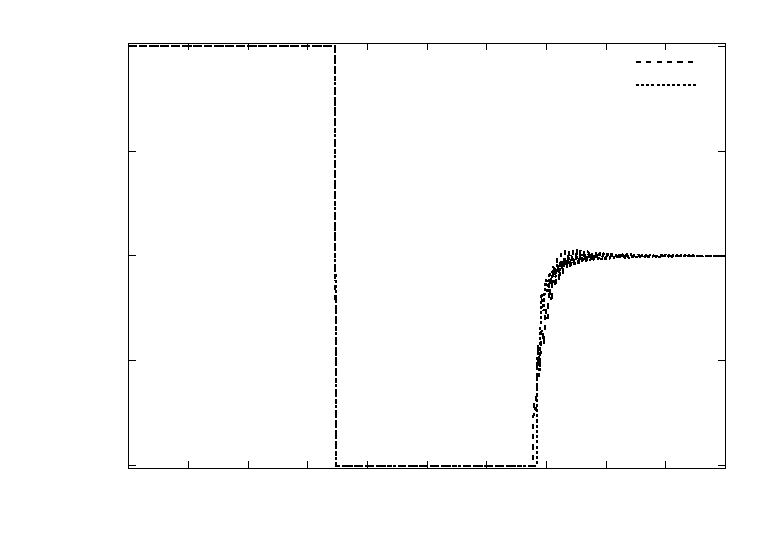
\includegraphics{tikz/accforcecomp}}%
    \gplfronttext
  \end{picture}%
\endgroup
}
    \caption{The force signals over time from the hand- and GA-tuned controllers.}\label{f:accforcecomp}
\end{figure}

\begin{figure}
    \begin{subfigmatrix}{2}
        \subfigure[$x_2$ input partition before GA
        tuning]{\resizebox{0.49\textwidth}{!}{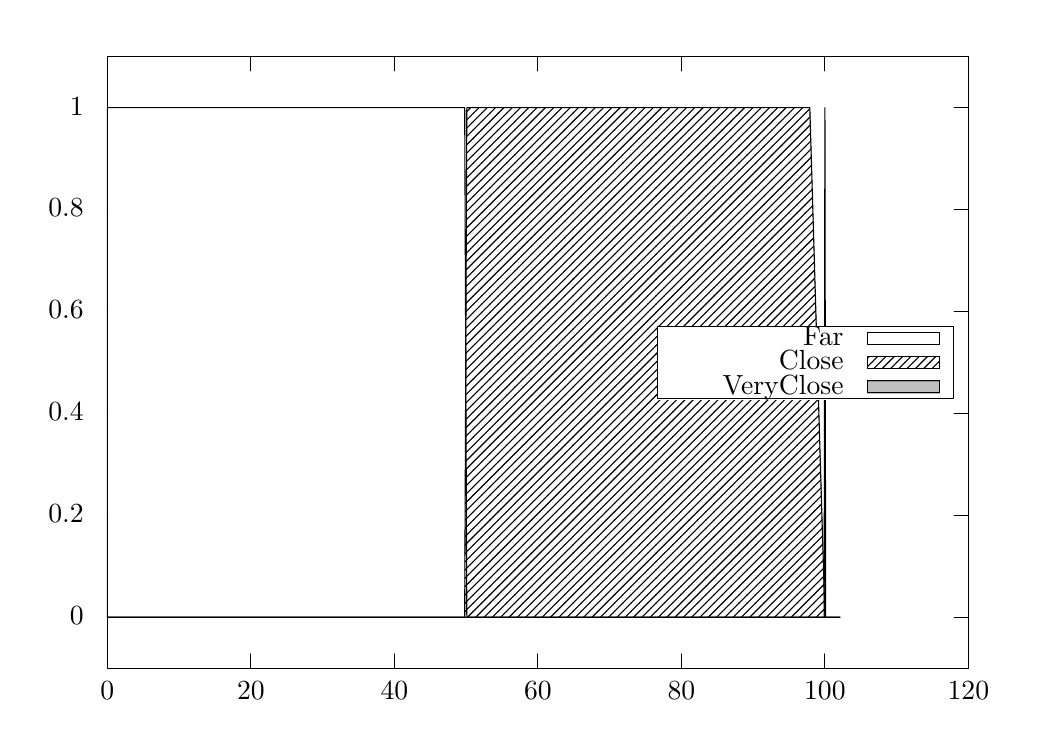
\begin{tikzpicture}[gnuplot]
%% generated with GNUPLOT 5.0p3 (Lua 5.1; terminal rev. 99, script rev. 100)
%% Wed 28 Mar 2018 10:34:02 PM EDT
\gpmonochromelines
\path (0.000,0.000) rectangle (12.500,8.750);
\gpcolor{color=gp lt color border}
\gpsetlinetype{gp lt border}
\gpsetdashtype{gp dt solid}
\gpsetlinewidth{1.00}
\draw[gp path] (1.012,1.263)--(1.192,1.263);
\draw[gp path] (11.947,1.263)--(11.767,1.263);
\node[gp node right] at (0.828,1.263) {$0$};
\draw[gp path] (1.012,2.557)--(1.192,2.557);
\draw[gp path] (11.947,2.557)--(11.767,2.557);
\node[gp node right] at (0.828,2.557) {$0.2$};
\draw[gp path] (1.012,3.851)--(1.192,3.851);
\draw[gp path] (11.947,3.851)--(11.767,3.851);
\node[gp node right] at (0.828,3.851) {$0.4$};
\draw[gp path] (1.012,5.146)--(1.192,5.146);
\draw[gp path] (11.947,5.146)--(11.767,5.146);
\node[gp node right] at (0.828,5.146) {$0.6$};
\draw[gp path] (1.012,6.440)--(1.192,6.440);
\draw[gp path] (11.947,6.440)--(11.767,6.440);
\node[gp node right] at (0.828,6.440) {$0.8$};
\draw[gp path] (1.012,7.734)--(1.192,7.734);
\draw[gp path] (11.947,7.734)--(11.767,7.734);
\node[gp node right] at (0.828,7.734) {$1$};
\draw[gp path] (1.012,0.616)--(1.012,0.796);
\draw[gp path] (1.012,8.381)--(1.012,8.201);
\node[gp node center] at (1.012,0.308) {$0$};
\draw[gp path] (2.835,0.616)--(2.835,0.796);
\draw[gp path] (2.835,8.381)--(2.835,8.201);
\node[gp node center] at (2.835,0.308) {$20$};
\draw[gp path] (4.657,0.616)--(4.657,0.796);
\draw[gp path] (4.657,8.381)--(4.657,8.201);
\node[gp node center] at (4.657,0.308) {$40$};
\draw[gp path] (6.480,0.616)--(6.480,0.796);
\draw[gp path] (6.480,8.381)--(6.480,8.201);
\node[gp node center] at (6.480,0.308) {$60$};
\draw[gp path] (8.302,0.616)--(8.302,0.796);
\draw[gp path] (8.302,8.381)--(8.302,8.201);
\node[gp node center] at (8.302,0.308) {$80$};
\draw[gp path] (10.125,0.616)--(10.125,0.796);
\draw[gp path] (10.125,8.381)--(10.125,8.201);
\node[gp node center] at (10.125,0.308) {$100$};
\draw[gp path] (11.947,0.616)--(11.947,0.796);
\draw[gp path] (11.947,8.381)--(11.947,8.201);
\node[gp node center] at (11.947,0.308) {$120$};
\draw[gp path] (1.012,8.381)--(1.012,0.616)--(11.947,0.616)--(11.947,8.381)--cycle;
\draw[gp path] (7.995,4.036)--(7.995,4.960)--(11.763,4.960)--(11.763,4.036)--cycle;
\gpfill{color=gp lt color border,gp pattern 0,pattern color=.} (1.012,1.263)--(1.012,7.734)--(5.550,7.734)--(5.577,1.263)%
    --(9.933,1.263)--(10.125,1.263)--(10.316,1.263)--cycle;
\draw[gp path] (1.012,1.263)--(1.012,7.734)--(5.550,7.734)--(5.577,1.263)--(9.933,1.263)%
  --(10.125,1.263)--(10.316,1.263);
\gpfill{color=gp lt color border,gp pattern 1,pattern color=.} (1.012,1.263)--(1.012,1.263)--(5.550,1.263)--(5.577,7.734)%
    --(9.933,7.734)--(10.125,1.263)--(10.316,1.263)--cycle;
\gpsetdashtype{gp dt 2}
\draw[gp path] (1.012,1.263)--(5.550,1.263)--(5.577,7.734)--(9.933,7.734)--(10.125,1.263)%
  --(10.316,1.263);
\gpfill{color=gp lt color border,opacity=0.25} (1.012,1.263)--(1.012,1.263)--(5.550,1.263)--(5.577,1.263)%
    --(10.115,1.263)--(10.125,7.734)--(10.134,1.263)--cycle;
\gpsetdashtype{gp dt 3}
\draw[gp path] (1.012,1.263)--(5.550,1.263)--(5.577,1.263)--(10.115,1.263)--(10.125,7.734)%
  --(10.134,1.263);
\gpfill{color=gpbgfillcolor} (7.995,4.036)--(11.763,4.036)--(11.763,4.960)--(7.995,4.960)--cycle;
\gpsetdashtype{gp dt solid}
\draw[gp path] (7.995,4.036)--(7.995,4.960)--(11.763,4.960)--(11.763,4.036)--cycle;
\node[gp node right] at (10.479,4.806) {Far};
\gpfill{color=gp lt color border,gp pattern 0,pattern color=.} (10.663,4.729)--(11.579,4.729)--(11.579,4.883)--(10.663,4.883)--cycle;
\draw[gp path] (10.663,4.729)--(11.579,4.729)--(11.579,4.883)--(10.663,4.883)--cycle;
\node[gp node right] at (10.479,4.498) {Close};
\gpfill{color=gp lt color border,gp pattern 1,pattern color=.} (10.663,4.421)--(11.579,4.421)--(11.579,4.575)--(10.663,4.575)--cycle;
\gpsetdashtype{gp dt 2}
\draw[gp path] (10.663,4.421)--(11.579,4.421)--(11.579,4.575)--(10.663,4.575)--cycle;
\node[gp node right] at (10.479,4.190) {VeryClose};
\gpfill{color=gp lt color border,opacity=0.25} (10.663,4.113)--(11.579,4.113)--(11.579,4.267)--(10.663,4.267)--cycle;
\gpsetdashtype{gp dt 3}
\draw[gp path] (10.663,4.113)--(11.579,4.113)--(11.579,4.267)--(10.663,4.267)--cycle;
\gpsetdashtype{gp dt solid}
\draw[gp path] (1.012,8.381)--(1.012,0.616)--(11.947,0.616)--(11.947,8.381)--cycle;
%% coordinates of the plot area
\gpdefrectangularnode{gp plot 1}{\pgfpoint{1.012cm}{0.616cm}}{\pgfpoint{11.947cm}{8.381cm}}
\end{tikzpicture}
%% gnuplot variables
}}
        \subfigure[$x_2$ input partition after GA
        tuning]{\resizebox{0.49\textwidth}{!}{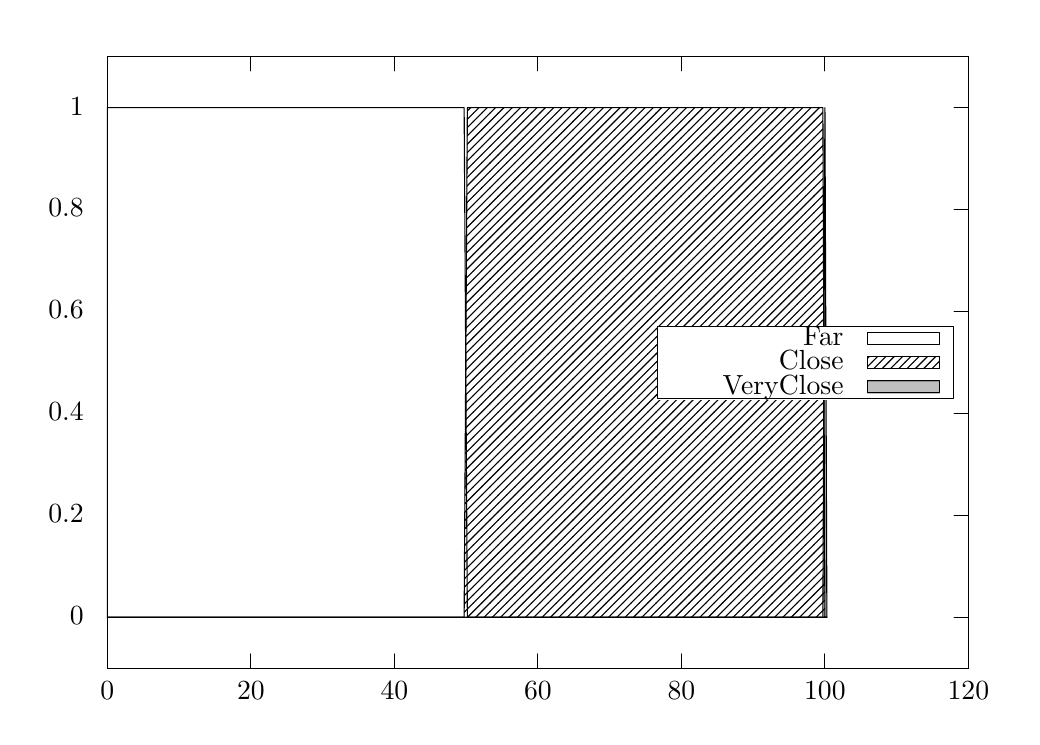
\begin{tikzpicture}[gnuplot]
%% generated with GNUPLOT 5.0p3 (Lua 5.1; terminal rev. 99, script rev. 100)
%% Wed 28 Mar 2018 07:50:11 PM EDT
\gpmonochromelines
\path (0.000,0.000) rectangle (12.500,8.750);
\gpcolor{color=gp lt color border}
\gpsetlinetype{gp lt border}
\gpsetdashtype{gp dt solid}
\gpsetlinewidth{1.00}
\draw[gp path] (1.012,1.263)--(1.192,1.263);
\draw[gp path] (11.947,1.263)--(11.767,1.263);
\node[gp node right] at (0.828,1.263) {$0$};
\draw[gp path] (1.012,2.557)--(1.192,2.557);
\draw[gp path] (11.947,2.557)--(11.767,2.557);
\node[gp node right] at (0.828,2.557) {$0.2$};
\draw[gp path] (1.012,3.851)--(1.192,3.851);
\draw[gp path] (11.947,3.851)--(11.767,3.851);
\node[gp node right] at (0.828,3.851) {$0.4$};
\draw[gp path] (1.012,5.146)--(1.192,5.146);
\draw[gp path] (11.947,5.146)--(11.767,5.146);
\node[gp node right] at (0.828,5.146) {$0.6$};
\draw[gp path] (1.012,6.440)--(1.192,6.440);
\draw[gp path] (11.947,6.440)--(11.767,6.440);
\node[gp node right] at (0.828,6.440) {$0.8$};
\draw[gp path] (1.012,7.734)--(1.192,7.734);
\draw[gp path] (11.947,7.734)--(11.767,7.734);
\node[gp node right] at (0.828,7.734) {$1$};
\draw[gp path] (1.012,0.616)--(1.012,0.796);
\draw[gp path] (1.012,8.381)--(1.012,8.201);
\node[gp node center] at (1.012,0.308) {$0$};
\draw[gp path] (2.835,0.616)--(2.835,0.796);
\draw[gp path] (2.835,8.381)--(2.835,8.201);
\node[gp node center] at (2.835,0.308) {$20$};
\draw[gp path] (4.657,0.616)--(4.657,0.796);
\draw[gp path] (4.657,8.381)--(4.657,8.201);
\node[gp node center] at (4.657,0.308) {$40$};
\draw[gp path] (6.480,0.616)--(6.480,0.796);
\draw[gp path] (6.480,8.381)--(6.480,8.201);
\node[gp node center] at (6.480,0.308) {$60$};
\draw[gp path] (8.302,0.616)--(8.302,0.796);
\draw[gp path] (8.302,8.381)--(8.302,8.201);
\node[gp node center] at (8.302,0.308) {$80$};
\draw[gp path] (10.125,0.616)--(10.125,0.796);
\draw[gp path] (10.125,8.381)--(10.125,8.201);
\node[gp node center] at (10.125,0.308) {$100$};
\draw[gp path] (11.947,0.616)--(11.947,0.796);
\draw[gp path] (11.947,8.381)--(11.947,8.201);
\node[gp node center] at (11.947,0.308) {$120$};
\draw[gp path] (1.012,8.381)--(1.012,0.616)--(11.947,0.616)--(11.947,8.381)--cycle;
\draw[gp path] (7.995,4.036)--(7.995,4.960)--(11.763,4.960)--(11.763,4.036)--cycle;
\gpfill{color=gp lt color border,gp pattern 0,pattern color=.} (1.012,1.263)--(1.012,7.734)--(5.543,7.734)--(5.584,1.263)%
    --(10.099,1.263)--(10.125,1.263)--(10.150,1.263)--cycle;
\draw[gp path] (1.012,1.263)--(1.012,7.734)--(5.543,7.734)--(5.584,1.263)--(10.099,1.263)%
  --(10.125,1.263)--(10.150,1.263);
\gpfill{color=gp lt color border,gp pattern 1,pattern color=.} (1.012,1.263)--(1.012,1.263)--(5.543,1.263)--(5.584,7.734)%
    --(10.099,7.734)--(10.125,1.263)--(10.150,1.263)--cycle;
\gpsetdashtype{gp dt 2}
\draw[gp path] (1.012,1.263)--(5.543,1.263)--(5.584,7.734)--(10.099,7.734)--(10.125,1.263)%
  --(10.150,1.263);
\gpfill{color=gp lt color border,opacity=0.25} (1.012,1.263)--(1.012,1.263)--(5.543,1.263)--(5.584,1.263)%
    --(10.099,1.263)--(10.125,7.734)--(10.150,1.263)--cycle;
\gpsetdashtype{gp dt 3}
\draw[gp path] (1.012,1.263)--(5.543,1.263)--(5.584,1.263)--(10.099,1.263)--(10.125,7.734)%
  --(10.150,1.263);
\gpfill{color=gpbgfillcolor} (7.995,4.036)--(11.763,4.036)--(11.763,4.960)--(7.995,4.960)--cycle;
\gpsetdashtype{gp dt solid}
\draw[gp path] (7.995,4.036)--(7.995,4.960)--(11.763,4.960)--(11.763,4.036)--cycle;
\node[gp node right] at (10.479,4.806) {Far};
\gpfill{color=gp lt color border,gp pattern 0,pattern color=.} (10.663,4.729)--(11.579,4.729)--(11.579,4.883)--(10.663,4.883)--cycle;
\draw[gp path] (10.663,4.729)--(11.579,4.729)--(11.579,4.883)--(10.663,4.883)--cycle;
\node[gp node right] at (10.479,4.498) {Close};
\gpfill{color=gp lt color border,gp pattern 1,pattern color=.} (10.663,4.421)--(11.579,4.421)--(11.579,4.575)--(10.663,4.575)--cycle;
\gpsetdashtype{gp dt 2}
\draw[gp path] (10.663,4.421)--(11.579,4.421)--(11.579,4.575)--(10.663,4.575)--cycle;
\node[gp node right] at (10.479,4.190) {VeryClose};
\gpfill{color=gp lt color border,opacity=0.25} (10.663,4.113)--(11.579,4.113)--(11.579,4.267)--(10.663,4.267)--cycle;
\gpsetdashtype{gp dt 3}
\draw[gp path] (10.663,4.113)--(11.579,4.113)--(11.579,4.267)--(10.663,4.267)--cycle;
\gpsetdashtype{gp dt solid}
\draw[gp path] (1.012,8.381)--(1.012,0.616)--(11.947,0.616)--(11.947,8.381)--cycle;
%% coordinates of the plot area
\gpdefrectangularnode{gp plot 1}{\pgfpoint{1.012cm}{0.616cm}}{\pgfpoint{11.947cm}{8.381cm}}
\end{tikzpicture}
%% gnuplot variables
}}
        \subfigure[$\dot{x}_2$ input partition before GA
        tuning]{\resizebox{0.49\textwidth}{!}{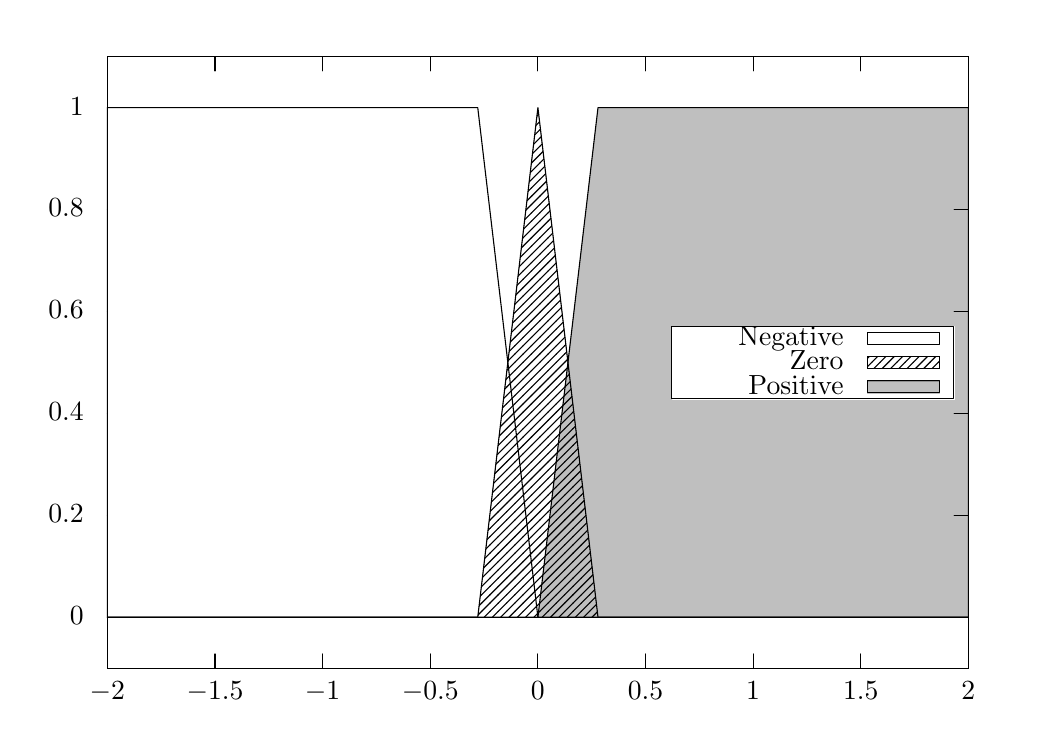
\begin{tikzpicture}[gnuplot]
%% generated with GNUPLOT 5.0p3 (Lua 5.1; terminal rev. 99, script rev. 100)
%% Wed 28 Mar 2018 10:34:02 PM EDT
\gpmonochromelines
\path (0.000,0.000) rectangle (12.500,8.750);
\gpcolor{color=gp lt color border}
\gpsetlinetype{gp lt border}
\gpsetdashtype{gp dt solid}
\gpsetlinewidth{1.00}
\draw[gp path] (1.012,1.263)--(1.192,1.263);
\draw[gp path] (11.947,1.263)--(11.767,1.263);
\node[gp node right] at (0.828,1.263) {$0$};
\draw[gp path] (1.012,2.557)--(1.192,2.557);
\draw[gp path] (11.947,2.557)--(11.767,2.557);
\node[gp node right] at (0.828,2.557) {$0.2$};
\draw[gp path] (1.012,3.851)--(1.192,3.851);
\draw[gp path] (11.947,3.851)--(11.767,3.851);
\node[gp node right] at (0.828,3.851) {$0.4$};
\draw[gp path] (1.012,5.146)--(1.192,5.146);
\draw[gp path] (11.947,5.146)--(11.767,5.146);
\node[gp node right] at (0.828,5.146) {$0.6$};
\draw[gp path] (1.012,6.440)--(1.192,6.440);
\draw[gp path] (11.947,6.440)--(11.767,6.440);
\node[gp node right] at (0.828,6.440) {$0.8$};
\draw[gp path] (1.012,7.734)--(1.192,7.734);
\draw[gp path] (11.947,7.734)--(11.767,7.734);
\node[gp node right] at (0.828,7.734) {$1$};
\draw[gp path] (1.012,0.616)--(1.012,0.796);
\draw[gp path] (1.012,8.381)--(1.012,8.201);
\node[gp node center] at (1.012,0.308) {$-2$};
\draw[gp path] (2.379,0.616)--(2.379,0.796);
\draw[gp path] (2.379,8.381)--(2.379,8.201);
\node[gp node center] at (2.379,0.308) {$-1.5$};
\draw[gp path] (3.746,0.616)--(3.746,0.796);
\draw[gp path] (3.746,8.381)--(3.746,8.201);
\node[gp node center] at (3.746,0.308) {$-1$};
\draw[gp path] (5.113,0.616)--(5.113,0.796);
\draw[gp path] (5.113,8.381)--(5.113,8.201);
\node[gp node center] at (5.113,0.308) {$-0.5$};
\draw[gp path] (6.480,0.616)--(6.480,0.796);
\draw[gp path] (6.480,8.381)--(6.480,8.201);
\node[gp node center] at (6.480,0.308) {$0$};
\draw[gp path] (7.846,0.616)--(7.846,0.796);
\draw[gp path] (7.846,8.381)--(7.846,8.201);
\node[gp node center] at (7.846,0.308) {$0.5$};
\draw[gp path] (9.213,0.616)--(9.213,0.796);
\draw[gp path] (9.213,8.381)--(9.213,8.201);
\node[gp node center] at (9.213,0.308) {$1$};
\draw[gp path] (10.580,0.616)--(10.580,0.796);
\draw[gp path] (10.580,8.381)--(10.580,8.201);
\node[gp node center] at (10.580,0.308) {$1.5$};
\draw[gp path] (11.947,0.616)--(11.947,0.796);
\draw[gp path] (11.947,8.381)--(11.947,8.201);
\node[gp node center] at (11.947,0.308) {$2$};
\draw[gp path] (1.012,8.381)--(1.012,0.616)--(11.947,0.616)--(11.947,8.381)--cycle;
\draw[gp path] (8.179,4.036)--(8.179,4.960)--(11.763,4.960)--(11.763,4.036)--cycle;
\gpfill{color=gp lt color border,gp pattern 0,pattern color=.} (1.012,1.263)--(1.012,7.734)--(5.716,7.734)--(6.480,1.263)%
    --(7.243,1.263)--(11.947,1.263)--(11.947,1.263)--cycle;
\draw[gp path] (1.012,1.263)--(1.012,7.734)--(5.716,7.734)--(6.480,1.263)--(7.243,1.263)%
  --(11.947,1.263);
\gpfill{color=gp lt color border,gp pattern 1,pattern color=.} (1.012,1.263)--(1.012,1.263)--(5.716,1.263)--(6.480,7.734)%
    --(7.243,1.263)--(11.947,1.263)--(11.947,1.263)--cycle;
\gpsetdashtype{gp dt 2}
\draw[gp path] (1.012,1.263)--(5.716,1.263)--(6.480,7.734)--(7.243,1.263)--(11.947,1.263);
\gpfill{color=gp lt color border,opacity=0.25} (1.012,1.263)--(1.012,1.263)--(5.716,1.263)--(6.480,1.263)%
    --(7.243,7.734)--(11.947,7.734)--(11.947,1.263)--cycle;
\gpsetdashtype{gp dt 3}
\draw[gp path] (1.012,1.263)--(5.716,1.263)--(6.480,1.263)--(7.243,7.734)--(11.947,7.734)%
  --(11.947,1.263);
\gpfill{color=gpbgfillcolor} (8.179,4.036)--(11.763,4.036)--(11.763,4.960)--(8.179,4.960)--cycle;
\gpsetdashtype{gp dt solid}
\draw[gp path] (8.179,4.036)--(8.179,4.960)--(11.763,4.960)--(11.763,4.036)--cycle;
\node[gp node right] at (10.479,4.806) {Negative};
\gpfill{color=gp lt color border,gp pattern 0,pattern color=.} (10.663,4.729)--(11.579,4.729)--(11.579,4.883)--(10.663,4.883)--cycle;
\draw[gp path] (10.663,4.729)--(11.579,4.729)--(11.579,4.883)--(10.663,4.883)--cycle;
\node[gp node right] at (10.479,4.498) {Zero};
\gpfill{color=gp lt color border,gp pattern 1,pattern color=.} (10.663,4.421)--(11.579,4.421)--(11.579,4.575)--(10.663,4.575)--cycle;
\gpsetdashtype{gp dt 2}
\draw[gp path] (10.663,4.421)--(11.579,4.421)--(11.579,4.575)--(10.663,4.575)--cycle;
\node[gp node right] at (10.479,4.190) {Positive};
\gpfill{color=gp lt color border,opacity=0.25} (10.663,4.113)--(11.579,4.113)--(11.579,4.267)--(10.663,4.267)--cycle;
\gpsetdashtype{gp dt 3}
\draw[gp path] (10.663,4.113)--(11.579,4.113)--(11.579,4.267)--(10.663,4.267)--cycle;
\gpsetdashtype{gp dt solid}
\draw[gp path] (1.012,8.381)--(1.012,0.616)--(11.947,0.616)--(11.947,8.381)--cycle;
%% coordinates of the plot area
\gpdefrectangularnode{gp plot 1}{\pgfpoint{1.012cm}{0.616cm}}{\pgfpoint{11.947cm}{8.381cm}}
\end{tikzpicture}
%% gnuplot variables
}}
        \subfigure[$\dot{x}_2$ input partition after GA
        tuning]{\resizebox{0.49\textwidth}{!}{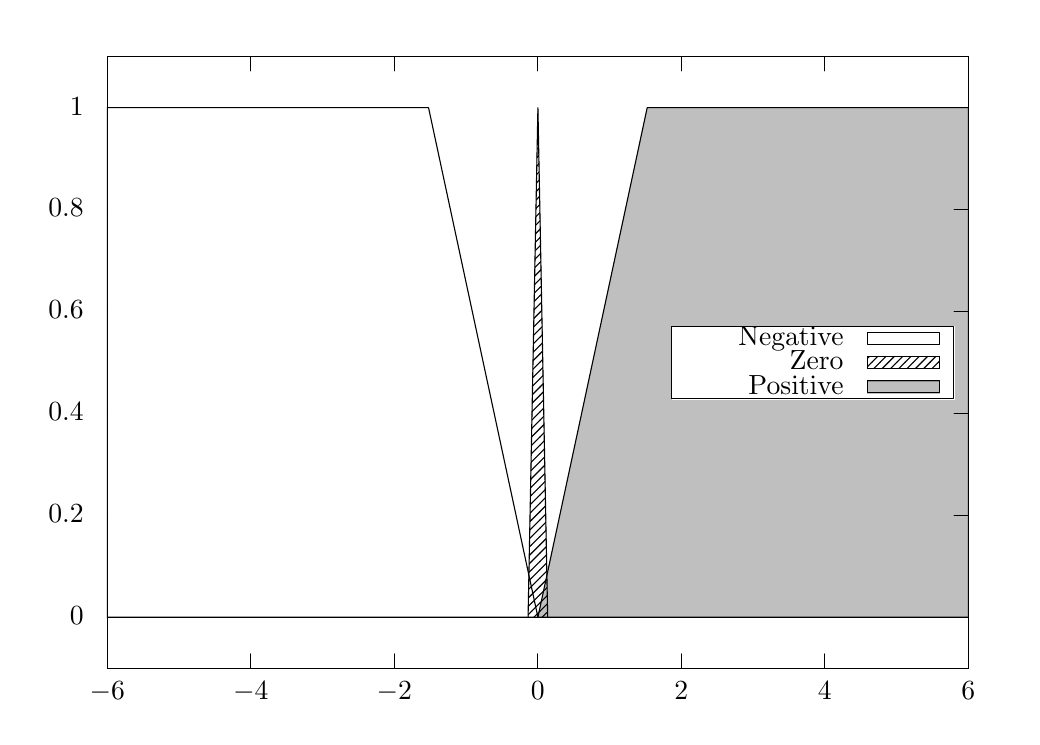
\begin{tikzpicture}[gnuplot]
%% generated with GNUPLOT 5.0p3 (Lua 5.1; terminal rev. 99, script rev. 100)
%% Wed 28 Mar 2018 07:50:11 PM EDT
\gpmonochromelines
\path (0.000,0.000) rectangle (12.500,8.750);
\gpcolor{color=gp lt color border}
\gpsetlinetype{gp lt border}
\gpsetdashtype{gp dt solid}
\gpsetlinewidth{1.00}
\draw[gp path] (1.012,1.263)--(1.192,1.263);
\draw[gp path] (11.947,1.263)--(11.767,1.263);
\node[gp node right] at (0.828,1.263) {$0$};
\draw[gp path] (1.012,2.557)--(1.192,2.557);
\draw[gp path] (11.947,2.557)--(11.767,2.557);
\node[gp node right] at (0.828,2.557) {$0.2$};
\draw[gp path] (1.012,3.851)--(1.192,3.851);
\draw[gp path] (11.947,3.851)--(11.767,3.851);
\node[gp node right] at (0.828,3.851) {$0.4$};
\draw[gp path] (1.012,5.146)--(1.192,5.146);
\draw[gp path] (11.947,5.146)--(11.767,5.146);
\node[gp node right] at (0.828,5.146) {$0.6$};
\draw[gp path] (1.012,6.440)--(1.192,6.440);
\draw[gp path] (11.947,6.440)--(11.767,6.440);
\node[gp node right] at (0.828,6.440) {$0.8$};
\draw[gp path] (1.012,7.734)--(1.192,7.734);
\draw[gp path] (11.947,7.734)--(11.767,7.734);
\node[gp node right] at (0.828,7.734) {$1$};
\draw[gp path] (1.012,0.616)--(1.012,0.796);
\draw[gp path] (1.012,8.381)--(1.012,8.201);
\node[gp node center] at (1.012,0.308) {$-6$};
\draw[gp path] (2.835,0.616)--(2.835,0.796);
\draw[gp path] (2.835,8.381)--(2.835,8.201);
\node[gp node center] at (2.835,0.308) {$-4$};
\draw[gp path] (4.657,0.616)--(4.657,0.796);
\draw[gp path] (4.657,8.381)--(4.657,8.201);
\node[gp node center] at (4.657,0.308) {$-2$};
\draw[gp path] (6.480,0.616)--(6.480,0.796);
\draw[gp path] (6.480,8.381)--(6.480,8.201);
\node[gp node center] at (6.480,0.308) {$0$};
\draw[gp path] (8.302,0.616)--(8.302,0.796);
\draw[gp path] (8.302,8.381)--(8.302,8.201);
\node[gp node center] at (8.302,0.308) {$2$};
\draw[gp path] (10.125,0.616)--(10.125,0.796);
\draw[gp path] (10.125,8.381)--(10.125,8.201);
\node[gp node center] at (10.125,0.308) {$4$};
\draw[gp path] (11.947,0.616)--(11.947,0.796);
\draw[gp path] (11.947,8.381)--(11.947,8.201);
\node[gp node center] at (11.947,0.308) {$6$};
\draw[gp path] (1.012,8.381)--(1.012,0.616)--(11.947,0.616)--(11.947,8.381)--cycle;
\draw[gp path] (8.179,4.036)--(8.179,4.960)--(11.763,4.960)--(11.763,4.036)--cycle;
\gpfill{color=gp lt color border,gp pattern 0,pattern color=.} (1.012,1.263)--(1.012,7.734)--(5.091,7.734)--(6.480,1.263)%
    --(7.868,1.263)--(11.947,1.263)--(11.947,1.263)--cycle;
\draw[gp path] (1.012,1.263)--(1.012,7.734)--(5.091,7.734)--(6.480,1.263)--(7.868,1.263)%
  --(11.947,1.263);
\gpfill{color=gp lt color border,gp pattern 1,pattern color=.} (6.355,1.263)--(6.480,7.734)--(6.604,1.263)--cycle;
\gpsetdashtype{gp dt 2}
\draw[gp path] (6.355,1.263)--(6.480,7.734)--(6.604,1.263);
\gpfill{color=gp lt color border,opacity=0.25} (1.012,1.263)--(1.012,1.263)--(5.091,1.263)--(6.480,1.263)%
    --(7.868,7.734)--(11.947,7.734)--(11.947,1.263)--cycle;
\gpsetdashtype{gp dt 3}
\draw[gp path] (1.012,1.263)--(5.091,1.263)--(6.480,1.263)--(7.868,7.734)--(11.947,7.734)%
  --(11.947,1.263);
\gpfill{color=gpbgfillcolor} (8.179,4.036)--(11.763,4.036)--(11.763,4.960)--(8.179,4.960)--cycle;
\gpsetdashtype{gp dt solid}
\draw[gp path] (8.179,4.036)--(8.179,4.960)--(11.763,4.960)--(11.763,4.036)--cycle;
\node[gp node right] at (10.479,4.806) {Negative};
\gpfill{color=gp lt color border,gp pattern 0,pattern color=.} (10.663,4.729)--(11.579,4.729)--(11.579,4.883)--(10.663,4.883)--cycle;
\draw[gp path] (10.663,4.729)--(11.579,4.729)--(11.579,4.883)--(10.663,4.883)--cycle;
\node[gp node right] at (10.479,4.498) {Zero};
\gpfill{color=gp lt color border,gp pattern 1,pattern color=.} (10.663,4.421)--(11.579,4.421)--(11.579,4.575)--(10.663,4.575)--cycle;
\gpsetdashtype{gp dt 2}
\draw[gp path] (10.663,4.421)--(11.579,4.421)--(11.579,4.575)--(10.663,4.575)--cycle;
\node[gp node right] at (10.479,4.190) {Positive};
\gpfill{color=gp lt color border,opacity=0.25} (10.663,4.113)--(11.579,4.113)--(11.579,4.267)--(10.663,4.267)--cycle;
\gpsetdashtype{gp dt 3}
\draw[gp path] (10.663,4.113)--(11.579,4.113)--(11.579,4.267)--(10.663,4.267)--cycle;
\gpsetdashtype{gp dt solid}
\draw[gp path] (1.012,8.381)--(1.012,0.616)--(11.947,0.616)--(11.947,8.381)--cycle;
%% coordinates of the plot area
\gpdefrectangularnode{gp plot 1}{\pgfpoint{1.012cm}{0.616cm}}{\pgfpoint{11.947cm}{8.381cm}}
\end{tikzpicture}
%% gnuplot variables
}}
        \subfigure[Force output partition before GA
        tuning]{\resizebox{0.49\textwidth}{!}{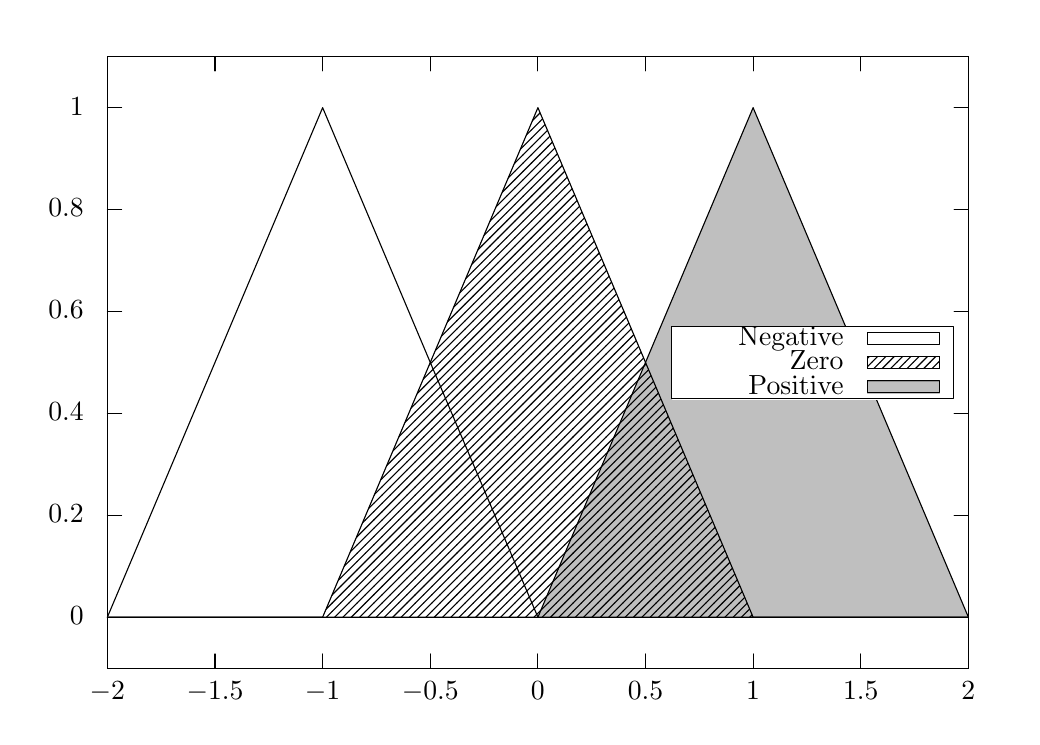
\begin{tikzpicture}[gnuplot]
%% generated with GNUPLOT 5.0p3 (Lua 5.1; terminal rev. 99, script rev. 100)
%% Wed 28 Mar 2018 10:34:02 PM EDT
\gpmonochromelines
\path (0.000,0.000) rectangle (12.500,8.750);
\gpcolor{color=gp lt color border}
\gpsetlinetype{gp lt border}
\gpsetdashtype{gp dt solid}
\gpsetlinewidth{1.00}
\draw[gp path] (1.012,1.263)--(1.192,1.263);
\draw[gp path] (11.947,1.263)--(11.767,1.263);
\node[gp node right] at (0.828,1.263) {$0$};
\draw[gp path] (1.012,2.557)--(1.192,2.557);
\draw[gp path] (11.947,2.557)--(11.767,2.557);
\node[gp node right] at (0.828,2.557) {$0.2$};
\draw[gp path] (1.012,3.851)--(1.192,3.851);
\draw[gp path] (11.947,3.851)--(11.767,3.851);
\node[gp node right] at (0.828,3.851) {$0.4$};
\draw[gp path] (1.012,5.146)--(1.192,5.146);
\draw[gp path] (11.947,5.146)--(11.767,5.146);
\node[gp node right] at (0.828,5.146) {$0.6$};
\draw[gp path] (1.012,6.440)--(1.192,6.440);
\draw[gp path] (11.947,6.440)--(11.767,6.440);
\node[gp node right] at (0.828,6.440) {$0.8$};
\draw[gp path] (1.012,7.734)--(1.192,7.734);
\draw[gp path] (11.947,7.734)--(11.767,7.734);
\node[gp node right] at (0.828,7.734) {$1$};
\draw[gp path] (1.012,0.616)--(1.012,0.796);
\draw[gp path] (1.012,8.381)--(1.012,8.201);
\node[gp node center] at (1.012,0.308) {$-2$};
\draw[gp path] (2.379,0.616)--(2.379,0.796);
\draw[gp path] (2.379,8.381)--(2.379,8.201);
\node[gp node center] at (2.379,0.308) {$-1.5$};
\draw[gp path] (3.746,0.616)--(3.746,0.796);
\draw[gp path] (3.746,8.381)--(3.746,8.201);
\node[gp node center] at (3.746,0.308) {$-1$};
\draw[gp path] (5.113,0.616)--(5.113,0.796);
\draw[gp path] (5.113,8.381)--(5.113,8.201);
\node[gp node center] at (5.113,0.308) {$-0.5$};
\draw[gp path] (6.480,0.616)--(6.480,0.796);
\draw[gp path] (6.480,8.381)--(6.480,8.201);
\node[gp node center] at (6.480,0.308) {$0$};
\draw[gp path] (7.846,0.616)--(7.846,0.796);
\draw[gp path] (7.846,8.381)--(7.846,8.201);
\node[gp node center] at (7.846,0.308) {$0.5$};
\draw[gp path] (9.213,0.616)--(9.213,0.796);
\draw[gp path] (9.213,8.381)--(9.213,8.201);
\node[gp node center] at (9.213,0.308) {$1$};
\draw[gp path] (10.580,0.616)--(10.580,0.796);
\draw[gp path] (10.580,8.381)--(10.580,8.201);
\node[gp node center] at (10.580,0.308) {$1.5$};
\draw[gp path] (11.947,0.616)--(11.947,0.796);
\draw[gp path] (11.947,8.381)--(11.947,8.201);
\node[gp node center] at (11.947,0.308) {$2$};
\draw[gp path] (1.012,8.381)--(1.012,0.616)--(11.947,0.616)--(11.947,8.381)--cycle;
\draw[gp path] (8.179,4.036)--(8.179,4.960)--(11.763,4.960)--(11.763,4.036)--cycle;
%
  \gpfill{color=gp lt color border,gp pattern 0,pattern color=.} (1.012,1.263)--(3.746,7.734)--(6.480,1.263)--(9.213,1.263)--(11.947,1.263)--cycle;
\draw[gp path] (1.012,1.263)--(3.746,7.734)--(6.480,1.263)--(9.213,1.263)--(11.947,1.263);
%
  \gpfill{color=gp lt color border,gp pattern 1,pattern color=.} (1.012,1.263)--(3.746,1.263)--(6.480,7.734)--(9.213,1.263)--(11.947,1.263)--cycle;
\gpsetdashtype{gp dt 2}
\draw[gp path] (1.012,1.263)--(3.746,1.263)--(6.480,7.734)--(9.213,1.263)--(11.947,1.263);
%
  \gpfill{color=gp lt color border,opacity=0.25} (1.012,1.263)--(3.746,1.263)--(6.480,1.263)--(9.213,7.734)--(11.947,1.263)--cycle;
\gpsetdashtype{gp dt 3}
\draw[gp path] (1.012,1.263)--(3.746,1.263)--(6.480,1.263)--(9.213,7.734)--(11.947,1.263);
\gpfill{color=gpbgfillcolor} (8.179,4.036)--(11.763,4.036)--(11.763,4.960)--(8.179,4.960)--cycle;
\gpsetdashtype{gp dt solid}
\draw[gp path] (8.179,4.036)--(8.179,4.960)--(11.763,4.960)--(11.763,4.036)--cycle;
\node[gp node right] at (10.479,4.806) {Negative};
\gpfill{color=gp lt color border,gp pattern 0,pattern color=.} (10.663,4.729)--(11.579,4.729)--(11.579,4.883)--(10.663,4.883)--cycle;
\draw[gp path] (10.663,4.729)--(11.579,4.729)--(11.579,4.883)--(10.663,4.883)--cycle;
\node[gp node right] at (10.479,4.498) {Zero};
\gpfill{color=gp lt color border,gp pattern 1,pattern color=.} (10.663,4.421)--(11.579,4.421)--(11.579,4.575)--(10.663,4.575)--cycle;
\gpsetdashtype{gp dt 2}
\draw[gp path] (10.663,4.421)--(11.579,4.421)--(11.579,4.575)--(10.663,4.575)--cycle;
\node[gp node right] at (10.479,4.190) {Positive};
\gpfill{color=gp lt color border,opacity=0.25} (10.663,4.113)--(11.579,4.113)--(11.579,4.267)--(10.663,4.267)--cycle;
\gpsetdashtype{gp dt 3}
\draw[gp path] (10.663,4.113)--(11.579,4.113)--(11.579,4.267)--(10.663,4.267)--cycle;
\gpsetdashtype{gp dt solid}
\draw[gp path] (1.012,8.381)--(1.012,0.616)--(11.947,0.616)--(11.947,8.381)--cycle;
%% coordinates of the plot area
\gpdefrectangularnode{gp plot 1}{\pgfpoint{1.012cm}{0.616cm}}{\pgfpoint{11.947cm}{8.381cm}}
\end{tikzpicture}
%% gnuplot variables
}}
        \subfigure[Force output partition after GA
        tuning]{\resizebox{0.49\textwidth}{!}{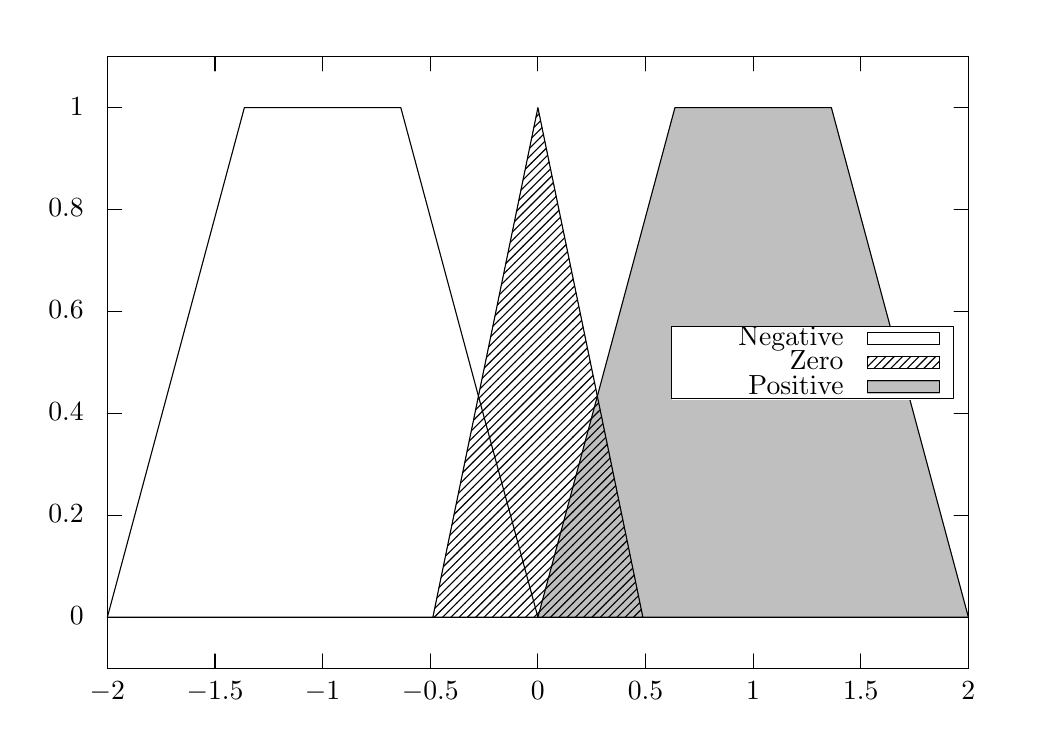
\begin{tikzpicture}[gnuplot]
%% generated with GNUPLOT 5.0p3 (Lua 5.1; terminal rev. 99, script rev. 100)
%% Wed 28 Mar 2018 07:50:11 PM EDT
\gpmonochromelines
\path (0.000,0.000) rectangle (12.500,8.750);
\gpcolor{color=gp lt color border}
\gpsetlinetype{gp lt border}
\gpsetdashtype{gp dt solid}
\gpsetlinewidth{1.00}
\draw[gp path] (1.012,1.263)--(1.192,1.263);
\draw[gp path] (11.947,1.263)--(11.767,1.263);
\node[gp node right] at (0.828,1.263) {$0$};
\draw[gp path] (1.012,2.557)--(1.192,2.557);
\draw[gp path] (11.947,2.557)--(11.767,2.557);
\node[gp node right] at (0.828,2.557) {$0.2$};
\draw[gp path] (1.012,3.851)--(1.192,3.851);
\draw[gp path] (11.947,3.851)--(11.767,3.851);
\node[gp node right] at (0.828,3.851) {$0.4$};
\draw[gp path] (1.012,5.146)--(1.192,5.146);
\draw[gp path] (11.947,5.146)--(11.767,5.146);
\node[gp node right] at (0.828,5.146) {$0.6$};
\draw[gp path] (1.012,6.440)--(1.192,6.440);
\draw[gp path] (11.947,6.440)--(11.767,6.440);
\node[gp node right] at (0.828,6.440) {$0.8$};
\draw[gp path] (1.012,7.734)--(1.192,7.734);
\draw[gp path] (11.947,7.734)--(11.767,7.734);
\node[gp node right] at (0.828,7.734) {$1$};
\draw[gp path] (1.012,0.616)--(1.012,0.796);
\draw[gp path] (1.012,8.381)--(1.012,8.201);
\node[gp node center] at (1.012,0.308) {$-2$};
\draw[gp path] (2.379,0.616)--(2.379,0.796);
\draw[gp path] (2.379,8.381)--(2.379,8.201);
\node[gp node center] at (2.379,0.308) {$-1.5$};
\draw[gp path] (3.746,0.616)--(3.746,0.796);
\draw[gp path] (3.746,8.381)--(3.746,8.201);
\node[gp node center] at (3.746,0.308) {$-1$};
\draw[gp path] (5.113,0.616)--(5.113,0.796);
\draw[gp path] (5.113,8.381)--(5.113,8.201);
\node[gp node center] at (5.113,0.308) {$-0.5$};
\draw[gp path] (6.480,0.616)--(6.480,0.796);
\draw[gp path] (6.480,8.381)--(6.480,8.201);
\node[gp node center] at (6.480,0.308) {$0$};
\draw[gp path] (7.846,0.616)--(7.846,0.796);
\draw[gp path] (7.846,8.381)--(7.846,8.201);
\node[gp node center] at (7.846,0.308) {$0.5$};
\draw[gp path] (9.213,0.616)--(9.213,0.796);
\draw[gp path] (9.213,8.381)--(9.213,8.201);
\node[gp node center] at (9.213,0.308) {$1$};
\draw[gp path] (10.580,0.616)--(10.580,0.796);
\draw[gp path] (10.580,8.381)--(10.580,8.201);
\node[gp node center] at (10.580,0.308) {$1.5$};
\draw[gp path] (11.947,0.616)--(11.947,0.796);
\draw[gp path] (11.947,8.381)--(11.947,8.201);
\node[gp node center] at (11.947,0.308) {$2$};
\draw[gp path] (1.012,8.381)--(1.012,0.616)--(11.947,0.616)--(11.947,8.381)--cycle;
\draw[gp path] (8.179,4.036)--(8.179,4.960)--(11.763,4.960)--(11.763,4.036)--cycle;
\gpfill{color=gp lt color border,gp pattern 0,pattern color=.} (1.012,1.263)--(2.752,7.734)--(4.739,7.734)--(6.480,1.263)%
    --(8.220,1.263)--(10.207,1.263)--(11.947,1.263)--cycle;
\draw[gp path] (1.012,1.263)--(2.752,7.734)--(4.739,7.734)--(6.480,1.263)--(8.220,1.263)%
  --(10.207,1.263)--(11.947,1.263);
\gpfill{color=gp lt color border,gp pattern 1,pattern color=.} (5.146,1.263)--(6.480,7.734)--(7.813,1.263)--cycle;
\gpsetdashtype{gp dt 2}
\draw[gp path] (5.146,1.263)--(6.480,7.734)--(7.813,1.263);
\gpfill{color=gp lt color border,opacity=0.25} (1.012,1.263)--(2.752,1.263)--(4.739,1.263)--(6.480,1.263)%
    --(8.220,7.734)--(10.207,7.734)--(11.947,1.263)--cycle;
\gpsetdashtype{gp dt 3}
\draw[gp path] (1.012,1.263)--(2.752,1.263)--(4.739,1.263)--(6.480,1.263)--(8.220,7.734)%
  --(10.207,7.734)--(11.947,1.263);
\gpfill{color=gpbgfillcolor} (8.179,4.036)--(11.763,4.036)--(11.763,4.960)--(8.179,4.960)--cycle;
\gpsetdashtype{gp dt solid}
\draw[gp path] (8.179,4.036)--(8.179,4.960)--(11.763,4.960)--(11.763,4.036)--cycle;
\node[gp node right] at (10.479,4.806) {Negative};
\gpfill{color=gp lt color border,gp pattern 0,pattern color=.} (10.663,4.729)--(11.579,4.729)--(11.579,4.883)--(10.663,4.883)--cycle;
\draw[gp path] (10.663,4.729)--(11.579,4.729)--(11.579,4.883)--(10.663,4.883)--cycle;
\node[gp node right] at (10.479,4.498) {Zero};
\gpfill{color=gp lt color border,gp pattern 1,pattern color=.} (10.663,4.421)--(11.579,4.421)--(11.579,4.575)--(10.663,4.575)--cycle;
\gpsetdashtype{gp dt 2}
\draw[gp path] (10.663,4.421)--(11.579,4.421)--(11.579,4.575)--(10.663,4.575)--cycle;
\node[gp node right] at (10.479,4.190) {Positive};
\gpfill{color=gp lt color border,opacity=0.25} (10.663,4.113)--(11.579,4.113)--(11.579,4.267)--(10.663,4.267)--cycle;
\gpsetdashtype{gp dt 3}
\draw[gp path] (10.663,4.113)--(11.579,4.113)--(11.579,4.267)--(10.663,4.267)--cycle;
\gpsetdashtype{gp dt solid}
\draw[gp path] (1.012,8.381)--(1.012,0.616)--(11.947,0.616)--(11.947,8.381)--cycle;
%% coordinates of the plot area
\gpdefrectangularnode{gp plot 1}{\pgfpoint{1.012cm}{0.616cm}}{\pgfpoint{11.947cm}{8.381cm}}
\end{tikzpicture}
%% gnuplot variables
}}
    \end{subfigmatrix} \caption{FIS comparison between hand- and GA-tuned membership
    functions}\label{f:fiscomp}
\end{figure}

\subsection{Genetic Adaptability}
These results demonstrate the ability of the genetic algorithm to tune a FIS
to near-optimal performance. All tuning and development heretofore was done with an unchanging system setup of
known masses connected by a known spring. Although a robust controller\cite{cohen:01jgcd}, introducing changes
to the masses of each car significantly alters the performance of the FIS as it was carefully tuned to only a
certain envelope; however, utilizing the genetic algorithm to generate an optimum FIS for each new system
setup is an efficient method of developing good active controllers. This is demonstrated by changing the
masses $m_1$ and $m_2$ to \SI{2}{\kilogram} and \SI{4}{\kilogram} respectively. They are again changed to
\SI{4}{\kilogram} and \SI{8}{\kilogram}, and finally \SI{4}{\kilogram} and \SI{16}{\kilogram}. The algorithm
was deployed for each case to optimize a controller for that envelope. After fifty generations of evolution,
the genetically optimized FIS performed within 3\% of the theoretical rigid body limit in all four cases.
These results are displayed in \cref{tab:gacomp}.  \begin{table} \centering \caption{Genetic algorithm
    FIS performance compared to the hand-tuned FIS and rigid body limit.} \label{tab:gacomp}
    \begin{tabular}{|c|c|c|c|c|} \cline{2-5} \multicolumn{1}{c|}{} & \multicolumn{4}{|c|}{Mass 1
        (\si{\kilogram}), Mass 2 (\si{\kilogram})} \\\cline{2-5} \multicolumn{1}{c|}{} & \SI{1}{\kilogram},
        \SI{2}{\kilogram} & \SI{2}{\kilogram}, \SI{4}{\kilogram} & \SI{4}{\kilogram}, \SI{8}{\kilogram} &
        \SI{4}{\kilogram}, \SI{16}{\kilogram} \\\hline Theoretical Limit & 0.3191 & 0.4553 & 0.6438 & 0.8312
        \\\hline GA FIS & 0.3231 & 0.4562 & 0.6579 & 0.8434 \\\hline Hand-tuned FIS & 0.3233 & 0.6125 & 5.3072
                        & 3.3240 \\\hline\hline GA Error & \multicolumn{1}{|d|}{1.3\%} &
        \multicolumn{1}{|d|}{0.2\%} & \multicolumn{1}{|d|}{2.2\%} & \multicolumn{1}{|d|}{1.5\%} \\\hline
        Hand-tuned Error & \multicolumn{1}{|d|}{1.3\%} & \multicolumn{1}{|d|}{34.5\%} &
        \multicolumn{1}{|d|}{724.4\%} & \multicolumn{1}{|d|}{299.9\%} \\\hline \end{tabular} \end{table}

It is easily seen in these results that the use of the genetic algorithm is advantageous in the autonomous
development of near optimal FIS controllers. Given a generic control architecture, the genetic algorithm is
able to tune a FIS rapidly and accurately for a varied set of circumstances.

\section{Conclusions} Fuzzy logic provides a robust framework for control. It has
been demonstrated that proper fuzzy control is efficient and computationally inexpensive. The inherent
vagueness of set membership and linguistic operation of fuzzy logic allows the controller to mimic expert
human control. This superior control, however, comes with a steep cost in FIS development. Hand-tuning a FIS
is time-consuming and tedious.


The use of the genetic algorithm facilitates FIS development. Once a FIS has been developed for a general type
of control situation, it is relatively simple to define the FIS as a genetic element and automate the tuning
through the evolutionary process. These results imply that if a general fuzzy controller is developed for a
family of control situations, then a genetic algorithm can be implemented to tune each FIS to its specific
task. The tuning, therefore, can be accomplished by someone with no expertise in the control of the situation.
As the computation is quick, efficient control could be widely distributed due also to the low-cost of
development.




\chapter{F-4 Pitch Attitude Control}\label{c:f4}
\section{Introduction} 

This chapter outlines a fuzzy PID system for the approach condition of an F-4 fighter jet. The F4 stands in
for more modern jets with fly-by-wire systems, and was chosen because the equations of motion were available.
The task at hand is to design a pitch attitude hold controller for the F4 that is robust
enough at be used across the entire flight envelope without modification. The controller was designed for the
approach condition due to its complexity.

The main challenge of this problem lies in the fact that the flight conditions that a
fighter jet experiences are wide and varied. It is not feasible to design and implement an optimal
controller for each one individually. A common approach to this situation would be to derive a gain schedule which
allows the controller to automatically adjust the linear gains to meet the control needs at any time. However,
the
approach explored in this chapter is to train a GFS to determine a set of PID gains based on state feedback.
This allows the controller to adapt to new flight situations similarly to a PID gain schedule, but without the
need to explicitly tune a PID controller for each case.

\section{Fuzzy PID} While seeking to design a controller robust enough to be used across the entire flight
envelope, the approach condition was chosen for its challenging dynamics. Once the controller is tuned for the
approach condition , it is tested across many off-design cases to determine its
robustness. The cases chosen for robustness analysis are the approach condition with a 50\% reduction in
aerodynamic coefficients , subsonic cruise condition , and the
supersonic cruise condition (see \cref{t:f4eoms}). Each of these scenarios presents a challenging dynamic
control problem with poles very close to the right half of the plane. Fuzzy logic is well-suited to this task
in that it will allow the control gains to move around in a way which may keep the poles in the left half of
the plane. The system dynamics studied here were used by Bossert and Cohen\cite{bossert2002pid} to design both 
a PID and a Fuzzy controller, which will be used as benchmarks. The equations for the four scenarios

{
\renewcommand*{\arraystretch}{3}
\begin{table}
    \centering
    \caption{Transfer functions for various flight conditions of the F-4 fighter jet}\label{t:f4eoms}
    \begin{tabular}{|c|c|}\hline
        \textbf{Flight Condition}                                     & \textbf{Transfer Function}\\\hline
     Approach                                                & $\displaystyle\frac{3361s^2 + 1357s + 102.2}{230.6s^5 +
     2508s^4+2161s^2 + 63.04s + 32.01}$\\\hline
     Approach 50\% deg & $\displaystyle\frac{3361 s^2 + 1372s + 105}{230.6s^5 +
     2472s^4 + 1731s^3 + 744.8s^2 + 36.92s + 16}$\\\hline
     Subsonic Cruise                                         & $\displaystyle\frac{\num{9.99e4}s^2 + \num{5.105e4}s +
     623.4}{877.6s^5 + 9884s^4 + \num{1.82e4}s^3 + \num{7.114e4}s^2 - 61.19s - 114.1}$\\\hline
     Supersonic Cruise                                       & $\displaystyle\frac{\num{1.3e5}s^2 + \num{2.183e4}s -
     31.29}{1742s^5 + \num{1.83e4}s^4 + \num{3.553e4}s^3 + \num{2.677e5}s^2 + 1247s + 123.9}$\\\hline
\end{tabular}
\end{table}
}

One large downside to fuzzy systems are that they require a significant expense of effort to tune. This task
becomes even more cumbersome with an increase of membership functions, which, in turn, increase the number of
rules (possibly exponentially). The FIS designer is then relegated to either drawing on a store of heuristic
knowledge or experience (perhaps from an expert), or to trial-and-error iteration to incrementally improve the
controller. The method used here is a GA which plays the part of automating and guiding the
trial-and-error process (see next section). This method effectively circumvents the difficulty of tuning a FIS,
and makes the job of controlling this near-unstable system more feasible.

\section{System Controller Design Methodology} At first, an attempt was made to utilize
Simulink\textsuperscript{\textregistered} and \textsc{Matlab}\textsuperscript{\textregistered} to design a
genetic algorithm (GA) which would simulate the plant transfer functions with a fuzzy-PID controller in the
feedback loop. The GA, written in \textsc{Matlab}, would call the Simulink model and evaluate the performance
of the controller. This methodology presented a number of problems to the designer. The Simulink Fuzzy Logic
Block seemed to slow down the execution of the control loop siginificantly, making a single simulation run up
to an order of magnitude slower than one with only PID control. This shortcoming can be circumvented by using
a lookup table in place of the fuzzy controller, but the overhead time needed to generate the lookup table
negates the simulation speed gains.

In light of the issues with using a Simulink GA, the GA was implemented in traditional \textsc{Matlab} using
\verb|ODE45| as the ordinary differential equation solver; however, due to the adaptive timestep of the
solver, it is prohibitively difficult to accurately obtain error derivative and integral terms for use in the
PID controller. This led the author to eventually write a simple ordinary differential equation solver in
\textsc{Matlab} which gives access to all errors at each time step, but the execution of a single simulation
was expectedly and prohibitively slow.

As a result, a genetic fuzzy system was implemented  using  the C programming language\cite{fuzzyc}.  This GA uses the
comparable rk8pd (Runge-Kutta Prince-Dormand (8,9)) stepping function from the Gnu Scientific Library (GSL) to
solve the ordinary differential equation. This method allows the user to specify some basic parameters which
are desired in the final FIS, a cost function to be applied to each solution, and some basic parameters for
the GA, at which point the GA starts generating and evaluating FIS's until a suitable stop condition has been
met.

To avoid the need to tune three individual FISs, a multi input multi output FIS was created which outputs the
three gains $K_p$, $K_i$, and $K_d$. The FIS accepts as its inputs the absolute error in elevator angle, the
error integral, and the error derivative, $e$, $e_i$, and $e_d$ respectively. To determine the quality of a
controller, a number of metrics with respect to its response to a step input are gathered as a means for
comparison. These metrics are the settling time, $T_s$, rise time, $T_r$, time to peak value, $T_p$, maximum
value, $M_p$ and final value, $FV$.

The cost function used to describe the desired controller behavior plays an integral role in the success or
failure of any evolutionary strategy. The problem of designing this fuzzy PID controller presents a nice case
study in which to observe undesired side effects of an overly simplistic cost function. The first cost function
which is implemented is simply to minimize the settling time of the system. This has the side effect of
increasing the overshoot of the elevator pitch angle. The cost function is then adjusted to take into account
the overshoot and yields a more amenable response behavior.

\section{Results for Nominal and Other Flight Conditions}

\Cref{f:f4} shows the responses of the aircraft to the fuzzy PID controller as
trained by a GA using the simple minimal settling time cost function. This cost function yields a significant
overshoot as an outcome. To lessen the magnitude of this effect, the GA was given a new cost function which
places a higher premium on overshoot, yielding a more amenable result, as shown in \cref{f:f4_nos}.

\begin{figure}[ht]
    \centering
    \begin{subfigmatrix}{2}
        \subfigure[\label{f:f4_nominal}Nominal approach condition]
            {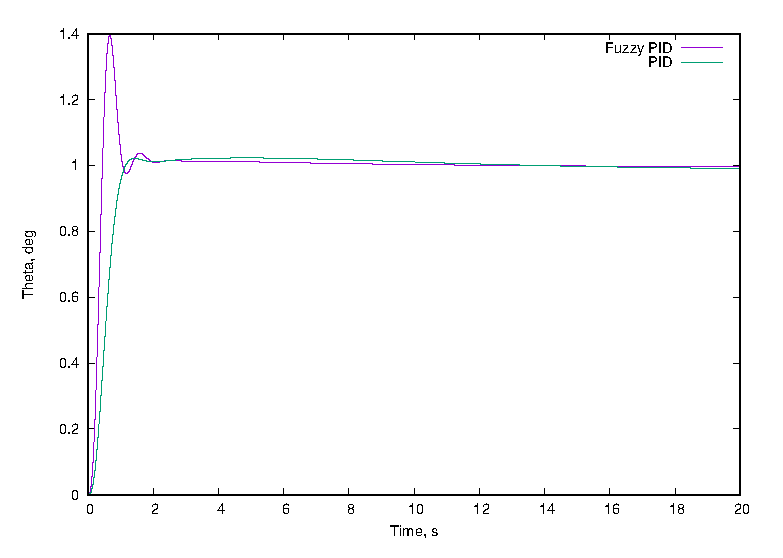
\includegraphics[width=0.49\textwidth]{results/f4_approach}}
        \subfigure[\label{f:f4_degraded}Degraded aerodynamic derivative approach condition]
            {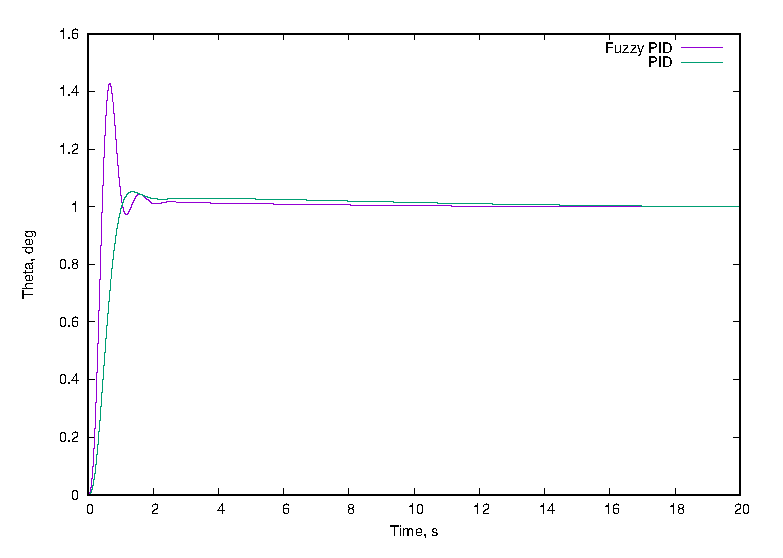
\includegraphics[width=0.49\textwidth]{results/f4_deg}}
        \subfigure[\label{f:f4_subsonic}Subsonic cruise condition]
            {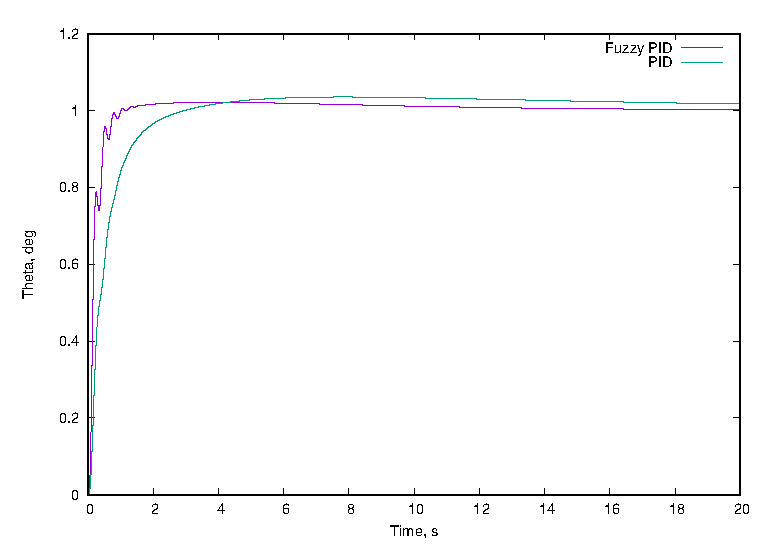
\includegraphics[width=0.49\textwidth]{results/f4_sub}}
        \subfigure[\label{f:f4_supersonic}Supersonic cruise condition]
            {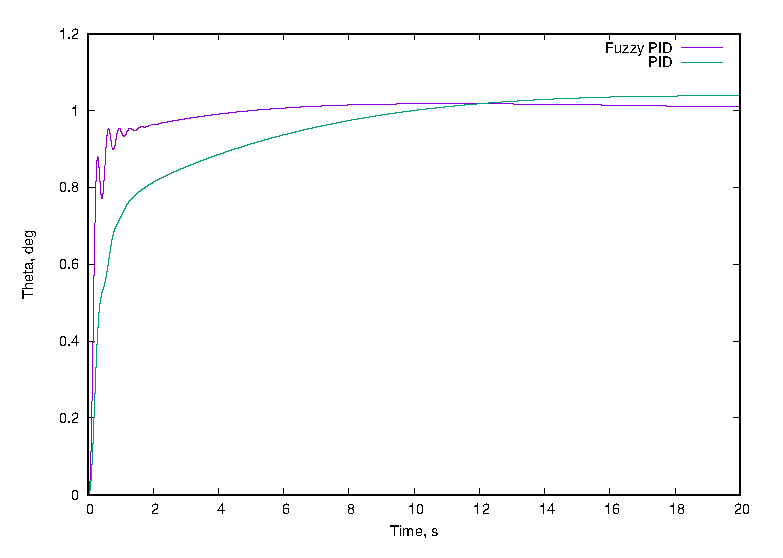
\includegraphics[width=0.49\textwidth]{results/f4_sup}}
    \end{subfigmatrix} \caption{Step response for various flight conditions. Note the increased overshoot for
                                nominal conditions from the Fuzzy-PID controller.}\label{f:f4}
\end{figure}

\begin{figure}[ht]
    \centering 
    \begin{subfigmatrix}{2}
        \subfigure[\label{f:f4_nominal_nos}Nominal approach condition]
            {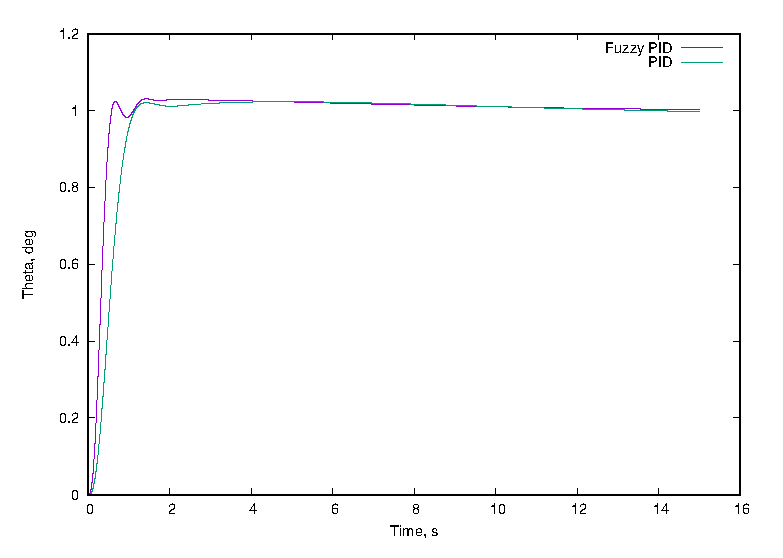
\includegraphics[width=0.49\textwidth]{results/test/f4_approach}}
        \subfigure[\label{f:f4_degraded_nos}Degraded aerodynamic derivative approach condition]
            {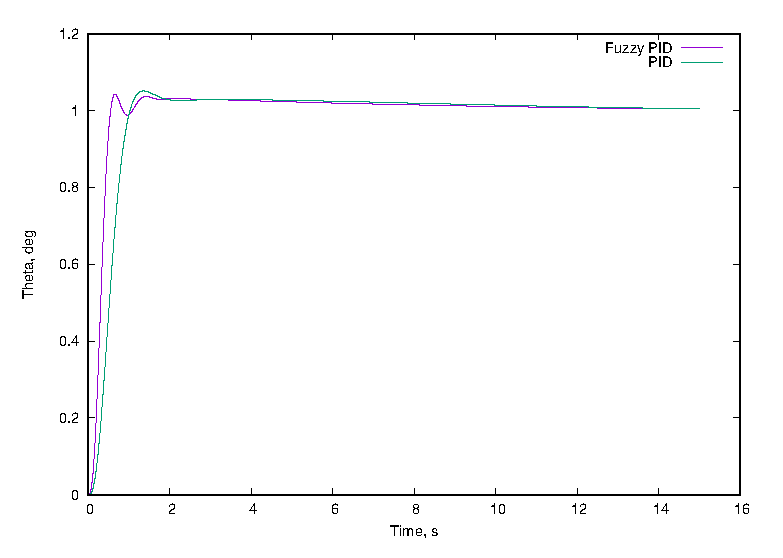
\includegraphics[width=0.49\textwidth]{results/test/f4_deg}}
        \subfigure[\label{f:f4_subsonic_nos}Subsonic cruise condition]
            {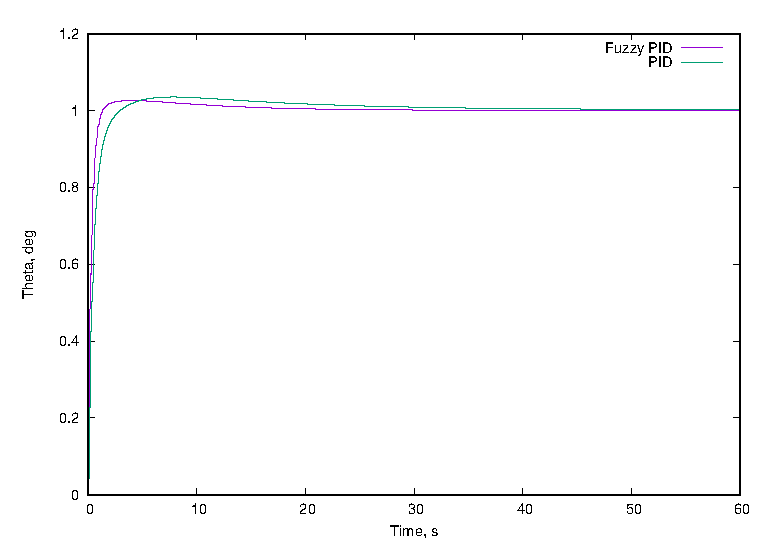
\includegraphics[width=0.49\textwidth]{results/test/f4_sub}}
        \subfigure[\label{f:f4_supersonic_nos}Supersonic cruise condition]
            {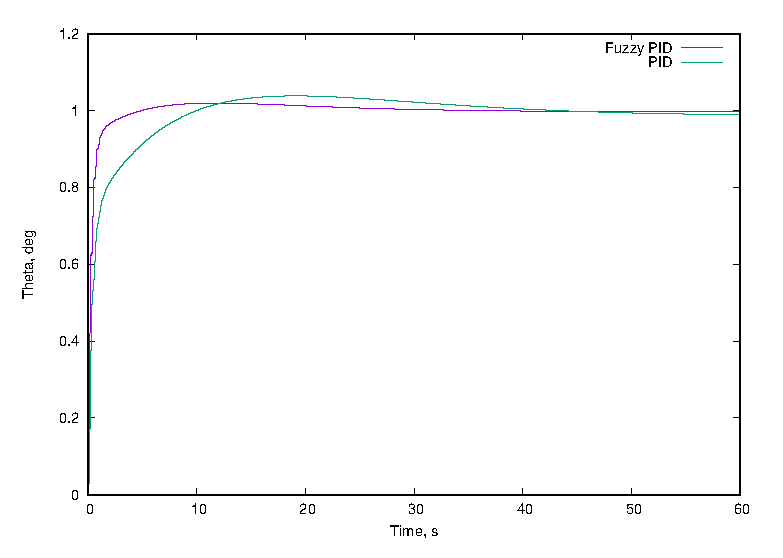
\includegraphics[width=0.49\textwidth]{results/test/f4_sup}}
    \end{subfigmatrix}
    \caption{Step response for various flight conditions using the controller created with modified cost
        function. Note the significantly decreased overshoot for nominal and degraded flight
    conditions.}\label{f:f4_nos}
\end{figure}

\begin{sidewaystable}
    \centering
    \caption{Comparison table of current results with those of Bossert and Cohen}\label{t:f4}
    \begin{tabular}{|c|c|c|c|c|c|}\hline
        Case
            & $T_s$ (s) & $T_r$ (s) & $T_p$ (s) & $M_p$ (deg) & FV (deg) \\\hline
        Root Locus F4 Approach (Design Condition)
            & 23.6      & 1.09      & 3.14      & 1.09        & 0.62 \\\hline
        PID F4 Approach (Design Condition)
            & 7.08      & 1.27      & 4.98      & 1.023       & 1.00 \\\hline
        Fuzzy F4 Approach (Design Condition)
            & 1.65      & 1.68      & 1.74      & 1.013       & 1.00 \\\hline
        \textbf{Fuzzy PID Approach (Design Condition)}
            & 1.86 & 0.26 & 0.66 & 1.396 & 1.00\\\hline

        Root Locus 50\% Red in $C_{m\alpha}$ and $C_{mq}$
            & 25.8      & 1.16      & 3.57      & 1.42        & 0.77 \\\hline
        PID 50\% Red in $C_{m\alpha}$ and $C_{mq}$
            & 8.0       & 1.03      & 1.35      & 1.045       & 1.01 \\\hline
        Fuzzy 50\% Red in $C_{m\alpha}$ and $C_{mq}$
            & 1.66      & 1.69      & 1.75      & 1.014       & 1.00 \\\hline
        \textbf{Fuzzy PID 50\% Red in $C_{m\alpha}$ and $C_{mq}$}
            & 1.87 & 0.25 & 0.66 & 1.428 & 1.00\\\hline

    \end{tabular}
    \bigskip
    \bigskip
    \bigskip
    \caption{Resulting FIS response from GA with modified cost function}\label{t:f4_nos}
    \begin{tabular}{|c|c|c|c|c|c|}\hline
        Case & $T_s$ (s) & $T_r$ (s) & $T_p$ (s) & $M_p$ (deg) & FV (deg) \\\hline
        Fuzzy PID Approach (Design Condition) & 4.96 & 0.34 & 1.43 & 1.031 & 1.00\\\hline

        Fuzzy PID 50\% Red in $C_{m\alpha}$ and $C_{mq}$ & 4.47 & 0.33 & 0.66 & 1.043 & 1.00\\\hline

    \end{tabular}
\end{sidewaystable}

\begin{table}[ht]
    \centering
    \caption{Comparison of response times for subsonic and supersonic cruise conditions for original and
             modified cost function. Modifying the cost function showed no improvements for this set of
             conditions, rather only proved to slow the response time with no gain in overshoot.}%
             \label{t:subsup}
    \begin{tabular}{|c|c|c|c|c|c|}\hline
        Case & $T_s$ (s) & $T_r$ (s) & $T_p$ (s) &
        $M_p$ (deg) & FV (deg) \\\hline Subsonic Cruise (Orig. Cost) & 0.93 & 0.38 & 3.91 & 1.022 & 1.00\\\hline
 Supersonic Cruise (Orig.
        Cost) & 3.84 & 0.73 & 11.10 & 1.018 & 1.01\\\hline
 Subsonic Cruise (Mod. Cost) & 7.97 & 0.59 & 4.09 & 1.026 & 1.00\\\hline
 Supersonic Cruise (Mod.
        Cost) & 15.53 & 0.73 & 11.74 & 1.020 & 1.00\\\hline

    \end{tabular}
\end{table}


As can be seen from \crefrange{t:f4}{t:f4_nos}, the settling time of the step response is significantly
slower when training a controller using the new cost function. However, the overall response is arguably better due
to the reduced overshoot. Additionally, though not nearly as good for the nominal and degraded flight conditions as was Bossert and
Cohen's solution, the response for the subsonic and supersonic cruise conditions show arguably better
performance (see \cref{t:subsup}).

\section{Conclusion}
In order to demonstrate the flexibility of a fuzzy PID controller, a controller was designed to meet the
demands of the approach condition of an F4 fighter. It was shown that this controller exhibited good behavior
across a wider domain than that in which it was trained. This demonstrates that an adaptive fuzzy PID
controller can be an effective approach to problems with a wide variety of scenarios.

Future will work include assessing the response of the aircraft to fuzzy PID control according to the C*
criterion, Gibson's drop back criterion, and other flying qualities standards\cite{standard1990flying}. This will provide a richer
assessment of the controller's performance.


%\chapter{Fuzzy Landing}\label{c:landing}
\chapter{Fuzzy Landing}\label{c:landing}
\section{Introduction}
With the ever-increasing proliferation of small unmanned air vehicles (sUAVs) and their use in commercial and
emergency response applications, there is a growing need for intelligent, reliable control methodologies to
safely manage their navigation, especially in possibly congested areas such as disaster areas or urban
centers. Commercial delivery companies are moving towards an automated model with reduced human operator
intervention to increase the efficiency of their deliveries. One such model consists of a vehicle-based sUAV
which departs from the delivery vehicle to make a delivery to a remote residence. Upon completing the
delivery, the sUAV returns to the vehicle and docks to receive additional packages. Considering the small
target size of a landing platform affixed to the potentially moving vehicle, and the highly dynamic conditions
in which deliveries may be accomplished, the control effort must be accurate and robust in the face of
disturbances.

Fuzzy control is able to accommodate nonlinearities in the dynamic system such as are found in the situation
of an air vehicle to ground transport rendezvous\cite{Ionita_2005}. Current approaches for
developing trajectory paths have focused on time-optimality\cite{Adams_2012}\cite{Hehn_2012} and not
necessarily on lightweight, on-board controllers. In contrast, this work optimizes for reduced control
effort, as well as computational simplicity and efficiency. Accuracy is paramount, as the target platform is
nearly equally-sized to the sUAV.

\section{System Architecture}
The research setup consists of a quadrotor aircraft of size \SI{450}{\mm} on the diagonal and a mobile rover
robot with a \SI{255}{mm} radius landing platform affixed to it (as shown in \cref{f:lezl-olli}). The
quadrotor is controlled by a Pixhawk flight controller which uses the PX4 flight control firmware. This flight
controller allows for an on-board computer to take over control of the aircraft via a serial wire connection.
A small Linux-based computer is placed on the quadrotor which sends velocity setpoints to the flight
controller. All control logic is written in Python using a collection of softwares called Robot Operating
System (ROS). ROS allows for easy integration of sensors and control actuation due to a distributed
computation framework. As a highly event-driven, publish-subscribe model, ROS maintains an accurate,
up-to-date view of internal states which are then exposed to any connected nodes.

An assumption is made that GPS (or some other global positioning) data is available for the simulation;
however, this positioning has a margin of error which is far too large to be used exclusively for precision
landing. For this reason, an on-board camera is utilized to detect and locate the target. Using the
characteristics of the camera focal length and distortion coefficients, an accurate positional error can be
obtained for the feedback control loop. 

\begin{figure}[ht!]
    \centering
    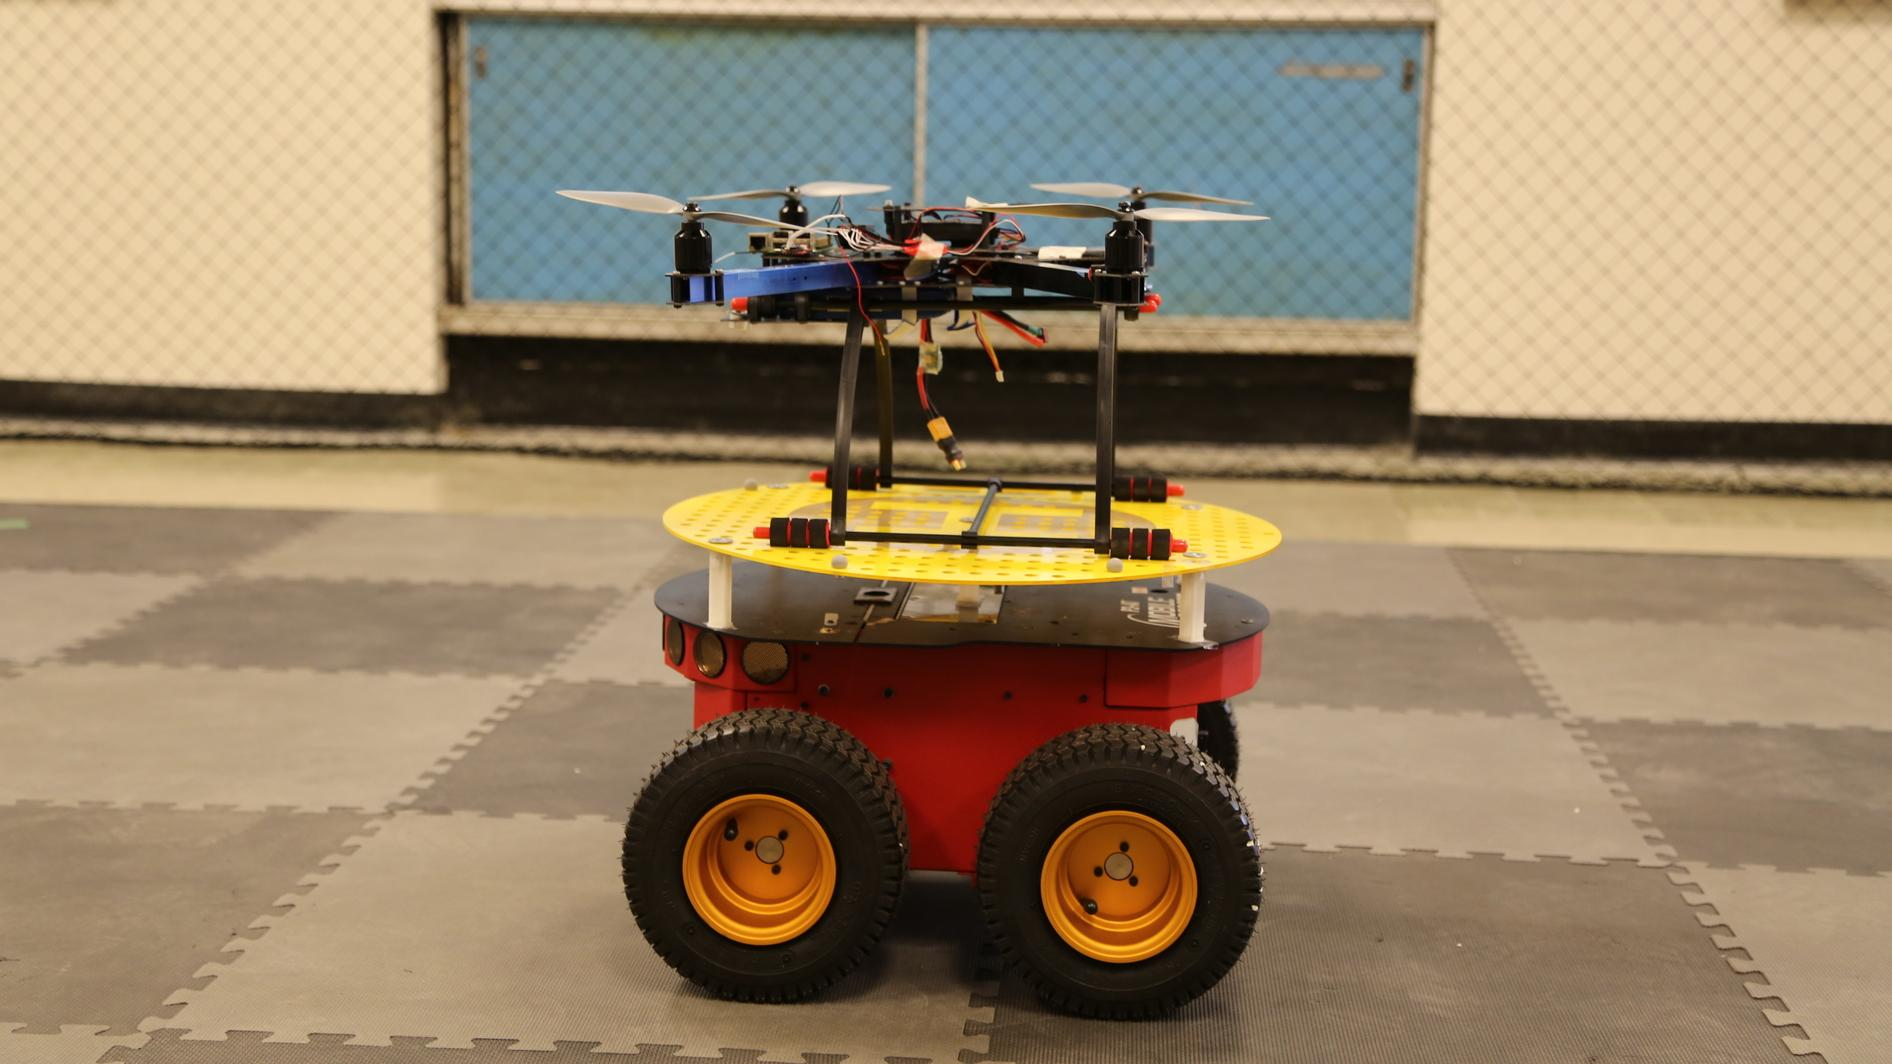
\includegraphics[width=0.6\textwidth]{images/irols.jpg}
    \caption{The test sUAV with the mobile target platform.}\label{f:lezl-olli}
\end{figure}

\subsection{Simulation}
Gazebo is a 3D simulation software which uses open source dynamics engines Bullet, Dart, and ODE to model its
components. While Gazebo has very high fidelity simulation capabilities for robots (its initial purpose), the
complexities of aerodynamics in general, and multicopter physics in particular, can only be modeled with many
simplifications. Even with the simplified dynamics, the simulation environment that Gazebo provides is very
useful for high-level controller development. Gazebo allows for the simulation of many sensor types and nicely
integrates with ROS and the PX4 flight controller firmware. The simulation
provides a real time interface for tuning the controller with visual feedback. This is the process which was
used to tune the fuzzy controller.

The most important aspect of sensing for the system is the image sensor. A camera sensor is simulated from the
underside of the quadrotor to test the efficacy and efficiency of the computer vision algorithms. Care was
taken to accurately represent the field of view and pixel noise of the physical camera sensor to be used.


\subsection{Onboard Software} ROS is an open source framework developed specifically to ease the development
of software for robotics and robotics control\cite{quigley2009ros}. Using ROS, it becomes a simple task to
distribute computational loads across a computational graph of separate nodes. Additionally, ROS has a rich
library of packages which are useful for both low-level processing of sensor information or managing hardware
interfaces, and also high-level behavioral control or localization schemes. This project use a number of such
packages to perform tasks in the areas of visual odometry\cite{olson2011tags}, kalman filtering
\cite{MooreStouchKeneralizedEkf2014}, and flight control\cite{rotors:2016,meier2015px4}. ROS allows for a
system designer to aggregate any number of processing units, called nodes, into a  complex computational graph.
An example of the graph structure created to complete this work is shown in \cref{f:rosgraph} and provides a
visualization of this complex structure. Each node in the graph represents a unit of computation which
consumes information from another node in the graph. Each edge in the graph represents a direct message
passing pipeline through which information is transmitted. Each node runs continuously and in parallel,
facilitating the creation of reactive, concurrent systems.

\begin{figure}[H]
    \centering
    \includedot[scale=0.29]{tikz/rosgraph_notf_cluster}
    \caption{Computational node graph for a typical landing simulation. Note that this graph may change over
    time as node may be dynamically started and stopped. Likewise, message passing pipelines may be opened or
    closed at any time.}\label{f:rosgraph}
\end{figure}

The nodes can be broadly categorized into three groups: Sensing nodes, Action states, and Control loop nodes.
The Sensing nodes consume image sensor output and pre-process it for Kalman filtering.
The Action states each represent a state in the state machine. These represent basic actions which the vehicle
can perform and can be aggregated to construct more complex behavior. The nodes in the Control loop represent
the plant (\verb|/mavros|), the sensor (\verb|/ekf_odom|), and the compensator (\verb|/flc_action|). In this
way, it becomes easy to visualize the canonical form of a feedback control loop. As can be seen in
\cref{f:rosgraph}, the structure allows a roboticist to build and manage highly complex systems in a
maintainable way.

\begin{figure}[H]
    \centering
    \includedot[scale=0.39]{tikz/smach}
    \caption{State machine of robotic lander}\label{f:smach}
\end{figure}

Control of the quadcopter is handled in discrete stages based on vehicle state. It is assumed that the vehicle
will have a rough estimate of the target location given to it so that it can travel to the appropriate region
and find the target in the field of view of the camera sensor. Vehicle motion from arming until target
location is handled by sending waypoints to the flight controller. Once the target is located in the image,
the vehicle gives control over to a set of FISs. The controller is described in more detail in
\cref{s:landing:controller}. The vehicle behavior over an entire mission is handled using a state
machine\cite{bohren2010smach}. Using a state machine allows the control to be handled in well-defined domains
and ensures that transitions between states are handled smoothly. The states comprising a full mission from
takeoff to landing are shown in \cref{f:smach}. A link to the video showing a full landing mission can be
found in the references section\cite{yt_stat}. An annotated image of the simulation at each state can be found
in \cref{app:smach} (example in \cref{f:sim_static_shot}).

\begin{figure}
    \centering
    \includegraphics[width=0.6\textwidth]{images/static_captures/static-15h39m54s115}
    \caption{Image of the simulation and live state diagram while vehicle is approaching the
    platform.}\label{f:sim_static_shot}
\end{figure}

The state of the vehicle is managed by fusing together the positional estimate from the camera sensor and the
AprilTag estimate (see \cref{s:landing:cv}), as well as orientation information from the onboard IMU using an
extended kalman filter (EKF). This estimate is only valid when the vehicle has a visual track on the target
platform; otherwise, it is assumed that the vehicle is still in transit from its launch location, or it has
landed. 

As can be seen in \cref{f:smach}, a mission starts in the ``ARM'' by arming the vehicle and immediately
sending it a waypoint which is near the target's location. Once the vehicle has received the waypoint, it
enters the ``TRACK'' state and is en route to the target location. While in this state, it monitors the
quality of its visual estimation of the target location by evaluating the norm of the covariance matrix 
computed by the EKF. Only when the covariance is sufficiently small does the vehicle transition to the next
state.

The transition to the ``APPROACH\_LAND'' state signals the transfer of control from the flight controller's
waypoint manager to the FISs. The "APPROACH\_LAND" state is simply a composition of two substates, "APPROACH"
and "LAND". During the "APPROACH" substate, the EKF is still running, sending estimates to the fuzzy logic
controller. The fuzzy logic controller is sending velocity setpoints to the onboard flight controller, thus
closing the feedback loop. The desired outcome of this state is to get the vehicle in a position above
the platform such that we can initiate the landing sequence. When the vehicle meets a proximity threshold,
it transitions to the ``LAND'' substate and puts down onto the landing pad. The details of the simulation,
control, vision estimation, and development process are discussed at length in the following sections.

\subsection{Computer Vision}\label{s:landing:cv}
Image processing is handled by a node in the ROS computation graph that is constantly processing image outputs
from the onboard camera. Once it senses the platform, it then publishes
a state estimation to the rest of the nodes in the ROS graph. Much emphasis is put on the sensing algorithms to be computationally efficient to decrease the load on the
on-board computer. For this purpose, only a small number of image processes are required to detect and locate
the target. As a first pass, the image is brought into the Hue-Saturation-Value (HSV) color space. This has
been shown to be a robust space in which to perform color detection and segmentation in uncontrolled and
unpredictable lighting conditions\cite{zhao2002robust}. A simple thresholding is performed on the image to
isolate a sufficiently wide band of yellows to match the color of the target and dilate this to a binary blob.
From this binary image, the image moments are calculated by
\begin{figure}[ht!]
    \centering
    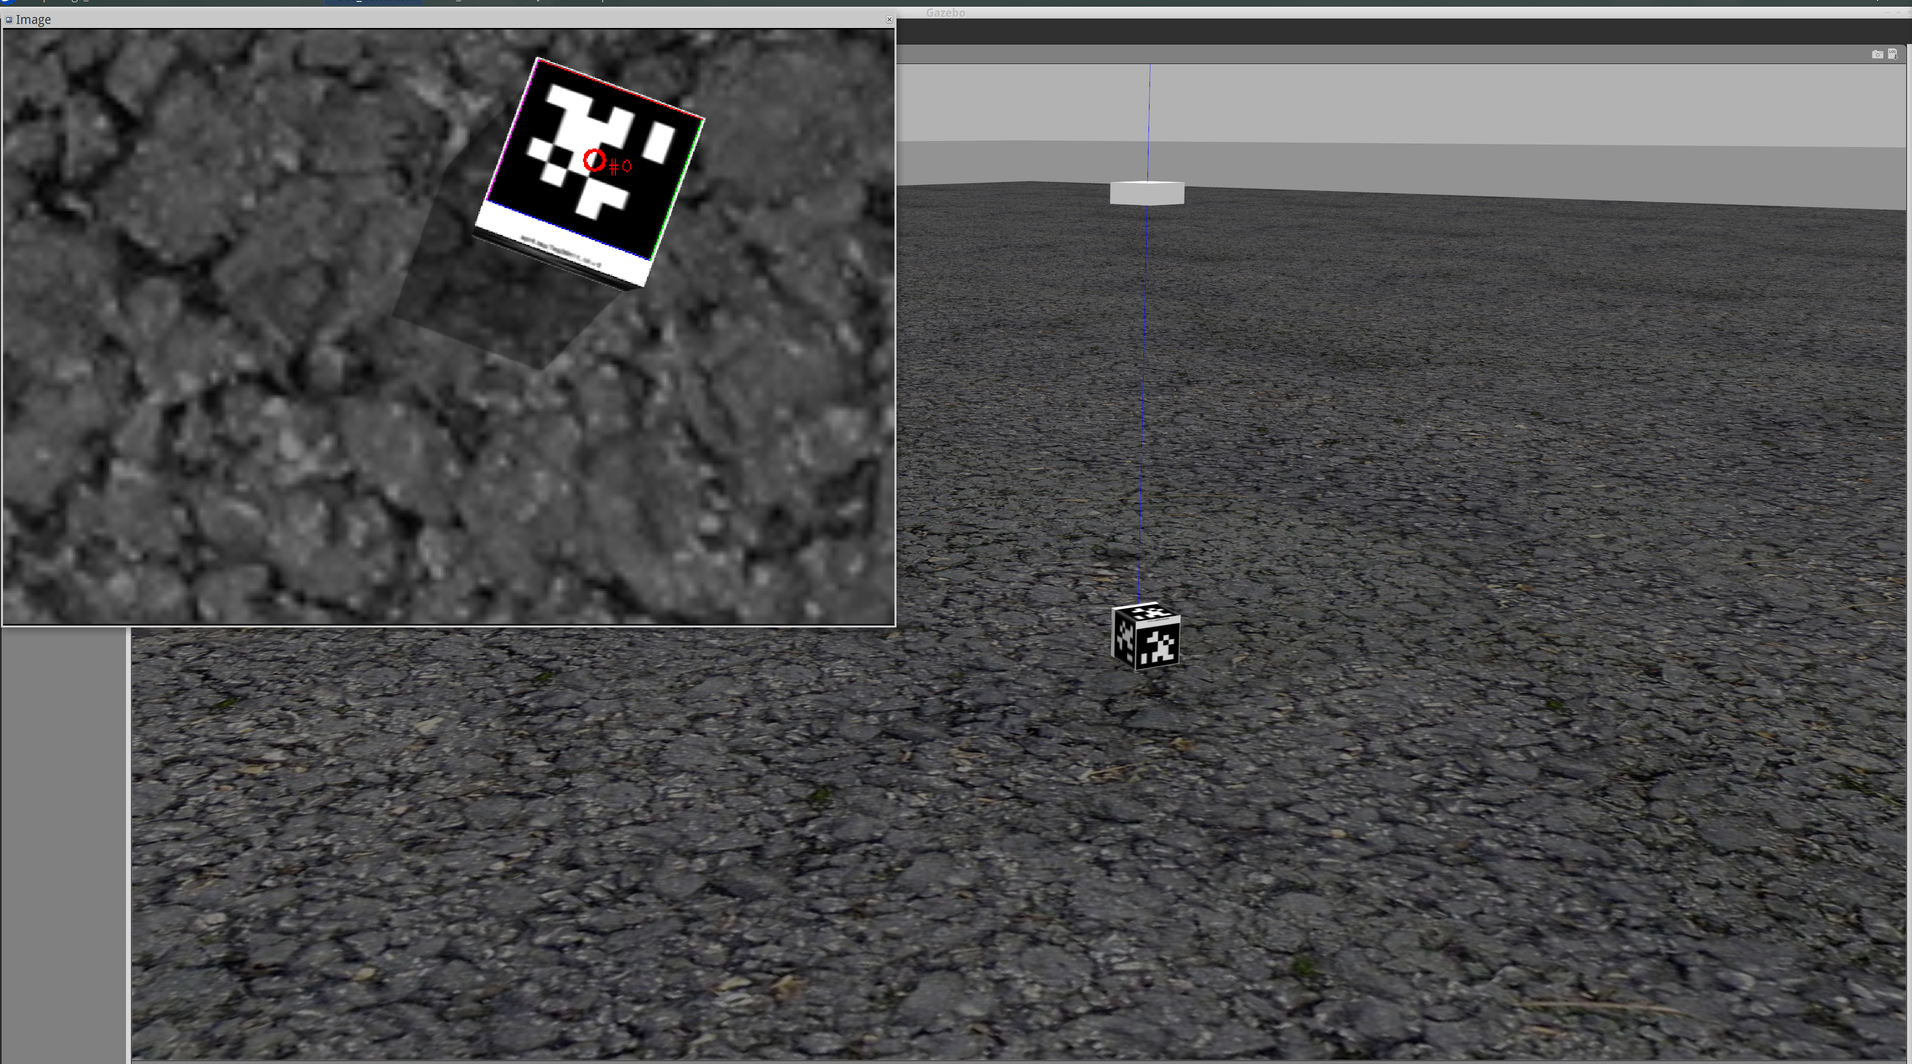
\includegraphics[width=0.8\textwidth]{images/rs_working_apriltags_crop.png}
    \caption{Simulated image sensor detection of AprilTag marker.}\label{f:apriltag}
\end{figure}

\begin{equation}\label{e:im_moments} 
    m_{ij}=\sum_{x,y}x^iy^jI_{xy}
\end{equation}
\nomenclature[]{$m_{ij}$}{Raw image moment}
\nomenclature[]{$I_{xy}$}{Pixel intensity value}
where $I_{xy}$ is the pixel intensity value for each pixel $(x,y)$ (equal to 1 for this binary blob) and $i,j
= 0,1,2$. From this it can be seen that $m_{00}$ describes the area and $\frac{m_{10}}{m_{00}}$ and
$\frac{m_{01}}{m_{00}}$ describe the centroids $\overline{x}_p$ and $\overline{y}_p$ in terms of
pixels\cite{hu1962visual}. The blob is assumed to be circular and hence a diameter is extracted from the pixel
area. Using the focal length of the sensor, these image points are then projected onto the ground plane using
the known diameter of the landing pad and a vertical offset estimate is obtained as is shown in
\cref{e:dist_est}.
\begin{equation}\label{e:dist_est}
    d_z=\frac{d\cdot f}{m\cdot d_p}
\end{equation}
where $f$ is the focal length of the camera in units of length, $d$ is the known diameter of the landing pad,
$d_p$ is the estimated diameter in pixels, and $m$ represents a scaling factor in units of \si{\px\per\mm}
(unity in the simulation).
\nomenclature[]{$f$}{Focal length of image sensor}
\nomenclature[]{$m$}{Pixel scaling factor}
Assuming that the image plane and the ground plane are parallel, the center of the image can be assumed to
point directly below the vehicle and the horizontal offsets to the landing pad can then be calculated as
\begin{align}\label{e:horiz_est}
    d_x &= d_z\cdot\frac{m\overline{x}_p}{f}\\
    d_y &= d_z\cdot\frac{m\overline{y}_p}{f}\label{e:horiz_est-y}
\end{align}
\nomenclature[]{$d_x$}{Horizontal offset error from vehicle to target in the body-fixed $x$-axis}
\nomenclature[]{$d_y$}{Horizontal offset error from vehicle to target in the body-fixed $y$-axis}
\nomenclature[]{$d_z$}{Vertical offset error from vehicle to the target}

Unless the camera is mounted to a perfect gimbal, the image plane cannot be assumed to be parallel to the
ground plane, thus invalidating \crefrange{e:horiz_est}{e:horiz_est-y}. To overcome this, the rotation
sequence needed to transform the image into body-relative coordinates is found and applied to the image data.
The camera is assumed to be rigidly affixed to the body of the vehicle, thus this is a simple static
transformation. Then, the vehicle body frame is related to the inertial frame by another rotation. The landing
pad is assumed to be on level ground and the distance between the vehicle and pad is estimated from
\cref{e:dist_est}. Note that although there will be image skew when the vehicle is under some rotation, the error in estimated distance this introduces is small compared to the actual distance of the vehicle from
the target. As the vehicle approaches the target, the estimate improves in quality due to a crisper image,
level flight, and the addition of AprilTag estimation.

In order to account for vehicle attitude, a rotation sequence is applied to the projected target location.
Let $R\left(\phi, \theta, \psi\right)$ be the rotation matrix defined as
\begin{equation}
    R(\phi,\theta,\psi) = 
    \begin{bmatrix}
            c_{\theta}c_{\psi}                           & -c_{\theta}s_{\phi}                           & s_{\theta}\\
            c_{\phi}s_{\psi} + c_{\psi}s_{\phi}s_{\theta} & c_{\phi}c_{\psi} - c_{\psi}s_{\phi}s_{\theta} & -c_{\theta}s_{\phi}\\
            s_{\phi}s_{\psi} -c_{\phi}c_{\psi}s_{\theta} & c_{\psi}s_{\phi} + c_{\phi}s_{\theta}s_{\psi} & c_{\phi}c_{\theta}
    \end{bmatrix}
\end{equation}
where $\phi$, $\theta$, and $\psi$ are vehicle roll, pitch and yaw respectively. $c_{\alpha}$ and $s_{\alpha}$
represent $\cos{\alpha}$ and $\sin{\alpha}$ respectively. Let $R_x^y$ represent the rotation from frame $x$ to
$y$, then $R_x^yR_y^z$ is the rotation from frame $x$ to frame $z$ with respect to the stationary frame $x$.
Now assuming the vehicle can estimate its orientation from the onboard inertial measurement unit, the
following rotation matrices can be defined.
\begin{align}
    R_{cam}^{body}   & = R(\pi, 0, 0)\label{e:rot_cam_bod}\\
    R_{body}^{inert} & = R(\phi, \theta, \psi)\label{e:rot_body_inert}
\end{align}
where $R_{x}^{y}$ represents the rotation from frame $x$ to frame $y$. These rotations are then prefixed to the
projected point found  in \crefrange{e:dist_est}{e:horiz_est-y} to find the point in world units with respect
to the vehicle.
\begin{align}\label{e:rotate}
    P_i = \begin{pmatrix}d_x\\d_y\\d_z\end{pmatrix}\\
    P_r = R_{body}^{inert}R_{cam}^{body}P_i
\end{align}
where $P_i$ is the projected point of the target in the plane parallel to the image plane, and $P_r$ is the
rotated point of the target with respect to the vehicle.

As the vehicle approaches the landing pad, the image field of view is overtaken by the landing pad itself and
the former segmentation no longer becomes effective. For this purpose, an AprilTag\cite{olson2011tags} (see
\cref{f:apriltag}) is placed on the center of the target. In \cref{f:landing_ims}, a landing approach is
illustrated from the viewpoint of the image sensor. This figure shows three different stages of the image
processing pipeline: raw image capture ( \crefrange{f:colora}{f:colorb}), AprilTag detection
(\crefrange{f:aprila}{f:aprilb}), and platform detection (\crefrange{f:cva}{f:cvb}). Individual estimates from
both the AprilTag detection and platform detection are then fused using an EKF (\cref{s:ekf}). 

\begin{figure}
    \begin{subfigmatrix}{4}% number of columns
        \subfigure[\label{f:colora}]{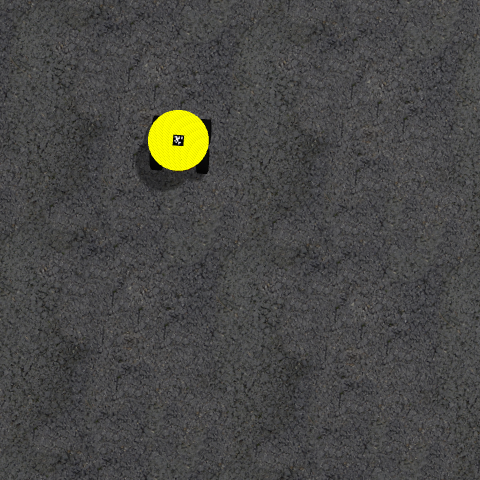
\includegraphics[width=0.2\textwidth]{images/image1_18469000.png}}
        \subfigure[]{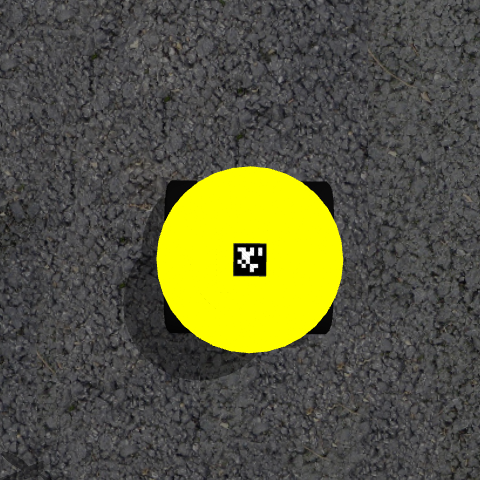
\includegraphics[width=0.2\textwidth]{images/image1_30863000.png}}
        \subfigure[]{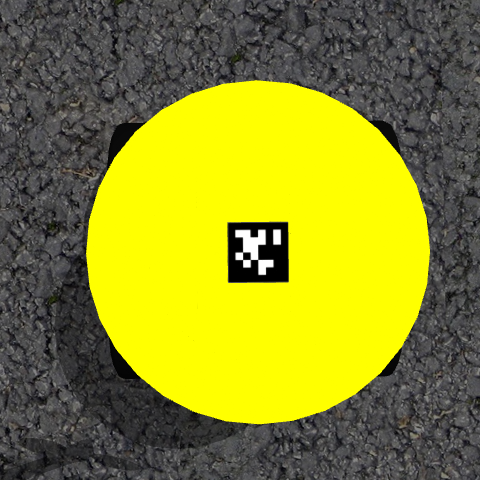
\includegraphics[width=0.2\textwidth]{images/image1_36074000.png}}
        \subfigure[\label{f:colorb}]{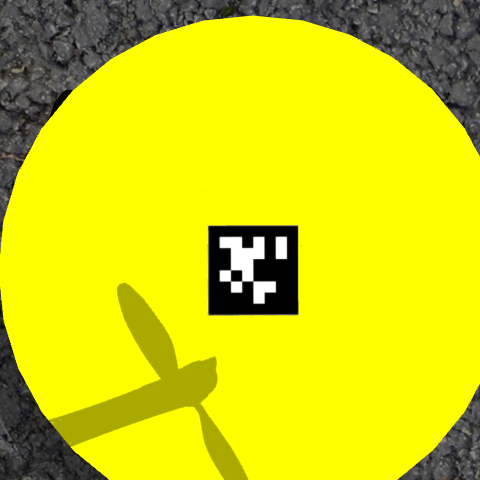
\includegraphics[width=0.2\textwidth]{images/image1_38233000.png}}
        \subfigure[\label{f:aprila}]{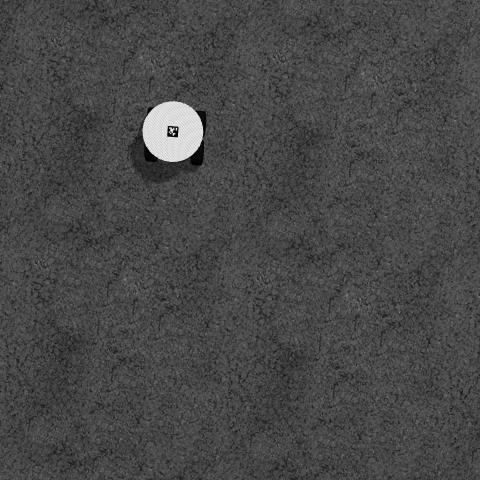
\includegraphics[width=0.2\textwidth]{images/image2_18469000.png}}
        \subfigure[]{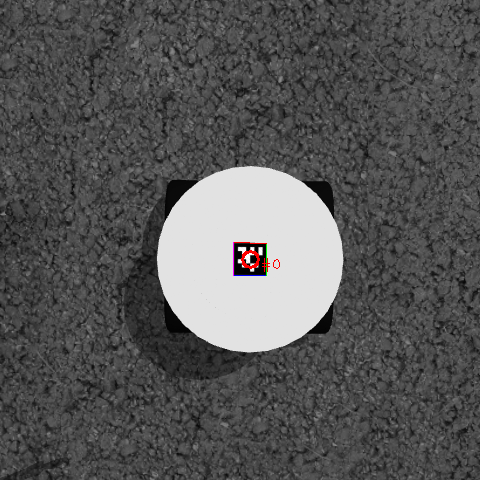
\includegraphics[width=0.2\textwidth]{images/image2_30863000.png}}
        \subfigure[]{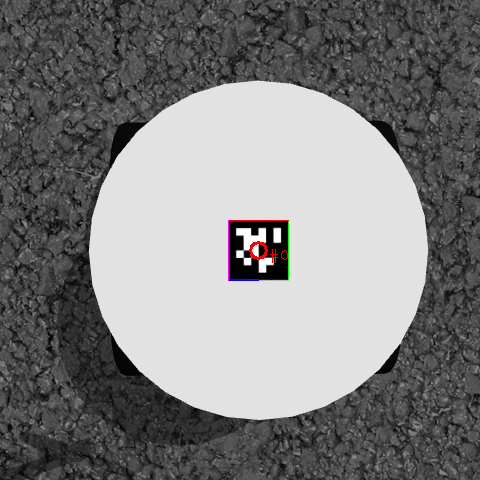
\includegraphics[width=0.2\textwidth]{images/image2_36074000.png}}
        \subfigure[\label{f:aprilb}]{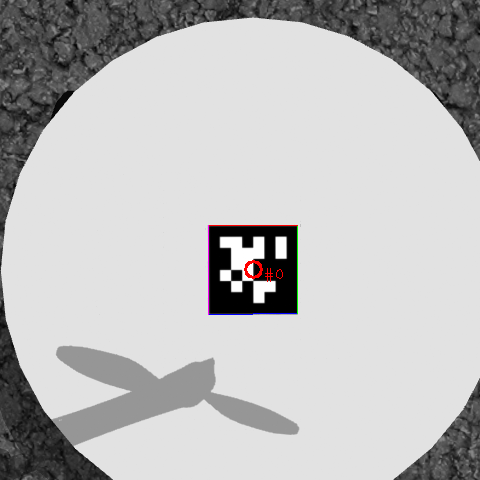
\includegraphics[width=0.2\textwidth]{images/image2_38233000.png}}
        \subfigure[\label{f:cva}]{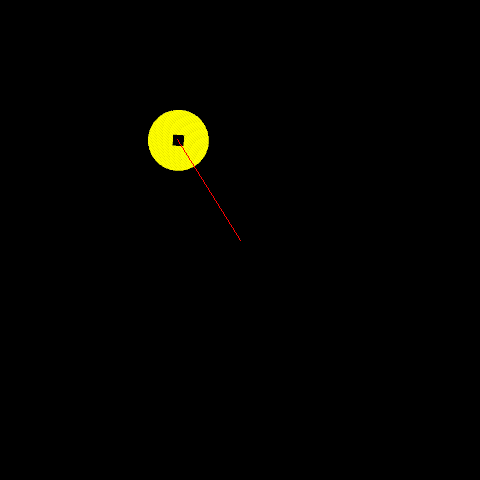
\includegraphics[width=0.2\textwidth]{images/image1_18469000_proc.png}}
        \subfigure[]{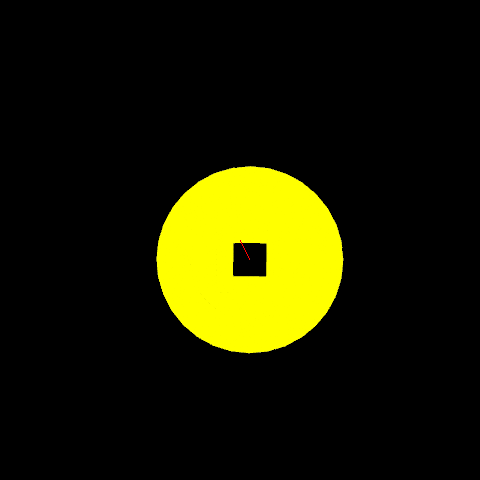
\includegraphics[width=0.2\textwidth]{images/image1_30863000_proc.png}}
        \subfigure[]{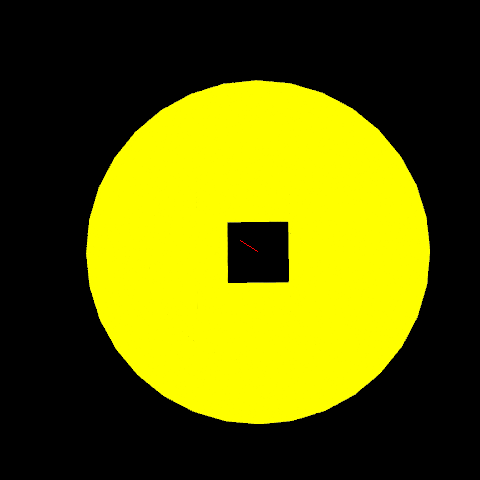
\includegraphics[width=0.2\textwidth]{images/image1_36074000_proc.png}}
        \subfigure[\label{f:cvb}]{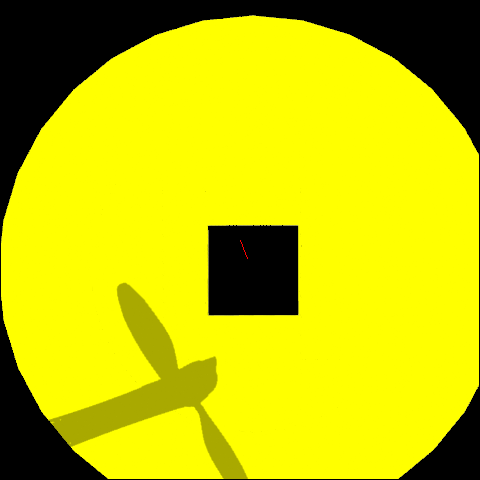
\includegraphics[width=0.2\textwidth]{images/image1_38233000_proc.png}}
    \end{subfigmatrix}
    \caption{A time series of images taken during the landing maneuver.}
    \label{f:landing_ims}
\end{figure}

\section{Controller}\label{s:landing:controller}
Control is actuated on the vehicle by providing velocity setpoints to the flight controller, $v_x$, $v_y$,
$v_z$, and yaw rate, $\dot{\psi}$. Ideally either linear acceleration setpoints or forces would be the control
output, but limitations in the flight controller make this impossible at this time. Setting velocities allows
the controller to cope with step changes to position offset well, but have difficulties tracking ramps. The
yaw angle, $\psi$ of the vehicle at landing is irrelevant for this project, but the controller is able to
control that axis regardless.

\subsection{PID Controller}
A PID controller was created which uses error estimates and sends velocity setpoints to the flight controller.
Due to the lack of a mathematical model of the system, the PID gains were found by iterating the simulation
with various position setpoints and dynamically adjusting the gains while observing the response visually.
This closely mimics the method by which PID gains are attained in the tuning of an actual quadrotor by flying
a series of test flights and adjusting gain values by feel. In this way, a reasonable response and landing
sequence was achieved for first a static target and then repeated for a dynamic target moving with constant
velocity. The results are presented in \crefrange{f:pid_stat}{f:pid_dyn} in which the normed horizontal offset
from target is shown in conjunction with the vertical distance to the platform. This view of the data gives an
overall sens of how the controller performs by showing how smooth the trajectory of the vehicle is as it
approaches the platform.  Viewing the charts, it is
apparent that as the vehicle approaches the target, it tends to accumulate horizontal errors and must correct
more frequently, particularly in the dynamic case. In both cases, the quadrotor managed to successfully land
on the target. In the static case, the final offset from the center of the target was less than \SI{5}{\cm}.
For the dynamic case, the error was \SI{7}{\cm} which nearly displaced it from the target surface. In both
cases, the sink rate and yaw rates were controlled by simple PD controllers. It can be seen that the controller took a significantly longer time to intercept and land
on the moving target as it repeatedly had trouble responding to the motion and would temporarily lose its
visual track. This is apparent in the large spiking errors in \cref{f:pid_dyn}.

%\begin{figure}
    %\centering
    %% GNUPLOT: LaTeX picture with Postscript
\begingroup
  \makeatletter
  \providecommand\color[2][]{%
    \GenericError{(gnuplot) \space\space\space\@spaces}{%
      Package color not loaded in conjunction with
      terminal option `colourtext'%
    }{See the gnuplot documentation for explanation.%
    }{Either use 'blacktext' in gnuplot or load the package
      color.sty in LaTeX.}%
    \renewcommand\color[2][]{}%
  }%
  \providecommand\includegraphics[2][]{%
    \GenericError{(gnuplot) \space\space\space\@spaces}{%
      Package graphicx or graphics not loaded%
    }{See the gnuplot documentation for explanation.%
    }{The gnuplot epslatex terminal needs graphicx.sty or graphics.sty.}%
    \renewcommand\includegraphics[2][]{}%
  }%
  \providecommand\rotatebox[2]{#2}%
  \@ifundefined{ifGPcolor}{%
    \newif\ifGPcolor
    \GPcolorfalse
  }{}%
  \@ifundefined{ifGPblacktext}{%
    \newif\ifGPblacktext
    \GPblacktexttrue
  }{}%
  % define a \g@addto@macro without @ in the name:
  \let\gplgaddtomacro\g@addto@macro
  % define empty templates for all commands taking text:
  \gdef\gplbacktext{}%
  \gdef\gplfronttext{}%
  \makeatother
  \ifGPblacktext
    % no textcolor at all
    \def\colorrgb#1{}%
    \def\colorgray#1{}%
  \else
    % gray or color?
    \ifGPcolor
      \def\colorrgb#1{\color[rgb]{#1}}%
      \def\colorgray#1{\color[gray]{#1}}%
      \expandafter\def\csname LTw\endcsname{\color{white}}%
      \expandafter\def\csname LTb\endcsname{\color{black}}%
      \expandafter\def\csname LTa\endcsname{\color{black}}%
      \expandafter\def\csname LT0\endcsname{\color[rgb]{1,0,0}}%
      \expandafter\def\csname LT1\endcsname{\color[rgb]{0,1,0}}%
      \expandafter\def\csname LT2\endcsname{\color[rgb]{0,0,1}}%
      \expandafter\def\csname LT3\endcsname{\color[rgb]{1,0,1}}%
      \expandafter\def\csname LT4\endcsname{\color[rgb]{0,1,1}}%
      \expandafter\def\csname LT5\endcsname{\color[rgb]{1,1,0}}%
      \expandafter\def\csname LT6\endcsname{\color[rgb]{0,0,0}}%
      \expandafter\def\csname LT7\endcsname{\color[rgb]{1,0.3,0}}%
      \expandafter\def\csname LT8\endcsname{\color[rgb]{0.5,0.5,0.5}}%
    \else
      % gray
      \def\colorrgb#1{\color{black}}%
      \def\colorgray#1{\color[gray]{#1}}%
      \expandafter\def\csname LTw\endcsname{\color{white}}%
      \expandafter\def\csname LTb\endcsname{\color{black}}%
      \expandafter\def\csname LTa\endcsname{\color{black}}%
      \expandafter\def\csname LT0\endcsname{\color{black}}%
      \expandafter\def\csname LT1\endcsname{\color{black}}%
      \expandafter\def\csname LT2\endcsname{\color{black}}%
      \expandafter\def\csname LT3\endcsname{\color{black}}%
      \expandafter\def\csname LT4\endcsname{\color{black}}%
      \expandafter\def\csname LT5\endcsname{\color{black}}%
      \expandafter\def\csname LT6\endcsname{\color{black}}%
      \expandafter\def\csname LT7\endcsname{\color{black}}%
      \expandafter\def\csname LT8\endcsname{\color{black}}%
    \fi
  \fi
    \setlength{\unitlength}{0.0500bp}%
    \ifx\gptboxheight\undefined%
      \newlength{\gptboxheight}%
      \newlength{\gptboxwidth}%
      \newsavebox{\gptboxtext}%
    \fi%
    \setlength{\fboxrule}{0.5pt}%
    \setlength{\fboxsep}{1pt}%
\begin{picture}(7200.00,5040.00)%
    \gplgaddtomacro\gplbacktext{%
      \csname LTb\endcsname%
      \put(946,704){\makebox(0,0)[r]{\strut{}$-0.5$}}%
      \csname LTb\endcsname%
      \put(946,1111){\makebox(0,0)[r]{\strut{}$0$}}%
      \csname LTb\endcsname%
      \put(946,1518){\makebox(0,0)[r]{\strut{}$0.5$}}%
      \csname LTb\endcsname%
      \put(946,1925){\makebox(0,0)[r]{\strut{}$1$}}%
      \csname LTb\endcsname%
      \put(946,2332){\makebox(0,0)[r]{\strut{}$1.5$}}%
      \csname LTb\endcsname%
      \put(946,2740){\makebox(0,0)[r]{\strut{}$2$}}%
      \csname LTb\endcsname%
      \put(946,3147){\makebox(0,0)[r]{\strut{}$2.5$}}%
      \csname LTb\endcsname%
      \put(946,3554){\makebox(0,0)[r]{\strut{}$3$}}%
      \csname LTb\endcsname%
      \put(946,3961){\makebox(0,0)[r]{\strut{}$3.5$}}%
      \csname LTb\endcsname%
      \put(946,4368){\makebox(0,0)[r]{\strut{}$4$}}%
      \csname LTb\endcsname%
      \put(946,4775){\makebox(0,0)[r]{\strut{}$4.5$}}%
      \csname LTb\endcsname%
      \put(1078,484){\makebox(0,0){\strut{}$0$}}%
      \csname LTb\endcsname%
      \put(1896,484){\makebox(0,0){\strut{}$5$}}%
      \csname LTb\endcsname%
      \put(2714,484){\makebox(0,0){\strut{}$10$}}%
      \csname LTb\endcsname%
      \put(3532,484){\makebox(0,0){\strut{}$15$}}%
      \csname LTb\endcsname%
      \put(4349,484){\makebox(0,0){\strut{}$20$}}%
      \csname LTb\endcsname%
      \put(5167,484){\makebox(0,0){\strut{}$25$}}%
      \csname LTb\endcsname%
      \put(5985,484){\makebox(0,0){\strut{}$30$}}%
      \csname LTb\endcsname%
      \put(6803,484){\makebox(0,0){\strut{}$35$}}%
    }%
    \gplgaddtomacro\gplfronttext{%
      \csname LTb\endcsname%
      \put(176,2739){\rotatebox{-270}{\makebox(0,0){\strut{}Error, m}}}%
      \put(3940,154){\makebox(0,0){\strut{}Time, s}}%
      \put(5816,4602){\makebox(0,0)[r]{\strut{}$e_{xy}$}}%
      \put(5816,4382){\makebox(0,0)[r]{\strut{}$e_z$}}%
    }%
    \gplbacktext
    \put(0,0){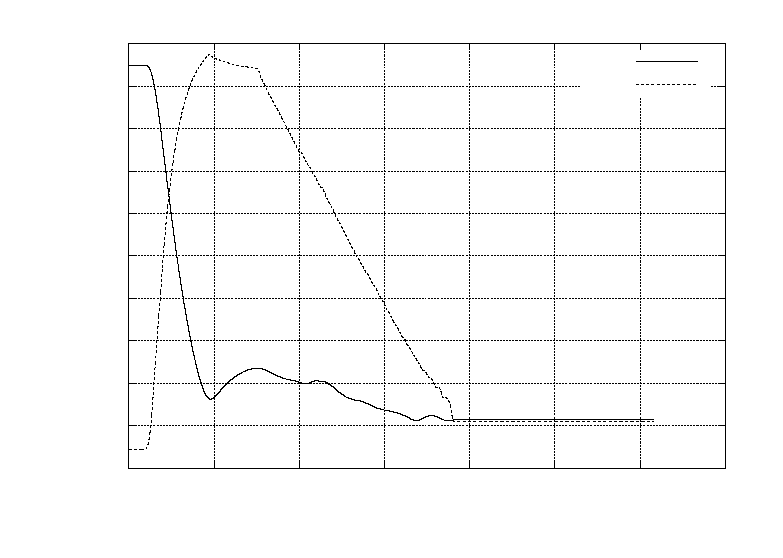
\includegraphics{static_smach_good_plot}}%
    \gplfronttext
  \end{picture}%
\endgroup

    %\caption{Fuzzy-controlled static target interception.}\label{f:fuz_stat}
%\end{figure}

%\begin{figure}
    %\centering
    %% GNUPLOT: LaTeX picture with Postscript
\begingroup
  \makeatletter
  \providecommand\color[2][]{%
    \GenericError{(gnuplot) \space\space\space\@spaces}{%
      Package color not loaded in conjunction with
      terminal option `colourtext'%
    }{See the gnuplot documentation for explanation.%
    }{Either use 'blacktext' in gnuplot or load the package
      color.sty in LaTeX.}%
    \renewcommand\color[2][]{}%
  }%
  \providecommand\includegraphics[2][]{%
    \GenericError{(gnuplot) \space\space\space\@spaces}{%
      Package graphicx or graphics not loaded%
    }{See the gnuplot documentation for explanation.%
    }{The gnuplot epslatex terminal needs graphicx.sty or graphics.sty.}%
    \renewcommand\includegraphics[2][]{}%
  }%
  \providecommand\rotatebox[2]{#2}%
  \@ifundefined{ifGPcolor}{%
    \newif\ifGPcolor
    \GPcolorfalse
  }{}%
  \@ifundefined{ifGPblacktext}{%
    \newif\ifGPblacktext
    \GPblacktexttrue
  }{}%
  % define a \g@addto@macro without @ in the name:
  \let\gplgaddtomacro\g@addto@macro
  % define empty templates for all commands taking text:
  \gdef\gplbacktext{}%
  \gdef\gplfronttext{}%
  \makeatother
  \ifGPblacktext
    % no textcolor at all
    \def\colorrgb#1{}%
    \def\colorgray#1{}%
  \else
    % gray or color?
    \ifGPcolor
      \def\colorrgb#1{\color[rgb]{#1}}%
      \def\colorgray#1{\color[gray]{#1}}%
      \expandafter\def\csname LTw\endcsname{\color{white}}%
      \expandafter\def\csname LTb\endcsname{\color{black}}%
      \expandafter\def\csname LTa\endcsname{\color{black}}%
      \expandafter\def\csname LT0\endcsname{\color[rgb]{1,0,0}}%
      \expandafter\def\csname LT1\endcsname{\color[rgb]{0,1,0}}%
      \expandafter\def\csname LT2\endcsname{\color[rgb]{0,0,1}}%
      \expandafter\def\csname LT3\endcsname{\color[rgb]{1,0,1}}%
      \expandafter\def\csname LT4\endcsname{\color[rgb]{0,1,1}}%
      \expandafter\def\csname LT5\endcsname{\color[rgb]{1,1,0}}%
      \expandafter\def\csname LT6\endcsname{\color[rgb]{0,0,0}}%
      \expandafter\def\csname LT7\endcsname{\color[rgb]{1,0.3,0}}%
      \expandafter\def\csname LT8\endcsname{\color[rgb]{0.5,0.5,0.5}}%
    \else
      % gray
      \def\colorrgb#1{\color{black}}%
      \def\colorgray#1{\color[gray]{#1}}%
      \expandafter\def\csname LTw\endcsname{\color{white}}%
      \expandafter\def\csname LTb\endcsname{\color{black}}%
      \expandafter\def\csname LTa\endcsname{\color{black}}%
      \expandafter\def\csname LT0\endcsname{\color{black}}%
      \expandafter\def\csname LT1\endcsname{\color{black}}%
      \expandafter\def\csname LT2\endcsname{\color{black}}%
      \expandafter\def\csname LT3\endcsname{\color{black}}%
      \expandafter\def\csname LT4\endcsname{\color{black}}%
      \expandafter\def\csname LT5\endcsname{\color{black}}%
      \expandafter\def\csname LT6\endcsname{\color{black}}%
      \expandafter\def\csname LT7\endcsname{\color{black}}%
      \expandafter\def\csname LT8\endcsname{\color{black}}%
    \fi
  \fi
    \setlength{\unitlength}{0.0500bp}%
    \ifx\gptboxheight\undefined%
      \newlength{\gptboxheight}%
      \newlength{\gptboxwidth}%
      \newsavebox{\gptboxtext}%
    \fi%
    \setlength{\fboxrule}{0.5pt}%
    \setlength{\fboxsep}{1pt}%
\begin{picture}(7200.00,5040.00)%
    \gplgaddtomacro\gplbacktext{%
      \csname LTb\endcsname%
      \put(682,704){\makebox(0,0)[r]{\strut{}$-1$}}%
      \csname LTb\endcsname%
      \put(682,1213){\makebox(0,0)[r]{\strut{}$0$}}%
      \csname LTb\endcsname%
      \put(682,1722){\makebox(0,0)[r]{\strut{}$1$}}%
      \csname LTb\endcsname%
      \put(682,2231){\makebox(0,0)[r]{\strut{}$2$}}%
      \csname LTb\endcsname%
      \put(682,2740){\makebox(0,0)[r]{\strut{}$3$}}%
      \csname LTb\endcsname%
      \put(682,3248){\makebox(0,0)[r]{\strut{}$4$}}%
      \csname LTb\endcsname%
      \put(682,3757){\makebox(0,0)[r]{\strut{}$5$}}%
      \csname LTb\endcsname%
      \put(682,4266){\makebox(0,0)[r]{\strut{}$6$}}%
      \csname LTb\endcsname%
      \put(682,4775){\makebox(0,0)[r]{\strut{}$7$}}%
      \csname LTb\endcsname%
      \put(814,484){\makebox(0,0){\strut{}$0$}}%
      \csname LTb\endcsname%
      \put(2012,484){\makebox(0,0){\strut{}$5$}}%
      \csname LTb\endcsname%
      \put(3210,484){\makebox(0,0){\strut{}$10$}}%
      \csname LTb\endcsname%
      \put(4407,484){\makebox(0,0){\strut{}$15$}}%
      \csname LTb\endcsname%
      \put(5605,484){\makebox(0,0){\strut{}$20$}}%
      \csname LTb\endcsname%
      \put(6803,484){\makebox(0,0){\strut{}$25$}}%
    }%
    \gplgaddtomacro\gplfronttext{%
      \csname LTb\endcsname%
      \put(176,2739){\rotatebox{-270}{\makebox(0,0){\strut{}Error, m}}}%
      \put(3808,154){\makebox(0,0){\strut{}Time, s}}%
      \put(5816,4602){\makebox(0,0)[r]{\strut{}$e_{xy}$}}%
      \put(5816,4382){\makebox(0,0)[r]{\strut{}$e_z$}}%
    }%
    \gplbacktext
    \put(0,0){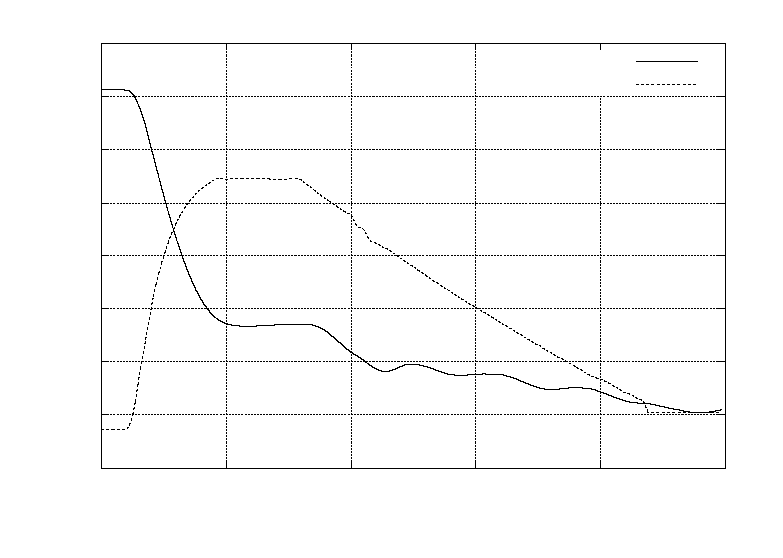
\includegraphics{moving_line_good_plot}}%
    \gplfronttext
  \end{picture}%
\endgroup

    %\caption{Fuzzy-controlled dynamic target interception.}\label{f:fuz_dyn}
%\end{figure}

\begin{figure}
    \centering
    % GNUPLOT: LaTeX picture with Postscript
\begingroup
  \makeatletter
  \providecommand\color[2][]{%
    \GenericError{(gnuplot) \space\space\space\@spaces}{%
      Package color not loaded in conjunction with
      terminal option `colourtext'%
    }{See the gnuplot documentation for explanation.%
    }{Either use 'blacktext' in gnuplot or load the package
      color.sty in LaTeX.}%
    \renewcommand\color[2][]{}%
  }%
  \providecommand\includegraphics[2][]{%
    \GenericError{(gnuplot) \space\space\space\@spaces}{%
      Package graphicx or graphics not loaded%
    }{See the gnuplot documentation for explanation.%
    }{The gnuplot epslatex terminal needs graphicx.sty or graphics.sty.}%
    \renewcommand\includegraphics[2][]{}%
  }%
  \providecommand\rotatebox[2]{#2}%
  \@ifundefined{ifGPcolor}{%
    \newif\ifGPcolor
    \GPcolorfalse
  }{}%
  \@ifundefined{ifGPblacktext}{%
    \newif\ifGPblacktext
    \GPblacktexttrue
  }{}%
  % define a \g@addto@macro without @ in the name:
  \let\gplgaddtomacro\g@addto@macro
  % define empty templates for all commands taking text:
  \gdef\gplbacktext{}%
  \gdef\gplfronttext{}%
  \makeatother
  \ifGPblacktext
    % no textcolor at all
    \def\colorrgb#1{}%
    \def\colorgray#1{}%
  \else
    % gray or color?
    \ifGPcolor
      \def\colorrgb#1{\color[rgb]{#1}}%
      \def\colorgray#1{\color[gray]{#1}}%
      \expandafter\def\csname LTw\endcsname{\color{white}}%
      \expandafter\def\csname LTb\endcsname{\color{black}}%
      \expandafter\def\csname LTa\endcsname{\color{black}}%
      \expandafter\def\csname LT0\endcsname{\color[rgb]{1,0,0}}%
      \expandafter\def\csname LT1\endcsname{\color[rgb]{0,1,0}}%
      \expandafter\def\csname LT2\endcsname{\color[rgb]{0,0,1}}%
      \expandafter\def\csname LT3\endcsname{\color[rgb]{1,0,1}}%
      \expandafter\def\csname LT4\endcsname{\color[rgb]{0,1,1}}%
      \expandafter\def\csname LT5\endcsname{\color[rgb]{1,1,0}}%
      \expandafter\def\csname LT6\endcsname{\color[rgb]{0,0,0}}%
      \expandafter\def\csname LT7\endcsname{\color[rgb]{1,0.3,0}}%
      \expandafter\def\csname LT8\endcsname{\color[rgb]{0.5,0.5,0.5}}%
    \else
      % gray
      \def\colorrgb#1{\color{black}}%
      \def\colorgray#1{\color[gray]{#1}}%
      \expandafter\def\csname LTw\endcsname{\color{white}}%
      \expandafter\def\csname LTb\endcsname{\color{black}}%
      \expandafter\def\csname LTa\endcsname{\color{black}}%
      \expandafter\def\csname LT0\endcsname{\color{black}}%
      \expandafter\def\csname LT1\endcsname{\color{black}}%
      \expandafter\def\csname LT2\endcsname{\color{black}}%
      \expandafter\def\csname LT3\endcsname{\color{black}}%
      \expandafter\def\csname LT4\endcsname{\color{black}}%
      \expandafter\def\csname LT5\endcsname{\color{black}}%
      \expandafter\def\csname LT6\endcsname{\color{black}}%
      \expandafter\def\csname LT7\endcsname{\color{black}}%
      \expandafter\def\csname LT8\endcsname{\color{black}}%
    \fi
  \fi
    \setlength{\unitlength}{0.0500bp}%
    \ifx\gptboxheight\undefined%
      \newlength{\gptboxheight}%
      \newlength{\gptboxwidth}%
      \newsavebox{\gptboxtext}%
    \fi%
    \setlength{\fboxrule}{0.5pt}%
    \setlength{\fboxsep}{1pt}%
\begin{picture}(7200.00,5040.00)%
    \gplgaddtomacro\gplbacktext{%
      \csname LTb\endcsname%
      \put(682,704){\makebox(0,0)[r]{\strut{}$-1$}}%
      \csname LTb\endcsname%
      \put(682,1213){\makebox(0,0)[r]{\strut{}$0$}}%
      \csname LTb\endcsname%
      \put(682,1722){\makebox(0,0)[r]{\strut{}$1$}}%
      \csname LTb\endcsname%
      \put(682,2231){\makebox(0,0)[r]{\strut{}$2$}}%
      \csname LTb\endcsname%
      \put(682,2740){\makebox(0,0)[r]{\strut{}$3$}}%
      \csname LTb\endcsname%
      \put(682,3248){\makebox(0,0)[r]{\strut{}$4$}}%
      \csname LTb\endcsname%
      \put(682,3757){\makebox(0,0)[r]{\strut{}$5$}}%
      \csname LTb\endcsname%
      \put(682,4266){\makebox(0,0)[r]{\strut{}$6$}}%
      \csname LTb\endcsname%
      \put(682,4775){\makebox(0,0)[r]{\strut{}$7$}}%
      \csname LTb\endcsname%
      \put(814,484){\makebox(0,0){\strut{}$15$}}%
      \csname LTb\endcsname%
      \put(1479,484){\makebox(0,0){\strut{}$20$}}%
      \csname LTb\endcsname%
      \put(2145,484){\makebox(0,0){\strut{}$25$}}%
      \csname LTb\endcsname%
      \put(2810,484){\makebox(0,0){\strut{}$30$}}%
      \csname LTb\endcsname%
      \put(3476,484){\makebox(0,0){\strut{}$35$}}%
      \csname LTb\endcsname%
      \put(4141,484){\makebox(0,0){\strut{}$40$}}%
      \csname LTb\endcsname%
      \put(4807,484){\makebox(0,0){\strut{}$45$}}%
      \csname LTb\endcsname%
      \put(5472,484){\makebox(0,0){\strut{}$50$}}%
      \csname LTb\endcsname%
      \put(6138,484){\makebox(0,0){\strut{}$55$}}%
      \csname LTb\endcsname%
      \put(6803,484){\makebox(0,0){\strut{}$60$}}%
    }%
    \gplgaddtomacro\gplfronttext{%
      \csname LTb\endcsname%
      \put(176,2739){\rotatebox{-270}{\makebox(0,0){\strut{}Error, m}}}%
      \put(3808,154){\makebox(0,0){\strut{}Time, s}}%
      \put(5816,4602){\makebox(0,0)[r]{\strut{}$e_{xy}$}}%
      \put(5816,4382){\makebox(0,0)[r]{\strut{}$e_z$}}%
    }%
    \gplbacktext
    \put(0,0){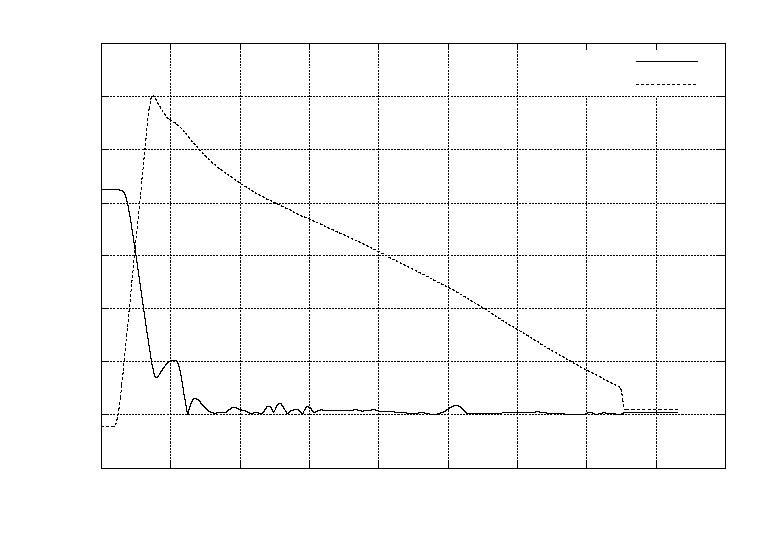
\includegraphics{pid_static}}%
    \gplfronttext
  \end{picture}%
\endgroup

    %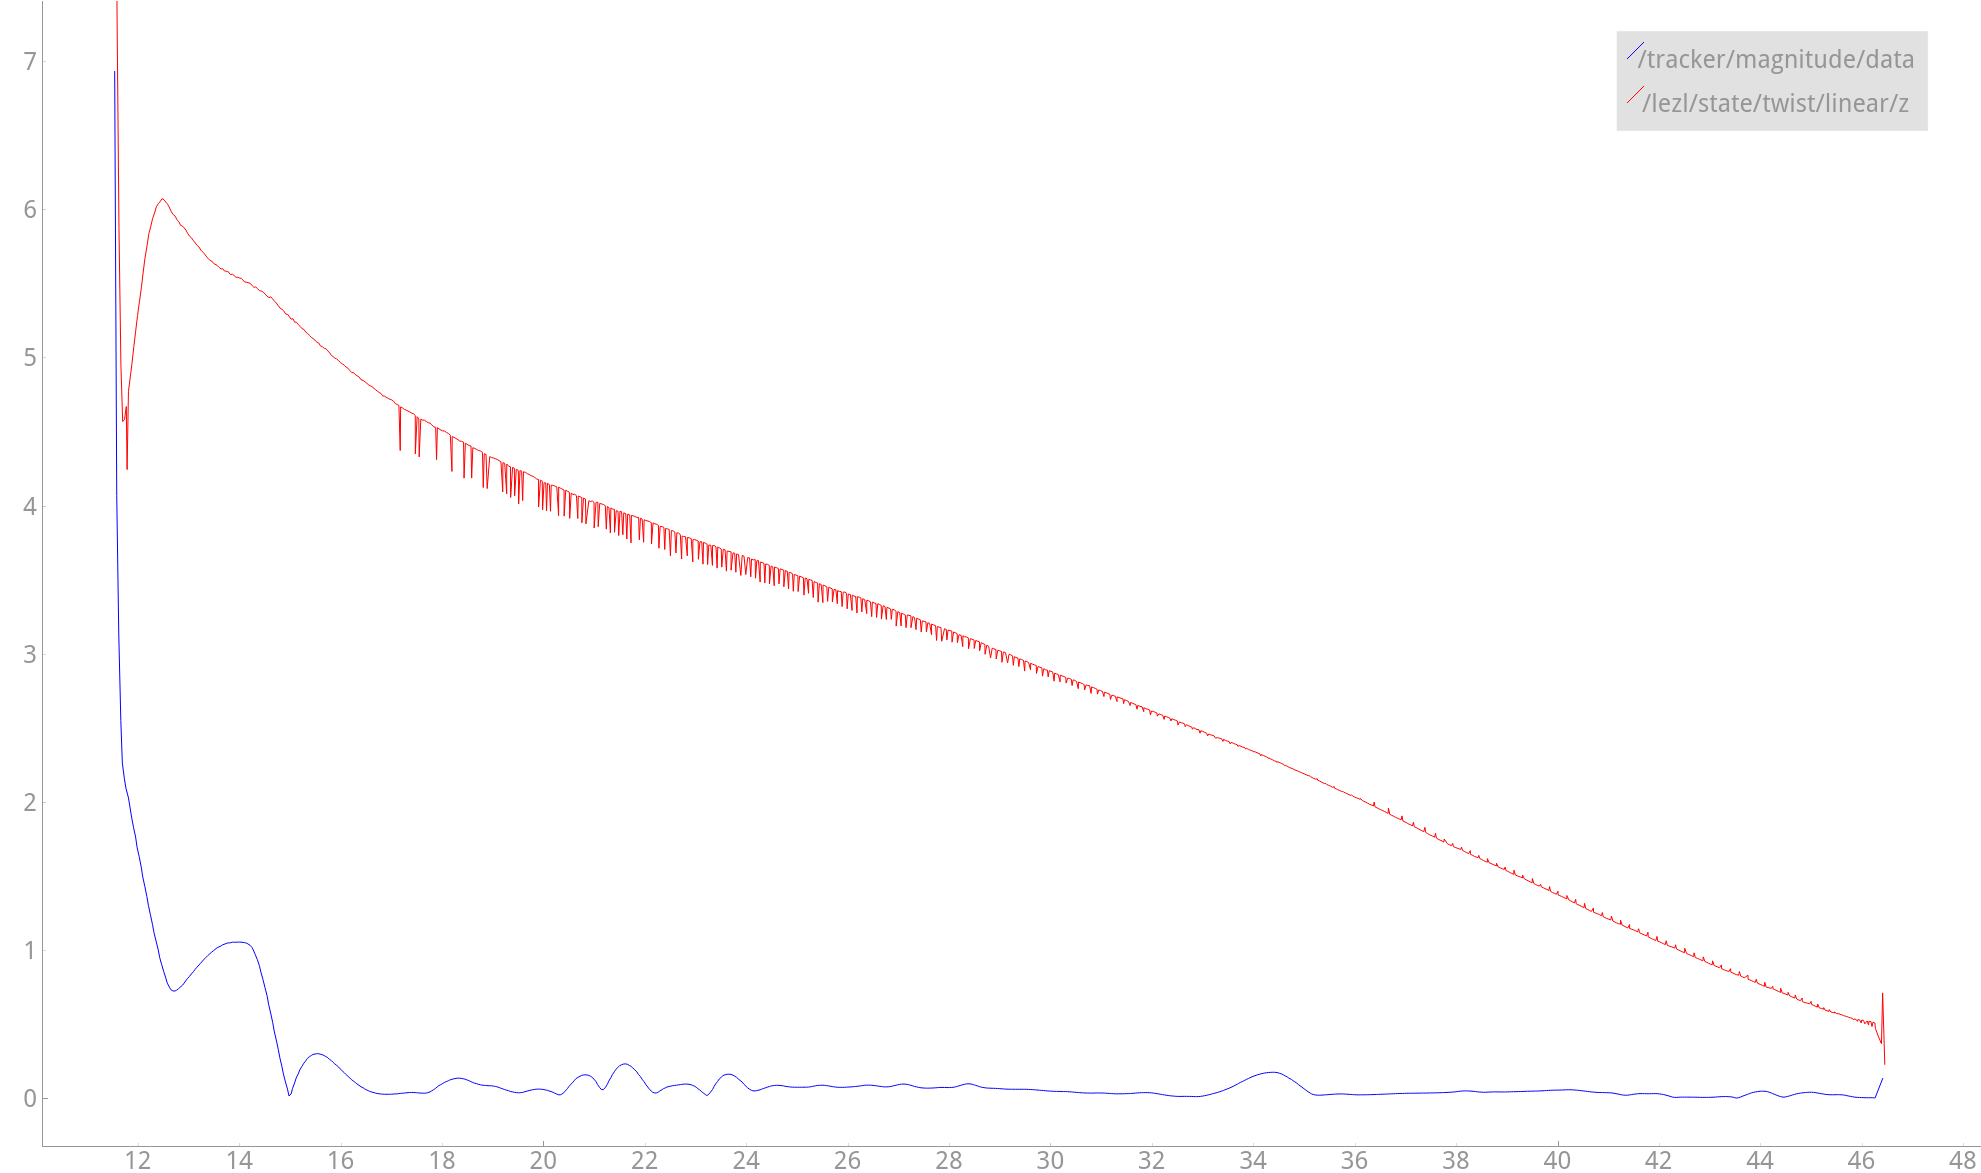
\includegraphics[width=0.9\textwidth]{images/mag_z_pid_static.png}
    \caption{$(kp,ki,kd)=(2.1,0.015,0.2)$ for static target interception.}\label{f:pid_stat}
\end{figure}

\begin{figure}
    \centering
    % GNUPLOT: LaTeX picture with Postscript
\begingroup
  \makeatletter
  \providecommand\color[2][]{%
    \GenericError{(gnuplot) \space\space\space\@spaces}{%
      Package color not loaded in conjunction with
      terminal option `colourtext'%
    }{See the gnuplot documentation for explanation.%
    }{Either use 'blacktext' in gnuplot or load the package
      color.sty in LaTeX.}%
    \renewcommand\color[2][]{}%
  }%
  \providecommand\includegraphics[2][]{%
    \GenericError{(gnuplot) \space\space\space\@spaces}{%
      Package graphicx or graphics not loaded%
    }{See the gnuplot documentation for explanation.%
    }{The gnuplot epslatex terminal needs graphicx.sty or graphics.sty.}%
    \renewcommand\includegraphics[2][]{}%
  }%
  \providecommand\rotatebox[2]{#2}%
  \@ifundefined{ifGPcolor}{%
    \newif\ifGPcolor
    \GPcolorfalse
  }{}%
  \@ifundefined{ifGPblacktext}{%
    \newif\ifGPblacktext
    \GPblacktexttrue
  }{}%
  % define a \g@addto@macro without @ in the name:
  \let\gplgaddtomacro\g@addto@macro
  % define empty templates for all commands taking text:
  \gdef\gplbacktext{}%
  \gdef\gplfronttext{}%
  \makeatother
  \ifGPblacktext
    % no textcolor at all
    \def\colorrgb#1{}%
    \def\colorgray#1{}%
  \else
    % gray or color?
    \ifGPcolor
      \def\colorrgb#1{\color[rgb]{#1}}%
      \def\colorgray#1{\color[gray]{#1}}%
      \expandafter\def\csname LTw\endcsname{\color{white}}%
      \expandafter\def\csname LTb\endcsname{\color{black}}%
      \expandafter\def\csname LTa\endcsname{\color{black}}%
      \expandafter\def\csname LT0\endcsname{\color[rgb]{1,0,0}}%
      \expandafter\def\csname LT1\endcsname{\color[rgb]{0,1,0}}%
      \expandafter\def\csname LT2\endcsname{\color[rgb]{0,0,1}}%
      \expandafter\def\csname LT3\endcsname{\color[rgb]{1,0,1}}%
      \expandafter\def\csname LT4\endcsname{\color[rgb]{0,1,1}}%
      \expandafter\def\csname LT5\endcsname{\color[rgb]{1,1,0}}%
      \expandafter\def\csname LT6\endcsname{\color[rgb]{0,0,0}}%
      \expandafter\def\csname LT7\endcsname{\color[rgb]{1,0.3,0}}%
      \expandafter\def\csname LT8\endcsname{\color[rgb]{0.5,0.5,0.5}}%
    \else
      % gray
      \def\colorrgb#1{\color{black}}%
      \def\colorgray#1{\color[gray]{#1}}%
      \expandafter\def\csname LTw\endcsname{\color{white}}%
      \expandafter\def\csname LTb\endcsname{\color{black}}%
      \expandafter\def\csname LTa\endcsname{\color{black}}%
      \expandafter\def\csname LT0\endcsname{\color{black}}%
      \expandafter\def\csname LT1\endcsname{\color{black}}%
      \expandafter\def\csname LT2\endcsname{\color{black}}%
      \expandafter\def\csname LT3\endcsname{\color{black}}%
      \expandafter\def\csname LT4\endcsname{\color{black}}%
      \expandafter\def\csname LT5\endcsname{\color{black}}%
      \expandafter\def\csname LT6\endcsname{\color{black}}%
      \expandafter\def\csname LT7\endcsname{\color{black}}%
      \expandafter\def\csname LT8\endcsname{\color{black}}%
    \fi
  \fi
    \setlength{\unitlength}{0.0500bp}%
    \ifx\gptboxheight\undefined%
      \newlength{\gptboxheight}%
      \newlength{\gptboxwidth}%
      \newsavebox{\gptboxtext}%
    \fi%
    \setlength{\fboxrule}{0.5pt}%
    \setlength{\fboxsep}{1pt}%
\begin{picture}(7200.00,5040.00)%
    \gplgaddtomacro\gplbacktext{%
      \csname LTb\endcsname%
      \put(682,704){\makebox(0,0)[r]{\strut{}$0$}}%
      \csname LTb\endcsname%
      \put(682,1111){\makebox(0,0)[r]{\strut{}$1$}}%
      \csname LTb\endcsname%
      \put(682,1518){\makebox(0,0)[r]{\strut{}$2$}}%
      \csname LTb\endcsname%
      \put(682,1925){\makebox(0,0)[r]{\strut{}$3$}}%
      \csname LTb\endcsname%
      \put(682,2332){\makebox(0,0)[r]{\strut{}$4$}}%
      \csname LTb\endcsname%
      \put(682,2740){\makebox(0,0)[r]{\strut{}$5$}}%
      \csname LTb\endcsname%
      \put(682,3147){\makebox(0,0)[r]{\strut{}$6$}}%
      \csname LTb\endcsname%
      \put(682,3554){\makebox(0,0)[r]{\strut{}$7$}}%
      \csname LTb\endcsname%
      \put(682,3961){\makebox(0,0)[r]{\strut{}$8$}}%
      \csname LTb\endcsname%
      \put(682,4368){\makebox(0,0)[r]{\strut{}$9$}}%
      \csname LTb\endcsname%
      \put(682,4775){\makebox(0,0)[r]{\strut{}$10$}}%
      \csname LTb\endcsname%
      \put(814,484){\makebox(0,0){\strut{}$10$}}%
      \csname LTb\endcsname%
      \put(1479,484){\makebox(0,0){\strut{}$15$}}%
      \csname LTb\endcsname%
      \put(2145,484){\makebox(0,0){\strut{}$20$}}%
      \csname LTb\endcsname%
      \put(2810,484){\makebox(0,0){\strut{}$25$}}%
      \csname LTb\endcsname%
      \put(3476,484){\makebox(0,0){\strut{}$30$}}%
      \csname LTb\endcsname%
      \put(4141,484){\makebox(0,0){\strut{}$35$}}%
      \csname LTb\endcsname%
      \put(4807,484){\makebox(0,0){\strut{}$40$}}%
      \csname LTb\endcsname%
      \put(5472,484){\makebox(0,0){\strut{}$45$}}%
      \csname LTb\endcsname%
      \put(6138,484){\makebox(0,0){\strut{}$50$}}%
      \csname LTb\endcsname%
      \put(6803,484){\makebox(0,0){\strut{}$55$}}%
    }%
    \gplgaddtomacro\gplfronttext{%
      \csname LTb\endcsname%
      \put(176,2739){\rotatebox{-270}{\makebox(0,0){\strut{}Error, m}}}%
      \put(3808,154){\makebox(0,0){\strut{}Time, s}}%
      \put(5816,4602){\makebox(0,0)[r]{\strut{}$e_{xy}$}}%
      \put(5816,4382){\makebox(0,0)[r]{\strut{}$e_z$}}%
    }%
    \gplbacktext
    \put(0,0){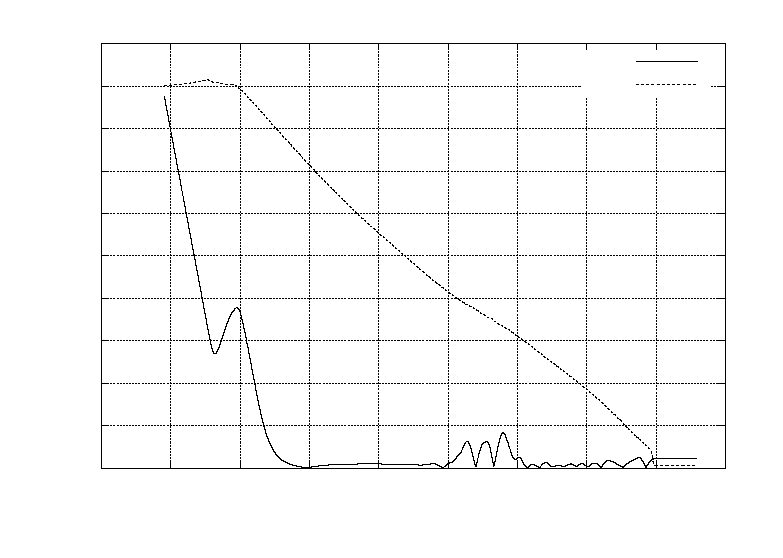
\includegraphics{pid_dyn}}%
    \gplfronttext
  \end{picture}%
\endgroup

    %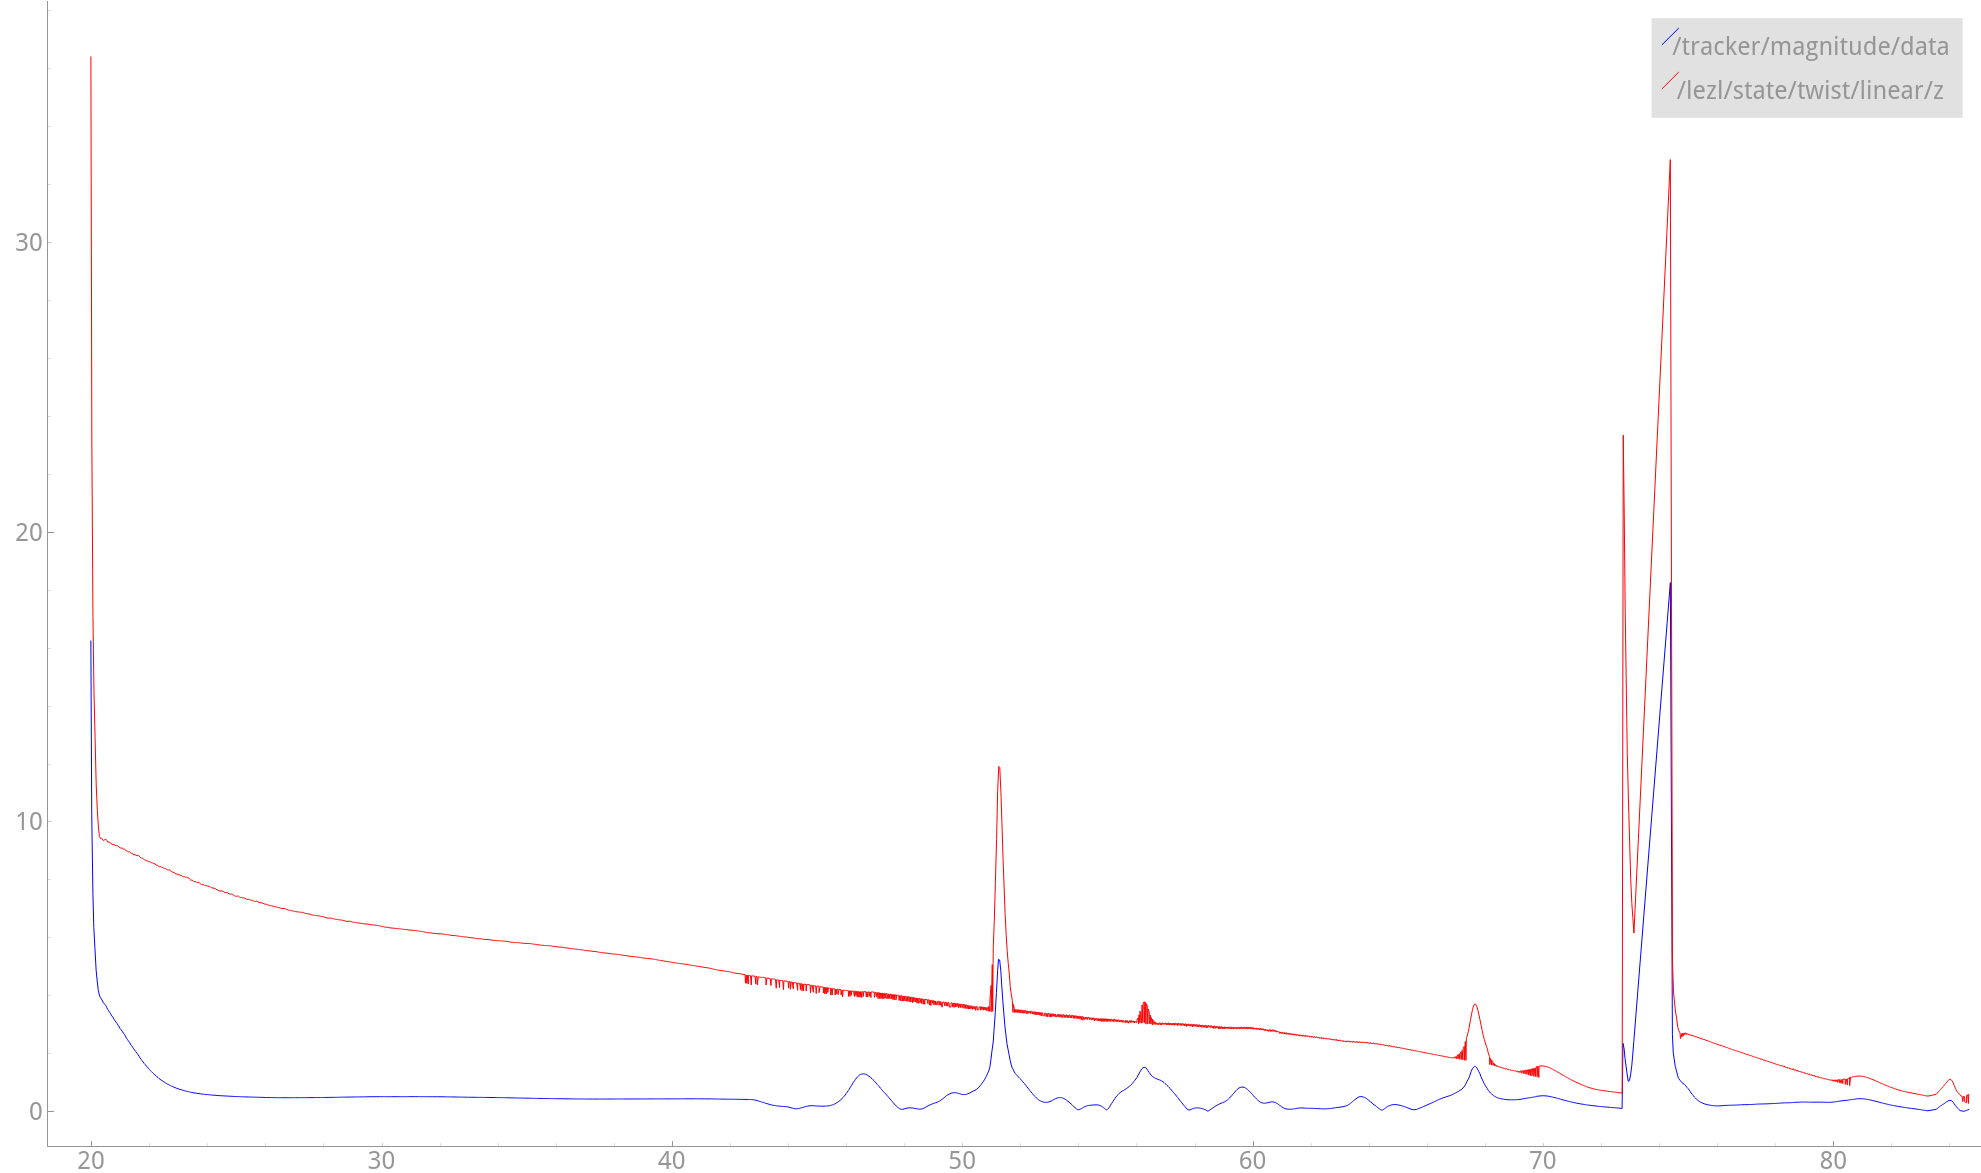
\includegraphics[width=0.9\textwidth]{images/mag_z_pid_dynamic.png}
    \caption{$(k_p,k_i,k_d)=(1.8,0.012,0.02)$ for dynamic target interception. The target is moving with a
    velocity of \SI{0.1}{\meter\per\s} in a straight line.}\label{f:pid_dyn}
\end{figure}


\subsection{Kalman Filter}\label{s:ekf}
In order to reduce the deleterious effect of instantaneous error accumulation when losing a visual track, a
kalman filter is introduced.  The filter provides a continuous, fused estimate of the vehicle's position
relative to the platform whenever there is at least visual sensing of the platform. This is done using the
\verb|robot_localization| package from ROS\cite{MooreStouchKeneralizedEkf2014}. This package is an
implementation of an extended kalman filter (EKF). The EKF provides a means by which to predict the vehicle
state even in the absence of current measurement\cite{kalman1960new}. The prediction is then corrected when
new measurement values are obtained. The measurements used to update the filter state are 1) the estimate from
the computer vision algorithm to update the vehicle position, 2) the estimate from the
AprilTag\cite{olson2011tags} routine to update both position and orientation, and 3) the IMU to
update angular rates and linear accelerations. These measurements are fused together to build an internal
model estimate of the dynamics of the vehicle. It is this model which provides the predictions between
measurements. An example of the EKF measurement is shown in \cref{f:ekf_plot}. It can be seen in this data
that though the visual estimate is very noisy, the EKF fusion follows the truth signal closely even between
the infrequent update periods of the accurate AprilTag measurement.

\begin{figure}[ht]
    \centering
    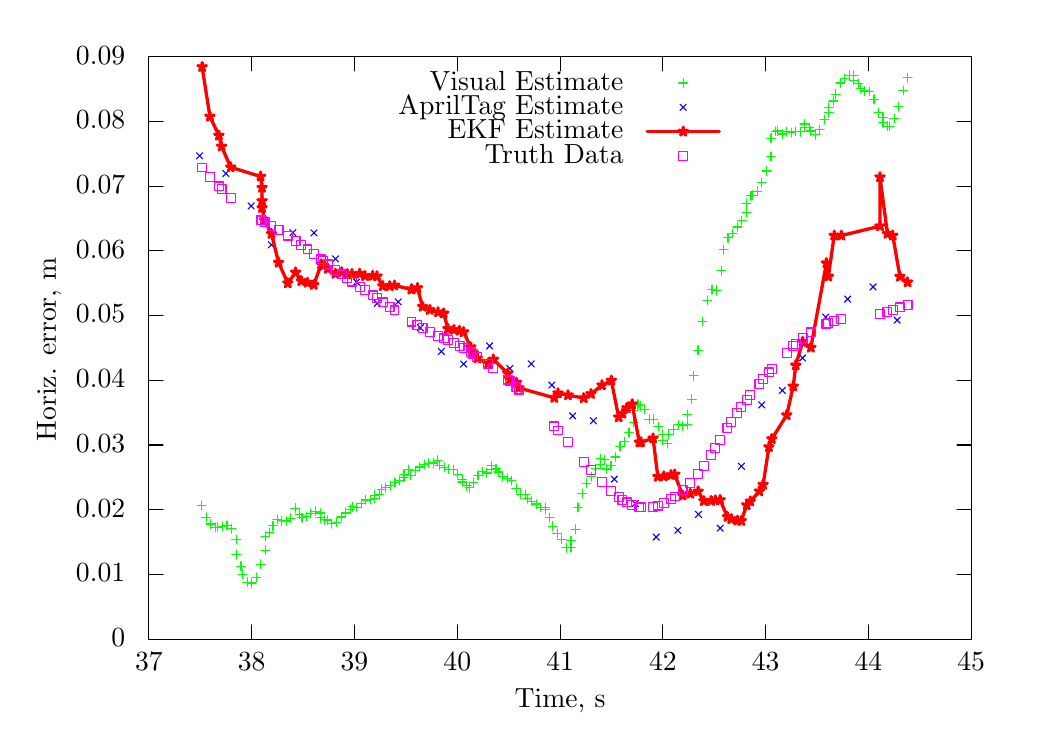
\begin{tikzpicture}[gnuplot]
%% generated with GNUPLOT 5.0p3 (Lua 5.1; terminal rev. 99, script rev. 100)
%% Mon 26 Mar 2018 04:08:56 AM EDT
\path (0.000,0.000) rectangle (12.500,8.750);
\gpcolor{color=gp lt color border}
\gpsetlinetype{gp lt border}
\gpsetdashtype{gp dt solid}
\gpsetlinewidth{1.00}
\draw[gp path] (1.504,0.985)--(1.684,0.985);
\draw[gp path] (11.947,0.985)--(11.767,0.985);
\node[gp node right] at (1.320,0.985) {$0$};
\draw[gp path] (1.504,1.807)--(1.684,1.807);
\draw[gp path] (11.947,1.807)--(11.767,1.807);
\node[gp node right] at (1.320,1.807) {$0.01$};
\draw[gp path] (1.504,2.629)--(1.684,2.629);
\draw[gp path] (11.947,2.629)--(11.767,2.629);
\node[gp node right] at (1.320,2.629) {$0.02$};
\draw[gp path] (1.504,3.450)--(1.684,3.450);
\draw[gp path] (11.947,3.450)--(11.767,3.450);
\node[gp node right] at (1.320,3.450) {$0.03$};
\draw[gp path] (1.504,4.272)--(1.684,4.272);
\draw[gp path] (11.947,4.272)--(11.767,4.272);
\node[gp node right] at (1.320,4.272) {$0.04$};
\draw[gp path] (1.504,5.094)--(1.684,5.094);
\draw[gp path] (11.947,5.094)--(11.767,5.094);
\node[gp node right] at (1.320,5.094) {$0.05$};
\draw[gp path] (1.504,5.916)--(1.684,5.916);
\draw[gp path] (11.947,5.916)--(11.767,5.916);
\node[gp node right] at (1.320,5.916) {$0.06$};
\draw[gp path] (1.504,6.737)--(1.684,6.737);
\draw[gp path] (11.947,6.737)--(11.767,6.737);
\node[gp node right] at (1.320,6.737) {$0.07$};
\draw[gp path] (1.504,7.559)--(1.684,7.559);
\draw[gp path] (11.947,7.559)--(11.767,7.559);
\node[gp node right] at (1.320,7.559) {$0.08$};
\draw[gp path] (1.504,8.381)--(1.684,8.381);
\draw[gp path] (11.947,8.381)--(11.767,8.381);
\node[gp node right] at (1.320,8.381) {$0.09$};
\draw[gp path] (1.504,0.985)--(1.504,1.165);
\draw[gp path] (1.504,8.381)--(1.504,8.201);
\node[gp node center] at (1.504,0.677) {$37$};
\draw[gp path] (2.809,0.985)--(2.809,1.165);
\draw[gp path] (2.809,8.381)--(2.809,8.201);
\node[gp node center] at (2.809,0.677) {$38$};
\draw[gp path] (4.115,0.985)--(4.115,1.165);
\draw[gp path] (4.115,8.381)--(4.115,8.201);
\node[gp node center] at (4.115,0.677) {$39$};
\draw[gp path] (5.420,0.985)--(5.420,1.165);
\draw[gp path] (5.420,8.381)--(5.420,8.201);
\node[gp node center] at (5.420,0.677) {$40$};
\draw[gp path] (6.726,0.985)--(6.726,1.165);
\draw[gp path] (6.726,8.381)--(6.726,8.201);
\node[gp node center] at (6.726,0.677) {$41$};
\draw[gp path] (8.031,0.985)--(8.031,1.165);
\draw[gp path] (8.031,8.381)--(8.031,8.201);
\node[gp node center] at (8.031,0.677) {$42$};
\draw[gp path] (9.336,0.985)--(9.336,1.165);
\draw[gp path] (9.336,8.381)--(9.336,8.201);
\node[gp node center] at (9.336,0.677) {$43$};
\draw[gp path] (10.642,0.985)--(10.642,1.165);
\draw[gp path] (10.642,8.381)--(10.642,8.201);
\node[gp node center] at (10.642,0.677) {$44$};
\draw[gp path] (11.947,0.985)--(11.947,1.165);
\draw[gp path] (11.947,8.381)--(11.947,8.201);
\node[gp node center] at (11.947,0.677) {$45$};
\draw[gp path] (1.504,8.381)--(1.504,0.985)--(11.947,0.985)--(11.947,8.381)--cycle;
\node[gp node center,rotate=-270] at (0.246,4.683) {Horiz. error, m};
\node[gp node center] at (6.725,0.215) {Time, s};
\node[gp node right] at (7.647,8.047) {Visual Estimate};
\gpcolor{rgb color={0.000,1.000,0.000}}
\gpsetpointsize{4.00}
\gppoint{gp mark 1}{(2.172,2.684)}
\gppoint{gp mark 1}{(2.230,2.531)}
\gppoint{gp mark 1}{(2.287,2.446)}
\gppoint{gp mark 1}{(2.287,2.440)}
\gppoint{gp mark 1}{(2.350,2.405)}
\gppoint{gp mark 1}{(2.377,2.406)}
\gppoint{gp mark 1}{(2.433,2.416)}
\gppoint{gp mark 1}{(2.496,2.428)}
\gppoint{gp mark 1}{(2.554,2.384)}
\gppoint{gp mark 1}{(2.611,2.249)}
\gppoint{gp mark 1}{(2.611,2.057)}
\gppoint{gp mark 1}{(2.674,1.912)}
\gppoint{gp mark 1}{(2.696,1.809)}
\gppoint{gp mark 1}{(2.752,1.709)}
\gppoint{gp mark 1}{(2.809,1.697)}
\gppoint{gp mark 1}{(2.867,1.770)}
\gppoint{gp mark 1}{(2.924,1.937)}
\gppoint{gp mark 1}{(2.982,2.115)}
\gppoint{gp mark 1}{(2.982,2.292)}
\gppoint{gp mark 1}{(3.039,2.342)}
\gppoint{gp mark 1}{(3.080,2.422)}
\gppoint{gp mark 1}{(3.132,2.506)}
\gppoint{gp mark 1}{(3.191,2.487)}
\gppoint{gp mark 1}{(3.248,2.485)}
\gppoint{gp mark 1}{(3.304,2.522)}
\gppoint{gp mark 1}{(3.362,2.646)}
\gppoint{gp mark 1}{(3.362,2.648)}
\gppoint{gp mark 1}{(3.419,2.571)}
\gppoint{gp mark 1}{(3.448,2.526)}
\gppoint{gp mark 1}{(3.503,2.540)}
\gppoint{gp mark 1}{(3.560,2.581)}
\gppoint{gp mark 1}{(3.617,2.609)}
\gppoint{gp mark 1}{(3.680,2.586)}
\gppoint{gp mark 1}{(3.680,2.525)}
\gppoint{gp mark 1}{(3.737,2.500)}
\gppoint{gp mark 1}{(3.770,2.497)}
\gppoint{gp mark 1}{(3.826,2.451)}
\gppoint{gp mark 1}{(3.884,2.469)}
\gppoint{gp mark 1}{(3.946,2.535)}
\gppoint{gp mark 1}{(4.004,2.585)}
\gppoint{gp mark 1}{(4.004,2.598)}
\gppoint{gp mark 1}{(4.061,2.632)}
\gppoint{gp mark 1}{(4.090,2.664)}
\gppoint{gp mark 1}{(4.143,2.656)}
\gppoint{gp mark 1}{(4.202,2.708)}
\gppoint{gp mark 1}{(4.260,2.752)}
\gppoint{gp mark 1}{(4.317,2.758)}
\gppoint{gp mark 1}{(4.373,2.776)}
\gppoint{gp mark 1}{(4.373,2.813)}
\gppoint{gp mark 1}{(4.432,2.817)}
\gppoint{gp mark 1}{(4.461,2.886)}
\gppoint{gp mark 1}{(4.514,2.912)}
\gppoint{gp mark 1}{(4.572,2.934)}
\gppoint{gp mark 1}{(4.629,2.972)}
\gppoint{gp mark 1}{(4.687,2.997)}
\gppoint{gp mark 1}{(4.744,3.041)}
\gppoint{gp mark 1}{(4.744,3.079)}
\gppoint{gp mark 1}{(4.801,3.139)}
\gppoint{gp mark 1}{(4.831,3.066)}
\gppoint{gp mark 1}{(4.885,3.125)}
\gppoint{gp mark 1}{(4.942,3.170)}
\gppoint{gp mark 1}{(5.000,3.201)}
\gppoint{gp mark 1}{(5.057,3.220)}
\gppoint{gp mark 1}{(5.115,3.214)}
\gppoint{gp mark 1}{(5.115,3.222)}
\gppoint{gp mark 1}{(5.172,3.258)}
\gppoint{gp mark 1}{(5.200,3.191)}
\gppoint{gp mark 1}{(5.254,3.167)}
\gppoint{gp mark 1}{(5.312,3.144)}
\gppoint{gp mark 1}{(5.369,3.135)}
\gppoint{gp mark 1}{(5.427,3.076)}
\gppoint{gp mark 1}{(5.484,3.012)}
\gppoint{gp mark 1}{(5.484,2.980)}
\gppoint{gp mark 1}{(5.542,2.930)}
\gppoint{gp mark 1}{(5.572,2.906)}
\gppoint{gp mark 1}{(5.625,2.971)}
\gppoint{gp mark 1}{(5.683,3.064)}
\gppoint{gp mark 1}{(5.740,3.113)}
\gppoint{gp mark 1}{(5.797,3.094)}
\gppoint{gp mark 1}{(5.855,3.143)}
\gppoint{gp mark 1}{(5.855,3.185)}
\gppoint{gp mark 1}{(5.912,3.145)}
\gppoint{gp mark 1}{(5.941,3.107)}
\gppoint{gp mark 1}{(5.996,3.050)}
\gppoint{gp mark 1}{(6.053,3.025)}
\gppoint{gp mark 1}{(6.111,2.998)}
\gppoint{gp mark 1}{(6.168,2.901)}
\gppoint{gp mark 1}{(6.226,2.826)}
\gppoint{gp mark 1}{(6.226,2.822)}
\gppoint{gp mark 1}{(6.283,2.816)}
\gppoint{gp mark 1}{(6.309,2.769)}
\gppoint{gp mark 1}{(6.367,2.738)}
\gppoint{gp mark 1}{(6.424,2.700)}
\gppoint{gp mark 1}{(6.480,2.659)}
\gppoint{gp mark 1}{(6.538,2.658)}
\gppoint{gp mark 1}{(6.538,2.630)}
\gppoint{gp mark 1}{(6.595,2.527)}
\gppoint{gp mark 1}{(6.633,2.420)}
\gppoint{gp mark 1}{(6.688,2.327)}
\gppoint{gp mark 1}{(6.746,2.255)}
\gppoint{gp mark 1}{(6.804,2.143)}
\gppoint{gp mark 1}{(6.865,2.149)}
\gppoint{gp mark 1}{(6.865,2.232)}
\gppoint{gp mark 1}{(6.923,2.382)}
\gppoint{gp mark 1}{(6.954,2.657)}
\gppoint{gp mark 1}{(7.006,2.832)}
\gppoint{gp mark 1}{(7.064,2.962)}
\gppoint{gp mark 1}{(7.121,3.047)}
\gppoint{gp mark 1}{(7.178,3.154)}
\gppoint{gp mark 1}{(7.236,3.202)}
\gppoint{gp mark 1}{(7.236,3.277)}
\gppoint{gp mark 1}{(7.293,3.263)}
\gppoint{gp mark 1}{(7.318,3.145)}
\gppoint{gp mark 1}{(7.372,3.187)}
\gppoint{gp mark 1}{(7.429,3.298)}
\gppoint{gp mark 1}{(7.487,3.431)}
\gppoint{gp mark 1}{(7.544,3.489)}
\gppoint{gp mark 1}{(7.601,3.608)}
\gppoint{gp mark 1}{(7.659,3.738)}
\gppoint{gp mark 1}{(7.659,3.888)}
\gppoint{gp mark 1}{(7.716,3.967)}
\gppoint{gp mark 1}{(7.744,3.947)}
\gppoint{gp mark 1}{(7.800,3.905)}
\gppoint{gp mark 1}{(7.857,3.776)}
\gppoint{gp mark 1}{(7.913,3.779)}
\gppoint{gp mark 1}{(7.971,3.684)}
\gppoint{gp mark 1}{(8.028,3.585)}
\gppoint{gp mark 1}{(8.028,3.510)}
\gppoint{gp mark 1}{(8.086,3.467)}
\gppoint{gp mark 1}{(8.108,3.586)}
\gppoint{gp mark 1}{(8.164,3.647)}
\gppoint{gp mark 1}{(8.227,3.705)}
\gppoint{gp mark 1}{(8.284,3.692)}
\gppoint{gp mark 1}{(8.342,3.707)}
\gppoint{gp mark 1}{(8.342,3.836)}
\gppoint{gp mark 1}{(8.399,4.032)}
\gppoint{gp mark 1}{(8.425,4.329)}
\gppoint{gp mark 1}{(8.477,4.655)}
\gppoint{gp mark 1}{(8.535,5.021)}
\gppoint{gp mark 1}{(8.597,5.287)}
\gppoint{gp mark 1}{(8.655,5.423)}
\gppoint{gp mark 1}{(8.712,5.408)}
\gppoint{gp mark 1}{(8.712,5.416)}
\gppoint{gp mark 1}{(8.774,5.661)}
\gppoint{gp mark 1}{(8.804,5.932)}
\gppoint{gp mark 1}{(8.858,6.080)}
\gppoint{gp mark 1}{(8.920,6.136)}
\gppoint{gp mark 1}{(8.977,6.219)}
\gppoint{gp mark 1}{(9.035,6.298)}
\gppoint{gp mark 1}{(9.092,6.406)}
\gppoint{gp mark 1}{(9.092,6.521)}
\gppoint{gp mark 1}{(9.150,6.615)}
\gppoint{gp mark 1}{(9.170,6.623)}
\gppoint{gp mark 1}{(9.228,6.673)}
\gppoint{gp mark 1}{(9.285,6.782)}
\gppoint{gp mark 1}{(9.348,6.929)}
\gppoint{gp mark 1}{(9.405,7.115)}
\gppoint{gp mark 1}{(9.405,7.348)}
\gppoint{gp mark 1}{(9.463,7.434)}
\gppoint{gp mark 1}{(9.490,7.437)}
\gppoint{gp mark 1}{(9.546,7.399)}
\gppoint{gp mark 1}{(9.604,7.430)}
\gppoint{gp mark 1}{(9.661,7.416)}
\gppoint{gp mark 1}{(9.719,7.435)}
\gppoint{gp mark 1}{(9.774,7.426)}
\gppoint{gp mark 1}{(9.831,7.484)}
\gppoint{gp mark 1}{(9.831,7.527)}
\gppoint{gp mark 1}{(9.888,7.483)}
\gppoint{gp mark 1}{(9.911,7.437)}
\gppoint{gp mark 1}{(9.967,7.388)}
\gppoint{gp mark 1}{(10.024,7.459)}
\gppoint{gp mark 1}{(10.082,7.583)}
\gppoint{gp mark 1}{(10.139,7.670)}
\gppoint{gp mark 1}{(10.139,7.737)}
\gppoint{gp mark 1}{(10.196,7.818)}
\gppoint{gp mark 1}{(10.229,7.906)}
\gppoint{gp mark 1}{(10.285,8.047)}
\gppoint{gp mark 1}{(10.343,8.102)}
\gppoint{gp mark 1}{(10.399,8.146)}
\gppoint{gp mark 1}{(10.456,8.144)}
\gppoint{gp mark 1}{(10.456,8.080)}
\gppoint{gp mark 1}{(10.514,8.041)}
\gppoint{gp mark 1}{(10.541,7.979)}
\gppoint{gp mark 1}{(10.597,7.945)}
\gppoint{gp mark 1}{(10.655,7.939)}
\gppoint{gp mark 1}{(10.712,7.842)}
\gppoint{gp mark 1}{(10.770,7.673)}
\gppoint{gp mark 1}{(10.827,7.614)}
\gppoint{gp mark 1}{(10.827,7.541)}
\gppoint{gp mark 1}{(10.884,7.500)}
\gppoint{gp mark 1}{(10.913,7.500)}
\gppoint{gp mark 1}{(10.968,7.596)}
\gppoint{gp mark 1}{(11.025,7.748)}
\gppoint{gp mark 1}{(11.083,7.952)}
\gppoint{gp mark 1}{(11.139,8.114)}
\gppoint{gp mark 1}{(8.289,8.047)}
\gpcolor{color=gp lt color border}
\node[gp node right] at (7.647,7.739) {AprilTag Estimate};
\gpcolor{rgb color={0.000,0.000,1.000}}
\gppoint{gp mark 2}{(2.148,7.123)}
\gppoint{gp mark 2}{(2.482,6.898)}
\gppoint{gp mark 2}{(2.802,6.486)}
\gppoint{gp mark 2}{(3.060,5.993)}
\gppoint{gp mark 2}{(3.332,6.146)}
\gppoint{gp mark 2}{(3.600,6.144)}
\gppoint{gp mark 2}{(3.873,5.814)}
\gppoint{gp mark 2}{(4.141,5.519)}
\gppoint{gp mark 2}{(4.405,5.249)}
\gppoint{gp mark 2}{(4.670,5.268)}
\gppoint{gp mark 2}{(4.951,4.939)}
\gppoint{gp mark 2}{(5.218,4.638)}
\gppoint{gp mark 2}{(5.501,4.478)}
\gppoint{gp mark 2}{(5.830,4.708)}
\gppoint{gp mark 2}{(6.088,4.422)}
\gppoint{gp mark 2}{(6.359,4.480)}
\gppoint{gp mark 2}{(6.621,4.211)}
\gppoint{gp mark 2}{(6.886,3.819)}
\gppoint{gp mark 2}{(7.148,3.758)}
\gppoint{gp mark 2}{(7.415,3.016)}
\gppoint{gp mark 2}{(7.681,2.705)}
\gppoint{gp mark 2}{(7.947,2.281)}
\gppoint{gp mark 2}{(8.221,2.366)}
\gppoint{gp mark 2}{(8.484,2.568)}
\gppoint{gp mark 2}{(8.759,2.394)}
\gppoint{gp mark 2}{(9.029,3.180)}
\gppoint{gp mark 2}{(9.287,3.959)}
\gppoint{gp mark 2}{(9.549,4.142)}
\gppoint{gp mark 2}{(9.806,4.556)}
\gppoint{gp mark 2}{(10.100,5.074)}
\gppoint{gp mark 2}{(10.378,5.303)}
\gppoint{gp mark 2}{(10.700,5.457)}
\gppoint{gp mark 2}{(11.007,5.035)}
\gppoint{gp mark 2}{(8.289,7.739)}
\gpcolor{color=gp lt color border}
\node[gp node right] at (7.647,7.431) {EKF Estimate};
\gpcolor{rgb color={1.000,0.000,0.000}}
\gpsetlinewidth{3.00}
\draw[gp path] (7.831,7.431)--(8.747,7.431);
\draw[gp path] (2.180,8.251)--(2.279,7.621)--(2.393,7.380)--(2.427,7.241)--(2.543,6.977)%
  --(2.922,6.860)--(2.941,6.718)--(2.941,6.549)--(2.941,6.461)--(2.973,6.302)--(3.061,6.131)%
  --(3.151,5.766)--(3.268,5.505)--(3.367,5.642)--(3.440,5.533)--(3.518,5.511)--(3.598,5.484)%
  --(3.691,5.745)--(3.718,5.730)--(3.777,5.688)--(3.873,5.625)--(3.953,5.645)--(4.022,5.622)%
  --(4.083,5.621)--(4.181,5.626)--(4.249,5.596)--(4.346,5.599)--(4.401,5.593)--(4.474,5.469)%
  --(4.561,5.469)--(4.623,5.477)--(4.839,5.425)--(4.839,5.429)--(4.914,5.444)--(4.980,5.206)%
  --(5.072,5.166)--(5.176,5.137)--(5.248,5.122)--(5.301,4.926)--(5.378,4.913)--(5.449,4.902)%
  --(5.501,4.884)--(5.591,4.693)--(5.625,4.617)--(5.675,4.550)--(5.812,4.483)--(5.878,4.536)%
  --(6.062,4.360)--(6.088,4.279)--(6.172,4.242)--(6.203,4.175)--(6.652,4.049)--(6.699,4.108)%
  --(6.826,4.083)--(7.026,4.046)--(7.118,4.099)--(7.258,4.209)--(7.377,4.268)--(7.470,3.803)%
  --(7.518,3.848)--(7.574,3.919)--(7.641,3.968)--(7.733,3.483)--(7.753,3.486)--(7.907,3.535)%
  --(7.967,3.048)--(8.043,3.052)--(8.135,3.069)--(8.182,3.077)--(8.282,2.808)--(8.379,2.832)%
  --(8.479,2.861)--(8.552,2.739)--(8.644,2.740)--(8.697,2.747)--(8.758,2.752)--(8.851,2.537)%
  --(8.900,2.509)--(8.977,2.490)--(9.027,2.486)--(9.096,2.686)--(9.142,2.734)--(9.257,2.862)%
  --(9.304,2.946)--(9.378,3.424)--(9.415,3.526)--(9.604,3.830)--(9.687,4.195)--(9.719,4.462)%
  --(9.806,4.760)--(9.911,4.687)--(10.108,5.759)--(10.133,5.590)--(10.207,6.110)--(10.298,6.110)%
  --(10.789,6.229)--(10.789,6.851)--(10.883,6.133)--(10.951,6.110)--(11.042,5.588)--(11.139,5.517);
\gppoint{gp mark 3}{(2.180,8.251)}
\gppoint{gp mark 3}{(2.279,7.621)}
\gppoint{gp mark 3}{(2.393,7.380)}
\gppoint{gp mark 3}{(2.427,7.241)}
\gppoint{gp mark 3}{(2.543,6.977)}
\gppoint{gp mark 3}{(2.922,6.860)}
\gppoint{gp mark 3}{(2.941,6.718)}
\gppoint{gp mark 3}{(2.941,6.549)}
\gppoint{gp mark 3}{(2.941,6.461)}
\gppoint{gp mark 3}{(2.973,6.302)}
\gppoint{gp mark 3}{(3.061,6.131)}
\gppoint{gp mark 3}{(3.151,5.766)}
\gppoint{gp mark 3}{(3.268,5.505)}
\gppoint{gp mark 3}{(3.367,5.642)}
\gppoint{gp mark 3}{(3.440,5.533)}
\gppoint{gp mark 3}{(3.518,5.511)}
\gppoint{gp mark 3}{(3.598,5.484)}
\gppoint{gp mark 3}{(3.691,5.745)}
\gppoint{gp mark 3}{(3.718,5.730)}
\gppoint{gp mark 3}{(3.777,5.688)}
\gppoint{gp mark 3}{(3.873,5.625)}
\gppoint{gp mark 3}{(3.953,5.645)}
\gppoint{gp mark 3}{(4.022,5.622)}
\gppoint{gp mark 3}{(4.083,5.621)}
\gppoint{gp mark 3}{(4.181,5.626)}
\gppoint{gp mark 3}{(4.249,5.596)}
\gppoint{gp mark 3}{(4.346,5.599)}
\gppoint{gp mark 3}{(4.401,5.593)}
\gppoint{gp mark 3}{(4.474,5.469)}
\gppoint{gp mark 3}{(4.561,5.469)}
\gppoint{gp mark 3}{(4.623,5.477)}
\gppoint{gp mark 3}{(4.839,5.425)}
\gppoint{gp mark 3}{(4.839,5.429)}
\gppoint{gp mark 3}{(4.914,5.444)}
\gppoint{gp mark 3}{(4.980,5.206)}
\gppoint{gp mark 3}{(5.072,5.166)}
\gppoint{gp mark 3}{(5.176,5.137)}
\gppoint{gp mark 3}{(5.248,5.122)}
\gppoint{gp mark 3}{(5.301,4.926)}
\gppoint{gp mark 3}{(5.378,4.913)}
\gppoint{gp mark 3}{(5.449,4.902)}
\gppoint{gp mark 3}{(5.501,4.884)}
\gppoint{gp mark 3}{(5.591,4.693)}
\gppoint{gp mark 3}{(5.625,4.617)}
\gppoint{gp mark 3}{(5.675,4.550)}
\gppoint{gp mark 3}{(5.812,4.483)}
\gppoint{gp mark 3}{(5.878,4.536)}
\gppoint{gp mark 3}{(6.062,4.360)}
\gppoint{gp mark 3}{(6.088,4.279)}
\gppoint{gp mark 3}{(6.172,4.242)}
\gppoint{gp mark 3}{(6.203,4.175)}
\gppoint{gp mark 3}{(6.652,4.049)}
\gppoint{gp mark 3}{(6.699,4.108)}
\gppoint{gp mark 3}{(6.826,4.083)}
\gppoint{gp mark 3}{(7.026,4.046)}
\gppoint{gp mark 3}{(7.118,4.099)}
\gppoint{gp mark 3}{(7.258,4.209)}
\gppoint{gp mark 3}{(7.377,4.268)}
\gppoint{gp mark 3}{(7.470,3.803)}
\gppoint{gp mark 3}{(7.518,3.848)}
\gppoint{gp mark 3}{(7.574,3.919)}
\gppoint{gp mark 3}{(7.641,3.968)}
\gppoint{gp mark 3}{(7.733,3.483)}
\gppoint{gp mark 3}{(7.753,3.486)}
\gppoint{gp mark 3}{(7.907,3.535)}
\gppoint{gp mark 3}{(7.967,3.048)}
\gppoint{gp mark 3}{(8.043,3.052)}
\gppoint{gp mark 3}{(8.135,3.069)}
\gppoint{gp mark 3}{(8.182,3.077)}
\gppoint{gp mark 3}{(8.282,2.808)}
\gppoint{gp mark 3}{(8.379,2.832)}
\gppoint{gp mark 3}{(8.479,2.861)}
\gppoint{gp mark 3}{(8.552,2.739)}
\gppoint{gp mark 3}{(8.644,2.740)}
\gppoint{gp mark 3}{(8.697,2.747)}
\gppoint{gp mark 3}{(8.758,2.752)}
\gppoint{gp mark 3}{(8.851,2.537)}
\gppoint{gp mark 3}{(8.900,2.509)}
\gppoint{gp mark 3}{(8.977,2.490)}
\gppoint{gp mark 3}{(9.027,2.486)}
\gppoint{gp mark 3}{(9.096,2.686)}
\gppoint{gp mark 3}{(9.142,2.734)}
\gppoint{gp mark 3}{(9.257,2.862)}
\gppoint{gp mark 3}{(9.304,2.946)}
\gppoint{gp mark 3}{(9.378,3.424)}
\gppoint{gp mark 3}{(9.415,3.526)}
\gppoint{gp mark 3}{(9.604,3.830)}
\gppoint{gp mark 3}{(9.687,4.195)}
\gppoint{gp mark 3}{(9.719,4.462)}
\gppoint{gp mark 3}{(9.806,4.760)}
\gppoint{gp mark 3}{(9.911,4.687)}
\gppoint{gp mark 3}{(10.108,5.759)}
\gppoint{gp mark 3}{(10.133,5.590)}
\gppoint{gp mark 3}{(10.207,6.110)}
\gppoint{gp mark 3}{(10.298,6.110)}
\gppoint{gp mark 3}{(10.789,6.229)}
\gppoint{gp mark 3}{(10.789,6.851)}
\gppoint{gp mark 3}{(10.883,6.133)}
\gppoint{gp mark 3}{(10.951,6.110)}
\gppoint{gp mark 3}{(11.042,5.588)}
\gppoint{gp mark 3}{(11.139,5.517)}
\gppoint{gp mark 3}{(8.289,7.431)}
\gpcolor{color=gp lt color border}
\node[gp node right] at (7.647,7.123) {Truth Data};
\gpcolor{rgb color={1.000,0.000,1.000}}
\gpsetlinewidth{1.00}
\gppoint{gp mark 4}{(2.180,6.974)}
\gppoint{gp mark 4}{(2.279,6.856)}
\gppoint{gp mark 4}{(2.393,6.734)}
\gppoint{gp mark 4}{(2.427,6.700)}
\gppoint{gp mark 4}{(2.543,6.589)}
\gppoint{gp mark 4}{(2.922,6.312)}
\gppoint{gp mark 4}{(2.941,6.301)}
\gppoint{gp mark 4}{(2.941,6.301)}
\gppoint{gp mark 4}{(2.941,6.301)}
\gppoint{gp mark 4}{(2.973,6.283)}
\gppoint{gp mark 4}{(3.061,6.232)}
\gppoint{gp mark 4}{(3.151,6.180)}
\gppoint{gp mark 4}{(3.268,6.109)}
\gppoint{gp mark 4}{(3.367,6.043)}
\gppoint{gp mark 4}{(3.440,5.991)}
\gppoint{gp mark 4}{(3.518,5.934)}
\gppoint{gp mark 4}{(3.598,5.875)}
\gppoint{gp mark 4}{(3.691,5.806)}
\gppoint{gp mark 4}{(3.718,5.786)}
\gppoint{gp mark 4}{(3.777,5.743)}
\gppoint{gp mark 4}{(3.873,5.673)}
\gppoint{gp mark 4}{(3.953,5.616)}
\gppoint{gp mark 4}{(4.022,5.567)}
\gppoint{gp mark 4}{(4.083,5.525)}
\gppoint{gp mark 4}{(4.181,5.458)}
\gppoint{gp mark 4}{(4.249,5.414)}
\gppoint{gp mark 4}{(4.346,5.350)}
\gppoint{gp mark 4}{(4.401,5.313)}
\gppoint{gp mark 4}{(4.474,5.261)}
\gppoint{gp mark 4}{(4.561,5.200)}
\gppoint{gp mark 4}{(4.623,5.159)}
\gppoint{gp mark 4}{(4.839,5.018)}
\gppoint{gp mark 4}{(4.839,5.018)}
\gppoint{gp mark 4}{(4.914,4.973)}
\gppoint{gp mark 4}{(4.980,4.935)}
\gppoint{gp mark 4}{(5.072,4.886)}
\gppoint{gp mark 4}{(5.176,4.836)}
\gppoint{gp mark 4}{(5.248,4.803)}
\gppoint{gp mark 4}{(5.301,4.779)}
\gppoint{gp mark 4}{(5.378,4.743)}
\gppoint{gp mark 4}{(5.449,4.708)}
\gppoint{gp mark 4}{(5.501,4.680)}
\gppoint{gp mark 4}{(5.591,4.625)}
\gppoint{gp mark 4}{(5.625,4.603)}
\gppoint{gp mark 4}{(5.675,4.569)}
\gppoint{gp mark 4}{(5.812,4.474)}
\gppoint{gp mark 4}{(5.878,4.425)}
\gppoint{gp mark 4}{(6.062,4.281)}
\gppoint{gp mark 4}{(6.088,4.259)}
\gppoint{gp mark 4}{(6.172,4.184)}
\gppoint{gp mark 4}{(6.203,4.154)}
\gppoint{gp mark 4}{(6.652,3.686)}
\gppoint{gp mark 4}{(6.699,3.634)}
\gppoint{gp mark 4}{(6.826,3.487)}
\gppoint{gp mark 4}{(7.026,3.238)}
\gppoint{gp mark 4}{(7.118,3.129)}
\gppoint{gp mark 4}{(7.258,2.979)}
\gppoint{gp mark 4}{(7.377,2.868)}
\gppoint{gp mark 4}{(7.470,2.791)}
\gppoint{gp mark 4}{(7.518,2.756)}
\gppoint{gp mark 4}{(7.574,2.721)}
\gppoint{gp mark 4}{(7.641,2.688)}
\gppoint{gp mark 4}{(7.733,2.660)}
\gppoint{gp mark 4}{(7.753,2.657)}
\gppoint{gp mark 4}{(7.907,2.665)}
\gppoint{gp mark 4}{(7.967,2.681)}
\gppoint{gp mark 4}{(8.043,2.712)}
\gppoint{gp mark 4}{(8.135,2.763)}
\gppoint{gp mark 4}{(8.182,2.796)}
\gppoint{gp mark 4}{(8.282,2.876)}
\gppoint{gp mark 4}{(8.379,2.970)}
\gppoint{gp mark 4}{(8.479,3.085)}
\gppoint{gp mark 4}{(8.552,3.183)}
\gppoint{gp mark 4}{(8.644,3.325)}
\gppoint{gp mark 4}{(8.697,3.411)}
\gppoint{gp mark 4}{(8.758,3.511)}
\gppoint{gp mark 4}{(8.851,3.662)}
\gppoint{gp mark 4}{(8.900,3.742)}
\gppoint{gp mark 4}{(8.977,3.859)}
\gppoint{gp mark 4}{(9.027,3.931)}
\gppoint{gp mark 4}{(9.096,4.026)}
\gppoint{gp mark 4}{(9.142,4.086)}
\gppoint{gp mark 4}{(9.257,4.229)}
\gppoint{gp mark 4}{(9.304,4.285)}
\gppoint{gp mark 4}{(9.378,4.372)}
\gppoint{gp mark 4}{(9.415,4.414)}
\gppoint{gp mark 4}{(9.604,4.622)}
\gppoint{gp mark 4}{(9.687,4.705)}
\gppoint{gp mark 4}{(9.719,4.733)}
\gppoint{gp mark 4}{(9.806,4.805)}
\gppoint{gp mark 4}{(9.911,4.879)}
\gppoint{gp mark 4}{(10.108,4.985)}
\gppoint{gp mark 4}{(10.133,4.995)}
\gppoint{gp mark 4}{(10.207,5.023)}
\gppoint{gp mark 4}{(10.298,5.049)}
\gppoint{gp mark 4}{(10.789,5.118)}
\gppoint{gp mark 4}{(10.789,5.118)}
\gppoint{gp mark 4}{(10.883,5.142)}
\gppoint{gp mark 4}{(10.951,5.164)}
\gppoint{gp mark 4}{(11.042,5.197)}
\gppoint{gp mark 4}{(11.139,5.232)}
\gppoint{gp mark 4}{(8.289,7.123)}
\gpcolor{color=gp lt color border}
\draw[gp path] (1.504,8.381)--(1.504,0.985)--(11.947,0.985)--(11.947,8.381)--cycle;
%% coordinates of the plot area
\gpdefrectangularnode{gp plot 1}{\pgfpoint{1.504cm}{0.985cm}}{\pgfpoint{11.947cm}{8.381cm}}
\end{tikzpicture}
%% gnuplot variables

    \caption{EKF estimate with input estimates over short time sample.}\label{f:ekf_plot}
\end{figure}

\Cref{app:moving} contains annotated screenshots (example in \cref{f:sim_moving_shot}) of a video of a
simulated vehicle landing on a moving platform. This video also includes a visualization of the EKF state over
time and various estimates which are fused together. A link to this video is found in the references
section\cite{yt_dyn}.

\begin{figure}
    \centering
    \includegraphics[width=0.6\textwidth]{images/moving_capture/moving-18h12m15s888.png}
    \caption{Image of the simulation environment and along with estimate visualization and camera
    feeds}\label{f:sim_moving_shot}
\end{figure}


\subsection{Fuzzy Controller}
Four fuzzy controllers of similar architecture were created as shown in \cref{f:fuzzy_mfs}.
Each input fuzzy partition was multiplied by a scaling factor to bring it into the range of the controller.
Likewise, the outputs were then again scaled to match actuation limits. The rule base was developed using
common intuition about the system dynamics. A full rule matrix was defined to fully cover the system
possibilities. This rule matrix is shown in \cref{t:rules}.
\begin{figure}[ht]
    \begin{subfigmatrix}{2}
        \subfigure[Error input \label{f:error_in_mfs}]  {\resizebox{0.48\textwidth}{!}{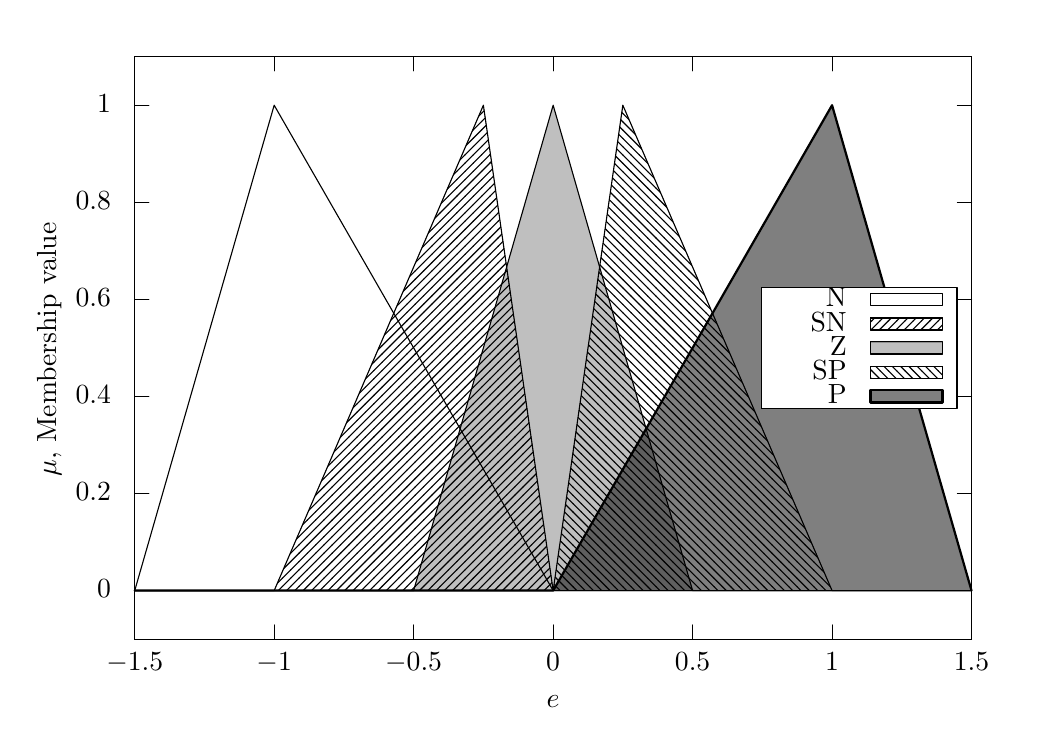
\begin{tikzpicture}[gnuplot]
%% generated with GNUPLOT 5.0p3 (Lua 5.1; terminal rev. 99, script rev. 100)
%% Wed 28 Mar 2018 11:36:11 PM EDT
\gpmonochromelines
\path (0.000,0.000) rectangle (12.500,8.750);
\gpcolor{color=gp lt color border}
\gpsetlinetype{gp lt border}
\gpsetdashtype{gp dt solid}
\gpsetlinewidth{1.00}
\draw[gp path] (1.320,1.601)--(1.500,1.601);
\draw[gp path] (11.947,1.601)--(11.767,1.601);
\node[gp node right] at (1.136,1.601) {$0$};
\draw[gp path] (1.320,2.834)--(1.500,2.834);
\draw[gp path] (11.947,2.834)--(11.767,2.834);
\node[gp node right] at (1.136,2.834) {$0.2$};
\draw[gp path] (1.320,4.067)--(1.500,4.067);
\draw[gp path] (11.947,4.067)--(11.767,4.067);
\node[gp node right] at (1.136,4.067) {$0.4$};
\draw[gp path] (1.320,5.299)--(1.500,5.299);
\draw[gp path] (11.947,5.299)--(11.767,5.299);
\node[gp node right] at (1.136,5.299) {$0.6$};
\draw[gp path] (1.320,6.532)--(1.500,6.532);
\draw[gp path] (11.947,6.532)--(11.767,6.532);
\node[gp node right] at (1.136,6.532) {$0.8$};
\draw[gp path] (1.320,7.765)--(1.500,7.765);
\draw[gp path] (11.947,7.765)--(11.767,7.765);
\node[gp node right] at (1.136,7.765) {$1$};
\draw[gp path] (1.320,0.985)--(1.320,1.165);
\draw[gp path] (1.320,8.381)--(1.320,8.201);
\node[gp node center] at (1.320,0.677) {$-1.5$};
\draw[gp path] (3.091,0.985)--(3.091,1.165);
\draw[gp path] (3.091,8.381)--(3.091,8.201);
\node[gp node center] at (3.091,0.677) {$-1$};
\draw[gp path] (4.862,0.985)--(4.862,1.165);
\draw[gp path] (4.862,8.381)--(4.862,8.201);
\node[gp node center] at (4.862,0.677) {$-0.5$};
\draw[gp path] (6.634,0.985)--(6.634,1.165);
\draw[gp path] (6.634,8.381)--(6.634,8.201);
\node[gp node center] at (6.634,0.677) {$0$};
\draw[gp path] (8.405,0.985)--(8.405,1.165);
\draw[gp path] (8.405,8.381)--(8.405,8.201);
\node[gp node center] at (8.405,0.677) {$0.5$};
\draw[gp path] (10.176,0.985)--(10.176,1.165);
\draw[gp path] (10.176,8.381)--(10.176,8.201);
\node[gp node center] at (10.176,0.677) {$1$};
\draw[gp path] (11.947,0.985)--(11.947,1.165);
\draw[gp path] (11.947,8.381)--(11.947,8.201);
\node[gp node center] at (11.947,0.677) {$1.5$};
\draw[gp path] (1.320,8.381)--(1.320,0.985)--(11.947,0.985)--(11.947,8.381)--cycle;
\node[gp node center,rotate=-270] at (0.246,4.683) {$\mu$, Membership value};
\node[gp node center] at (6.633,0.215) {$e$};
\draw[gp path] (9.283,3.913)--(9.283,5.453)--(11.763,5.453)--(11.763,3.913)--cycle;
%
  \gpfill{color=gp lt color border,gp pattern 0,pattern color=.} (1.320,1.601)--(3.091,7.765)--(6.634,1.601)--(10.176,1.601)--(11.947,1.601)--cycle;
\draw[gp path] (1.320,1.601)--(3.091,7.765)--(6.634,1.601)--(10.176,1.601)--(11.947,1.601);
\gpfill{color=gp lt color border,gp pattern 1,pattern color=.} (1.320,1.601)--(3.091,1.601)--(5.748,7.765)--(6.634,1.601)%
    --(7.519,1.601)--(10.176,1.601)--(11.947,1.601)--cycle;
\gpsetdashtype{gp dt 2}
\draw[gp path] (1.320,1.601)--(3.091,1.601)--(5.748,7.765)--(6.634,1.601)--(7.519,1.601)%
  --(10.176,1.601)--(11.947,1.601);
\gpfill{color=gp lt color border,opacity=0.25} (1.320,1.601)--(3.091,1.601)--(4.862,1.601)--(6.634,7.765)%
    --(8.405,1.601)--(10.176,1.601)--(11.947,1.601)--cycle;
\gpsetdashtype{gp dt 3}
\draw[gp path] (1.320,1.601)--(3.091,1.601)--(4.862,1.601)--(6.634,7.765)--(8.405,1.601)%
  --(10.176,1.601)--(11.947,1.601);
\gpfill{color=gp lt color border,gp pattern 2,pattern color=.} (1.320,1.601)--(3.091,1.601)--(5.748,1.601)--(6.634,1.601)%
    --(7.519,7.765)--(10.176,1.601)--(11.947,1.601)--cycle;
\gpsetdashtype{gp dt 4}
\draw[gp path] (1.320,1.601)--(3.091,1.601)--(5.748,1.601)--(6.634,1.601)--(7.519,7.765)%
  --(10.176,1.601)--(11.947,1.601);
%
  \gpfill{color=gp lt color border,opacity=0.50} (1.320,1.601)--(3.091,1.601)--(6.634,1.601)--(10.176,7.765)--(11.947,1.601)--cycle;
\gpsetlinewidth{2.00}
\draw[gp path] (1.320,1.601)--(3.091,1.601)--(6.634,1.601)--(10.176,7.765)--(11.947,1.601);
\gpfill{color=gpbgfillcolor} (9.283,3.913)--(11.763,3.913)--(11.763,5.453)--(9.283,5.453)--cycle;
\gpsetdashtype{gp dt solid}
\gpsetlinewidth{1.00}
\draw[gp path] (9.283,3.913)--(9.283,5.453)--(11.763,5.453)--(11.763,3.913)--cycle;
\node[gp node right] at (10.479,5.299) {N};
\gpfill{color=gp lt color border,gp pattern 0,pattern color=.} (10.663,5.222)--(11.579,5.222)--(11.579,5.376)--(10.663,5.376)--cycle;
\draw[gp path] (10.663,5.222)--(11.579,5.222)--(11.579,5.376)--(10.663,5.376)--cycle;
\node[gp node right] at (10.479,4.991) {SN};
\gpfill{color=gp lt color border,gp pattern 1,pattern color=.} (10.663,4.914)--(11.579,4.914)--(11.579,5.068)--(10.663,5.068)--cycle;
\gpsetdashtype{gp dt 2}
\draw[gp path] (10.663,4.914)--(11.579,4.914)--(11.579,5.068)--(10.663,5.068)--cycle;
\node[gp node right] at (10.479,4.683) {Z};
\gpfill{color=gp lt color border,opacity=0.25} (10.663,4.606)--(11.579,4.606)--(11.579,4.760)--(10.663,4.760)--cycle;
\gpsetdashtype{gp dt 3}
\draw[gp path] (10.663,4.606)--(11.579,4.606)--(11.579,4.760)--(10.663,4.760)--cycle;
\node[gp node right] at (10.479,4.375) {SP};
\gpfill{color=gp lt color border,gp pattern 2,pattern color=.} (10.663,4.298)--(11.579,4.298)--(11.579,4.452)--(10.663,4.452)--cycle;
\gpsetdashtype{gp dt 4}
\draw[gp path] (10.663,4.298)--(11.579,4.298)--(11.579,4.452)--(10.663,4.452)--cycle;
\node[gp node right] at (10.479,4.067) {P};
\gpfill{color=gp lt color border,opacity=0.50} (10.663,3.990)--(11.579,3.990)--(11.579,4.144)--(10.663,4.144)--cycle;
\gpsetlinewidth{2.00}
\draw[gp path] (10.663,3.990)--(11.579,3.990)--(11.579,4.144)--(10.663,4.144)--cycle;
\gpsetdashtype{gp dt solid}
\gpsetlinewidth{1.00}
\draw[gp path] (1.320,8.381)--(1.320,0.985)--(11.947,0.985)--(11.947,8.381)--cycle;
%% coordinates of the plot area
\gpdefrectangularnode{gp plot 1}{\pgfpoint{1.320cm}{0.985cm}}{\pgfpoint{11.947cm}{8.381cm}}
\end{tikzpicture}
%% gnuplot variables
}}
        \subfigure[Error rate input \label{f:error_d_in_mfs}]{\resizebox{0.48\textwidth}{!}{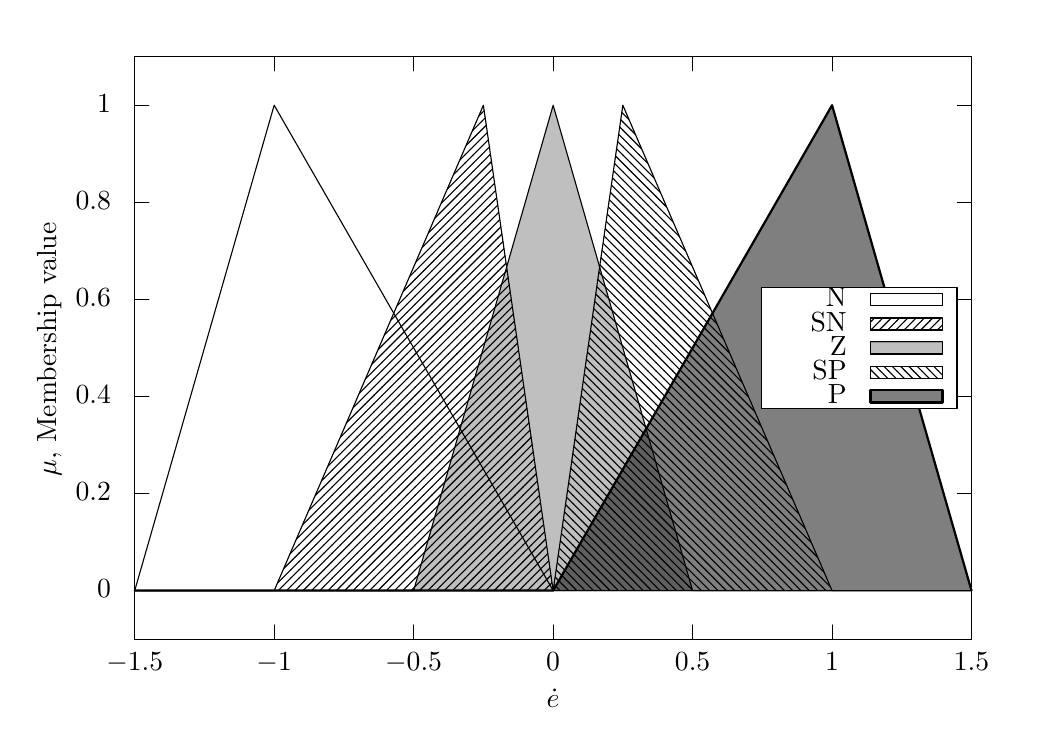
\begin{tikzpicture}[gnuplot]
%% generated with GNUPLOT 5.0p3 (Lua 5.1; terminal rev. 99, script rev. 100)
%% Wed 28 Mar 2018 11:36:11 PM EDT
\gpmonochromelines
\path (0.000,0.000) rectangle (12.500,8.750);
\gpcolor{color=gp lt color border}
\gpsetlinetype{gp lt border}
\gpsetdashtype{gp dt solid}
\gpsetlinewidth{1.00}
\draw[gp path] (1.320,1.601)--(1.500,1.601);
\draw[gp path] (11.947,1.601)--(11.767,1.601);
\node[gp node right] at (1.136,1.601) {$0$};
\draw[gp path] (1.320,2.834)--(1.500,2.834);
\draw[gp path] (11.947,2.834)--(11.767,2.834);
\node[gp node right] at (1.136,2.834) {$0.2$};
\draw[gp path] (1.320,4.067)--(1.500,4.067);
\draw[gp path] (11.947,4.067)--(11.767,4.067);
\node[gp node right] at (1.136,4.067) {$0.4$};
\draw[gp path] (1.320,5.299)--(1.500,5.299);
\draw[gp path] (11.947,5.299)--(11.767,5.299);
\node[gp node right] at (1.136,5.299) {$0.6$};
\draw[gp path] (1.320,6.532)--(1.500,6.532);
\draw[gp path] (11.947,6.532)--(11.767,6.532);
\node[gp node right] at (1.136,6.532) {$0.8$};
\draw[gp path] (1.320,7.765)--(1.500,7.765);
\draw[gp path] (11.947,7.765)--(11.767,7.765);
\node[gp node right] at (1.136,7.765) {$1$};
\draw[gp path] (1.320,0.985)--(1.320,1.165);
\draw[gp path] (1.320,8.381)--(1.320,8.201);
\node[gp node center] at (1.320,0.677) {$-1.5$};
\draw[gp path] (3.091,0.985)--(3.091,1.165);
\draw[gp path] (3.091,8.381)--(3.091,8.201);
\node[gp node center] at (3.091,0.677) {$-1$};
\draw[gp path] (4.862,0.985)--(4.862,1.165);
\draw[gp path] (4.862,8.381)--(4.862,8.201);
\node[gp node center] at (4.862,0.677) {$-0.5$};
\draw[gp path] (6.634,0.985)--(6.634,1.165);
\draw[gp path] (6.634,8.381)--(6.634,8.201);
\node[gp node center] at (6.634,0.677) {$0$};
\draw[gp path] (8.405,0.985)--(8.405,1.165);
\draw[gp path] (8.405,8.381)--(8.405,8.201);
\node[gp node center] at (8.405,0.677) {$0.5$};
\draw[gp path] (10.176,0.985)--(10.176,1.165);
\draw[gp path] (10.176,8.381)--(10.176,8.201);
\node[gp node center] at (10.176,0.677) {$1$};
\draw[gp path] (11.947,0.985)--(11.947,1.165);
\draw[gp path] (11.947,8.381)--(11.947,8.201);
\node[gp node center] at (11.947,0.677) {$1.5$};
\draw[gp path] (1.320,8.381)--(1.320,0.985)--(11.947,0.985)--(11.947,8.381)--cycle;
\node[gp node center,rotate=-270] at (0.246,4.683) {$\mu$, Membership value};
\node[gp node center] at (6.633,0.215) {$\dot{e}$};
\draw[gp path] (9.283,3.913)--(9.283,5.453)--(11.763,5.453)--(11.763,3.913)--cycle;
%
  \gpfill{color=gp lt color border,gp pattern 0,pattern color=.} (1.320,1.601)--(3.091,7.765)--(6.634,1.601)--(10.176,1.601)--(11.947,1.601)--cycle;
\draw[gp path] (1.320,1.601)--(3.091,7.765)--(6.634,1.601)--(10.176,1.601)--(11.947,1.601);
\gpfill{color=gp lt color border,gp pattern 1,pattern color=.} (1.320,1.601)--(3.091,1.601)--(5.748,7.765)--(6.634,1.601)%
    --(7.519,1.601)--(10.176,1.601)--(11.947,1.601)--cycle;
\gpsetdashtype{gp dt 2}
\draw[gp path] (1.320,1.601)--(3.091,1.601)--(5.748,7.765)--(6.634,1.601)--(7.519,1.601)%
  --(10.176,1.601)--(11.947,1.601);
\gpfill{color=gp lt color border,opacity=0.25} (1.320,1.601)--(3.091,1.601)--(4.862,1.601)--(6.634,7.765)%
    --(8.405,1.601)--(10.176,1.601)--(11.947,1.601)--cycle;
\gpsetdashtype{gp dt 3}
\draw[gp path] (1.320,1.601)--(3.091,1.601)--(4.862,1.601)--(6.634,7.765)--(8.405,1.601)%
  --(10.176,1.601)--(11.947,1.601);
\gpfill{color=gp lt color border,gp pattern 2,pattern color=.} (1.320,1.601)--(3.091,1.601)--(5.748,1.601)--(6.634,1.601)%
    --(7.519,7.765)--(10.176,1.601)--(11.947,1.601)--cycle;
\gpsetdashtype{gp dt 4}
\draw[gp path] (1.320,1.601)--(3.091,1.601)--(5.748,1.601)--(6.634,1.601)--(7.519,7.765)%
  --(10.176,1.601)--(11.947,1.601);
%
  \gpfill{color=gp lt color border,opacity=0.50} (1.320,1.601)--(3.091,1.601)--(6.634,1.601)--(10.176,7.765)--(11.947,1.601)--cycle;
\gpsetlinewidth{2.00}
\draw[gp path] (1.320,1.601)--(3.091,1.601)--(6.634,1.601)--(10.176,7.765)--(11.947,1.601);
\gpfill{color=gpbgfillcolor} (9.283,3.913)--(11.763,3.913)--(11.763,5.453)--(9.283,5.453)--cycle;
\gpsetdashtype{gp dt solid}
\gpsetlinewidth{1.00}
\draw[gp path] (9.283,3.913)--(9.283,5.453)--(11.763,5.453)--(11.763,3.913)--cycle;
\node[gp node right] at (10.479,5.299) {N};
\gpfill{color=gp lt color border,gp pattern 0,pattern color=.} (10.663,5.222)--(11.579,5.222)--(11.579,5.376)--(10.663,5.376)--cycle;
\draw[gp path] (10.663,5.222)--(11.579,5.222)--(11.579,5.376)--(10.663,5.376)--cycle;
\node[gp node right] at (10.479,4.991) {SN};
\gpfill{color=gp lt color border,gp pattern 1,pattern color=.} (10.663,4.914)--(11.579,4.914)--(11.579,5.068)--(10.663,5.068)--cycle;
\gpsetdashtype{gp dt 2}
\draw[gp path] (10.663,4.914)--(11.579,4.914)--(11.579,5.068)--(10.663,5.068)--cycle;
\node[gp node right] at (10.479,4.683) {Z};
\gpfill{color=gp lt color border,opacity=0.25} (10.663,4.606)--(11.579,4.606)--(11.579,4.760)--(10.663,4.760)--cycle;
\gpsetdashtype{gp dt 3}
\draw[gp path] (10.663,4.606)--(11.579,4.606)--(11.579,4.760)--(10.663,4.760)--cycle;
\node[gp node right] at (10.479,4.375) {SP};
\gpfill{color=gp lt color border,gp pattern 2,pattern color=.} (10.663,4.298)--(11.579,4.298)--(11.579,4.452)--(10.663,4.452)--cycle;
\gpsetdashtype{gp dt 4}
\draw[gp path] (10.663,4.298)--(11.579,4.298)--(11.579,4.452)--(10.663,4.452)--cycle;
\node[gp node right] at (10.479,4.067) {P};
\gpfill{color=gp lt color border,opacity=0.50} (10.663,3.990)--(11.579,3.990)--(11.579,4.144)--(10.663,4.144)--cycle;
\gpsetlinewidth{2.00}
\draw[gp path] (10.663,3.990)--(11.579,3.990)--(11.579,4.144)--(10.663,4.144)--cycle;
\gpsetdashtype{gp dt solid}
\gpsetlinewidth{1.00}
\draw[gp path] (1.320,8.381)--(1.320,0.985)--(11.947,0.985)--(11.947,8.381)--cycle;
%% coordinates of the plot area
\gpdefrectangularnode{gp plot 1}{\pgfpoint{1.320cm}{0.985cm}}{\pgfpoint{11.947cm}{8.381cm}}
\end{tikzpicture}
%% gnuplot variables
}}
        \subfigure[Rate command output \label{f:vel_out_mfs}]   {\resizebox{0.48\textwidth}{!}{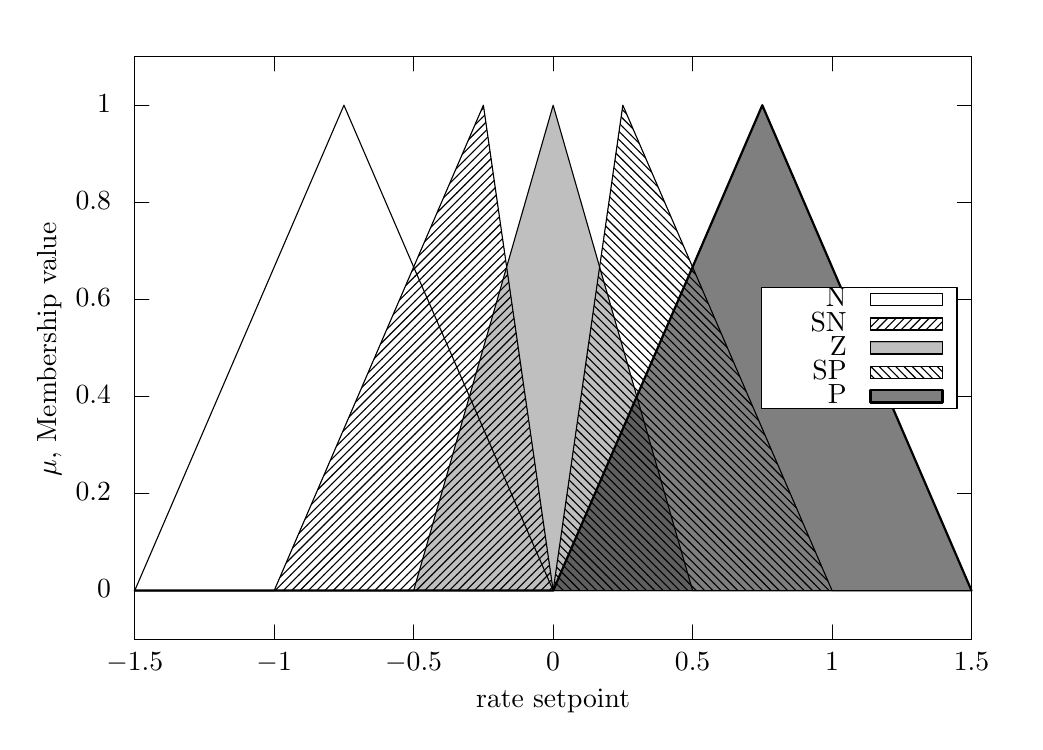
\begin{tikzpicture}[gnuplot]
%% generated with GNUPLOT 5.0p3 (Lua 5.1; terminal rev. 99, script rev. 100)
%% Wed 28 Mar 2018 11:36:11 PM EDT
\gpmonochromelines
\path (0.000,0.000) rectangle (12.500,8.750);
\gpcolor{color=gp lt color border}
\gpsetlinetype{gp lt border}
\gpsetdashtype{gp dt solid}
\gpsetlinewidth{1.00}
\draw[gp path] (1.320,1.601)--(1.500,1.601);
\draw[gp path] (11.947,1.601)--(11.767,1.601);
\node[gp node right] at (1.136,1.601) {$0$};
\draw[gp path] (1.320,2.834)--(1.500,2.834);
\draw[gp path] (11.947,2.834)--(11.767,2.834);
\node[gp node right] at (1.136,2.834) {$0.2$};
\draw[gp path] (1.320,4.067)--(1.500,4.067);
\draw[gp path] (11.947,4.067)--(11.767,4.067);
\node[gp node right] at (1.136,4.067) {$0.4$};
\draw[gp path] (1.320,5.299)--(1.500,5.299);
\draw[gp path] (11.947,5.299)--(11.767,5.299);
\node[gp node right] at (1.136,5.299) {$0.6$};
\draw[gp path] (1.320,6.532)--(1.500,6.532);
\draw[gp path] (11.947,6.532)--(11.767,6.532);
\node[gp node right] at (1.136,6.532) {$0.8$};
\draw[gp path] (1.320,7.765)--(1.500,7.765);
\draw[gp path] (11.947,7.765)--(11.767,7.765);
\node[gp node right] at (1.136,7.765) {$1$};
\draw[gp path] (1.320,0.985)--(1.320,1.165);
\draw[gp path] (1.320,8.381)--(1.320,8.201);
\node[gp node center] at (1.320,0.677) {$-1.5$};
\draw[gp path] (3.091,0.985)--(3.091,1.165);
\draw[gp path] (3.091,8.381)--(3.091,8.201);
\node[gp node center] at (3.091,0.677) {$-1$};
\draw[gp path] (4.862,0.985)--(4.862,1.165);
\draw[gp path] (4.862,8.381)--(4.862,8.201);
\node[gp node center] at (4.862,0.677) {$-0.5$};
\draw[gp path] (6.634,0.985)--(6.634,1.165);
\draw[gp path] (6.634,8.381)--(6.634,8.201);
\node[gp node center] at (6.634,0.677) {$0$};
\draw[gp path] (8.405,0.985)--(8.405,1.165);
\draw[gp path] (8.405,8.381)--(8.405,8.201);
\node[gp node center] at (8.405,0.677) {$0.5$};
\draw[gp path] (10.176,0.985)--(10.176,1.165);
\draw[gp path] (10.176,8.381)--(10.176,8.201);
\node[gp node center] at (10.176,0.677) {$1$};
\draw[gp path] (11.947,0.985)--(11.947,1.165);
\draw[gp path] (11.947,8.381)--(11.947,8.201);
\node[gp node center] at (11.947,0.677) {$1.5$};
\draw[gp path] (1.320,8.381)--(1.320,0.985)--(11.947,0.985)--(11.947,8.381)--cycle;
\node[gp node center,rotate=-270] at (0.246,4.683) {$\mu$, Membership value};
\node[gp node center] at (6.633,0.215) {rate setpoint};
\draw[gp path] (9.283,3.913)--(9.283,5.453)--(11.763,5.453)--(11.763,3.913)--cycle;
\gpfill{color=gp lt color border,gp pattern 0,pattern color=.} (1.320,1.601)--(3.977,7.765)--(6.634,1.601)--(11.947,1.601)--cycle;
\draw[gp path] (1.320,1.601)--(3.977,7.765)--(6.634,1.601)--(11.947,1.601);
%
  \gpfill{color=gp lt color border,gp pattern 1,pattern color=.} (1.320,1.601)--(3.091,1.601)--(5.748,7.765)--(6.634,1.601)--(11.947,1.601)--cycle;
\gpsetdashtype{gp dt 2}
\draw[gp path] (1.320,1.601)--(3.091,1.601)--(5.748,7.765)--(6.634,1.601)--(11.947,1.601);
%
  \gpfill{color=gp lt color border,opacity=0.25} (1.320,1.601)--(4.862,1.601)--(6.634,7.765)--(8.405,1.601)--(11.947,1.601)--cycle;
\gpsetdashtype{gp dt 3}
\draw[gp path] (1.320,1.601)--(4.862,1.601)--(6.634,7.765)--(8.405,1.601)--(11.947,1.601);
%
  \gpfill{color=gp lt color border,gp pattern 2,pattern color=.} (1.320,1.601)--(6.634,1.601)--(7.519,7.765)--(10.176,1.601)--(11.947,1.601)--cycle;
\gpsetdashtype{gp dt 4}
\draw[gp path] (1.320,1.601)--(6.634,1.601)--(7.519,7.765)--(10.176,1.601)--(11.947,1.601);
\gpfill{color=gp lt color border,opacity=0.50} (1.320,1.601)--(6.634,1.601)--(9.290,7.765)--(11.947,1.601)--cycle;
\gpsetlinewidth{2.00}
\draw[gp path] (1.320,1.601)--(6.634,1.601)--(9.290,7.765)--(11.947,1.601);
\gpfill{color=gpbgfillcolor} (9.283,3.913)--(11.763,3.913)--(11.763,5.453)--(9.283,5.453)--cycle;
\gpsetdashtype{gp dt solid}
\gpsetlinewidth{1.00}
\draw[gp path] (9.283,3.913)--(9.283,5.453)--(11.763,5.453)--(11.763,3.913)--cycle;
\node[gp node right] at (10.479,5.299) {N};
\gpfill{color=gp lt color border,gp pattern 0,pattern color=.} (10.663,5.222)--(11.579,5.222)--(11.579,5.376)--(10.663,5.376)--cycle;
\draw[gp path] (10.663,5.222)--(11.579,5.222)--(11.579,5.376)--(10.663,5.376)--cycle;
\node[gp node right] at (10.479,4.991) {SN};
\gpfill{color=gp lt color border,gp pattern 1,pattern color=.} (10.663,4.914)--(11.579,4.914)--(11.579,5.068)--(10.663,5.068)--cycle;
\gpsetdashtype{gp dt 2}
\draw[gp path] (10.663,4.914)--(11.579,4.914)--(11.579,5.068)--(10.663,5.068)--cycle;
\node[gp node right] at (10.479,4.683) {Z};
\gpfill{color=gp lt color border,opacity=0.25} (10.663,4.606)--(11.579,4.606)--(11.579,4.760)--(10.663,4.760)--cycle;
\gpsetdashtype{gp dt 3}
\draw[gp path] (10.663,4.606)--(11.579,4.606)--(11.579,4.760)--(10.663,4.760)--cycle;
\node[gp node right] at (10.479,4.375) {SP};
\gpfill{color=gp lt color border,gp pattern 2,pattern color=.} (10.663,4.298)--(11.579,4.298)--(11.579,4.452)--(10.663,4.452)--cycle;
\gpsetdashtype{gp dt 4}
\draw[gp path] (10.663,4.298)--(11.579,4.298)--(11.579,4.452)--(10.663,4.452)--cycle;
\node[gp node right] at (10.479,4.067) {P};
\gpfill{color=gp lt color border,opacity=0.50} (10.663,3.990)--(11.579,3.990)--(11.579,4.144)--(10.663,4.144)--cycle;
\gpsetlinewidth{2.00}
\draw[gp path] (10.663,3.990)--(11.579,3.990)--(11.579,4.144)--(10.663,4.144)--cycle;
\gpsetdashtype{gp dt solid}
\gpsetlinewidth{1.00}
\draw[gp path] (1.320,8.381)--(1.320,0.985)--(11.947,0.985)--(11.947,8.381)--cycle;
%% coordinates of the plot area
\gpdefrectangularnode{gp plot 1}{\pgfpoint{1.320cm}{0.985cm}}{\pgfpoint{11.947cm}{8.381cm}}
\end{tikzpicture}
%% gnuplot variables
}}
    \end{subfigmatrix}
    \caption{Membership function definitions for fuzzy logic controller.}\label{f:fuzzy_mfs}
\end{figure}

These rules provide a process by which to lend the controller a
decision-making system with a foundation in human reasoning. The tuning process of the fuzzy controller then
becomes the task of defining the membership functions which decide how much of each rule should be activated
for certain inputs. Triangular membership functions are used exclusively for their simplicity in definition
and tuning\cite{mishra1994performance} while the aggregation of rules is the popular min-max method put forth
by Mamdani\cite{MAMDANI19751}. The membership functions shown in \cref{f:fuzzy_mfs} are the result of a number
of iterative tuning steps and were found to be the most effective of the configurations attempted.


\begin{table}[ht]
    \centering
    \caption{Fuzzy rule base. The error and error rate membership sets correspond to velocity output
    membership sets according to this table. N-negative, SN-small negative, Z-zero, SP-small positive,
P-positive}re intuitive and easy to understand and pr\label{t:rules}
    \begin{tabular}{cc||c|c|c|c|c|}
        &  \multicolumn{6}{c}{error}  \\ 	
        \multirow{6}{*}{error rate} &    & N  & SN & Z  & SP & P  \\ 	\hhline{~=#=|=|=|=|=|}
                                    & N  & P  & P  & SP & SP & Z  \\ 	\cline{2-7}
                                    & SN & P  & SP & SP & Z  & SN \\ 	\cline{2-7}
                                    & Z  & SP & SP & Z  & SN & SN \\ 	\cline{2-7}
                                    & SP & SP & Z  & SN & SN & N  \\ 	\cline{2-7}
                                    & P  & Z  & SN & SN & N  & N  \\ 	\cline{2-7}
    \end{tabular}
\end{table}



The result of this controller was sufficient to land the quadrotor on both the static and
constant linear velocity dynamic platforms. \Crefrange{f:fuz_stat}{f:fuz_dyn} show the results of the static
and dynamic landings using the fuzzy controllers. These figures begin at takeoff of the vehicle, and it is
clearly seen where the controller locks onto the visual image and initiates the landing state. It is also
clearly seen that with the implementation of both the kalman filter and the fuzzy controller, the errors
resulting from image loss are eliminated, providing a smoother landing approach.

\begin{figure}
    \centering
    % GNUPLOT: LaTeX picture with Postscript
\begingroup
  \makeatletter
  \providecommand\color[2][]{%
    \GenericError{(gnuplot) \space\space\space\@spaces}{%
      Package color not loaded in conjunction with
      terminal option `colourtext'%
    }{See the gnuplot documentation for explanation.%
    }{Either use 'blacktext' in gnuplot or load the package
      color.sty in LaTeX.}%
    \renewcommand\color[2][]{}%
  }%
  \providecommand\includegraphics[2][]{%
    \GenericError{(gnuplot) \space\space\space\@spaces}{%
      Package graphicx or graphics not loaded%
    }{See the gnuplot documentation for explanation.%
    }{The gnuplot epslatex terminal needs graphicx.sty or graphics.sty.}%
    \renewcommand\includegraphics[2][]{}%
  }%
  \providecommand\rotatebox[2]{#2}%
  \@ifundefined{ifGPcolor}{%
    \newif\ifGPcolor
    \GPcolorfalse
  }{}%
  \@ifundefined{ifGPblacktext}{%
    \newif\ifGPblacktext
    \GPblacktexttrue
  }{}%
  % define a \g@addto@macro without @ in the name:
  \let\gplgaddtomacro\g@addto@macro
  % define empty templates for all commands taking text:
  \gdef\gplbacktext{}%
  \gdef\gplfronttext{}%
  \makeatother
  \ifGPblacktext
    % no textcolor at all
    \def\colorrgb#1{}%
    \def\colorgray#1{}%
  \else
    % gray or color?
    \ifGPcolor
      \def\colorrgb#1{\color[rgb]{#1}}%
      \def\colorgray#1{\color[gray]{#1}}%
      \expandafter\def\csname LTw\endcsname{\color{white}}%
      \expandafter\def\csname LTb\endcsname{\color{black}}%
      \expandafter\def\csname LTa\endcsname{\color{black}}%
      \expandafter\def\csname LT0\endcsname{\color[rgb]{1,0,0}}%
      \expandafter\def\csname LT1\endcsname{\color[rgb]{0,1,0}}%
      \expandafter\def\csname LT2\endcsname{\color[rgb]{0,0,1}}%
      \expandafter\def\csname LT3\endcsname{\color[rgb]{1,0,1}}%
      \expandafter\def\csname LT4\endcsname{\color[rgb]{0,1,1}}%
      \expandafter\def\csname LT5\endcsname{\color[rgb]{1,1,0}}%
      \expandafter\def\csname LT6\endcsname{\color[rgb]{0,0,0}}%
      \expandafter\def\csname LT7\endcsname{\color[rgb]{1,0.3,0}}%
      \expandafter\def\csname LT8\endcsname{\color[rgb]{0.5,0.5,0.5}}%
    \else
      % gray
      \def\colorrgb#1{\color{black}}%
      \def\colorgray#1{\color[gray]{#1}}%
      \expandafter\def\csname LTw\endcsname{\color{white}}%
      \expandafter\def\csname LTb\endcsname{\color{black}}%
      \expandafter\def\csname LTa\endcsname{\color{black}}%
      \expandafter\def\csname LT0\endcsname{\color{black}}%
      \expandafter\def\csname LT1\endcsname{\color{black}}%
      \expandafter\def\csname LT2\endcsname{\color{black}}%
      \expandafter\def\csname LT3\endcsname{\color{black}}%
      \expandafter\def\csname LT4\endcsname{\color{black}}%
      \expandafter\def\csname LT5\endcsname{\color{black}}%
      \expandafter\def\csname LT6\endcsname{\color{black}}%
      \expandafter\def\csname LT7\endcsname{\color{black}}%
      \expandafter\def\csname LT8\endcsname{\color{black}}%
    \fi
  \fi
    \setlength{\unitlength}{0.0500bp}%
    \ifx\gptboxheight\undefined%
      \newlength{\gptboxheight}%
      \newlength{\gptboxwidth}%
      \newsavebox{\gptboxtext}%
    \fi%
    \setlength{\fboxrule}{0.5pt}%
    \setlength{\fboxsep}{1pt}%
\begin{picture}(7200.00,5040.00)%
    \gplgaddtomacro\gplbacktext{%
      \csname LTb\endcsname%
      \put(946,704){\makebox(0,0)[r]{\strut{}$-0.5$}}%
      \csname LTb\endcsname%
      \put(946,1111){\makebox(0,0)[r]{\strut{}$0$}}%
      \csname LTb\endcsname%
      \put(946,1518){\makebox(0,0)[r]{\strut{}$0.5$}}%
      \csname LTb\endcsname%
      \put(946,1925){\makebox(0,0)[r]{\strut{}$1$}}%
      \csname LTb\endcsname%
      \put(946,2332){\makebox(0,0)[r]{\strut{}$1.5$}}%
      \csname LTb\endcsname%
      \put(946,2740){\makebox(0,0)[r]{\strut{}$2$}}%
      \csname LTb\endcsname%
      \put(946,3147){\makebox(0,0)[r]{\strut{}$2.5$}}%
      \csname LTb\endcsname%
      \put(946,3554){\makebox(0,0)[r]{\strut{}$3$}}%
      \csname LTb\endcsname%
      \put(946,3961){\makebox(0,0)[r]{\strut{}$3.5$}}%
      \csname LTb\endcsname%
      \put(946,4368){\makebox(0,0)[r]{\strut{}$4$}}%
      \csname LTb\endcsname%
      \put(946,4775){\makebox(0,0)[r]{\strut{}$4.5$}}%
      \csname LTb\endcsname%
      \put(1078,484){\makebox(0,0){\strut{}$0$}}%
      \csname LTb\endcsname%
      \put(1896,484){\makebox(0,0){\strut{}$5$}}%
      \csname LTb\endcsname%
      \put(2714,484){\makebox(0,0){\strut{}$10$}}%
      \csname LTb\endcsname%
      \put(3532,484){\makebox(0,0){\strut{}$15$}}%
      \csname LTb\endcsname%
      \put(4349,484){\makebox(0,0){\strut{}$20$}}%
      \csname LTb\endcsname%
      \put(5167,484){\makebox(0,0){\strut{}$25$}}%
      \csname LTb\endcsname%
      \put(5985,484){\makebox(0,0){\strut{}$30$}}%
      \csname LTb\endcsname%
      \put(6803,484){\makebox(0,0){\strut{}$35$}}%
    }%
    \gplgaddtomacro\gplfronttext{%
      \csname LTb\endcsname%
      \put(176,2739){\rotatebox{-270}{\makebox(0,0){\strut{}Error, m}}}%
      \put(3940,154){\makebox(0,0){\strut{}Time, s}}%
      \put(5816,4602){\makebox(0,0)[r]{\strut{}$e_{xy}$}}%
      \put(5816,4382){\makebox(0,0)[r]{\strut{}$e_z$}}%
    }%
    \gplbacktext
    \put(0,0){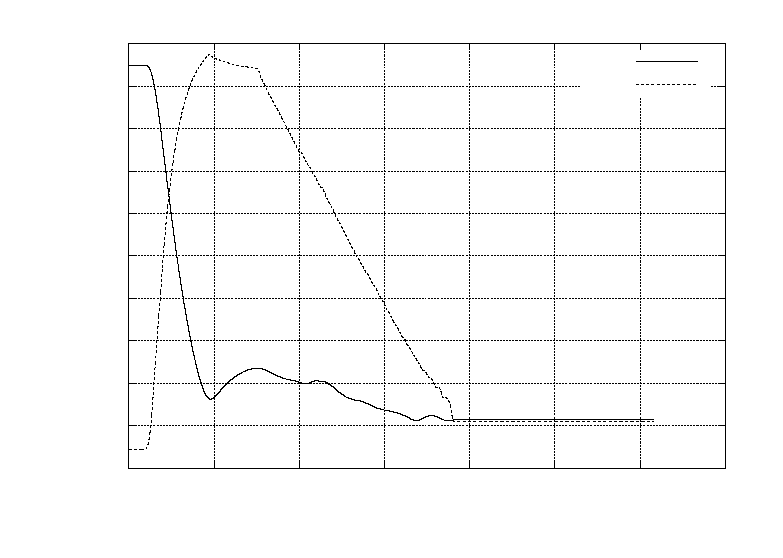
\includegraphics{static_smach_good_plot}}%
    \gplfronttext
  \end{picture}%
\endgroup

    \caption{Fuzzy-controlled static target interception.}\label{f:fuz_stat}
\end{figure}

\begin{figure}
    \centering
    % GNUPLOT: LaTeX picture with Postscript
\begingroup
  \makeatletter
  \providecommand\color[2][]{%
    \GenericError{(gnuplot) \space\space\space\@spaces}{%
      Package color not loaded in conjunction with
      terminal option `colourtext'%
    }{See the gnuplot documentation for explanation.%
    }{Either use 'blacktext' in gnuplot or load the package
      color.sty in LaTeX.}%
    \renewcommand\color[2][]{}%
  }%
  \providecommand\includegraphics[2][]{%
    \GenericError{(gnuplot) \space\space\space\@spaces}{%
      Package graphicx or graphics not loaded%
    }{See the gnuplot documentation for explanation.%
    }{The gnuplot epslatex terminal needs graphicx.sty or graphics.sty.}%
    \renewcommand\includegraphics[2][]{}%
  }%
  \providecommand\rotatebox[2]{#2}%
  \@ifundefined{ifGPcolor}{%
    \newif\ifGPcolor
    \GPcolorfalse
  }{}%
  \@ifundefined{ifGPblacktext}{%
    \newif\ifGPblacktext
    \GPblacktexttrue
  }{}%
  % define a \g@addto@macro without @ in the name:
  \let\gplgaddtomacro\g@addto@macro
  % define empty templates for all commands taking text:
  \gdef\gplbacktext{}%
  \gdef\gplfronttext{}%
  \makeatother
  \ifGPblacktext
    % no textcolor at all
    \def\colorrgb#1{}%
    \def\colorgray#1{}%
  \else
    % gray or color?
    \ifGPcolor
      \def\colorrgb#1{\color[rgb]{#1}}%
      \def\colorgray#1{\color[gray]{#1}}%
      \expandafter\def\csname LTw\endcsname{\color{white}}%
      \expandafter\def\csname LTb\endcsname{\color{black}}%
      \expandafter\def\csname LTa\endcsname{\color{black}}%
      \expandafter\def\csname LT0\endcsname{\color[rgb]{1,0,0}}%
      \expandafter\def\csname LT1\endcsname{\color[rgb]{0,1,0}}%
      \expandafter\def\csname LT2\endcsname{\color[rgb]{0,0,1}}%
      \expandafter\def\csname LT3\endcsname{\color[rgb]{1,0,1}}%
      \expandafter\def\csname LT4\endcsname{\color[rgb]{0,1,1}}%
      \expandafter\def\csname LT5\endcsname{\color[rgb]{1,1,0}}%
      \expandafter\def\csname LT6\endcsname{\color[rgb]{0,0,0}}%
      \expandafter\def\csname LT7\endcsname{\color[rgb]{1,0.3,0}}%
      \expandafter\def\csname LT8\endcsname{\color[rgb]{0.5,0.5,0.5}}%
    \else
      % gray
      \def\colorrgb#1{\color{black}}%
      \def\colorgray#1{\color[gray]{#1}}%
      \expandafter\def\csname LTw\endcsname{\color{white}}%
      \expandafter\def\csname LTb\endcsname{\color{black}}%
      \expandafter\def\csname LTa\endcsname{\color{black}}%
      \expandafter\def\csname LT0\endcsname{\color{black}}%
      \expandafter\def\csname LT1\endcsname{\color{black}}%
      \expandafter\def\csname LT2\endcsname{\color{black}}%
      \expandafter\def\csname LT3\endcsname{\color{black}}%
      \expandafter\def\csname LT4\endcsname{\color{black}}%
      \expandafter\def\csname LT5\endcsname{\color{black}}%
      \expandafter\def\csname LT6\endcsname{\color{black}}%
      \expandafter\def\csname LT7\endcsname{\color{black}}%
      \expandafter\def\csname LT8\endcsname{\color{black}}%
    \fi
  \fi
    \setlength{\unitlength}{0.0500bp}%
    \ifx\gptboxheight\undefined%
      \newlength{\gptboxheight}%
      \newlength{\gptboxwidth}%
      \newsavebox{\gptboxtext}%
    \fi%
    \setlength{\fboxrule}{0.5pt}%
    \setlength{\fboxsep}{1pt}%
\begin{picture}(7200.00,5040.00)%
    \gplgaddtomacro\gplbacktext{%
      \csname LTb\endcsname%
      \put(682,704){\makebox(0,0)[r]{\strut{}$-1$}}%
      \csname LTb\endcsname%
      \put(682,1213){\makebox(0,0)[r]{\strut{}$0$}}%
      \csname LTb\endcsname%
      \put(682,1722){\makebox(0,0)[r]{\strut{}$1$}}%
      \csname LTb\endcsname%
      \put(682,2231){\makebox(0,0)[r]{\strut{}$2$}}%
      \csname LTb\endcsname%
      \put(682,2740){\makebox(0,0)[r]{\strut{}$3$}}%
      \csname LTb\endcsname%
      \put(682,3248){\makebox(0,0)[r]{\strut{}$4$}}%
      \csname LTb\endcsname%
      \put(682,3757){\makebox(0,0)[r]{\strut{}$5$}}%
      \csname LTb\endcsname%
      \put(682,4266){\makebox(0,0)[r]{\strut{}$6$}}%
      \csname LTb\endcsname%
      \put(682,4775){\makebox(0,0)[r]{\strut{}$7$}}%
      \csname LTb\endcsname%
      \put(814,484){\makebox(0,0){\strut{}$0$}}%
      \csname LTb\endcsname%
      \put(2012,484){\makebox(0,0){\strut{}$5$}}%
      \csname LTb\endcsname%
      \put(3210,484){\makebox(0,0){\strut{}$10$}}%
      \csname LTb\endcsname%
      \put(4407,484){\makebox(0,0){\strut{}$15$}}%
      \csname LTb\endcsname%
      \put(5605,484){\makebox(0,0){\strut{}$20$}}%
      \csname LTb\endcsname%
      \put(6803,484){\makebox(0,0){\strut{}$25$}}%
    }%
    \gplgaddtomacro\gplfronttext{%
      \csname LTb\endcsname%
      \put(176,2739){\rotatebox{-270}{\makebox(0,0){\strut{}Error, m}}}%
      \put(3808,154){\makebox(0,0){\strut{}Time, s}}%
      \put(5816,4602){\makebox(0,0)[r]{\strut{}$e_{xy}$}}%
      \put(5816,4382){\makebox(0,0)[r]{\strut{}$e_z$}}%
    }%
    \gplbacktext
    \put(0,0){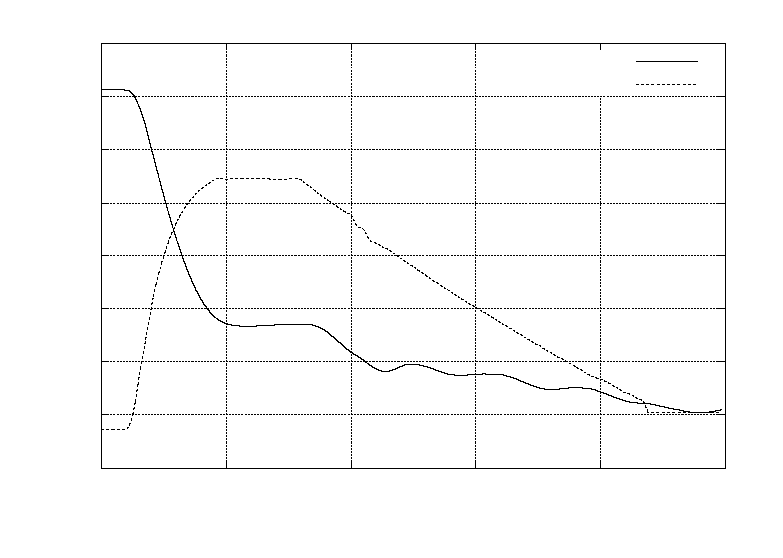
\includegraphics{moving_line_good_plot}}%
    \gplfronttext
  \end{picture}%
\endgroup

    \caption{Fuzzy-controlled dynamic target interception. The target is moving in a straight line with a
    velocity of \SI{0.1}{\meter\per\second}.}\label{f:fuz_dyn}
\end{figure}


%\begin{figure}[ht]
    %\centering
    %\begin{subfigmatrix}{2}
        %\subfigure[Static target interception.\label{f:fuz_stat}]{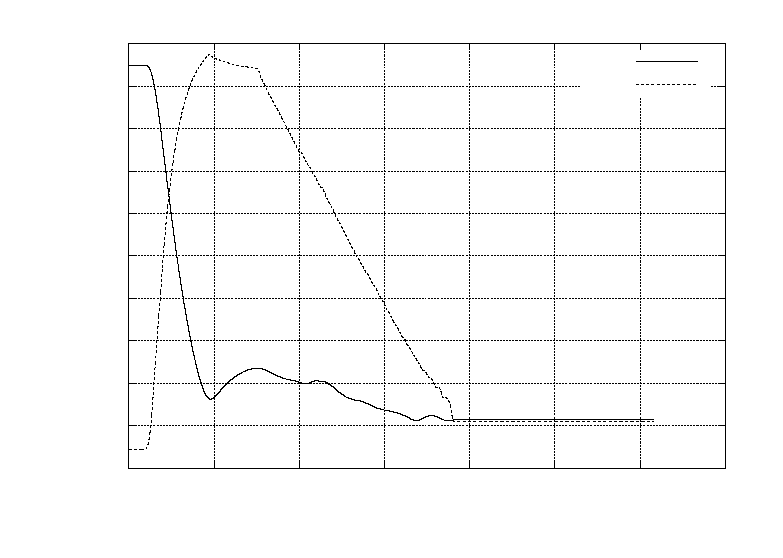
\includegraphics[width=0.49\textwidth]{static_smach_good_plot}}
        %\subfigure[Dynamic target interception.\label{f:fuz_dyn}]{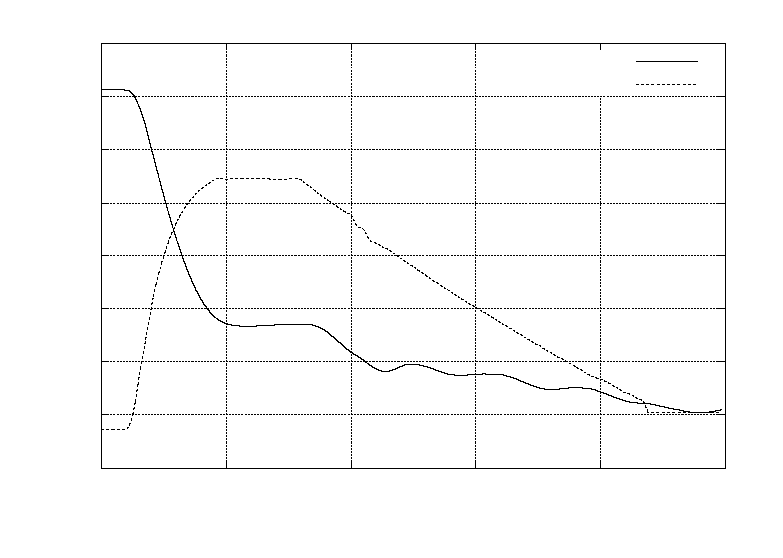
\includegraphics[width=0.49\textwidth]{moving_line_good_plot}}
    %\end{subfigmatrix}
    %\caption{Fuzzy controllers for static and dynamic landing}\label{f:fuzzy_lands}
%\end{figure}


\section{Conclusion}
It has been shown that a pure FLS controller is capable of controlling the position of a multirotor vehicle in
the task of precision landing on a small target. The small size of the platform presents a challenging
landing target; the FLS proved capable enough to overcome this challenge easily. The kalman filtering was an
integral component in providing the controller with a steady estimate of its error state. The components
chosen to accomplish this task are readily available in university laboratory environments and the physical
realization of this system was kept in the forefront of the design process. 



\chapter{Conclusions}

\section{Summary}
Genetic Fuzzy Systems are not a silver bullet solution to every problem; however, this can be said of any
architecture, paradigm, or approach. It becomes the job of an engineer to know the breadth of tools at their
disposal and be able to chose the best for a job. It is the proposition of this thesis that FL systems should
be considered as first-class citizens in the tool chest of any controls engineer. They are more than capable
of performing the low-level control tasks required in dynamics problems and are remarkably well-suited to make
decisions at higher levels as well. The ability of FLS to translate the intuition of expert controls designers
into machine-executable signals is a unique benefit that is worth exploring for a wide array of problems we
face every day.

It was shown in this work that the combination of manual construction and genetic tuning of a FLS produces a
controller which performs near-optimally in a highly non-linear system. It was also shown that a
FLS which is learned almost solely via a GA can attain results which meet any number of physically realizable
specifications. The expert intuition in these cases emerges in the development of a fitness (or cost) function
which accurately describes the desired behavior. Finally, it was shown that a purely hand-tuned system can
perform remarkably well. This system is perhaps far from optimal, but has the distinction of being
implementable on affordable hardware in real time. 

In conclusion, fuzzy logic systems and genetic fuzzy systems are valuable tools in the controls engineering
field and should be considered as viable alternatives when working with many systems. Indeed, there are many
applications in which FL control provides a nearly optimal controller and does so with minimal computational
overhead and little control effort. 

\section{Future Work}
This thesis opens the door to many opportunities for future work. First, there is still much work which could
be done with regards to the components of the controller itself. There are many corollaries to the controller
which remain unexplored. The computer vision algorithm is simplified and could be expanded greatly to produce
a much more robust and versatile application. Also, the EKF is minimally tuned, more work could be done to
produce a cleaner estimate signal.

Second, this thesis showed the effectiveness of landing a FL-controlled multirotor aircraft on a moving
platform. It is the author's belief that layering a GA-automated tuning process to the simulation would result
in even better performance. Some preliminary work has been done in developing a cost function which will aid
the development of evolutionary approaches in the future.

Third, it is the author's hope that the work will be continued in the laboratory and eventually be applied to
hardware.  The use of ROS to implement the control architecture allows this control architecture to operate in
physical hardware, as has been shown in other projects in the laboratory environment in recent projects.

Finally, integration of this work with other projects within the UAV Master Labs at the University of
Cincinnati would facilitate this project in being used in real applications. The controller could rather
easily be ported into the $\mathbbm{FlyMASTER}$ framework as a controller module. This would ease the
integration of this work with other projects in the future and work towards the goal of unifying many projects
in the lab towards a greater whole.






\bibliographystyle{unsrt}
\bibliography{fuzzy}

\appendix
\chapter{Static landing sequence state machine video description}\label{app:smach}
The following screen shots come from a video of a simulation using the kalman filter and fuzzy controller,
landing the vehicle on a stationary platform (\crefrange{f:smach_arm}{f:smach_complete}). The
video shows the simulation environment on the left of the screen, and tracks progress of the
state machine on the right of the screen.  Any active state in the state diagram is highlighted in green.
Multiple states are commonly active at the same time. As a state is completed, its color reverts. In the
screenshots, you can clearly see the vehicle taking off, traveling to the communicated waypoint, locating and
locking the location of the platform via image recognition, and initiating the approach and land states.

\begin{figure}
    \centering
    \includegraphics[width=0.8\textwidth]{images/static_captures/static-15h38m02s451}
    \caption{The ``ARM'' state as the vehicle is arming its motors.}\label{f:smach_arm}
\end{figure}


\begin{figure}
    \centering
    \includegraphics[width=0.8\textwidth]{images/static_captures/static-17h12m13s811}
    \caption{The transition to ``TRACK'' sends the command to go to a waypoint via the ``SEEK'' substate. The
        vehicle immediately takes off and navigates to the commanded position. During this state, the
        covariance is monitored to trigger the transition to the next state
    (``COV\_MONITOR'').}\label{f:smach_track}
\end{figure}

\begin{figure}
    \centering
    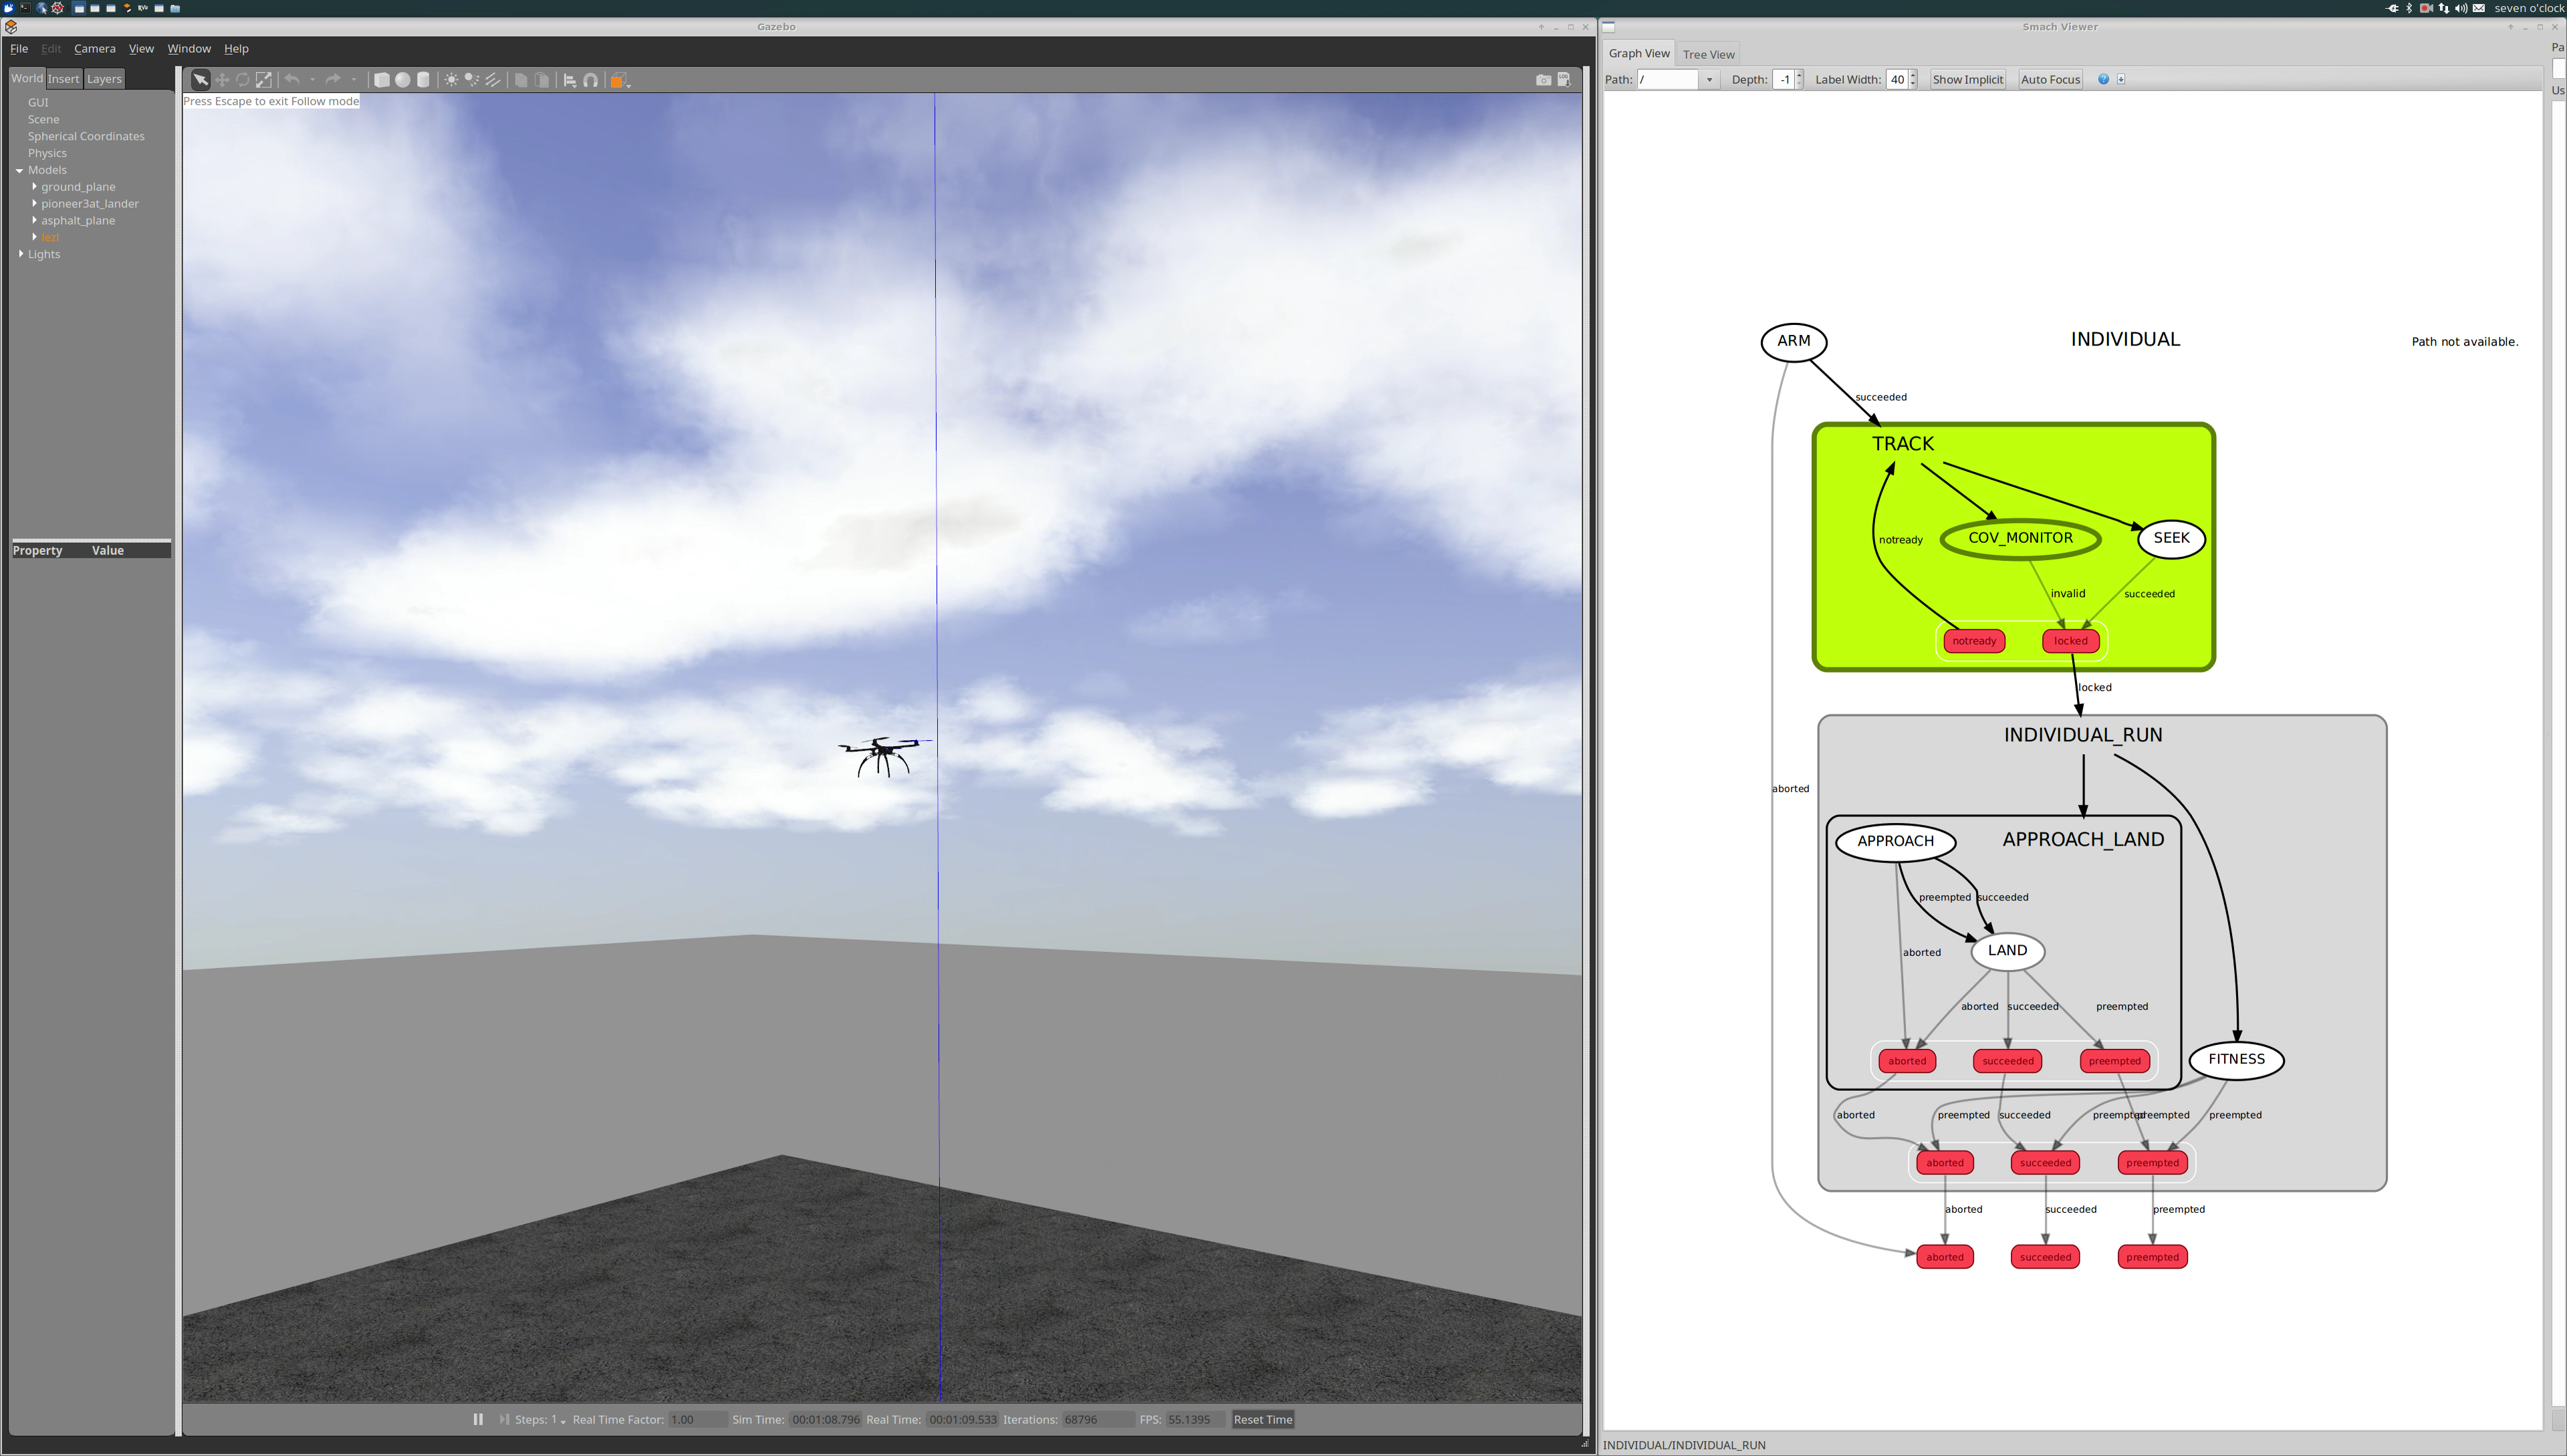
\includegraphics[width=0.8\textwidth]{images/static_captures/static-15h39m11s782}
    \caption{The ``SEEK'' substate has completed and the state machine is waiting for ``COV\_MONITOR'' to
        verify that the EKF estimate covariance is sufficiently small to signal that the vehicle has a visual
    track.}\label{f:smach_covmon}
\end{figure}

\begin{figure}
    \centering
    \includegraphics[width=0.8\textwidth]{images/static_captures/static-15h39m54s115}
    \caption{The vehicle has transitioned now to the landing approach. At this point, the FL controller is in
    command of the vehicle and all pose estimation is based on visual sensor feedback. The ``APPROACH'' state
will continue to apply FL control until either the vehicle is sufficiently close to the platform to transition
to the ``LAND'' state or loses track of the platform which will force the vehicle to abort it's
approach}\label{f:smach_approach}
\end{figure}

\begin{figure}
    \centering
    \includegraphics[width=0.8\textwidth]{images/static_captures/static-15h39m35s318}
    \caption{The vehicle has successfully approached the platform and started the landing
    sequence.}\label{f:smach_land}
\end{figure}

\begin{figure}
    \centering
    \includegraphics[width=0.8\textwidth]{images/static_captures/static-15h40m36s328}
    \caption{The vehicle is landed on the platform and motors are disarmed at mission
    success.}\label{f:smach_complete}
\end{figure}


\chapter{Moving target platform landing simulation video description}\label{app:moving}
In this video, the simulation appears on the left of the screen. The upper right window shows a coordinate
frame representation of the environment. It is in this that various frame transformations are. A
frame transformation is represented by a small unit coordinate system showing orientation, and a line to some
parent frame denoting translation. There will be four frames representing the vehicle. These four frames are
the three estimates (visual, AprilTag, EKF) and simulation truth. The images show that before the on-board
camera can see the platform, the EKF estimate is invalid as it has no data. Once the platform appears in the
image, an EKF estimate starts to converge. When the vehicle is close enough to the platform to resolve the
AprilTag, the estimate accuracy increases and continues to converge on truth until the vehicle has landed.

Also shown in the images are the raw camera feed (below and to the left of the coordinate frames) and the
AprilTag detection images (to the right of the raw feed).

\begin{figure}
    \centering
    \includegraphics[width=0.90\textwidth]{images/moving_capture/moving-18h10m27s752}
    \caption{The vehicle before its camera has had an opportunity to image the target. Truth data is the only
    frame depicted in the coordinate transformation space.}\label{f:tf_truth}
\end{figure}

\begin{figure}
    \centering
    \includegraphics[width=0.90\textwidth]{images/moving_capture/moving-18h10m47s367}
    \caption{The state of the simulation shortly after the platform has come into view. Note that the platform
    is shown in the camera's image feed, but there is no AprilTag detection as the vehicle is too far away to
resolve the tag. The EKF coordinate frame is now visible, but not yet stable. Note that the visual estimate
frame is a child of the platform frame.}\label{f:tf_visual}
\end{figure}

\begin{figure}
    \centering
    \includegraphics[width=0.90\textwidth]{images/moving_capture/moving-18h11m05s017}
    \caption{After some small amount of time, the EKF estimate has now started to converge onto truth data,
        but still shows large error as the visual estimate from the camera is the only input as of
    yet.}\label{f:tf_visual2}
\end{figure}

\begin{figure}
    \centering
    \includegraphics[width=0.90\textwidth]{images/moving_capture/moving-18h44m18s729}
    \caption{The AprilTag has now returned a detection and the EKF estimate is likewise converging towards
    truth with two estimate to fuse together.}\label{f:tf_april}
\end{figure}

\begin{figure}
    \centering
    \includegraphics[width=0.90\textwidth]{images/moving_capture/moving-18h12m15s888}
    \caption{The simulation state just before the landing sequence has completed. The estimates at this range
    are very reliable.}\label{f:tf_final}
\end{figure}




\end{document}




